\chapter{Automatic composition}
\minitoc
\mynote{Debug minitoc}

% **************************** Define Graphics Path **************************
\ifpdf
    \graphicspath{{Chapter4/Figs/Raster/}{Chapter4/Figs/PDF/}{Chapter4/Figs/}}
\else
    \graphicspath{{Chapter4/Figs/Vector/}{Chapter4/Figs/}}
\fi


This chapter describes a generative RNN sequence model for polyphonic music. We
first describe our process for constructing a training corpus of chorales and
quantify the impact of our preprocessing procedure over the corpus. Next, we
present a simple frame-based sequence encoding for polyphonic music. Using this
sequence representation, we perform an investigation of various RNN
architectures, design tradeoffs, and training methods. The results of our
investigation are used to design our final model, which we compare against
prior work and utilize in following chapters.

\section{Constructing a corpus of encoded scores}

We restrict the scope of our investigation to Bach chorales for the following reasons:
\begin{enumerate}
  \item The Baroque style employed in Bach chorales has specific guidelines
    \citep{piston1978harmony} (i.e.\ no parallel fifths) and stylistic elements
    (i.e. voice leading) which can be use to qualitatively evaluate success
  \item The structure of chorales are regular: all chorales have four parts and
    consist of a melody in the Soprano part harmonized by the Alto, Tenor, and
    Bass parts. Additionally, each chorale consists of a series of \emph{phrases}:
    groupings of consecutive notes into a unit that has complete musical sense
    of its own\citep{nattiez1990music}. It is well known\mynote{citep} that Bach
    denoted ends of phrases with fermatas\mynote{refer back to background}.
  \item The Bach chorales have become a standardized corpus routinely studied
    by aspiring music theorists\citep{white2002guidelines}
\end{enumerate}
The Bach chorales, indexed by the Bach-Werke-Verzeichnis (BWV) numbering
system\citep{butt1999bach}, are conveniently provided by
\texttt{music21}\citep{Scott2015}.

\subsection{Preprocessing}

Motivated by the transposition invariance of music and prior practice
\citep{mozer1994neural} \citep{Eck2002} \citep{franklin2004recurrent}
\citep{franklin2005jazz}, we first perform \emph{key normalization}.
The key signature of each score were firsanalyzed using the Krumhansl
Schmuckler key-finding algorithm \citep{krumhansl2001cognitive} and then
transposed according to \mynote{Table XYZ} such that the transposed key is
C-major for major mode scores and A-minor for minor mode scores.

Next, we perform \emph{time quantization} by aligning note start and end times
to the nearest multiple of some minimum duration. Our model uses a minimum
duration of one $1/16$th note, exceeding the time resoltuions of
\citep{Boulanger-Lewandowski2012} \citep{Eck2002} by 2x,
\citep{hild1991harmonet} by 4x, and \citep{bellgard1994harmonizing} by 8x.

We consider only note pitches and durations, neglecting changes in timing
(e.g. ritardandos), dynamics (e.g. crescendos), and stylistic notations (e.g.
accents, staccatos, legatos).

An example of the distortion introduced through of our preprocessing steps is
provided in \vref{fig:score-effects-preproc} in sheet music notation and in
piano roll\mynote{Is piano roll defined?} notation on
\vref{fig:piano-roll-effects-preproc}.
\begin{figure}[p]
    \centering
    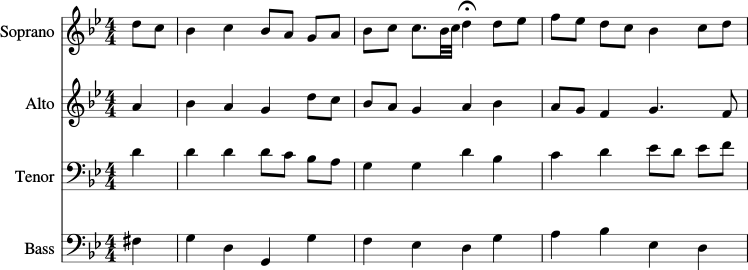
\includegraphics[width=0.8\linewidth]{bwv185-6-original-score-1.png}
    \vspace{1cm}
    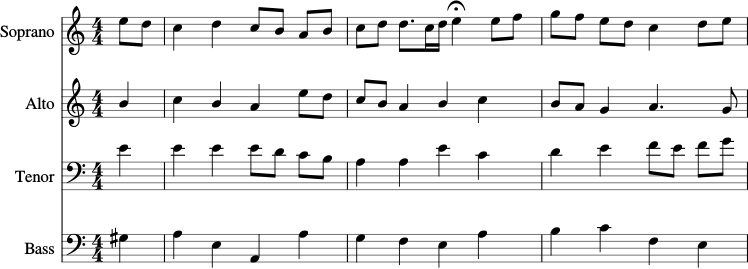
\includegraphics[width=0.8\linewidth]{bwv185-6-preproc-score-1.png}
    \caption{First 4 bars of JCB Chorale BWV 133.6 before (top) and after (bottom) preprocessing. Note
    the transposition down by a semitone to C-major as well as quantization of the
    demisemiquavers in the third bar of the Soprano part.}
    \label{fig:score-effects-preproc}
\end{figure}

\begin{figure}[tb]
    \centering
        %% Creator: Matplotlib, PGF backend
%%
%% To include the figure in your LaTeX document, write
%%   \input{<filename>.pgf}
%%
%% Make sure the required packages are loaded in your preamble
%%   \usepackage{pgf}
%%
%% Figures using additional raster images can only be included by \input if
%% they are in the same directory as the main LaTeX file. For loading figures
%% from other directories you can use the `import` package
%%   \usepackage{import}
%% and then include the figures with
%%   \import{<path to file>}{<filename>.pgf}
%%
%% Matplotlib used the following preamble
%%   \usepackage[utf8x]{inputenc}
%%   \usepackage[T1]{fontenc}
%%   \usepackage{fontspec}
%%
\begingroup%
\makeatletter%
\begin{pgfpicture}%
\pgfpathrectangle{\pgfpointorigin}{\pgfqpoint{4.900950in}{1.901007in}}%
\pgfusepath{use as bounding box, clip}%
\begin{pgfscope}%
\pgfsetbuttcap%
\pgfsetmiterjoin%
\definecolor{currentfill}{rgb}{1.000000,1.000000,1.000000}%
\pgfsetfillcolor{currentfill}%
\pgfsetlinewidth{0.000000pt}%
\definecolor{currentstroke}{rgb}{1.000000,1.000000,1.000000}%
\pgfsetstrokecolor{currentstroke}%
\pgfsetdash{}{0pt}%
\pgfpathmoveto{\pgfqpoint{0.000000in}{0.000000in}}%
\pgfpathlineto{\pgfqpoint{4.900950in}{0.000000in}}%
\pgfpathlineto{\pgfqpoint{4.900950in}{1.901007in}}%
\pgfpathlineto{\pgfqpoint{0.000000in}{1.901007in}}%
\pgfpathclose%
\pgfusepath{fill}%
\end{pgfscope}%
\begin{pgfscope}%
\pgfsetbuttcap%
\pgfsetmiterjoin%
\definecolor{currentfill}{rgb}{0.917647,0.917647,0.949020}%
\pgfsetfillcolor{currentfill}%
\pgfsetlinewidth{0.000000pt}%
\definecolor{currentstroke}{rgb}{0.000000,0.000000,0.000000}%
\pgfsetstrokecolor{currentstroke}%
\pgfsetstrokeopacity{0.000000}%
\pgfsetdash{}{0pt}%
\pgfpathmoveto{\pgfqpoint{0.554271in}{0.464000in}}%
\pgfpathlineto{\pgfqpoint{4.800950in}{0.464000in}}%
\pgfpathlineto{\pgfqpoint{4.800950in}{1.606563in}}%
\pgfpathlineto{\pgfqpoint{0.554271in}{1.606563in}}%
\pgfpathclose%
\pgfusepath{fill}%
\end{pgfscope}%
\begin{pgfscope}%
\pgfpathrectangle{\pgfqpoint{0.554271in}{0.464000in}}{\pgfqpoint{4.246679in}{1.142563in}} %
\pgfusepath{clip}%
\pgfsetroundcap%
\pgfsetroundjoin%
\pgfsetlinewidth{1.003750pt}%
\definecolor{currentstroke}{rgb}{1.000000,1.000000,1.000000}%
\pgfsetstrokecolor{currentstroke}%
\pgfsetdash{}{0pt}%
\pgfpathmoveto{\pgfqpoint{0.554271in}{0.464000in}}%
\pgfpathlineto{\pgfqpoint{0.554271in}{1.606563in}}%
\pgfusepath{stroke}%
\end{pgfscope}%
\begin{pgfscope}%
\pgfsetbuttcap%
\pgfsetroundjoin%
\definecolor{currentfill}{rgb}{0.501961,0.501961,0.501961}%
\pgfsetfillcolor{currentfill}%
\pgfsetlinewidth{1.003750pt}%
\definecolor{currentstroke}{rgb}{0.501961,0.501961,0.501961}%
\pgfsetstrokecolor{currentstroke}%
\pgfsetdash{}{0pt}%
\pgfsys@defobject{currentmarker}{\pgfqpoint{0.000000in}{0.000000in}}{\pgfqpoint{0.000000in}{0.000000in}}{%
\pgfpathmoveto{\pgfqpoint{0.000000in}{0.000000in}}%
\pgfpathlineto{\pgfqpoint{0.000000in}{0.000000in}}%
\pgfusepath{stroke,fill}%
}%
\begin{pgfscope}%
\pgfsys@transformshift{0.554271in}{0.464000in}%
\pgfsys@useobject{currentmarker}{}%
\end{pgfscope}%
\end{pgfscope}%
\begin{pgfscope}%
\definecolor{textcolor}{rgb}{0.150000,0.150000,0.150000}%
\pgfsetstrokecolor{textcolor}%
\pgfsetfillcolor{textcolor}%
\pgftext[x=0.554271in,y=0.366778in,,top]{\color{textcolor}\rmfamily\fontsize{6.000000}{7.200000}\selectfont 0}%
\end{pgfscope}%
\begin{pgfscope}%
\pgfpathrectangle{\pgfqpoint{0.554271in}{0.464000in}}{\pgfqpoint{4.246679in}{1.142563in}} %
\pgfusepath{clip}%
\pgfsetroundcap%
\pgfsetroundjoin%
\pgfsetlinewidth{1.003750pt}%
\definecolor{currentstroke}{rgb}{1.000000,1.000000,1.000000}%
\pgfsetstrokecolor{currentstroke}%
\pgfsetdash{}{0pt}%
\pgfpathmoveto{\pgfqpoint{0.880939in}{0.464000in}}%
\pgfpathlineto{\pgfqpoint{0.880939in}{1.606563in}}%
\pgfusepath{stroke}%
\end{pgfscope}%
\begin{pgfscope}%
\pgfsetbuttcap%
\pgfsetroundjoin%
\definecolor{currentfill}{rgb}{0.501961,0.501961,0.501961}%
\pgfsetfillcolor{currentfill}%
\pgfsetlinewidth{1.003750pt}%
\definecolor{currentstroke}{rgb}{0.501961,0.501961,0.501961}%
\pgfsetstrokecolor{currentstroke}%
\pgfsetdash{}{0pt}%
\pgfsys@defobject{currentmarker}{\pgfqpoint{0.000000in}{0.000000in}}{\pgfqpoint{0.000000in}{0.000000in}}{%
\pgfpathmoveto{\pgfqpoint{0.000000in}{0.000000in}}%
\pgfpathlineto{\pgfqpoint{0.000000in}{0.000000in}}%
\pgfusepath{stroke,fill}%
}%
\begin{pgfscope}%
\pgfsys@transformshift{0.880939in}{0.464000in}%
\pgfsys@useobject{currentmarker}{}%
\end{pgfscope}%
\end{pgfscope}%
\begin{pgfscope}%
\definecolor{textcolor}{rgb}{0.150000,0.150000,0.150000}%
\pgfsetstrokecolor{textcolor}%
\pgfsetfillcolor{textcolor}%
\pgftext[x=0.880939in,y=0.366778in,,top]{\color{textcolor}\rmfamily\fontsize{6.000000}{7.200000}\selectfont 1}%
\end{pgfscope}%
\begin{pgfscope}%
\pgfpathrectangle{\pgfqpoint{0.554271in}{0.464000in}}{\pgfqpoint{4.246679in}{1.142563in}} %
\pgfusepath{clip}%
\pgfsetroundcap%
\pgfsetroundjoin%
\pgfsetlinewidth{1.003750pt}%
\definecolor{currentstroke}{rgb}{1.000000,1.000000,1.000000}%
\pgfsetstrokecolor{currentstroke}%
\pgfsetdash{}{0pt}%
\pgfpathmoveto{\pgfqpoint{2.187609in}{0.464000in}}%
\pgfpathlineto{\pgfqpoint{2.187609in}{1.606563in}}%
\pgfusepath{stroke}%
\end{pgfscope}%
\begin{pgfscope}%
\pgfsetbuttcap%
\pgfsetroundjoin%
\definecolor{currentfill}{rgb}{0.501961,0.501961,0.501961}%
\pgfsetfillcolor{currentfill}%
\pgfsetlinewidth{1.003750pt}%
\definecolor{currentstroke}{rgb}{0.501961,0.501961,0.501961}%
\pgfsetstrokecolor{currentstroke}%
\pgfsetdash{}{0pt}%
\pgfsys@defobject{currentmarker}{\pgfqpoint{0.000000in}{0.000000in}}{\pgfqpoint{0.000000in}{0.000000in}}{%
\pgfpathmoveto{\pgfqpoint{0.000000in}{0.000000in}}%
\pgfpathlineto{\pgfqpoint{0.000000in}{0.000000in}}%
\pgfusepath{stroke,fill}%
}%
\begin{pgfscope}%
\pgfsys@transformshift{2.187609in}{0.464000in}%
\pgfsys@useobject{currentmarker}{}%
\end{pgfscope}%
\end{pgfscope}%
\begin{pgfscope}%
\definecolor{textcolor}{rgb}{0.150000,0.150000,0.150000}%
\pgfsetstrokecolor{textcolor}%
\pgfsetfillcolor{textcolor}%
\pgftext[x=2.187609in,y=0.366778in,,top]{\color{textcolor}\rmfamily\fontsize{6.000000}{7.200000}\selectfont 2}%
\end{pgfscope}%
\begin{pgfscope}%
\pgfpathrectangle{\pgfqpoint{0.554271in}{0.464000in}}{\pgfqpoint{4.246679in}{1.142563in}} %
\pgfusepath{clip}%
\pgfsetroundcap%
\pgfsetroundjoin%
\pgfsetlinewidth{1.003750pt}%
\definecolor{currentstroke}{rgb}{1.000000,1.000000,1.000000}%
\pgfsetstrokecolor{currentstroke}%
\pgfsetdash{}{0pt}%
\pgfpathmoveto{\pgfqpoint{3.494280in}{0.464000in}}%
\pgfpathlineto{\pgfqpoint{3.494280in}{1.606563in}}%
\pgfusepath{stroke}%
\end{pgfscope}%
\begin{pgfscope}%
\pgfsetbuttcap%
\pgfsetroundjoin%
\definecolor{currentfill}{rgb}{0.501961,0.501961,0.501961}%
\pgfsetfillcolor{currentfill}%
\pgfsetlinewidth{1.003750pt}%
\definecolor{currentstroke}{rgb}{0.501961,0.501961,0.501961}%
\pgfsetstrokecolor{currentstroke}%
\pgfsetdash{}{0pt}%
\pgfsys@defobject{currentmarker}{\pgfqpoint{0.000000in}{0.000000in}}{\pgfqpoint{0.000000in}{0.000000in}}{%
\pgfpathmoveto{\pgfqpoint{0.000000in}{0.000000in}}%
\pgfpathlineto{\pgfqpoint{0.000000in}{0.000000in}}%
\pgfusepath{stroke,fill}%
}%
\begin{pgfscope}%
\pgfsys@transformshift{3.494280in}{0.464000in}%
\pgfsys@useobject{currentmarker}{}%
\end{pgfscope}%
\end{pgfscope}%
\begin{pgfscope}%
\definecolor{textcolor}{rgb}{0.150000,0.150000,0.150000}%
\pgfsetstrokecolor{textcolor}%
\pgfsetfillcolor{textcolor}%
\pgftext[x=3.494280in,y=0.366778in,,top]{\color{textcolor}\rmfamily\fontsize{6.000000}{7.200000}\selectfont 3}%
\end{pgfscope}%
\begin{pgfscope}%
\definecolor{textcolor}{rgb}{0.150000,0.150000,0.150000}%
\pgfsetstrokecolor{textcolor}%
\pgfsetfillcolor{textcolor}%
\pgftext[x=2.677611in,y=0.223333in,,top]{\color{textcolor}\rmfamily\fontsize{10.000000}{12.000000}\selectfont Measure number}%
\end{pgfscope}%
\begin{pgfscope}%
\pgfpathrectangle{\pgfqpoint{0.554271in}{0.464000in}}{\pgfqpoint{4.246679in}{1.142563in}} %
\pgfusepath{clip}%
\pgfsetroundcap%
\pgfsetroundjoin%
\pgfsetlinewidth{1.003750pt}%
\definecolor{currentstroke}{rgb}{1.000000,1.000000,1.000000}%
\pgfsetstrokecolor{currentstroke}%
\pgfsetdash{}{0pt}%
\pgfpathmoveto{\pgfqpoint{0.554271in}{0.512277in}}%
\pgfpathlineto{\pgfqpoint{4.800950in}{0.512277in}}%
\pgfusepath{stroke}%
\end{pgfscope}%
\begin{pgfscope}%
\pgfsetbuttcap%
\pgfsetroundjoin%
\definecolor{currentfill}{rgb}{0.501961,0.501961,0.501961}%
\pgfsetfillcolor{currentfill}%
\pgfsetlinewidth{1.003750pt}%
\definecolor{currentstroke}{rgb}{0.501961,0.501961,0.501961}%
\pgfsetstrokecolor{currentstroke}%
\pgfsetdash{}{0pt}%
\pgfsys@defobject{currentmarker}{\pgfqpoint{0.000000in}{0.000000in}}{\pgfqpoint{0.000000in}{0.000000in}}{%
\pgfpathmoveto{\pgfqpoint{0.000000in}{0.000000in}}%
\pgfpathlineto{\pgfqpoint{0.000000in}{0.000000in}}%
\pgfusepath{stroke,fill}%
}%
\begin{pgfscope}%
\pgfsys@transformshift{0.554271in}{0.512277in}%
\pgfsys@useobject{currentmarker}{}%
\end{pgfscope}%
\end{pgfscope}%
\begin{pgfscope}%
\definecolor{textcolor}{rgb}{0.150000,0.150000,0.150000}%
\pgfsetstrokecolor{textcolor}%
\pgfsetfillcolor{textcolor}%
\pgftext[x=0.457049in,y=0.512277in,right,]{\color{textcolor}\rmfamily\fontsize{6.000000}{7.200000}\selectfont G2}%
\end{pgfscope}%
\begin{pgfscope}%
\pgfpathrectangle{\pgfqpoint{0.554271in}{0.464000in}}{\pgfqpoint{4.246679in}{1.142563in}} %
\pgfusepath{clip}%
\pgfsetroundcap%
\pgfsetroundjoin%
\pgfsetlinewidth{1.003750pt}%
\definecolor{currentstroke}{rgb}{1.000000,1.000000,1.000000}%
\pgfsetstrokecolor{currentstroke}%
\pgfsetdash{}{0pt}%
\pgfpathmoveto{\pgfqpoint{0.554271in}{0.544462in}}%
\pgfpathlineto{\pgfqpoint{4.800950in}{0.544462in}}%
\pgfusepath{stroke}%
\end{pgfscope}%
\begin{pgfscope}%
\pgfsetbuttcap%
\pgfsetroundjoin%
\definecolor{currentfill}{rgb}{0.501961,0.501961,0.501961}%
\pgfsetfillcolor{currentfill}%
\pgfsetlinewidth{1.003750pt}%
\definecolor{currentstroke}{rgb}{0.501961,0.501961,0.501961}%
\pgfsetstrokecolor{currentstroke}%
\pgfsetdash{}{0pt}%
\pgfsys@defobject{currentmarker}{\pgfqpoint{0.000000in}{0.000000in}}{\pgfqpoint{0.000000in}{0.000000in}}{%
\pgfpathmoveto{\pgfqpoint{0.000000in}{0.000000in}}%
\pgfpathlineto{\pgfqpoint{0.000000in}{0.000000in}}%
\pgfusepath{stroke,fill}%
}%
\begin{pgfscope}%
\pgfsys@transformshift{0.554271in}{0.544462in}%
\pgfsys@useobject{currentmarker}{}%
\end{pgfscope}%
\end{pgfscope}%
\begin{pgfscope}%
\pgfpathrectangle{\pgfqpoint{0.554271in}{0.464000in}}{\pgfqpoint{4.246679in}{1.142563in}} %
\pgfusepath{clip}%
\pgfsetroundcap%
\pgfsetroundjoin%
\pgfsetlinewidth{1.003750pt}%
\definecolor{currentstroke}{rgb}{1.000000,1.000000,1.000000}%
\pgfsetstrokecolor{currentstroke}%
\pgfsetdash{}{0pt}%
\pgfpathmoveto{\pgfqpoint{0.554271in}{0.576647in}}%
\pgfpathlineto{\pgfqpoint{4.800950in}{0.576647in}}%
\pgfusepath{stroke}%
\end{pgfscope}%
\begin{pgfscope}%
\pgfsetbuttcap%
\pgfsetroundjoin%
\definecolor{currentfill}{rgb}{0.501961,0.501961,0.501961}%
\pgfsetfillcolor{currentfill}%
\pgfsetlinewidth{1.003750pt}%
\definecolor{currentstroke}{rgb}{0.501961,0.501961,0.501961}%
\pgfsetstrokecolor{currentstroke}%
\pgfsetdash{}{0pt}%
\pgfsys@defobject{currentmarker}{\pgfqpoint{0.000000in}{0.000000in}}{\pgfqpoint{0.000000in}{0.000000in}}{%
\pgfpathmoveto{\pgfqpoint{0.000000in}{0.000000in}}%
\pgfpathlineto{\pgfqpoint{0.000000in}{0.000000in}}%
\pgfusepath{stroke,fill}%
}%
\begin{pgfscope}%
\pgfsys@transformshift{0.554271in}{0.576647in}%
\pgfsys@useobject{currentmarker}{}%
\end{pgfscope}%
\end{pgfscope}%
\begin{pgfscope}%
\pgfpathrectangle{\pgfqpoint{0.554271in}{0.464000in}}{\pgfqpoint{4.246679in}{1.142563in}} %
\pgfusepath{clip}%
\pgfsetroundcap%
\pgfsetroundjoin%
\pgfsetlinewidth{1.003750pt}%
\definecolor{currentstroke}{rgb}{1.000000,1.000000,1.000000}%
\pgfsetstrokecolor{currentstroke}%
\pgfsetdash{}{0pt}%
\pgfpathmoveto{\pgfqpoint{0.554271in}{0.608832in}}%
\pgfpathlineto{\pgfqpoint{4.800950in}{0.608832in}}%
\pgfusepath{stroke}%
\end{pgfscope}%
\begin{pgfscope}%
\pgfsetbuttcap%
\pgfsetroundjoin%
\definecolor{currentfill}{rgb}{0.501961,0.501961,0.501961}%
\pgfsetfillcolor{currentfill}%
\pgfsetlinewidth{1.003750pt}%
\definecolor{currentstroke}{rgb}{0.501961,0.501961,0.501961}%
\pgfsetstrokecolor{currentstroke}%
\pgfsetdash{}{0pt}%
\pgfsys@defobject{currentmarker}{\pgfqpoint{0.000000in}{0.000000in}}{\pgfqpoint{0.000000in}{0.000000in}}{%
\pgfpathmoveto{\pgfqpoint{0.000000in}{0.000000in}}%
\pgfpathlineto{\pgfqpoint{0.000000in}{0.000000in}}%
\pgfusepath{stroke,fill}%
}%
\begin{pgfscope}%
\pgfsys@transformshift{0.554271in}{0.608832in}%
\pgfsys@useobject{currentmarker}{}%
\end{pgfscope}%
\end{pgfscope}%
\begin{pgfscope}%
\pgfpathrectangle{\pgfqpoint{0.554271in}{0.464000in}}{\pgfqpoint{4.246679in}{1.142563in}} %
\pgfusepath{clip}%
\pgfsetroundcap%
\pgfsetroundjoin%
\pgfsetlinewidth{1.003750pt}%
\definecolor{currentstroke}{rgb}{1.000000,1.000000,1.000000}%
\pgfsetstrokecolor{currentstroke}%
\pgfsetdash{}{0pt}%
\pgfpathmoveto{\pgfqpoint{0.554271in}{0.641017in}}%
\pgfpathlineto{\pgfqpoint{4.800950in}{0.641017in}}%
\pgfusepath{stroke}%
\end{pgfscope}%
\begin{pgfscope}%
\pgfsetbuttcap%
\pgfsetroundjoin%
\definecolor{currentfill}{rgb}{0.501961,0.501961,0.501961}%
\pgfsetfillcolor{currentfill}%
\pgfsetlinewidth{1.003750pt}%
\definecolor{currentstroke}{rgb}{0.501961,0.501961,0.501961}%
\pgfsetstrokecolor{currentstroke}%
\pgfsetdash{}{0pt}%
\pgfsys@defobject{currentmarker}{\pgfqpoint{0.000000in}{0.000000in}}{\pgfqpoint{0.000000in}{0.000000in}}{%
\pgfpathmoveto{\pgfqpoint{0.000000in}{0.000000in}}%
\pgfpathlineto{\pgfqpoint{0.000000in}{0.000000in}}%
\pgfusepath{stroke,fill}%
}%
\begin{pgfscope}%
\pgfsys@transformshift{0.554271in}{0.641017in}%
\pgfsys@useobject{currentmarker}{}%
\end{pgfscope}%
\end{pgfscope}%
\begin{pgfscope}%
\pgfpathrectangle{\pgfqpoint{0.554271in}{0.464000in}}{\pgfqpoint{4.246679in}{1.142563in}} %
\pgfusepath{clip}%
\pgfsetroundcap%
\pgfsetroundjoin%
\pgfsetlinewidth{1.003750pt}%
\definecolor{currentstroke}{rgb}{1.000000,1.000000,1.000000}%
\pgfsetstrokecolor{currentstroke}%
\pgfsetdash{}{0pt}%
\pgfpathmoveto{\pgfqpoint{0.554271in}{0.673201in}}%
\pgfpathlineto{\pgfqpoint{4.800950in}{0.673201in}}%
\pgfusepath{stroke}%
\end{pgfscope}%
\begin{pgfscope}%
\pgfsetbuttcap%
\pgfsetroundjoin%
\definecolor{currentfill}{rgb}{0.501961,0.501961,0.501961}%
\pgfsetfillcolor{currentfill}%
\pgfsetlinewidth{1.003750pt}%
\definecolor{currentstroke}{rgb}{0.501961,0.501961,0.501961}%
\pgfsetstrokecolor{currentstroke}%
\pgfsetdash{}{0pt}%
\pgfsys@defobject{currentmarker}{\pgfqpoint{0.000000in}{0.000000in}}{\pgfqpoint{0.000000in}{0.000000in}}{%
\pgfpathmoveto{\pgfqpoint{0.000000in}{0.000000in}}%
\pgfpathlineto{\pgfqpoint{0.000000in}{0.000000in}}%
\pgfusepath{stroke,fill}%
}%
\begin{pgfscope}%
\pgfsys@transformshift{0.554271in}{0.673201in}%
\pgfsys@useobject{currentmarker}{}%
\end{pgfscope}%
\end{pgfscope}%
\begin{pgfscope}%
\pgfpathrectangle{\pgfqpoint{0.554271in}{0.464000in}}{\pgfqpoint{4.246679in}{1.142563in}} %
\pgfusepath{clip}%
\pgfsetroundcap%
\pgfsetroundjoin%
\pgfsetlinewidth{1.003750pt}%
\definecolor{currentstroke}{rgb}{1.000000,1.000000,1.000000}%
\pgfsetstrokecolor{currentstroke}%
\pgfsetdash{}{0pt}%
\pgfpathmoveto{\pgfqpoint{0.554271in}{0.705386in}}%
\pgfpathlineto{\pgfqpoint{4.800950in}{0.705386in}}%
\pgfusepath{stroke}%
\end{pgfscope}%
\begin{pgfscope}%
\pgfsetbuttcap%
\pgfsetroundjoin%
\definecolor{currentfill}{rgb}{0.501961,0.501961,0.501961}%
\pgfsetfillcolor{currentfill}%
\pgfsetlinewidth{1.003750pt}%
\definecolor{currentstroke}{rgb}{0.501961,0.501961,0.501961}%
\pgfsetstrokecolor{currentstroke}%
\pgfsetdash{}{0pt}%
\pgfsys@defobject{currentmarker}{\pgfqpoint{0.000000in}{0.000000in}}{\pgfqpoint{0.000000in}{0.000000in}}{%
\pgfpathmoveto{\pgfqpoint{0.000000in}{0.000000in}}%
\pgfpathlineto{\pgfqpoint{0.000000in}{0.000000in}}%
\pgfusepath{stroke,fill}%
}%
\begin{pgfscope}%
\pgfsys@transformshift{0.554271in}{0.705386in}%
\pgfsys@useobject{currentmarker}{}%
\end{pgfscope}%
\end{pgfscope}%
\begin{pgfscope}%
\pgfpathrectangle{\pgfqpoint{0.554271in}{0.464000in}}{\pgfqpoint{4.246679in}{1.142563in}} %
\pgfusepath{clip}%
\pgfsetroundcap%
\pgfsetroundjoin%
\pgfsetlinewidth{1.003750pt}%
\definecolor{currentstroke}{rgb}{1.000000,1.000000,1.000000}%
\pgfsetstrokecolor{currentstroke}%
\pgfsetdash{}{0pt}%
\pgfpathmoveto{\pgfqpoint{0.554271in}{0.737571in}}%
\pgfpathlineto{\pgfqpoint{4.800950in}{0.737571in}}%
\pgfusepath{stroke}%
\end{pgfscope}%
\begin{pgfscope}%
\pgfsetbuttcap%
\pgfsetroundjoin%
\definecolor{currentfill}{rgb}{0.501961,0.501961,0.501961}%
\pgfsetfillcolor{currentfill}%
\pgfsetlinewidth{1.003750pt}%
\definecolor{currentstroke}{rgb}{0.501961,0.501961,0.501961}%
\pgfsetstrokecolor{currentstroke}%
\pgfsetdash{}{0pt}%
\pgfsys@defobject{currentmarker}{\pgfqpoint{0.000000in}{0.000000in}}{\pgfqpoint{0.000000in}{0.000000in}}{%
\pgfpathmoveto{\pgfqpoint{0.000000in}{0.000000in}}%
\pgfpathlineto{\pgfqpoint{0.000000in}{0.000000in}}%
\pgfusepath{stroke,fill}%
}%
\begin{pgfscope}%
\pgfsys@transformshift{0.554271in}{0.737571in}%
\pgfsys@useobject{currentmarker}{}%
\end{pgfscope}%
\end{pgfscope}%
\begin{pgfscope}%
\definecolor{textcolor}{rgb}{0.150000,0.150000,0.150000}%
\pgfsetstrokecolor{textcolor}%
\pgfsetfillcolor{textcolor}%
\pgftext[x=0.457049in,y=0.737571in,right,]{\color{textcolor}\rmfamily\fontsize{6.000000}{7.200000}\selectfont D3}%
\end{pgfscope}%
\begin{pgfscope}%
\pgfpathrectangle{\pgfqpoint{0.554271in}{0.464000in}}{\pgfqpoint{4.246679in}{1.142563in}} %
\pgfusepath{clip}%
\pgfsetroundcap%
\pgfsetroundjoin%
\pgfsetlinewidth{1.003750pt}%
\definecolor{currentstroke}{rgb}{1.000000,1.000000,1.000000}%
\pgfsetstrokecolor{currentstroke}%
\pgfsetdash{}{0pt}%
\pgfpathmoveto{\pgfqpoint{0.554271in}{0.769756in}}%
\pgfpathlineto{\pgfqpoint{4.800950in}{0.769756in}}%
\pgfusepath{stroke}%
\end{pgfscope}%
\begin{pgfscope}%
\pgfsetbuttcap%
\pgfsetroundjoin%
\definecolor{currentfill}{rgb}{0.501961,0.501961,0.501961}%
\pgfsetfillcolor{currentfill}%
\pgfsetlinewidth{1.003750pt}%
\definecolor{currentstroke}{rgb}{0.501961,0.501961,0.501961}%
\pgfsetstrokecolor{currentstroke}%
\pgfsetdash{}{0pt}%
\pgfsys@defobject{currentmarker}{\pgfqpoint{0.000000in}{0.000000in}}{\pgfqpoint{0.000000in}{0.000000in}}{%
\pgfpathmoveto{\pgfqpoint{0.000000in}{0.000000in}}%
\pgfpathlineto{\pgfqpoint{0.000000in}{0.000000in}}%
\pgfusepath{stroke,fill}%
}%
\begin{pgfscope}%
\pgfsys@transformshift{0.554271in}{0.769756in}%
\pgfsys@useobject{currentmarker}{}%
\end{pgfscope}%
\end{pgfscope}%
\begin{pgfscope}%
\definecolor{textcolor}{rgb}{0.150000,0.150000,0.150000}%
\pgfsetstrokecolor{textcolor}%
\pgfsetfillcolor{textcolor}%
\pgftext[x=0.457049in,y=0.769756in,right,]{\color{textcolor}\rmfamily\fontsize{6.000000}{7.200000}\selectfont E\(\displaystyle \flat\)3}%
\end{pgfscope}%
\begin{pgfscope}%
\pgfpathrectangle{\pgfqpoint{0.554271in}{0.464000in}}{\pgfqpoint{4.246679in}{1.142563in}} %
\pgfusepath{clip}%
\pgfsetroundcap%
\pgfsetroundjoin%
\pgfsetlinewidth{1.003750pt}%
\definecolor{currentstroke}{rgb}{1.000000,1.000000,1.000000}%
\pgfsetstrokecolor{currentstroke}%
\pgfsetdash{}{0pt}%
\pgfpathmoveto{\pgfqpoint{0.554271in}{0.801941in}}%
\pgfpathlineto{\pgfqpoint{4.800950in}{0.801941in}}%
\pgfusepath{stroke}%
\end{pgfscope}%
\begin{pgfscope}%
\pgfsetbuttcap%
\pgfsetroundjoin%
\definecolor{currentfill}{rgb}{0.501961,0.501961,0.501961}%
\pgfsetfillcolor{currentfill}%
\pgfsetlinewidth{1.003750pt}%
\definecolor{currentstroke}{rgb}{0.501961,0.501961,0.501961}%
\pgfsetstrokecolor{currentstroke}%
\pgfsetdash{}{0pt}%
\pgfsys@defobject{currentmarker}{\pgfqpoint{0.000000in}{0.000000in}}{\pgfqpoint{0.000000in}{0.000000in}}{%
\pgfpathmoveto{\pgfqpoint{0.000000in}{0.000000in}}%
\pgfpathlineto{\pgfqpoint{0.000000in}{0.000000in}}%
\pgfusepath{stroke,fill}%
}%
\begin{pgfscope}%
\pgfsys@transformshift{0.554271in}{0.801941in}%
\pgfsys@useobject{currentmarker}{}%
\end{pgfscope}%
\end{pgfscope}%
\begin{pgfscope}%
\pgfpathrectangle{\pgfqpoint{0.554271in}{0.464000in}}{\pgfqpoint{4.246679in}{1.142563in}} %
\pgfusepath{clip}%
\pgfsetroundcap%
\pgfsetroundjoin%
\pgfsetlinewidth{1.003750pt}%
\definecolor{currentstroke}{rgb}{1.000000,1.000000,1.000000}%
\pgfsetstrokecolor{currentstroke}%
\pgfsetdash{}{0pt}%
\pgfpathmoveto{\pgfqpoint{0.554271in}{0.834126in}}%
\pgfpathlineto{\pgfqpoint{4.800950in}{0.834126in}}%
\pgfusepath{stroke}%
\end{pgfscope}%
\begin{pgfscope}%
\pgfsetbuttcap%
\pgfsetroundjoin%
\definecolor{currentfill}{rgb}{0.501961,0.501961,0.501961}%
\pgfsetfillcolor{currentfill}%
\pgfsetlinewidth{1.003750pt}%
\definecolor{currentstroke}{rgb}{0.501961,0.501961,0.501961}%
\pgfsetstrokecolor{currentstroke}%
\pgfsetdash{}{0pt}%
\pgfsys@defobject{currentmarker}{\pgfqpoint{0.000000in}{0.000000in}}{\pgfqpoint{0.000000in}{0.000000in}}{%
\pgfpathmoveto{\pgfqpoint{0.000000in}{0.000000in}}%
\pgfpathlineto{\pgfqpoint{0.000000in}{0.000000in}}%
\pgfusepath{stroke,fill}%
}%
\begin{pgfscope}%
\pgfsys@transformshift{0.554271in}{0.834126in}%
\pgfsys@useobject{currentmarker}{}%
\end{pgfscope}%
\end{pgfscope}%
\begin{pgfscope}%
\definecolor{textcolor}{rgb}{0.150000,0.150000,0.150000}%
\pgfsetstrokecolor{textcolor}%
\pgfsetfillcolor{textcolor}%
\pgftext[x=0.457049in,y=0.834126in,right,]{\color{textcolor}\rmfamily\fontsize{6.000000}{7.200000}\selectfont F3}%
\end{pgfscope}%
\begin{pgfscope}%
\pgfpathrectangle{\pgfqpoint{0.554271in}{0.464000in}}{\pgfqpoint{4.246679in}{1.142563in}} %
\pgfusepath{clip}%
\pgfsetroundcap%
\pgfsetroundjoin%
\pgfsetlinewidth{1.003750pt}%
\definecolor{currentstroke}{rgb}{1.000000,1.000000,1.000000}%
\pgfsetstrokecolor{currentstroke}%
\pgfsetdash{}{0pt}%
\pgfpathmoveto{\pgfqpoint{0.554271in}{0.866311in}}%
\pgfpathlineto{\pgfqpoint{4.800950in}{0.866311in}}%
\pgfusepath{stroke}%
\end{pgfscope}%
\begin{pgfscope}%
\pgfsetbuttcap%
\pgfsetroundjoin%
\definecolor{currentfill}{rgb}{0.501961,0.501961,0.501961}%
\pgfsetfillcolor{currentfill}%
\pgfsetlinewidth{1.003750pt}%
\definecolor{currentstroke}{rgb}{0.501961,0.501961,0.501961}%
\pgfsetstrokecolor{currentstroke}%
\pgfsetdash{}{0pt}%
\pgfsys@defobject{currentmarker}{\pgfqpoint{0.000000in}{0.000000in}}{\pgfqpoint{0.000000in}{0.000000in}}{%
\pgfpathmoveto{\pgfqpoint{0.000000in}{0.000000in}}%
\pgfpathlineto{\pgfqpoint{0.000000in}{0.000000in}}%
\pgfusepath{stroke,fill}%
}%
\begin{pgfscope}%
\pgfsys@transformshift{0.554271in}{0.866311in}%
\pgfsys@useobject{currentmarker}{}%
\end{pgfscope}%
\end{pgfscope}%
\begin{pgfscope}%
\definecolor{textcolor}{rgb}{0.150000,0.150000,0.150000}%
\pgfsetstrokecolor{textcolor}%
\pgfsetfillcolor{textcolor}%
\pgftext[x=0.457049in,y=0.866311in,right,]{\color{textcolor}\rmfamily\fontsize{6.000000}{7.200000}\selectfont F\(\displaystyle \sharp\)3}%
\end{pgfscope}%
\begin{pgfscope}%
\pgfpathrectangle{\pgfqpoint{0.554271in}{0.464000in}}{\pgfqpoint{4.246679in}{1.142563in}} %
\pgfusepath{clip}%
\pgfsetroundcap%
\pgfsetroundjoin%
\pgfsetlinewidth{1.003750pt}%
\definecolor{currentstroke}{rgb}{1.000000,1.000000,1.000000}%
\pgfsetstrokecolor{currentstroke}%
\pgfsetdash{}{0pt}%
\pgfpathmoveto{\pgfqpoint{0.554271in}{0.898495in}}%
\pgfpathlineto{\pgfqpoint{4.800950in}{0.898495in}}%
\pgfusepath{stroke}%
\end{pgfscope}%
\begin{pgfscope}%
\pgfsetbuttcap%
\pgfsetroundjoin%
\definecolor{currentfill}{rgb}{0.501961,0.501961,0.501961}%
\pgfsetfillcolor{currentfill}%
\pgfsetlinewidth{1.003750pt}%
\definecolor{currentstroke}{rgb}{0.501961,0.501961,0.501961}%
\pgfsetstrokecolor{currentstroke}%
\pgfsetdash{}{0pt}%
\pgfsys@defobject{currentmarker}{\pgfqpoint{0.000000in}{0.000000in}}{\pgfqpoint{0.000000in}{0.000000in}}{%
\pgfpathmoveto{\pgfqpoint{0.000000in}{0.000000in}}%
\pgfpathlineto{\pgfqpoint{0.000000in}{0.000000in}}%
\pgfusepath{stroke,fill}%
}%
\begin{pgfscope}%
\pgfsys@transformshift{0.554271in}{0.898495in}%
\pgfsys@useobject{currentmarker}{}%
\end{pgfscope}%
\end{pgfscope}%
\begin{pgfscope}%
\definecolor{textcolor}{rgb}{0.150000,0.150000,0.150000}%
\pgfsetstrokecolor{textcolor}%
\pgfsetfillcolor{textcolor}%
\pgftext[x=0.457049in,y=0.898495in,right,]{\color{textcolor}\rmfamily\fontsize{6.000000}{7.200000}\selectfont G3}%
\end{pgfscope}%
\begin{pgfscope}%
\pgfpathrectangle{\pgfqpoint{0.554271in}{0.464000in}}{\pgfqpoint{4.246679in}{1.142563in}} %
\pgfusepath{clip}%
\pgfsetroundcap%
\pgfsetroundjoin%
\pgfsetlinewidth{1.003750pt}%
\definecolor{currentstroke}{rgb}{1.000000,1.000000,1.000000}%
\pgfsetstrokecolor{currentstroke}%
\pgfsetdash{}{0pt}%
\pgfpathmoveto{\pgfqpoint{0.554271in}{0.930680in}}%
\pgfpathlineto{\pgfqpoint{4.800950in}{0.930680in}}%
\pgfusepath{stroke}%
\end{pgfscope}%
\begin{pgfscope}%
\pgfsetbuttcap%
\pgfsetroundjoin%
\definecolor{currentfill}{rgb}{0.501961,0.501961,0.501961}%
\pgfsetfillcolor{currentfill}%
\pgfsetlinewidth{1.003750pt}%
\definecolor{currentstroke}{rgb}{0.501961,0.501961,0.501961}%
\pgfsetstrokecolor{currentstroke}%
\pgfsetdash{}{0pt}%
\pgfsys@defobject{currentmarker}{\pgfqpoint{0.000000in}{0.000000in}}{\pgfqpoint{0.000000in}{0.000000in}}{%
\pgfpathmoveto{\pgfqpoint{0.000000in}{0.000000in}}%
\pgfpathlineto{\pgfqpoint{0.000000in}{0.000000in}}%
\pgfusepath{stroke,fill}%
}%
\begin{pgfscope}%
\pgfsys@transformshift{0.554271in}{0.930680in}%
\pgfsys@useobject{currentmarker}{}%
\end{pgfscope}%
\end{pgfscope}%
\begin{pgfscope}%
\pgfpathrectangle{\pgfqpoint{0.554271in}{0.464000in}}{\pgfqpoint{4.246679in}{1.142563in}} %
\pgfusepath{clip}%
\pgfsetroundcap%
\pgfsetroundjoin%
\pgfsetlinewidth{1.003750pt}%
\definecolor{currentstroke}{rgb}{1.000000,1.000000,1.000000}%
\pgfsetstrokecolor{currentstroke}%
\pgfsetdash{}{0pt}%
\pgfpathmoveto{\pgfqpoint{0.554271in}{0.962865in}}%
\pgfpathlineto{\pgfqpoint{4.800950in}{0.962865in}}%
\pgfusepath{stroke}%
\end{pgfscope}%
\begin{pgfscope}%
\pgfsetbuttcap%
\pgfsetroundjoin%
\definecolor{currentfill}{rgb}{0.501961,0.501961,0.501961}%
\pgfsetfillcolor{currentfill}%
\pgfsetlinewidth{1.003750pt}%
\definecolor{currentstroke}{rgb}{0.501961,0.501961,0.501961}%
\pgfsetstrokecolor{currentstroke}%
\pgfsetdash{}{0pt}%
\pgfsys@defobject{currentmarker}{\pgfqpoint{0.000000in}{0.000000in}}{\pgfqpoint{0.000000in}{0.000000in}}{%
\pgfpathmoveto{\pgfqpoint{0.000000in}{0.000000in}}%
\pgfpathlineto{\pgfqpoint{0.000000in}{0.000000in}}%
\pgfusepath{stroke,fill}%
}%
\begin{pgfscope}%
\pgfsys@transformshift{0.554271in}{0.962865in}%
\pgfsys@useobject{currentmarker}{}%
\end{pgfscope}%
\end{pgfscope}%
\begin{pgfscope}%
\definecolor{textcolor}{rgb}{0.150000,0.150000,0.150000}%
\pgfsetstrokecolor{textcolor}%
\pgfsetfillcolor{textcolor}%
\pgftext[x=0.457049in,y=0.962865in,right,]{\color{textcolor}\rmfamily\fontsize{6.000000}{7.200000}\selectfont A3}%
\end{pgfscope}%
\begin{pgfscope}%
\pgfpathrectangle{\pgfqpoint{0.554271in}{0.464000in}}{\pgfqpoint{4.246679in}{1.142563in}} %
\pgfusepath{clip}%
\pgfsetroundcap%
\pgfsetroundjoin%
\pgfsetlinewidth{1.003750pt}%
\definecolor{currentstroke}{rgb}{1.000000,1.000000,1.000000}%
\pgfsetstrokecolor{currentstroke}%
\pgfsetdash{}{0pt}%
\pgfpathmoveto{\pgfqpoint{0.554271in}{0.995050in}}%
\pgfpathlineto{\pgfqpoint{4.800950in}{0.995050in}}%
\pgfusepath{stroke}%
\end{pgfscope}%
\begin{pgfscope}%
\pgfsetbuttcap%
\pgfsetroundjoin%
\definecolor{currentfill}{rgb}{0.501961,0.501961,0.501961}%
\pgfsetfillcolor{currentfill}%
\pgfsetlinewidth{1.003750pt}%
\definecolor{currentstroke}{rgb}{0.501961,0.501961,0.501961}%
\pgfsetstrokecolor{currentstroke}%
\pgfsetdash{}{0pt}%
\pgfsys@defobject{currentmarker}{\pgfqpoint{0.000000in}{0.000000in}}{\pgfqpoint{0.000000in}{0.000000in}}{%
\pgfpathmoveto{\pgfqpoint{0.000000in}{0.000000in}}%
\pgfpathlineto{\pgfqpoint{0.000000in}{0.000000in}}%
\pgfusepath{stroke,fill}%
}%
\begin{pgfscope}%
\pgfsys@transformshift{0.554271in}{0.995050in}%
\pgfsys@useobject{currentmarker}{}%
\end{pgfscope}%
\end{pgfscope}%
\begin{pgfscope}%
\definecolor{textcolor}{rgb}{0.150000,0.150000,0.150000}%
\pgfsetstrokecolor{textcolor}%
\pgfsetfillcolor{textcolor}%
\pgftext[x=0.457049in,y=0.995050in,right,]{\color{textcolor}\rmfamily\fontsize{6.000000}{7.200000}\selectfont B\(\displaystyle \flat\)3}%
\end{pgfscope}%
\begin{pgfscope}%
\pgfpathrectangle{\pgfqpoint{0.554271in}{0.464000in}}{\pgfqpoint{4.246679in}{1.142563in}} %
\pgfusepath{clip}%
\pgfsetroundcap%
\pgfsetroundjoin%
\pgfsetlinewidth{1.003750pt}%
\definecolor{currentstroke}{rgb}{1.000000,1.000000,1.000000}%
\pgfsetstrokecolor{currentstroke}%
\pgfsetdash{}{0pt}%
\pgfpathmoveto{\pgfqpoint{0.554271in}{1.027235in}}%
\pgfpathlineto{\pgfqpoint{4.800950in}{1.027235in}}%
\pgfusepath{stroke}%
\end{pgfscope}%
\begin{pgfscope}%
\pgfsetbuttcap%
\pgfsetroundjoin%
\definecolor{currentfill}{rgb}{0.501961,0.501961,0.501961}%
\pgfsetfillcolor{currentfill}%
\pgfsetlinewidth{1.003750pt}%
\definecolor{currentstroke}{rgb}{0.501961,0.501961,0.501961}%
\pgfsetstrokecolor{currentstroke}%
\pgfsetdash{}{0pt}%
\pgfsys@defobject{currentmarker}{\pgfqpoint{0.000000in}{0.000000in}}{\pgfqpoint{0.000000in}{0.000000in}}{%
\pgfpathmoveto{\pgfqpoint{0.000000in}{0.000000in}}%
\pgfpathlineto{\pgfqpoint{0.000000in}{0.000000in}}%
\pgfusepath{stroke,fill}%
}%
\begin{pgfscope}%
\pgfsys@transformshift{0.554271in}{1.027235in}%
\pgfsys@useobject{currentmarker}{}%
\end{pgfscope}%
\end{pgfscope}%
\begin{pgfscope}%
\pgfpathrectangle{\pgfqpoint{0.554271in}{0.464000in}}{\pgfqpoint{4.246679in}{1.142563in}} %
\pgfusepath{clip}%
\pgfsetroundcap%
\pgfsetroundjoin%
\pgfsetlinewidth{1.003750pt}%
\definecolor{currentstroke}{rgb}{1.000000,1.000000,1.000000}%
\pgfsetstrokecolor{currentstroke}%
\pgfsetdash{}{0pt}%
\pgfpathmoveto{\pgfqpoint{0.554271in}{1.059420in}}%
\pgfpathlineto{\pgfqpoint{4.800950in}{1.059420in}}%
\pgfusepath{stroke}%
\end{pgfscope}%
\begin{pgfscope}%
\pgfsetbuttcap%
\pgfsetroundjoin%
\definecolor{currentfill}{rgb}{0.501961,0.501961,0.501961}%
\pgfsetfillcolor{currentfill}%
\pgfsetlinewidth{1.003750pt}%
\definecolor{currentstroke}{rgb}{0.501961,0.501961,0.501961}%
\pgfsetstrokecolor{currentstroke}%
\pgfsetdash{}{0pt}%
\pgfsys@defobject{currentmarker}{\pgfqpoint{0.000000in}{0.000000in}}{\pgfqpoint{0.000000in}{0.000000in}}{%
\pgfpathmoveto{\pgfqpoint{0.000000in}{0.000000in}}%
\pgfpathlineto{\pgfqpoint{0.000000in}{0.000000in}}%
\pgfusepath{stroke,fill}%
}%
\begin{pgfscope}%
\pgfsys@transformshift{0.554271in}{1.059420in}%
\pgfsys@useobject{currentmarker}{}%
\end{pgfscope}%
\end{pgfscope}%
\begin{pgfscope}%
\definecolor{textcolor}{rgb}{0.150000,0.150000,0.150000}%
\pgfsetstrokecolor{textcolor}%
\pgfsetfillcolor{textcolor}%
\pgftext[x=0.457049in,y=1.059420in,right,]{\color{textcolor}\rmfamily\fontsize{6.000000}{7.200000}\selectfont C4}%
\end{pgfscope}%
\begin{pgfscope}%
\pgfpathrectangle{\pgfqpoint{0.554271in}{0.464000in}}{\pgfqpoint{4.246679in}{1.142563in}} %
\pgfusepath{clip}%
\pgfsetroundcap%
\pgfsetroundjoin%
\pgfsetlinewidth{1.003750pt}%
\definecolor{currentstroke}{rgb}{1.000000,1.000000,1.000000}%
\pgfsetstrokecolor{currentstroke}%
\pgfsetdash{}{0pt}%
\pgfpathmoveto{\pgfqpoint{0.554271in}{1.091605in}}%
\pgfpathlineto{\pgfqpoint{4.800950in}{1.091605in}}%
\pgfusepath{stroke}%
\end{pgfscope}%
\begin{pgfscope}%
\pgfsetbuttcap%
\pgfsetroundjoin%
\definecolor{currentfill}{rgb}{0.501961,0.501961,0.501961}%
\pgfsetfillcolor{currentfill}%
\pgfsetlinewidth{1.003750pt}%
\definecolor{currentstroke}{rgb}{0.501961,0.501961,0.501961}%
\pgfsetstrokecolor{currentstroke}%
\pgfsetdash{}{0pt}%
\pgfsys@defobject{currentmarker}{\pgfqpoint{0.000000in}{0.000000in}}{\pgfqpoint{0.000000in}{0.000000in}}{%
\pgfpathmoveto{\pgfqpoint{0.000000in}{0.000000in}}%
\pgfpathlineto{\pgfqpoint{0.000000in}{0.000000in}}%
\pgfusepath{stroke,fill}%
}%
\begin{pgfscope}%
\pgfsys@transformshift{0.554271in}{1.091605in}%
\pgfsys@useobject{currentmarker}{}%
\end{pgfscope}%
\end{pgfscope}%
\begin{pgfscope}%
\pgfpathrectangle{\pgfqpoint{0.554271in}{0.464000in}}{\pgfqpoint{4.246679in}{1.142563in}} %
\pgfusepath{clip}%
\pgfsetroundcap%
\pgfsetroundjoin%
\pgfsetlinewidth{1.003750pt}%
\definecolor{currentstroke}{rgb}{1.000000,1.000000,1.000000}%
\pgfsetstrokecolor{currentstroke}%
\pgfsetdash{}{0pt}%
\pgfpathmoveto{\pgfqpoint{0.554271in}{1.123790in}}%
\pgfpathlineto{\pgfqpoint{4.800950in}{1.123790in}}%
\pgfusepath{stroke}%
\end{pgfscope}%
\begin{pgfscope}%
\pgfsetbuttcap%
\pgfsetroundjoin%
\definecolor{currentfill}{rgb}{0.501961,0.501961,0.501961}%
\pgfsetfillcolor{currentfill}%
\pgfsetlinewidth{1.003750pt}%
\definecolor{currentstroke}{rgb}{0.501961,0.501961,0.501961}%
\pgfsetstrokecolor{currentstroke}%
\pgfsetdash{}{0pt}%
\pgfsys@defobject{currentmarker}{\pgfqpoint{0.000000in}{0.000000in}}{\pgfqpoint{0.000000in}{0.000000in}}{%
\pgfpathmoveto{\pgfqpoint{0.000000in}{0.000000in}}%
\pgfpathlineto{\pgfqpoint{0.000000in}{0.000000in}}%
\pgfusepath{stroke,fill}%
}%
\begin{pgfscope}%
\pgfsys@transformshift{0.554271in}{1.123790in}%
\pgfsys@useobject{currentmarker}{}%
\end{pgfscope}%
\end{pgfscope}%
\begin{pgfscope}%
\definecolor{textcolor}{rgb}{0.150000,0.150000,0.150000}%
\pgfsetstrokecolor{textcolor}%
\pgfsetfillcolor{textcolor}%
\pgftext[x=0.457049in,y=1.123790in,right,]{\color{textcolor}\rmfamily\fontsize{6.000000}{7.200000}\selectfont D4}%
\end{pgfscope}%
\begin{pgfscope}%
\pgfpathrectangle{\pgfqpoint{0.554271in}{0.464000in}}{\pgfqpoint{4.246679in}{1.142563in}} %
\pgfusepath{clip}%
\pgfsetroundcap%
\pgfsetroundjoin%
\pgfsetlinewidth{1.003750pt}%
\definecolor{currentstroke}{rgb}{1.000000,1.000000,1.000000}%
\pgfsetstrokecolor{currentstroke}%
\pgfsetdash{}{0pt}%
\pgfpathmoveto{\pgfqpoint{0.554271in}{1.155974in}}%
\pgfpathlineto{\pgfqpoint{4.800950in}{1.155974in}}%
\pgfusepath{stroke}%
\end{pgfscope}%
\begin{pgfscope}%
\pgfsetbuttcap%
\pgfsetroundjoin%
\definecolor{currentfill}{rgb}{0.501961,0.501961,0.501961}%
\pgfsetfillcolor{currentfill}%
\pgfsetlinewidth{1.003750pt}%
\definecolor{currentstroke}{rgb}{0.501961,0.501961,0.501961}%
\pgfsetstrokecolor{currentstroke}%
\pgfsetdash{}{0pt}%
\pgfsys@defobject{currentmarker}{\pgfqpoint{0.000000in}{0.000000in}}{\pgfqpoint{0.000000in}{0.000000in}}{%
\pgfpathmoveto{\pgfqpoint{0.000000in}{0.000000in}}%
\pgfpathlineto{\pgfqpoint{0.000000in}{0.000000in}}%
\pgfusepath{stroke,fill}%
}%
\begin{pgfscope}%
\pgfsys@transformshift{0.554271in}{1.155974in}%
\pgfsys@useobject{currentmarker}{}%
\end{pgfscope}%
\end{pgfscope}%
\begin{pgfscope}%
\definecolor{textcolor}{rgb}{0.150000,0.150000,0.150000}%
\pgfsetstrokecolor{textcolor}%
\pgfsetfillcolor{textcolor}%
\pgftext[x=0.457049in,y=1.155974in,right,]{\color{textcolor}\rmfamily\fontsize{6.000000}{7.200000}\selectfont E\(\displaystyle \flat\)4}%
\end{pgfscope}%
\begin{pgfscope}%
\pgfpathrectangle{\pgfqpoint{0.554271in}{0.464000in}}{\pgfqpoint{4.246679in}{1.142563in}} %
\pgfusepath{clip}%
\pgfsetroundcap%
\pgfsetroundjoin%
\pgfsetlinewidth{1.003750pt}%
\definecolor{currentstroke}{rgb}{1.000000,1.000000,1.000000}%
\pgfsetstrokecolor{currentstroke}%
\pgfsetdash{}{0pt}%
\pgfpathmoveto{\pgfqpoint{0.554271in}{1.188159in}}%
\pgfpathlineto{\pgfqpoint{4.800950in}{1.188159in}}%
\pgfusepath{stroke}%
\end{pgfscope}%
\begin{pgfscope}%
\pgfsetbuttcap%
\pgfsetroundjoin%
\definecolor{currentfill}{rgb}{0.501961,0.501961,0.501961}%
\pgfsetfillcolor{currentfill}%
\pgfsetlinewidth{1.003750pt}%
\definecolor{currentstroke}{rgb}{0.501961,0.501961,0.501961}%
\pgfsetstrokecolor{currentstroke}%
\pgfsetdash{}{0pt}%
\pgfsys@defobject{currentmarker}{\pgfqpoint{0.000000in}{0.000000in}}{\pgfqpoint{0.000000in}{0.000000in}}{%
\pgfpathmoveto{\pgfqpoint{0.000000in}{0.000000in}}%
\pgfpathlineto{\pgfqpoint{0.000000in}{0.000000in}}%
\pgfusepath{stroke,fill}%
}%
\begin{pgfscope}%
\pgfsys@transformshift{0.554271in}{1.188159in}%
\pgfsys@useobject{currentmarker}{}%
\end{pgfscope}%
\end{pgfscope}%
\begin{pgfscope}%
\pgfpathrectangle{\pgfqpoint{0.554271in}{0.464000in}}{\pgfqpoint{4.246679in}{1.142563in}} %
\pgfusepath{clip}%
\pgfsetroundcap%
\pgfsetroundjoin%
\pgfsetlinewidth{1.003750pt}%
\definecolor{currentstroke}{rgb}{1.000000,1.000000,1.000000}%
\pgfsetstrokecolor{currentstroke}%
\pgfsetdash{}{0pt}%
\pgfpathmoveto{\pgfqpoint{0.554271in}{1.220344in}}%
\pgfpathlineto{\pgfqpoint{4.800950in}{1.220344in}}%
\pgfusepath{stroke}%
\end{pgfscope}%
\begin{pgfscope}%
\pgfsetbuttcap%
\pgfsetroundjoin%
\definecolor{currentfill}{rgb}{0.501961,0.501961,0.501961}%
\pgfsetfillcolor{currentfill}%
\pgfsetlinewidth{1.003750pt}%
\definecolor{currentstroke}{rgb}{0.501961,0.501961,0.501961}%
\pgfsetstrokecolor{currentstroke}%
\pgfsetdash{}{0pt}%
\pgfsys@defobject{currentmarker}{\pgfqpoint{0.000000in}{0.000000in}}{\pgfqpoint{0.000000in}{0.000000in}}{%
\pgfpathmoveto{\pgfqpoint{0.000000in}{0.000000in}}%
\pgfpathlineto{\pgfqpoint{0.000000in}{0.000000in}}%
\pgfusepath{stroke,fill}%
}%
\begin{pgfscope}%
\pgfsys@transformshift{0.554271in}{1.220344in}%
\pgfsys@useobject{currentmarker}{}%
\end{pgfscope}%
\end{pgfscope}%
\begin{pgfscope}%
\definecolor{textcolor}{rgb}{0.150000,0.150000,0.150000}%
\pgfsetstrokecolor{textcolor}%
\pgfsetfillcolor{textcolor}%
\pgftext[x=0.457049in,y=1.220344in,right,]{\color{textcolor}\rmfamily\fontsize{6.000000}{7.200000}\selectfont F4}%
\end{pgfscope}%
\begin{pgfscope}%
\pgfpathrectangle{\pgfqpoint{0.554271in}{0.464000in}}{\pgfqpoint{4.246679in}{1.142563in}} %
\pgfusepath{clip}%
\pgfsetroundcap%
\pgfsetroundjoin%
\pgfsetlinewidth{1.003750pt}%
\definecolor{currentstroke}{rgb}{1.000000,1.000000,1.000000}%
\pgfsetstrokecolor{currentstroke}%
\pgfsetdash{}{0pt}%
\pgfpathmoveto{\pgfqpoint{0.554271in}{1.252529in}}%
\pgfpathlineto{\pgfqpoint{4.800950in}{1.252529in}}%
\pgfusepath{stroke}%
\end{pgfscope}%
\begin{pgfscope}%
\pgfsetbuttcap%
\pgfsetroundjoin%
\definecolor{currentfill}{rgb}{0.501961,0.501961,0.501961}%
\pgfsetfillcolor{currentfill}%
\pgfsetlinewidth{1.003750pt}%
\definecolor{currentstroke}{rgb}{0.501961,0.501961,0.501961}%
\pgfsetstrokecolor{currentstroke}%
\pgfsetdash{}{0pt}%
\pgfsys@defobject{currentmarker}{\pgfqpoint{0.000000in}{0.000000in}}{\pgfqpoint{0.000000in}{0.000000in}}{%
\pgfpathmoveto{\pgfqpoint{0.000000in}{0.000000in}}%
\pgfpathlineto{\pgfqpoint{0.000000in}{0.000000in}}%
\pgfusepath{stroke,fill}%
}%
\begin{pgfscope}%
\pgfsys@transformshift{0.554271in}{1.252529in}%
\pgfsys@useobject{currentmarker}{}%
\end{pgfscope}%
\end{pgfscope}%
\begin{pgfscope}%
\pgfpathrectangle{\pgfqpoint{0.554271in}{0.464000in}}{\pgfqpoint{4.246679in}{1.142563in}} %
\pgfusepath{clip}%
\pgfsetroundcap%
\pgfsetroundjoin%
\pgfsetlinewidth{1.003750pt}%
\definecolor{currentstroke}{rgb}{1.000000,1.000000,1.000000}%
\pgfsetstrokecolor{currentstroke}%
\pgfsetdash{}{0pt}%
\pgfpathmoveto{\pgfqpoint{0.554271in}{1.284714in}}%
\pgfpathlineto{\pgfqpoint{4.800950in}{1.284714in}}%
\pgfusepath{stroke}%
\end{pgfscope}%
\begin{pgfscope}%
\pgfsetbuttcap%
\pgfsetroundjoin%
\definecolor{currentfill}{rgb}{0.501961,0.501961,0.501961}%
\pgfsetfillcolor{currentfill}%
\pgfsetlinewidth{1.003750pt}%
\definecolor{currentstroke}{rgb}{0.501961,0.501961,0.501961}%
\pgfsetstrokecolor{currentstroke}%
\pgfsetdash{}{0pt}%
\pgfsys@defobject{currentmarker}{\pgfqpoint{0.000000in}{0.000000in}}{\pgfqpoint{0.000000in}{0.000000in}}{%
\pgfpathmoveto{\pgfqpoint{0.000000in}{0.000000in}}%
\pgfpathlineto{\pgfqpoint{0.000000in}{0.000000in}}%
\pgfusepath{stroke,fill}%
}%
\begin{pgfscope}%
\pgfsys@transformshift{0.554271in}{1.284714in}%
\pgfsys@useobject{currentmarker}{}%
\end{pgfscope}%
\end{pgfscope}%
\begin{pgfscope}%
\definecolor{textcolor}{rgb}{0.150000,0.150000,0.150000}%
\pgfsetstrokecolor{textcolor}%
\pgfsetfillcolor{textcolor}%
\pgftext[x=0.457049in,y=1.284714in,right,]{\color{textcolor}\rmfamily\fontsize{6.000000}{7.200000}\selectfont G4}%
\end{pgfscope}%
\begin{pgfscope}%
\pgfpathrectangle{\pgfqpoint{0.554271in}{0.464000in}}{\pgfqpoint{4.246679in}{1.142563in}} %
\pgfusepath{clip}%
\pgfsetroundcap%
\pgfsetroundjoin%
\pgfsetlinewidth{1.003750pt}%
\definecolor{currentstroke}{rgb}{1.000000,1.000000,1.000000}%
\pgfsetstrokecolor{currentstroke}%
\pgfsetdash{}{0pt}%
\pgfpathmoveto{\pgfqpoint{0.554271in}{1.316899in}}%
\pgfpathlineto{\pgfqpoint{4.800950in}{1.316899in}}%
\pgfusepath{stroke}%
\end{pgfscope}%
\begin{pgfscope}%
\pgfsetbuttcap%
\pgfsetroundjoin%
\definecolor{currentfill}{rgb}{0.501961,0.501961,0.501961}%
\pgfsetfillcolor{currentfill}%
\pgfsetlinewidth{1.003750pt}%
\definecolor{currentstroke}{rgb}{0.501961,0.501961,0.501961}%
\pgfsetstrokecolor{currentstroke}%
\pgfsetdash{}{0pt}%
\pgfsys@defobject{currentmarker}{\pgfqpoint{0.000000in}{0.000000in}}{\pgfqpoint{0.000000in}{0.000000in}}{%
\pgfpathmoveto{\pgfqpoint{0.000000in}{0.000000in}}%
\pgfpathlineto{\pgfqpoint{0.000000in}{0.000000in}}%
\pgfusepath{stroke,fill}%
}%
\begin{pgfscope}%
\pgfsys@transformshift{0.554271in}{1.316899in}%
\pgfsys@useobject{currentmarker}{}%
\end{pgfscope}%
\end{pgfscope}%
\begin{pgfscope}%
\pgfpathrectangle{\pgfqpoint{0.554271in}{0.464000in}}{\pgfqpoint{4.246679in}{1.142563in}} %
\pgfusepath{clip}%
\pgfsetroundcap%
\pgfsetroundjoin%
\pgfsetlinewidth{1.003750pt}%
\definecolor{currentstroke}{rgb}{1.000000,1.000000,1.000000}%
\pgfsetstrokecolor{currentstroke}%
\pgfsetdash{}{0pt}%
\pgfpathmoveto{\pgfqpoint{0.554271in}{1.349084in}}%
\pgfpathlineto{\pgfqpoint{4.800950in}{1.349084in}}%
\pgfusepath{stroke}%
\end{pgfscope}%
\begin{pgfscope}%
\pgfsetbuttcap%
\pgfsetroundjoin%
\definecolor{currentfill}{rgb}{0.501961,0.501961,0.501961}%
\pgfsetfillcolor{currentfill}%
\pgfsetlinewidth{1.003750pt}%
\definecolor{currentstroke}{rgb}{0.501961,0.501961,0.501961}%
\pgfsetstrokecolor{currentstroke}%
\pgfsetdash{}{0pt}%
\pgfsys@defobject{currentmarker}{\pgfqpoint{0.000000in}{0.000000in}}{\pgfqpoint{0.000000in}{0.000000in}}{%
\pgfpathmoveto{\pgfqpoint{0.000000in}{0.000000in}}%
\pgfpathlineto{\pgfqpoint{0.000000in}{0.000000in}}%
\pgfusepath{stroke,fill}%
}%
\begin{pgfscope}%
\pgfsys@transformshift{0.554271in}{1.349084in}%
\pgfsys@useobject{currentmarker}{}%
\end{pgfscope}%
\end{pgfscope}%
\begin{pgfscope}%
\definecolor{textcolor}{rgb}{0.150000,0.150000,0.150000}%
\pgfsetstrokecolor{textcolor}%
\pgfsetfillcolor{textcolor}%
\pgftext[x=0.457049in,y=1.349084in,right,]{\color{textcolor}\rmfamily\fontsize{6.000000}{7.200000}\selectfont A4}%
\end{pgfscope}%
\begin{pgfscope}%
\pgfpathrectangle{\pgfqpoint{0.554271in}{0.464000in}}{\pgfqpoint{4.246679in}{1.142563in}} %
\pgfusepath{clip}%
\pgfsetroundcap%
\pgfsetroundjoin%
\pgfsetlinewidth{1.003750pt}%
\definecolor{currentstroke}{rgb}{1.000000,1.000000,1.000000}%
\pgfsetstrokecolor{currentstroke}%
\pgfsetdash{}{0pt}%
\pgfpathmoveto{\pgfqpoint{0.554271in}{1.381269in}}%
\pgfpathlineto{\pgfqpoint{4.800950in}{1.381269in}}%
\pgfusepath{stroke}%
\end{pgfscope}%
\begin{pgfscope}%
\pgfsetbuttcap%
\pgfsetroundjoin%
\definecolor{currentfill}{rgb}{0.501961,0.501961,0.501961}%
\pgfsetfillcolor{currentfill}%
\pgfsetlinewidth{1.003750pt}%
\definecolor{currentstroke}{rgb}{0.501961,0.501961,0.501961}%
\pgfsetstrokecolor{currentstroke}%
\pgfsetdash{}{0pt}%
\pgfsys@defobject{currentmarker}{\pgfqpoint{0.000000in}{0.000000in}}{\pgfqpoint{0.000000in}{0.000000in}}{%
\pgfpathmoveto{\pgfqpoint{0.000000in}{0.000000in}}%
\pgfpathlineto{\pgfqpoint{0.000000in}{0.000000in}}%
\pgfusepath{stroke,fill}%
}%
\begin{pgfscope}%
\pgfsys@transformshift{0.554271in}{1.381269in}%
\pgfsys@useobject{currentmarker}{}%
\end{pgfscope}%
\end{pgfscope}%
\begin{pgfscope}%
\definecolor{textcolor}{rgb}{0.150000,0.150000,0.150000}%
\pgfsetstrokecolor{textcolor}%
\pgfsetfillcolor{textcolor}%
\pgftext[x=0.457049in,y=1.381269in,right,]{\color{textcolor}\rmfamily\fontsize{6.000000}{7.200000}\selectfont B\(\displaystyle \flat\)4}%
\end{pgfscope}%
\begin{pgfscope}%
\pgfpathrectangle{\pgfqpoint{0.554271in}{0.464000in}}{\pgfqpoint{4.246679in}{1.142563in}} %
\pgfusepath{clip}%
\pgfsetroundcap%
\pgfsetroundjoin%
\pgfsetlinewidth{1.003750pt}%
\definecolor{currentstroke}{rgb}{1.000000,1.000000,1.000000}%
\pgfsetstrokecolor{currentstroke}%
\pgfsetdash{}{0pt}%
\pgfpathmoveto{\pgfqpoint{0.554271in}{1.413453in}}%
\pgfpathlineto{\pgfqpoint{4.800950in}{1.413453in}}%
\pgfusepath{stroke}%
\end{pgfscope}%
\begin{pgfscope}%
\pgfsetbuttcap%
\pgfsetroundjoin%
\definecolor{currentfill}{rgb}{0.501961,0.501961,0.501961}%
\pgfsetfillcolor{currentfill}%
\pgfsetlinewidth{1.003750pt}%
\definecolor{currentstroke}{rgb}{0.501961,0.501961,0.501961}%
\pgfsetstrokecolor{currentstroke}%
\pgfsetdash{}{0pt}%
\pgfsys@defobject{currentmarker}{\pgfqpoint{0.000000in}{0.000000in}}{\pgfqpoint{0.000000in}{0.000000in}}{%
\pgfpathmoveto{\pgfqpoint{0.000000in}{0.000000in}}%
\pgfpathlineto{\pgfqpoint{0.000000in}{0.000000in}}%
\pgfusepath{stroke,fill}%
}%
\begin{pgfscope}%
\pgfsys@transformshift{0.554271in}{1.413453in}%
\pgfsys@useobject{currentmarker}{}%
\end{pgfscope}%
\end{pgfscope}%
\begin{pgfscope}%
\pgfpathrectangle{\pgfqpoint{0.554271in}{0.464000in}}{\pgfqpoint{4.246679in}{1.142563in}} %
\pgfusepath{clip}%
\pgfsetroundcap%
\pgfsetroundjoin%
\pgfsetlinewidth{1.003750pt}%
\definecolor{currentstroke}{rgb}{1.000000,1.000000,1.000000}%
\pgfsetstrokecolor{currentstroke}%
\pgfsetdash{}{0pt}%
\pgfpathmoveto{\pgfqpoint{0.554271in}{1.445638in}}%
\pgfpathlineto{\pgfqpoint{4.800950in}{1.445638in}}%
\pgfusepath{stroke}%
\end{pgfscope}%
\begin{pgfscope}%
\pgfsetbuttcap%
\pgfsetroundjoin%
\definecolor{currentfill}{rgb}{0.501961,0.501961,0.501961}%
\pgfsetfillcolor{currentfill}%
\pgfsetlinewidth{1.003750pt}%
\definecolor{currentstroke}{rgb}{0.501961,0.501961,0.501961}%
\pgfsetstrokecolor{currentstroke}%
\pgfsetdash{}{0pt}%
\pgfsys@defobject{currentmarker}{\pgfqpoint{0.000000in}{0.000000in}}{\pgfqpoint{0.000000in}{0.000000in}}{%
\pgfpathmoveto{\pgfqpoint{0.000000in}{0.000000in}}%
\pgfpathlineto{\pgfqpoint{0.000000in}{0.000000in}}%
\pgfusepath{stroke,fill}%
}%
\begin{pgfscope}%
\pgfsys@transformshift{0.554271in}{1.445638in}%
\pgfsys@useobject{currentmarker}{}%
\end{pgfscope}%
\end{pgfscope}%
\begin{pgfscope}%
\definecolor{textcolor}{rgb}{0.150000,0.150000,0.150000}%
\pgfsetstrokecolor{textcolor}%
\pgfsetfillcolor{textcolor}%
\pgftext[x=0.457049in,y=1.445638in,right,]{\color{textcolor}\rmfamily\fontsize{6.000000}{7.200000}\selectfont C5}%
\end{pgfscope}%
\begin{pgfscope}%
\pgfpathrectangle{\pgfqpoint{0.554271in}{0.464000in}}{\pgfqpoint{4.246679in}{1.142563in}} %
\pgfusepath{clip}%
\pgfsetroundcap%
\pgfsetroundjoin%
\pgfsetlinewidth{1.003750pt}%
\definecolor{currentstroke}{rgb}{1.000000,1.000000,1.000000}%
\pgfsetstrokecolor{currentstroke}%
\pgfsetdash{}{0pt}%
\pgfpathmoveto{\pgfqpoint{0.554271in}{1.477823in}}%
\pgfpathlineto{\pgfqpoint{4.800950in}{1.477823in}}%
\pgfusepath{stroke}%
\end{pgfscope}%
\begin{pgfscope}%
\pgfsetbuttcap%
\pgfsetroundjoin%
\definecolor{currentfill}{rgb}{0.501961,0.501961,0.501961}%
\pgfsetfillcolor{currentfill}%
\pgfsetlinewidth{1.003750pt}%
\definecolor{currentstroke}{rgb}{0.501961,0.501961,0.501961}%
\pgfsetstrokecolor{currentstroke}%
\pgfsetdash{}{0pt}%
\pgfsys@defobject{currentmarker}{\pgfqpoint{0.000000in}{0.000000in}}{\pgfqpoint{0.000000in}{0.000000in}}{%
\pgfpathmoveto{\pgfqpoint{0.000000in}{0.000000in}}%
\pgfpathlineto{\pgfqpoint{0.000000in}{0.000000in}}%
\pgfusepath{stroke,fill}%
}%
\begin{pgfscope}%
\pgfsys@transformshift{0.554271in}{1.477823in}%
\pgfsys@useobject{currentmarker}{}%
\end{pgfscope}%
\end{pgfscope}%
\begin{pgfscope}%
\pgfpathrectangle{\pgfqpoint{0.554271in}{0.464000in}}{\pgfqpoint{4.246679in}{1.142563in}} %
\pgfusepath{clip}%
\pgfsetroundcap%
\pgfsetroundjoin%
\pgfsetlinewidth{1.003750pt}%
\definecolor{currentstroke}{rgb}{1.000000,1.000000,1.000000}%
\pgfsetstrokecolor{currentstroke}%
\pgfsetdash{}{0pt}%
\pgfpathmoveto{\pgfqpoint{0.554271in}{1.510008in}}%
\pgfpathlineto{\pgfqpoint{4.800950in}{1.510008in}}%
\pgfusepath{stroke}%
\end{pgfscope}%
\begin{pgfscope}%
\pgfsetbuttcap%
\pgfsetroundjoin%
\definecolor{currentfill}{rgb}{0.501961,0.501961,0.501961}%
\pgfsetfillcolor{currentfill}%
\pgfsetlinewidth{1.003750pt}%
\definecolor{currentstroke}{rgb}{0.501961,0.501961,0.501961}%
\pgfsetstrokecolor{currentstroke}%
\pgfsetdash{}{0pt}%
\pgfsys@defobject{currentmarker}{\pgfqpoint{0.000000in}{0.000000in}}{\pgfqpoint{0.000000in}{0.000000in}}{%
\pgfpathmoveto{\pgfqpoint{0.000000in}{0.000000in}}%
\pgfpathlineto{\pgfqpoint{0.000000in}{0.000000in}}%
\pgfusepath{stroke,fill}%
}%
\begin{pgfscope}%
\pgfsys@transformshift{0.554271in}{1.510008in}%
\pgfsys@useobject{currentmarker}{}%
\end{pgfscope}%
\end{pgfscope}%
\begin{pgfscope}%
\definecolor{textcolor}{rgb}{0.150000,0.150000,0.150000}%
\pgfsetstrokecolor{textcolor}%
\pgfsetfillcolor{textcolor}%
\pgftext[x=0.457049in,y=1.510008in,right,]{\color{textcolor}\rmfamily\fontsize{6.000000}{7.200000}\selectfont D5}%
\end{pgfscope}%
\begin{pgfscope}%
\pgfpathrectangle{\pgfqpoint{0.554271in}{0.464000in}}{\pgfqpoint{4.246679in}{1.142563in}} %
\pgfusepath{clip}%
\pgfsetroundcap%
\pgfsetroundjoin%
\pgfsetlinewidth{1.003750pt}%
\definecolor{currentstroke}{rgb}{1.000000,1.000000,1.000000}%
\pgfsetstrokecolor{currentstroke}%
\pgfsetdash{}{0pt}%
\pgfpathmoveto{\pgfqpoint{0.554271in}{1.542193in}}%
\pgfpathlineto{\pgfqpoint{4.800950in}{1.542193in}}%
\pgfusepath{stroke}%
\end{pgfscope}%
\begin{pgfscope}%
\pgfsetbuttcap%
\pgfsetroundjoin%
\definecolor{currentfill}{rgb}{0.501961,0.501961,0.501961}%
\pgfsetfillcolor{currentfill}%
\pgfsetlinewidth{1.003750pt}%
\definecolor{currentstroke}{rgb}{0.501961,0.501961,0.501961}%
\pgfsetstrokecolor{currentstroke}%
\pgfsetdash{}{0pt}%
\pgfsys@defobject{currentmarker}{\pgfqpoint{0.000000in}{0.000000in}}{\pgfqpoint{0.000000in}{0.000000in}}{%
\pgfpathmoveto{\pgfqpoint{0.000000in}{0.000000in}}%
\pgfpathlineto{\pgfqpoint{0.000000in}{0.000000in}}%
\pgfusepath{stroke,fill}%
}%
\begin{pgfscope}%
\pgfsys@transformshift{0.554271in}{1.542193in}%
\pgfsys@useobject{currentmarker}{}%
\end{pgfscope}%
\end{pgfscope}%
\begin{pgfscope}%
\definecolor{textcolor}{rgb}{0.150000,0.150000,0.150000}%
\pgfsetstrokecolor{textcolor}%
\pgfsetfillcolor{textcolor}%
\pgftext[x=0.457049in,y=1.542193in,right,]{\color{textcolor}\rmfamily\fontsize{6.000000}{7.200000}\selectfont E\(\displaystyle \flat\)5}%
\end{pgfscope}%
\begin{pgfscope}%
\pgfpathrectangle{\pgfqpoint{0.554271in}{0.464000in}}{\pgfqpoint{4.246679in}{1.142563in}} %
\pgfusepath{clip}%
\pgfsetroundcap%
\pgfsetroundjoin%
\pgfsetlinewidth{1.003750pt}%
\definecolor{currentstroke}{rgb}{1.000000,1.000000,1.000000}%
\pgfsetstrokecolor{currentstroke}%
\pgfsetdash{}{0pt}%
\pgfpathmoveto{\pgfqpoint{0.554271in}{1.574378in}}%
\pgfpathlineto{\pgfqpoint{4.800950in}{1.574378in}}%
\pgfusepath{stroke}%
\end{pgfscope}%
\begin{pgfscope}%
\pgfsetbuttcap%
\pgfsetroundjoin%
\definecolor{currentfill}{rgb}{0.501961,0.501961,0.501961}%
\pgfsetfillcolor{currentfill}%
\pgfsetlinewidth{1.003750pt}%
\definecolor{currentstroke}{rgb}{0.501961,0.501961,0.501961}%
\pgfsetstrokecolor{currentstroke}%
\pgfsetdash{}{0pt}%
\pgfsys@defobject{currentmarker}{\pgfqpoint{0.000000in}{0.000000in}}{\pgfqpoint{0.000000in}{0.000000in}}{%
\pgfpathmoveto{\pgfqpoint{0.000000in}{0.000000in}}%
\pgfpathlineto{\pgfqpoint{0.000000in}{0.000000in}}%
\pgfusepath{stroke,fill}%
}%
\begin{pgfscope}%
\pgfsys@transformshift{0.554271in}{1.574378in}%
\pgfsys@useobject{currentmarker}{}%
\end{pgfscope}%
\end{pgfscope}%
\begin{pgfscope}%
\pgfpathrectangle{\pgfqpoint{0.554271in}{0.464000in}}{\pgfqpoint{4.246679in}{1.142563in}} %
\pgfusepath{clip}%
\pgfsetroundcap%
\pgfsetroundjoin%
\pgfsetlinewidth{1.003750pt}%
\definecolor{currentstroke}{rgb}{1.000000,1.000000,1.000000}%
\pgfsetstrokecolor{currentstroke}%
\pgfsetdash{}{0pt}%
\pgfpathmoveto{\pgfqpoint{0.554271in}{1.606563in}}%
\pgfpathlineto{\pgfqpoint{4.800950in}{1.606563in}}%
\pgfusepath{stroke}%
\end{pgfscope}%
\begin{pgfscope}%
\pgfsetbuttcap%
\pgfsetroundjoin%
\definecolor{currentfill}{rgb}{0.501961,0.501961,0.501961}%
\pgfsetfillcolor{currentfill}%
\pgfsetlinewidth{1.003750pt}%
\definecolor{currentstroke}{rgb}{0.501961,0.501961,0.501961}%
\pgfsetstrokecolor{currentstroke}%
\pgfsetdash{}{0pt}%
\pgfsys@defobject{currentmarker}{\pgfqpoint{0.000000in}{0.000000in}}{\pgfqpoint{0.000000in}{0.000000in}}{%
\pgfpathmoveto{\pgfqpoint{0.000000in}{0.000000in}}%
\pgfpathlineto{\pgfqpoint{0.000000in}{0.000000in}}%
\pgfusepath{stroke,fill}%
}%
\begin{pgfscope}%
\pgfsys@transformshift{0.554271in}{1.606563in}%
\pgfsys@useobject{currentmarker}{}%
\end{pgfscope}%
\end{pgfscope}%
\begin{pgfscope}%
\definecolor{textcolor}{rgb}{0.150000,0.150000,0.150000}%
\pgfsetstrokecolor{textcolor}%
\pgfsetfillcolor{textcolor}%
\pgftext[x=0.457049in,y=1.606563in,right,]{\color{textcolor}\rmfamily\fontsize{6.000000}{7.200000}\selectfont F5}%
\end{pgfscope}%
\begin{pgfscope}%
\definecolor{textcolor}{rgb}{0.150000,0.150000,0.150000}%
\pgfsetstrokecolor{textcolor}%
\pgfsetfillcolor{textcolor}%
\pgftext[x=0.223333in,y=1.035281in,,bottom,rotate=90.000000]{\color{textcolor}\rmfamily\fontsize{10.000000}{12.000000}\selectfont Pitch}%
\end{pgfscope}%
\begin{pgfscope}%
\pgfpathrectangle{\pgfqpoint{0.554271in}{0.464000in}}{\pgfqpoint{4.246679in}{1.142563in}} %
\pgfusepath{clip}%
\pgfsetbuttcap%
\pgfsetroundjoin%
\definecolor{currentfill}{rgb}{0.967798,0.441275,0.535810}%
\pgfsetfillcolor{currentfill}%
\pgfsetfillopacity{0.800000}%
\pgfsetlinewidth{0.301125pt}%
\definecolor{currentstroke}{rgb}{0.000000,0.000000,0.000000}%
\pgfsetstrokecolor{currentstroke}%
\pgfsetstrokeopacity{0.800000}%
\pgfsetdash{}{0pt}%
\pgfpathmoveto{\pgfqpoint{1.534274in}{0.496185in}}%
\pgfpathlineto{\pgfqpoint{1.534274in}{0.528369in}}%
\pgfpathlineto{\pgfqpoint{1.860942in}{0.528369in}}%
\pgfpathlineto{\pgfqpoint{1.860942in}{0.496185in}}%
\pgfpathlineto{\pgfqpoint{1.534274in}{0.496185in}}%
\pgfpathclose%
\pgfusepath{stroke,fill}%
\end{pgfscope}%
\begin{pgfscope}%
\pgfpathrectangle{\pgfqpoint{0.554271in}{0.464000in}}{\pgfqpoint{4.246679in}{1.142563in}} %
\pgfusepath{clip}%
\pgfsetbuttcap%
\pgfsetroundjoin%
\definecolor{currentfill}{rgb}{0.217867,0.665667,0.748281}%
\pgfsetfillcolor{currentfill}%
\pgfsetfillopacity{0.800000}%
\pgfsetlinewidth{0.301125pt}%
\definecolor{currentstroke}{rgb}{0.000000,0.000000,0.000000}%
\pgfsetstrokecolor{currentstroke}%
\pgfsetstrokeopacity{0.800000}%
\pgfsetdash{}{0pt}%
\pgfpathmoveto{\pgfqpoint{1.207607in}{0.721479in}}%
\pgfpathlineto{\pgfqpoint{1.207607in}{0.753664in}}%
\pgfpathlineto{\pgfqpoint{1.534274in}{0.753664in}}%
\pgfpathlineto{\pgfqpoint{1.534274in}{0.721479in}}%
\pgfpathlineto{\pgfqpoint{1.207607in}{0.721479in}}%
\pgfpathclose%
\pgfusepath{stroke,fill}%
\end{pgfscope}%
\begin{pgfscope}%
\pgfpathrectangle{\pgfqpoint{0.554271in}{0.464000in}}{\pgfqpoint{4.246679in}{1.142563in}} %
\pgfusepath{clip}%
\pgfsetbuttcap%
\pgfsetroundjoin%
\definecolor{currentfill}{rgb}{0.217867,0.665667,0.748281}%
\pgfsetfillcolor{currentfill}%
\pgfsetfillopacity{0.800000}%
\pgfsetlinewidth{0.301125pt}%
\definecolor{currentstroke}{rgb}{0.000000,0.000000,0.000000}%
\pgfsetstrokecolor{currentstroke}%
\pgfsetstrokeopacity{0.800000}%
\pgfsetdash{}{0pt}%
\pgfpathmoveto{\pgfqpoint{2.840944in}{0.721479in}}%
\pgfpathlineto{\pgfqpoint{2.840944in}{0.753664in}}%
\pgfpathlineto{\pgfqpoint{3.167612in}{0.753664in}}%
\pgfpathlineto{\pgfqpoint{3.167612in}{0.721479in}}%
\pgfpathlineto{\pgfqpoint{2.840944in}{0.721479in}}%
\pgfpathclose%
\pgfusepath{stroke,fill}%
\end{pgfscope}%
\begin{pgfscope}%
\pgfpathrectangle{\pgfqpoint{0.554271in}{0.464000in}}{\pgfqpoint{4.246679in}{1.142563in}} %
\pgfusepath{clip}%
\pgfsetbuttcap%
\pgfsetroundjoin%
\definecolor{currentfill}{rgb}{0.217867,0.665667,0.748281}%
\pgfsetfillcolor{currentfill}%
\pgfsetfillopacity{0.800000}%
\pgfsetlinewidth{0.301125pt}%
\definecolor{currentstroke}{rgb}{0.000000,0.000000,0.000000}%
\pgfsetstrokecolor{currentstroke}%
\pgfsetstrokeopacity{0.800000}%
\pgfsetdash{}{0pt}%
\pgfpathmoveto{\pgfqpoint{4.474282in}{0.721479in}}%
\pgfpathlineto{\pgfqpoint{4.474282in}{0.753664in}}%
\pgfpathlineto{\pgfqpoint{4.800950in}{0.753664in}}%
\pgfpathlineto{\pgfqpoint{4.800950in}{0.721479in}}%
\pgfpathlineto{\pgfqpoint{4.474282in}{0.721479in}}%
\pgfpathclose%
\pgfusepath{stroke,fill}%
\end{pgfscope}%
\begin{pgfscope}%
\pgfpathrectangle{\pgfqpoint{0.554271in}{0.464000in}}{\pgfqpoint{4.246679in}{1.142563in}} %
\pgfusepath{clip}%
\pgfsetbuttcap%
\pgfsetroundjoin%
\definecolor{currentfill}{rgb}{0.232991,0.639587,0.926071}%
\pgfsetfillcolor{currentfill}%
\pgfsetfillopacity{0.800000}%
\pgfsetlinewidth{0.301125pt}%
\definecolor{currentstroke}{rgb}{0.000000,0.000000,0.000000}%
\pgfsetstrokecolor{currentstroke}%
\pgfsetstrokeopacity{0.800000}%
\pgfsetdash{}{0pt}%
\pgfpathmoveto{\pgfqpoint{2.514277in}{0.753664in}}%
\pgfpathlineto{\pgfqpoint{2.514277in}{0.785848in}}%
\pgfpathlineto{\pgfqpoint{2.840944in}{0.785848in}}%
\pgfpathlineto{\pgfqpoint{2.840944in}{0.753664in}}%
\pgfpathlineto{\pgfqpoint{2.514277in}{0.753664in}}%
\pgfpathclose%
\pgfusepath{stroke,fill}%
\end{pgfscope}%
\begin{pgfscope}%
\pgfpathrectangle{\pgfqpoint{0.554271in}{0.464000in}}{\pgfqpoint{4.246679in}{1.142563in}} %
\pgfusepath{clip}%
\pgfsetbuttcap%
\pgfsetroundjoin%
\definecolor{currentfill}{rgb}{0.232991,0.639587,0.926071}%
\pgfsetfillcolor{currentfill}%
\pgfsetfillopacity{0.800000}%
\pgfsetlinewidth{0.301125pt}%
\definecolor{currentstroke}{rgb}{0.000000,0.000000,0.000000}%
\pgfsetstrokecolor{currentstroke}%
\pgfsetstrokeopacity{0.800000}%
\pgfsetdash{}{0pt}%
\pgfpathmoveto{\pgfqpoint{4.147615in}{0.753664in}}%
\pgfpathlineto{\pgfqpoint{4.147615in}{0.785848in}}%
\pgfpathlineto{\pgfqpoint{4.474282in}{0.785848in}}%
\pgfpathlineto{\pgfqpoint{4.474282in}{0.753664in}}%
\pgfpathlineto{\pgfqpoint{4.147615in}{0.753664in}}%
\pgfpathclose%
\pgfusepath{stroke,fill}%
\end{pgfscope}%
\begin{pgfscope}%
\pgfpathrectangle{\pgfqpoint{0.554271in}{0.464000in}}{\pgfqpoint{4.246679in}{1.142563in}} %
\pgfusepath{clip}%
\pgfsetbuttcap%
\pgfsetroundjoin%
\definecolor{currentfill}{rgb}{0.908257,0.401958,0.957691}%
\pgfsetfillcolor{currentfill}%
\pgfsetfillopacity{0.800000}%
\pgfsetlinewidth{0.301125pt}%
\definecolor{currentstroke}{rgb}{0.000000,0.000000,0.000000}%
\pgfsetstrokecolor{currentstroke}%
\pgfsetstrokeopacity{0.800000}%
\pgfsetdash{}{0pt}%
\pgfpathmoveto{\pgfqpoint{2.187609in}{0.818033in}}%
\pgfpathlineto{\pgfqpoint{2.187609in}{0.850218in}}%
\pgfpathlineto{\pgfqpoint{2.514277in}{0.850218in}}%
\pgfpathlineto{\pgfqpoint{2.514277in}{0.818033in}}%
\pgfpathlineto{\pgfqpoint{2.187609in}{0.818033in}}%
\pgfpathclose%
\pgfusepath{stroke,fill}%
\end{pgfscope}%
\begin{pgfscope}%
\pgfpathrectangle{\pgfqpoint{0.554271in}{0.464000in}}{\pgfqpoint{4.246679in}{1.142563in}} %
\pgfusepath{clip}%
\pgfsetbuttcap%
\pgfsetroundjoin%
\definecolor{currentfill}{rgb}{0.963332,0.406438,0.759254}%
\pgfsetfillcolor{currentfill}%
\pgfsetfillopacity{0.800000}%
\pgfsetlinewidth{0.301125pt}%
\definecolor{currentstroke}{rgb}{0.000000,0.000000,0.000000}%
\pgfsetstrokecolor{currentstroke}%
\pgfsetstrokeopacity{0.800000}%
\pgfsetdash{}{0pt}%
\pgfpathmoveto{\pgfqpoint{0.554271in}{0.850218in}}%
\pgfpathlineto{\pgfqpoint{0.554271in}{0.882403in}}%
\pgfpathlineto{\pgfqpoint{0.880939in}{0.882403in}}%
\pgfpathlineto{\pgfqpoint{0.880939in}{0.850218in}}%
\pgfpathlineto{\pgfqpoint{0.554271in}{0.850218in}}%
\pgfpathclose%
\pgfusepath{stroke,fill}%
\end{pgfscope}%
\begin{pgfscope}%
\pgfpathrectangle{\pgfqpoint{0.554271in}{0.464000in}}{\pgfqpoint{4.246679in}{1.142563in}} %
\pgfusepath{clip}%
\pgfsetbuttcap%
\pgfsetroundjoin%
\definecolor{currentfill}{rgb}{0.967798,0.441275,0.535810}%
\pgfsetfillcolor{currentfill}%
\pgfsetfillopacity{0.800000}%
\pgfsetlinewidth{0.301125pt}%
\definecolor{currentstroke}{rgb}{0.000000,0.000000,0.000000}%
\pgfsetstrokecolor{currentstroke}%
\pgfsetstrokeopacity{0.800000}%
\pgfsetdash{}{0pt}%
\pgfpathmoveto{\pgfqpoint{0.880939in}{0.882403in}}%
\pgfpathlineto{\pgfqpoint{0.880939in}{0.914588in}}%
\pgfpathlineto{\pgfqpoint{1.207607in}{0.914588in}}%
\pgfpathlineto{\pgfqpoint{1.207607in}{0.882403in}}%
\pgfpathlineto{\pgfqpoint{0.880939in}{0.882403in}}%
\pgfpathclose%
\pgfusepath{stroke,fill}%
\end{pgfscope}%
\begin{pgfscope}%
\pgfpathrectangle{\pgfqpoint{0.554271in}{0.464000in}}{\pgfqpoint{4.246679in}{1.142563in}} %
\pgfusepath{clip}%
\pgfsetbuttcap%
\pgfsetroundjoin%
\definecolor{currentfill}{rgb}{0.967798,0.441275,0.535810}%
\pgfsetfillcolor{currentfill}%
\pgfsetfillopacity{0.800000}%
\pgfsetlinewidth{0.301125pt}%
\definecolor{currentstroke}{rgb}{0.000000,0.000000,0.000000}%
\pgfsetstrokecolor{currentstroke}%
\pgfsetstrokeopacity{0.800000}%
\pgfsetdash{}{0pt}%
\pgfpathmoveto{\pgfqpoint{1.860942in}{0.882403in}}%
\pgfpathlineto{\pgfqpoint{1.860942in}{0.914588in}}%
\pgfpathlineto{\pgfqpoint{2.187609in}{0.914588in}}%
\pgfpathlineto{\pgfqpoint{2.187609in}{0.882403in}}%
\pgfpathlineto{\pgfqpoint{1.860942in}{0.882403in}}%
\pgfpathclose%
\pgfusepath{stroke,fill}%
\end{pgfscope}%
\begin{pgfscope}%
\pgfpathrectangle{\pgfqpoint{0.554271in}{0.464000in}}{\pgfqpoint{4.246679in}{1.142563in}} %
\pgfusepath{clip}%
\pgfsetbuttcap%
\pgfsetroundjoin%
\definecolor{currentfill}{rgb}{0.967798,0.441275,0.535810}%
\pgfsetfillcolor{currentfill}%
\pgfsetfillopacity{0.800000}%
\pgfsetlinewidth{0.301125pt}%
\definecolor{currentstroke}{rgb}{0.000000,0.000000,0.000000}%
\pgfsetstrokecolor{currentstroke}%
\pgfsetstrokeopacity{0.800000}%
\pgfsetdash{}{0pt}%
\pgfpathmoveto{\pgfqpoint{2.187609in}{0.882403in}}%
\pgfpathlineto{\pgfqpoint{2.187609in}{0.914588in}}%
\pgfpathlineto{\pgfqpoint{2.514277in}{0.914588in}}%
\pgfpathlineto{\pgfqpoint{2.514277in}{0.882403in}}%
\pgfpathlineto{\pgfqpoint{2.187609in}{0.882403in}}%
\pgfpathclose%
\pgfusepath{stroke,fill}%
\end{pgfscope}%
\begin{pgfscope}%
\pgfpathrectangle{\pgfqpoint{0.554271in}{0.464000in}}{\pgfqpoint{4.246679in}{1.142563in}} %
\pgfusepath{clip}%
\pgfsetbuttcap%
\pgfsetroundjoin%
\definecolor{currentfill}{rgb}{0.967798,0.441275,0.535810}%
\pgfsetfillcolor{currentfill}%
\pgfsetfillopacity{0.800000}%
\pgfsetlinewidth{0.301125pt}%
\definecolor{currentstroke}{rgb}{0.000000,0.000000,0.000000}%
\pgfsetstrokecolor{currentstroke}%
\pgfsetstrokeopacity{0.800000}%
\pgfsetdash{}{0pt}%
\pgfpathmoveto{\pgfqpoint{2.514277in}{0.882403in}}%
\pgfpathlineto{\pgfqpoint{2.514277in}{0.914588in}}%
\pgfpathlineto{\pgfqpoint{2.840944in}{0.914588in}}%
\pgfpathlineto{\pgfqpoint{2.840944in}{0.882403in}}%
\pgfpathlineto{\pgfqpoint{2.514277in}{0.882403in}}%
\pgfpathclose%
\pgfusepath{stroke,fill}%
\end{pgfscope}%
\begin{pgfscope}%
\pgfpathrectangle{\pgfqpoint{0.554271in}{0.464000in}}{\pgfqpoint{4.246679in}{1.142563in}} %
\pgfusepath{clip}%
\pgfsetbuttcap%
\pgfsetroundjoin%
\definecolor{currentfill}{rgb}{0.967798,0.441275,0.535810}%
\pgfsetfillcolor{currentfill}%
\pgfsetfillopacity{0.800000}%
\pgfsetlinewidth{0.301125pt}%
\definecolor{currentstroke}{rgb}{0.000000,0.000000,0.000000}%
\pgfsetstrokecolor{currentstroke}%
\pgfsetstrokeopacity{0.800000}%
\pgfsetdash{}{0pt}%
\pgfpathmoveto{\pgfqpoint{3.167612in}{0.882403in}}%
\pgfpathlineto{\pgfqpoint{3.167612in}{0.914588in}}%
\pgfpathlineto{\pgfqpoint{3.494280in}{0.914588in}}%
\pgfpathlineto{\pgfqpoint{3.494280in}{0.882403in}}%
\pgfpathlineto{\pgfqpoint{3.167612in}{0.882403in}}%
\pgfpathclose%
\pgfusepath{stroke,fill}%
\end{pgfscope}%
\begin{pgfscope}%
\pgfpathrectangle{\pgfqpoint{0.554271in}{0.464000in}}{\pgfqpoint{4.246679in}{1.142563in}} %
\pgfusepath{clip}%
\pgfsetbuttcap%
\pgfsetroundjoin%
\definecolor{currentfill}{rgb}{0.735023,0.595272,0.194442}%
\pgfsetfillcolor{currentfill}%
\pgfsetfillopacity{0.800000}%
\pgfsetlinewidth{0.301125pt}%
\definecolor{currentstroke}{rgb}{0.000000,0.000000,0.000000}%
\pgfsetstrokecolor{currentstroke}%
\pgfsetstrokeopacity{0.800000}%
\pgfsetdash{}{0pt}%
\pgfpathmoveto{\pgfqpoint{2.024276in}{0.946773in}}%
\pgfpathlineto{\pgfqpoint{2.024276in}{0.978958in}}%
\pgfpathlineto{\pgfqpoint{2.187609in}{0.978958in}}%
\pgfpathlineto{\pgfqpoint{2.187609in}{0.946773in}}%
\pgfpathlineto{\pgfqpoint{2.024276in}{0.946773in}}%
\pgfpathclose%
\pgfusepath{stroke,fill}%
\end{pgfscope}%
\begin{pgfscope}%
\pgfpathrectangle{\pgfqpoint{0.554271in}{0.464000in}}{\pgfqpoint{4.246679in}{1.142563in}} %
\pgfusepath{clip}%
\pgfsetbuttcap%
\pgfsetroundjoin%
\definecolor{currentfill}{rgb}{0.735023,0.595272,0.194442}%
\pgfsetfillcolor{currentfill}%
\pgfsetfillopacity{0.800000}%
\pgfsetlinewidth{0.301125pt}%
\definecolor{currentstroke}{rgb}{0.000000,0.000000,0.000000}%
\pgfsetstrokecolor{currentstroke}%
\pgfsetstrokeopacity{0.800000}%
\pgfsetdash{}{0pt}%
\pgfpathmoveto{\pgfqpoint{3.494280in}{0.946773in}}%
\pgfpathlineto{\pgfqpoint{3.494280in}{0.978958in}}%
\pgfpathlineto{\pgfqpoint{3.820947in}{0.978958in}}%
\pgfpathlineto{\pgfqpoint{3.820947in}{0.946773in}}%
\pgfpathlineto{\pgfqpoint{3.494280in}{0.946773in}}%
\pgfpathclose%
\pgfusepath{stroke,fill}%
\end{pgfscope}%
\begin{pgfscope}%
\pgfpathrectangle{\pgfqpoint{0.554271in}{0.464000in}}{\pgfqpoint{4.246679in}{1.142563in}} %
\pgfusepath{clip}%
\pgfsetbuttcap%
\pgfsetroundjoin%
\definecolor{currentfill}{rgb}{0.592089,0.641847,0.193507}%
\pgfsetfillcolor{currentfill}%
\pgfsetfillopacity{0.800000}%
\pgfsetlinewidth{0.301125pt}%
\definecolor{currentstroke}{rgb}{0.000000,0.000000,0.000000}%
\pgfsetstrokecolor{currentstroke}%
\pgfsetstrokeopacity{0.800000}%
\pgfsetdash{}{0pt}%
\pgfpathmoveto{\pgfqpoint{1.860942in}{0.978958in}}%
\pgfpathlineto{\pgfqpoint{1.860942in}{1.011143in}}%
\pgfpathlineto{\pgfqpoint{2.024276in}{1.011143in}}%
\pgfpathlineto{\pgfqpoint{2.024276in}{0.978958in}}%
\pgfpathlineto{\pgfqpoint{1.860942in}{0.978958in}}%
\pgfpathclose%
\pgfusepath{stroke,fill}%
\end{pgfscope}%
\begin{pgfscope}%
\pgfpathrectangle{\pgfqpoint{0.554271in}{0.464000in}}{\pgfqpoint{4.246679in}{1.142563in}} %
\pgfusepath{clip}%
\pgfsetbuttcap%
\pgfsetroundjoin%
\definecolor{currentfill}{rgb}{0.592089,0.641847,0.193507}%
\pgfsetfillcolor{currentfill}%
\pgfsetfillopacity{0.800000}%
\pgfsetlinewidth{0.301125pt}%
\definecolor{currentstroke}{rgb}{0.000000,0.000000,0.000000}%
\pgfsetstrokecolor{currentstroke}%
\pgfsetstrokeopacity{0.800000}%
\pgfsetdash{}{0pt}%
\pgfpathmoveto{\pgfqpoint{3.167612in}{0.978958in}}%
\pgfpathlineto{\pgfqpoint{3.167612in}{1.011143in}}%
\pgfpathlineto{\pgfqpoint{3.494280in}{1.011143in}}%
\pgfpathlineto{\pgfqpoint{3.494280in}{0.978958in}}%
\pgfpathlineto{\pgfqpoint{3.167612in}{0.978958in}}%
\pgfpathclose%
\pgfusepath{stroke,fill}%
\end{pgfscope}%
\begin{pgfscope}%
\pgfpathrectangle{\pgfqpoint{0.554271in}{0.464000in}}{\pgfqpoint{4.246679in}{1.142563in}} %
\pgfusepath{clip}%
\pgfsetbuttcap%
\pgfsetroundjoin%
\definecolor{currentfill}{rgb}{0.592089,0.641847,0.193507}%
\pgfsetfillcolor{currentfill}%
\pgfsetfillopacity{0.800000}%
\pgfsetlinewidth{0.301125pt}%
\definecolor{currentstroke}{rgb}{0.000000,0.000000,0.000000}%
\pgfsetstrokecolor{currentstroke}%
\pgfsetstrokeopacity{0.800000}%
\pgfsetdash{}{0pt}%
\pgfpathmoveto{\pgfqpoint{3.820947in}{0.978958in}}%
\pgfpathlineto{\pgfqpoint{3.820947in}{1.011143in}}%
\pgfpathlineto{\pgfqpoint{4.147615in}{1.011143in}}%
\pgfpathlineto{\pgfqpoint{4.147615in}{0.978958in}}%
\pgfpathlineto{\pgfqpoint{3.820947in}{0.978958in}}%
\pgfpathclose%
\pgfusepath{stroke,fill}%
\end{pgfscope}%
\begin{pgfscope}%
\pgfpathrectangle{\pgfqpoint{0.554271in}{0.464000in}}{\pgfqpoint{4.246679in}{1.142563in}} %
\pgfusepath{clip}%
\pgfsetbuttcap%
\pgfsetroundjoin%
\definecolor{currentfill}{rgb}{0.203128,0.688125,0.517762}%
\pgfsetfillcolor{currentfill}%
\pgfsetfillopacity{0.800000}%
\pgfsetlinewidth{0.301125pt}%
\definecolor{currentstroke}{rgb}{0.000000,0.000000,0.000000}%
\pgfsetstrokecolor{currentstroke}%
\pgfsetstrokeopacity{0.800000}%
\pgfsetdash{}{0pt}%
\pgfpathmoveto{\pgfqpoint{1.697608in}{1.043327in}}%
\pgfpathlineto{\pgfqpoint{1.697608in}{1.075512in}}%
\pgfpathlineto{\pgfqpoint{1.860942in}{1.075512in}}%
\pgfpathlineto{\pgfqpoint{1.860942in}{1.043327in}}%
\pgfpathlineto{\pgfqpoint{1.697608in}{1.043327in}}%
\pgfpathclose%
\pgfusepath{stroke,fill}%
\end{pgfscope}%
\begin{pgfscope}%
\pgfpathrectangle{\pgfqpoint{0.554271in}{0.464000in}}{\pgfqpoint{4.246679in}{1.142563in}} %
\pgfusepath{clip}%
\pgfsetbuttcap%
\pgfsetroundjoin%
\definecolor{currentfill}{rgb}{0.203128,0.688125,0.517762}%
\pgfsetfillcolor{currentfill}%
\pgfsetfillopacity{0.800000}%
\pgfsetlinewidth{0.301125pt}%
\definecolor{currentstroke}{rgb}{0.000000,0.000000,0.000000}%
\pgfsetstrokecolor{currentstroke}%
\pgfsetstrokeopacity{0.800000}%
\pgfsetdash{}{0pt}%
\pgfpathmoveto{\pgfqpoint{3.494280in}{1.043327in}}%
\pgfpathlineto{\pgfqpoint{3.494280in}{1.075512in}}%
\pgfpathlineto{\pgfqpoint{3.820947in}{1.075512in}}%
\pgfpathlineto{\pgfqpoint{3.820947in}{1.043327in}}%
\pgfpathlineto{\pgfqpoint{3.494280in}{1.043327in}}%
\pgfpathclose%
\pgfusepath{stroke,fill}%
\end{pgfscope}%
\begin{pgfscope}%
\pgfpathrectangle{\pgfqpoint{0.554271in}{0.464000in}}{\pgfqpoint{4.246679in}{1.142563in}} %
\pgfusepath{clip}%
\pgfsetbuttcap%
\pgfsetroundjoin%
\definecolor{currentfill}{rgb}{0.217867,0.665667,0.748281}%
\pgfsetfillcolor{currentfill}%
\pgfsetfillopacity{0.800000}%
\pgfsetlinewidth{0.301125pt}%
\definecolor{currentstroke}{rgb}{0.000000,0.000000,0.000000}%
\pgfsetstrokecolor{currentstroke}%
\pgfsetstrokeopacity{0.800000}%
\pgfsetdash{}{0pt}%
\pgfpathmoveto{\pgfqpoint{0.554271in}{1.107697in}}%
\pgfpathlineto{\pgfqpoint{0.554271in}{1.139882in}}%
\pgfpathlineto{\pgfqpoint{0.880939in}{1.139882in}}%
\pgfpathlineto{\pgfqpoint{0.880939in}{1.107697in}}%
\pgfpathlineto{\pgfqpoint{0.554271in}{1.107697in}}%
\pgfpathclose%
\pgfusepath{stroke,fill}%
\end{pgfscope}%
\begin{pgfscope}%
\pgfpathrectangle{\pgfqpoint{0.554271in}{0.464000in}}{\pgfqpoint{4.246679in}{1.142563in}} %
\pgfusepath{clip}%
\pgfsetbuttcap%
\pgfsetroundjoin%
\definecolor{currentfill}{rgb}{0.217867,0.665667,0.748281}%
\pgfsetfillcolor{currentfill}%
\pgfsetfillopacity{0.800000}%
\pgfsetlinewidth{0.301125pt}%
\definecolor{currentstroke}{rgb}{0.000000,0.000000,0.000000}%
\pgfsetstrokecolor{currentstroke}%
\pgfsetstrokeopacity{0.800000}%
\pgfsetdash{}{0pt}%
\pgfpathmoveto{\pgfqpoint{0.880939in}{1.107697in}}%
\pgfpathlineto{\pgfqpoint{0.880939in}{1.139882in}}%
\pgfpathlineto{\pgfqpoint{1.207607in}{1.139882in}}%
\pgfpathlineto{\pgfqpoint{1.207607in}{1.107697in}}%
\pgfpathlineto{\pgfqpoint{0.880939in}{1.107697in}}%
\pgfpathclose%
\pgfusepath{stroke,fill}%
\end{pgfscope}%
\begin{pgfscope}%
\pgfpathrectangle{\pgfqpoint{0.554271in}{0.464000in}}{\pgfqpoint{4.246679in}{1.142563in}} %
\pgfusepath{clip}%
\pgfsetbuttcap%
\pgfsetroundjoin%
\definecolor{currentfill}{rgb}{0.217867,0.665667,0.748281}%
\pgfsetfillcolor{currentfill}%
\pgfsetfillopacity{0.800000}%
\pgfsetlinewidth{0.301125pt}%
\definecolor{currentstroke}{rgb}{0.000000,0.000000,0.000000}%
\pgfsetstrokecolor{currentstroke}%
\pgfsetstrokeopacity{0.800000}%
\pgfsetdash{}{0pt}%
\pgfpathmoveto{\pgfqpoint{1.207607in}{1.107697in}}%
\pgfpathlineto{\pgfqpoint{1.207607in}{1.139882in}}%
\pgfpathlineto{\pgfqpoint{1.534274in}{1.139882in}}%
\pgfpathlineto{\pgfqpoint{1.534274in}{1.107697in}}%
\pgfpathlineto{\pgfqpoint{1.207607in}{1.107697in}}%
\pgfpathclose%
\pgfusepath{stroke,fill}%
\end{pgfscope}%
\begin{pgfscope}%
\pgfpathrectangle{\pgfqpoint{0.554271in}{0.464000in}}{\pgfqpoint{4.246679in}{1.142563in}} %
\pgfusepath{clip}%
\pgfsetbuttcap%
\pgfsetroundjoin%
\definecolor{currentfill}{rgb}{0.217867,0.665667,0.748281}%
\pgfsetfillcolor{currentfill}%
\pgfsetfillopacity{0.800000}%
\pgfsetlinewidth{0.301125pt}%
\definecolor{currentstroke}{rgb}{0.000000,0.000000,0.000000}%
\pgfsetstrokecolor{currentstroke}%
\pgfsetstrokeopacity{0.800000}%
\pgfsetdash{}{0pt}%
\pgfpathmoveto{\pgfqpoint{1.534274in}{1.107697in}}%
\pgfpathlineto{\pgfqpoint{1.534274in}{1.139882in}}%
\pgfpathlineto{\pgfqpoint{1.697608in}{1.139882in}}%
\pgfpathlineto{\pgfqpoint{1.697608in}{1.107697in}}%
\pgfpathlineto{\pgfqpoint{1.534274in}{1.107697in}}%
\pgfpathclose%
\pgfusepath{stroke,fill}%
\end{pgfscope}%
\begin{pgfscope}%
\pgfpathrectangle{\pgfqpoint{0.554271in}{0.464000in}}{\pgfqpoint{4.246679in}{1.142563in}} %
\pgfusepath{clip}%
\pgfsetbuttcap%
\pgfsetroundjoin%
\definecolor{currentfill}{rgb}{0.217867,0.665667,0.748281}%
\pgfsetfillcolor{currentfill}%
\pgfsetfillopacity{0.800000}%
\pgfsetlinewidth{0.301125pt}%
\definecolor{currentstroke}{rgb}{0.000000,0.000000,0.000000}%
\pgfsetstrokecolor{currentstroke}%
\pgfsetstrokeopacity{0.800000}%
\pgfsetdash{}{0pt}%
\pgfpathmoveto{\pgfqpoint{2.840944in}{1.107697in}}%
\pgfpathlineto{\pgfqpoint{2.840944in}{1.139882in}}%
\pgfpathlineto{\pgfqpoint{3.167612in}{1.139882in}}%
\pgfpathlineto{\pgfqpoint{3.167612in}{1.107697in}}%
\pgfpathlineto{\pgfqpoint{2.840944in}{1.107697in}}%
\pgfpathclose%
\pgfusepath{stroke,fill}%
\end{pgfscope}%
\begin{pgfscope}%
\pgfpathrectangle{\pgfqpoint{0.554271in}{0.464000in}}{\pgfqpoint{4.246679in}{1.142563in}} %
\pgfusepath{clip}%
\pgfsetbuttcap%
\pgfsetroundjoin%
\definecolor{currentfill}{rgb}{0.217867,0.665667,0.748281}%
\pgfsetfillcolor{currentfill}%
\pgfsetfillopacity{0.800000}%
\pgfsetlinewidth{0.301125pt}%
\definecolor{currentstroke}{rgb}{0.000000,0.000000,0.000000}%
\pgfsetstrokecolor{currentstroke}%
\pgfsetstrokeopacity{0.800000}%
\pgfsetdash{}{0pt}%
\pgfpathmoveto{\pgfqpoint{3.820947in}{1.107697in}}%
\pgfpathlineto{\pgfqpoint{3.820947in}{1.139882in}}%
\pgfpathlineto{\pgfqpoint{4.147615in}{1.139882in}}%
\pgfpathlineto{\pgfqpoint{4.147615in}{1.107697in}}%
\pgfpathlineto{\pgfqpoint{3.820947in}{1.107697in}}%
\pgfpathclose%
\pgfusepath{stroke,fill}%
\end{pgfscope}%
\begin{pgfscope}%
\pgfpathrectangle{\pgfqpoint{0.554271in}{0.464000in}}{\pgfqpoint{4.246679in}{1.142563in}} %
\pgfusepath{clip}%
\pgfsetbuttcap%
\pgfsetroundjoin%
\definecolor{currentfill}{rgb}{0.217867,0.665667,0.748281}%
\pgfsetfillcolor{currentfill}%
\pgfsetfillopacity{0.800000}%
\pgfsetlinewidth{0.301125pt}%
\definecolor{currentstroke}{rgb}{0.000000,0.000000,0.000000}%
\pgfsetstrokecolor{currentstroke}%
\pgfsetstrokeopacity{0.800000}%
\pgfsetdash{}{0pt}%
\pgfpathmoveto{\pgfqpoint{4.310949in}{1.107697in}}%
\pgfpathlineto{\pgfqpoint{4.310949in}{1.139882in}}%
\pgfpathlineto{\pgfqpoint{4.474282in}{1.139882in}}%
\pgfpathlineto{\pgfqpoint{4.474282in}{1.107697in}}%
\pgfpathlineto{\pgfqpoint{4.310949in}{1.107697in}}%
\pgfpathclose%
\pgfusepath{stroke,fill}%
\end{pgfscope}%
\begin{pgfscope}%
\pgfpathrectangle{\pgfqpoint{0.554271in}{0.464000in}}{\pgfqpoint{4.246679in}{1.142563in}} %
\pgfusepath{clip}%
\pgfsetbuttcap%
\pgfsetroundjoin%
\definecolor{currentfill}{rgb}{0.232991,0.639587,0.926071}%
\pgfsetfillcolor{currentfill}%
\pgfsetfillopacity{0.800000}%
\pgfsetlinewidth{0.301125pt}%
\definecolor{currentstroke}{rgb}{0.000000,0.000000,0.000000}%
\pgfsetstrokecolor{currentstroke}%
\pgfsetstrokeopacity{0.800000}%
\pgfsetdash{}{0pt}%
\pgfpathmoveto{\pgfqpoint{4.147615in}{1.139882in}}%
\pgfpathlineto{\pgfqpoint{4.147615in}{1.172067in}}%
\pgfpathlineto{\pgfqpoint{4.310949in}{1.172067in}}%
\pgfpathlineto{\pgfqpoint{4.310949in}{1.139882in}}%
\pgfpathlineto{\pgfqpoint{4.147615in}{1.139882in}}%
\pgfpathclose%
\pgfusepath{stroke,fill}%
\end{pgfscope}%
\begin{pgfscope}%
\pgfpathrectangle{\pgfqpoint{0.554271in}{0.464000in}}{\pgfqpoint{4.246679in}{1.142563in}} %
\pgfusepath{clip}%
\pgfsetbuttcap%
\pgfsetroundjoin%
\definecolor{currentfill}{rgb}{0.232991,0.639587,0.926071}%
\pgfsetfillcolor{currentfill}%
\pgfsetfillopacity{0.800000}%
\pgfsetlinewidth{0.301125pt}%
\definecolor{currentstroke}{rgb}{0.000000,0.000000,0.000000}%
\pgfsetstrokecolor{currentstroke}%
\pgfsetstrokeopacity{0.800000}%
\pgfsetdash{}{0pt}%
\pgfpathmoveto{\pgfqpoint{4.474282in}{1.139882in}}%
\pgfpathlineto{\pgfqpoint{4.474282in}{1.172067in}}%
\pgfpathlineto{\pgfqpoint{4.637616in}{1.172067in}}%
\pgfpathlineto{\pgfqpoint{4.637616in}{1.139882in}}%
\pgfpathlineto{\pgfqpoint{4.474282in}{1.139882in}}%
\pgfpathclose%
\pgfusepath{stroke,fill}%
\end{pgfscope}%
\begin{pgfscope}%
\pgfpathrectangle{\pgfqpoint{0.554271in}{0.464000in}}{\pgfqpoint{4.246679in}{1.142563in}} %
\pgfusepath{clip}%
\pgfsetbuttcap%
\pgfsetroundjoin%
\definecolor{currentfill}{rgb}{0.908257,0.401958,0.957691}%
\pgfsetfillcolor{currentfill}%
\pgfsetfillopacity{0.800000}%
\pgfsetlinewidth{0.301125pt}%
\definecolor{currentstroke}{rgb}{0.000000,0.000000,0.000000}%
\pgfsetstrokecolor{currentstroke}%
\pgfsetstrokeopacity{0.800000}%
\pgfsetdash{}{0pt}%
\pgfpathmoveto{\pgfqpoint{3.820947in}{1.204252in}}%
\pgfpathlineto{\pgfqpoint{3.820947in}{1.236437in}}%
\pgfpathlineto{\pgfqpoint{4.147615in}{1.236437in}}%
\pgfpathlineto{\pgfqpoint{4.147615in}{1.204252in}}%
\pgfpathlineto{\pgfqpoint{3.820947in}{1.204252in}}%
\pgfpathclose%
\pgfusepath{stroke,fill}%
\end{pgfscope}%
\begin{pgfscope}%
\pgfpathrectangle{\pgfqpoint{0.554271in}{0.464000in}}{\pgfqpoint{4.246679in}{1.142563in}} %
\pgfusepath{clip}%
\pgfsetbuttcap%
\pgfsetroundjoin%
\definecolor{currentfill}{rgb}{0.908257,0.401958,0.957691}%
\pgfsetfillcolor{currentfill}%
\pgfsetfillopacity{0.800000}%
\pgfsetlinewidth{0.301125pt}%
\definecolor{currentstroke}{rgb}{0.000000,0.000000,0.000000}%
\pgfsetstrokecolor{currentstroke}%
\pgfsetstrokeopacity{0.800000}%
\pgfsetdash{}{0pt}%
\pgfpathmoveto{\pgfqpoint{4.637616in}{1.204252in}}%
\pgfpathlineto{\pgfqpoint{4.637616in}{1.236437in}}%
\pgfpathlineto{\pgfqpoint{4.800950in}{1.236437in}}%
\pgfpathlineto{\pgfqpoint{4.800950in}{1.204252in}}%
\pgfpathlineto{\pgfqpoint{4.637616in}{1.204252in}}%
\pgfpathclose%
\pgfusepath{stroke,fill}%
\end{pgfscope}%
\begin{pgfscope}%
\pgfpathrectangle{\pgfqpoint{0.554271in}{0.464000in}}{\pgfqpoint{4.246679in}{1.142563in}} %
\pgfusepath{clip}%
\pgfsetbuttcap%
\pgfsetroundjoin%
\definecolor{currentfill}{rgb}{0.908257,0.401958,0.957691}%
\pgfsetfillcolor{currentfill}%
\pgfsetfillopacity{0.800000}%
\pgfsetlinewidth{0.301125pt}%
\definecolor{currentstroke}{rgb}{0.000000,0.000000,0.000000}%
\pgfsetstrokecolor{currentstroke}%
\pgfsetstrokeopacity{0.800000}%
\pgfsetdash{}{0pt}%
\pgfpathmoveto{\pgfqpoint{4.637616in}{1.204252in}}%
\pgfpathlineto{\pgfqpoint{4.637616in}{1.236437in}}%
\pgfpathlineto{\pgfqpoint{4.800950in}{1.236437in}}%
\pgfpathlineto{\pgfqpoint{4.800950in}{1.204252in}}%
\pgfpathlineto{\pgfqpoint{4.637616in}{1.204252in}}%
\pgfpathclose%
\pgfusepath{stroke,fill}%
\end{pgfscope}%
\begin{pgfscope}%
\pgfpathrectangle{\pgfqpoint{0.554271in}{0.464000in}}{\pgfqpoint{4.246679in}{1.142563in}} %
\pgfusepath{clip}%
\pgfsetbuttcap%
\pgfsetroundjoin%
\definecolor{currentfill}{rgb}{0.967798,0.441275,0.535810}%
\pgfsetfillcolor{currentfill}%
\pgfsetfillopacity{0.800000}%
\pgfsetlinewidth{0.301125pt}%
\definecolor{currentstroke}{rgb}{0.000000,0.000000,0.000000}%
\pgfsetstrokecolor{currentstroke}%
\pgfsetstrokeopacity{0.800000}%
\pgfsetdash{}{0pt}%
\pgfpathmoveto{\pgfqpoint{1.534274in}{1.268621in}}%
\pgfpathlineto{\pgfqpoint{1.534274in}{1.300806in}}%
\pgfpathlineto{\pgfqpoint{1.860942in}{1.300806in}}%
\pgfpathlineto{\pgfqpoint{1.860942in}{1.268621in}}%
\pgfpathlineto{\pgfqpoint{1.534274in}{1.268621in}}%
\pgfpathclose%
\pgfusepath{stroke,fill}%
\end{pgfscope}%
\begin{pgfscope}%
\pgfpathrectangle{\pgfqpoint{0.554271in}{0.464000in}}{\pgfqpoint{4.246679in}{1.142563in}} %
\pgfusepath{clip}%
\pgfsetbuttcap%
\pgfsetroundjoin%
\definecolor{currentfill}{rgb}{0.967798,0.441275,0.535810}%
\pgfsetfillcolor{currentfill}%
\pgfsetfillopacity{0.800000}%
\pgfsetlinewidth{0.301125pt}%
\definecolor{currentstroke}{rgb}{0.000000,0.000000,0.000000}%
\pgfsetstrokecolor{currentstroke}%
\pgfsetstrokeopacity{0.800000}%
\pgfsetdash{}{0pt}%
\pgfpathmoveto{\pgfqpoint{1.860942in}{1.268621in}}%
\pgfpathlineto{\pgfqpoint{1.860942in}{1.300806in}}%
\pgfpathlineto{\pgfqpoint{2.024276in}{1.300806in}}%
\pgfpathlineto{\pgfqpoint{2.024276in}{1.268621in}}%
\pgfpathlineto{\pgfqpoint{1.860942in}{1.268621in}}%
\pgfpathclose%
\pgfusepath{stroke,fill}%
\end{pgfscope}%
\begin{pgfscope}%
\pgfpathrectangle{\pgfqpoint{0.554271in}{0.464000in}}{\pgfqpoint{4.246679in}{1.142563in}} %
\pgfusepath{clip}%
\pgfsetbuttcap%
\pgfsetroundjoin%
\definecolor{currentfill}{rgb}{0.967798,0.441275,0.535810}%
\pgfsetfillcolor{currentfill}%
\pgfsetfillopacity{0.800000}%
\pgfsetlinewidth{0.301125pt}%
\definecolor{currentstroke}{rgb}{0.000000,0.000000,0.000000}%
\pgfsetstrokecolor{currentstroke}%
\pgfsetstrokeopacity{0.800000}%
\pgfsetdash{}{0pt}%
\pgfpathmoveto{\pgfqpoint{2.514277in}{1.268621in}}%
\pgfpathlineto{\pgfqpoint{2.514277in}{1.300806in}}%
\pgfpathlineto{\pgfqpoint{2.840944in}{1.300806in}}%
\pgfpathlineto{\pgfqpoint{2.840944in}{1.268621in}}%
\pgfpathlineto{\pgfqpoint{2.514277in}{1.268621in}}%
\pgfpathclose%
\pgfusepath{stroke,fill}%
\end{pgfscope}%
\begin{pgfscope}%
\pgfpathrectangle{\pgfqpoint{0.554271in}{0.464000in}}{\pgfqpoint{4.246679in}{1.142563in}} %
\pgfusepath{clip}%
\pgfsetbuttcap%
\pgfsetroundjoin%
\definecolor{currentfill}{rgb}{0.967798,0.441275,0.535810}%
\pgfsetfillcolor{currentfill}%
\pgfsetfillopacity{0.800000}%
\pgfsetlinewidth{0.301125pt}%
\definecolor{currentstroke}{rgb}{0.000000,0.000000,0.000000}%
\pgfsetstrokecolor{currentstroke}%
\pgfsetstrokeopacity{0.800000}%
\pgfsetdash{}{0pt}%
\pgfpathmoveto{\pgfqpoint{3.657613in}{1.268621in}}%
\pgfpathlineto{\pgfqpoint{3.657613in}{1.300806in}}%
\pgfpathlineto{\pgfqpoint{3.820947in}{1.300806in}}%
\pgfpathlineto{\pgfqpoint{3.820947in}{1.268621in}}%
\pgfpathlineto{\pgfqpoint{3.657613in}{1.268621in}}%
\pgfpathclose%
\pgfusepath{stroke,fill}%
\end{pgfscope}%
\begin{pgfscope}%
\pgfpathrectangle{\pgfqpoint{0.554271in}{0.464000in}}{\pgfqpoint{4.246679in}{1.142563in}} %
\pgfusepath{clip}%
\pgfsetbuttcap%
\pgfsetroundjoin%
\definecolor{currentfill}{rgb}{0.967798,0.441275,0.535810}%
\pgfsetfillcolor{currentfill}%
\pgfsetfillopacity{0.800000}%
\pgfsetlinewidth{0.301125pt}%
\definecolor{currentstroke}{rgb}{0.000000,0.000000,0.000000}%
\pgfsetstrokecolor{currentstroke}%
\pgfsetstrokeopacity{0.800000}%
\pgfsetdash{}{0pt}%
\pgfpathmoveto{\pgfqpoint{4.147615in}{1.268621in}}%
\pgfpathlineto{\pgfqpoint{4.147615in}{1.300806in}}%
\pgfpathlineto{\pgfqpoint{4.637616in}{1.300806in}}%
\pgfpathlineto{\pgfqpoint{4.637616in}{1.268621in}}%
\pgfpathlineto{\pgfqpoint{4.147615in}{1.268621in}}%
\pgfpathclose%
\pgfusepath{stroke,fill}%
\end{pgfscope}%
\begin{pgfscope}%
\pgfpathrectangle{\pgfqpoint{0.554271in}{0.464000in}}{\pgfqpoint{4.246679in}{1.142563in}} %
\pgfusepath{clip}%
\pgfsetbuttcap%
\pgfsetroundjoin%
\definecolor{currentfill}{rgb}{0.735023,0.595272,0.194442}%
\pgfsetfillcolor{currentfill}%
\pgfsetfillopacity{0.800000}%
\pgfsetlinewidth{0.301125pt}%
\definecolor{currentstroke}{rgb}{0.000000,0.000000,0.000000}%
\pgfsetstrokecolor{currentstroke}%
\pgfsetstrokeopacity{0.800000}%
\pgfsetdash{}{0pt}%
\pgfpathmoveto{\pgfqpoint{0.554271in}{1.332991in}}%
\pgfpathlineto{\pgfqpoint{0.554271in}{1.365176in}}%
\pgfpathlineto{\pgfqpoint{0.880939in}{1.365176in}}%
\pgfpathlineto{\pgfqpoint{0.880939in}{1.332991in}}%
\pgfpathlineto{\pgfqpoint{0.554271in}{1.332991in}}%
\pgfpathclose%
\pgfusepath{stroke,fill}%
\end{pgfscope}%
\begin{pgfscope}%
\pgfpathrectangle{\pgfqpoint{0.554271in}{0.464000in}}{\pgfqpoint{4.246679in}{1.142563in}} %
\pgfusepath{clip}%
\pgfsetbuttcap%
\pgfsetroundjoin%
\definecolor{currentfill}{rgb}{0.735023,0.595272,0.194442}%
\pgfsetfillcolor{currentfill}%
\pgfsetfillopacity{0.800000}%
\pgfsetlinewidth{0.301125pt}%
\definecolor{currentstroke}{rgb}{0.000000,0.000000,0.000000}%
\pgfsetstrokecolor{currentstroke}%
\pgfsetstrokeopacity{0.800000}%
\pgfsetdash{}{0pt}%
\pgfpathmoveto{\pgfqpoint{1.207607in}{1.332991in}}%
\pgfpathlineto{\pgfqpoint{1.207607in}{1.365176in}}%
\pgfpathlineto{\pgfqpoint{1.534274in}{1.365176in}}%
\pgfpathlineto{\pgfqpoint{1.534274in}{1.332991in}}%
\pgfpathlineto{\pgfqpoint{1.207607in}{1.332991in}}%
\pgfpathclose%
\pgfusepath{stroke,fill}%
\end{pgfscope}%
\begin{pgfscope}%
\pgfpathrectangle{\pgfqpoint{0.554271in}{0.464000in}}{\pgfqpoint{4.246679in}{1.142563in}} %
\pgfusepath{clip}%
\pgfsetbuttcap%
\pgfsetroundjoin%
\definecolor{currentfill}{rgb}{0.735023,0.595272,0.194442}%
\pgfsetfillcolor{currentfill}%
\pgfsetfillopacity{0.800000}%
\pgfsetlinewidth{0.301125pt}%
\definecolor{currentstroke}{rgb}{0.000000,0.000000,0.000000}%
\pgfsetstrokecolor{currentstroke}%
\pgfsetstrokeopacity{0.800000}%
\pgfsetdash{}{0pt}%
\pgfpathmoveto{\pgfqpoint{1.697608in}{1.332991in}}%
\pgfpathlineto{\pgfqpoint{1.697608in}{1.365176in}}%
\pgfpathlineto{\pgfqpoint{1.860942in}{1.365176in}}%
\pgfpathlineto{\pgfqpoint{1.860942in}{1.332991in}}%
\pgfpathlineto{\pgfqpoint{1.697608in}{1.332991in}}%
\pgfpathclose%
\pgfusepath{stroke,fill}%
\end{pgfscope}%
\begin{pgfscope}%
\pgfpathrectangle{\pgfqpoint{0.554271in}{0.464000in}}{\pgfqpoint{4.246679in}{1.142563in}} %
\pgfusepath{clip}%
\pgfsetbuttcap%
\pgfsetroundjoin%
\definecolor{currentfill}{rgb}{0.735023,0.595272,0.194442}%
\pgfsetfillcolor{currentfill}%
\pgfsetfillopacity{0.800000}%
\pgfsetlinewidth{0.301125pt}%
\definecolor{currentstroke}{rgb}{0.000000,0.000000,0.000000}%
\pgfsetstrokecolor{currentstroke}%
\pgfsetstrokeopacity{0.800000}%
\pgfsetdash{}{0pt}%
\pgfpathmoveto{\pgfqpoint{2.024276in}{1.332991in}}%
\pgfpathlineto{\pgfqpoint{2.024276in}{1.365176in}}%
\pgfpathlineto{\pgfqpoint{2.187609in}{1.365176in}}%
\pgfpathlineto{\pgfqpoint{2.187609in}{1.332991in}}%
\pgfpathlineto{\pgfqpoint{2.024276in}{1.332991in}}%
\pgfpathclose%
\pgfusepath{stroke,fill}%
\end{pgfscope}%
\begin{pgfscope}%
\pgfpathrectangle{\pgfqpoint{0.554271in}{0.464000in}}{\pgfqpoint{4.246679in}{1.142563in}} %
\pgfusepath{clip}%
\pgfsetbuttcap%
\pgfsetroundjoin%
\definecolor{currentfill}{rgb}{0.735023,0.595272,0.194442}%
\pgfsetfillcolor{currentfill}%
\pgfsetfillopacity{0.800000}%
\pgfsetlinewidth{0.301125pt}%
\definecolor{currentstroke}{rgb}{0.000000,0.000000,0.000000}%
\pgfsetstrokecolor{currentstroke}%
\pgfsetstrokeopacity{0.800000}%
\pgfsetdash{}{0pt}%
\pgfpathmoveto{\pgfqpoint{2.350943in}{1.332991in}}%
\pgfpathlineto{\pgfqpoint{2.350943in}{1.365176in}}%
\pgfpathlineto{\pgfqpoint{2.514277in}{1.365176in}}%
\pgfpathlineto{\pgfqpoint{2.514277in}{1.332991in}}%
\pgfpathlineto{\pgfqpoint{2.350943in}{1.332991in}}%
\pgfpathclose%
\pgfusepath{stroke,fill}%
\end{pgfscope}%
\begin{pgfscope}%
\pgfpathrectangle{\pgfqpoint{0.554271in}{0.464000in}}{\pgfqpoint{4.246679in}{1.142563in}} %
\pgfusepath{clip}%
\pgfsetbuttcap%
\pgfsetroundjoin%
\definecolor{currentfill}{rgb}{0.735023,0.595272,0.194442}%
\pgfsetfillcolor{currentfill}%
\pgfsetfillopacity{0.800000}%
\pgfsetlinewidth{0.301125pt}%
\definecolor{currentstroke}{rgb}{0.000000,0.000000,0.000000}%
\pgfsetstrokecolor{currentstroke}%
\pgfsetstrokeopacity{0.800000}%
\pgfsetdash{}{0pt}%
\pgfpathmoveto{\pgfqpoint{2.840944in}{1.332991in}}%
\pgfpathlineto{\pgfqpoint{2.840944in}{1.365176in}}%
\pgfpathlineto{\pgfqpoint{3.167612in}{1.365176in}}%
\pgfpathlineto{\pgfqpoint{3.167612in}{1.332991in}}%
\pgfpathlineto{\pgfqpoint{2.840944in}{1.332991in}}%
\pgfpathclose%
\pgfusepath{stroke,fill}%
\end{pgfscope}%
\begin{pgfscope}%
\pgfpathrectangle{\pgfqpoint{0.554271in}{0.464000in}}{\pgfqpoint{4.246679in}{1.142563in}} %
\pgfusepath{clip}%
\pgfsetbuttcap%
\pgfsetroundjoin%
\definecolor{currentfill}{rgb}{0.735023,0.595272,0.194442}%
\pgfsetfillcolor{currentfill}%
\pgfsetfillopacity{0.800000}%
\pgfsetlinewidth{0.301125pt}%
\definecolor{currentstroke}{rgb}{0.000000,0.000000,0.000000}%
\pgfsetstrokecolor{currentstroke}%
\pgfsetstrokeopacity{0.800000}%
\pgfsetdash{}{0pt}%
\pgfpathmoveto{\pgfqpoint{3.494280in}{1.332991in}}%
\pgfpathlineto{\pgfqpoint{3.494280in}{1.365176in}}%
\pgfpathlineto{\pgfqpoint{3.657613in}{1.365176in}}%
\pgfpathlineto{\pgfqpoint{3.657613in}{1.332991in}}%
\pgfpathlineto{\pgfqpoint{3.494280in}{1.332991in}}%
\pgfpathclose%
\pgfusepath{stroke,fill}%
\end{pgfscope}%
\begin{pgfscope}%
\pgfpathrectangle{\pgfqpoint{0.554271in}{0.464000in}}{\pgfqpoint{4.246679in}{1.142563in}} %
\pgfusepath{clip}%
\pgfsetbuttcap%
\pgfsetroundjoin%
\definecolor{currentfill}{rgb}{0.592089,0.641847,0.193507}%
\pgfsetfillcolor{currentfill}%
\pgfsetfillopacity{0.800000}%
\pgfsetlinewidth{0.301125pt}%
\definecolor{currentstroke}{rgb}{0.000000,0.000000,0.000000}%
\pgfsetstrokecolor{currentstroke}%
\pgfsetstrokeopacity{0.800000}%
\pgfsetdash{}{0pt}%
\pgfpathmoveto{\pgfqpoint{0.880939in}{1.365176in}}%
\pgfpathlineto{\pgfqpoint{0.880939in}{1.397361in}}%
\pgfpathlineto{\pgfqpoint{1.207607in}{1.397361in}}%
\pgfpathlineto{\pgfqpoint{1.207607in}{1.365176in}}%
\pgfpathlineto{\pgfqpoint{0.880939in}{1.365176in}}%
\pgfpathclose%
\pgfusepath{stroke,fill}%
\end{pgfscope}%
\begin{pgfscope}%
\pgfpathrectangle{\pgfqpoint{0.554271in}{0.464000in}}{\pgfqpoint{4.246679in}{1.142563in}} %
\pgfusepath{clip}%
\pgfsetbuttcap%
\pgfsetroundjoin%
\definecolor{currentfill}{rgb}{0.592089,0.641847,0.193507}%
\pgfsetfillcolor{currentfill}%
\pgfsetfillopacity{0.800000}%
\pgfsetlinewidth{0.301125pt}%
\definecolor{currentstroke}{rgb}{0.000000,0.000000,0.000000}%
\pgfsetstrokecolor{currentstroke}%
\pgfsetstrokeopacity{0.800000}%
\pgfsetdash{}{0pt}%
\pgfpathmoveto{\pgfqpoint{0.880939in}{1.365176in}}%
\pgfpathlineto{\pgfqpoint{0.880939in}{1.397361in}}%
\pgfpathlineto{\pgfqpoint{1.207607in}{1.397361in}}%
\pgfpathlineto{\pgfqpoint{1.207607in}{1.365176in}}%
\pgfpathlineto{\pgfqpoint{0.880939in}{1.365176in}}%
\pgfpathclose%
\pgfusepath{stroke,fill}%
\end{pgfscope}%
\begin{pgfscope}%
\pgfpathrectangle{\pgfqpoint{0.554271in}{0.464000in}}{\pgfqpoint{4.246679in}{1.142563in}} %
\pgfusepath{clip}%
\pgfsetbuttcap%
\pgfsetroundjoin%
\definecolor{currentfill}{rgb}{0.592089,0.641847,0.193507}%
\pgfsetfillcolor{currentfill}%
\pgfsetfillopacity{0.800000}%
\pgfsetlinewidth{0.301125pt}%
\definecolor{currentstroke}{rgb}{0.000000,0.000000,0.000000}%
\pgfsetstrokecolor{currentstroke}%
\pgfsetstrokeopacity{0.800000}%
\pgfsetdash{}{0pt}%
\pgfpathmoveto{\pgfqpoint{1.534274in}{1.365176in}}%
\pgfpathlineto{\pgfqpoint{1.534274in}{1.397361in}}%
\pgfpathlineto{\pgfqpoint{1.697608in}{1.397361in}}%
\pgfpathlineto{\pgfqpoint{1.697608in}{1.365176in}}%
\pgfpathlineto{\pgfqpoint{1.534274in}{1.365176in}}%
\pgfpathclose%
\pgfusepath{stroke,fill}%
\end{pgfscope}%
\begin{pgfscope}%
\pgfpathrectangle{\pgfqpoint{0.554271in}{0.464000in}}{\pgfqpoint{4.246679in}{1.142563in}} %
\pgfusepath{clip}%
\pgfsetbuttcap%
\pgfsetroundjoin%
\definecolor{currentfill}{rgb}{0.592089,0.641847,0.193507}%
\pgfsetfillcolor{currentfill}%
\pgfsetfillopacity{0.800000}%
\pgfsetlinewidth{0.301125pt}%
\definecolor{currentstroke}{rgb}{0.000000,0.000000,0.000000}%
\pgfsetstrokecolor{currentstroke}%
\pgfsetstrokeopacity{0.800000}%
\pgfsetdash{}{0pt}%
\pgfpathmoveto{\pgfqpoint{2.187609in}{1.365176in}}%
\pgfpathlineto{\pgfqpoint{2.187609in}{1.397361in}}%
\pgfpathlineto{\pgfqpoint{2.350943in}{1.397361in}}%
\pgfpathlineto{\pgfqpoint{2.350943in}{1.365176in}}%
\pgfpathlineto{\pgfqpoint{2.187609in}{1.365176in}}%
\pgfpathclose%
\pgfusepath{stroke,fill}%
\end{pgfscope}%
\begin{pgfscope}%
\pgfpathrectangle{\pgfqpoint{0.554271in}{0.464000in}}{\pgfqpoint{4.246679in}{1.142563in}} %
\pgfusepath{clip}%
\pgfsetbuttcap%
\pgfsetroundjoin%
\definecolor{currentfill}{rgb}{0.592089,0.641847,0.193507}%
\pgfsetfillcolor{currentfill}%
\pgfsetfillopacity{0.800000}%
\pgfsetlinewidth{0.301125pt}%
\definecolor{currentstroke}{rgb}{0.000000,0.000000,0.000000}%
\pgfsetstrokecolor{currentstroke}%
\pgfsetstrokeopacity{0.800000}%
\pgfsetdash{}{0pt}%
\pgfpathmoveto{\pgfqpoint{2.187609in}{1.365176in}}%
\pgfpathlineto{\pgfqpoint{2.187609in}{1.397361in}}%
\pgfpathlineto{\pgfqpoint{2.350943in}{1.397361in}}%
\pgfpathlineto{\pgfqpoint{2.350943in}{1.365176in}}%
\pgfpathlineto{\pgfqpoint{2.187609in}{1.365176in}}%
\pgfpathclose%
\pgfusepath{stroke,fill}%
\end{pgfscope}%
\begin{pgfscope}%
\pgfpathrectangle{\pgfqpoint{0.554271in}{0.464000in}}{\pgfqpoint{4.246679in}{1.142563in}} %
\pgfusepath{clip}%
\pgfsetbuttcap%
\pgfsetroundjoin%
\definecolor{currentfill}{rgb}{0.592089,0.641847,0.193507}%
\pgfsetfillcolor{currentfill}%
\pgfsetfillopacity{0.800000}%
\pgfsetlinewidth{0.301125pt}%
\definecolor{currentstroke}{rgb}{0.000000,0.000000,0.000000}%
\pgfsetstrokecolor{currentstroke}%
\pgfsetstrokeopacity{0.800000}%
\pgfsetdash{}{0pt}%
\pgfpathmoveto{\pgfqpoint{2.759278in}{1.365176in}}%
\pgfpathlineto{\pgfqpoint{2.759278in}{1.397361in}}%
\pgfpathlineto{\pgfqpoint{2.800111in}{1.397361in}}%
\pgfpathlineto{\pgfqpoint{2.800111in}{1.365176in}}%
\pgfpathlineto{\pgfqpoint{2.759278in}{1.365176in}}%
\pgfpathclose%
\pgfusepath{stroke,fill}%
\end{pgfscope}%
\begin{pgfscope}%
\pgfpathrectangle{\pgfqpoint{0.554271in}{0.464000in}}{\pgfqpoint{4.246679in}{1.142563in}} %
\pgfusepath{clip}%
\pgfsetbuttcap%
\pgfsetroundjoin%
\definecolor{currentfill}{rgb}{0.592089,0.641847,0.193507}%
\pgfsetfillcolor{currentfill}%
\pgfsetfillopacity{0.800000}%
\pgfsetlinewidth{0.301125pt}%
\definecolor{currentstroke}{rgb}{0.000000,0.000000,0.000000}%
\pgfsetstrokecolor{currentstroke}%
\pgfsetstrokeopacity{0.800000}%
\pgfsetdash{}{0pt}%
\pgfpathmoveto{\pgfqpoint{3.167612in}{1.365176in}}%
\pgfpathlineto{\pgfqpoint{3.167612in}{1.397361in}}%
\pgfpathlineto{\pgfqpoint{3.494280in}{1.397361in}}%
\pgfpathlineto{\pgfqpoint{3.494280in}{1.365176in}}%
\pgfpathlineto{\pgfqpoint{3.167612in}{1.365176in}}%
\pgfpathclose%
\pgfusepath{stroke,fill}%
\end{pgfscope}%
\begin{pgfscope}%
\pgfpathrectangle{\pgfqpoint{0.554271in}{0.464000in}}{\pgfqpoint{4.246679in}{1.142563in}} %
\pgfusepath{clip}%
\pgfsetbuttcap%
\pgfsetroundjoin%
\definecolor{currentfill}{rgb}{0.592089,0.641847,0.193507}%
\pgfsetfillcolor{currentfill}%
\pgfsetfillopacity{0.800000}%
\pgfsetlinewidth{0.301125pt}%
\definecolor{currentstroke}{rgb}{0.000000,0.000000,0.000000}%
\pgfsetstrokecolor{currentstroke}%
\pgfsetstrokeopacity{0.800000}%
\pgfsetdash{}{0pt}%
\pgfpathmoveto{\pgfqpoint{4.147615in}{1.365176in}}%
\pgfpathlineto{\pgfqpoint{4.147615in}{1.397361in}}%
\pgfpathlineto{\pgfqpoint{4.474282in}{1.397361in}}%
\pgfpathlineto{\pgfqpoint{4.474282in}{1.365176in}}%
\pgfpathlineto{\pgfqpoint{4.147615in}{1.365176in}}%
\pgfpathclose%
\pgfusepath{stroke,fill}%
\end{pgfscope}%
\begin{pgfscope}%
\pgfpathrectangle{\pgfqpoint{0.554271in}{0.464000in}}{\pgfqpoint{4.246679in}{1.142563in}} %
\pgfusepath{clip}%
\pgfsetbuttcap%
\pgfsetroundjoin%
\definecolor{currentfill}{rgb}{0.203128,0.688125,0.517762}%
\pgfsetfillcolor{currentfill}%
\pgfsetfillopacity{0.800000}%
\pgfsetlinewidth{0.301125pt}%
\definecolor{currentstroke}{rgb}{0.000000,0.000000,0.000000}%
\pgfsetstrokecolor{currentstroke}%
\pgfsetstrokeopacity{0.800000}%
\pgfsetdash{}{0pt}%
\pgfpathmoveto{\pgfqpoint{0.717605in}{1.429546in}}%
\pgfpathlineto{\pgfqpoint{0.717605in}{1.461731in}}%
\pgfpathlineto{\pgfqpoint{0.880939in}{1.461731in}}%
\pgfpathlineto{\pgfqpoint{0.880939in}{1.429546in}}%
\pgfpathlineto{\pgfqpoint{0.717605in}{1.429546in}}%
\pgfpathclose%
\pgfusepath{stroke,fill}%
\end{pgfscope}%
\begin{pgfscope}%
\pgfpathrectangle{\pgfqpoint{0.554271in}{0.464000in}}{\pgfqpoint{4.246679in}{1.142563in}} %
\pgfusepath{clip}%
\pgfsetbuttcap%
\pgfsetroundjoin%
\definecolor{currentfill}{rgb}{0.203128,0.688125,0.517762}%
\pgfsetfillcolor{currentfill}%
\pgfsetfillopacity{0.800000}%
\pgfsetlinewidth{0.301125pt}%
\definecolor{currentstroke}{rgb}{0.000000,0.000000,0.000000}%
\pgfsetstrokecolor{currentstroke}%
\pgfsetstrokeopacity{0.800000}%
\pgfsetdash{}{0pt}%
\pgfpathmoveto{\pgfqpoint{1.207607in}{1.429546in}}%
\pgfpathlineto{\pgfqpoint{1.207607in}{1.461731in}}%
\pgfpathlineto{\pgfqpoint{1.534274in}{1.461731in}}%
\pgfpathlineto{\pgfqpoint{1.534274in}{1.429546in}}%
\pgfpathlineto{\pgfqpoint{1.207607in}{1.429546in}}%
\pgfpathclose%
\pgfusepath{stroke,fill}%
\end{pgfscope}%
\begin{pgfscope}%
\pgfpathrectangle{\pgfqpoint{0.554271in}{0.464000in}}{\pgfqpoint{4.246679in}{1.142563in}} %
\pgfusepath{clip}%
\pgfsetbuttcap%
\pgfsetroundjoin%
\definecolor{currentfill}{rgb}{0.203128,0.688125,0.517762}%
\pgfsetfillcolor{currentfill}%
\pgfsetfillopacity{0.800000}%
\pgfsetlinewidth{0.301125pt}%
\definecolor{currentstroke}{rgb}{0.000000,0.000000,0.000000}%
\pgfsetstrokecolor{currentstroke}%
\pgfsetstrokeopacity{0.800000}%
\pgfsetdash{}{0pt}%
\pgfpathmoveto{\pgfqpoint{2.024276in}{1.429546in}}%
\pgfpathlineto{\pgfqpoint{2.024276in}{1.461731in}}%
\pgfpathlineto{\pgfqpoint{2.187609in}{1.461731in}}%
\pgfpathlineto{\pgfqpoint{2.187609in}{1.429546in}}%
\pgfpathlineto{\pgfqpoint{2.024276in}{1.429546in}}%
\pgfpathclose%
\pgfusepath{stroke,fill}%
\end{pgfscope}%
\begin{pgfscope}%
\pgfpathrectangle{\pgfqpoint{0.554271in}{0.464000in}}{\pgfqpoint{4.246679in}{1.142563in}} %
\pgfusepath{clip}%
\pgfsetbuttcap%
\pgfsetroundjoin%
\definecolor{currentfill}{rgb}{0.203128,0.688125,0.517762}%
\pgfsetfillcolor{currentfill}%
\pgfsetfillopacity{0.800000}%
\pgfsetlinewidth{0.301125pt}%
\definecolor{currentstroke}{rgb}{0.000000,0.000000,0.000000}%
\pgfsetstrokecolor{currentstroke}%
\pgfsetstrokeopacity{0.800000}%
\pgfsetdash{}{0pt}%
\pgfpathmoveto{\pgfqpoint{2.350943in}{1.429546in}}%
\pgfpathlineto{\pgfqpoint{2.350943in}{1.461731in}}%
\pgfpathlineto{\pgfqpoint{2.514277in}{1.461731in}}%
\pgfpathlineto{\pgfqpoint{2.514277in}{1.429546in}}%
\pgfpathlineto{\pgfqpoint{2.350943in}{1.429546in}}%
\pgfpathclose%
\pgfusepath{stroke,fill}%
\end{pgfscope}%
\begin{pgfscope}%
\pgfpathrectangle{\pgfqpoint{0.554271in}{0.464000in}}{\pgfqpoint{4.246679in}{1.142563in}} %
\pgfusepath{clip}%
\pgfsetbuttcap%
\pgfsetroundjoin%
\definecolor{currentfill}{rgb}{0.203128,0.688125,0.517762}%
\pgfsetfillcolor{currentfill}%
\pgfsetfillopacity{0.800000}%
\pgfsetlinewidth{0.301125pt}%
\definecolor{currentstroke}{rgb}{0.000000,0.000000,0.000000}%
\pgfsetstrokecolor{currentstroke}%
\pgfsetstrokeopacity{0.800000}%
\pgfsetdash{}{0pt}%
\pgfpathmoveto{\pgfqpoint{2.514277in}{1.429546in}}%
\pgfpathlineto{\pgfqpoint{2.514277in}{1.461731in}}%
\pgfpathlineto{\pgfqpoint{2.759278in}{1.461731in}}%
\pgfpathlineto{\pgfqpoint{2.759278in}{1.429546in}}%
\pgfpathlineto{\pgfqpoint{2.514277in}{1.429546in}}%
\pgfpathclose%
\pgfusepath{stroke,fill}%
\end{pgfscope}%
\begin{pgfscope}%
\pgfpathrectangle{\pgfqpoint{0.554271in}{0.464000in}}{\pgfqpoint{4.246679in}{1.142563in}} %
\pgfusepath{clip}%
\pgfsetbuttcap%
\pgfsetroundjoin%
\definecolor{currentfill}{rgb}{0.203128,0.688125,0.517762}%
\pgfsetfillcolor{currentfill}%
\pgfsetfillopacity{0.800000}%
\pgfsetlinewidth{0.301125pt}%
\definecolor{currentstroke}{rgb}{0.000000,0.000000,0.000000}%
\pgfsetstrokecolor{currentstroke}%
\pgfsetstrokeopacity{0.800000}%
\pgfsetdash{}{0pt}%
\pgfpathmoveto{\pgfqpoint{2.800111in}{1.429546in}}%
\pgfpathlineto{\pgfqpoint{2.800111in}{1.461731in}}%
\pgfpathlineto{\pgfqpoint{2.840944in}{1.461731in}}%
\pgfpathlineto{\pgfqpoint{2.840944in}{1.429546in}}%
\pgfpathlineto{\pgfqpoint{2.800111in}{1.429546in}}%
\pgfpathclose%
\pgfusepath{stroke,fill}%
\end{pgfscope}%
\begin{pgfscope}%
\pgfpathrectangle{\pgfqpoint{0.554271in}{0.464000in}}{\pgfqpoint{4.246679in}{1.142563in}} %
\pgfusepath{clip}%
\pgfsetbuttcap%
\pgfsetroundjoin%
\definecolor{currentfill}{rgb}{0.203128,0.688125,0.517762}%
\pgfsetfillcolor{currentfill}%
\pgfsetfillopacity{0.800000}%
\pgfsetlinewidth{0.301125pt}%
\definecolor{currentstroke}{rgb}{0.000000,0.000000,0.000000}%
\pgfsetstrokecolor{currentstroke}%
\pgfsetstrokeopacity{0.800000}%
\pgfsetdash{}{0pt}%
\pgfpathmoveto{\pgfqpoint{3.984281in}{1.429546in}}%
\pgfpathlineto{\pgfqpoint{3.984281in}{1.461731in}}%
\pgfpathlineto{\pgfqpoint{4.147615in}{1.461731in}}%
\pgfpathlineto{\pgfqpoint{4.147615in}{1.429546in}}%
\pgfpathlineto{\pgfqpoint{3.984281in}{1.429546in}}%
\pgfpathclose%
\pgfusepath{stroke,fill}%
\end{pgfscope}%
\begin{pgfscope}%
\pgfpathrectangle{\pgfqpoint{0.554271in}{0.464000in}}{\pgfqpoint{4.246679in}{1.142563in}} %
\pgfusepath{clip}%
\pgfsetbuttcap%
\pgfsetroundjoin%
\definecolor{currentfill}{rgb}{0.203128,0.688125,0.517762}%
\pgfsetfillcolor{currentfill}%
\pgfsetfillopacity{0.800000}%
\pgfsetlinewidth{0.301125pt}%
\definecolor{currentstroke}{rgb}{0.000000,0.000000,0.000000}%
\pgfsetstrokecolor{currentstroke}%
\pgfsetstrokeopacity{0.800000}%
\pgfsetdash{}{0pt}%
\pgfpathmoveto{\pgfqpoint{4.474282in}{1.429546in}}%
\pgfpathlineto{\pgfqpoint{4.474282in}{1.461731in}}%
\pgfpathlineto{\pgfqpoint{4.637616in}{1.461731in}}%
\pgfpathlineto{\pgfqpoint{4.637616in}{1.429546in}}%
\pgfpathlineto{\pgfqpoint{4.474282in}{1.429546in}}%
\pgfpathclose%
\pgfusepath{stroke,fill}%
\end{pgfscope}%
\begin{pgfscope}%
\pgfpathrectangle{\pgfqpoint{0.554271in}{0.464000in}}{\pgfqpoint{4.246679in}{1.142563in}} %
\pgfusepath{clip}%
\pgfsetbuttcap%
\pgfsetroundjoin%
\definecolor{currentfill}{rgb}{0.217867,0.665667,0.748281}%
\pgfsetfillcolor{currentfill}%
\pgfsetfillopacity{0.800000}%
\pgfsetlinewidth{0.301125pt}%
\definecolor{currentstroke}{rgb}{0.000000,0.000000,0.000000}%
\pgfsetstrokecolor{currentstroke}%
\pgfsetstrokeopacity{0.800000}%
\pgfsetdash{}{0pt}%
\pgfpathmoveto{\pgfqpoint{0.554271in}{1.493916in}}%
\pgfpathlineto{\pgfqpoint{0.554271in}{1.526100in}}%
\pgfpathlineto{\pgfqpoint{0.717605in}{1.526100in}}%
\pgfpathlineto{\pgfqpoint{0.717605in}{1.493916in}}%
\pgfpathlineto{\pgfqpoint{0.554271in}{1.493916in}}%
\pgfpathclose%
\pgfusepath{stroke,fill}%
\end{pgfscope}%
\begin{pgfscope}%
\pgfpathrectangle{\pgfqpoint{0.554271in}{0.464000in}}{\pgfqpoint{4.246679in}{1.142563in}} %
\pgfusepath{clip}%
\pgfsetbuttcap%
\pgfsetroundjoin%
\definecolor{currentfill}{rgb}{0.217867,0.665667,0.748281}%
\pgfsetfillcolor{currentfill}%
\pgfsetfillopacity{0.800000}%
\pgfsetlinewidth{0.301125pt}%
\definecolor{currentstroke}{rgb}{0.000000,0.000000,0.000000}%
\pgfsetstrokecolor{currentstroke}%
\pgfsetstrokeopacity{0.800000}%
\pgfsetdash{}{0pt}%
\pgfpathmoveto{\pgfqpoint{1.860942in}{1.493916in}}%
\pgfpathlineto{\pgfqpoint{1.860942in}{1.526100in}}%
\pgfpathlineto{\pgfqpoint{2.024276in}{1.526100in}}%
\pgfpathlineto{\pgfqpoint{2.024276in}{1.493916in}}%
\pgfpathlineto{\pgfqpoint{1.860942in}{1.493916in}}%
\pgfpathclose%
\pgfusepath{stroke,fill}%
\end{pgfscope}%
\begin{pgfscope}%
\pgfpathrectangle{\pgfqpoint{0.554271in}{0.464000in}}{\pgfqpoint{4.246679in}{1.142563in}} %
\pgfusepath{clip}%
\pgfsetbuttcap%
\pgfsetroundjoin%
\definecolor{currentfill}{rgb}{0.217867,0.665667,0.748281}%
\pgfsetfillcolor{currentfill}%
\pgfsetfillopacity{0.800000}%
\pgfsetlinewidth{0.301125pt}%
\definecolor{currentstroke}{rgb}{0.000000,0.000000,0.000000}%
\pgfsetstrokecolor{currentstroke}%
\pgfsetstrokeopacity{0.800000}%
\pgfsetdash{}{0pt}%
\pgfpathmoveto{\pgfqpoint{2.840944in}{1.493916in}}%
\pgfpathlineto{\pgfqpoint{2.840944in}{1.526100in}}%
\pgfpathlineto{\pgfqpoint{3.167612in}{1.526100in}}%
\pgfpathlineto{\pgfqpoint{3.167612in}{1.493916in}}%
\pgfpathlineto{\pgfqpoint{2.840944in}{1.493916in}}%
\pgfpathclose%
\pgfusepath{stroke,fill}%
\end{pgfscope}%
\begin{pgfscope}%
\pgfpathrectangle{\pgfqpoint{0.554271in}{0.464000in}}{\pgfqpoint{4.246679in}{1.142563in}} %
\pgfusepath{clip}%
\pgfsetbuttcap%
\pgfsetroundjoin%
\definecolor{currentfill}{rgb}{0.217867,0.665667,0.748281}%
\pgfsetfillcolor{currentfill}%
\pgfsetfillopacity{0.800000}%
\pgfsetlinewidth{0.301125pt}%
\definecolor{currentstroke}{rgb}{0.000000,0.000000,0.000000}%
\pgfsetstrokecolor{currentstroke}%
\pgfsetstrokeopacity{0.800000}%
\pgfsetdash{}{0pt}%
\pgfpathmoveto{\pgfqpoint{3.167612in}{1.493916in}}%
\pgfpathlineto{\pgfqpoint{3.167612in}{1.526100in}}%
\pgfpathlineto{\pgfqpoint{3.330946in}{1.526100in}}%
\pgfpathlineto{\pgfqpoint{3.330946in}{1.493916in}}%
\pgfpathlineto{\pgfqpoint{3.167612in}{1.493916in}}%
\pgfpathclose%
\pgfusepath{stroke,fill}%
\end{pgfscope}%
\begin{pgfscope}%
\pgfpathrectangle{\pgfqpoint{0.554271in}{0.464000in}}{\pgfqpoint{4.246679in}{1.142563in}} %
\pgfusepath{clip}%
\pgfsetbuttcap%
\pgfsetroundjoin%
\definecolor{currentfill}{rgb}{0.217867,0.665667,0.748281}%
\pgfsetfillcolor{currentfill}%
\pgfsetfillopacity{0.800000}%
\pgfsetlinewidth{0.301125pt}%
\definecolor{currentstroke}{rgb}{0.000000,0.000000,0.000000}%
\pgfsetstrokecolor{currentstroke}%
\pgfsetstrokeopacity{0.800000}%
\pgfsetdash{}{0pt}%
\pgfpathmoveto{\pgfqpoint{3.820947in}{1.493916in}}%
\pgfpathlineto{\pgfqpoint{3.820947in}{1.526100in}}%
\pgfpathlineto{\pgfqpoint{3.984281in}{1.526100in}}%
\pgfpathlineto{\pgfqpoint{3.984281in}{1.493916in}}%
\pgfpathlineto{\pgfqpoint{3.820947in}{1.493916in}}%
\pgfpathclose%
\pgfusepath{stroke,fill}%
\end{pgfscope}%
\begin{pgfscope}%
\pgfpathrectangle{\pgfqpoint{0.554271in}{0.464000in}}{\pgfqpoint{4.246679in}{1.142563in}} %
\pgfusepath{clip}%
\pgfsetbuttcap%
\pgfsetroundjoin%
\definecolor{currentfill}{rgb}{0.217867,0.665667,0.748281}%
\pgfsetfillcolor{currentfill}%
\pgfsetfillopacity{0.800000}%
\pgfsetlinewidth{0.301125pt}%
\definecolor{currentstroke}{rgb}{0.000000,0.000000,0.000000}%
\pgfsetstrokecolor{currentstroke}%
\pgfsetstrokeopacity{0.800000}%
\pgfsetdash{}{0pt}%
\pgfpathmoveto{\pgfqpoint{4.637616in}{1.493916in}}%
\pgfpathlineto{\pgfqpoint{4.637616in}{1.526100in}}%
\pgfpathlineto{\pgfqpoint{4.800950in}{1.526100in}}%
\pgfpathlineto{\pgfqpoint{4.800950in}{1.493916in}}%
\pgfpathlineto{\pgfqpoint{4.637616in}{1.493916in}}%
\pgfpathclose%
\pgfusepath{stroke,fill}%
\end{pgfscope}%
\begin{pgfscope}%
\pgfpathrectangle{\pgfqpoint{0.554271in}{0.464000in}}{\pgfqpoint{4.246679in}{1.142563in}} %
\pgfusepath{clip}%
\pgfsetbuttcap%
\pgfsetroundjoin%
\definecolor{currentfill}{rgb}{0.232991,0.639587,0.926071}%
\pgfsetfillcolor{currentfill}%
\pgfsetfillopacity{0.800000}%
\pgfsetlinewidth{0.301125pt}%
\definecolor{currentstroke}{rgb}{0.000000,0.000000,0.000000}%
\pgfsetstrokecolor{currentstroke}%
\pgfsetstrokeopacity{0.800000}%
\pgfsetdash{}{0pt}%
\pgfpathmoveto{\pgfqpoint{3.330946in}{1.526100in}}%
\pgfpathlineto{\pgfqpoint{3.330946in}{1.558285in}}%
\pgfpathlineto{\pgfqpoint{3.494280in}{1.558285in}}%
\pgfpathlineto{\pgfqpoint{3.494280in}{1.526100in}}%
\pgfpathlineto{\pgfqpoint{3.330946in}{1.526100in}}%
\pgfpathclose%
\pgfusepath{stroke,fill}%
\end{pgfscope}%
\begin{pgfscope}%
\pgfpathrectangle{\pgfqpoint{0.554271in}{0.464000in}}{\pgfqpoint{4.246679in}{1.142563in}} %
\pgfusepath{clip}%
\pgfsetbuttcap%
\pgfsetroundjoin%
\definecolor{currentfill}{rgb}{0.232991,0.639587,0.926071}%
\pgfsetfillcolor{currentfill}%
\pgfsetfillopacity{0.800000}%
\pgfsetlinewidth{0.301125pt}%
\definecolor{currentstroke}{rgb}{0.000000,0.000000,0.000000}%
\pgfsetstrokecolor{currentstroke}%
\pgfsetstrokeopacity{0.800000}%
\pgfsetdash{}{0pt}%
\pgfpathmoveto{\pgfqpoint{3.657613in}{1.526100in}}%
\pgfpathlineto{\pgfqpoint{3.657613in}{1.558285in}}%
\pgfpathlineto{\pgfqpoint{3.820947in}{1.558285in}}%
\pgfpathlineto{\pgfqpoint{3.820947in}{1.526100in}}%
\pgfpathlineto{\pgfqpoint{3.657613in}{1.526100in}}%
\pgfpathclose%
\pgfusepath{stroke,fill}%
\end{pgfscope}%
\begin{pgfscope}%
\pgfpathrectangle{\pgfqpoint{0.554271in}{0.464000in}}{\pgfqpoint{4.246679in}{1.142563in}} %
\pgfusepath{clip}%
\pgfsetbuttcap%
\pgfsetroundjoin%
\definecolor{currentfill}{rgb}{0.908257,0.401958,0.957691}%
\pgfsetfillcolor{currentfill}%
\pgfsetfillopacity{0.800000}%
\pgfsetlinewidth{0.301125pt}%
\definecolor{currentstroke}{rgb}{0.000000,0.000000,0.000000}%
\pgfsetstrokecolor{currentstroke}%
\pgfsetstrokeopacity{0.800000}%
\pgfsetdash{}{0pt}%
\pgfpathmoveto{\pgfqpoint{3.494280in}{1.590470in}}%
\pgfpathlineto{\pgfqpoint{3.494280in}{1.622655in}}%
\pgfpathlineto{\pgfqpoint{3.657613in}{1.622655in}}%
\pgfpathlineto{\pgfqpoint{3.657613in}{1.590470in}}%
\pgfpathlineto{\pgfqpoint{3.494280in}{1.590470in}}%
\pgfpathclose%
\pgfusepath{stroke,fill}%
\end{pgfscope}%
\begin{pgfscope}%
\pgfsetrectcap%
\pgfsetmiterjoin%
\pgfsetlinewidth{0.501875pt}%
\definecolor{currentstroke}{rgb}{0.501961,0.501961,0.501961}%
\pgfsetstrokecolor{currentstroke}%
\pgfsetdash{}{0pt}%
\pgfpathmoveto{\pgfqpoint{0.554271in}{0.464000in}}%
\pgfpathlineto{\pgfqpoint{4.800950in}{0.464000in}}%
\pgfusepath{stroke}%
\end{pgfscope}%
\begin{pgfscope}%
\pgfsetrectcap%
\pgfsetmiterjoin%
\pgfsetlinewidth{0.501875pt}%
\definecolor{currentstroke}{rgb}{0.501961,0.501961,0.501961}%
\pgfsetstrokecolor{currentstroke}%
\pgfsetdash{}{0pt}%
\pgfpathmoveto{\pgfqpoint{0.554271in}{0.464000in}}%
\pgfpathlineto{\pgfqpoint{0.554271in}{1.606563in}}%
\pgfusepath{stroke}%
\end{pgfscope}%
\begin{pgfscope}%
\definecolor{textcolor}{rgb}{0.150000,0.150000,0.150000}%
\pgfsetstrokecolor{textcolor}%
\pgfsetfillcolor{textcolor}%
\pgftext[x=2.677611in,y=1.676007in,,base]{\color{textcolor}\rmfamily\fontsize{12.000000}{14.400000}\selectfont Piano roll for BWV185.6 (original)}%
\end{pgfscope}%
\end{pgfpicture}%
\makeatother%
\endgroup%

        %% Creator: Matplotlib, PGF backend
%%
%% To include the figure in your LaTeX document, write
%%   \input{<filename>.pgf}
%%
%% Make sure the required packages are loaded in your preamble
%%   \usepackage{pgf}
%%
%% Figures using additional raster images can only be included by \input if
%% they are in the same directory as the main LaTeX file. For loading figures
%% from other directories you can use the `import` package
%%   \usepackage{import}
%% and then include the figures with
%%   \import{<path to file>}{<filename>.pgf}
%%
%% Matplotlib used the following preamble
%%   \usepackage[utf8x]{inputenc}
%%   \usepackage[T1]{fontenc}
%%   \usepackage{fontspec}
%%
\begingroup%
\makeatletter%
\begin{pgfpicture}%
\pgfpathrectangle{\pgfpointorigin}{\pgfqpoint{4.901000in}{2.991245in}}%
\pgfusepath{use as bounding box, clip}%
\begin{pgfscope}%
\pgfsetbuttcap%
\pgfsetmiterjoin%
\definecolor{currentfill}{rgb}{1.000000,1.000000,1.000000}%
\pgfsetfillcolor{currentfill}%
\pgfsetlinewidth{0.000000pt}%
\definecolor{currentstroke}{rgb}{1.000000,1.000000,1.000000}%
\pgfsetstrokecolor{currentstroke}%
\pgfsetdash{}{0pt}%
\pgfpathmoveto{\pgfqpoint{0.000000in}{0.000000in}}%
\pgfpathlineto{\pgfqpoint{4.901000in}{0.000000in}}%
\pgfpathlineto{\pgfqpoint{4.901000in}{2.991245in}}%
\pgfpathlineto{\pgfqpoint{0.000000in}{2.991245in}}%
\pgfpathclose%
\pgfusepath{fill}%
\end{pgfscope}%
\begin{pgfscope}%
\pgfsetbuttcap%
\pgfsetmiterjoin%
\definecolor{currentfill}{rgb}{0.917647,0.917647,0.949020}%
\pgfsetfillcolor{currentfill}%
\pgfsetlinewidth{0.000000pt}%
\definecolor{currentstroke}{rgb}{0.000000,0.000000,0.000000}%
\pgfsetstrokecolor{currentstroke}%
\pgfsetstrokeopacity{0.000000}%
\pgfsetdash{}{0pt}%
\pgfpathmoveto{\pgfqpoint{0.561855in}{0.488666in}}%
\pgfpathlineto{\pgfqpoint{4.801000in}{0.488666in}}%
\pgfpathlineto{\pgfqpoint{4.801000in}{2.696800in}}%
\pgfpathlineto{\pgfqpoint{0.561855in}{2.696800in}}%
\pgfpathclose%
\pgfusepath{fill}%
\end{pgfscope}%
\begin{pgfscope}%
\pgfpathrectangle{\pgfqpoint{0.561855in}{0.488666in}}{\pgfqpoint{4.239145in}{2.208134in}} %
\pgfusepath{clip}%
\pgfsetroundcap%
\pgfsetroundjoin%
\pgfsetlinewidth{1.003750pt}%
\definecolor{currentstroke}{rgb}{1.000000,1.000000,1.000000}%
\pgfsetstrokecolor{currentstroke}%
\pgfsetdash{}{0pt}%
\pgfpathmoveto{\pgfqpoint{0.561855in}{0.488666in}}%
\pgfpathlineto{\pgfqpoint{0.561855in}{2.696800in}}%
\pgfusepath{stroke}%
\end{pgfscope}%
\begin{pgfscope}%
\pgfsetbuttcap%
\pgfsetroundjoin%
\definecolor{currentfill}{rgb}{0.501961,0.501961,0.501961}%
\pgfsetfillcolor{currentfill}%
\pgfsetlinewidth{1.003750pt}%
\definecolor{currentstroke}{rgb}{0.501961,0.501961,0.501961}%
\pgfsetstrokecolor{currentstroke}%
\pgfsetdash{}{0pt}%
\pgfsys@defobject{currentmarker}{\pgfqpoint{0.000000in}{0.000000in}}{\pgfqpoint{0.000000in}{0.000000in}}{%
\pgfpathmoveto{\pgfqpoint{0.000000in}{0.000000in}}%
\pgfpathlineto{\pgfqpoint{0.000000in}{0.000000in}}%
\pgfusepath{stroke,fill}%
}%
\begin{pgfscope}%
\pgfsys@transformshift{0.561855in}{0.488666in}%
\pgfsys@useobject{currentmarker}{}%
\end{pgfscope}%
\end{pgfscope}%
\begin{pgfscope}%
\definecolor{textcolor}{rgb}{0.150000,0.150000,0.150000}%
\pgfsetstrokecolor{textcolor}%
\pgfsetfillcolor{textcolor}%
\pgftext[x=0.561855in,y=0.391444in,,top]{\color{textcolor}\rmfamily\fontsize{8.000000}{9.600000}\selectfont 0}%
\end{pgfscope}%
\begin{pgfscope}%
\pgfpathrectangle{\pgfqpoint{0.561855in}{0.488666in}}{\pgfqpoint{4.239145in}{2.208134in}} %
\pgfusepath{clip}%
\pgfsetroundcap%
\pgfsetroundjoin%
\pgfsetlinewidth{1.003750pt}%
\definecolor{currentstroke}{rgb}{1.000000,1.000000,1.000000}%
\pgfsetstrokecolor{currentstroke}%
\pgfsetdash{}{0pt}%
\pgfpathmoveto{\pgfqpoint{0.887943in}{0.488666in}}%
\pgfpathlineto{\pgfqpoint{0.887943in}{2.696800in}}%
\pgfusepath{stroke}%
\end{pgfscope}%
\begin{pgfscope}%
\pgfsetbuttcap%
\pgfsetroundjoin%
\definecolor{currentfill}{rgb}{0.501961,0.501961,0.501961}%
\pgfsetfillcolor{currentfill}%
\pgfsetlinewidth{1.003750pt}%
\definecolor{currentstroke}{rgb}{0.501961,0.501961,0.501961}%
\pgfsetstrokecolor{currentstroke}%
\pgfsetdash{}{0pt}%
\pgfsys@defobject{currentmarker}{\pgfqpoint{0.000000in}{0.000000in}}{\pgfqpoint{0.000000in}{0.000000in}}{%
\pgfpathmoveto{\pgfqpoint{0.000000in}{0.000000in}}%
\pgfpathlineto{\pgfqpoint{0.000000in}{0.000000in}}%
\pgfusepath{stroke,fill}%
}%
\begin{pgfscope}%
\pgfsys@transformshift{0.887943in}{0.488666in}%
\pgfsys@useobject{currentmarker}{}%
\end{pgfscope}%
\end{pgfscope}%
\begin{pgfscope}%
\definecolor{textcolor}{rgb}{0.150000,0.150000,0.150000}%
\pgfsetstrokecolor{textcolor}%
\pgfsetfillcolor{textcolor}%
\pgftext[x=0.887943in,y=0.391444in,,top]{\color{textcolor}\rmfamily\fontsize{8.000000}{9.600000}\selectfont 1}%
\end{pgfscope}%
\begin{pgfscope}%
\pgfpathrectangle{\pgfqpoint{0.561855in}{0.488666in}}{\pgfqpoint{4.239145in}{2.208134in}} %
\pgfusepath{clip}%
\pgfsetroundcap%
\pgfsetroundjoin%
\pgfsetlinewidth{1.003750pt}%
\definecolor{currentstroke}{rgb}{1.000000,1.000000,1.000000}%
\pgfsetstrokecolor{currentstroke}%
\pgfsetdash{}{0pt}%
\pgfpathmoveto{\pgfqpoint{2.192295in}{0.488666in}}%
\pgfpathlineto{\pgfqpoint{2.192295in}{2.696800in}}%
\pgfusepath{stroke}%
\end{pgfscope}%
\begin{pgfscope}%
\pgfsetbuttcap%
\pgfsetroundjoin%
\definecolor{currentfill}{rgb}{0.501961,0.501961,0.501961}%
\pgfsetfillcolor{currentfill}%
\pgfsetlinewidth{1.003750pt}%
\definecolor{currentstroke}{rgb}{0.501961,0.501961,0.501961}%
\pgfsetstrokecolor{currentstroke}%
\pgfsetdash{}{0pt}%
\pgfsys@defobject{currentmarker}{\pgfqpoint{0.000000in}{0.000000in}}{\pgfqpoint{0.000000in}{0.000000in}}{%
\pgfpathmoveto{\pgfqpoint{0.000000in}{0.000000in}}%
\pgfpathlineto{\pgfqpoint{0.000000in}{0.000000in}}%
\pgfusepath{stroke,fill}%
}%
\begin{pgfscope}%
\pgfsys@transformshift{2.192295in}{0.488666in}%
\pgfsys@useobject{currentmarker}{}%
\end{pgfscope}%
\end{pgfscope}%
\begin{pgfscope}%
\definecolor{textcolor}{rgb}{0.150000,0.150000,0.150000}%
\pgfsetstrokecolor{textcolor}%
\pgfsetfillcolor{textcolor}%
\pgftext[x=2.192295in,y=0.391444in,,top]{\color{textcolor}\rmfamily\fontsize{8.000000}{9.600000}\selectfont 2}%
\end{pgfscope}%
\begin{pgfscope}%
\pgfpathrectangle{\pgfqpoint{0.561855in}{0.488666in}}{\pgfqpoint{4.239145in}{2.208134in}} %
\pgfusepath{clip}%
\pgfsetroundcap%
\pgfsetroundjoin%
\pgfsetlinewidth{1.003750pt}%
\definecolor{currentstroke}{rgb}{1.000000,1.000000,1.000000}%
\pgfsetstrokecolor{currentstroke}%
\pgfsetdash{}{0pt}%
\pgfpathmoveto{\pgfqpoint{3.496647in}{0.488666in}}%
\pgfpathlineto{\pgfqpoint{3.496647in}{2.696800in}}%
\pgfusepath{stroke}%
\end{pgfscope}%
\begin{pgfscope}%
\pgfsetbuttcap%
\pgfsetroundjoin%
\definecolor{currentfill}{rgb}{0.501961,0.501961,0.501961}%
\pgfsetfillcolor{currentfill}%
\pgfsetlinewidth{1.003750pt}%
\definecolor{currentstroke}{rgb}{0.501961,0.501961,0.501961}%
\pgfsetstrokecolor{currentstroke}%
\pgfsetdash{}{0pt}%
\pgfsys@defobject{currentmarker}{\pgfqpoint{0.000000in}{0.000000in}}{\pgfqpoint{0.000000in}{0.000000in}}{%
\pgfpathmoveto{\pgfqpoint{0.000000in}{0.000000in}}%
\pgfpathlineto{\pgfqpoint{0.000000in}{0.000000in}}%
\pgfusepath{stroke,fill}%
}%
\begin{pgfscope}%
\pgfsys@transformshift{3.496647in}{0.488666in}%
\pgfsys@useobject{currentmarker}{}%
\end{pgfscope}%
\end{pgfscope}%
\begin{pgfscope}%
\definecolor{textcolor}{rgb}{0.150000,0.150000,0.150000}%
\pgfsetstrokecolor{textcolor}%
\pgfsetfillcolor{textcolor}%
\pgftext[x=3.496647in,y=0.391444in,,top]{\color{textcolor}\rmfamily\fontsize{8.000000}{9.600000}\selectfont 3}%
\end{pgfscope}%
\begin{pgfscope}%
\definecolor{textcolor}{rgb}{0.150000,0.150000,0.150000}%
\pgfsetstrokecolor{textcolor}%
\pgfsetfillcolor{textcolor}%
\pgftext[x=2.681427in,y=0.223333in,,top]{\color{textcolor}\rmfamily\fontsize{10.000000}{12.000000}\selectfont Measure number}%
\end{pgfscope}%
\begin{pgfscope}%
\pgfpathrectangle{\pgfqpoint{0.561855in}{0.488666in}}{\pgfqpoint{4.239145in}{2.208134in}} %
\pgfusepath{clip}%
\pgfsetroundcap%
\pgfsetroundjoin%
\pgfsetlinewidth{1.003750pt}%
\definecolor{currentstroke}{rgb}{1.000000,1.000000,1.000000}%
\pgfsetstrokecolor{currentstroke}%
\pgfsetdash{}{0pt}%
\pgfpathmoveto{\pgfqpoint{0.561855in}{0.581968in}}%
\pgfpathlineto{\pgfqpoint{4.801000in}{0.581968in}}%
\pgfusepath{stroke}%
\end{pgfscope}%
\begin{pgfscope}%
\pgfsetbuttcap%
\pgfsetroundjoin%
\definecolor{currentfill}{rgb}{0.501961,0.501961,0.501961}%
\pgfsetfillcolor{currentfill}%
\pgfsetlinewidth{1.003750pt}%
\definecolor{currentstroke}{rgb}{0.501961,0.501961,0.501961}%
\pgfsetstrokecolor{currentstroke}%
\pgfsetdash{}{0pt}%
\pgfsys@defobject{currentmarker}{\pgfqpoint{0.000000in}{0.000000in}}{\pgfqpoint{0.000000in}{0.000000in}}{%
\pgfpathmoveto{\pgfqpoint{0.000000in}{0.000000in}}%
\pgfpathlineto{\pgfqpoint{0.000000in}{0.000000in}}%
\pgfusepath{stroke,fill}%
}%
\begin{pgfscope}%
\pgfsys@transformshift{0.561855in}{0.581968in}%
\pgfsys@useobject{currentmarker}{}%
\end{pgfscope}%
\end{pgfscope}%
\begin{pgfscope}%
\definecolor{textcolor}{rgb}{0.150000,0.150000,0.150000}%
\pgfsetstrokecolor{textcolor}%
\pgfsetfillcolor{textcolor}%
\pgftext[x=0.464632in,y=0.581968in,right,]{\color{textcolor}\rmfamily\fontsize{6.000000}{7.200000}\selectfont A2}%
\end{pgfscope}%
\begin{pgfscope}%
\pgfpathrectangle{\pgfqpoint{0.561855in}{0.488666in}}{\pgfqpoint{4.239145in}{2.208134in}} %
\pgfusepath{clip}%
\pgfsetroundcap%
\pgfsetroundjoin%
\pgfsetlinewidth{1.003750pt}%
\definecolor{currentstroke}{rgb}{1.000000,1.000000,1.000000}%
\pgfsetstrokecolor{currentstroke}%
\pgfsetdash{}{0pt}%
\pgfpathmoveto{\pgfqpoint{0.561855in}{0.644169in}}%
\pgfpathlineto{\pgfqpoint{4.801000in}{0.644169in}}%
\pgfusepath{stroke}%
\end{pgfscope}%
\begin{pgfscope}%
\pgfsetbuttcap%
\pgfsetroundjoin%
\definecolor{currentfill}{rgb}{0.501961,0.501961,0.501961}%
\pgfsetfillcolor{currentfill}%
\pgfsetlinewidth{1.003750pt}%
\definecolor{currentstroke}{rgb}{0.501961,0.501961,0.501961}%
\pgfsetstrokecolor{currentstroke}%
\pgfsetdash{}{0pt}%
\pgfsys@defobject{currentmarker}{\pgfqpoint{0.000000in}{0.000000in}}{\pgfqpoint{0.000000in}{0.000000in}}{%
\pgfpathmoveto{\pgfqpoint{0.000000in}{0.000000in}}%
\pgfpathlineto{\pgfqpoint{0.000000in}{0.000000in}}%
\pgfusepath{stroke,fill}%
}%
\begin{pgfscope}%
\pgfsys@transformshift{0.561855in}{0.644169in}%
\pgfsys@useobject{currentmarker}{}%
\end{pgfscope}%
\end{pgfscope}%
\begin{pgfscope}%
\pgfpathrectangle{\pgfqpoint{0.561855in}{0.488666in}}{\pgfqpoint{4.239145in}{2.208134in}} %
\pgfusepath{clip}%
\pgfsetroundcap%
\pgfsetroundjoin%
\pgfsetlinewidth{1.003750pt}%
\definecolor{currentstroke}{rgb}{1.000000,1.000000,1.000000}%
\pgfsetstrokecolor{currentstroke}%
\pgfsetdash{}{0pt}%
\pgfpathmoveto{\pgfqpoint{0.561855in}{0.706370in}}%
\pgfpathlineto{\pgfqpoint{4.801000in}{0.706370in}}%
\pgfusepath{stroke}%
\end{pgfscope}%
\begin{pgfscope}%
\pgfsetbuttcap%
\pgfsetroundjoin%
\definecolor{currentfill}{rgb}{0.501961,0.501961,0.501961}%
\pgfsetfillcolor{currentfill}%
\pgfsetlinewidth{1.003750pt}%
\definecolor{currentstroke}{rgb}{0.501961,0.501961,0.501961}%
\pgfsetstrokecolor{currentstroke}%
\pgfsetdash{}{0pt}%
\pgfsys@defobject{currentmarker}{\pgfqpoint{0.000000in}{0.000000in}}{\pgfqpoint{0.000000in}{0.000000in}}{%
\pgfpathmoveto{\pgfqpoint{0.000000in}{0.000000in}}%
\pgfpathlineto{\pgfqpoint{0.000000in}{0.000000in}}%
\pgfusepath{stroke,fill}%
}%
\begin{pgfscope}%
\pgfsys@transformshift{0.561855in}{0.706370in}%
\pgfsys@useobject{currentmarker}{}%
\end{pgfscope}%
\end{pgfscope}%
\begin{pgfscope}%
\pgfpathrectangle{\pgfqpoint{0.561855in}{0.488666in}}{\pgfqpoint{4.239145in}{2.208134in}} %
\pgfusepath{clip}%
\pgfsetroundcap%
\pgfsetroundjoin%
\pgfsetlinewidth{1.003750pt}%
\definecolor{currentstroke}{rgb}{1.000000,1.000000,1.000000}%
\pgfsetstrokecolor{currentstroke}%
\pgfsetdash{}{0pt}%
\pgfpathmoveto{\pgfqpoint{0.561855in}{0.768571in}}%
\pgfpathlineto{\pgfqpoint{4.801000in}{0.768571in}}%
\pgfusepath{stroke}%
\end{pgfscope}%
\begin{pgfscope}%
\pgfsetbuttcap%
\pgfsetroundjoin%
\definecolor{currentfill}{rgb}{0.501961,0.501961,0.501961}%
\pgfsetfillcolor{currentfill}%
\pgfsetlinewidth{1.003750pt}%
\definecolor{currentstroke}{rgb}{0.501961,0.501961,0.501961}%
\pgfsetstrokecolor{currentstroke}%
\pgfsetdash{}{0pt}%
\pgfsys@defobject{currentmarker}{\pgfqpoint{0.000000in}{0.000000in}}{\pgfqpoint{0.000000in}{0.000000in}}{%
\pgfpathmoveto{\pgfqpoint{0.000000in}{0.000000in}}%
\pgfpathlineto{\pgfqpoint{0.000000in}{0.000000in}}%
\pgfusepath{stroke,fill}%
}%
\begin{pgfscope}%
\pgfsys@transformshift{0.561855in}{0.768571in}%
\pgfsys@useobject{currentmarker}{}%
\end{pgfscope}%
\end{pgfscope}%
\begin{pgfscope}%
\pgfpathrectangle{\pgfqpoint{0.561855in}{0.488666in}}{\pgfqpoint{4.239145in}{2.208134in}} %
\pgfusepath{clip}%
\pgfsetroundcap%
\pgfsetroundjoin%
\pgfsetlinewidth{1.003750pt}%
\definecolor{currentstroke}{rgb}{1.000000,1.000000,1.000000}%
\pgfsetstrokecolor{currentstroke}%
\pgfsetdash{}{0pt}%
\pgfpathmoveto{\pgfqpoint{0.561855in}{0.830772in}}%
\pgfpathlineto{\pgfqpoint{4.801000in}{0.830772in}}%
\pgfusepath{stroke}%
\end{pgfscope}%
\begin{pgfscope}%
\pgfsetbuttcap%
\pgfsetroundjoin%
\definecolor{currentfill}{rgb}{0.501961,0.501961,0.501961}%
\pgfsetfillcolor{currentfill}%
\pgfsetlinewidth{1.003750pt}%
\definecolor{currentstroke}{rgb}{0.501961,0.501961,0.501961}%
\pgfsetstrokecolor{currentstroke}%
\pgfsetdash{}{0pt}%
\pgfsys@defobject{currentmarker}{\pgfqpoint{0.000000in}{0.000000in}}{\pgfqpoint{0.000000in}{0.000000in}}{%
\pgfpathmoveto{\pgfqpoint{0.000000in}{0.000000in}}%
\pgfpathlineto{\pgfqpoint{0.000000in}{0.000000in}}%
\pgfusepath{stroke,fill}%
}%
\begin{pgfscope}%
\pgfsys@transformshift{0.561855in}{0.830772in}%
\pgfsys@useobject{currentmarker}{}%
\end{pgfscope}%
\end{pgfscope}%
\begin{pgfscope}%
\pgfpathrectangle{\pgfqpoint{0.561855in}{0.488666in}}{\pgfqpoint{4.239145in}{2.208134in}} %
\pgfusepath{clip}%
\pgfsetroundcap%
\pgfsetroundjoin%
\pgfsetlinewidth{1.003750pt}%
\definecolor{currentstroke}{rgb}{1.000000,1.000000,1.000000}%
\pgfsetstrokecolor{currentstroke}%
\pgfsetdash{}{0pt}%
\pgfpathmoveto{\pgfqpoint{0.561855in}{0.892973in}}%
\pgfpathlineto{\pgfqpoint{4.801000in}{0.892973in}}%
\pgfusepath{stroke}%
\end{pgfscope}%
\begin{pgfscope}%
\pgfsetbuttcap%
\pgfsetroundjoin%
\definecolor{currentfill}{rgb}{0.501961,0.501961,0.501961}%
\pgfsetfillcolor{currentfill}%
\pgfsetlinewidth{1.003750pt}%
\definecolor{currentstroke}{rgb}{0.501961,0.501961,0.501961}%
\pgfsetstrokecolor{currentstroke}%
\pgfsetdash{}{0pt}%
\pgfsys@defobject{currentmarker}{\pgfqpoint{0.000000in}{0.000000in}}{\pgfqpoint{0.000000in}{0.000000in}}{%
\pgfpathmoveto{\pgfqpoint{0.000000in}{0.000000in}}%
\pgfpathlineto{\pgfqpoint{0.000000in}{0.000000in}}%
\pgfusepath{stroke,fill}%
}%
\begin{pgfscope}%
\pgfsys@transformshift{0.561855in}{0.892973in}%
\pgfsys@useobject{currentmarker}{}%
\end{pgfscope}%
\end{pgfscope}%
\begin{pgfscope}%
\pgfpathrectangle{\pgfqpoint{0.561855in}{0.488666in}}{\pgfqpoint{4.239145in}{2.208134in}} %
\pgfusepath{clip}%
\pgfsetroundcap%
\pgfsetroundjoin%
\pgfsetlinewidth{1.003750pt}%
\definecolor{currentstroke}{rgb}{1.000000,1.000000,1.000000}%
\pgfsetstrokecolor{currentstroke}%
\pgfsetdash{}{0pt}%
\pgfpathmoveto{\pgfqpoint{0.561855in}{0.955174in}}%
\pgfpathlineto{\pgfqpoint{4.801000in}{0.955174in}}%
\pgfusepath{stroke}%
\end{pgfscope}%
\begin{pgfscope}%
\pgfsetbuttcap%
\pgfsetroundjoin%
\definecolor{currentfill}{rgb}{0.501961,0.501961,0.501961}%
\pgfsetfillcolor{currentfill}%
\pgfsetlinewidth{1.003750pt}%
\definecolor{currentstroke}{rgb}{0.501961,0.501961,0.501961}%
\pgfsetstrokecolor{currentstroke}%
\pgfsetdash{}{0pt}%
\pgfsys@defobject{currentmarker}{\pgfqpoint{0.000000in}{0.000000in}}{\pgfqpoint{0.000000in}{0.000000in}}{%
\pgfpathmoveto{\pgfqpoint{0.000000in}{0.000000in}}%
\pgfpathlineto{\pgfqpoint{0.000000in}{0.000000in}}%
\pgfusepath{stroke,fill}%
}%
\begin{pgfscope}%
\pgfsys@transformshift{0.561855in}{0.955174in}%
\pgfsys@useobject{currentmarker}{}%
\end{pgfscope}%
\end{pgfscope}%
\begin{pgfscope}%
\pgfpathrectangle{\pgfqpoint{0.561855in}{0.488666in}}{\pgfqpoint{4.239145in}{2.208134in}} %
\pgfusepath{clip}%
\pgfsetroundcap%
\pgfsetroundjoin%
\pgfsetlinewidth{1.003750pt}%
\definecolor{currentstroke}{rgb}{1.000000,1.000000,1.000000}%
\pgfsetstrokecolor{currentstroke}%
\pgfsetdash{}{0pt}%
\pgfpathmoveto{\pgfqpoint{0.561855in}{1.017374in}}%
\pgfpathlineto{\pgfqpoint{4.801000in}{1.017374in}}%
\pgfusepath{stroke}%
\end{pgfscope}%
\begin{pgfscope}%
\pgfsetbuttcap%
\pgfsetroundjoin%
\definecolor{currentfill}{rgb}{0.501961,0.501961,0.501961}%
\pgfsetfillcolor{currentfill}%
\pgfsetlinewidth{1.003750pt}%
\definecolor{currentstroke}{rgb}{0.501961,0.501961,0.501961}%
\pgfsetstrokecolor{currentstroke}%
\pgfsetdash{}{0pt}%
\pgfsys@defobject{currentmarker}{\pgfqpoint{0.000000in}{0.000000in}}{\pgfqpoint{0.000000in}{0.000000in}}{%
\pgfpathmoveto{\pgfqpoint{0.000000in}{0.000000in}}%
\pgfpathlineto{\pgfqpoint{0.000000in}{0.000000in}}%
\pgfusepath{stroke,fill}%
}%
\begin{pgfscope}%
\pgfsys@transformshift{0.561855in}{1.017374in}%
\pgfsys@useobject{currentmarker}{}%
\end{pgfscope}%
\end{pgfscope}%
\begin{pgfscope}%
\definecolor{textcolor}{rgb}{0.150000,0.150000,0.150000}%
\pgfsetstrokecolor{textcolor}%
\pgfsetfillcolor{textcolor}%
\pgftext[x=0.464632in,y=1.017374in,right,]{\color{textcolor}\rmfamily\fontsize{6.000000}{7.200000}\selectfont E3}%
\end{pgfscope}%
\begin{pgfscope}%
\pgfpathrectangle{\pgfqpoint{0.561855in}{0.488666in}}{\pgfqpoint{4.239145in}{2.208134in}} %
\pgfusepath{clip}%
\pgfsetroundcap%
\pgfsetroundjoin%
\pgfsetlinewidth{1.003750pt}%
\definecolor{currentstroke}{rgb}{1.000000,1.000000,1.000000}%
\pgfsetstrokecolor{currentstroke}%
\pgfsetdash{}{0pt}%
\pgfpathmoveto{\pgfqpoint{0.561855in}{1.079575in}}%
\pgfpathlineto{\pgfqpoint{4.801000in}{1.079575in}}%
\pgfusepath{stroke}%
\end{pgfscope}%
\begin{pgfscope}%
\pgfsetbuttcap%
\pgfsetroundjoin%
\definecolor{currentfill}{rgb}{0.501961,0.501961,0.501961}%
\pgfsetfillcolor{currentfill}%
\pgfsetlinewidth{1.003750pt}%
\definecolor{currentstroke}{rgb}{0.501961,0.501961,0.501961}%
\pgfsetstrokecolor{currentstroke}%
\pgfsetdash{}{0pt}%
\pgfsys@defobject{currentmarker}{\pgfqpoint{0.000000in}{0.000000in}}{\pgfqpoint{0.000000in}{0.000000in}}{%
\pgfpathmoveto{\pgfqpoint{0.000000in}{0.000000in}}%
\pgfpathlineto{\pgfqpoint{0.000000in}{0.000000in}}%
\pgfusepath{stroke,fill}%
}%
\begin{pgfscope}%
\pgfsys@transformshift{0.561855in}{1.079575in}%
\pgfsys@useobject{currentmarker}{}%
\end{pgfscope}%
\end{pgfscope}%
\begin{pgfscope}%
\definecolor{textcolor}{rgb}{0.150000,0.150000,0.150000}%
\pgfsetstrokecolor{textcolor}%
\pgfsetfillcolor{textcolor}%
\pgftext[x=0.464632in,y=1.079575in,right,]{\color{textcolor}\rmfamily\fontsize{6.000000}{7.200000}\selectfont F3}%
\end{pgfscope}%
\begin{pgfscope}%
\pgfpathrectangle{\pgfqpoint{0.561855in}{0.488666in}}{\pgfqpoint{4.239145in}{2.208134in}} %
\pgfusepath{clip}%
\pgfsetroundcap%
\pgfsetroundjoin%
\pgfsetlinewidth{1.003750pt}%
\definecolor{currentstroke}{rgb}{1.000000,1.000000,1.000000}%
\pgfsetstrokecolor{currentstroke}%
\pgfsetdash{}{0pt}%
\pgfpathmoveto{\pgfqpoint{0.561855in}{1.141776in}}%
\pgfpathlineto{\pgfqpoint{4.801000in}{1.141776in}}%
\pgfusepath{stroke}%
\end{pgfscope}%
\begin{pgfscope}%
\pgfsetbuttcap%
\pgfsetroundjoin%
\definecolor{currentfill}{rgb}{0.501961,0.501961,0.501961}%
\pgfsetfillcolor{currentfill}%
\pgfsetlinewidth{1.003750pt}%
\definecolor{currentstroke}{rgb}{0.501961,0.501961,0.501961}%
\pgfsetstrokecolor{currentstroke}%
\pgfsetdash{}{0pt}%
\pgfsys@defobject{currentmarker}{\pgfqpoint{0.000000in}{0.000000in}}{\pgfqpoint{0.000000in}{0.000000in}}{%
\pgfpathmoveto{\pgfqpoint{0.000000in}{0.000000in}}%
\pgfpathlineto{\pgfqpoint{0.000000in}{0.000000in}}%
\pgfusepath{stroke,fill}%
}%
\begin{pgfscope}%
\pgfsys@transformshift{0.561855in}{1.141776in}%
\pgfsys@useobject{currentmarker}{}%
\end{pgfscope}%
\end{pgfscope}%
\begin{pgfscope}%
\pgfpathrectangle{\pgfqpoint{0.561855in}{0.488666in}}{\pgfqpoint{4.239145in}{2.208134in}} %
\pgfusepath{clip}%
\pgfsetroundcap%
\pgfsetroundjoin%
\pgfsetlinewidth{1.003750pt}%
\definecolor{currentstroke}{rgb}{1.000000,1.000000,1.000000}%
\pgfsetstrokecolor{currentstroke}%
\pgfsetdash{}{0pt}%
\pgfpathmoveto{\pgfqpoint{0.561855in}{1.203977in}}%
\pgfpathlineto{\pgfqpoint{4.801000in}{1.203977in}}%
\pgfusepath{stroke}%
\end{pgfscope}%
\begin{pgfscope}%
\pgfsetbuttcap%
\pgfsetroundjoin%
\definecolor{currentfill}{rgb}{0.501961,0.501961,0.501961}%
\pgfsetfillcolor{currentfill}%
\pgfsetlinewidth{1.003750pt}%
\definecolor{currentstroke}{rgb}{0.501961,0.501961,0.501961}%
\pgfsetstrokecolor{currentstroke}%
\pgfsetdash{}{0pt}%
\pgfsys@defobject{currentmarker}{\pgfqpoint{0.000000in}{0.000000in}}{\pgfqpoint{0.000000in}{0.000000in}}{%
\pgfpathmoveto{\pgfqpoint{0.000000in}{0.000000in}}%
\pgfpathlineto{\pgfqpoint{0.000000in}{0.000000in}}%
\pgfusepath{stroke,fill}%
}%
\begin{pgfscope}%
\pgfsys@transformshift{0.561855in}{1.203977in}%
\pgfsys@useobject{currentmarker}{}%
\end{pgfscope}%
\end{pgfscope}%
\begin{pgfscope}%
\definecolor{textcolor}{rgb}{0.150000,0.150000,0.150000}%
\pgfsetstrokecolor{textcolor}%
\pgfsetfillcolor{textcolor}%
\pgftext[x=0.464632in,y=1.203977in,right,]{\color{textcolor}\rmfamily\fontsize{6.000000}{7.200000}\selectfont G3}%
\end{pgfscope}%
\begin{pgfscope}%
\pgfpathrectangle{\pgfqpoint{0.561855in}{0.488666in}}{\pgfqpoint{4.239145in}{2.208134in}} %
\pgfusepath{clip}%
\pgfsetroundcap%
\pgfsetroundjoin%
\pgfsetlinewidth{1.003750pt}%
\definecolor{currentstroke}{rgb}{1.000000,1.000000,1.000000}%
\pgfsetstrokecolor{currentstroke}%
\pgfsetdash{}{0pt}%
\pgfpathmoveto{\pgfqpoint{0.561855in}{1.266178in}}%
\pgfpathlineto{\pgfqpoint{4.801000in}{1.266178in}}%
\pgfusepath{stroke}%
\end{pgfscope}%
\begin{pgfscope}%
\pgfsetbuttcap%
\pgfsetroundjoin%
\definecolor{currentfill}{rgb}{0.501961,0.501961,0.501961}%
\pgfsetfillcolor{currentfill}%
\pgfsetlinewidth{1.003750pt}%
\definecolor{currentstroke}{rgb}{0.501961,0.501961,0.501961}%
\pgfsetstrokecolor{currentstroke}%
\pgfsetdash{}{0pt}%
\pgfsys@defobject{currentmarker}{\pgfqpoint{0.000000in}{0.000000in}}{\pgfqpoint{0.000000in}{0.000000in}}{%
\pgfpathmoveto{\pgfqpoint{0.000000in}{0.000000in}}%
\pgfpathlineto{\pgfqpoint{0.000000in}{0.000000in}}%
\pgfusepath{stroke,fill}%
}%
\begin{pgfscope}%
\pgfsys@transformshift{0.561855in}{1.266178in}%
\pgfsys@useobject{currentmarker}{}%
\end{pgfscope}%
\end{pgfscope}%
\begin{pgfscope}%
\definecolor{textcolor}{rgb}{0.150000,0.150000,0.150000}%
\pgfsetstrokecolor{textcolor}%
\pgfsetfillcolor{textcolor}%
\pgftext[x=0.464632in,y=1.266178in,right,]{\color{textcolor}\rmfamily\fontsize{6.000000}{7.200000}\selectfont G\(\displaystyle \sharp\)3}%
\end{pgfscope}%
\begin{pgfscope}%
\pgfpathrectangle{\pgfqpoint{0.561855in}{0.488666in}}{\pgfqpoint{4.239145in}{2.208134in}} %
\pgfusepath{clip}%
\pgfsetroundcap%
\pgfsetroundjoin%
\pgfsetlinewidth{1.003750pt}%
\definecolor{currentstroke}{rgb}{1.000000,1.000000,1.000000}%
\pgfsetstrokecolor{currentstroke}%
\pgfsetdash{}{0pt}%
\pgfpathmoveto{\pgfqpoint{0.561855in}{1.328379in}}%
\pgfpathlineto{\pgfqpoint{4.801000in}{1.328379in}}%
\pgfusepath{stroke}%
\end{pgfscope}%
\begin{pgfscope}%
\pgfsetbuttcap%
\pgfsetroundjoin%
\definecolor{currentfill}{rgb}{0.501961,0.501961,0.501961}%
\pgfsetfillcolor{currentfill}%
\pgfsetlinewidth{1.003750pt}%
\definecolor{currentstroke}{rgb}{0.501961,0.501961,0.501961}%
\pgfsetstrokecolor{currentstroke}%
\pgfsetdash{}{0pt}%
\pgfsys@defobject{currentmarker}{\pgfqpoint{0.000000in}{0.000000in}}{\pgfqpoint{0.000000in}{0.000000in}}{%
\pgfpathmoveto{\pgfqpoint{0.000000in}{0.000000in}}%
\pgfpathlineto{\pgfqpoint{0.000000in}{0.000000in}}%
\pgfusepath{stroke,fill}%
}%
\begin{pgfscope}%
\pgfsys@transformshift{0.561855in}{1.328379in}%
\pgfsys@useobject{currentmarker}{}%
\end{pgfscope}%
\end{pgfscope}%
\begin{pgfscope}%
\definecolor{textcolor}{rgb}{0.150000,0.150000,0.150000}%
\pgfsetstrokecolor{textcolor}%
\pgfsetfillcolor{textcolor}%
\pgftext[x=0.464632in,y=1.328379in,right,]{\color{textcolor}\rmfamily\fontsize{6.000000}{7.200000}\selectfont A3}%
\end{pgfscope}%
\begin{pgfscope}%
\pgfpathrectangle{\pgfqpoint{0.561855in}{0.488666in}}{\pgfqpoint{4.239145in}{2.208134in}} %
\pgfusepath{clip}%
\pgfsetroundcap%
\pgfsetroundjoin%
\pgfsetlinewidth{1.003750pt}%
\definecolor{currentstroke}{rgb}{1.000000,1.000000,1.000000}%
\pgfsetstrokecolor{currentstroke}%
\pgfsetdash{}{0pt}%
\pgfpathmoveto{\pgfqpoint{0.561855in}{1.390580in}}%
\pgfpathlineto{\pgfqpoint{4.801000in}{1.390580in}}%
\pgfusepath{stroke}%
\end{pgfscope}%
\begin{pgfscope}%
\pgfsetbuttcap%
\pgfsetroundjoin%
\definecolor{currentfill}{rgb}{0.501961,0.501961,0.501961}%
\pgfsetfillcolor{currentfill}%
\pgfsetlinewidth{1.003750pt}%
\definecolor{currentstroke}{rgb}{0.501961,0.501961,0.501961}%
\pgfsetstrokecolor{currentstroke}%
\pgfsetdash{}{0pt}%
\pgfsys@defobject{currentmarker}{\pgfqpoint{0.000000in}{0.000000in}}{\pgfqpoint{0.000000in}{0.000000in}}{%
\pgfpathmoveto{\pgfqpoint{0.000000in}{0.000000in}}%
\pgfpathlineto{\pgfqpoint{0.000000in}{0.000000in}}%
\pgfusepath{stroke,fill}%
}%
\begin{pgfscope}%
\pgfsys@transformshift{0.561855in}{1.390580in}%
\pgfsys@useobject{currentmarker}{}%
\end{pgfscope}%
\end{pgfscope}%
\begin{pgfscope}%
\pgfpathrectangle{\pgfqpoint{0.561855in}{0.488666in}}{\pgfqpoint{4.239145in}{2.208134in}} %
\pgfusepath{clip}%
\pgfsetroundcap%
\pgfsetroundjoin%
\pgfsetlinewidth{1.003750pt}%
\definecolor{currentstroke}{rgb}{1.000000,1.000000,1.000000}%
\pgfsetstrokecolor{currentstroke}%
\pgfsetdash{}{0pt}%
\pgfpathmoveto{\pgfqpoint{0.561855in}{1.452781in}}%
\pgfpathlineto{\pgfqpoint{4.801000in}{1.452781in}}%
\pgfusepath{stroke}%
\end{pgfscope}%
\begin{pgfscope}%
\pgfsetbuttcap%
\pgfsetroundjoin%
\definecolor{currentfill}{rgb}{0.501961,0.501961,0.501961}%
\pgfsetfillcolor{currentfill}%
\pgfsetlinewidth{1.003750pt}%
\definecolor{currentstroke}{rgb}{0.501961,0.501961,0.501961}%
\pgfsetstrokecolor{currentstroke}%
\pgfsetdash{}{0pt}%
\pgfsys@defobject{currentmarker}{\pgfqpoint{0.000000in}{0.000000in}}{\pgfqpoint{0.000000in}{0.000000in}}{%
\pgfpathmoveto{\pgfqpoint{0.000000in}{0.000000in}}%
\pgfpathlineto{\pgfqpoint{0.000000in}{0.000000in}}%
\pgfusepath{stroke,fill}%
}%
\begin{pgfscope}%
\pgfsys@transformshift{0.561855in}{1.452781in}%
\pgfsys@useobject{currentmarker}{}%
\end{pgfscope}%
\end{pgfscope}%
\begin{pgfscope}%
\definecolor{textcolor}{rgb}{0.150000,0.150000,0.150000}%
\pgfsetstrokecolor{textcolor}%
\pgfsetfillcolor{textcolor}%
\pgftext[x=0.464632in,y=1.452781in,right,]{\color{textcolor}\rmfamily\fontsize{6.000000}{7.200000}\selectfont B3}%
\end{pgfscope}%
\begin{pgfscope}%
\pgfpathrectangle{\pgfqpoint{0.561855in}{0.488666in}}{\pgfqpoint{4.239145in}{2.208134in}} %
\pgfusepath{clip}%
\pgfsetroundcap%
\pgfsetroundjoin%
\pgfsetlinewidth{1.003750pt}%
\definecolor{currentstroke}{rgb}{1.000000,1.000000,1.000000}%
\pgfsetstrokecolor{currentstroke}%
\pgfsetdash{}{0pt}%
\pgfpathmoveto{\pgfqpoint{0.561855in}{1.514982in}}%
\pgfpathlineto{\pgfqpoint{4.801000in}{1.514982in}}%
\pgfusepath{stroke}%
\end{pgfscope}%
\begin{pgfscope}%
\pgfsetbuttcap%
\pgfsetroundjoin%
\definecolor{currentfill}{rgb}{0.501961,0.501961,0.501961}%
\pgfsetfillcolor{currentfill}%
\pgfsetlinewidth{1.003750pt}%
\definecolor{currentstroke}{rgb}{0.501961,0.501961,0.501961}%
\pgfsetstrokecolor{currentstroke}%
\pgfsetdash{}{0pt}%
\pgfsys@defobject{currentmarker}{\pgfqpoint{0.000000in}{0.000000in}}{\pgfqpoint{0.000000in}{0.000000in}}{%
\pgfpathmoveto{\pgfqpoint{0.000000in}{0.000000in}}%
\pgfpathlineto{\pgfqpoint{0.000000in}{0.000000in}}%
\pgfusepath{stroke,fill}%
}%
\begin{pgfscope}%
\pgfsys@transformshift{0.561855in}{1.514982in}%
\pgfsys@useobject{currentmarker}{}%
\end{pgfscope}%
\end{pgfscope}%
\begin{pgfscope}%
\definecolor{textcolor}{rgb}{0.150000,0.150000,0.150000}%
\pgfsetstrokecolor{textcolor}%
\pgfsetfillcolor{textcolor}%
\pgftext[x=0.464632in,y=1.514982in,right,]{\color{textcolor}\rmfamily\fontsize{6.000000}{7.200000}\selectfont C4}%
\end{pgfscope}%
\begin{pgfscope}%
\pgfpathrectangle{\pgfqpoint{0.561855in}{0.488666in}}{\pgfqpoint{4.239145in}{2.208134in}} %
\pgfusepath{clip}%
\pgfsetroundcap%
\pgfsetroundjoin%
\pgfsetlinewidth{1.003750pt}%
\definecolor{currentstroke}{rgb}{1.000000,1.000000,1.000000}%
\pgfsetstrokecolor{currentstroke}%
\pgfsetdash{}{0pt}%
\pgfpathmoveto{\pgfqpoint{0.561855in}{1.577183in}}%
\pgfpathlineto{\pgfqpoint{4.801000in}{1.577183in}}%
\pgfusepath{stroke}%
\end{pgfscope}%
\begin{pgfscope}%
\pgfsetbuttcap%
\pgfsetroundjoin%
\definecolor{currentfill}{rgb}{0.501961,0.501961,0.501961}%
\pgfsetfillcolor{currentfill}%
\pgfsetlinewidth{1.003750pt}%
\definecolor{currentstroke}{rgb}{0.501961,0.501961,0.501961}%
\pgfsetstrokecolor{currentstroke}%
\pgfsetdash{}{0pt}%
\pgfsys@defobject{currentmarker}{\pgfqpoint{0.000000in}{0.000000in}}{\pgfqpoint{0.000000in}{0.000000in}}{%
\pgfpathmoveto{\pgfqpoint{0.000000in}{0.000000in}}%
\pgfpathlineto{\pgfqpoint{0.000000in}{0.000000in}}%
\pgfusepath{stroke,fill}%
}%
\begin{pgfscope}%
\pgfsys@transformshift{0.561855in}{1.577183in}%
\pgfsys@useobject{currentmarker}{}%
\end{pgfscope}%
\end{pgfscope}%
\begin{pgfscope}%
\pgfpathrectangle{\pgfqpoint{0.561855in}{0.488666in}}{\pgfqpoint{4.239145in}{2.208134in}} %
\pgfusepath{clip}%
\pgfsetroundcap%
\pgfsetroundjoin%
\pgfsetlinewidth{1.003750pt}%
\definecolor{currentstroke}{rgb}{1.000000,1.000000,1.000000}%
\pgfsetstrokecolor{currentstroke}%
\pgfsetdash{}{0pt}%
\pgfpathmoveto{\pgfqpoint{0.561855in}{1.639384in}}%
\pgfpathlineto{\pgfqpoint{4.801000in}{1.639384in}}%
\pgfusepath{stroke}%
\end{pgfscope}%
\begin{pgfscope}%
\pgfsetbuttcap%
\pgfsetroundjoin%
\definecolor{currentfill}{rgb}{0.501961,0.501961,0.501961}%
\pgfsetfillcolor{currentfill}%
\pgfsetlinewidth{1.003750pt}%
\definecolor{currentstroke}{rgb}{0.501961,0.501961,0.501961}%
\pgfsetstrokecolor{currentstroke}%
\pgfsetdash{}{0pt}%
\pgfsys@defobject{currentmarker}{\pgfqpoint{0.000000in}{0.000000in}}{\pgfqpoint{0.000000in}{0.000000in}}{%
\pgfpathmoveto{\pgfqpoint{0.000000in}{0.000000in}}%
\pgfpathlineto{\pgfqpoint{0.000000in}{0.000000in}}%
\pgfusepath{stroke,fill}%
}%
\begin{pgfscope}%
\pgfsys@transformshift{0.561855in}{1.639384in}%
\pgfsys@useobject{currentmarker}{}%
\end{pgfscope}%
\end{pgfscope}%
\begin{pgfscope}%
\definecolor{textcolor}{rgb}{0.150000,0.150000,0.150000}%
\pgfsetstrokecolor{textcolor}%
\pgfsetfillcolor{textcolor}%
\pgftext[x=0.464632in,y=1.639384in,right,]{\color{textcolor}\rmfamily\fontsize{6.000000}{7.200000}\selectfont D4}%
\end{pgfscope}%
\begin{pgfscope}%
\pgfpathrectangle{\pgfqpoint{0.561855in}{0.488666in}}{\pgfqpoint{4.239145in}{2.208134in}} %
\pgfusepath{clip}%
\pgfsetroundcap%
\pgfsetroundjoin%
\pgfsetlinewidth{1.003750pt}%
\definecolor{currentstroke}{rgb}{1.000000,1.000000,1.000000}%
\pgfsetstrokecolor{currentstroke}%
\pgfsetdash{}{0pt}%
\pgfpathmoveto{\pgfqpoint{0.561855in}{1.701585in}}%
\pgfpathlineto{\pgfqpoint{4.801000in}{1.701585in}}%
\pgfusepath{stroke}%
\end{pgfscope}%
\begin{pgfscope}%
\pgfsetbuttcap%
\pgfsetroundjoin%
\definecolor{currentfill}{rgb}{0.501961,0.501961,0.501961}%
\pgfsetfillcolor{currentfill}%
\pgfsetlinewidth{1.003750pt}%
\definecolor{currentstroke}{rgb}{0.501961,0.501961,0.501961}%
\pgfsetstrokecolor{currentstroke}%
\pgfsetdash{}{0pt}%
\pgfsys@defobject{currentmarker}{\pgfqpoint{0.000000in}{0.000000in}}{\pgfqpoint{0.000000in}{0.000000in}}{%
\pgfpathmoveto{\pgfqpoint{0.000000in}{0.000000in}}%
\pgfpathlineto{\pgfqpoint{0.000000in}{0.000000in}}%
\pgfusepath{stroke,fill}%
}%
\begin{pgfscope}%
\pgfsys@transformshift{0.561855in}{1.701585in}%
\pgfsys@useobject{currentmarker}{}%
\end{pgfscope}%
\end{pgfscope}%
\begin{pgfscope}%
\pgfpathrectangle{\pgfqpoint{0.561855in}{0.488666in}}{\pgfqpoint{4.239145in}{2.208134in}} %
\pgfusepath{clip}%
\pgfsetroundcap%
\pgfsetroundjoin%
\pgfsetlinewidth{1.003750pt}%
\definecolor{currentstroke}{rgb}{1.000000,1.000000,1.000000}%
\pgfsetstrokecolor{currentstroke}%
\pgfsetdash{}{0pt}%
\pgfpathmoveto{\pgfqpoint{0.561855in}{1.763786in}}%
\pgfpathlineto{\pgfqpoint{4.801000in}{1.763786in}}%
\pgfusepath{stroke}%
\end{pgfscope}%
\begin{pgfscope}%
\pgfsetbuttcap%
\pgfsetroundjoin%
\definecolor{currentfill}{rgb}{0.501961,0.501961,0.501961}%
\pgfsetfillcolor{currentfill}%
\pgfsetlinewidth{1.003750pt}%
\definecolor{currentstroke}{rgb}{0.501961,0.501961,0.501961}%
\pgfsetstrokecolor{currentstroke}%
\pgfsetdash{}{0pt}%
\pgfsys@defobject{currentmarker}{\pgfqpoint{0.000000in}{0.000000in}}{\pgfqpoint{0.000000in}{0.000000in}}{%
\pgfpathmoveto{\pgfqpoint{0.000000in}{0.000000in}}%
\pgfpathlineto{\pgfqpoint{0.000000in}{0.000000in}}%
\pgfusepath{stroke,fill}%
}%
\begin{pgfscope}%
\pgfsys@transformshift{0.561855in}{1.763786in}%
\pgfsys@useobject{currentmarker}{}%
\end{pgfscope}%
\end{pgfscope}%
\begin{pgfscope}%
\definecolor{textcolor}{rgb}{0.150000,0.150000,0.150000}%
\pgfsetstrokecolor{textcolor}%
\pgfsetfillcolor{textcolor}%
\pgftext[x=0.464632in,y=1.763786in,right,]{\color{textcolor}\rmfamily\fontsize{6.000000}{7.200000}\selectfont E4}%
\end{pgfscope}%
\begin{pgfscope}%
\pgfpathrectangle{\pgfqpoint{0.561855in}{0.488666in}}{\pgfqpoint{4.239145in}{2.208134in}} %
\pgfusepath{clip}%
\pgfsetroundcap%
\pgfsetroundjoin%
\pgfsetlinewidth{1.003750pt}%
\definecolor{currentstroke}{rgb}{1.000000,1.000000,1.000000}%
\pgfsetstrokecolor{currentstroke}%
\pgfsetdash{}{0pt}%
\pgfpathmoveto{\pgfqpoint{0.561855in}{1.825987in}}%
\pgfpathlineto{\pgfqpoint{4.801000in}{1.825987in}}%
\pgfusepath{stroke}%
\end{pgfscope}%
\begin{pgfscope}%
\pgfsetbuttcap%
\pgfsetroundjoin%
\definecolor{currentfill}{rgb}{0.501961,0.501961,0.501961}%
\pgfsetfillcolor{currentfill}%
\pgfsetlinewidth{1.003750pt}%
\definecolor{currentstroke}{rgb}{0.501961,0.501961,0.501961}%
\pgfsetstrokecolor{currentstroke}%
\pgfsetdash{}{0pt}%
\pgfsys@defobject{currentmarker}{\pgfqpoint{0.000000in}{0.000000in}}{\pgfqpoint{0.000000in}{0.000000in}}{%
\pgfpathmoveto{\pgfqpoint{0.000000in}{0.000000in}}%
\pgfpathlineto{\pgfqpoint{0.000000in}{0.000000in}}%
\pgfusepath{stroke,fill}%
}%
\begin{pgfscope}%
\pgfsys@transformshift{0.561855in}{1.825987in}%
\pgfsys@useobject{currentmarker}{}%
\end{pgfscope}%
\end{pgfscope}%
\begin{pgfscope}%
\definecolor{textcolor}{rgb}{0.150000,0.150000,0.150000}%
\pgfsetstrokecolor{textcolor}%
\pgfsetfillcolor{textcolor}%
\pgftext[x=0.464632in,y=1.825987in,right,]{\color{textcolor}\rmfamily\fontsize{6.000000}{7.200000}\selectfont F4}%
\end{pgfscope}%
\begin{pgfscope}%
\pgfpathrectangle{\pgfqpoint{0.561855in}{0.488666in}}{\pgfqpoint{4.239145in}{2.208134in}} %
\pgfusepath{clip}%
\pgfsetroundcap%
\pgfsetroundjoin%
\pgfsetlinewidth{1.003750pt}%
\definecolor{currentstroke}{rgb}{1.000000,1.000000,1.000000}%
\pgfsetstrokecolor{currentstroke}%
\pgfsetdash{}{0pt}%
\pgfpathmoveto{\pgfqpoint{0.561855in}{1.888188in}}%
\pgfpathlineto{\pgfqpoint{4.801000in}{1.888188in}}%
\pgfusepath{stroke}%
\end{pgfscope}%
\begin{pgfscope}%
\pgfsetbuttcap%
\pgfsetroundjoin%
\definecolor{currentfill}{rgb}{0.501961,0.501961,0.501961}%
\pgfsetfillcolor{currentfill}%
\pgfsetlinewidth{1.003750pt}%
\definecolor{currentstroke}{rgb}{0.501961,0.501961,0.501961}%
\pgfsetstrokecolor{currentstroke}%
\pgfsetdash{}{0pt}%
\pgfsys@defobject{currentmarker}{\pgfqpoint{0.000000in}{0.000000in}}{\pgfqpoint{0.000000in}{0.000000in}}{%
\pgfpathmoveto{\pgfqpoint{0.000000in}{0.000000in}}%
\pgfpathlineto{\pgfqpoint{0.000000in}{0.000000in}}%
\pgfusepath{stroke,fill}%
}%
\begin{pgfscope}%
\pgfsys@transformshift{0.561855in}{1.888188in}%
\pgfsys@useobject{currentmarker}{}%
\end{pgfscope}%
\end{pgfscope}%
\begin{pgfscope}%
\pgfpathrectangle{\pgfqpoint{0.561855in}{0.488666in}}{\pgfqpoint{4.239145in}{2.208134in}} %
\pgfusepath{clip}%
\pgfsetroundcap%
\pgfsetroundjoin%
\pgfsetlinewidth{1.003750pt}%
\definecolor{currentstroke}{rgb}{1.000000,1.000000,1.000000}%
\pgfsetstrokecolor{currentstroke}%
\pgfsetdash{}{0pt}%
\pgfpathmoveto{\pgfqpoint{0.561855in}{1.950389in}}%
\pgfpathlineto{\pgfqpoint{4.801000in}{1.950389in}}%
\pgfusepath{stroke}%
\end{pgfscope}%
\begin{pgfscope}%
\pgfsetbuttcap%
\pgfsetroundjoin%
\definecolor{currentfill}{rgb}{0.501961,0.501961,0.501961}%
\pgfsetfillcolor{currentfill}%
\pgfsetlinewidth{1.003750pt}%
\definecolor{currentstroke}{rgb}{0.501961,0.501961,0.501961}%
\pgfsetstrokecolor{currentstroke}%
\pgfsetdash{}{0pt}%
\pgfsys@defobject{currentmarker}{\pgfqpoint{0.000000in}{0.000000in}}{\pgfqpoint{0.000000in}{0.000000in}}{%
\pgfpathmoveto{\pgfqpoint{0.000000in}{0.000000in}}%
\pgfpathlineto{\pgfqpoint{0.000000in}{0.000000in}}%
\pgfusepath{stroke,fill}%
}%
\begin{pgfscope}%
\pgfsys@transformshift{0.561855in}{1.950389in}%
\pgfsys@useobject{currentmarker}{}%
\end{pgfscope}%
\end{pgfscope}%
\begin{pgfscope}%
\definecolor{textcolor}{rgb}{0.150000,0.150000,0.150000}%
\pgfsetstrokecolor{textcolor}%
\pgfsetfillcolor{textcolor}%
\pgftext[x=0.464632in,y=1.950389in,right,]{\color{textcolor}\rmfamily\fontsize{6.000000}{7.200000}\selectfont G4}%
\end{pgfscope}%
\begin{pgfscope}%
\pgfpathrectangle{\pgfqpoint{0.561855in}{0.488666in}}{\pgfqpoint{4.239145in}{2.208134in}} %
\pgfusepath{clip}%
\pgfsetroundcap%
\pgfsetroundjoin%
\pgfsetlinewidth{1.003750pt}%
\definecolor{currentstroke}{rgb}{1.000000,1.000000,1.000000}%
\pgfsetstrokecolor{currentstroke}%
\pgfsetdash{}{0pt}%
\pgfpathmoveto{\pgfqpoint{0.561855in}{2.012590in}}%
\pgfpathlineto{\pgfqpoint{4.801000in}{2.012590in}}%
\pgfusepath{stroke}%
\end{pgfscope}%
\begin{pgfscope}%
\pgfsetbuttcap%
\pgfsetroundjoin%
\definecolor{currentfill}{rgb}{0.501961,0.501961,0.501961}%
\pgfsetfillcolor{currentfill}%
\pgfsetlinewidth{1.003750pt}%
\definecolor{currentstroke}{rgb}{0.501961,0.501961,0.501961}%
\pgfsetstrokecolor{currentstroke}%
\pgfsetdash{}{0pt}%
\pgfsys@defobject{currentmarker}{\pgfqpoint{0.000000in}{0.000000in}}{\pgfqpoint{0.000000in}{0.000000in}}{%
\pgfpathmoveto{\pgfqpoint{0.000000in}{0.000000in}}%
\pgfpathlineto{\pgfqpoint{0.000000in}{0.000000in}}%
\pgfusepath{stroke,fill}%
}%
\begin{pgfscope}%
\pgfsys@transformshift{0.561855in}{2.012590in}%
\pgfsys@useobject{currentmarker}{}%
\end{pgfscope}%
\end{pgfscope}%
\begin{pgfscope}%
\pgfpathrectangle{\pgfqpoint{0.561855in}{0.488666in}}{\pgfqpoint{4.239145in}{2.208134in}} %
\pgfusepath{clip}%
\pgfsetroundcap%
\pgfsetroundjoin%
\pgfsetlinewidth{1.003750pt}%
\definecolor{currentstroke}{rgb}{1.000000,1.000000,1.000000}%
\pgfsetstrokecolor{currentstroke}%
\pgfsetdash{}{0pt}%
\pgfpathmoveto{\pgfqpoint{0.561855in}{2.074791in}}%
\pgfpathlineto{\pgfqpoint{4.801000in}{2.074791in}}%
\pgfusepath{stroke}%
\end{pgfscope}%
\begin{pgfscope}%
\pgfsetbuttcap%
\pgfsetroundjoin%
\definecolor{currentfill}{rgb}{0.501961,0.501961,0.501961}%
\pgfsetfillcolor{currentfill}%
\pgfsetlinewidth{1.003750pt}%
\definecolor{currentstroke}{rgb}{0.501961,0.501961,0.501961}%
\pgfsetstrokecolor{currentstroke}%
\pgfsetdash{}{0pt}%
\pgfsys@defobject{currentmarker}{\pgfqpoint{0.000000in}{0.000000in}}{\pgfqpoint{0.000000in}{0.000000in}}{%
\pgfpathmoveto{\pgfqpoint{0.000000in}{0.000000in}}%
\pgfpathlineto{\pgfqpoint{0.000000in}{0.000000in}}%
\pgfusepath{stroke,fill}%
}%
\begin{pgfscope}%
\pgfsys@transformshift{0.561855in}{2.074791in}%
\pgfsys@useobject{currentmarker}{}%
\end{pgfscope}%
\end{pgfscope}%
\begin{pgfscope}%
\definecolor{textcolor}{rgb}{0.150000,0.150000,0.150000}%
\pgfsetstrokecolor{textcolor}%
\pgfsetfillcolor{textcolor}%
\pgftext[x=0.464632in,y=2.074791in,right,]{\color{textcolor}\rmfamily\fontsize{6.000000}{7.200000}\selectfont A4}%
\end{pgfscope}%
\begin{pgfscope}%
\pgfpathrectangle{\pgfqpoint{0.561855in}{0.488666in}}{\pgfqpoint{4.239145in}{2.208134in}} %
\pgfusepath{clip}%
\pgfsetroundcap%
\pgfsetroundjoin%
\pgfsetlinewidth{1.003750pt}%
\definecolor{currentstroke}{rgb}{1.000000,1.000000,1.000000}%
\pgfsetstrokecolor{currentstroke}%
\pgfsetdash{}{0pt}%
\pgfpathmoveto{\pgfqpoint{0.561855in}{2.136992in}}%
\pgfpathlineto{\pgfqpoint{4.801000in}{2.136992in}}%
\pgfusepath{stroke}%
\end{pgfscope}%
\begin{pgfscope}%
\pgfsetbuttcap%
\pgfsetroundjoin%
\definecolor{currentfill}{rgb}{0.501961,0.501961,0.501961}%
\pgfsetfillcolor{currentfill}%
\pgfsetlinewidth{1.003750pt}%
\definecolor{currentstroke}{rgb}{0.501961,0.501961,0.501961}%
\pgfsetstrokecolor{currentstroke}%
\pgfsetdash{}{0pt}%
\pgfsys@defobject{currentmarker}{\pgfqpoint{0.000000in}{0.000000in}}{\pgfqpoint{0.000000in}{0.000000in}}{%
\pgfpathmoveto{\pgfqpoint{0.000000in}{0.000000in}}%
\pgfpathlineto{\pgfqpoint{0.000000in}{0.000000in}}%
\pgfusepath{stroke,fill}%
}%
\begin{pgfscope}%
\pgfsys@transformshift{0.561855in}{2.136992in}%
\pgfsys@useobject{currentmarker}{}%
\end{pgfscope}%
\end{pgfscope}%
\begin{pgfscope}%
\pgfpathrectangle{\pgfqpoint{0.561855in}{0.488666in}}{\pgfqpoint{4.239145in}{2.208134in}} %
\pgfusepath{clip}%
\pgfsetroundcap%
\pgfsetroundjoin%
\pgfsetlinewidth{1.003750pt}%
\definecolor{currentstroke}{rgb}{1.000000,1.000000,1.000000}%
\pgfsetstrokecolor{currentstroke}%
\pgfsetdash{}{0pt}%
\pgfpathmoveto{\pgfqpoint{0.561855in}{2.199193in}}%
\pgfpathlineto{\pgfqpoint{4.801000in}{2.199193in}}%
\pgfusepath{stroke}%
\end{pgfscope}%
\begin{pgfscope}%
\pgfsetbuttcap%
\pgfsetroundjoin%
\definecolor{currentfill}{rgb}{0.501961,0.501961,0.501961}%
\pgfsetfillcolor{currentfill}%
\pgfsetlinewidth{1.003750pt}%
\definecolor{currentstroke}{rgb}{0.501961,0.501961,0.501961}%
\pgfsetstrokecolor{currentstroke}%
\pgfsetdash{}{0pt}%
\pgfsys@defobject{currentmarker}{\pgfqpoint{0.000000in}{0.000000in}}{\pgfqpoint{0.000000in}{0.000000in}}{%
\pgfpathmoveto{\pgfqpoint{0.000000in}{0.000000in}}%
\pgfpathlineto{\pgfqpoint{0.000000in}{0.000000in}}%
\pgfusepath{stroke,fill}%
}%
\begin{pgfscope}%
\pgfsys@transformshift{0.561855in}{2.199193in}%
\pgfsys@useobject{currentmarker}{}%
\end{pgfscope}%
\end{pgfscope}%
\begin{pgfscope}%
\definecolor{textcolor}{rgb}{0.150000,0.150000,0.150000}%
\pgfsetstrokecolor{textcolor}%
\pgfsetfillcolor{textcolor}%
\pgftext[x=0.464632in,y=2.199193in,right,]{\color{textcolor}\rmfamily\fontsize{6.000000}{7.200000}\selectfont B4}%
\end{pgfscope}%
\begin{pgfscope}%
\pgfpathrectangle{\pgfqpoint{0.561855in}{0.488666in}}{\pgfqpoint{4.239145in}{2.208134in}} %
\pgfusepath{clip}%
\pgfsetroundcap%
\pgfsetroundjoin%
\pgfsetlinewidth{1.003750pt}%
\definecolor{currentstroke}{rgb}{1.000000,1.000000,1.000000}%
\pgfsetstrokecolor{currentstroke}%
\pgfsetdash{}{0pt}%
\pgfpathmoveto{\pgfqpoint{0.561855in}{2.261394in}}%
\pgfpathlineto{\pgfqpoint{4.801000in}{2.261394in}}%
\pgfusepath{stroke}%
\end{pgfscope}%
\begin{pgfscope}%
\pgfsetbuttcap%
\pgfsetroundjoin%
\definecolor{currentfill}{rgb}{0.501961,0.501961,0.501961}%
\pgfsetfillcolor{currentfill}%
\pgfsetlinewidth{1.003750pt}%
\definecolor{currentstroke}{rgb}{0.501961,0.501961,0.501961}%
\pgfsetstrokecolor{currentstroke}%
\pgfsetdash{}{0pt}%
\pgfsys@defobject{currentmarker}{\pgfqpoint{0.000000in}{0.000000in}}{\pgfqpoint{0.000000in}{0.000000in}}{%
\pgfpathmoveto{\pgfqpoint{0.000000in}{0.000000in}}%
\pgfpathlineto{\pgfqpoint{0.000000in}{0.000000in}}%
\pgfusepath{stroke,fill}%
}%
\begin{pgfscope}%
\pgfsys@transformshift{0.561855in}{2.261394in}%
\pgfsys@useobject{currentmarker}{}%
\end{pgfscope}%
\end{pgfscope}%
\begin{pgfscope}%
\definecolor{textcolor}{rgb}{0.150000,0.150000,0.150000}%
\pgfsetstrokecolor{textcolor}%
\pgfsetfillcolor{textcolor}%
\pgftext[x=0.464632in,y=2.261394in,right,]{\color{textcolor}\rmfamily\fontsize{6.000000}{7.200000}\selectfont C5}%
\end{pgfscope}%
\begin{pgfscope}%
\pgfpathrectangle{\pgfqpoint{0.561855in}{0.488666in}}{\pgfqpoint{4.239145in}{2.208134in}} %
\pgfusepath{clip}%
\pgfsetroundcap%
\pgfsetroundjoin%
\pgfsetlinewidth{1.003750pt}%
\definecolor{currentstroke}{rgb}{1.000000,1.000000,1.000000}%
\pgfsetstrokecolor{currentstroke}%
\pgfsetdash{}{0pt}%
\pgfpathmoveto{\pgfqpoint{0.561855in}{2.323595in}}%
\pgfpathlineto{\pgfqpoint{4.801000in}{2.323595in}}%
\pgfusepath{stroke}%
\end{pgfscope}%
\begin{pgfscope}%
\pgfsetbuttcap%
\pgfsetroundjoin%
\definecolor{currentfill}{rgb}{0.501961,0.501961,0.501961}%
\pgfsetfillcolor{currentfill}%
\pgfsetlinewidth{1.003750pt}%
\definecolor{currentstroke}{rgb}{0.501961,0.501961,0.501961}%
\pgfsetstrokecolor{currentstroke}%
\pgfsetdash{}{0pt}%
\pgfsys@defobject{currentmarker}{\pgfqpoint{0.000000in}{0.000000in}}{\pgfqpoint{0.000000in}{0.000000in}}{%
\pgfpathmoveto{\pgfqpoint{0.000000in}{0.000000in}}%
\pgfpathlineto{\pgfqpoint{0.000000in}{0.000000in}}%
\pgfusepath{stroke,fill}%
}%
\begin{pgfscope}%
\pgfsys@transformshift{0.561855in}{2.323595in}%
\pgfsys@useobject{currentmarker}{}%
\end{pgfscope}%
\end{pgfscope}%
\begin{pgfscope}%
\pgfpathrectangle{\pgfqpoint{0.561855in}{0.488666in}}{\pgfqpoint{4.239145in}{2.208134in}} %
\pgfusepath{clip}%
\pgfsetroundcap%
\pgfsetroundjoin%
\pgfsetlinewidth{1.003750pt}%
\definecolor{currentstroke}{rgb}{1.000000,1.000000,1.000000}%
\pgfsetstrokecolor{currentstroke}%
\pgfsetdash{}{0pt}%
\pgfpathmoveto{\pgfqpoint{0.561855in}{2.385795in}}%
\pgfpathlineto{\pgfqpoint{4.801000in}{2.385795in}}%
\pgfusepath{stroke}%
\end{pgfscope}%
\begin{pgfscope}%
\pgfsetbuttcap%
\pgfsetroundjoin%
\definecolor{currentfill}{rgb}{0.501961,0.501961,0.501961}%
\pgfsetfillcolor{currentfill}%
\pgfsetlinewidth{1.003750pt}%
\definecolor{currentstroke}{rgb}{0.501961,0.501961,0.501961}%
\pgfsetstrokecolor{currentstroke}%
\pgfsetdash{}{0pt}%
\pgfsys@defobject{currentmarker}{\pgfqpoint{0.000000in}{0.000000in}}{\pgfqpoint{0.000000in}{0.000000in}}{%
\pgfpathmoveto{\pgfqpoint{0.000000in}{0.000000in}}%
\pgfpathlineto{\pgfqpoint{0.000000in}{0.000000in}}%
\pgfusepath{stroke,fill}%
}%
\begin{pgfscope}%
\pgfsys@transformshift{0.561855in}{2.385795in}%
\pgfsys@useobject{currentmarker}{}%
\end{pgfscope}%
\end{pgfscope}%
\begin{pgfscope}%
\definecolor{textcolor}{rgb}{0.150000,0.150000,0.150000}%
\pgfsetstrokecolor{textcolor}%
\pgfsetfillcolor{textcolor}%
\pgftext[x=0.464632in,y=2.385795in,right,]{\color{textcolor}\rmfamily\fontsize{6.000000}{7.200000}\selectfont D5}%
\end{pgfscope}%
\begin{pgfscope}%
\pgfpathrectangle{\pgfqpoint{0.561855in}{0.488666in}}{\pgfqpoint{4.239145in}{2.208134in}} %
\pgfusepath{clip}%
\pgfsetroundcap%
\pgfsetroundjoin%
\pgfsetlinewidth{1.003750pt}%
\definecolor{currentstroke}{rgb}{1.000000,1.000000,1.000000}%
\pgfsetstrokecolor{currentstroke}%
\pgfsetdash{}{0pt}%
\pgfpathmoveto{\pgfqpoint{0.561855in}{2.447996in}}%
\pgfpathlineto{\pgfqpoint{4.801000in}{2.447996in}}%
\pgfusepath{stroke}%
\end{pgfscope}%
\begin{pgfscope}%
\pgfsetbuttcap%
\pgfsetroundjoin%
\definecolor{currentfill}{rgb}{0.501961,0.501961,0.501961}%
\pgfsetfillcolor{currentfill}%
\pgfsetlinewidth{1.003750pt}%
\definecolor{currentstroke}{rgb}{0.501961,0.501961,0.501961}%
\pgfsetstrokecolor{currentstroke}%
\pgfsetdash{}{0pt}%
\pgfsys@defobject{currentmarker}{\pgfqpoint{0.000000in}{0.000000in}}{\pgfqpoint{0.000000in}{0.000000in}}{%
\pgfpathmoveto{\pgfqpoint{0.000000in}{0.000000in}}%
\pgfpathlineto{\pgfqpoint{0.000000in}{0.000000in}}%
\pgfusepath{stroke,fill}%
}%
\begin{pgfscope}%
\pgfsys@transformshift{0.561855in}{2.447996in}%
\pgfsys@useobject{currentmarker}{}%
\end{pgfscope}%
\end{pgfscope}%
\begin{pgfscope}%
\pgfpathrectangle{\pgfqpoint{0.561855in}{0.488666in}}{\pgfqpoint{4.239145in}{2.208134in}} %
\pgfusepath{clip}%
\pgfsetroundcap%
\pgfsetroundjoin%
\pgfsetlinewidth{1.003750pt}%
\definecolor{currentstroke}{rgb}{1.000000,1.000000,1.000000}%
\pgfsetstrokecolor{currentstroke}%
\pgfsetdash{}{0pt}%
\pgfpathmoveto{\pgfqpoint{0.561855in}{2.510197in}}%
\pgfpathlineto{\pgfqpoint{4.801000in}{2.510197in}}%
\pgfusepath{stroke}%
\end{pgfscope}%
\begin{pgfscope}%
\pgfsetbuttcap%
\pgfsetroundjoin%
\definecolor{currentfill}{rgb}{0.501961,0.501961,0.501961}%
\pgfsetfillcolor{currentfill}%
\pgfsetlinewidth{1.003750pt}%
\definecolor{currentstroke}{rgb}{0.501961,0.501961,0.501961}%
\pgfsetstrokecolor{currentstroke}%
\pgfsetdash{}{0pt}%
\pgfsys@defobject{currentmarker}{\pgfqpoint{0.000000in}{0.000000in}}{\pgfqpoint{0.000000in}{0.000000in}}{%
\pgfpathmoveto{\pgfqpoint{0.000000in}{0.000000in}}%
\pgfpathlineto{\pgfqpoint{0.000000in}{0.000000in}}%
\pgfusepath{stroke,fill}%
}%
\begin{pgfscope}%
\pgfsys@transformshift{0.561855in}{2.510197in}%
\pgfsys@useobject{currentmarker}{}%
\end{pgfscope}%
\end{pgfscope}%
\begin{pgfscope}%
\definecolor{textcolor}{rgb}{0.150000,0.150000,0.150000}%
\pgfsetstrokecolor{textcolor}%
\pgfsetfillcolor{textcolor}%
\pgftext[x=0.464632in,y=2.510197in,right,]{\color{textcolor}\rmfamily\fontsize{6.000000}{7.200000}\selectfont E5}%
\end{pgfscope}%
\begin{pgfscope}%
\pgfpathrectangle{\pgfqpoint{0.561855in}{0.488666in}}{\pgfqpoint{4.239145in}{2.208134in}} %
\pgfusepath{clip}%
\pgfsetroundcap%
\pgfsetroundjoin%
\pgfsetlinewidth{1.003750pt}%
\definecolor{currentstroke}{rgb}{1.000000,1.000000,1.000000}%
\pgfsetstrokecolor{currentstroke}%
\pgfsetdash{}{0pt}%
\pgfpathmoveto{\pgfqpoint{0.561855in}{2.572398in}}%
\pgfpathlineto{\pgfqpoint{4.801000in}{2.572398in}}%
\pgfusepath{stroke}%
\end{pgfscope}%
\begin{pgfscope}%
\pgfsetbuttcap%
\pgfsetroundjoin%
\definecolor{currentfill}{rgb}{0.501961,0.501961,0.501961}%
\pgfsetfillcolor{currentfill}%
\pgfsetlinewidth{1.003750pt}%
\definecolor{currentstroke}{rgb}{0.501961,0.501961,0.501961}%
\pgfsetstrokecolor{currentstroke}%
\pgfsetdash{}{0pt}%
\pgfsys@defobject{currentmarker}{\pgfqpoint{0.000000in}{0.000000in}}{\pgfqpoint{0.000000in}{0.000000in}}{%
\pgfpathmoveto{\pgfqpoint{0.000000in}{0.000000in}}%
\pgfpathlineto{\pgfqpoint{0.000000in}{0.000000in}}%
\pgfusepath{stroke,fill}%
}%
\begin{pgfscope}%
\pgfsys@transformshift{0.561855in}{2.572398in}%
\pgfsys@useobject{currentmarker}{}%
\end{pgfscope}%
\end{pgfscope}%
\begin{pgfscope}%
\definecolor{textcolor}{rgb}{0.150000,0.150000,0.150000}%
\pgfsetstrokecolor{textcolor}%
\pgfsetfillcolor{textcolor}%
\pgftext[x=0.464632in,y=2.572398in,right,]{\color{textcolor}\rmfamily\fontsize{6.000000}{7.200000}\selectfont F5}%
\end{pgfscope}%
\begin{pgfscope}%
\pgfpathrectangle{\pgfqpoint{0.561855in}{0.488666in}}{\pgfqpoint{4.239145in}{2.208134in}} %
\pgfusepath{clip}%
\pgfsetroundcap%
\pgfsetroundjoin%
\pgfsetlinewidth{1.003750pt}%
\definecolor{currentstroke}{rgb}{1.000000,1.000000,1.000000}%
\pgfsetstrokecolor{currentstroke}%
\pgfsetdash{}{0pt}%
\pgfpathmoveto{\pgfqpoint{0.561855in}{2.634599in}}%
\pgfpathlineto{\pgfqpoint{4.801000in}{2.634599in}}%
\pgfusepath{stroke}%
\end{pgfscope}%
\begin{pgfscope}%
\pgfsetbuttcap%
\pgfsetroundjoin%
\definecolor{currentfill}{rgb}{0.501961,0.501961,0.501961}%
\pgfsetfillcolor{currentfill}%
\pgfsetlinewidth{1.003750pt}%
\definecolor{currentstroke}{rgb}{0.501961,0.501961,0.501961}%
\pgfsetstrokecolor{currentstroke}%
\pgfsetdash{}{0pt}%
\pgfsys@defobject{currentmarker}{\pgfqpoint{0.000000in}{0.000000in}}{\pgfqpoint{0.000000in}{0.000000in}}{%
\pgfpathmoveto{\pgfqpoint{0.000000in}{0.000000in}}%
\pgfpathlineto{\pgfqpoint{0.000000in}{0.000000in}}%
\pgfusepath{stroke,fill}%
}%
\begin{pgfscope}%
\pgfsys@transformshift{0.561855in}{2.634599in}%
\pgfsys@useobject{currentmarker}{}%
\end{pgfscope}%
\end{pgfscope}%
\begin{pgfscope}%
\pgfpathrectangle{\pgfqpoint{0.561855in}{0.488666in}}{\pgfqpoint{4.239145in}{2.208134in}} %
\pgfusepath{clip}%
\pgfsetroundcap%
\pgfsetroundjoin%
\pgfsetlinewidth{1.003750pt}%
\definecolor{currentstroke}{rgb}{1.000000,1.000000,1.000000}%
\pgfsetstrokecolor{currentstroke}%
\pgfsetdash{}{0pt}%
\pgfpathmoveto{\pgfqpoint{0.561855in}{2.696800in}}%
\pgfpathlineto{\pgfqpoint{4.801000in}{2.696800in}}%
\pgfusepath{stroke}%
\end{pgfscope}%
\begin{pgfscope}%
\pgfsetbuttcap%
\pgfsetroundjoin%
\definecolor{currentfill}{rgb}{0.501961,0.501961,0.501961}%
\pgfsetfillcolor{currentfill}%
\pgfsetlinewidth{1.003750pt}%
\definecolor{currentstroke}{rgb}{0.501961,0.501961,0.501961}%
\pgfsetstrokecolor{currentstroke}%
\pgfsetdash{}{0pt}%
\pgfsys@defobject{currentmarker}{\pgfqpoint{0.000000in}{0.000000in}}{\pgfqpoint{0.000000in}{0.000000in}}{%
\pgfpathmoveto{\pgfqpoint{0.000000in}{0.000000in}}%
\pgfpathlineto{\pgfqpoint{0.000000in}{0.000000in}}%
\pgfusepath{stroke,fill}%
}%
\begin{pgfscope}%
\pgfsys@transformshift{0.561855in}{2.696800in}%
\pgfsys@useobject{currentmarker}{}%
\end{pgfscope}%
\end{pgfscope}%
\begin{pgfscope}%
\definecolor{textcolor}{rgb}{0.150000,0.150000,0.150000}%
\pgfsetstrokecolor{textcolor}%
\pgfsetfillcolor{textcolor}%
\pgftext[x=0.464632in,y=2.696800in,right,]{\color{textcolor}\rmfamily\fontsize{6.000000}{7.200000}\selectfont G5}%
\end{pgfscope}%
\begin{pgfscope}%
\definecolor{textcolor}{rgb}{0.150000,0.150000,0.150000}%
\pgfsetstrokecolor{textcolor}%
\pgfsetfillcolor{textcolor}%
\pgftext[x=0.223333in,y=1.592733in,,bottom,rotate=90.000000]{\color{textcolor}\rmfamily\fontsize{10.000000}{12.000000}\selectfont Pitch}%
\end{pgfscope}%
\begin{pgfscope}%
\pgfpathrectangle{\pgfqpoint{0.561855in}{0.488666in}}{\pgfqpoint{4.239145in}{2.208134in}} %
\pgfusepath{clip}%
\pgfsetbuttcap%
\pgfsetroundjoin%
\definecolor{currentfill}{rgb}{0.967798,0.441275,0.535810}%
\pgfsetfillcolor{currentfill}%
\pgfsetfillopacity{0.800000}%
\pgfsetlinewidth{0.301125pt}%
\definecolor{currentstroke}{rgb}{0.000000,0.000000,0.000000}%
\pgfsetstrokecolor{currentstroke}%
\pgfsetstrokeopacity{0.800000}%
\pgfsetdash{}{0pt}%
\pgfpathmoveto{\pgfqpoint{1.540119in}{0.550867in}}%
\pgfpathlineto{\pgfqpoint{1.540119in}{0.613068in}}%
\pgfpathlineto{\pgfqpoint{1.866207in}{0.613068in}}%
\pgfpathlineto{\pgfqpoint{1.866207in}{0.550867in}}%
\pgfpathlineto{\pgfqpoint{1.540119in}{0.550867in}}%
\pgfpathclose%
\pgfusepath{stroke,fill}%
\end{pgfscope}%
\begin{pgfscope}%
\pgfpathrectangle{\pgfqpoint{0.561855in}{0.488666in}}{\pgfqpoint{4.239145in}{2.208134in}} %
\pgfusepath{clip}%
\pgfsetbuttcap%
\pgfsetroundjoin%
\definecolor{currentfill}{rgb}{0.217867,0.665667,0.748281}%
\pgfsetfillcolor{currentfill}%
\pgfsetfillopacity{0.800000}%
\pgfsetlinewidth{0.301125pt}%
\definecolor{currentstroke}{rgb}{0.000000,0.000000,0.000000}%
\pgfsetstrokecolor{currentstroke}%
\pgfsetstrokeopacity{0.800000}%
\pgfsetdash{}{0pt}%
\pgfpathmoveto{\pgfqpoint{1.214031in}{0.986274in}}%
\pgfpathlineto{\pgfqpoint{1.214031in}{1.048475in}}%
\pgfpathlineto{\pgfqpoint{1.540119in}{1.048475in}}%
\pgfpathlineto{\pgfqpoint{1.540119in}{0.986274in}}%
\pgfpathlineto{\pgfqpoint{1.214031in}{0.986274in}}%
\pgfpathclose%
\pgfusepath{stroke,fill}%
\end{pgfscope}%
\begin{pgfscope}%
\pgfpathrectangle{\pgfqpoint{0.561855in}{0.488666in}}{\pgfqpoint{4.239145in}{2.208134in}} %
\pgfusepath{clip}%
\pgfsetbuttcap%
\pgfsetroundjoin%
\definecolor{currentfill}{rgb}{0.217867,0.665667,0.748281}%
\pgfsetfillcolor{currentfill}%
\pgfsetfillopacity{0.800000}%
\pgfsetlinewidth{0.301125pt}%
\definecolor{currentstroke}{rgb}{0.000000,0.000000,0.000000}%
\pgfsetstrokecolor{currentstroke}%
\pgfsetstrokeopacity{0.800000}%
\pgfsetdash{}{0pt}%
\pgfpathmoveto{\pgfqpoint{2.844471in}{0.986274in}}%
\pgfpathlineto{\pgfqpoint{2.844471in}{1.048475in}}%
\pgfpathlineto{\pgfqpoint{3.170559in}{1.048475in}}%
\pgfpathlineto{\pgfqpoint{3.170559in}{0.986274in}}%
\pgfpathlineto{\pgfqpoint{2.844471in}{0.986274in}}%
\pgfpathclose%
\pgfusepath{stroke,fill}%
\end{pgfscope}%
\begin{pgfscope}%
\pgfpathrectangle{\pgfqpoint{0.561855in}{0.488666in}}{\pgfqpoint{4.239145in}{2.208134in}} %
\pgfusepath{clip}%
\pgfsetbuttcap%
\pgfsetroundjoin%
\definecolor{currentfill}{rgb}{0.217867,0.665667,0.748281}%
\pgfsetfillcolor{currentfill}%
\pgfsetfillopacity{0.800000}%
\pgfsetlinewidth{0.301125pt}%
\definecolor{currentstroke}{rgb}{0.000000,0.000000,0.000000}%
\pgfsetstrokecolor{currentstroke}%
\pgfsetstrokeopacity{0.800000}%
\pgfsetdash{}{0pt}%
\pgfpathmoveto{\pgfqpoint{4.474912in}{0.986274in}}%
\pgfpathlineto{\pgfqpoint{4.474912in}{1.048475in}}%
\pgfpathlineto{\pgfqpoint{4.801000in}{1.048475in}}%
\pgfpathlineto{\pgfqpoint{4.801000in}{0.986274in}}%
\pgfpathlineto{\pgfqpoint{4.474912in}{0.986274in}}%
\pgfpathclose%
\pgfusepath{stroke,fill}%
\end{pgfscope}%
\begin{pgfscope}%
\pgfpathrectangle{\pgfqpoint{0.561855in}{0.488666in}}{\pgfqpoint{4.239145in}{2.208134in}} %
\pgfusepath{clip}%
\pgfsetbuttcap%
\pgfsetroundjoin%
\definecolor{currentfill}{rgb}{0.232991,0.639587,0.926071}%
\pgfsetfillcolor{currentfill}%
\pgfsetfillopacity{0.800000}%
\pgfsetlinewidth{0.301125pt}%
\definecolor{currentstroke}{rgb}{0.000000,0.000000,0.000000}%
\pgfsetstrokecolor{currentstroke}%
\pgfsetstrokeopacity{0.800000}%
\pgfsetdash{}{0pt}%
\pgfpathmoveto{\pgfqpoint{2.518383in}{1.048475in}}%
\pgfpathlineto{\pgfqpoint{2.518383in}{1.110676in}}%
\pgfpathlineto{\pgfqpoint{2.844471in}{1.110676in}}%
\pgfpathlineto{\pgfqpoint{2.844471in}{1.048475in}}%
\pgfpathlineto{\pgfqpoint{2.518383in}{1.048475in}}%
\pgfpathclose%
\pgfusepath{stroke,fill}%
\end{pgfscope}%
\begin{pgfscope}%
\pgfpathrectangle{\pgfqpoint{0.561855in}{0.488666in}}{\pgfqpoint{4.239145in}{2.208134in}} %
\pgfusepath{clip}%
\pgfsetbuttcap%
\pgfsetroundjoin%
\definecolor{currentfill}{rgb}{0.232991,0.639587,0.926071}%
\pgfsetfillcolor{currentfill}%
\pgfsetfillopacity{0.800000}%
\pgfsetlinewidth{0.301125pt}%
\definecolor{currentstroke}{rgb}{0.000000,0.000000,0.000000}%
\pgfsetstrokecolor{currentstroke}%
\pgfsetstrokeopacity{0.800000}%
\pgfsetdash{}{0pt}%
\pgfpathmoveto{\pgfqpoint{4.148823in}{1.048475in}}%
\pgfpathlineto{\pgfqpoint{4.148823in}{1.110676in}}%
\pgfpathlineto{\pgfqpoint{4.474912in}{1.110676in}}%
\pgfpathlineto{\pgfqpoint{4.474912in}{1.048475in}}%
\pgfpathlineto{\pgfqpoint{4.148823in}{1.048475in}}%
\pgfpathclose%
\pgfusepath{stroke,fill}%
\end{pgfscope}%
\begin{pgfscope}%
\pgfpathrectangle{\pgfqpoint{0.561855in}{0.488666in}}{\pgfqpoint{4.239145in}{2.208134in}} %
\pgfusepath{clip}%
\pgfsetbuttcap%
\pgfsetroundjoin%
\definecolor{currentfill}{rgb}{0.908257,0.401958,0.957691}%
\pgfsetfillcolor{currentfill}%
\pgfsetfillopacity{0.800000}%
\pgfsetlinewidth{0.301125pt}%
\definecolor{currentstroke}{rgb}{0.000000,0.000000,0.000000}%
\pgfsetstrokecolor{currentstroke}%
\pgfsetstrokeopacity{0.800000}%
\pgfsetdash{}{0pt}%
\pgfpathmoveto{\pgfqpoint{2.192295in}{1.172877in}}%
\pgfpathlineto{\pgfqpoint{2.192295in}{1.235078in}}%
\pgfpathlineto{\pgfqpoint{2.518383in}{1.235078in}}%
\pgfpathlineto{\pgfqpoint{2.518383in}{1.172877in}}%
\pgfpathlineto{\pgfqpoint{2.192295in}{1.172877in}}%
\pgfpathclose%
\pgfusepath{stroke,fill}%
\end{pgfscope}%
\begin{pgfscope}%
\pgfpathrectangle{\pgfqpoint{0.561855in}{0.488666in}}{\pgfqpoint{4.239145in}{2.208134in}} %
\pgfusepath{clip}%
\pgfsetbuttcap%
\pgfsetroundjoin%
\definecolor{currentfill}{rgb}{0.963332,0.406438,0.759254}%
\pgfsetfillcolor{currentfill}%
\pgfsetfillopacity{0.800000}%
\pgfsetlinewidth{0.301125pt}%
\definecolor{currentstroke}{rgb}{0.000000,0.000000,0.000000}%
\pgfsetstrokecolor{currentstroke}%
\pgfsetstrokeopacity{0.800000}%
\pgfsetdash{}{0pt}%
\pgfpathmoveto{\pgfqpoint{0.561855in}{1.235078in}}%
\pgfpathlineto{\pgfqpoint{0.561855in}{1.297279in}}%
\pgfpathlineto{\pgfqpoint{0.887943in}{1.297279in}}%
\pgfpathlineto{\pgfqpoint{0.887943in}{1.235078in}}%
\pgfpathlineto{\pgfqpoint{0.561855in}{1.235078in}}%
\pgfpathclose%
\pgfusepath{stroke,fill}%
\end{pgfscope}%
\begin{pgfscope}%
\pgfpathrectangle{\pgfqpoint{0.561855in}{0.488666in}}{\pgfqpoint{4.239145in}{2.208134in}} %
\pgfusepath{clip}%
\pgfsetbuttcap%
\pgfsetroundjoin%
\definecolor{currentfill}{rgb}{0.967798,0.441275,0.535810}%
\pgfsetfillcolor{currentfill}%
\pgfsetfillopacity{0.800000}%
\pgfsetlinewidth{0.301125pt}%
\definecolor{currentstroke}{rgb}{0.000000,0.000000,0.000000}%
\pgfsetstrokecolor{currentstroke}%
\pgfsetstrokeopacity{0.800000}%
\pgfsetdash{}{0pt}%
\pgfpathmoveto{\pgfqpoint{0.887943in}{1.297279in}}%
\pgfpathlineto{\pgfqpoint{0.887943in}{1.359480in}}%
\pgfpathlineto{\pgfqpoint{1.214031in}{1.359480in}}%
\pgfpathlineto{\pgfqpoint{1.214031in}{1.297279in}}%
\pgfpathlineto{\pgfqpoint{0.887943in}{1.297279in}}%
\pgfpathclose%
\pgfusepath{stroke,fill}%
\end{pgfscope}%
\begin{pgfscope}%
\pgfpathrectangle{\pgfqpoint{0.561855in}{0.488666in}}{\pgfqpoint{4.239145in}{2.208134in}} %
\pgfusepath{clip}%
\pgfsetbuttcap%
\pgfsetroundjoin%
\definecolor{currentfill}{rgb}{0.967798,0.441275,0.535810}%
\pgfsetfillcolor{currentfill}%
\pgfsetfillopacity{0.800000}%
\pgfsetlinewidth{0.301125pt}%
\definecolor{currentstroke}{rgb}{0.000000,0.000000,0.000000}%
\pgfsetstrokecolor{currentstroke}%
\pgfsetstrokeopacity{0.800000}%
\pgfsetdash{}{0pt}%
\pgfpathmoveto{\pgfqpoint{1.866207in}{1.297279in}}%
\pgfpathlineto{\pgfqpoint{1.866207in}{1.359480in}}%
\pgfpathlineto{\pgfqpoint{2.192295in}{1.359480in}}%
\pgfpathlineto{\pgfqpoint{2.192295in}{1.297279in}}%
\pgfpathlineto{\pgfqpoint{1.866207in}{1.297279in}}%
\pgfpathclose%
\pgfusepath{stroke,fill}%
\end{pgfscope}%
\begin{pgfscope}%
\pgfpathrectangle{\pgfqpoint{0.561855in}{0.488666in}}{\pgfqpoint{4.239145in}{2.208134in}} %
\pgfusepath{clip}%
\pgfsetbuttcap%
\pgfsetroundjoin%
\definecolor{currentfill}{rgb}{0.967798,0.441275,0.535810}%
\pgfsetfillcolor{currentfill}%
\pgfsetfillopacity{0.800000}%
\pgfsetlinewidth{0.301125pt}%
\definecolor{currentstroke}{rgb}{0.000000,0.000000,0.000000}%
\pgfsetstrokecolor{currentstroke}%
\pgfsetstrokeopacity{0.800000}%
\pgfsetdash{}{0pt}%
\pgfpathmoveto{\pgfqpoint{2.192295in}{1.297279in}}%
\pgfpathlineto{\pgfqpoint{2.192295in}{1.359480in}}%
\pgfpathlineto{\pgfqpoint{2.518383in}{1.359480in}}%
\pgfpathlineto{\pgfqpoint{2.518383in}{1.297279in}}%
\pgfpathlineto{\pgfqpoint{2.192295in}{1.297279in}}%
\pgfpathclose%
\pgfusepath{stroke,fill}%
\end{pgfscope}%
\begin{pgfscope}%
\pgfpathrectangle{\pgfqpoint{0.561855in}{0.488666in}}{\pgfqpoint{4.239145in}{2.208134in}} %
\pgfusepath{clip}%
\pgfsetbuttcap%
\pgfsetroundjoin%
\definecolor{currentfill}{rgb}{0.967798,0.441275,0.535810}%
\pgfsetfillcolor{currentfill}%
\pgfsetfillopacity{0.800000}%
\pgfsetlinewidth{0.301125pt}%
\definecolor{currentstroke}{rgb}{0.000000,0.000000,0.000000}%
\pgfsetstrokecolor{currentstroke}%
\pgfsetstrokeopacity{0.800000}%
\pgfsetdash{}{0pt}%
\pgfpathmoveto{\pgfqpoint{2.518383in}{1.297279in}}%
\pgfpathlineto{\pgfqpoint{2.518383in}{1.359480in}}%
\pgfpathlineto{\pgfqpoint{2.844471in}{1.359480in}}%
\pgfpathlineto{\pgfqpoint{2.844471in}{1.297279in}}%
\pgfpathlineto{\pgfqpoint{2.518383in}{1.297279in}}%
\pgfpathclose%
\pgfusepath{stroke,fill}%
\end{pgfscope}%
\begin{pgfscope}%
\pgfpathrectangle{\pgfqpoint{0.561855in}{0.488666in}}{\pgfqpoint{4.239145in}{2.208134in}} %
\pgfusepath{clip}%
\pgfsetbuttcap%
\pgfsetroundjoin%
\definecolor{currentfill}{rgb}{0.967798,0.441275,0.535810}%
\pgfsetfillcolor{currentfill}%
\pgfsetfillopacity{0.800000}%
\pgfsetlinewidth{0.301125pt}%
\definecolor{currentstroke}{rgb}{0.000000,0.000000,0.000000}%
\pgfsetstrokecolor{currentstroke}%
\pgfsetstrokeopacity{0.800000}%
\pgfsetdash{}{0pt}%
\pgfpathmoveto{\pgfqpoint{3.170559in}{1.297279in}}%
\pgfpathlineto{\pgfqpoint{3.170559in}{1.359480in}}%
\pgfpathlineto{\pgfqpoint{3.496647in}{1.359480in}}%
\pgfpathlineto{\pgfqpoint{3.496647in}{1.297279in}}%
\pgfpathlineto{\pgfqpoint{3.170559in}{1.297279in}}%
\pgfpathclose%
\pgfusepath{stroke,fill}%
\end{pgfscope}%
\begin{pgfscope}%
\pgfpathrectangle{\pgfqpoint{0.561855in}{0.488666in}}{\pgfqpoint{4.239145in}{2.208134in}} %
\pgfusepath{clip}%
\pgfsetbuttcap%
\pgfsetroundjoin%
\definecolor{currentfill}{rgb}{0.735023,0.595272,0.194442}%
\pgfsetfillcolor{currentfill}%
\pgfsetfillopacity{0.800000}%
\pgfsetlinewidth{0.301125pt}%
\definecolor{currentstroke}{rgb}{0.000000,0.000000,0.000000}%
\pgfsetstrokecolor{currentstroke}%
\pgfsetstrokeopacity{0.800000}%
\pgfsetdash{}{0pt}%
\pgfpathmoveto{\pgfqpoint{2.029251in}{1.421681in}}%
\pgfpathlineto{\pgfqpoint{2.029251in}{1.483882in}}%
\pgfpathlineto{\pgfqpoint{2.192295in}{1.483882in}}%
\pgfpathlineto{\pgfqpoint{2.192295in}{1.421681in}}%
\pgfpathlineto{\pgfqpoint{2.029251in}{1.421681in}}%
\pgfpathclose%
\pgfusepath{stroke,fill}%
\end{pgfscope}%
\begin{pgfscope}%
\pgfpathrectangle{\pgfqpoint{0.561855in}{0.488666in}}{\pgfqpoint{4.239145in}{2.208134in}} %
\pgfusepath{clip}%
\pgfsetbuttcap%
\pgfsetroundjoin%
\definecolor{currentfill}{rgb}{0.735023,0.595272,0.194442}%
\pgfsetfillcolor{currentfill}%
\pgfsetfillopacity{0.800000}%
\pgfsetlinewidth{0.301125pt}%
\definecolor{currentstroke}{rgb}{0.000000,0.000000,0.000000}%
\pgfsetstrokecolor{currentstroke}%
\pgfsetstrokeopacity{0.800000}%
\pgfsetdash{}{0pt}%
\pgfpathmoveto{\pgfqpoint{3.496647in}{1.421681in}}%
\pgfpathlineto{\pgfqpoint{3.496647in}{1.483882in}}%
\pgfpathlineto{\pgfqpoint{3.822735in}{1.483882in}}%
\pgfpathlineto{\pgfqpoint{3.822735in}{1.421681in}}%
\pgfpathlineto{\pgfqpoint{3.496647in}{1.421681in}}%
\pgfpathclose%
\pgfusepath{stroke,fill}%
\end{pgfscope}%
\begin{pgfscope}%
\pgfpathrectangle{\pgfqpoint{0.561855in}{0.488666in}}{\pgfqpoint{4.239145in}{2.208134in}} %
\pgfusepath{clip}%
\pgfsetbuttcap%
\pgfsetroundjoin%
\definecolor{currentfill}{rgb}{0.592089,0.641847,0.193507}%
\pgfsetfillcolor{currentfill}%
\pgfsetfillopacity{0.800000}%
\pgfsetlinewidth{0.301125pt}%
\definecolor{currentstroke}{rgb}{0.000000,0.000000,0.000000}%
\pgfsetstrokecolor{currentstroke}%
\pgfsetstrokeopacity{0.800000}%
\pgfsetdash{}{0pt}%
\pgfpathmoveto{\pgfqpoint{1.866207in}{1.483882in}}%
\pgfpathlineto{\pgfqpoint{1.866207in}{1.546083in}}%
\pgfpathlineto{\pgfqpoint{2.029251in}{1.546083in}}%
\pgfpathlineto{\pgfqpoint{2.029251in}{1.483882in}}%
\pgfpathlineto{\pgfqpoint{1.866207in}{1.483882in}}%
\pgfpathclose%
\pgfusepath{stroke,fill}%
\end{pgfscope}%
\begin{pgfscope}%
\pgfpathrectangle{\pgfqpoint{0.561855in}{0.488666in}}{\pgfqpoint{4.239145in}{2.208134in}} %
\pgfusepath{clip}%
\pgfsetbuttcap%
\pgfsetroundjoin%
\definecolor{currentfill}{rgb}{0.592089,0.641847,0.193507}%
\pgfsetfillcolor{currentfill}%
\pgfsetfillopacity{0.800000}%
\pgfsetlinewidth{0.301125pt}%
\definecolor{currentstroke}{rgb}{0.000000,0.000000,0.000000}%
\pgfsetstrokecolor{currentstroke}%
\pgfsetstrokeopacity{0.800000}%
\pgfsetdash{}{0pt}%
\pgfpathmoveto{\pgfqpoint{3.170559in}{1.483882in}}%
\pgfpathlineto{\pgfqpoint{3.170559in}{1.546083in}}%
\pgfpathlineto{\pgfqpoint{3.496647in}{1.546083in}}%
\pgfpathlineto{\pgfqpoint{3.496647in}{1.483882in}}%
\pgfpathlineto{\pgfqpoint{3.170559in}{1.483882in}}%
\pgfpathclose%
\pgfusepath{stroke,fill}%
\end{pgfscope}%
\begin{pgfscope}%
\pgfpathrectangle{\pgfqpoint{0.561855in}{0.488666in}}{\pgfqpoint{4.239145in}{2.208134in}} %
\pgfusepath{clip}%
\pgfsetbuttcap%
\pgfsetroundjoin%
\definecolor{currentfill}{rgb}{0.592089,0.641847,0.193507}%
\pgfsetfillcolor{currentfill}%
\pgfsetfillopacity{0.800000}%
\pgfsetlinewidth{0.301125pt}%
\definecolor{currentstroke}{rgb}{0.000000,0.000000,0.000000}%
\pgfsetstrokecolor{currentstroke}%
\pgfsetstrokeopacity{0.800000}%
\pgfsetdash{}{0pt}%
\pgfpathmoveto{\pgfqpoint{3.822735in}{1.483882in}}%
\pgfpathlineto{\pgfqpoint{3.822735in}{1.546083in}}%
\pgfpathlineto{\pgfqpoint{4.148823in}{1.546083in}}%
\pgfpathlineto{\pgfqpoint{4.148823in}{1.483882in}}%
\pgfpathlineto{\pgfqpoint{3.822735in}{1.483882in}}%
\pgfpathclose%
\pgfusepath{stroke,fill}%
\end{pgfscope}%
\begin{pgfscope}%
\pgfpathrectangle{\pgfqpoint{0.561855in}{0.488666in}}{\pgfqpoint{4.239145in}{2.208134in}} %
\pgfusepath{clip}%
\pgfsetbuttcap%
\pgfsetroundjoin%
\definecolor{currentfill}{rgb}{0.203128,0.688125,0.517762}%
\pgfsetfillcolor{currentfill}%
\pgfsetfillopacity{0.800000}%
\pgfsetlinewidth{0.301125pt}%
\definecolor{currentstroke}{rgb}{0.000000,0.000000,0.000000}%
\pgfsetstrokecolor{currentstroke}%
\pgfsetstrokeopacity{0.800000}%
\pgfsetdash{}{0pt}%
\pgfpathmoveto{\pgfqpoint{1.703163in}{1.608284in}}%
\pgfpathlineto{\pgfqpoint{1.703163in}{1.670484in}}%
\pgfpathlineto{\pgfqpoint{1.866207in}{1.670484in}}%
\pgfpathlineto{\pgfqpoint{1.866207in}{1.608284in}}%
\pgfpathlineto{\pgfqpoint{1.703163in}{1.608284in}}%
\pgfpathclose%
\pgfusepath{stroke,fill}%
\end{pgfscope}%
\begin{pgfscope}%
\pgfpathrectangle{\pgfqpoint{0.561855in}{0.488666in}}{\pgfqpoint{4.239145in}{2.208134in}} %
\pgfusepath{clip}%
\pgfsetbuttcap%
\pgfsetroundjoin%
\definecolor{currentfill}{rgb}{0.203128,0.688125,0.517762}%
\pgfsetfillcolor{currentfill}%
\pgfsetfillopacity{0.800000}%
\pgfsetlinewidth{0.301125pt}%
\definecolor{currentstroke}{rgb}{0.000000,0.000000,0.000000}%
\pgfsetstrokecolor{currentstroke}%
\pgfsetstrokeopacity{0.800000}%
\pgfsetdash{}{0pt}%
\pgfpathmoveto{\pgfqpoint{3.496647in}{1.608284in}}%
\pgfpathlineto{\pgfqpoint{3.496647in}{1.670484in}}%
\pgfpathlineto{\pgfqpoint{3.822735in}{1.670484in}}%
\pgfpathlineto{\pgfqpoint{3.822735in}{1.608284in}}%
\pgfpathlineto{\pgfqpoint{3.496647in}{1.608284in}}%
\pgfpathclose%
\pgfusepath{stroke,fill}%
\end{pgfscope}%
\begin{pgfscope}%
\pgfpathrectangle{\pgfqpoint{0.561855in}{0.488666in}}{\pgfqpoint{4.239145in}{2.208134in}} %
\pgfusepath{clip}%
\pgfsetbuttcap%
\pgfsetroundjoin%
\definecolor{currentfill}{rgb}{0.217867,0.665667,0.748281}%
\pgfsetfillcolor{currentfill}%
\pgfsetfillopacity{0.800000}%
\pgfsetlinewidth{0.301125pt}%
\definecolor{currentstroke}{rgb}{0.000000,0.000000,0.000000}%
\pgfsetstrokecolor{currentstroke}%
\pgfsetstrokeopacity{0.800000}%
\pgfsetdash{}{0pt}%
\pgfpathmoveto{\pgfqpoint{0.561855in}{1.732685in}}%
\pgfpathlineto{\pgfqpoint{0.561855in}{1.794886in}}%
\pgfpathlineto{\pgfqpoint{0.887943in}{1.794886in}}%
\pgfpathlineto{\pgfqpoint{0.887943in}{1.732685in}}%
\pgfpathlineto{\pgfqpoint{0.561855in}{1.732685in}}%
\pgfpathclose%
\pgfusepath{stroke,fill}%
\end{pgfscope}%
\begin{pgfscope}%
\pgfpathrectangle{\pgfqpoint{0.561855in}{0.488666in}}{\pgfqpoint{4.239145in}{2.208134in}} %
\pgfusepath{clip}%
\pgfsetbuttcap%
\pgfsetroundjoin%
\definecolor{currentfill}{rgb}{0.217867,0.665667,0.748281}%
\pgfsetfillcolor{currentfill}%
\pgfsetfillopacity{0.800000}%
\pgfsetlinewidth{0.301125pt}%
\definecolor{currentstroke}{rgb}{0.000000,0.000000,0.000000}%
\pgfsetstrokecolor{currentstroke}%
\pgfsetstrokeopacity{0.800000}%
\pgfsetdash{}{0pt}%
\pgfpathmoveto{\pgfqpoint{0.887943in}{1.732685in}}%
\pgfpathlineto{\pgfqpoint{0.887943in}{1.794886in}}%
\pgfpathlineto{\pgfqpoint{1.214031in}{1.794886in}}%
\pgfpathlineto{\pgfqpoint{1.214031in}{1.732685in}}%
\pgfpathlineto{\pgfqpoint{0.887943in}{1.732685in}}%
\pgfpathclose%
\pgfusepath{stroke,fill}%
\end{pgfscope}%
\begin{pgfscope}%
\pgfpathrectangle{\pgfqpoint{0.561855in}{0.488666in}}{\pgfqpoint{4.239145in}{2.208134in}} %
\pgfusepath{clip}%
\pgfsetbuttcap%
\pgfsetroundjoin%
\definecolor{currentfill}{rgb}{0.217867,0.665667,0.748281}%
\pgfsetfillcolor{currentfill}%
\pgfsetfillopacity{0.800000}%
\pgfsetlinewidth{0.301125pt}%
\definecolor{currentstroke}{rgb}{0.000000,0.000000,0.000000}%
\pgfsetstrokecolor{currentstroke}%
\pgfsetstrokeopacity{0.800000}%
\pgfsetdash{}{0pt}%
\pgfpathmoveto{\pgfqpoint{1.214031in}{1.732685in}}%
\pgfpathlineto{\pgfqpoint{1.214031in}{1.794886in}}%
\pgfpathlineto{\pgfqpoint{1.540119in}{1.794886in}}%
\pgfpathlineto{\pgfqpoint{1.540119in}{1.732685in}}%
\pgfpathlineto{\pgfqpoint{1.214031in}{1.732685in}}%
\pgfpathclose%
\pgfusepath{stroke,fill}%
\end{pgfscope}%
\begin{pgfscope}%
\pgfpathrectangle{\pgfqpoint{0.561855in}{0.488666in}}{\pgfqpoint{4.239145in}{2.208134in}} %
\pgfusepath{clip}%
\pgfsetbuttcap%
\pgfsetroundjoin%
\definecolor{currentfill}{rgb}{0.217867,0.665667,0.748281}%
\pgfsetfillcolor{currentfill}%
\pgfsetfillopacity{0.800000}%
\pgfsetlinewidth{0.301125pt}%
\definecolor{currentstroke}{rgb}{0.000000,0.000000,0.000000}%
\pgfsetstrokecolor{currentstroke}%
\pgfsetstrokeopacity{0.800000}%
\pgfsetdash{}{0pt}%
\pgfpathmoveto{\pgfqpoint{1.540119in}{1.732685in}}%
\pgfpathlineto{\pgfqpoint{1.540119in}{1.794886in}}%
\pgfpathlineto{\pgfqpoint{1.703163in}{1.794886in}}%
\pgfpathlineto{\pgfqpoint{1.703163in}{1.732685in}}%
\pgfpathlineto{\pgfqpoint{1.540119in}{1.732685in}}%
\pgfpathclose%
\pgfusepath{stroke,fill}%
\end{pgfscope}%
\begin{pgfscope}%
\pgfpathrectangle{\pgfqpoint{0.561855in}{0.488666in}}{\pgfqpoint{4.239145in}{2.208134in}} %
\pgfusepath{clip}%
\pgfsetbuttcap%
\pgfsetroundjoin%
\definecolor{currentfill}{rgb}{0.217867,0.665667,0.748281}%
\pgfsetfillcolor{currentfill}%
\pgfsetfillopacity{0.800000}%
\pgfsetlinewidth{0.301125pt}%
\definecolor{currentstroke}{rgb}{0.000000,0.000000,0.000000}%
\pgfsetstrokecolor{currentstroke}%
\pgfsetstrokeopacity{0.800000}%
\pgfsetdash{}{0pt}%
\pgfpathmoveto{\pgfqpoint{2.844471in}{1.732685in}}%
\pgfpathlineto{\pgfqpoint{2.844471in}{1.794886in}}%
\pgfpathlineto{\pgfqpoint{3.170559in}{1.794886in}}%
\pgfpathlineto{\pgfqpoint{3.170559in}{1.732685in}}%
\pgfpathlineto{\pgfqpoint{2.844471in}{1.732685in}}%
\pgfpathclose%
\pgfusepath{stroke,fill}%
\end{pgfscope}%
\begin{pgfscope}%
\pgfpathrectangle{\pgfqpoint{0.561855in}{0.488666in}}{\pgfqpoint{4.239145in}{2.208134in}} %
\pgfusepath{clip}%
\pgfsetbuttcap%
\pgfsetroundjoin%
\definecolor{currentfill}{rgb}{0.217867,0.665667,0.748281}%
\pgfsetfillcolor{currentfill}%
\pgfsetfillopacity{0.800000}%
\pgfsetlinewidth{0.301125pt}%
\definecolor{currentstroke}{rgb}{0.000000,0.000000,0.000000}%
\pgfsetstrokecolor{currentstroke}%
\pgfsetstrokeopacity{0.800000}%
\pgfsetdash{}{0pt}%
\pgfpathmoveto{\pgfqpoint{3.822735in}{1.732685in}}%
\pgfpathlineto{\pgfqpoint{3.822735in}{1.794886in}}%
\pgfpathlineto{\pgfqpoint{4.148823in}{1.794886in}}%
\pgfpathlineto{\pgfqpoint{4.148823in}{1.732685in}}%
\pgfpathlineto{\pgfqpoint{3.822735in}{1.732685in}}%
\pgfpathclose%
\pgfusepath{stroke,fill}%
\end{pgfscope}%
\begin{pgfscope}%
\pgfpathrectangle{\pgfqpoint{0.561855in}{0.488666in}}{\pgfqpoint{4.239145in}{2.208134in}} %
\pgfusepath{clip}%
\pgfsetbuttcap%
\pgfsetroundjoin%
\definecolor{currentfill}{rgb}{0.217867,0.665667,0.748281}%
\pgfsetfillcolor{currentfill}%
\pgfsetfillopacity{0.800000}%
\pgfsetlinewidth{0.301125pt}%
\definecolor{currentstroke}{rgb}{0.000000,0.000000,0.000000}%
\pgfsetstrokecolor{currentstroke}%
\pgfsetstrokeopacity{0.800000}%
\pgfsetdash{}{0pt}%
\pgfpathmoveto{\pgfqpoint{4.311868in}{1.732685in}}%
\pgfpathlineto{\pgfqpoint{4.311868in}{1.794886in}}%
\pgfpathlineto{\pgfqpoint{4.474912in}{1.794886in}}%
\pgfpathlineto{\pgfqpoint{4.474912in}{1.732685in}}%
\pgfpathlineto{\pgfqpoint{4.311868in}{1.732685in}}%
\pgfpathclose%
\pgfusepath{stroke,fill}%
\end{pgfscope}%
\begin{pgfscope}%
\pgfpathrectangle{\pgfqpoint{0.561855in}{0.488666in}}{\pgfqpoint{4.239145in}{2.208134in}} %
\pgfusepath{clip}%
\pgfsetbuttcap%
\pgfsetroundjoin%
\definecolor{currentfill}{rgb}{0.232991,0.639587,0.926071}%
\pgfsetfillcolor{currentfill}%
\pgfsetfillopacity{0.800000}%
\pgfsetlinewidth{0.301125pt}%
\definecolor{currentstroke}{rgb}{0.000000,0.000000,0.000000}%
\pgfsetstrokecolor{currentstroke}%
\pgfsetstrokeopacity{0.800000}%
\pgfsetdash{}{0pt}%
\pgfpathmoveto{\pgfqpoint{4.148823in}{1.794886in}}%
\pgfpathlineto{\pgfqpoint{4.148823in}{1.857087in}}%
\pgfpathlineto{\pgfqpoint{4.311868in}{1.857087in}}%
\pgfpathlineto{\pgfqpoint{4.311868in}{1.794886in}}%
\pgfpathlineto{\pgfqpoint{4.148823in}{1.794886in}}%
\pgfpathclose%
\pgfusepath{stroke,fill}%
\end{pgfscope}%
\begin{pgfscope}%
\pgfpathrectangle{\pgfqpoint{0.561855in}{0.488666in}}{\pgfqpoint{4.239145in}{2.208134in}} %
\pgfusepath{clip}%
\pgfsetbuttcap%
\pgfsetroundjoin%
\definecolor{currentfill}{rgb}{0.232991,0.639587,0.926071}%
\pgfsetfillcolor{currentfill}%
\pgfsetfillopacity{0.800000}%
\pgfsetlinewidth{0.301125pt}%
\definecolor{currentstroke}{rgb}{0.000000,0.000000,0.000000}%
\pgfsetstrokecolor{currentstroke}%
\pgfsetstrokeopacity{0.800000}%
\pgfsetdash{}{0pt}%
\pgfpathmoveto{\pgfqpoint{4.474912in}{1.794886in}}%
\pgfpathlineto{\pgfqpoint{4.474912in}{1.857087in}}%
\pgfpathlineto{\pgfqpoint{4.637956in}{1.857087in}}%
\pgfpathlineto{\pgfqpoint{4.637956in}{1.794886in}}%
\pgfpathlineto{\pgfqpoint{4.474912in}{1.794886in}}%
\pgfpathclose%
\pgfusepath{stroke,fill}%
\end{pgfscope}%
\begin{pgfscope}%
\pgfpathrectangle{\pgfqpoint{0.561855in}{0.488666in}}{\pgfqpoint{4.239145in}{2.208134in}} %
\pgfusepath{clip}%
\pgfsetbuttcap%
\pgfsetroundjoin%
\definecolor{currentfill}{rgb}{0.908257,0.401958,0.957691}%
\pgfsetfillcolor{currentfill}%
\pgfsetfillopacity{0.800000}%
\pgfsetlinewidth{0.301125pt}%
\definecolor{currentstroke}{rgb}{0.000000,0.000000,0.000000}%
\pgfsetstrokecolor{currentstroke}%
\pgfsetstrokeopacity{0.800000}%
\pgfsetdash{}{0pt}%
\pgfpathmoveto{\pgfqpoint{3.822735in}{1.919288in}}%
\pgfpathlineto{\pgfqpoint{3.822735in}{1.981489in}}%
\pgfpathlineto{\pgfqpoint{4.148823in}{1.981489in}}%
\pgfpathlineto{\pgfqpoint{4.148823in}{1.919288in}}%
\pgfpathlineto{\pgfqpoint{3.822735in}{1.919288in}}%
\pgfpathclose%
\pgfusepath{stroke,fill}%
\end{pgfscope}%
\begin{pgfscope}%
\pgfpathrectangle{\pgfqpoint{0.561855in}{0.488666in}}{\pgfqpoint{4.239145in}{2.208134in}} %
\pgfusepath{clip}%
\pgfsetbuttcap%
\pgfsetroundjoin%
\definecolor{currentfill}{rgb}{0.908257,0.401958,0.957691}%
\pgfsetfillcolor{currentfill}%
\pgfsetfillopacity{0.800000}%
\pgfsetlinewidth{0.301125pt}%
\definecolor{currentstroke}{rgb}{0.000000,0.000000,0.000000}%
\pgfsetstrokecolor{currentstroke}%
\pgfsetstrokeopacity{0.800000}%
\pgfsetdash{}{0pt}%
\pgfpathmoveto{\pgfqpoint{4.637956in}{1.919288in}}%
\pgfpathlineto{\pgfqpoint{4.637956in}{1.981489in}}%
\pgfpathlineto{\pgfqpoint{4.801000in}{1.981489in}}%
\pgfpathlineto{\pgfqpoint{4.801000in}{1.919288in}}%
\pgfpathlineto{\pgfqpoint{4.637956in}{1.919288in}}%
\pgfpathclose%
\pgfusepath{stroke,fill}%
\end{pgfscope}%
\begin{pgfscope}%
\pgfpathrectangle{\pgfqpoint{0.561855in}{0.488666in}}{\pgfqpoint{4.239145in}{2.208134in}} %
\pgfusepath{clip}%
\pgfsetbuttcap%
\pgfsetroundjoin%
\definecolor{currentfill}{rgb}{0.908257,0.401958,0.957691}%
\pgfsetfillcolor{currentfill}%
\pgfsetfillopacity{0.800000}%
\pgfsetlinewidth{0.301125pt}%
\definecolor{currentstroke}{rgb}{0.000000,0.000000,0.000000}%
\pgfsetstrokecolor{currentstroke}%
\pgfsetstrokeopacity{0.800000}%
\pgfsetdash{}{0pt}%
\pgfpathmoveto{\pgfqpoint{4.637956in}{1.919288in}}%
\pgfpathlineto{\pgfqpoint{4.637956in}{1.981489in}}%
\pgfpathlineto{\pgfqpoint{4.801000in}{1.981489in}}%
\pgfpathlineto{\pgfqpoint{4.801000in}{1.919288in}}%
\pgfpathlineto{\pgfqpoint{4.637956in}{1.919288in}}%
\pgfpathclose%
\pgfusepath{stroke,fill}%
\end{pgfscope}%
\begin{pgfscope}%
\pgfpathrectangle{\pgfqpoint{0.561855in}{0.488666in}}{\pgfqpoint{4.239145in}{2.208134in}} %
\pgfusepath{clip}%
\pgfsetbuttcap%
\pgfsetroundjoin%
\definecolor{currentfill}{rgb}{0.967798,0.441275,0.535810}%
\pgfsetfillcolor{currentfill}%
\pgfsetfillopacity{0.800000}%
\pgfsetlinewidth{0.301125pt}%
\definecolor{currentstroke}{rgb}{0.000000,0.000000,0.000000}%
\pgfsetstrokecolor{currentstroke}%
\pgfsetstrokeopacity{0.800000}%
\pgfsetdash{}{0pt}%
\pgfpathmoveto{\pgfqpoint{1.540119in}{2.043690in}}%
\pgfpathlineto{\pgfqpoint{1.540119in}{2.105891in}}%
\pgfpathlineto{\pgfqpoint{1.866207in}{2.105891in}}%
\pgfpathlineto{\pgfqpoint{1.866207in}{2.043690in}}%
\pgfpathlineto{\pgfqpoint{1.540119in}{2.043690in}}%
\pgfpathclose%
\pgfusepath{stroke,fill}%
\end{pgfscope}%
\begin{pgfscope}%
\pgfpathrectangle{\pgfqpoint{0.561855in}{0.488666in}}{\pgfqpoint{4.239145in}{2.208134in}} %
\pgfusepath{clip}%
\pgfsetbuttcap%
\pgfsetroundjoin%
\definecolor{currentfill}{rgb}{0.967798,0.441275,0.535810}%
\pgfsetfillcolor{currentfill}%
\pgfsetfillopacity{0.800000}%
\pgfsetlinewidth{0.301125pt}%
\definecolor{currentstroke}{rgb}{0.000000,0.000000,0.000000}%
\pgfsetstrokecolor{currentstroke}%
\pgfsetstrokeopacity{0.800000}%
\pgfsetdash{}{0pt}%
\pgfpathmoveto{\pgfqpoint{1.866207in}{2.043690in}}%
\pgfpathlineto{\pgfqpoint{1.866207in}{2.105891in}}%
\pgfpathlineto{\pgfqpoint{2.029251in}{2.105891in}}%
\pgfpathlineto{\pgfqpoint{2.029251in}{2.043690in}}%
\pgfpathlineto{\pgfqpoint{1.866207in}{2.043690in}}%
\pgfpathclose%
\pgfusepath{stroke,fill}%
\end{pgfscope}%
\begin{pgfscope}%
\pgfpathrectangle{\pgfqpoint{0.561855in}{0.488666in}}{\pgfqpoint{4.239145in}{2.208134in}} %
\pgfusepath{clip}%
\pgfsetbuttcap%
\pgfsetroundjoin%
\definecolor{currentfill}{rgb}{0.967798,0.441275,0.535810}%
\pgfsetfillcolor{currentfill}%
\pgfsetfillopacity{0.800000}%
\pgfsetlinewidth{0.301125pt}%
\definecolor{currentstroke}{rgb}{0.000000,0.000000,0.000000}%
\pgfsetstrokecolor{currentstroke}%
\pgfsetstrokeopacity{0.800000}%
\pgfsetdash{}{0pt}%
\pgfpathmoveto{\pgfqpoint{2.518383in}{2.043690in}}%
\pgfpathlineto{\pgfqpoint{2.518383in}{2.105891in}}%
\pgfpathlineto{\pgfqpoint{2.844471in}{2.105891in}}%
\pgfpathlineto{\pgfqpoint{2.844471in}{2.043690in}}%
\pgfpathlineto{\pgfqpoint{2.518383in}{2.043690in}}%
\pgfpathclose%
\pgfusepath{stroke,fill}%
\end{pgfscope}%
\begin{pgfscope}%
\pgfpathrectangle{\pgfqpoint{0.561855in}{0.488666in}}{\pgfqpoint{4.239145in}{2.208134in}} %
\pgfusepath{clip}%
\pgfsetbuttcap%
\pgfsetroundjoin%
\definecolor{currentfill}{rgb}{0.967798,0.441275,0.535810}%
\pgfsetfillcolor{currentfill}%
\pgfsetfillopacity{0.800000}%
\pgfsetlinewidth{0.301125pt}%
\definecolor{currentstroke}{rgb}{0.000000,0.000000,0.000000}%
\pgfsetstrokecolor{currentstroke}%
\pgfsetstrokeopacity{0.800000}%
\pgfsetdash{}{0pt}%
\pgfpathmoveto{\pgfqpoint{3.659691in}{2.043690in}}%
\pgfpathlineto{\pgfqpoint{3.659691in}{2.105891in}}%
\pgfpathlineto{\pgfqpoint{3.822735in}{2.105891in}}%
\pgfpathlineto{\pgfqpoint{3.822735in}{2.043690in}}%
\pgfpathlineto{\pgfqpoint{3.659691in}{2.043690in}}%
\pgfpathclose%
\pgfusepath{stroke,fill}%
\end{pgfscope}%
\begin{pgfscope}%
\pgfpathrectangle{\pgfqpoint{0.561855in}{0.488666in}}{\pgfqpoint{4.239145in}{2.208134in}} %
\pgfusepath{clip}%
\pgfsetbuttcap%
\pgfsetroundjoin%
\definecolor{currentfill}{rgb}{0.967798,0.441275,0.535810}%
\pgfsetfillcolor{currentfill}%
\pgfsetfillopacity{0.800000}%
\pgfsetlinewidth{0.301125pt}%
\definecolor{currentstroke}{rgb}{0.000000,0.000000,0.000000}%
\pgfsetstrokecolor{currentstroke}%
\pgfsetstrokeopacity{0.800000}%
\pgfsetdash{}{0pt}%
\pgfpathmoveto{\pgfqpoint{4.148823in}{2.043690in}}%
\pgfpathlineto{\pgfqpoint{4.148823in}{2.105891in}}%
\pgfpathlineto{\pgfqpoint{4.637956in}{2.105891in}}%
\pgfpathlineto{\pgfqpoint{4.637956in}{2.043690in}}%
\pgfpathlineto{\pgfqpoint{4.148823in}{2.043690in}}%
\pgfpathclose%
\pgfusepath{stroke,fill}%
\end{pgfscope}%
\begin{pgfscope}%
\pgfpathrectangle{\pgfqpoint{0.561855in}{0.488666in}}{\pgfqpoint{4.239145in}{2.208134in}} %
\pgfusepath{clip}%
\pgfsetbuttcap%
\pgfsetroundjoin%
\definecolor{currentfill}{rgb}{0.735023,0.595272,0.194442}%
\pgfsetfillcolor{currentfill}%
\pgfsetfillopacity{0.800000}%
\pgfsetlinewidth{0.301125pt}%
\definecolor{currentstroke}{rgb}{0.000000,0.000000,0.000000}%
\pgfsetstrokecolor{currentstroke}%
\pgfsetstrokeopacity{0.800000}%
\pgfsetdash{}{0pt}%
\pgfpathmoveto{\pgfqpoint{0.561855in}{2.168092in}}%
\pgfpathlineto{\pgfqpoint{0.561855in}{2.230293in}}%
\pgfpathlineto{\pgfqpoint{0.887943in}{2.230293in}}%
\pgfpathlineto{\pgfqpoint{0.887943in}{2.168092in}}%
\pgfpathlineto{\pgfqpoint{0.561855in}{2.168092in}}%
\pgfpathclose%
\pgfusepath{stroke,fill}%
\end{pgfscope}%
\begin{pgfscope}%
\pgfpathrectangle{\pgfqpoint{0.561855in}{0.488666in}}{\pgfqpoint{4.239145in}{2.208134in}} %
\pgfusepath{clip}%
\pgfsetbuttcap%
\pgfsetroundjoin%
\definecolor{currentfill}{rgb}{0.735023,0.595272,0.194442}%
\pgfsetfillcolor{currentfill}%
\pgfsetfillopacity{0.800000}%
\pgfsetlinewidth{0.301125pt}%
\definecolor{currentstroke}{rgb}{0.000000,0.000000,0.000000}%
\pgfsetstrokecolor{currentstroke}%
\pgfsetstrokeopacity{0.800000}%
\pgfsetdash{}{0pt}%
\pgfpathmoveto{\pgfqpoint{1.214031in}{2.168092in}}%
\pgfpathlineto{\pgfqpoint{1.214031in}{2.230293in}}%
\pgfpathlineto{\pgfqpoint{1.540119in}{2.230293in}}%
\pgfpathlineto{\pgfqpoint{1.540119in}{2.168092in}}%
\pgfpathlineto{\pgfqpoint{1.214031in}{2.168092in}}%
\pgfpathclose%
\pgfusepath{stroke,fill}%
\end{pgfscope}%
\begin{pgfscope}%
\pgfpathrectangle{\pgfqpoint{0.561855in}{0.488666in}}{\pgfqpoint{4.239145in}{2.208134in}} %
\pgfusepath{clip}%
\pgfsetbuttcap%
\pgfsetroundjoin%
\definecolor{currentfill}{rgb}{0.735023,0.595272,0.194442}%
\pgfsetfillcolor{currentfill}%
\pgfsetfillopacity{0.800000}%
\pgfsetlinewidth{0.301125pt}%
\definecolor{currentstroke}{rgb}{0.000000,0.000000,0.000000}%
\pgfsetstrokecolor{currentstroke}%
\pgfsetstrokeopacity{0.800000}%
\pgfsetdash{}{0pt}%
\pgfpathmoveto{\pgfqpoint{1.703163in}{2.168092in}}%
\pgfpathlineto{\pgfqpoint{1.703163in}{2.230293in}}%
\pgfpathlineto{\pgfqpoint{1.866207in}{2.230293in}}%
\pgfpathlineto{\pgfqpoint{1.866207in}{2.168092in}}%
\pgfpathlineto{\pgfqpoint{1.703163in}{2.168092in}}%
\pgfpathclose%
\pgfusepath{stroke,fill}%
\end{pgfscope}%
\begin{pgfscope}%
\pgfpathrectangle{\pgfqpoint{0.561855in}{0.488666in}}{\pgfqpoint{4.239145in}{2.208134in}} %
\pgfusepath{clip}%
\pgfsetbuttcap%
\pgfsetroundjoin%
\definecolor{currentfill}{rgb}{0.735023,0.595272,0.194442}%
\pgfsetfillcolor{currentfill}%
\pgfsetfillopacity{0.800000}%
\pgfsetlinewidth{0.301125pt}%
\definecolor{currentstroke}{rgb}{0.000000,0.000000,0.000000}%
\pgfsetstrokecolor{currentstroke}%
\pgfsetstrokeopacity{0.800000}%
\pgfsetdash{}{0pt}%
\pgfpathmoveto{\pgfqpoint{2.029251in}{2.168092in}}%
\pgfpathlineto{\pgfqpoint{2.029251in}{2.230293in}}%
\pgfpathlineto{\pgfqpoint{2.192295in}{2.230293in}}%
\pgfpathlineto{\pgfqpoint{2.192295in}{2.168092in}}%
\pgfpathlineto{\pgfqpoint{2.029251in}{2.168092in}}%
\pgfpathclose%
\pgfusepath{stroke,fill}%
\end{pgfscope}%
\begin{pgfscope}%
\pgfpathrectangle{\pgfqpoint{0.561855in}{0.488666in}}{\pgfqpoint{4.239145in}{2.208134in}} %
\pgfusepath{clip}%
\pgfsetbuttcap%
\pgfsetroundjoin%
\definecolor{currentfill}{rgb}{0.735023,0.595272,0.194442}%
\pgfsetfillcolor{currentfill}%
\pgfsetfillopacity{0.800000}%
\pgfsetlinewidth{0.301125pt}%
\definecolor{currentstroke}{rgb}{0.000000,0.000000,0.000000}%
\pgfsetstrokecolor{currentstroke}%
\pgfsetstrokeopacity{0.800000}%
\pgfsetdash{}{0pt}%
\pgfpathmoveto{\pgfqpoint{2.355339in}{2.168092in}}%
\pgfpathlineto{\pgfqpoint{2.355339in}{2.230293in}}%
\pgfpathlineto{\pgfqpoint{2.518383in}{2.230293in}}%
\pgfpathlineto{\pgfqpoint{2.518383in}{2.168092in}}%
\pgfpathlineto{\pgfqpoint{2.355339in}{2.168092in}}%
\pgfpathclose%
\pgfusepath{stroke,fill}%
\end{pgfscope}%
\begin{pgfscope}%
\pgfpathrectangle{\pgfqpoint{0.561855in}{0.488666in}}{\pgfqpoint{4.239145in}{2.208134in}} %
\pgfusepath{clip}%
\pgfsetbuttcap%
\pgfsetroundjoin%
\definecolor{currentfill}{rgb}{0.735023,0.595272,0.194442}%
\pgfsetfillcolor{currentfill}%
\pgfsetfillopacity{0.800000}%
\pgfsetlinewidth{0.301125pt}%
\definecolor{currentstroke}{rgb}{0.000000,0.000000,0.000000}%
\pgfsetstrokecolor{currentstroke}%
\pgfsetstrokeopacity{0.800000}%
\pgfsetdash{}{0pt}%
\pgfpathmoveto{\pgfqpoint{2.844471in}{2.168092in}}%
\pgfpathlineto{\pgfqpoint{2.844471in}{2.230293in}}%
\pgfpathlineto{\pgfqpoint{3.170559in}{2.230293in}}%
\pgfpathlineto{\pgfqpoint{3.170559in}{2.168092in}}%
\pgfpathlineto{\pgfqpoint{2.844471in}{2.168092in}}%
\pgfpathclose%
\pgfusepath{stroke,fill}%
\end{pgfscope}%
\begin{pgfscope}%
\pgfpathrectangle{\pgfqpoint{0.561855in}{0.488666in}}{\pgfqpoint{4.239145in}{2.208134in}} %
\pgfusepath{clip}%
\pgfsetbuttcap%
\pgfsetroundjoin%
\definecolor{currentfill}{rgb}{0.735023,0.595272,0.194442}%
\pgfsetfillcolor{currentfill}%
\pgfsetfillopacity{0.800000}%
\pgfsetlinewidth{0.301125pt}%
\definecolor{currentstroke}{rgb}{0.000000,0.000000,0.000000}%
\pgfsetstrokecolor{currentstroke}%
\pgfsetstrokeopacity{0.800000}%
\pgfsetdash{}{0pt}%
\pgfpathmoveto{\pgfqpoint{3.496647in}{2.168092in}}%
\pgfpathlineto{\pgfqpoint{3.496647in}{2.230293in}}%
\pgfpathlineto{\pgfqpoint{3.659691in}{2.230293in}}%
\pgfpathlineto{\pgfqpoint{3.659691in}{2.168092in}}%
\pgfpathlineto{\pgfqpoint{3.496647in}{2.168092in}}%
\pgfpathclose%
\pgfusepath{stroke,fill}%
\end{pgfscope}%
\begin{pgfscope}%
\pgfpathrectangle{\pgfqpoint{0.561855in}{0.488666in}}{\pgfqpoint{4.239145in}{2.208134in}} %
\pgfusepath{clip}%
\pgfsetbuttcap%
\pgfsetroundjoin%
\definecolor{currentfill}{rgb}{0.592089,0.641847,0.193507}%
\pgfsetfillcolor{currentfill}%
\pgfsetfillopacity{0.800000}%
\pgfsetlinewidth{0.301125pt}%
\definecolor{currentstroke}{rgb}{0.000000,0.000000,0.000000}%
\pgfsetstrokecolor{currentstroke}%
\pgfsetstrokeopacity{0.800000}%
\pgfsetdash{}{0pt}%
\pgfpathmoveto{\pgfqpoint{0.887943in}{2.230293in}}%
\pgfpathlineto{\pgfqpoint{0.887943in}{2.292494in}}%
\pgfpathlineto{\pgfqpoint{1.214031in}{2.292494in}}%
\pgfpathlineto{\pgfqpoint{1.214031in}{2.230293in}}%
\pgfpathlineto{\pgfqpoint{0.887943in}{2.230293in}}%
\pgfpathclose%
\pgfusepath{stroke,fill}%
\end{pgfscope}%
\begin{pgfscope}%
\pgfpathrectangle{\pgfqpoint{0.561855in}{0.488666in}}{\pgfqpoint{4.239145in}{2.208134in}} %
\pgfusepath{clip}%
\pgfsetbuttcap%
\pgfsetroundjoin%
\definecolor{currentfill}{rgb}{0.592089,0.641847,0.193507}%
\pgfsetfillcolor{currentfill}%
\pgfsetfillopacity{0.800000}%
\pgfsetlinewidth{0.301125pt}%
\definecolor{currentstroke}{rgb}{0.000000,0.000000,0.000000}%
\pgfsetstrokecolor{currentstroke}%
\pgfsetstrokeopacity{0.800000}%
\pgfsetdash{}{0pt}%
\pgfpathmoveto{\pgfqpoint{0.887943in}{2.230293in}}%
\pgfpathlineto{\pgfqpoint{0.887943in}{2.292494in}}%
\pgfpathlineto{\pgfqpoint{1.214031in}{2.292494in}}%
\pgfpathlineto{\pgfqpoint{1.214031in}{2.230293in}}%
\pgfpathlineto{\pgfqpoint{0.887943in}{2.230293in}}%
\pgfpathclose%
\pgfusepath{stroke,fill}%
\end{pgfscope}%
\begin{pgfscope}%
\pgfpathrectangle{\pgfqpoint{0.561855in}{0.488666in}}{\pgfqpoint{4.239145in}{2.208134in}} %
\pgfusepath{clip}%
\pgfsetbuttcap%
\pgfsetroundjoin%
\definecolor{currentfill}{rgb}{0.592089,0.641847,0.193507}%
\pgfsetfillcolor{currentfill}%
\pgfsetfillopacity{0.800000}%
\pgfsetlinewidth{0.301125pt}%
\definecolor{currentstroke}{rgb}{0.000000,0.000000,0.000000}%
\pgfsetstrokecolor{currentstroke}%
\pgfsetstrokeopacity{0.800000}%
\pgfsetdash{}{0pt}%
\pgfpathmoveto{\pgfqpoint{1.540119in}{2.230293in}}%
\pgfpathlineto{\pgfqpoint{1.540119in}{2.292494in}}%
\pgfpathlineto{\pgfqpoint{1.703163in}{2.292494in}}%
\pgfpathlineto{\pgfqpoint{1.703163in}{2.230293in}}%
\pgfpathlineto{\pgfqpoint{1.540119in}{2.230293in}}%
\pgfpathclose%
\pgfusepath{stroke,fill}%
\end{pgfscope}%
\begin{pgfscope}%
\pgfpathrectangle{\pgfqpoint{0.561855in}{0.488666in}}{\pgfqpoint{4.239145in}{2.208134in}} %
\pgfusepath{clip}%
\pgfsetbuttcap%
\pgfsetroundjoin%
\definecolor{currentfill}{rgb}{0.592089,0.641847,0.193507}%
\pgfsetfillcolor{currentfill}%
\pgfsetfillopacity{0.800000}%
\pgfsetlinewidth{0.301125pt}%
\definecolor{currentstroke}{rgb}{0.000000,0.000000,0.000000}%
\pgfsetstrokecolor{currentstroke}%
\pgfsetstrokeopacity{0.800000}%
\pgfsetdash{}{0pt}%
\pgfpathmoveto{\pgfqpoint{2.192295in}{2.230293in}}%
\pgfpathlineto{\pgfqpoint{2.192295in}{2.292494in}}%
\pgfpathlineto{\pgfqpoint{2.355339in}{2.292494in}}%
\pgfpathlineto{\pgfqpoint{2.355339in}{2.230293in}}%
\pgfpathlineto{\pgfqpoint{2.192295in}{2.230293in}}%
\pgfpathclose%
\pgfusepath{stroke,fill}%
\end{pgfscope}%
\begin{pgfscope}%
\pgfpathrectangle{\pgfqpoint{0.561855in}{0.488666in}}{\pgfqpoint{4.239145in}{2.208134in}} %
\pgfusepath{clip}%
\pgfsetbuttcap%
\pgfsetroundjoin%
\definecolor{currentfill}{rgb}{0.592089,0.641847,0.193507}%
\pgfsetfillcolor{currentfill}%
\pgfsetfillopacity{0.800000}%
\pgfsetlinewidth{0.301125pt}%
\definecolor{currentstroke}{rgb}{0.000000,0.000000,0.000000}%
\pgfsetstrokecolor{currentstroke}%
\pgfsetstrokeopacity{0.800000}%
\pgfsetdash{}{0pt}%
\pgfpathmoveto{\pgfqpoint{2.192295in}{2.230293in}}%
\pgfpathlineto{\pgfqpoint{2.192295in}{2.292494in}}%
\pgfpathlineto{\pgfqpoint{2.355339in}{2.292494in}}%
\pgfpathlineto{\pgfqpoint{2.355339in}{2.230293in}}%
\pgfpathlineto{\pgfqpoint{2.192295in}{2.230293in}}%
\pgfpathclose%
\pgfusepath{stroke,fill}%
\end{pgfscope}%
\begin{pgfscope}%
\pgfpathrectangle{\pgfqpoint{0.561855in}{0.488666in}}{\pgfqpoint{4.239145in}{2.208134in}} %
\pgfusepath{clip}%
\pgfsetbuttcap%
\pgfsetroundjoin%
\definecolor{currentfill}{rgb}{0.592089,0.641847,0.193507}%
\pgfsetfillcolor{currentfill}%
\pgfsetfillopacity{0.800000}%
\pgfsetlinewidth{0.301125pt}%
\definecolor{currentstroke}{rgb}{0.000000,0.000000,0.000000}%
\pgfsetstrokecolor{currentstroke}%
\pgfsetstrokeopacity{0.800000}%
\pgfsetdash{}{0pt}%
\pgfpathmoveto{\pgfqpoint{2.762949in}{2.230293in}}%
\pgfpathlineto{\pgfqpoint{2.762949in}{2.292494in}}%
\pgfpathlineto{\pgfqpoint{2.844471in}{2.292494in}}%
\pgfpathlineto{\pgfqpoint{2.844471in}{2.230293in}}%
\pgfpathlineto{\pgfqpoint{2.762949in}{2.230293in}}%
\pgfpathclose%
\pgfusepath{stroke,fill}%
\end{pgfscope}%
\begin{pgfscope}%
\pgfpathrectangle{\pgfqpoint{0.561855in}{0.488666in}}{\pgfqpoint{4.239145in}{2.208134in}} %
\pgfusepath{clip}%
\pgfsetbuttcap%
\pgfsetroundjoin%
\definecolor{currentfill}{rgb}{0.592089,0.641847,0.193507}%
\pgfsetfillcolor{currentfill}%
\pgfsetfillopacity{0.800000}%
\pgfsetlinewidth{0.301125pt}%
\definecolor{currentstroke}{rgb}{0.000000,0.000000,0.000000}%
\pgfsetstrokecolor{currentstroke}%
\pgfsetstrokeopacity{0.800000}%
\pgfsetdash{}{0pt}%
\pgfpathmoveto{\pgfqpoint{3.170559in}{2.230293in}}%
\pgfpathlineto{\pgfqpoint{3.170559in}{2.292494in}}%
\pgfpathlineto{\pgfqpoint{3.496647in}{2.292494in}}%
\pgfpathlineto{\pgfqpoint{3.496647in}{2.230293in}}%
\pgfpathlineto{\pgfqpoint{3.170559in}{2.230293in}}%
\pgfpathclose%
\pgfusepath{stroke,fill}%
\end{pgfscope}%
\begin{pgfscope}%
\pgfpathrectangle{\pgfqpoint{0.561855in}{0.488666in}}{\pgfqpoint{4.239145in}{2.208134in}} %
\pgfusepath{clip}%
\pgfsetbuttcap%
\pgfsetroundjoin%
\definecolor{currentfill}{rgb}{0.592089,0.641847,0.193507}%
\pgfsetfillcolor{currentfill}%
\pgfsetfillopacity{0.800000}%
\pgfsetlinewidth{0.301125pt}%
\definecolor{currentstroke}{rgb}{0.000000,0.000000,0.000000}%
\pgfsetstrokecolor{currentstroke}%
\pgfsetstrokeopacity{0.800000}%
\pgfsetdash{}{0pt}%
\pgfpathmoveto{\pgfqpoint{4.148823in}{2.230293in}}%
\pgfpathlineto{\pgfqpoint{4.148823in}{2.292494in}}%
\pgfpathlineto{\pgfqpoint{4.474912in}{2.292494in}}%
\pgfpathlineto{\pgfqpoint{4.474912in}{2.230293in}}%
\pgfpathlineto{\pgfqpoint{4.148823in}{2.230293in}}%
\pgfpathclose%
\pgfusepath{stroke,fill}%
\end{pgfscope}%
\begin{pgfscope}%
\pgfpathrectangle{\pgfqpoint{0.561855in}{0.488666in}}{\pgfqpoint{4.239145in}{2.208134in}} %
\pgfusepath{clip}%
\pgfsetbuttcap%
\pgfsetroundjoin%
\definecolor{currentfill}{rgb}{0.203128,0.688125,0.517762}%
\pgfsetfillcolor{currentfill}%
\pgfsetfillopacity{0.800000}%
\pgfsetlinewidth{0.301125pt}%
\definecolor{currentstroke}{rgb}{0.000000,0.000000,0.000000}%
\pgfsetstrokecolor{currentstroke}%
\pgfsetstrokeopacity{0.800000}%
\pgfsetdash{}{0pt}%
\pgfpathmoveto{\pgfqpoint{0.724899in}{2.354695in}}%
\pgfpathlineto{\pgfqpoint{0.724899in}{2.416896in}}%
\pgfpathlineto{\pgfqpoint{0.887943in}{2.416896in}}%
\pgfpathlineto{\pgfqpoint{0.887943in}{2.354695in}}%
\pgfpathlineto{\pgfqpoint{0.724899in}{2.354695in}}%
\pgfpathclose%
\pgfusepath{stroke,fill}%
\end{pgfscope}%
\begin{pgfscope}%
\pgfpathrectangle{\pgfqpoint{0.561855in}{0.488666in}}{\pgfqpoint{4.239145in}{2.208134in}} %
\pgfusepath{clip}%
\pgfsetbuttcap%
\pgfsetroundjoin%
\definecolor{currentfill}{rgb}{0.203128,0.688125,0.517762}%
\pgfsetfillcolor{currentfill}%
\pgfsetfillopacity{0.800000}%
\pgfsetlinewidth{0.301125pt}%
\definecolor{currentstroke}{rgb}{0.000000,0.000000,0.000000}%
\pgfsetstrokecolor{currentstroke}%
\pgfsetstrokeopacity{0.800000}%
\pgfsetdash{}{0pt}%
\pgfpathmoveto{\pgfqpoint{1.214031in}{2.354695in}}%
\pgfpathlineto{\pgfqpoint{1.214031in}{2.416896in}}%
\pgfpathlineto{\pgfqpoint{1.540119in}{2.416896in}}%
\pgfpathlineto{\pgfqpoint{1.540119in}{2.354695in}}%
\pgfpathlineto{\pgfqpoint{1.214031in}{2.354695in}}%
\pgfpathclose%
\pgfusepath{stroke,fill}%
\end{pgfscope}%
\begin{pgfscope}%
\pgfpathrectangle{\pgfqpoint{0.561855in}{0.488666in}}{\pgfqpoint{4.239145in}{2.208134in}} %
\pgfusepath{clip}%
\pgfsetbuttcap%
\pgfsetroundjoin%
\definecolor{currentfill}{rgb}{0.203128,0.688125,0.517762}%
\pgfsetfillcolor{currentfill}%
\pgfsetfillopacity{0.800000}%
\pgfsetlinewidth{0.301125pt}%
\definecolor{currentstroke}{rgb}{0.000000,0.000000,0.000000}%
\pgfsetstrokecolor{currentstroke}%
\pgfsetstrokeopacity{0.800000}%
\pgfsetdash{}{0pt}%
\pgfpathmoveto{\pgfqpoint{2.029251in}{2.354695in}}%
\pgfpathlineto{\pgfqpoint{2.029251in}{2.416896in}}%
\pgfpathlineto{\pgfqpoint{2.192295in}{2.416896in}}%
\pgfpathlineto{\pgfqpoint{2.192295in}{2.354695in}}%
\pgfpathlineto{\pgfqpoint{2.029251in}{2.354695in}}%
\pgfpathclose%
\pgfusepath{stroke,fill}%
\end{pgfscope}%
\begin{pgfscope}%
\pgfpathrectangle{\pgfqpoint{0.561855in}{0.488666in}}{\pgfqpoint{4.239145in}{2.208134in}} %
\pgfusepath{clip}%
\pgfsetbuttcap%
\pgfsetroundjoin%
\definecolor{currentfill}{rgb}{0.203128,0.688125,0.517762}%
\pgfsetfillcolor{currentfill}%
\pgfsetfillopacity{0.800000}%
\pgfsetlinewidth{0.301125pt}%
\definecolor{currentstroke}{rgb}{0.000000,0.000000,0.000000}%
\pgfsetstrokecolor{currentstroke}%
\pgfsetstrokeopacity{0.800000}%
\pgfsetdash{}{0pt}%
\pgfpathmoveto{\pgfqpoint{2.355339in}{2.354695in}}%
\pgfpathlineto{\pgfqpoint{2.355339in}{2.416896in}}%
\pgfpathlineto{\pgfqpoint{2.518383in}{2.416896in}}%
\pgfpathlineto{\pgfqpoint{2.518383in}{2.354695in}}%
\pgfpathlineto{\pgfqpoint{2.355339in}{2.354695in}}%
\pgfpathclose%
\pgfusepath{stroke,fill}%
\end{pgfscope}%
\begin{pgfscope}%
\pgfpathrectangle{\pgfqpoint{0.561855in}{0.488666in}}{\pgfqpoint{4.239145in}{2.208134in}} %
\pgfusepath{clip}%
\pgfsetbuttcap%
\pgfsetroundjoin%
\definecolor{currentfill}{rgb}{0.203128,0.688125,0.517762}%
\pgfsetfillcolor{currentfill}%
\pgfsetfillopacity{0.800000}%
\pgfsetlinewidth{0.301125pt}%
\definecolor{currentstroke}{rgb}{0.000000,0.000000,0.000000}%
\pgfsetstrokecolor{currentstroke}%
\pgfsetstrokeopacity{0.800000}%
\pgfsetdash{}{0pt}%
\pgfpathmoveto{\pgfqpoint{2.518383in}{2.354695in}}%
\pgfpathlineto{\pgfqpoint{2.518383in}{2.416896in}}%
\pgfpathlineto{\pgfqpoint{2.762949in}{2.416896in}}%
\pgfpathlineto{\pgfqpoint{2.762949in}{2.354695in}}%
\pgfpathlineto{\pgfqpoint{2.518383in}{2.354695in}}%
\pgfpathclose%
\pgfusepath{stroke,fill}%
\end{pgfscope}%
\begin{pgfscope}%
\pgfpathrectangle{\pgfqpoint{0.561855in}{0.488666in}}{\pgfqpoint{4.239145in}{2.208134in}} %
\pgfusepath{clip}%
\pgfsetbuttcap%
\pgfsetroundjoin%
\definecolor{currentfill}{rgb}{0.203128,0.688125,0.517762}%
\pgfsetfillcolor{currentfill}%
\pgfsetfillopacity{0.800000}%
\pgfsetlinewidth{0.301125pt}%
\definecolor{currentstroke}{rgb}{0.000000,0.000000,0.000000}%
\pgfsetstrokecolor{currentstroke}%
\pgfsetstrokeopacity{0.800000}%
\pgfsetdash{}{0pt}%
\pgfpathmoveto{\pgfqpoint{2.844471in}{2.354695in}}%
\pgfpathlineto{\pgfqpoint{2.844471in}{2.416896in}}%
\pgfpathlineto{\pgfqpoint{2.925993in}{2.416896in}}%
\pgfpathlineto{\pgfqpoint{2.925993in}{2.354695in}}%
\pgfpathlineto{\pgfqpoint{2.844471in}{2.354695in}}%
\pgfpathclose%
\pgfusepath{stroke,fill}%
\end{pgfscope}%
\begin{pgfscope}%
\pgfpathrectangle{\pgfqpoint{0.561855in}{0.488666in}}{\pgfqpoint{4.239145in}{2.208134in}} %
\pgfusepath{clip}%
\pgfsetbuttcap%
\pgfsetroundjoin%
\definecolor{currentfill}{rgb}{0.203128,0.688125,0.517762}%
\pgfsetfillcolor{currentfill}%
\pgfsetfillopacity{0.800000}%
\pgfsetlinewidth{0.301125pt}%
\definecolor{currentstroke}{rgb}{0.000000,0.000000,0.000000}%
\pgfsetstrokecolor{currentstroke}%
\pgfsetstrokeopacity{0.800000}%
\pgfsetdash{}{0pt}%
\pgfpathmoveto{\pgfqpoint{3.985779in}{2.354695in}}%
\pgfpathlineto{\pgfqpoint{3.985779in}{2.416896in}}%
\pgfpathlineto{\pgfqpoint{4.148823in}{2.416896in}}%
\pgfpathlineto{\pgfqpoint{4.148823in}{2.354695in}}%
\pgfpathlineto{\pgfqpoint{3.985779in}{2.354695in}}%
\pgfpathclose%
\pgfusepath{stroke,fill}%
\end{pgfscope}%
\begin{pgfscope}%
\pgfpathrectangle{\pgfqpoint{0.561855in}{0.488666in}}{\pgfqpoint{4.239145in}{2.208134in}} %
\pgfusepath{clip}%
\pgfsetbuttcap%
\pgfsetroundjoin%
\definecolor{currentfill}{rgb}{0.203128,0.688125,0.517762}%
\pgfsetfillcolor{currentfill}%
\pgfsetfillopacity{0.800000}%
\pgfsetlinewidth{0.301125pt}%
\definecolor{currentstroke}{rgb}{0.000000,0.000000,0.000000}%
\pgfsetstrokecolor{currentstroke}%
\pgfsetstrokeopacity{0.800000}%
\pgfsetdash{}{0pt}%
\pgfpathmoveto{\pgfqpoint{4.474912in}{2.354695in}}%
\pgfpathlineto{\pgfqpoint{4.474912in}{2.416896in}}%
\pgfpathlineto{\pgfqpoint{4.637956in}{2.416896in}}%
\pgfpathlineto{\pgfqpoint{4.637956in}{2.354695in}}%
\pgfpathlineto{\pgfqpoint{4.474912in}{2.354695in}}%
\pgfpathclose%
\pgfusepath{stroke,fill}%
\end{pgfscope}%
\begin{pgfscope}%
\pgfpathrectangle{\pgfqpoint{0.561855in}{0.488666in}}{\pgfqpoint{4.239145in}{2.208134in}} %
\pgfusepath{clip}%
\pgfsetbuttcap%
\pgfsetroundjoin%
\definecolor{currentfill}{rgb}{0.217867,0.665667,0.748281}%
\pgfsetfillcolor{currentfill}%
\pgfsetfillopacity{0.800000}%
\pgfsetlinewidth{0.301125pt}%
\definecolor{currentstroke}{rgb}{0.000000,0.000000,0.000000}%
\pgfsetstrokecolor{currentstroke}%
\pgfsetstrokeopacity{0.800000}%
\pgfsetdash{}{0pt}%
\pgfpathmoveto{\pgfqpoint{0.561855in}{2.479097in}}%
\pgfpathlineto{\pgfqpoint{0.561855in}{2.541298in}}%
\pgfpathlineto{\pgfqpoint{0.724899in}{2.541298in}}%
\pgfpathlineto{\pgfqpoint{0.724899in}{2.479097in}}%
\pgfpathlineto{\pgfqpoint{0.561855in}{2.479097in}}%
\pgfpathclose%
\pgfusepath{stroke,fill}%
\end{pgfscope}%
\begin{pgfscope}%
\pgfpathrectangle{\pgfqpoint{0.561855in}{0.488666in}}{\pgfqpoint{4.239145in}{2.208134in}} %
\pgfusepath{clip}%
\pgfsetbuttcap%
\pgfsetroundjoin%
\definecolor{currentfill}{rgb}{0.217867,0.665667,0.748281}%
\pgfsetfillcolor{currentfill}%
\pgfsetfillopacity{0.800000}%
\pgfsetlinewidth{0.301125pt}%
\definecolor{currentstroke}{rgb}{0.000000,0.000000,0.000000}%
\pgfsetstrokecolor{currentstroke}%
\pgfsetstrokeopacity{0.800000}%
\pgfsetdash{}{0pt}%
\pgfpathmoveto{\pgfqpoint{1.866207in}{2.479097in}}%
\pgfpathlineto{\pgfqpoint{1.866207in}{2.541298in}}%
\pgfpathlineto{\pgfqpoint{2.029251in}{2.541298in}}%
\pgfpathlineto{\pgfqpoint{2.029251in}{2.479097in}}%
\pgfpathlineto{\pgfqpoint{1.866207in}{2.479097in}}%
\pgfpathclose%
\pgfusepath{stroke,fill}%
\end{pgfscope}%
\begin{pgfscope}%
\pgfpathrectangle{\pgfqpoint{0.561855in}{0.488666in}}{\pgfqpoint{4.239145in}{2.208134in}} %
\pgfusepath{clip}%
\pgfsetbuttcap%
\pgfsetroundjoin%
\definecolor{currentfill}{rgb}{0.217867,0.665667,0.748281}%
\pgfsetfillcolor{currentfill}%
\pgfsetfillopacity{0.800000}%
\pgfsetlinewidth{0.301125pt}%
\definecolor{currentstroke}{rgb}{0.000000,0.000000,0.000000}%
\pgfsetstrokecolor{currentstroke}%
\pgfsetstrokeopacity{0.800000}%
\pgfsetdash{}{0pt}%
\pgfpathmoveto{\pgfqpoint{2.844471in}{2.479097in}}%
\pgfpathlineto{\pgfqpoint{2.844471in}{2.541298in}}%
\pgfpathlineto{\pgfqpoint{3.170559in}{2.541298in}}%
\pgfpathlineto{\pgfqpoint{3.170559in}{2.479097in}}%
\pgfpathlineto{\pgfqpoint{2.844471in}{2.479097in}}%
\pgfpathclose%
\pgfusepath{stroke,fill}%
\end{pgfscope}%
\begin{pgfscope}%
\pgfpathrectangle{\pgfqpoint{0.561855in}{0.488666in}}{\pgfqpoint{4.239145in}{2.208134in}} %
\pgfusepath{clip}%
\pgfsetbuttcap%
\pgfsetroundjoin%
\definecolor{currentfill}{rgb}{0.217867,0.665667,0.748281}%
\pgfsetfillcolor{currentfill}%
\pgfsetfillopacity{0.800000}%
\pgfsetlinewidth{0.301125pt}%
\definecolor{currentstroke}{rgb}{0.000000,0.000000,0.000000}%
\pgfsetstrokecolor{currentstroke}%
\pgfsetstrokeopacity{0.800000}%
\pgfsetdash{}{0pt}%
\pgfpathmoveto{\pgfqpoint{3.170559in}{2.479097in}}%
\pgfpathlineto{\pgfqpoint{3.170559in}{2.541298in}}%
\pgfpathlineto{\pgfqpoint{3.333603in}{2.541298in}}%
\pgfpathlineto{\pgfqpoint{3.333603in}{2.479097in}}%
\pgfpathlineto{\pgfqpoint{3.170559in}{2.479097in}}%
\pgfpathclose%
\pgfusepath{stroke,fill}%
\end{pgfscope}%
\begin{pgfscope}%
\pgfpathrectangle{\pgfqpoint{0.561855in}{0.488666in}}{\pgfqpoint{4.239145in}{2.208134in}} %
\pgfusepath{clip}%
\pgfsetbuttcap%
\pgfsetroundjoin%
\definecolor{currentfill}{rgb}{0.217867,0.665667,0.748281}%
\pgfsetfillcolor{currentfill}%
\pgfsetfillopacity{0.800000}%
\pgfsetlinewidth{0.301125pt}%
\definecolor{currentstroke}{rgb}{0.000000,0.000000,0.000000}%
\pgfsetstrokecolor{currentstroke}%
\pgfsetstrokeopacity{0.800000}%
\pgfsetdash{}{0pt}%
\pgfpathmoveto{\pgfqpoint{3.822735in}{2.479097in}}%
\pgfpathlineto{\pgfqpoint{3.822735in}{2.541298in}}%
\pgfpathlineto{\pgfqpoint{3.985779in}{2.541298in}}%
\pgfpathlineto{\pgfqpoint{3.985779in}{2.479097in}}%
\pgfpathlineto{\pgfqpoint{3.822735in}{2.479097in}}%
\pgfpathclose%
\pgfusepath{stroke,fill}%
\end{pgfscope}%
\begin{pgfscope}%
\pgfpathrectangle{\pgfqpoint{0.561855in}{0.488666in}}{\pgfqpoint{4.239145in}{2.208134in}} %
\pgfusepath{clip}%
\pgfsetbuttcap%
\pgfsetroundjoin%
\definecolor{currentfill}{rgb}{0.217867,0.665667,0.748281}%
\pgfsetfillcolor{currentfill}%
\pgfsetfillopacity{0.800000}%
\pgfsetlinewidth{0.301125pt}%
\definecolor{currentstroke}{rgb}{0.000000,0.000000,0.000000}%
\pgfsetstrokecolor{currentstroke}%
\pgfsetstrokeopacity{0.800000}%
\pgfsetdash{}{0pt}%
\pgfpathmoveto{\pgfqpoint{4.637956in}{2.479097in}}%
\pgfpathlineto{\pgfqpoint{4.637956in}{2.541298in}}%
\pgfpathlineto{\pgfqpoint{4.801000in}{2.541298in}}%
\pgfpathlineto{\pgfqpoint{4.801000in}{2.479097in}}%
\pgfpathlineto{\pgfqpoint{4.637956in}{2.479097in}}%
\pgfpathclose%
\pgfusepath{stroke,fill}%
\end{pgfscope}%
\begin{pgfscope}%
\pgfpathrectangle{\pgfqpoint{0.561855in}{0.488666in}}{\pgfqpoint{4.239145in}{2.208134in}} %
\pgfusepath{clip}%
\pgfsetbuttcap%
\pgfsetroundjoin%
\definecolor{currentfill}{rgb}{0.232991,0.639587,0.926071}%
\pgfsetfillcolor{currentfill}%
\pgfsetfillopacity{0.800000}%
\pgfsetlinewidth{0.301125pt}%
\definecolor{currentstroke}{rgb}{0.000000,0.000000,0.000000}%
\pgfsetstrokecolor{currentstroke}%
\pgfsetstrokeopacity{0.800000}%
\pgfsetdash{}{0pt}%
\pgfpathmoveto{\pgfqpoint{3.333603in}{2.541298in}}%
\pgfpathlineto{\pgfqpoint{3.333603in}{2.603499in}}%
\pgfpathlineto{\pgfqpoint{3.496647in}{2.603499in}}%
\pgfpathlineto{\pgfqpoint{3.496647in}{2.541298in}}%
\pgfpathlineto{\pgfqpoint{3.333603in}{2.541298in}}%
\pgfpathclose%
\pgfusepath{stroke,fill}%
\end{pgfscope}%
\begin{pgfscope}%
\pgfpathrectangle{\pgfqpoint{0.561855in}{0.488666in}}{\pgfqpoint{4.239145in}{2.208134in}} %
\pgfusepath{clip}%
\pgfsetbuttcap%
\pgfsetroundjoin%
\definecolor{currentfill}{rgb}{0.232991,0.639587,0.926071}%
\pgfsetfillcolor{currentfill}%
\pgfsetfillopacity{0.800000}%
\pgfsetlinewidth{0.301125pt}%
\definecolor{currentstroke}{rgb}{0.000000,0.000000,0.000000}%
\pgfsetstrokecolor{currentstroke}%
\pgfsetstrokeopacity{0.800000}%
\pgfsetdash{}{0pt}%
\pgfpathmoveto{\pgfqpoint{3.659691in}{2.541298in}}%
\pgfpathlineto{\pgfqpoint{3.659691in}{2.603499in}}%
\pgfpathlineto{\pgfqpoint{3.822735in}{2.603499in}}%
\pgfpathlineto{\pgfqpoint{3.822735in}{2.541298in}}%
\pgfpathlineto{\pgfqpoint{3.659691in}{2.541298in}}%
\pgfpathclose%
\pgfusepath{stroke,fill}%
\end{pgfscope}%
\begin{pgfscope}%
\pgfpathrectangle{\pgfqpoint{0.561855in}{0.488666in}}{\pgfqpoint{4.239145in}{2.208134in}} %
\pgfusepath{clip}%
\pgfsetbuttcap%
\pgfsetroundjoin%
\definecolor{currentfill}{rgb}{0.908257,0.401958,0.957691}%
\pgfsetfillcolor{currentfill}%
\pgfsetfillopacity{0.800000}%
\pgfsetlinewidth{0.301125pt}%
\definecolor{currentstroke}{rgb}{0.000000,0.000000,0.000000}%
\pgfsetstrokecolor{currentstroke}%
\pgfsetstrokeopacity{0.800000}%
\pgfsetdash{}{0pt}%
\pgfpathmoveto{\pgfqpoint{3.496647in}{2.665700in}}%
\pgfpathlineto{\pgfqpoint{3.496647in}{2.727901in}}%
\pgfpathlineto{\pgfqpoint{3.659691in}{2.727901in}}%
\pgfpathlineto{\pgfqpoint{3.659691in}{2.665700in}}%
\pgfpathlineto{\pgfqpoint{3.496647in}{2.665700in}}%
\pgfpathclose%
\pgfusepath{stroke,fill}%
\end{pgfscope}%
\begin{pgfscope}%
\pgfsetrectcap%
\pgfsetmiterjoin%
\pgfsetlinewidth{0.501875pt}%
\definecolor{currentstroke}{rgb}{0.501961,0.501961,0.501961}%
\pgfsetstrokecolor{currentstroke}%
\pgfsetdash{}{0pt}%
\pgfpathmoveto{\pgfqpoint{0.561855in}{0.488666in}}%
\pgfpathlineto{\pgfqpoint{4.801000in}{0.488666in}}%
\pgfusepath{stroke}%
\end{pgfscope}%
\begin{pgfscope}%
\pgfsetrectcap%
\pgfsetmiterjoin%
\pgfsetlinewidth{0.501875pt}%
\definecolor{currentstroke}{rgb}{0.501961,0.501961,0.501961}%
\pgfsetstrokecolor{currentstroke}%
\pgfsetdash{}{0pt}%
\pgfpathmoveto{\pgfqpoint{0.561855in}{0.488666in}}%
\pgfpathlineto{\pgfqpoint{0.561855in}{2.696800in}}%
\pgfusepath{stroke}%
\end{pgfscope}%
\begin{pgfscope}%
\definecolor{textcolor}{rgb}{0.150000,0.150000,0.150000}%
\pgfsetstrokecolor{textcolor}%
\pgfsetfillcolor{textcolor}%
\pgftext[x=2.681427in,y=2.766245in,,base]{\color{textcolor}\rmfamily\fontsize{12.000000}{14.400000}\selectfont Piano roll for BWV185.6 (preprocessed)}%
\end{pgfscope}%
\end{pgfpicture}%
\makeatother%
\endgroup%

    \caption{Piano roll representation of the same 4 bars from \cref{fig:score-effects-preproc}
    before and after preprocessing. Notice the transposition of key as well as quantization
    of the C5 and D5 notes (after transposition) in bar 3 of the Soprano part.}
    \label{fig:piano-roll-effects-preproc}
\end{figure}

\subsubsection{Corpus level analysis of preprocessing effects}

To assess the effects introduced by key normalization and time quantization,
we analyze corpus level statistics related to pitch and duration.

\cref{fig:pitch-key-standardization} plots a histogram of pitch usage counts
before and after key normalization. Notice that the overall range of pitches
has increased after key normalization. This can be explained by noting that
Bach's chorales were to be performed by vocalists and hence were restricted to
use pitches within human voice ranges regardless of key. After transposition,
this constraint is no longer be satisfied and we see the appearance of
unrealistically low notes (e.g. A1) outside the range of even the lowest voice
types.

\begin{figure}[tb]
    \centering
    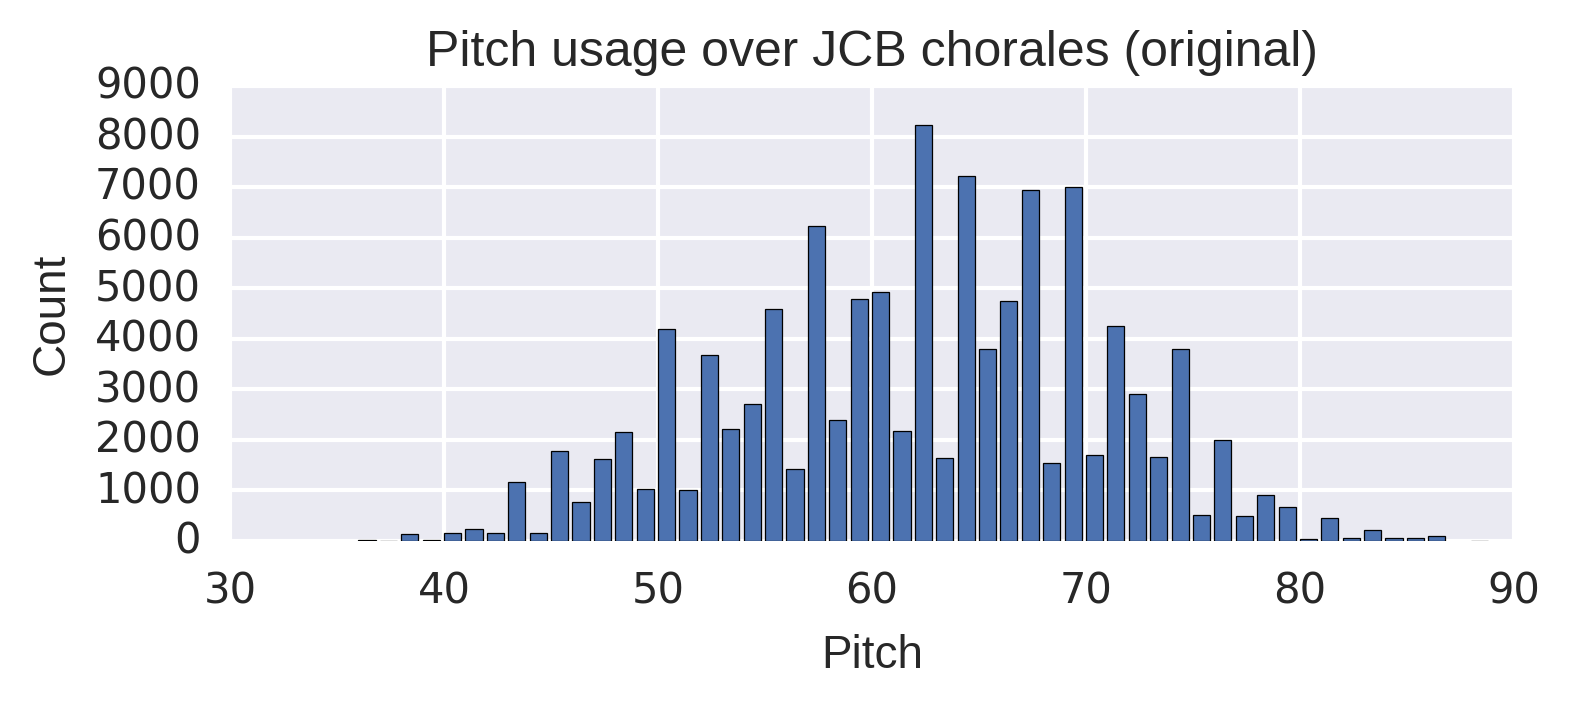
\includegraphics[width=1.0\linewidth]{pitch-usage-original.png}
    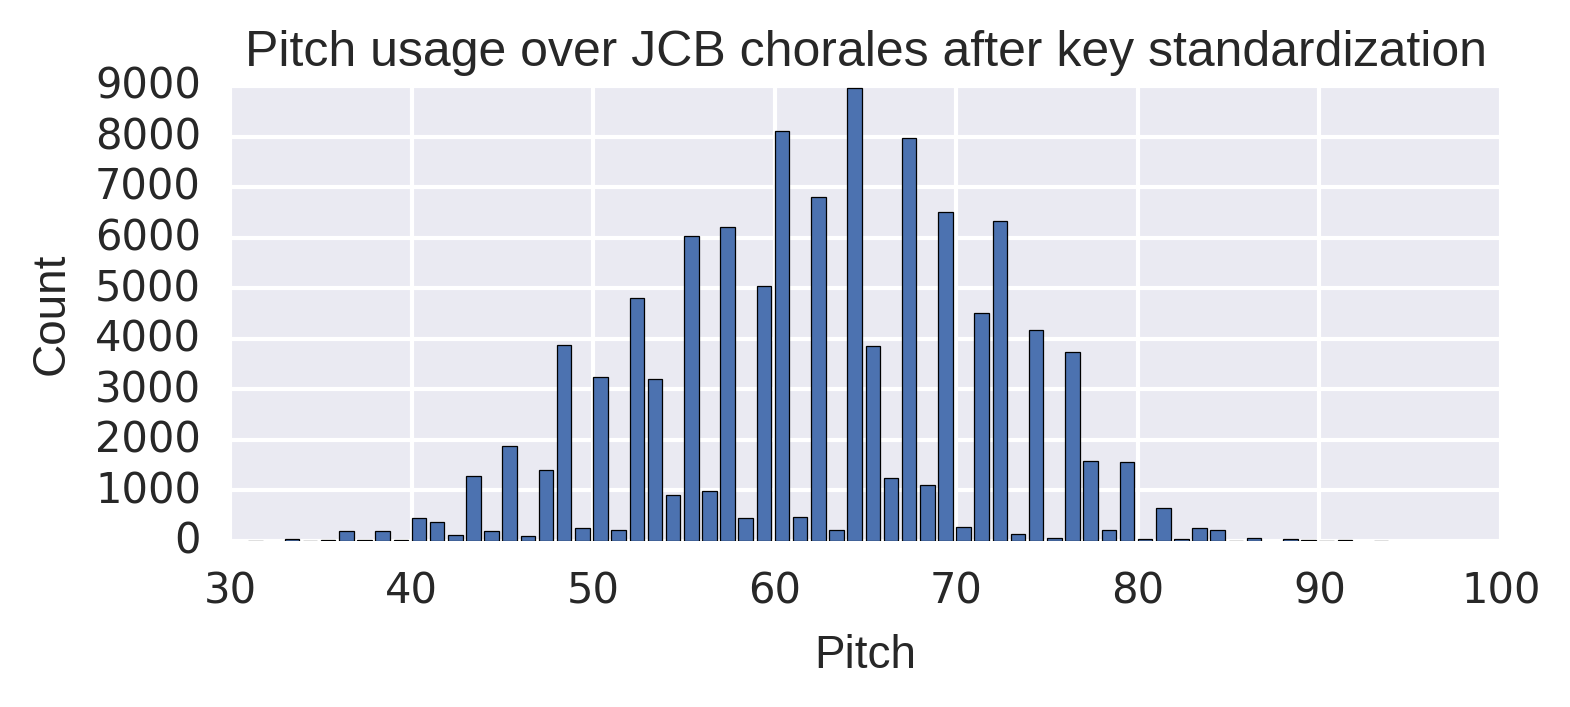
\includegraphics[width=1.0\linewidth]{pitch-usage-preproc.png}
    \caption{Pitches before and after key standardization}
    \label{fig:pitch-key-standardization}
\end{figure}

In \cref{fig:pc-key-standardization}, we visualize histograms of pitch class usages.
As expected, key normalization has increased the usage of pitch classes in the key of
C-major / A-minor (i.e. those which possess no accidentals) and decreased out of key
pitch classes (e.g. C\#, F\#).

\begin{figure}
    \centering
    \begin{subfigure}[b]{0.48\textwidth}
        \centering
        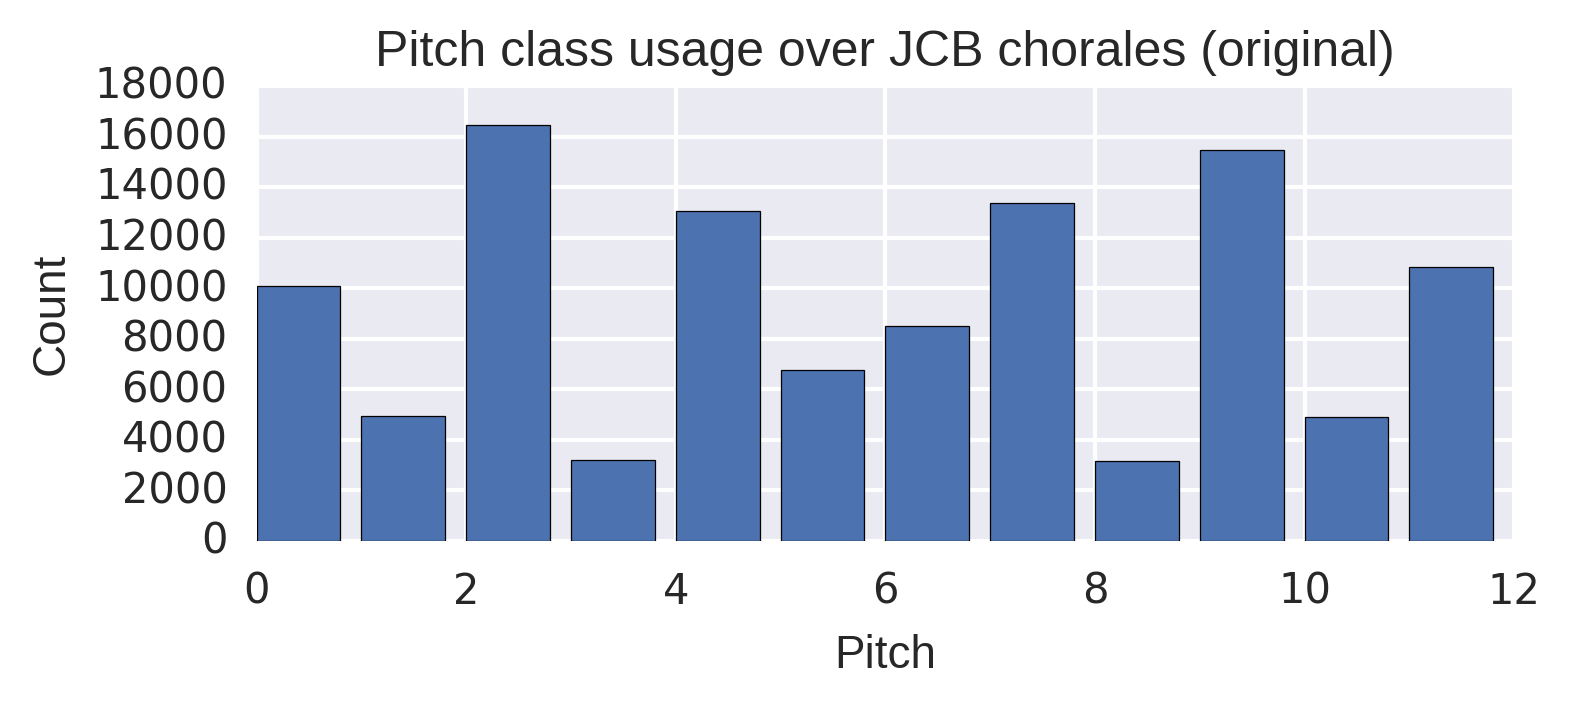
\includegraphics[width=1.0\linewidth]{pitch-class-usage-original.png}
    \end{subfigure}
    \begin{subfigure}[b]{0.48\textwidth}
        \centering
        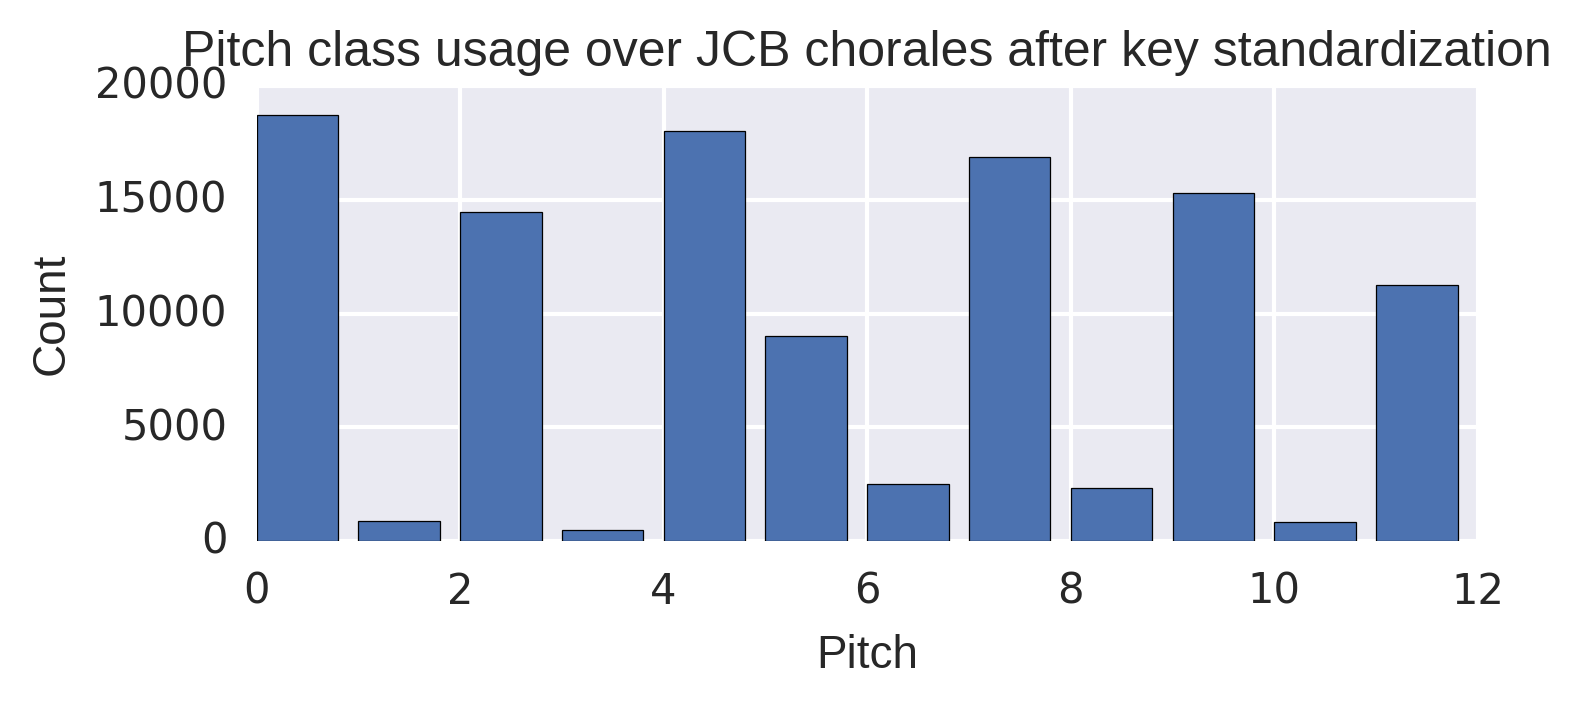
\includegraphics[width=1.0\linewidth]{pitch-class-usage-preproc.png}
    \end{subfigure}
    \caption{Pitch classes before and after key standardization}
    \label{fig:pc-key-standardization}
\end{figure}

We investigate the effects of time quantization in
\cref{fig:note-lengths-time-quantization}, which shows histograms of note
duration usages before and after quantization. \mynote{Update plots... are they affected}.

\begin{figure}[tb]
    \centering
    \begin{subfigure}[t]{0.48\textwidth}
        \centering
        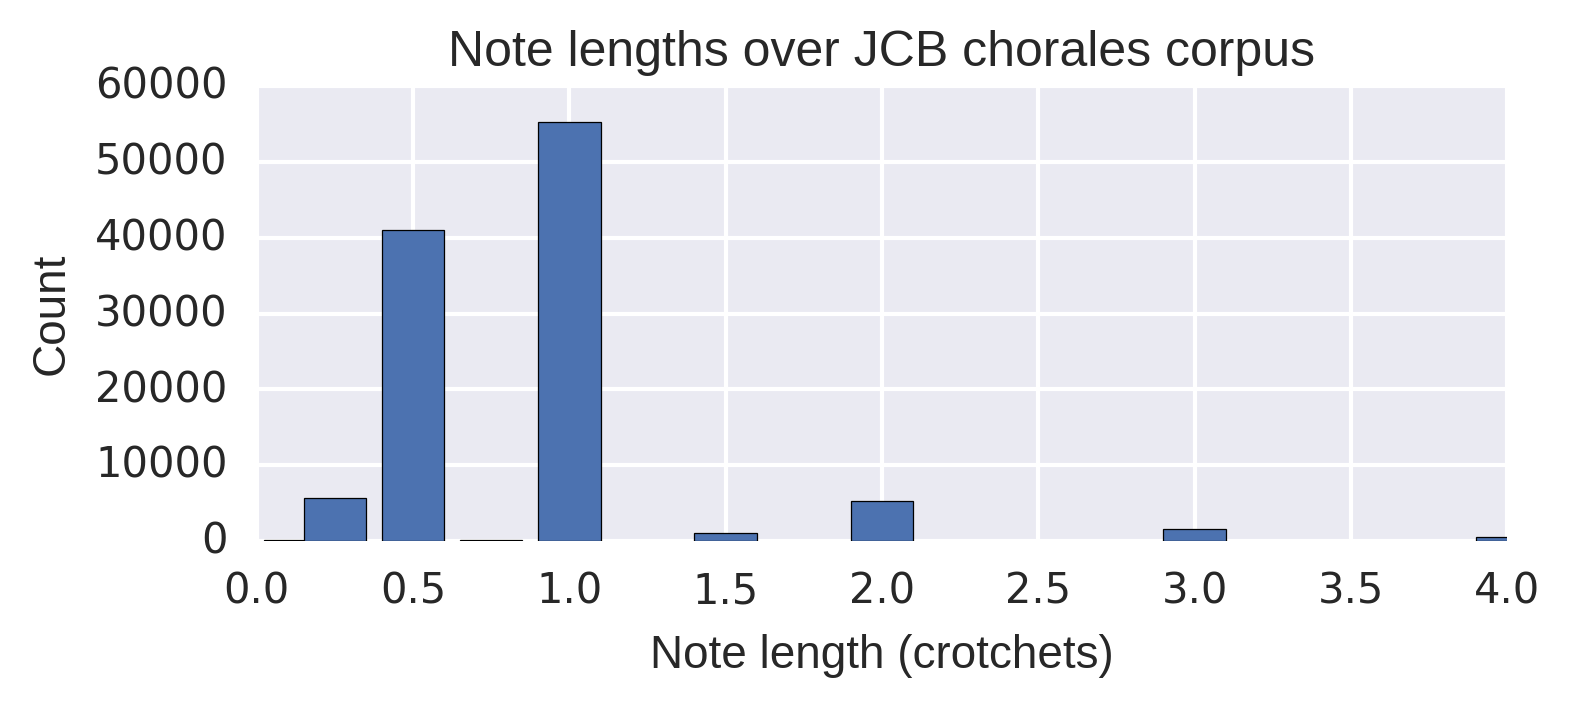
\includegraphics[width=1.0\linewidth]{note-lengths-original.png}
    \end{subfigure}
    \begin{subfigure}[t]{0.48\textwidth}
        \centering
        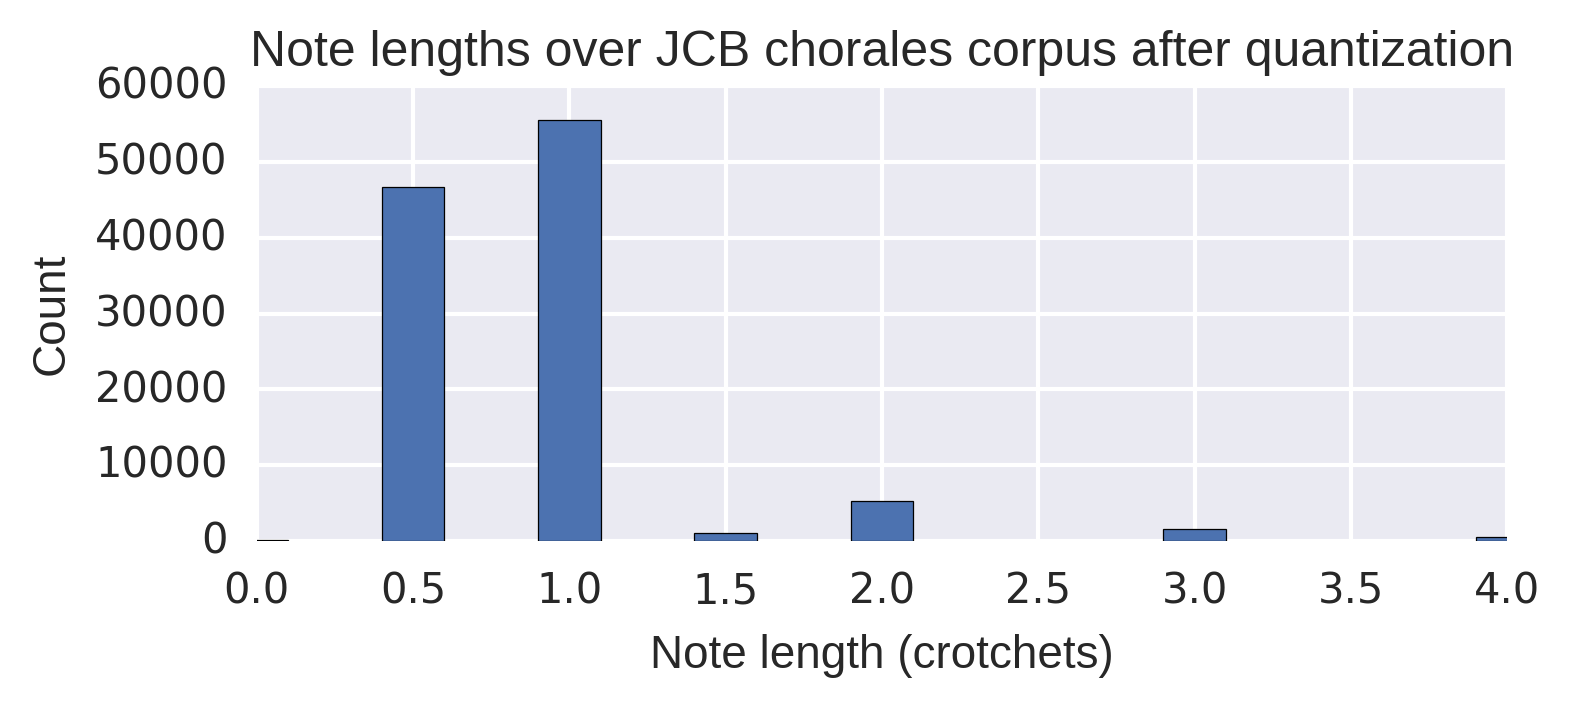
\includegraphics[width=1.0\linewidth]{note-lengths-quantized.png}
    \end{subfigure}
    \caption{Effects of time quantization on note durations}
    \label{fig:note-lengths-time-quantization}
\end{figure}

\begin{figure}[tb]
    \centering
    \begin{subfigure}[t]{0.48\textwidth}
        \centering
        %% Creator: Matplotlib, PGF backend
%%
%% To include the figure in your LaTeX document, write
%%   \input{<filename>.pgf}
%%
%% Make sure the required packages are loaded in your preamble
%%   \usepackage{pgf}
%%
%% Figures using additional raster images can only be included by \input if
%% they are in the same directory as the main LaTeX file. For loading figures
%% from other directories you can use the `import` package
%%   \usepackage{import}
%% and then include the figures with
%%   \import{<path to file>}{<filename>.pgf}
%%
%% Matplotlib used the following preamble
%%   \usepackage[utf8x]{inputenc}
%%   \usepackage[T1]{fontenc}
%%   \usepackage{fontspec}
%%
\begingroup%
\makeatletter%
\begin{pgfpicture}%
\pgfpathrectangle{\pgfpointorigin}{\pgfqpoint{4.901399in}{2.991426in}}%
\pgfusepath{use as bounding box, clip}%
\begin{pgfscope}%
\pgfsetbuttcap%
\pgfsetmiterjoin%
\definecolor{currentfill}{rgb}{1.000000,1.000000,1.000000}%
\pgfsetfillcolor{currentfill}%
\pgfsetlinewidth{0.000000pt}%
\definecolor{currentstroke}{rgb}{1.000000,1.000000,1.000000}%
\pgfsetstrokecolor{currentstroke}%
\pgfsetdash{}{0pt}%
\pgfpathmoveto{\pgfqpoint{0.000000in}{0.000000in}}%
\pgfpathlineto{\pgfqpoint{4.901399in}{0.000000in}}%
\pgfpathlineto{\pgfqpoint{4.901399in}{2.991426in}}%
\pgfpathlineto{\pgfqpoint{0.000000in}{2.991426in}}%
\pgfpathclose%
\pgfusepath{fill}%
\end{pgfscope}%
\begin{pgfscope}%
\pgfsetbuttcap%
\pgfsetmiterjoin%
\definecolor{currentfill}{rgb}{0.917647,0.917647,0.949020}%
\pgfsetfillcolor{currentfill}%
\pgfsetlinewidth{0.000000pt}%
\definecolor{currentstroke}{rgb}{0.000000,0.000000,0.000000}%
\pgfsetstrokecolor{currentstroke}%
\pgfsetstrokeopacity{0.000000}%
\pgfsetdash{}{0pt}%
\pgfpathmoveto{\pgfqpoint{0.644626in}{0.504222in}}%
\pgfpathlineto{\pgfqpoint{4.771885in}{0.504222in}}%
\pgfpathlineto{\pgfqpoint{4.771885in}{2.696981in}}%
\pgfpathlineto{\pgfqpoint{0.644626in}{2.696981in}}%
\pgfpathclose%
\pgfusepath{fill}%
\end{pgfscope}%
\begin{pgfscope}%
\pgfpathrectangle{\pgfqpoint{0.644626in}{0.504222in}}{\pgfqpoint{4.127259in}{2.192759in}} %
\pgfusepath{clip}%
\pgfsetroundcap%
\pgfsetroundjoin%
\pgfsetlinewidth{1.003750pt}%
\definecolor{currentstroke}{rgb}{1.000000,1.000000,1.000000}%
\pgfsetstrokecolor{currentstroke}%
\pgfsetdash{}{0pt}%
\pgfpathmoveto{\pgfqpoint{0.644626in}{0.504222in}}%
\pgfpathlineto{\pgfqpoint{0.644626in}{2.696981in}}%
\pgfusepath{stroke}%
\end{pgfscope}%
\begin{pgfscope}%
\pgfsetbuttcap%
\pgfsetroundjoin%
\definecolor{currentfill}{rgb}{0.501961,0.501961,0.501961}%
\pgfsetfillcolor{currentfill}%
\pgfsetlinewidth{1.003750pt}%
\definecolor{currentstroke}{rgb}{0.501961,0.501961,0.501961}%
\pgfsetstrokecolor{currentstroke}%
\pgfsetdash{}{0pt}%
\pgfsys@defobject{currentmarker}{\pgfqpoint{0.000000in}{0.000000in}}{\pgfqpoint{0.000000in}{0.000000in}}{%
\pgfpathmoveto{\pgfqpoint{0.000000in}{0.000000in}}%
\pgfpathlineto{\pgfqpoint{0.000000in}{0.000000in}}%
\pgfusepath{stroke,fill}%
}%
\begin{pgfscope}%
\pgfsys@transformshift{0.644626in}{0.504222in}%
\pgfsys@useobject{currentmarker}{}%
\end{pgfscope}%
\end{pgfscope}%
\begin{pgfscope}%
\definecolor{textcolor}{rgb}{0.150000,0.150000,0.150000}%
\pgfsetstrokecolor{textcolor}%
\pgfsetfillcolor{textcolor}%
\pgftext[x=0.644626in,y=0.407000in,,top]{\color{textcolor}\rmfamily\fontsize{8.000000}{9.600000}\selectfont \(\displaystyle 0\)}%
\end{pgfscope}%
\begin{pgfscope}%
\pgfpathrectangle{\pgfqpoint{0.644626in}{0.504222in}}{\pgfqpoint{4.127259in}{2.192759in}} %
\pgfusepath{clip}%
\pgfsetroundcap%
\pgfsetroundjoin%
\pgfsetlinewidth{1.003750pt}%
\definecolor{currentstroke}{rgb}{1.000000,1.000000,1.000000}%
\pgfsetstrokecolor{currentstroke}%
\pgfsetdash{}{0pt}%
\pgfpathmoveto{\pgfqpoint{1.676440in}{0.504222in}}%
\pgfpathlineto{\pgfqpoint{1.676440in}{2.696981in}}%
\pgfusepath{stroke}%
\end{pgfscope}%
\begin{pgfscope}%
\pgfsetbuttcap%
\pgfsetroundjoin%
\definecolor{currentfill}{rgb}{0.501961,0.501961,0.501961}%
\pgfsetfillcolor{currentfill}%
\pgfsetlinewidth{1.003750pt}%
\definecolor{currentstroke}{rgb}{0.501961,0.501961,0.501961}%
\pgfsetstrokecolor{currentstroke}%
\pgfsetdash{}{0pt}%
\pgfsys@defobject{currentmarker}{\pgfqpoint{0.000000in}{0.000000in}}{\pgfqpoint{0.000000in}{0.000000in}}{%
\pgfpathmoveto{\pgfqpoint{0.000000in}{0.000000in}}%
\pgfpathlineto{\pgfqpoint{0.000000in}{0.000000in}}%
\pgfusepath{stroke,fill}%
}%
\begin{pgfscope}%
\pgfsys@transformshift{1.676440in}{0.504222in}%
\pgfsys@useobject{currentmarker}{}%
\end{pgfscope}%
\end{pgfscope}%
\begin{pgfscope}%
\definecolor{textcolor}{rgb}{0.150000,0.150000,0.150000}%
\pgfsetstrokecolor{textcolor}%
\pgfsetfillcolor{textcolor}%
\pgftext[x=1.676440in,y=0.407000in,,top]{\color{textcolor}\rmfamily\fontsize{8.000000}{9.600000}\selectfont \(\displaystyle 1\)}%
\end{pgfscope}%
\begin{pgfscope}%
\pgfpathrectangle{\pgfqpoint{0.644626in}{0.504222in}}{\pgfqpoint{4.127259in}{2.192759in}} %
\pgfusepath{clip}%
\pgfsetroundcap%
\pgfsetroundjoin%
\pgfsetlinewidth{1.003750pt}%
\definecolor{currentstroke}{rgb}{1.000000,1.000000,1.000000}%
\pgfsetstrokecolor{currentstroke}%
\pgfsetdash{}{0pt}%
\pgfpathmoveto{\pgfqpoint{2.708255in}{0.504222in}}%
\pgfpathlineto{\pgfqpoint{2.708255in}{2.696981in}}%
\pgfusepath{stroke}%
\end{pgfscope}%
\begin{pgfscope}%
\pgfsetbuttcap%
\pgfsetroundjoin%
\definecolor{currentfill}{rgb}{0.501961,0.501961,0.501961}%
\pgfsetfillcolor{currentfill}%
\pgfsetlinewidth{1.003750pt}%
\definecolor{currentstroke}{rgb}{0.501961,0.501961,0.501961}%
\pgfsetstrokecolor{currentstroke}%
\pgfsetdash{}{0pt}%
\pgfsys@defobject{currentmarker}{\pgfqpoint{0.000000in}{0.000000in}}{\pgfqpoint{0.000000in}{0.000000in}}{%
\pgfpathmoveto{\pgfqpoint{0.000000in}{0.000000in}}%
\pgfpathlineto{\pgfqpoint{0.000000in}{0.000000in}}%
\pgfusepath{stroke,fill}%
}%
\begin{pgfscope}%
\pgfsys@transformshift{2.708255in}{0.504222in}%
\pgfsys@useobject{currentmarker}{}%
\end{pgfscope}%
\end{pgfscope}%
\begin{pgfscope}%
\definecolor{textcolor}{rgb}{0.150000,0.150000,0.150000}%
\pgfsetstrokecolor{textcolor}%
\pgfsetfillcolor{textcolor}%
\pgftext[x=2.708255in,y=0.407000in,,top]{\color{textcolor}\rmfamily\fontsize{8.000000}{9.600000}\selectfont \(\displaystyle 2\)}%
\end{pgfscope}%
\begin{pgfscope}%
\pgfpathrectangle{\pgfqpoint{0.644626in}{0.504222in}}{\pgfqpoint{4.127259in}{2.192759in}} %
\pgfusepath{clip}%
\pgfsetroundcap%
\pgfsetroundjoin%
\pgfsetlinewidth{1.003750pt}%
\definecolor{currentstroke}{rgb}{1.000000,1.000000,1.000000}%
\pgfsetstrokecolor{currentstroke}%
\pgfsetdash{}{0pt}%
\pgfpathmoveto{\pgfqpoint{3.740070in}{0.504222in}}%
\pgfpathlineto{\pgfqpoint{3.740070in}{2.696981in}}%
\pgfusepath{stroke}%
\end{pgfscope}%
\begin{pgfscope}%
\pgfsetbuttcap%
\pgfsetroundjoin%
\definecolor{currentfill}{rgb}{0.501961,0.501961,0.501961}%
\pgfsetfillcolor{currentfill}%
\pgfsetlinewidth{1.003750pt}%
\definecolor{currentstroke}{rgb}{0.501961,0.501961,0.501961}%
\pgfsetstrokecolor{currentstroke}%
\pgfsetdash{}{0pt}%
\pgfsys@defobject{currentmarker}{\pgfqpoint{0.000000in}{0.000000in}}{\pgfqpoint{0.000000in}{0.000000in}}{%
\pgfpathmoveto{\pgfqpoint{0.000000in}{0.000000in}}%
\pgfpathlineto{\pgfqpoint{0.000000in}{0.000000in}}%
\pgfusepath{stroke,fill}%
}%
\begin{pgfscope}%
\pgfsys@transformshift{3.740070in}{0.504222in}%
\pgfsys@useobject{currentmarker}{}%
\end{pgfscope}%
\end{pgfscope}%
\begin{pgfscope}%
\definecolor{textcolor}{rgb}{0.150000,0.150000,0.150000}%
\pgfsetstrokecolor{textcolor}%
\pgfsetfillcolor{textcolor}%
\pgftext[x=3.740070in,y=0.407000in,,top]{\color{textcolor}\rmfamily\fontsize{8.000000}{9.600000}\selectfont \(\displaystyle 3\)}%
\end{pgfscope}%
\begin{pgfscope}%
\pgfpathrectangle{\pgfqpoint{0.644626in}{0.504222in}}{\pgfqpoint{4.127259in}{2.192759in}} %
\pgfusepath{clip}%
\pgfsetroundcap%
\pgfsetroundjoin%
\pgfsetlinewidth{1.003750pt}%
\definecolor{currentstroke}{rgb}{1.000000,1.000000,1.000000}%
\pgfsetstrokecolor{currentstroke}%
\pgfsetdash{}{0pt}%
\pgfpathmoveto{\pgfqpoint{4.771885in}{0.504222in}}%
\pgfpathlineto{\pgfqpoint{4.771885in}{2.696981in}}%
\pgfusepath{stroke}%
\end{pgfscope}%
\begin{pgfscope}%
\pgfsetbuttcap%
\pgfsetroundjoin%
\definecolor{currentfill}{rgb}{0.501961,0.501961,0.501961}%
\pgfsetfillcolor{currentfill}%
\pgfsetlinewidth{1.003750pt}%
\definecolor{currentstroke}{rgb}{0.501961,0.501961,0.501961}%
\pgfsetstrokecolor{currentstroke}%
\pgfsetdash{}{0pt}%
\pgfsys@defobject{currentmarker}{\pgfqpoint{0.000000in}{0.000000in}}{\pgfqpoint{0.000000in}{0.000000in}}{%
\pgfpathmoveto{\pgfqpoint{0.000000in}{0.000000in}}%
\pgfpathlineto{\pgfqpoint{0.000000in}{0.000000in}}%
\pgfusepath{stroke,fill}%
}%
\begin{pgfscope}%
\pgfsys@transformshift{4.771885in}{0.504222in}%
\pgfsys@useobject{currentmarker}{}%
\end{pgfscope}%
\end{pgfscope}%
\begin{pgfscope}%
\definecolor{textcolor}{rgb}{0.150000,0.150000,0.150000}%
\pgfsetstrokecolor{textcolor}%
\pgfsetfillcolor{textcolor}%
\pgftext[x=4.771885in,y=0.407000in,,top]{\color{textcolor}\rmfamily\fontsize{8.000000}{9.600000}\selectfont \(\displaystyle 4\)}%
\end{pgfscope}%
\begin{pgfscope}%
\definecolor{textcolor}{rgb}{0.150000,0.150000,0.150000}%
\pgfsetstrokecolor{textcolor}%
\pgfsetfillcolor{textcolor}%
\pgftext[x=2.708255in,y=0.238889in,,top]{\color{textcolor}\rmfamily\fontsize{10.000000}{12.000000}\selectfont Offset from start of measure (crotchets)}%
\end{pgfscope}%
\begin{pgfscope}%
\pgfpathrectangle{\pgfqpoint{0.644626in}{0.504222in}}{\pgfqpoint{4.127259in}{2.192759in}} %
\pgfusepath{clip}%
\pgfsetroundcap%
\pgfsetroundjoin%
\pgfsetlinewidth{1.003750pt}%
\definecolor{currentstroke}{rgb}{1.000000,1.000000,1.000000}%
\pgfsetstrokecolor{currentstroke}%
\pgfsetdash{}{0pt}%
\pgfpathmoveto{\pgfqpoint{0.644626in}{0.504222in}}%
\pgfpathlineto{\pgfqpoint{4.771885in}{0.504222in}}%
\pgfusepath{stroke}%
\end{pgfscope}%
\begin{pgfscope}%
\pgfsetbuttcap%
\pgfsetroundjoin%
\definecolor{currentfill}{rgb}{0.501961,0.501961,0.501961}%
\pgfsetfillcolor{currentfill}%
\pgfsetlinewidth{1.003750pt}%
\definecolor{currentstroke}{rgb}{0.501961,0.501961,0.501961}%
\pgfsetstrokecolor{currentstroke}%
\pgfsetdash{}{0pt}%
\pgfsys@defobject{currentmarker}{\pgfqpoint{0.000000in}{0.000000in}}{\pgfqpoint{0.000000in}{0.000000in}}{%
\pgfpathmoveto{\pgfqpoint{0.000000in}{0.000000in}}%
\pgfpathlineto{\pgfqpoint{0.000000in}{0.000000in}}%
\pgfusepath{stroke,fill}%
}%
\begin{pgfscope}%
\pgfsys@transformshift{0.644626in}{0.504222in}%
\pgfsys@useobject{currentmarker}{}%
\end{pgfscope}%
\end{pgfscope}%
\begin{pgfscope}%
\definecolor{textcolor}{rgb}{0.150000,0.150000,0.150000}%
\pgfsetstrokecolor{textcolor}%
\pgfsetfillcolor{textcolor}%
\pgftext[x=0.547403in,y=0.504222in,right,]{\color{textcolor}\rmfamily\fontsize{6.000000}{7.200000}\selectfont \(\displaystyle 0\)}%
\end{pgfscope}%
\begin{pgfscope}%
\pgfpathrectangle{\pgfqpoint{0.644626in}{0.504222in}}{\pgfqpoint{4.127259in}{2.192759in}} %
\pgfusepath{clip}%
\pgfsetroundcap%
\pgfsetroundjoin%
\pgfsetlinewidth{1.003750pt}%
\definecolor{currentstroke}{rgb}{1.000000,1.000000,1.000000}%
\pgfsetstrokecolor{currentstroke}%
\pgfsetdash{}{0pt}%
\pgfpathmoveto{\pgfqpoint{0.644626in}{0.942774in}}%
\pgfpathlineto{\pgfqpoint{4.771885in}{0.942774in}}%
\pgfusepath{stroke}%
\end{pgfscope}%
\begin{pgfscope}%
\pgfsetbuttcap%
\pgfsetroundjoin%
\definecolor{currentfill}{rgb}{0.501961,0.501961,0.501961}%
\pgfsetfillcolor{currentfill}%
\pgfsetlinewidth{1.003750pt}%
\definecolor{currentstroke}{rgb}{0.501961,0.501961,0.501961}%
\pgfsetstrokecolor{currentstroke}%
\pgfsetdash{}{0pt}%
\pgfsys@defobject{currentmarker}{\pgfqpoint{0.000000in}{0.000000in}}{\pgfqpoint{0.000000in}{0.000000in}}{%
\pgfpathmoveto{\pgfqpoint{0.000000in}{0.000000in}}%
\pgfpathlineto{\pgfqpoint{0.000000in}{0.000000in}}%
\pgfusepath{stroke,fill}%
}%
\begin{pgfscope}%
\pgfsys@transformshift{0.644626in}{0.942774in}%
\pgfsys@useobject{currentmarker}{}%
\end{pgfscope}%
\end{pgfscope}%
\begin{pgfscope}%
\definecolor{textcolor}{rgb}{0.150000,0.150000,0.150000}%
\pgfsetstrokecolor{textcolor}%
\pgfsetfillcolor{textcolor}%
\pgftext[x=0.547403in,y=0.942774in,right,]{\color{textcolor}\rmfamily\fontsize{6.000000}{7.200000}\selectfont \(\displaystyle 5000\)}%
\end{pgfscope}%
\begin{pgfscope}%
\pgfpathrectangle{\pgfqpoint{0.644626in}{0.504222in}}{\pgfqpoint{4.127259in}{2.192759in}} %
\pgfusepath{clip}%
\pgfsetroundcap%
\pgfsetroundjoin%
\pgfsetlinewidth{1.003750pt}%
\definecolor{currentstroke}{rgb}{1.000000,1.000000,1.000000}%
\pgfsetstrokecolor{currentstroke}%
\pgfsetdash{}{0pt}%
\pgfpathmoveto{\pgfqpoint{0.644626in}{1.381326in}}%
\pgfpathlineto{\pgfqpoint{4.771885in}{1.381326in}}%
\pgfusepath{stroke}%
\end{pgfscope}%
\begin{pgfscope}%
\pgfsetbuttcap%
\pgfsetroundjoin%
\definecolor{currentfill}{rgb}{0.501961,0.501961,0.501961}%
\pgfsetfillcolor{currentfill}%
\pgfsetlinewidth{1.003750pt}%
\definecolor{currentstroke}{rgb}{0.501961,0.501961,0.501961}%
\pgfsetstrokecolor{currentstroke}%
\pgfsetdash{}{0pt}%
\pgfsys@defobject{currentmarker}{\pgfqpoint{0.000000in}{0.000000in}}{\pgfqpoint{0.000000in}{0.000000in}}{%
\pgfpathmoveto{\pgfqpoint{0.000000in}{0.000000in}}%
\pgfpathlineto{\pgfqpoint{0.000000in}{0.000000in}}%
\pgfusepath{stroke,fill}%
}%
\begin{pgfscope}%
\pgfsys@transformshift{0.644626in}{1.381326in}%
\pgfsys@useobject{currentmarker}{}%
\end{pgfscope}%
\end{pgfscope}%
\begin{pgfscope}%
\definecolor{textcolor}{rgb}{0.150000,0.150000,0.150000}%
\pgfsetstrokecolor{textcolor}%
\pgfsetfillcolor{textcolor}%
\pgftext[x=0.547403in,y=1.381326in,right,]{\color{textcolor}\rmfamily\fontsize{6.000000}{7.200000}\selectfont \(\displaystyle 10000\)}%
\end{pgfscope}%
\begin{pgfscope}%
\pgfpathrectangle{\pgfqpoint{0.644626in}{0.504222in}}{\pgfqpoint{4.127259in}{2.192759in}} %
\pgfusepath{clip}%
\pgfsetroundcap%
\pgfsetroundjoin%
\pgfsetlinewidth{1.003750pt}%
\definecolor{currentstroke}{rgb}{1.000000,1.000000,1.000000}%
\pgfsetstrokecolor{currentstroke}%
\pgfsetdash{}{0pt}%
\pgfpathmoveto{\pgfqpoint{0.644626in}{1.819877in}}%
\pgfpathlineto{\pgfqpoint{4.771885in}{1.819877in}}%
\pgfusepath{stroke}%
\end{pgfscope}%
\begin{pgfscope}%
\pgfsetbuttcap%
\pgfsetroundjoin%
\definecolor{currentfill}{rgb}{0.501961,0.501961,0.501961}%
\pgfsetfillcolor{currentfill}%
\pgfsetlinewidth{1.003750pt}%
\definecolor{currentstroke}{rgb}{0.501961,0.501961,0.501961}%
\pgfsetstrokecolor{currentstroke}%
\pgfsetdash{}{0pt}%
\pgfsys@defobject{currentmarker}{\pgfqpoint{0.000000in}{0.000000in}}{\pgfqpoint{0.000000in}{0.000000in}}{%
\pgfpathmoveto{\pgfqpoint{0.000000in}{0.000000in}}%
\pgfpathlineto{\pgfqpoint{0.000000in}{0.000000in}}%
\pgfusepath{stroke,fill}%
}%
\begin{pgfscope}%
\pgfsys@transformshift{0.644626in}{1.819877in}%
\pgfsys@useobject{currentmarker}{}%
\end{pgfscope}%
\end{pgfscope}%
\begin{pgfscope}%
\definecolor{textcolor}{rgb}{0.150000,0.150000,0.150000}%
\pgfsetstrokecolor{textcolor}%
\pgfsetfillcolor{textcolor}%
\pgftext[x=0.547403in,y=1.819877in,right,]{\color{textcolor}\rmfamily\fontsize{6.000000}{7.200000}\selectfont \(\displaystyle 15000\)}%
\end{pgfscope}%
\begin{pgfscope}%
\pgfpathrectangle{\pgfqpoint{0.644626in}{0.504222in}}{\pgfqpoint{4.127259in}{2.192759in}} %
\pgfusepath{clip}%
\pgfsetroundcap%
\pgfsetroundjoin%
\pgfsetlinewidth{1.003750pt}%
\definecolor{currentstroke}{rgb}{1.000000,1.000000,1.000000}%
\pgfsetstrokecolor{currentstroke}%
\pgfsetdash{}{0pt}%
\pgfpathmoveto{\pgfqpoint{0.644626in}{2.258429in}}%
\pgfpathlineto{\pgfqpoint{4.771885in}{2.258429in}}%
\pgfusepath{stroke}%
\end{pgfscope}%
\begin{pgfscope}%
\pgfsetbuttcap%
\pgfsetroundjoin%
\definecolor{currentfill}{rgb}{0.501961,0.501961,0.501961}%
\pgfsetfillcolor{currentfill}%
\pgfsetlinewidth{1.003750pt}%
\definecolor{currentstroke}{rgb}{0.501961,0.501961,0.501961}%
\pgfsetstrokecolor{currentstroke}%
\pgfsetdash{}{0pt}%
\pgfsys@defobject{currentmarker}{\pgfqpoint{0.000000in}{0.000000in}}{\pgfqpoint{0.000000in}{0.000000in}}{%
\pgfpathmoveto{\pgfqpoint{0.000000in}{0.000000in}}%
\pgfpathlineto{\pgfqpoint{0.000000in}{0.000000in}}%
\pgfusepath{stroke,fill}%
}%
\begin{pgfscope}%
\pgfsys@transformshift{0.644626in}{2.258429in}%
\pgfsys@useobject{currentmarker}{}%
\end{pgfscope}%
\end{pgfscope}%
\begin{pgfscope}%
\definecolor{textcolor}{rgb}{0.150000,0.150000,0.150000}%
\pgfsetstrokecolor{textcolor}%
\pgfsetfillcolor{textcolor}%
\pgftext[x=0.547403in,y=2.258429in,right,]{\color{textcolor}\rmfamily\fontsize{6.000000}{7.200000}\selectfont \(\displaystyle 20000\)}%
\end{pgfscope}%
\begin{pgfscope}%
\pgfpathrectangle{\pgfqpoint{0.644626in}{0.504222in}}{\pgfqpoint{4.127259in}{2.192759in}} %
\pgfusepath{clip}%
\pgfsetroundcap%
\pgfsetroundjoin%
\pgfsetlinewidth{1.003750pt}%
\definecolor{currentstroke}{rgb}{1.000000,1.000000,1.000000}%
\pgfsetstrokecolor{currentstroke}%
\pgfsetdash{}{0pt}%
\pgfpathmoveto{\pgfqpoint{0.644626in}{2.696981in}}%
\pgfpathlineto{\pgfqpoint{4.771885in}{2.696981in}}%
\pgfusepath{stroke}%
\end{pgfscope}%
\begin{pgfscope}%
\pgfsetbuttcap%
\pgfsetroundjoin%
\definecolor{currentfill}{rgb}{0.501961,0.501961,0.501961}%
\pgfsetfillcolor{currentfill}%
\pgfsetlinewidth{1.003750pt}%
\definecolor{currentstroke}{rgb}{0.501961,0.501961,0.501961}%
\pgfsetstrokecolor{currentstroke}%
\pgfsetdash{}{0pt}%
\pgfsys@defobject{currentmarker}{\pgfqpoint{0.000000in}{0.000000in}}{\pgfqpoint{0.000000in}{0.000000in}}{%
\pgfpathmoveto{\pgfqpoint{0.000000in}{0.000000in}}%
\pgfpathlineto{\pgfqpoint{0.000000in}{0.000000in}}%
\pgfusepath{stroke,fill}%
}%
\begin{pgfscope}%
\pgfsys@transformshift{0.644626in}{2.696981in}%
\pgfsys@useobject{currentmarker}{}%
\end{pgfscope}%
\end{pgfscope}%
\begin{pgfscope}%
\definecolor{textcolor}{rgb}{0.150000,0.150000,0.150000}%
\pgfsetstrokecolor{textcolor}%
\pgfsetfillcolor{textcolor}%
\pgftext[x=0.547403in,y=2.696981in,right,]{\color{textcolor}\rmfamily\fontsize{6.000000}{7.200000}\selectfont \(\displaystyle 25000\)}%
\end{pgfscope}%
\begin{pgfscope}%
\definecolor{textcolor}{rgb}{0.150000,0.150000,0.150000}%
\pgfsetstrokecolor{textcolor}%
\pgfsetfillcolor{textcolor}%
\pgftext[x=0.223333in,y=1.600601in,,bottom,rotate=90.000000]{\color{textcolor}\rmfamily\fontsize{10.000000}{12.000000}\selectfont Count}%
\end{pgfscope}%
\begin{pgfscope}%
\pgfpathrectangle{\pgfqpoint{0.644626in}{0.504222in}}{\pgfqpoint{4.127259in}{2.192759in}} %
\pgfusepath{clip}%
\pgfsetbuttcap%
\pgfsetmiterjoin%
\definecolor{currentfill}{rgb}{0.298039,0.447059,0.690196}%
\pgfsetfillcolor{currentfill}%
\pgfsetlinewidth{0.301125pt}%
\definecolor{currentstroke}{rgb}{0.000000,0.000000,0.000000}%
\pgfsetstrokecolor{currentstroke}%
\pgfsetdash{}{0pt}%
\pgfpathmoveto{\pgfqpoint{0.644626in}{0.504222in}}%
\pgfpathlineto{\pgfqpoint{0.805847in}{0.504222in}}%
\pgfpathlineto{\pgfqpoint{0.805847in}{2.432008in}}%
\pgfpathlineto{\pgfqpoint{0.644626in}{2.432008in}}%
\pgfpathclose%
\pgfusepath{stroke,fill}%
\end{pgfscope}%
\begin{pgfscope}%
\pgfpathrectangle{\pgfqpoint{0.644626in}{0.504222in}}{\pgfqpoint{4.127259in}{2.192759in}} %
\pgfusepath{clip}%
\pgfsetbuttcap%
\pgfsetmiterjoin%
\definecolor{currentfill}{rgb}{0.298039,0.447059,0.690196}%
\pgfsetfillcolor{currentfill}%
\pgfsetlinewidth{0.301125pt}%
\definecolor{currentstroke}{rgb}{0.000000,0.000000,0.000000}%
\pgfsetstrokecolor{currentstroke}%
\pgfsetdash{}{0pt}%
\pgfpathmoveto{\pgfqpoint{0.805847in}{0.504222in}}%
\pgfpathlineto{\pgfqpoint{0.967068in}{0.504222in}}%
\pgfpathlineto{\pgfqpoint{0.967068in}{0.509397in}}%
\pgfpathlineto{\pgfqpoint{0.805847in}{0.509397in}}%
\pgfpathclose%
\pgfusepath{stroke,fill}%
\end{pgfscope}%
\begin{pgfscope}%
\pgfpathrectangle{\pgfqpoint{0.644626in}{0.504222in}}{\pgfqpoint{4.127259in}{2.192759in}} %
\pgfusepath{clip}%
\pgfsetbuttcap%
\pgfsetmiterjoin%
\definecolor{currentfill}{rgb}{0.298039,0.447059,0.690196}%
\pgfsetfillcolor{currentfill}%
\pgfsetlinewidth{0.301125pt}%
\definecolor{currentstroke}{rgb}{0.000000,0.000000,0.000000}%
\pgfsetstrokecolor{currentstroke}%
\pgfsetdash{}{0pt}%
\pgfpathmoveto{\pgfqpoint{0.967068in}{0.504222in}}%
\pgfpathlineto{\pgfqpoint{1.128289in}{0.504222in}}%
\pgfpathlineto{\pgfqpoint{1.128289in}{0.504222in}}%
\pgfpathlineto{\pgfqpoint{0.967068in}{0.504222in}}%
\pgfpathclose%
\pgfusepath{stroke,fill}%
\end{pgfscope}%
\begin{pgfscope}%
\pgfpathrectangle{\pgfqpoint{0.644626in}{0.504222in}}{\pgfqpoint{4.127259in}{2.192759in}} %
\pgfusepath{clip}%
\pgfsetbuttcap%
\pgfsetmiterjoin%
\definecolor{currentfill}{rgb}{0.298039,0.447059,0.690196}%
\pgfsetfillcolor{currentfill}%
\pgfsetlinewidth{0.301125pt}%
\definecolor{currentstroke}{rgb}{0.000000,0.000000,0.000000}%
\pgfsetstrokecolor{currentstroke}%
\pgfsetdash{}{0pt}%
\pgfpathmoveto{\pgfqpoint{1.128289in}{0.504222in}}%
\pgfpathlineto{\pgfqpoint{1.289510in}{0.504222in}}%
\pgfpathlineto{\pgfqpoint{1.289510in}{0.961807in}}%
\pgfpathlineto{\pgfqpoint{1.128289in}{0.961807in}}%
\pgfpathclose%
\pgfusepath{stroke,fill}%
\end{pgfscope}%
\begin{pgfscope}%
\pgfpathrectangle{\pgfqpoint{0.644626in}{0.504222in}}{\pgfqpoint{4.127259in}{2.192759in}} %
\pgfusepath{clip}%
\pgfsetbuttcap%
\pgfsetmiterjoin%
\definecolor{currentfill}{rgb}{0.298039,0.447059,0.690196}%
\pgfsetfillcolor{currentfill}%
\pgfsetlinewidth{0.301125pt}%
\definecolor{currentstroke}{rgb}{0.000000,0.000000,0.000000}%
\pgfsetstrokecolor{currentstroke}%
\pgfsetdash{}{0pt}%
\pgfpathmoveto{\pgfqpoint{1.289510in}{0.504222in}}%
\pgfpathlineto{\pgfqpoint{1.450731in}{0.504222in}}%
\pgfpathlineto{\pgfqpoint{1.450731in}{0.536412in}}%
\pgfpathlineto{\pgfqpoint{1.289510in}{0.536412in}}%
\pgfpathclose%
\pgfusepath{stroke,fill}%
\end{pgfscope}%
\begin{pgfscope}%
\pgfpathrectangle{\pgfqpoint{0.644626in}{0.504222in}}{\pgfqpoint{4.127259in}{2.192759in}} %
\pgfusepath{clip}%
\pgfsetbuttcap%
\pgfsetmiterjoin%
\definecolor{currentfill}{rgb}{0.298039,0.447059,0.690196}%
\pgfsetfillcolor{currentfill}%
\pgfsetlinewidth{0.301125pt}%
\definecolor{currentstroke}{rgb}{0.000000,0.000000,0.000000}%
\pgfsetstrokecolor{currentstroke}%
\pgfsetdash{}{0pt}%
\pgfpathmoveto{\pgfqpoint{1.450731in}{0.504222in}}%
\pgfpathlineto{\pgfqpoint{1.611952in}{0.504222in}}%
\pgfpathlineto{\pgfqpoint{1.611952in}{0.504485in}}%
\pgfpathlineto{\pgfqpoint{1.450731in}{0.504485in}}%
\pgfpathclose%
\pgfusepath{stroke,fill}%
\end{pgfscope}%
\begin{pgfscope}%
\pgfpathrectangle{\pgfqpoint{0.644626in}{0.504222in}}{\pgfqpoint{4.127259in}{2.192759in}} %
\pgfusepath{clip}%
\pgfsetbuttcap%
\pgfsetmiterjoin%
\definecolor{currentfill}{rgb}{0.298039,0.447059,0.690196}%
\pgfsetfillcolor{currentfill}%
\pgfsetlinewidth{0.301125pt}%
\definecolor{currentstroke}{rgb}{0.000000,0.000000,0.000000}%
\pgfsetstrokecolor{currentstroke}%
\pgfsetdash{}{0pt}%
\pgfpathmoveto{\pgfqpoint{1.611952in}{0.504222in}}%
\pgfpathlineto{\pgfqpoint{1.773173in}{0.504222in}}%
\pgfpathlineto{\pgfqpoint{1.773173in}{2.018629in}}%
\pgfpathlineto{\pgfqpoint{1.611952in}{2.018629in}}%
\pgfpathclose%
\pgfusepath{stroke,fill}%
\end{pgfscope}%
\begin{pgfscope}%
\pgfpathrectangle{\pgfqpoint{0.644626in}{0.504222in}}{\pgfqpoint{4.127259in}{2.192759in}} %
\pgfusepath{clip}%
\pgfsetbuttcap%
\pgfsetmiterjoin%
\definecolor{currentfill}{rgb}{0.298039,0.447059,0.690196}%
\pgfsetfillcolor{currentfill}%
\pgfsetlinewidth{0.301125pt}%
\definecolor{currentstroke}{rgb}{0.000000,0.000000,0.000000}%
\pgfsetstrokecolor{currentstroke}%
\pgfsetdash{}{0pt}%
\pgfpathmoveto{\pgfqpoint{1.773173in}{0.504222in}}%
\pgfpathlineto{\pgfqpoint{1.934394in}{0.504222in}}%
\pgfpathlineto{\pgfqpoint{1.934394in}{0.504222in}}%
\pgfpathlineto{\pgfqpoint{1.773173in}{0.504222in}}%
\pgfpathclose%
\pgfusepath{stroke,fill}%
\end{pgfscope}%
\begin{pgfscope}%
\pgfpathrectangle{\pgfqpoint{0.644626in}{0.504222in}}{\pgfqpoint{4.127259in}{2.192759in}} %
\pgfusepath{clip}%
\pgfsetbuttcap%
\pgfsetmiterjoin%
\definecolor{currentfill}{rgb}{0.298039,0.447059,0.690196}%
\pgfsetfillcolor{currentfill}%
\pgfsetlinewidth{0.301125pt}%
\definecolor{currentstroke}{rgb}{0.000000,0.000000,0.000000}%
\pgfsetstrokecolor{currentstroke}%
\pgfsetdash{}{0pt}%
\pgfpathmoveto{\pgfqpoint{1.934394in}{0.504222in}}%
\pgfpathlineto{\pgfqpoint{2.095615in}{0.504222in}}%
\pgfpathlineto{\pgfqpoint{2.095615in}{0.509572in}}%
\pgfpathlineto{\pgfqpoint{1.934394in}{0.509572in}}%
\pgfpathclose%
\pgfusepath{stroke,fill}%
\end{pgfscope}%
\begin{pgfscope}%
\pgfpathrectangle{\pgfqpoint{0.644626in}{0.504222in}}{\pgfqpoint{4.127259in}{2.192759in}} %
\pgfusepath{clip}%
\pgfsetbuttcap%
\pgfsetmiterjoin%
\definecolor{currentfill}{rgb}{0.298039,0.447059,0.690196}%
\pgfsetfillcolor{currentfill}%
\pgfsetlinewidth{0.301125pt}%
\definecolor{currentstroke}{rgb}{0.000000,0.000000,0.000000}%
\pgfsetstrokecolor{currentstroke}%
\pgfsetdash{}{0pt}%
\pgfpathmoveto{\pgfqpoint{2.095615in}{0.504222in}}%
\pgfpathlineto{\pgfqpoint{2.256836in}{0.504222in}}%
\pgfpathlineto{\pgfqpoint{2.256836in}{0.979524in}}%
\pgfpathlineto{\pgfqpoint{2.095615in}{0.979524in}}%
\pgfpathclose%
\pgfusepath{stroke,fill}%
\end{pgfscope}%
\begin{pgfscope}%
\pgfpathrectangle{\pgfqpoint{0.644626in}{0.504222in}}{\pgfqpoint{4.127259in}{2.192759in}} %
\pgfusepath{clip}%
\pgfsetbuttcap%
\pgfsetmiterjoin%
\definecolor{currentfill}{rgb}{0.298039,0.447059,0.690196}%
\pgfsetfillcolor{currentfill}%
\pgfsetlinewidth{0.301125pt}%
\definecolor{currentstroke}{rgb}{0.000000,0.000000,0.000000}%
\pgfsetstrokecolor{currentstroke}%
\pgfsetdash{}{0pt}%
\pgfpathmoveto{\pgfqpoint{2.256836in}{0.504222in}}%
\pgfpathlineto{\pgfqpoint{2.418057in}{0.504222in}}%
\pgfpathlineto{\pgfqpoint{2.418057in}{0.504222in}}%
\pgfpathlineto{\pgfqpoint{2.256836in}{0.504222in}}%
\pgfpathclose%
\pgfusepath{stroke,fill}%
\end{pgfscope}%
\begin{pgfscope}%
\pgfpathrectangle{\pgfqpoint{0.644626in}{0.504222in}}{\pgfqpoint{4.127259in}{2.192759in}} %
\pgfusepath{clip}%
\pgfsetbuttcap%
\pgfsetmiterjoin%
\definecolor{currentfill}{rgb}{0.298039,0.447059,0.690196}%
\pgfsetfillcolor{currentfill}%
\pgfsetlinewidth{0.301125pt}%
\definecolor{currentstroke}{rgb}{0.000000,0.000000,0.000000}%
\pgfsetstrokecolor{currentstroke}%
\pgfsetdash{}{0pt}%
\pgfpathmoveto{\pgfqpoint{2.418057in}{0.504222in}}%
\pgfpathlineto{\pgfqpoint{2.579278in}{0.504222in}}%
\pgfpathlineto{\pgfqpoint{2.579278in}{0.537289in}}%
\pgfpathlineto{\pgfqpoint{2.418057in}{0.537289in}}%
\pgfpathclose%
\pgfusepath{stroke,fill}%
\end{pgfscope}%
\begin{pgfscope}%
\pgfpathrectangle{\pgfqpoint{0.644626in}{0.504222in}}{\pgfqpoint{4.127259in}{2.192759in}} %
\pgfusepath{clip}%
\pgfsetbuttcap%
\pgfsetmiterjoin%
\definecolor{currentfill}{rgb}{0.298039,0.447059,0.690196}%
\pgfsetfillcolor{currentfill}%
\pgfsetlinewidth{0.301125pt}%
\definecolor{currentstroke}{rgb}{0.000000,0.000000,0.000000}%
\pgfsetstrokecolor{currentstroke}%
\pgfsetdash{}{0pt}%
\pgfpathmoveto{\pgfqpoint{2.579278in}{0.504222in}}%
\pgfpathlineto{\pgfqpoint{2.740499in}{0.504222in}}%
\pgfpathlineto{\pgfqpoint{2.740499in}{2.242291in}}%
\pgfpathlineto{\pgfqpoint{2.579278in}{2.242291in}}%
\pgfpathclose%
\pgfusepath{stroke,fill}%
\end{pgfscope}%
\begin{pgfscope}%
\pgfpathrectangle{\pgfqpoint{0.644626in}{0.504222in}}{\pgfqpoint{4.127259in}{2.192759in}} %
\pgfusepath{clip}%
\pgfsetbuttcap%
\pgfsetmiterjoin%
\definecolor{currentfill}{rgb}{0.298039,0.447059,0.690196}%
\pgfsetfillcolor{currentfill}%
\pgfsetlinewidth{0.301125pt}%
\definecolor{currentstroke}{rgb}{0.000000,0.000000,0.000000}%
\pgfsetstrokecolor{currentstroke}%
\pgfsetdash{}{0pt}%
\pgfpathmoveto{\pgfqpoint{2.740499in}{0.504222in}}%
\pgfpathlineto{\pgfqpoint{2.901720in}{0.504222in}}%
\pgfpathlineto{\pgfqpoint{2.901720in}{0.504222in}}%
\pgfpathlineto{\pgfqpoint{2.740499in}{0.504222in}}%
\pgfpathclose%
\pgfusepath{stroke,fill}%
\end{pgfscope}%
\begin{pgfscope}%
\pgfpathrectangle{\pgfqpoint{0.644626in}{0.504222in}}{\pgfqpoint{4.127259in}{2.192759in}} %
\pgfusepath{clip}%
\pgfsetbuttcap%
\pgfsetmiterjoin%
\definecolor{currentfill}{rgb}{0.298039,0.447059,0.690196}%
\pgfsetfillcolor{currentfill}%
\pgfsetlinewidth{0.301125pt}%
\definecolor{currentstroke}{rgb}{0.000000,0.000000,0.000000}%
\pgfsetstrokecolor{currentstroke}%
\pgfsetdash{}{0pt}%
\pgfpathmoveto{\pgfqpoint{2.901720in}{0.504222in}}%
\pgfpathlineto{\pgfqpoint{3.062942in}{0.504222in}}%
\pgfpathlineto{\pgfqpoint{3.062942in}{0.505537in}}%
\pgfpathlineto{\pgfqpoint{2.901720in}{0.505537in}}%
\pgfpathclose%
\pgfusepath{stroke,fill}%
\end{pgfscope}%
\begin{pgfscope}%
\pgfpathrectangle{\pgfqpoint{0.644626in}{0.504222in}}{\pgfqpoint{4.127259in}{2.192759in}} %
\pgfusepath{clip}%
\pgfsetbuttcap%
\pgfsetmiterjoin%
\definecolor{currentfill}{rgb}{0.298039,0.447059,0.690196}%
\pgfsetfillcolor{currentfill}%
\pgfsetlinewidth{0.301125pt}%
\definecolor{currentstroke}{rgb}{0.000000,0.000000,0.000000}%
\pgfsetstrokecolor{currentstroke}%
\pgfsetdash{}{0pt}%
\pgfpathmoveto{\pgfqpoint{3.062942in}{0.504222in}}%
\pgfpathlineto{\pgfqpoint{3.224163in}{0.504222in}}%
\pgfpathlineto{\pgfqpoint{3.224163in}{0.504222in}}%
\pgfpathlineto{\pgfqpoint{3.062942in}{0.504222in}}%
\pgfpathclose%
\pgfusepath{stroke,fill}%
\end{pgfscope}%
\begin{pgfscope}%
\pgfpathrectangle{\pgfqpoint{0.644626in}{0.504222in}}{\pgfqpoint{4.127259in}{2.192759in}} %
\pgfusepath{clip}%
\pgfsetbuttcap%
\pgfsetmiterjoin%
\definecolor{currentfill}{rgb}{0.298039,0.447059,0.690196}%
\pgfsetfillcolor{currentfill}%
\pgfsetlinewidth{0.301125pt}%
\definecolor{currentstroke}{rgb}{0.000000,0.000000,0.000000}%
\pgfsetstrokecolor{currentstroke}%
\pgfsetdash{}{0pt}%
\pgfpathmoveto{\pgfqpoint{3.224163in}{0.504222in}}%
\pgfpathlineto{\pgfqpoint{3.385384in}{0.504222in}}%
\pgfpathlineto{\pgfqpoint{3.385384in}{0.846029in}}%
\pgfpathlineto{\pgfqpoint{3.224163in}{0.846029in}}%
\pgfpathclose%
\pgfusepath{stroke,fill}%
\end{pgfscope}%
\begin{pgfscope}%
\pgfpathrectangle{\pgfqpoint{0.644626in}{0.504222in}}{\pgfqpoint{4.127259in}{2.192759in}} %
\pgfusepath{clip}%
\pgfsetbuttcap%
\pgfsetmiterjoin%
\definecolor{currentfill}{rgb}{0.298039,0.447059,0.690196}%
\pgfsetfillcolor{currentfill}%
\pgfsetlinewidth{0.301125pt}%
\definecolor{currentstroke}{rgb}{0.000000,0.000000,0.000000}%
\pgfsetstrokecolor{currentstroke}%
\pgfsetdash{}{0pt}%
\pgfpathmoveto{\pgfqpoint{3.385384in}{0.504222in}}%
\pgfpathlineto{\pgfqpoint{3.546605in}{0.504222in}}%
\pgfpathlineto{\pgfqpoint{3.546605in}{0.526851in}}%
\pgfpathlineto{\pgfqpoint{3.385384in}{0.526851in}}%
\pgfpathclose%
\pgfusepath{stroke,fill}%
\end{pgfscope}%
\begin{pgfscope}%
\pgfpathrectangle{\pgfqpoint{0.644626in}{0.504222in}}{\pgfqpoint{4.127259in}{2.192759in}} %
\pgfusepath{clip}%
\pgfsetbuttcap%
\pgfsetmiterjoin%
\definecolor{currentfill}{rgb}{0.298039,0.447059,0.690196}%
\pgfsetfillcolor{currentfill}%
\pgfsetlinewidth{0.301125pt}%
\definecolor{currentstroke}{rgb}{0.000000,0.000000,0.000000}%
\pgfsetstrokecolor{currentstroke}%
\pgfsetdash{}{0pt}%
\pgfpathmoveto{\pgfqpoint{3.546605in}{0.504222in}}%
\pgfpathlineto{\pgfqpoint{3.707826in}{0.504222in}}%
\pgfpathlineto{\pgfqpoint{3.707826in}{0.504573in}}%
\pgfpathlineto{\pgfqpoint{3.546605in}{0.504573in}}%
\pgfpathclose%
\pgfusepath{stroke,fill}%
\end{pgfscope}%
\begin{pgfscope}%
\pgfpathrectangle{\pgfqpoint{0.644626in}{0.504222in}}{\pgfqpoint{4.127259in}{2.192759in}} %
\pgfusepath{clip}%
\pgfsetbuttcap%
\pgfsetmiterjoin%
\definecolor{currentfill}{rgb}{0.298039,0.447059,0.690196}%
\pgfsetfillcolor{currentfill}%
\pgfsetlinewidth{0.301125pt}%
\definecolor{currentstroke}{rgb}{0.000000,0.000000,0.000000}%
\pgfsetstrokecolor{currentstroke}%
\pgfsetdash{}{0pt}%
\pgfpathmoveto{\pgfqpoint{3.707826in}{0.504222in}}%
\pgfpathlineto{\pgfqpoint{3.869047in}{0.504222in}}%
\pgfpathlineto{\pgfqpoint{3.869047in}{2.140810in}}%
\pgfpathlineto{\pgfqpoint{3.707826in}{2.140810in}}%
\pgfpathclose%
\pgfusepath{stroke,fill}%
\end{pgfscope}%
\begin{pgfscope}%
\pgfpathrectangle{\pgfqpoint{0.644626in}{0.504222in}}{\pgfqpoint{4.127259in}{2.192759in}} %
\pgfusepath{clip}%
\pgfsetbuttcap%
\pgfsetmiterjoin%
\definecolor{currentfill}{rgb}{0.298039,0.447059,0.690196}%
\pgfsetfillcolor{currentfill}%
\pgfsetlinewidth{0.301125pt}%
\definecolor{currentstroke}{rgb}{0.000000,0.000000,0.000000}%
\pgfsetstrokecolor{currentstroke}%
\pgfsetdash{}{0pt}%
\pgfpathmoveto{\pgfqpoint{3.869047in}{0.504222in}}%
\pgfpathlineto{\pgfqpoint{4.030268in}{0.504222in}}%
\pgfpathlineto{\pgfqpoint{4.030268in}{0.507204in}}%
\pgfpathlineto{\pgfqpoint{3.869047in}{0.507204in}}%
\pgfpathclose%
\pgfusepath{stroke,fill}%
\end{pgfscope}%
\begin{pgfscope}%
\pgfpathrectangle{\pgfqpoint{0.644626in}{0.504222in}}{\pgfqpoint{4.127259in}{2.192759in}} %
\pgfusepath{clip}%
\pgfsetbuttcap%
\pgfsetmiterjoin%
\definecolor{currentfill}{rgb}{0.298039,0.447059,0.690196}%
\pgfsetfillcolor{currentfill}%
\pgfsetlinewidth{0.301125pt}%
\definecolor{currentstroke}{rgb}{0.000000,0.000000,0.000000}%
\pgfsetstrokecolor{currentstroke}%
\pgfsetdash{}{0pt}%
\pgfpathmoveto{\pgfqpoint{4.030268in}{0.504222in}}%
\pgfpathlineto{\pgfqpoint{4.191489in}{0.504222in}}%
\pgfpathlineto{\pgfqpoint{4.191489in}{0.504222in}}%
\pgfpathlineto{\pgfqpoint{4.030268in}{0.504222in}}%
\pgfpathclose%
\pgfusepath{stroke,fill}%
\end{pgfscope}%
\begin{pgfscope}%
\pgfpathrectangle{\pgfqpoint{0.644626in}{0.504222in}}{\pgfqpoint{4.127259in}{2.192759in}} %
\pgfusepath{clip}%
\pgfsetbuttcap%
\pgfsetmiterjoin%
\definecolor{currentfill}{rgb}{0.298039,0.447059,0.690196}%
\pgfsetfillcolor{currentfill}%
\pgfsetlinewidth{0.301125pt}%
\definecolor{currentstroke}{rgb}{0.000000,0.000000,0.000000}%
\pgfsetstrokecolor{currentstroke}%
\pgfsetdash{}{0pt}%
\pgfpathmoveto{\pgfqpoint{4.191489in}{0.504222in}}%
\pgfpathlineto{\pgfqpoint{4.352710in}{0.504222in}}%
\pgfpathlineto{\pgfqpoint{4.352710in}{0.940756in}}%
\pgfpathlineto{\pgfqpoint{4.191489in}{0.940756in}}%
\pgfpathclose%
\pgfusepath{stroke,fill}%
\end{pgfscope}%
\begin{pgfscope}%
\pgfpathrectangle{\pgfqpoint{0.644626in}{0.504222in}}{\pgfqpoint{4.127259in}{2.192759in}} %
\pgfusepath{clip}%
\pgfsetbuttcap%
\pgfsetmiterjoin%
\definecolor{currentfill}{rgb}{0.298039,0.447059,0.690196}%
\pgfsetfillcolor{currentfill}%
\pgfsetlinewidth{0.301125pt}%
\definecolor{currentstroke}{rgb}{0.000000,0.000000,0.000000}%
\pgfsetstrokecolor{currentstroke}%
\pgfsetdash{}{0pt}%
\pgfpathmoveto{\pgfqpoint{4.352710in}{0.504222in}}%
\pgfpathlineto{\pgfqpoint{4.513931in}{0.504222in}}%
\pgfpathlineto{\pgfqpoint{4.513931in}{0.504222in}}%
\pgfpathlineto{\pgfqpoint{4.352710in}{0.504222in}}%
\pgfpathclose%
\pgfusepath{stroke,fill}%
\end{pgfscope}%
\begin{pgfscope}%
\pgfpathrectangle{\pgfqpoint{0.644626in}{0.504222in}}{\pgfqpoint{4.127259in}{2.192759in}} %
\pgfusepath{clip}%
\pgfsetbuttcap%
\pgfsetmiterjoin%
\definecolor{currentfill}{rgb}{0.298039,0.447059,0.690196}%
\pgfsetfillcolor{currentfill}%
\pgfsetlinewidth{0.301125pt}%
\definecolor{currentstroke}{rgb}{0.000000,0.000000,0.000000}%
\pgfsetstrokecolor{currentstroke}%
\pgfsetdash{}{0pt}%
\pgfpathmoveto{\pgfqpoint{4.513931in}{0.504222in}}%
\pgfpathlineto{\pgfqpoint{4.675152in}{0.504222in}}%
\pgfpathlineto{\pgfqpoint{4.675152in}{0.524571in}}%
\pgfpathlineto{\pgfqpoint{4.513931in}{0.524571in}}%
\pgfpathclose%
\pgfusepath{stroke,fill}%
\end{pgfscope}%
\begin{pgfscope}%
\pgfpathrectangle{\pgfqpoint{0.644626in}{0.504222in}}{\pgfqpoint{4.127259in}{2.192759in}} %
\pgfusepath{clip}%
\pgfsetbuttcap%
\pgfsetmiterjoin%
\definecolor{currentfill}{rgb}{0.298039,0.447059,0.690196}%
\pgfsetfillcolor{currentfill}%
\pgfsetlinewidth{0.301125pt}%
\definecolor{currentstroke}{rgb}{0.000000,0.000000,0.000000}%
\pgfsetstrokecolor{currentstroke}%
\pgfsetdash{}{0pt}%
\pgfpathmoveto{\pgfqpoint{4.675152in}{0.504222in}}%
\pgfpathlineto{\pgfqpoint{4.836373in}{0.504222in}}%
\pgfpathlineto{\pgfqpoint{4.836373in}{0.504222in}}%
\pgfpathlineto{\pgfqpoint{4.675152in}{0.504222in}}%
\pgfpathclose%
\pgfusepath{stroke,fill}%
\end{pgfscope}%
\begin{pgfscope}%
\pgfpathrectangle{\pgfqpoint{0.644626in}{0.504222in}}{\pgfqpoint{4.127259in}{2.192759in}} %
\pgfusepath{clip}%
\pgfsetbuttcap%
\pgfsetmiterjoin%
\definecolor{currentfill}{rgb}{0.298039,0.447059,0.690196}%
\pgfsetfillcolor{currentfill}%
\pgfsetlinewidth{0.301125pt}%
\definecolor{currentstroke}{rgb}{0.000000,0.000000,0.000000}%
\pgfsetstrokecolor{currentstroke}%
\pgfsetdash{}{0pt}%
\pgfpathmoveto{\pgfqpoint{4.836373in}{0.504222in}}%
\pgfpathlineto{\pgfqpoint{4.997594in}{0.504222in}}%
\pgfpathlineto{\pgfqpoint{4.997594in}{0.504222in}}%
\pgfpathlineto{\pgfqpoint{4.836373in}{0.504222in}}%
\pgfpathclose%
\pgfusepath{stroke,fill}%
\end{pgfscope}%
\begin{pgfscope}%
\pgfpathrectangle{\pgfqpoint{0.644626in}{0.504222in}}{\pgfqpoint{4.127259in}{2.192759in}} %
\pgfusepath{clip}%
\pgfsetbuttcap%
\pgfsetmiterjoin%
\definecolor{currentfill}{rgb}{0.298039,0.447059,0.690196}%
\pgfsetfillcolor{currentfill}%
\pgfsetlinewidth{0.301125pt}%
\definecolor{currentstroke}{rgb}{0.000000,0.000000,0.000000}%
\pgfsetstrokecolor{currentstroke}%
\pgfsetdash{}{0pt}%
\pgfpathmoveto{\pgfqpoint{4.997594in}{0.504222in}}%
\pgfpathlineto{\pgfqpoint{5.158815in}{0.504222in}}%
\pgfpathlineto{\pgfqpoint{5.158815in}{0.504222in}}%
\pgfpathlineto{\pgfqpoint{4.997594in}{0.504222in}}%
\pgfpathclose%
\pgfusepath{stroke,fill}%
\end{pgfscope}%
\begin{pgfscope}%
\pgfpathrectangle{\pgfqpoint{0.644626in}{0.504222in}}{\pgfqpoint{4.127259in}{2.192759in}} %
\pgfusepath{clip}%
\pgfsetbuttcap%
\pgfsetmiterjoin%
\definecolor{currentfill}{rgb}{0.298039,0.447059,0.690196}%
\pgfsetfillcolor{currentfill}%
\pgfsetlinewidth{0.301125pt}%
\definecolor{currentstroke}{rgb}{0.000000,0.000000,0.000000}%
\pgfsetstrokecolor{currentstroke}%
\pgfsetdash{}{0pt}%
\pgfpathmoveto{\pgfqpoint{5.158815in}{0.504222in}}%
\pgfpathlineto{\pgfqpoint{5.320036in}{0.504222in}}%
\pgfpathlineto{\pgfqpoint{5.320036in}{0.504222in}}%
\pgfpathlineto{\pgfqpoint{5.158815in}{0.504222in}}%
\pgfpathclose%
\pgfusepath{stroke,fill}%
\end{pgfscope}%
\begin{pgfscope}%
\pgfpathrectangle{\pgfqpoint{0.644626in}{0.504222in}}{\pgfqpoint{4.127259in}{2.192759in}} %
\pgfusepath{clip}%
\pgfsetbuttcap%
\pgfsetmiterjoin%
\definecolor{currentfill}{rgb}{0.298039,0.447059,0.690196}%
\pgfsetfillcolor{currentfill}%
\pgfsetlinewidth{0.301125pt}%
\definecolor{currentstroke}{rgb}{0.000000,0.000000,0.000000}%
\pgfsetstrokecolor{currentstroke}%
\pgfsetdash{}{0pt}%
\pgfpathmoveto{\pgfqpoint{5.320036in}{0.504222in}}%
\pgfpathlineto{\pgfqpoint{5.481258in}{0.504222in}}%
\pgfpathlineto{\pgfqpoint{5.481258in}{0.504222in}}%
\pgfpathlineto{\pgfqpoint{5.320036in}{0.504222in}}%
\pgfpathclose%
\pgfusepath{stroke,fill}%
\end{pgfscope}%
\begin{pgfscope}%
\pgfpathrectangle{\pgfqpoint{0.644626in}{0.504222in}}{\pgfqpoint{4.127259in}{2.192759in}} %
\pgfusepath{clip}%
\pgfsetbuttcap%
\pgfsetmiterjoin%
\definecolor{currentfill}{rgb}{0.298039,0.447059,0.690196}%
\pgfsetfillcolor{currentfill}%
\pgfsetlinewidth{0.301125pt}%
\definecolor{currentstroke}{rgb}{0.000000,0.000000,0.000000}%
\pgfsetstrokecolor{currentstroke}%
\pgfsetdash{}{0pt}%
\pgfpathmoveto{\pgfqpoint{5.481258in}{0.504222in}}%
\pgfpathlineto{\pgfqpoint{5.642479in}{0.504222in}}%
\pgfpathlineto{\pgfqpoint{5.642479in}{0.504222in}}%
\pgfpathlineto{\pgfqpoint{5.481258in}{0.504222in}}%
\pgfpathclose%
\pgfusepath{stroke,fill}%
\end{pgfscope}%
\begin{pgfscope}%
\pgfpathrectangle{\pgfqpoint{0.644626in}{0.504222in}}{\pgfqpoint{4.127259in}{2.192759in}} %
\pgfusepath{clip}%
\pgfsetbuttcap%
\pgfsetmiterjoin%
\definecolor{currentfill}{rgb}{0.298039,0.447059,0.690196}%
\pgfsetfillcolor{currentfill}%
\pgfsetlinewidth{0.301125pt}%
\definecolor{currentstroke}{rgb}{0.000000,0.000000,0.000000}%
\pgfsetstrokecolor{currentstroke}%
\pgfsetdash{}{0pt}%
\pgfpathmoveto{\pgfqpoint{5.642479in}{0.504222in}}%
\pgfpathlineto{\pgfqpoint{5.803700in}{0.504222in}}%
\pgfpathlineto{\pgfqpoint{5.803700in}{0.504222in}}%
\pgfpathlineto{\pgfqpoint{5.642479in}{0.504222in}}%
\pgfpathclose%
\pgfusepath{stroke,fill}%
\end{pgfscope}%
\begin{pgfscope}%
\pgfsetrectcap%
\pgfsetmiterjoin%
\pgfsetlinewidth{0.501875pt}%
\definecolor{currentstroke}{rgb}{0.501961,0.501961,0.501961}%
\pgfsetstrokecolor{currentstroke}%
\pgfsetdash{}{0pt}%
\pgfpathmoveto{\pgfqpoint{0.644626in}{0.504222in}}%
\pgfpathlineto{\pgfqpoint{4.771885in}{0.504222in}}%
\pgfusepath{stroke}%
\end{pgfscope}%
\begin{pgfscope}%
\pgfsetrectcap%
\pgfsetmiterjoin%
\pgfsetlinewidth{0.501875pt}%
\definecolor{currentstroke}{rgb}{0.501961,0.501961,0.501961}%
\pgfsetstrokecolor{currentstroke}%
\pgfsetdash{}{0pt}%
\pgfpathmoveto{\pgfqpoint{0.644626in}{0.504222in}}%
\pgfpathlineto{\pgfqpoint{0.644626in}{2.696981in}}%
\pgfusepath{stroke}%
\end{pgfscope}%
\begin{pgfscope}%
\definecolor{textcolor}{rgb}{0.150000,0.150000,0.150000}%
\pgfsetstrokecolor{textcolor}%
\pgfsetfillcolor{textcolor}%
\pgftext[x=2.708255in,y=2.766426in,,base]{\color{textcolor}\rmfamily\fontsize{12.000000}{14.400000}\selectfont Note occurence positions in JCB chorales (original)}%
\end{pgfscope}%
\end{pgfpicture}%
\makeatother%
\endgroup%

    \end{subfigure}
    ~
    \begin{subfigure}[t]{0.48\textwidth}
        \centering
        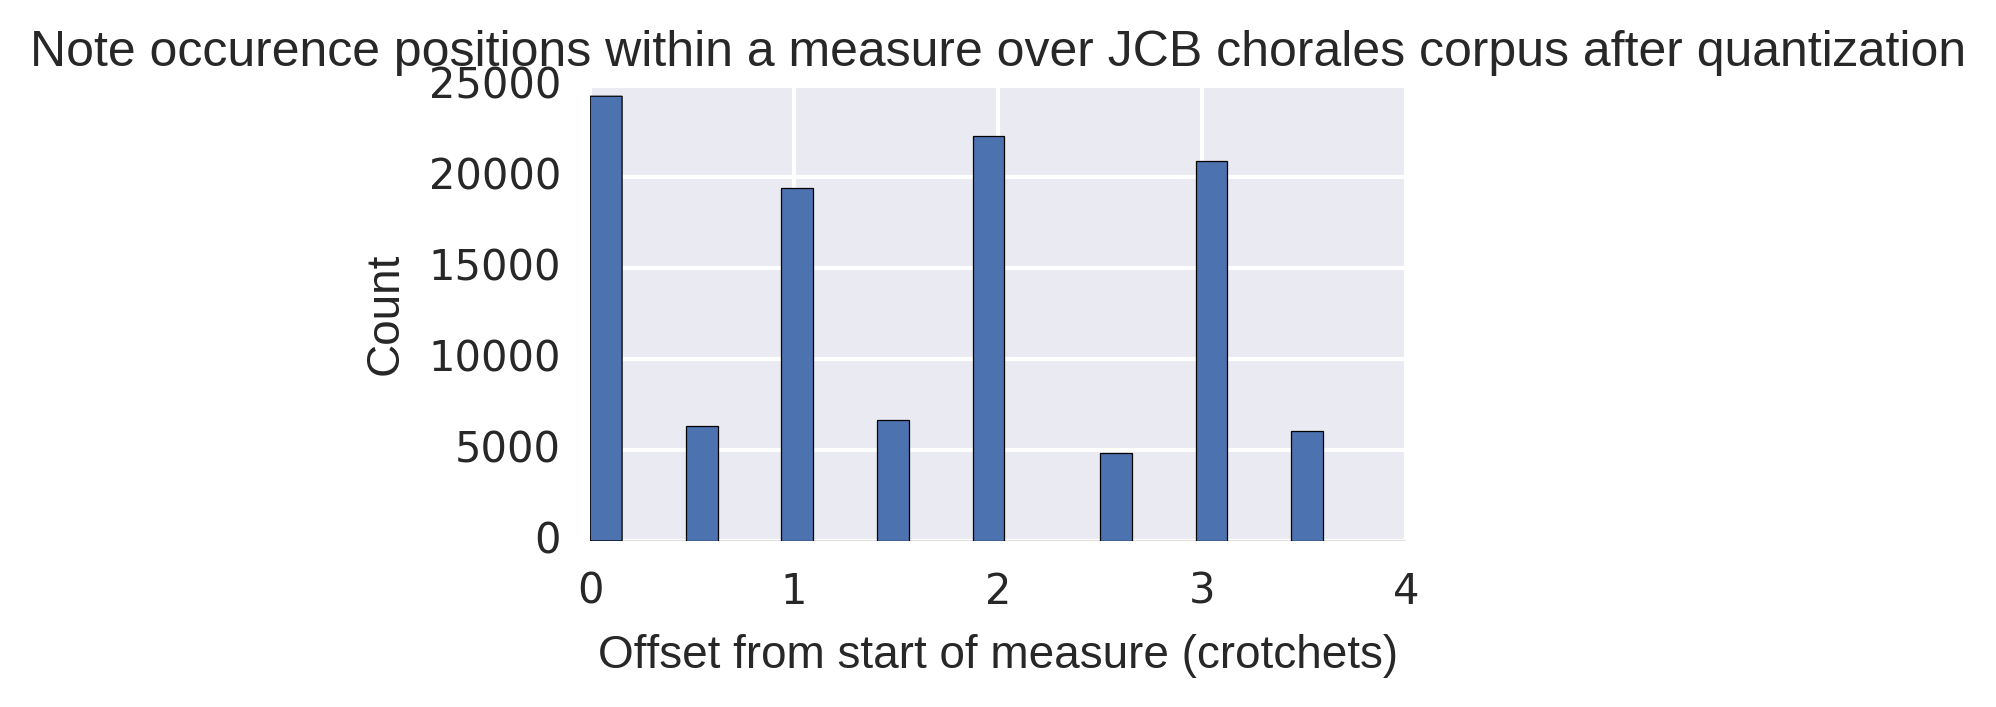
\includegraphics[width=1.0\linewidth]{meter-usage-quantized.png}
        %%% Creator: Matplotlib, PGF backend
%%
%% To include the figure in your LaTeX document, write
%%   \input{<filename>.pgf}
%%
%% Make sure the required packages are loaded in your preamble
%%   \usepackage{pgf}
%%
%% Figures using additional raster images can only be included by \input if
%% they are in the same directory as the main LaTeX file. For loading figures
%% from other directories you can use the `import` package
%%   \usepackage{import}
%% and then include the figures with
%%   \import{<path to file>}{<filename>.pgf}
%%
%% Matplotlib used the following preamble
%%   \usepackage[utf8x]{inputenc}
%%   \usepackage[T1]{fontenc}
%%   \usepackage{fontspec}
%%
\begingroup%
\makeatletter%
\begin{pgfpicture}%
\pgfpathrectangle{\pgfpointorigin}{\pgfqpoint{3.120454in}{1.784090in}}%
\pgfusepath{use as bounding box, clip}%
\begin{pgfscope}%
\pgfsetbuttcap%
\pgfsetmiterjoin%
\definecolor{currentfill}{rgb}{1.000000,1.000000,1.000000}%
\pgfsetfillcolor{currentfill}%
\pgfsetlinewidth{0.000000pt}%
\definecolor{currentstroke}{rgb}{1.000000,1.000000,1.000000}%
\pgfsetstrokecolor{currentstroke}%
\pgfsetdash{}{0pt}%
\pgfpathmoveto{\pgfqpoint{0.000000in}{0.000000in}}%
\pgfpathlineto{\pgfqpoint{3.120454in}{0.000000in}}%
\pgfpathlineto{\pgfqpoint{3.120454in}{1.784090in}}%
\pgfpathlineto{\pgfqpoint{0.000000in}{1.784090in}}%
\pgfpathclose%
\pgfusepath{fill}%
\end{pgfscope}%
\begin{pgfscope}%
\pgfsetbuttcap%
\pgfsetmiterjoin%
\definecolor{currentfill}{rgb}{0.917647,0.917647,0.949020}%
\pgfsetfillcolor{currentfill}%
\pgfsetlinewidth{0.000000pt}%
\definecolor{currentstroke}{rgb}{0.000000,0.000000,0.000000}%
\pgfsetstrokecolor{currentstroke}%
\pgfsetstrokeopacity{0.000000}%
\pgfsetdash{}{0pt}%
\pgfpathmoveto{\pgfqpoint{0.685143in}{0.504222in}}%
\pgfpathlineto{\pgfqpoint{2.711099in}{0.504222in}}%
\pgfpathlineto{\pgfqpoint{2.711099in}{1.489645in}}%
\pgfpathlineto{\pgfqpoint{0.685143in}{1.489645in}}%
\pgfpathclose%
\pgfusepath{fill}%
\end{pgfscope}%
\begin{pgfscope}%
\pgfpathrectangle{\pgfqpoint{0.685143in}{0.504222in}}{\pgfqpoint{2.025956in}{0.985424in}} %
\pgfusepath{clip}%
\pgfsetroundcap%
\pgfsetroundjoin%
\pgfsetlinewidth{1.003750pt}%
\definecolor{currentstroke}{rgb}{1.000000,1.000000,1.000000}%
\pgfsetstrokecolor{currentstroke}%
\pgfsetdash{}{0pt}%
\pgfpathmoveto{\pgfqpoint{0.685143in}{0.504222in}}%
\pgfpathlineto{\pgfqpoint{0.685143in}{1.489645in}}%
\pgfusepath{stroke}%
\end{pgfscope}%
\begin{pgfscope}%
\pgfsetbuttcap%
\pgfsetroundjoin%
\definecolor{currentfill}{rgb}{0.501961,0.501961,0.501961}%
\pgfsetfillcolor{currentfill}%
\pgfsetlinewidth{1.003750pt}%
\definecolor{currentstroke}{rgb}{0.501961,0.501961,0.501961}%
\pgfsetstrokecolor{currentstroke}%
\pgfsetdash{}{0pt}%
\pgfsys@defobject{currentmarker}{\pgfqpoint{0.000000in}{0.000000in}}{\pgfqpoint{0.000000in}{0.000000in}}{%
\pgfpathmoveto{\pgfqpoint{0.000000in}{0.000000in}}%
\pgfpathlineto{\pgfqpoint{0.000000in}{0.000000in}}%
\pgfusepath{stroke,fill}%
}%
\begin{pgfscope}%
\pgfsys@transformshift{0.685143in}{0.504222in}%
\pgfsys@useobject{currentmarker}{}%
\end{pgfscope}%
\end{pgfscope}%
\begin{pgfscope}%
\definecolor{textcolor}{rgb}{0.150000,0.150000,0.150000}%
\pgfsetstrokecolor{textcolor}%
\pgfsetfillcolor{textcolor}%
\pgftext[x=0.685143in,y=0.407000in,,top]{\color{textcolor}\rmfamily\fontsize{8.000000}{9.600000}\selectfont \(\displaystyle 0\)}%
\end{pgfscope}%
\begin{pgfscope}%
\pgfpathrectangle{\pgfqpoint{0.685143in}{0.504222in}}{\pgfqpoint{2.025956in}{0.985424in}} %
\pgfusepath{clip}%
\pgfsetroundcap%
\pgfsetroundjoin%
\pgfsetlinewidth{1.003750pt}%
\definecolor{currentstroke}{rgb}{1.000000,1.000000,1.000000}%
\pgfsetstrokecolor{currentstroke}%
\pgfsetdash{}{0pt}%
\pgfpathmoveto{\pgfqpoint{1.191632in}{0.504222in}}%
\pgfpathlineto{\pgfqpoint{1.191632in}{1.489645in}}%
\pgfusepath{stroke}%
\end{pgfscope}%
\begin{pgfscope}%
\pgfsetbuttcap%
\pgfsetroundjoin%
\definecolor{currentfill}{rgb}{0.501961,0.501961,0.501961}%
\pgfsetfillcolor{currentfill}%
\pgfsetlinewidth{1.003750pt}%
\definecolor{currentstroke}{rgb}{0.501961,0.501961,0.501961}%
\pgfsetstrokecolor{currentstroke}%
\pgfsetdash{}{0pt}%
\pgfsys@defobject{currentmarker}{\pgfqpoint{0.000000in}{0.000000in}}{\pgfqpoint{0.000000in}{0.000000in}}{%
\pgfpathmoveto{\pgfqpoint{0.000000in}{0.000000in}}%
\pgfpathlineto{\pgfqpoint{0.000000in}{0.000000in}}%
\pgfusepath{stroke,fill}%
}%
\begin{pgfscope}%
\pgfsys@transformshift{1.191632in}{0.504222in}%
\pgfsys@useobject{currentmarker}{}%
\end{pgfscope}%
\end{pgfscope}%
\begin{pgfscope}%
\definecolor{textcolor}{rgb}{0.150000,0.150000,0.150000}%
\pgfsetstrokecolor{textcolor}%
\pgfsetfillcolor{textcolor}%
\pgftext[x=1.191632in,y=0.407000in,,top]{\color{textcolor}\rmfamily\fontsize{8.000000}{9.600000}\selectfont \(\displaystyle 1\)}%
\end{pgfscope}%
\begin{pgfscope}%
\pgfpathrectangle{\pgfqpoint{0.685143in}{0.504222in}}{\pgfqpoint{2.025956in}{0.985424in}} %
\pgfusepath{clip}%
\pgfsetroundcap%
\pgfsetroundjoin%
\pgfsetlinewidth{1.003750pt}%
\definecolor{currentstroke}{rgb}{1.000000,1.000000,1.000000}%
\pgfsetstrokecolor{currentstroke}%
\pgfsetdash{}{0pt}%
\pgfpathmoveto{\pgfqpoint{1.698121in}{0.504222in}}%
\pgfpathlineto{\pgfqpoint{1.698121in}{1.489645in}}%
\pgfusepath{stroke}%
\end{pgfscope}%
\begin{pgfscope}%
\pgfsetbuttcap%
\pgfsetroundjoin%
\definecolor{currentfill}{rgb}{0.501961,0.501961,0.501961}%
\pgfsetfillcolor{currentfill}%
\pgfsetlinewidth{1.003750pt}%
\definecolor{currentstroke}{rgb}{0.501961,0.501961,0.501961}%
\pgfsetstrokecolor{currentstroke}%
\pgfsetdash{}{0pt}%
\pgfsys@defobject{currentmarker}{\pgfqpoint{0.000000in}{0.000000in}}{\pgfqpoint{0.000000in}{0.000000in}}{%
\pgfpathmoveto{\pgfqpoint{0.000000in}{0.000000in}}%
\pgfpathlineto{\pgfqpoint{0.000000in}{0.000000in}}%
\pgfusepath{stroke,fill}%
}%
\begin{pgfscope}%
\pgfsys@transformshift{1.698121in}{0.504222in}%
\pgfsys@useobject{currentmarker}{}%
\end{pgfscope}%
\end{pgfscope}%
\begin{pgfscope}%
\definecolor{textcolor}{rgb}{0.150000,0.150000,0.150000}%
\pgfsetstrokecolor{textcolor}%
\pgfsetfillcolor{textcolor}%
\pgftext[x=1.698121in,y=0.407000in,,top]{\color{textcolor}\rmfamily\fontsize{8.000000}{9.600000}\selectfont \(\displaystyle 2\)}%
\end{pgfscope}%
\begin{pgfscope}%
\pgfpathrectangle{\pgfqpoint{0.685143in}{0.504222in}}{\pgfqpoint{2.025956in}{0.985424in}} %
\pgfusepath{clip}%
\pgfsetroundcap%
\pgfsetroundjoin%
\pgfsetlinewidth{1.003750pt}%
\definecolor{currentstroke}{rgb}{1.000000,1.000000,1.000000}%
\pgfsetstrokecolor{currentstroke}%
\pgfsetdash{}{0pt}%
\pgfpathmoveto{\pgfqpoint{2.204610in}{0.504222in}}%
\pgfpathlineto{\pgfqpoint{2.204610in}{1.489645in}}%
\pgfusepath{stroke}%
\end{pgfscope}%
\begin{pgfscope}%
\pgfsetbuttcap%
\pgfsetroundjoin%
\definecolor{currentfill}{rgb}{0.501961,0.501961,0.501961}%
\pgfsetfillcolor{currentfill}%
\pgfsetlinewidth{1.003750pt}%
\definecolor{currentstroke}{rgb}{0.501961,0.501961,0.501961}%
\pgfsetstrokecolor{currentstroke}%
\pgfsetdash{}{0pt}%
\pgfsys@defobject{currentmarker}{\pgfqpoint{0.000000in}{0.000000in}}{\pgfqpoint{0.000000in}{0.000000in}}{%
\pgfpathmoveto{\pgfqpoint{0.000000in}{0.000000in}}%
\pgfpathlineto{\pgfqpoint{0.000000in}{0.000000in}}%
\pgfusepath{stroke,fill}%
}%
\begin{pgfscope}%
\pgfsys@transformshift{2.204610in}{0.504222in}%
\pgfsys@useobject{currentmarker}{}%
\end{pgfscope}%
\end{pgfscope}%
\begin{pgfscope}%
\definecolor{textcolor}{rgb}{0.150000,0.150000,0.150000}%
\pgfsetstrokecolor{textcolor}%
\pgfsetfillcolor{textcolor}%
\pgftext[x=2.204610in,y=0.407000in,,top]{\color{textcolor}\rmfamily\fontsize{8.000000}{9.600000}\selectfont \(\displaystyle 3\)}%
\end{pgfscope}%
\begin{pgfscope}%
\pgfpathrectangle{\pgfqpoint{0.685143in}{0.504222in}}{\pgfqpoint{2.025956in}{0.985424in}} %
\pgfusepath{clip}%
\pgfsetroundcap%
\pgfsetroundjoin%
\pgfsetlinewidth{1.003750pt}%
\definecolor{currentstroke}{rgb}{1.000000,1.000000,1.000000}%
\pgfsetstrokecolor{currentstroke}%
\pgfsetdash{}{0pt}%
\pgfpathmoveto{\pgfqpoint{2.711099in}{0.504222in}}%
\pgfpathlineto{\pgfqpoint{2.711099in}{1.489645in}}%
\pgfusepath{stroke}%
\end{pgfscope}%
\begin{pgfscope}%
\pgfsetbuttcap%
\pgfsetroundjoin%
\definecolor{currentfill}{rgb}{0.501961,0.501961,0.501961}%
\pgfsetfillcolor{currentfill}%
\pgfsetlinewidth{1.003750pt}%
\definecolor{currentstroke}{rgb}{0.501961,0.501961,0.501961}%
\pgfsetstrokecolor{currentstroke}%
\pgfsetdash{}{0pt}%
\pgfsys@defobject{currentmarker}{\pgfqpoint{0.000000in}{0.000000in}}{\pgfqpoint{0.000000in}{0.000000in}}{%
\pgfpathmoveto{\pgfqpoint{0.000000in}{0.000000in}}%
\pgfpathlineto{\pgfqpoint{0.000000in}{0.000000in}}%
\pgfusepath{stroke,fill}%
}%
\begin{pgfscope}%
\pgfsys@transformshift{2.711099in}{0.504222in}%
\pgfsys@useobject{currentmarker}{}%
\end{pgfscope}%
\end{pgfscope}%
\begin{pgfscope}%
\definecolor{textcolor}{rgb}{0.150000,0.150000,0.150000}%
\pgfsetstrokecolor{textcolor}%
\pgfsetfillcolor{textcolor}%
\pgftext[x=2.711099in,y=0.407000in,,top]{\color{textcolor}\rmfamily\fontsize{8.000000}{9.600000}\selectfont \(\displaystyle 4\)}%
\end{pgfscope}%
\begin{pgfscope}%
\definecolor{textcolor}{rgb}{0.150000,0.150000,0.150000}%
\pgfsetstrokecolor{textcolor}%
\pgfsetfillcolor{textcolor}%
\pgftext[x=1.698121in,y=0.238889in,,top]{\color{textcolor}\rmfamily\fontsize{10.000000}{12.000000}\selectfont Offset from start of measure (crotchets)}%
\end{pgfscope}%
\begin{pgfscope}%
\pgfpathrectangle{\pgfqpoint{0.685143in}{0.504222in}}{\pgfqpoint{2.025956in}{0.985424in}} %
\pgfusepath{clip}%
\pgfsetroundcap%
\pgfsetroundjoin%
\pgfsetlinewidth{1.003750pt}%
\definecolor{currentstroke}{rgb}{1.000000,1.000000,1.000000}%
\pgfsetstrokecolor{currentstroke}%
\pgfsetdash{}{0pt}%
\pgfpathmoveto{\pgfqpoint{0.685143in}{0.504222in}}%
\pgfpathlineto{\pgfqpoint{2.711099in}{0.504222in}}%
\pgfusepath{stroke}%
\end{pgfscope}%
\begin{pgfscope}%
\pgfsetbuttcap%
\pgfsetroundjoin%
\definecolor{currentfill}{rgb}{0.501961,0.501961,0.501961}%
\pgfsetfillcolor{currentfill}%
\pgfsetlinewidth{1.003750pt}%
\definecolor{currentstroke}{rgb}{0.501961,0.501961,0.501961}%
\pgfsetstrokecolor{currentstroke}%
\pgfsetdash{}{0pt}%
\pgfsys@defobject{currentmarker}{\pgfqpoint{0.000000in}{0.000000in}}{\pgfqpoint{0.000000in}{0.000000in}}{%
\pgfpathmoveto{\pgfqpoint{0.000000in}{0.000000in}}%
\pgfpathlineto{\pgfqpoint{0.000000in}{0.000000in}}%
\pgfusepath{stroke,fill}%
}%
\begin{pgfscope}%
\pgfsys@transformshift{0.685143in}{0.504222in}%
\pgfsys@useobject{currentmarker}{}%
\end{pgfscope}%
\end{pgfscope}%
\begin{pgfscope}%
\definecolor{textcolor}{rgb}{0.150000,0.150000,0.150000}%
\pgfsetstrokecolor{textcolor}%
\pgfsetfillcolor{textcolor}%
\pgftext[x=0.587921in,y=0.504222in,right,]{\color{textcolor}\rmfamily\fontsize{8.000000}{9.600000}\selectfont \(\displaystyle 0\)}%
\end{pgfscope}%
\begin{pgfscope}%
\pgfpathrectangle{\pgfqpoint{0.685143in}{0.504222in}}{\pgfqpoint{2.025956in}{0.985424in}} %
\pgfusepath{clip}%
\pgfsetroundcap%
\pgfsetroundjoin%
\pgfsetlinewidth{1.003750pt}%
\definecolor{currentstroke}{rgb}{1.000000,1.000000,1.000000}%
\pgfsetstrokecolor{currentstroke}%
\pgfsetdash{}{0pt}%
\pgfpathmoveto{\pgfqpoint{0.685143in}{0.701307in}}%
\pgfpathlineto{\pgfqpoint{2.711099in}{0.701307in}}%
\pgfusepath{stroke}%
\end{pgfscope}%
\begin{pgfscope}%
\pgfsetbuttcap%
\pgfsetroundjoin%
\definecolor{currentfill}{rgb}{0.501961,0.501961,0.501961}%
\pgfsetfillcolor{currentfill}%
\pgfsetlinewidth{1.003750pt}%
\definecolor{currentstroke}{rgb}{0.501961,0.501961,0.501961}%
\pgfsetstrokecolor{currentstroke}%
\pgfsetdash{}{0pt}%
\pgfsys@defobject{currentmarker}{\pgfqpoint{0.000000in}{0.000000in}}{\pgfqpoint{0.000000in}{0.000000in}}{%
\pgfpathmoveto{\pgfqpoint{0.000000in}{0.000000in}}%
\pgfpathlineto{\pgfqpoint{0.000000in}{0.000000in}}%
\pgfusepath{stroke,fill}%
}%
\begin{pgfscope}%
\pgfsys@transformshift{0.685143in}{0.701307in}%
\pgfsys@useobject{currentmarker}{}%
\end{pgfscope}%
\end{pgfscope}%
\begin{pgfscope}%
\definecolor{textcolor}{rgb}{0.150000,0.150000,0.150000}%
\pgfsetstrokecolor{textcolor}%
\pgfsetfillcolor{textcolor}%
\pgftext[x=0.587921in,y=0.701307in,right,]{\color{textcolor}\rmfamily\fontsize{8.000000}{9.600000}\selectfont \(\displaystyle 5000\)}%
\end{pgfscope}%
\begin{pgfscope}%
\pgfpathrectangle{\pgfqpoint{0.685143in}{0.504222in}}{\pgfqpoint{2.025956in}{0.985424in}} %
\pgfusepath{clip}%
\pgfsetroundcap%
\pgfsetroundjoin%
\pgfsetlinewidth{1.003750pt}%
\definecolor{currentstroke}{rgb}{1.000000,1.000000,1.000000}%
\pgfsetstrokecolor{currentstroke}%
\pgfsetdash{}{0pt}%
\pgfpathmoveto{\pgfqpoint{0.685143in}{0.898391in}}%
\pgfpathlineto{\pgfqpoint{2.711099in}{0.898391in}}%
\pgfusepath{stroke}%
\end{pgfscope}%
\begin{pgfscope}%
\pgfsetbuttcap%
\pgfsetroundjoin%
\definecolor{currentfill}{rgb}{0.501961,0.501961,0.501961}%
\pgfsetfillcolor{currentfill}%
\pgfsetlinewidth{1.003750pt}%
\definecolor{currentstroke}{rgb}{0.501961,0.501961,0.501961}%
\pgfsetstrokecolor{currentstroke}%
\pgfsetdash{}{0pt}%
\pgfsys@defobject{currentmarker}{\pgfqpoint{0.000000in}{0.000000in}}{\pgfqpoint{0.000000in}{0.000000in}}{%
\pgfpathmoveto{\pgfqpoint{0.000000in}{0.000000in}}%
\pgfpathlineto{\pgfqpoint{0.000000in}{0.000000in}}%
\pgfusepath{stroke,fill}%
}%
\begin{pgfscope}%
\pgfsys@transformshift{0.685143in}{0.898391in}%
\pgfsys@useobject{currentmarker}{}%
\end{pgfscope}%
\end{pgfscope}%
\begin{pgfscope}%
\definecolor{textcolor}{rgb}{0.150000,0.150000,0.150000}%
\pgfsetstrokecolor{textcolor}%
\pgfsetfillcolor{textcolor}%
\pgftext[x=0.587921in,y=0.898391in,right,]{\color{textcolor}\rmfamily\fontsize{8.000000}{9.600000}\selectfont \(\displaystyle 10000\)}%
\end{pgfscope}%
\begin{pgfscope}%
\pgfpathrectangle{\pgfqpoint{0.685143in}{0.504222in}}{\pgfqpoint{2.025956in}{0.985424in}} %
\pgfusepath{clip}%
\pgfsetroundcap%
\pgfsetroundjoin%
\pgfsetlinewidth{1.003750pt}%
\definecolor{currentstroke}{rgb}{1.000000,1.000000,1.000000}%
\pgfsetstrokecolor{currentstroke}%
\pgfsetdash{}{0pt}%
\pgfpathmoveto{\pgfqpoint{0.685143in}{1.095476in}}%
\pgfpathlineto{\pgfqpoint{2.711099in}{1.095476in}}%
\pgfusepath{stroke}%
\end{pgfscope}%
\begin{pgfscope}%
\pgfsetbuttcap%
\pgfsetroundjoin%
\definecolor{currentfill}{rgb}{0.501961,0.501961,0.501961}%
\pgfsetfillcolor{currentfill}%
\pgfsetlinewidth{1.003750pt}%
\definecolor{currentstroke}{rgb}{0.501961,0.501961,0.501961}%
\pgfsetstrokecolor{currentstroke}%
\pgfsetdash{}{0pt}%
\pgfsys@defobject{currentmarker}{\pgfqpoint{0.000000in}{0.000000in}}{\pgfqpoint{0.000000in}{0.000000in}}{%
\pgfpathmoveto{\pgfqpoint{0.000000in}{0.000000in}}%
\pgfpathlineto{\pgfqpoint{0.000000in}{0.000000in}}%
\pgfusepath{stroke,fill}%
}%
\begin{pgfscope}%
\pgfsys@transformshift{0.685143in}{1.095476in}%
\pgfsys@useobject{currentmarker}{}%
\end{pgfscope}%
\end{pgfscope}%
\begin{pgfscope}%
\definecolor{textcolor}{rgb}{0.150000,0.150000,0.150000}%
\pgfsetstrokecolor{textcolor}%
\pgfsetfillcolor{textcolor}%
\pgftext[x=0.587921in,y=1.095476in,right,]{\color{textcolor}\rmfamily\fontsize{8.000000}{9.600000}\selectfont \(\displaystyle 15000\)}%
\end{pgfscope}%
\begin{pgfscope}%
\pgfpathrectangle{\pgfqpoint{0.685143in}{0.504222in}}{\pgfqpoint{2.025956in}{0.985424in}} %
\pgfusepath{clip}%
\pgfsetroundcap%
\pgfsetroundjoin%
\pgfsetlinewidth{1.003750pt}%
\definecolor{currentstroke}{rgb}{1.000000,1.000000,1.000000}%
\pgfsetstrokecolor{currentstroke}%
\pgfsetdash{}{0pt}%
\pgfpathmoveto{\pgfqpoint{0.685143in}{1.292561in}}%
\pgfpathlineto{\pgfqpoint{2.711099in}{1.292561in}}%
\pgfusepath{stroke}%
\end{pgfscope}%
\begin{pgfscope}%
\pgfsetbuttcap%
\pgfsetroundjoin%
\definecolor{currentfill}{rgb}{0.501961,0.501961,0.501961}%
\pgfsetfillcolor{currentfill}%
\pgfsetlinewidth{1.003750pt}%
\definecolor{currentstroke}{rgb}{0.501961,0.501961,0.501961}%
\pgfsetstrokecolor{currentstroke}%
\pgfsetdash{}{0pt}%
\pgfsys@defobject{currentmarker}{\pgfqpoint{0.000000in}{0.000000in}}{\pgfqpoint{0.000000in}{0.000000in}}{%
\pgfpathmoveto{\pgfqpoint{0.000000in}{0.000000in}}%
\pgfpathlineto{\pgfqpoint{0.000000in}{0.000000in}}%
\pgfusepath{stroke,fill}%
}%
\begin{pgfscope}%
\pgfsys@transformshift{0.685143in}{1.292561in}%
\pgfsys@useobject{currentmarker}{}%
\end{pgfscope}%
\end{pgfscope}%
\begin{pgfscope}%
\definecolor{textcolor}{rgb}{0.150000,0.150000,0.150000}%
\pgfsetstrokecolor{textcolor}%
\pgfsetfillcolor{textcolor}%
\pgftext[x=0.587921in,y=1.292561in,right,]{\color{textcolor}\rmfamily\fontsize{8.000000}{9.600000}\selectfont \(\displaystyle 20000\)}%
\end{pgfscope}%
\begin{pgfscope}%
\pgfpathrectangle{\pgfqpoint{0.685143in}{0.504222in}}{\pgfqpoint{2.025956in}{0.985424in}} %
\pgfusepath{clip}%
\pgfsetroundcap%
\pgfsetroundjoin%
\pgfsetlinewidth{1.003750pt}%
\definecolor{currentstroke}{rgb}{1.000000,1.000000,1.000000}%
\pgfsetstrokecolor{currentstroke}%
\pgfsetdash{}{0pt}%
\pgfpathmoveto{\pgfqpoint{0.685143in}{1.489645in}}%
\pgfpathlineto{\pgfqpoint{2.711099in}{1.489645in}}%
\pgfusepath{stroke}%
\end{pgfscope}%
\begin{pgfscope}%
\pgfsetbuttcap%
\pgfsetroundjoin%
\definecolor{currentfill}{rgb}{0.501961,0.501961,0.501961}%
\pgfsetfillcolor{currentfill}%
\pgfsetlinewidth{1.003750pt}%
\definecolor{currentstroke}{rgb}{0.501961,0.501961,0.501961}%
\pgfsetstrokecolor{currentstroke}%
\pgfsetdash{}{0pt}%
\pgfsys@defobject{currentmarker}{\pgfqpoint{0.000000in}{0.000000in}}{\pgfqpoint{0.000000in}{0.000000in}}{%
\pgfpathmoveto{\pgfqpoint{0.000000in}{0.000000in}}%
\pgfpathlineto{\pgfqpoint{0.000000in}{0.000000in}}%
\pgfusepath{stroke,fill}%
}%
\begin{pgfscope}%
\pgfsys@transformshift{0.685143in}{1.489645in}%
\pgfsys@useobject{currentmarker}{}%
\end{pgfscope}%
\end{pgfscope}%
\begin{pgfscope}%
\definecolor{textcolor}{rgb}{0.150000,0.150000,0.150000}%
\pgfsetstrokecolor{textcolor}%
\pgfsetfillcolor{textcolor}%
\pgftext[x=0.587921in,y=1.489645in,right,]{\color{textcolor}\rmfamily\fontsize{8.000000}{9.600000}\selectfont \(\displaystyle 25000\)}%
\end{pgfscope}%
\begin{pgfscope}%
\definecolor{textcolor}{rgb}{0.150000,0.150000,0.150000}%
\pgfsetstrokecolor{textcolor}%
\pgfsetfillcolor{textcolor}%
\pgftext[x=0.223333in,y=0.996934in,,bottom,rotate=90.000000]{\color{textcolor}\rmfamily\fontsize{10.000000}{12.000000}\selectfont Count}%
\end{pgfscope}%
\begin{pgfscope}%
\pgfpathrectangle{\pgfqpoint{0.685143in}{0.504222in}}{\pgfqpoint{2.025956in}{0.985424in}} %
\pgfusepath{clip}%
\pgfsetbuttcap%
\pgfsetmiterjoin%
\definecolor{currentfill}{rgb}{0.298039,0.447059,0.690196}%
\pgfsetfillcolor{currentfill}%
\pgfsetlinewidth{0.301125pt}%
\definecolor{currentstroke}{rgb}{0.000000,0.000000,0.000000}%
\pgfsetstrokecolor{currentstroke}%
\pgfsetdash{}{0pt}%
\pgfpathmoveto{\pgfqpoint{0.685143in}{0.504222in}}%
\pgfpathlineto{\pgfqpoint{0.764282in}{0.504222in}}%
\pgfpathlineto{\pgfqpoint{0.764282in}{1.379712in}}%
\pgfpathlineto{\pgfqpoint{0.685143in}{1.379712in}}%
\pgfpathclose%
\pgfusepath{stroke,fill}%
\end{pgfscope}%
\begin{pgfscope}%
\pgfpathrectangle{\pgfqpoint{0.685143in}{0.504222in}}{\pgfqpoint{2.025956in}{0.985424in}} %
\pgfusepath{clip}%
\pgfsetbuttcap%
\pgfsetmiterjoin%
\definecolor{currentfill}{rgb}{0.298039,0.447059,0.690196}%
\pgfsetfillcolor{currentfill}%
\pgfsetlinewidth{0.301125pt}%
\definecolor{currentstroke}{rgb}{0.000000,0.000000,0.000000}%
\pgfsetstrokecolor{currentstroke}%
\pgfsetdash{}{0pt}%
\pgfpathmoveto{\pgfqpoint{0.764282in}{0.504222in}}%
\pgfpathlineto{\pgfqpoint{0.843421in}{0.504222in}}%
\pgfpathlineto{\pgfqpoint{0.843421in}{0.504222in}}%
\pgfpathlineto{\pgfqpoint{0.764282in}{0.504222in}}%
\pgfpathclose%
\pgfusepath{stroke,fill}%
\end{pgfscope}%
\begin{pgfscope}%
\pgfpathrectangle{\pgfqpoint{0.685143in}{0.504222in}}{\pgfqpoint{2.025956in}{0.985424in}} %
\pgfusepath{clip}%
\pgfsetbuttcap%
\pgfsetmiterjoin%
\definecolor{currentfill}{rgb}{0.298039,0.447059,0.690196}%
\pgfsetfillcolor{currentfill}%
\pgfsetlinewidth{0.301125pt}%
\definecolor{currentstroke}{rgb}{0.000000,0.000000,0.000000}%
\pgfsetstrokecolor{currentstroke}%
\pgfsetdash{}{0pt}%
\pgfpathmoveto{\pgfqpoint{0.843421in}{0.504222in}}%
\pgfpathlineto{\pgfqpoint{0.922560in}{0.504222in}}%
\pgfpathlineto{\pgfqpoint{0.922560in}{0.504222in}}%
\pgfpathlineto{\pgfqpoint{0.843421in}{0.504222in}}%
\pgfpathclose%
\pgfusepath{stroke,fill}%
\end{pgfscope}%
\begin{pgfscope}%
\pgfpathrectangle{\pgfqpoint{0.685143in}{0.504222in}}{\pgfqpoint{2.025956in}{0.985424in}} %
\pgfusepath{clip}%
\pgfsetbuttcap%
\pgfsetmiterjoin%
\definecolor{currentfill}{rgb}{0.298039,0.447059,0.690196}%
\pgfsetfillcolor{currentfill}%
\pgfsetlinewidth{0.301125pt}%
\definecolor{currentstroke}{rgb}{0.000000,0.000000,0.000000}%
\pgfsetstrokecolor{currentstroke}%
\pgfsetdash{}{0pt}%
\pgfpathmoveto{\pgfqpoint{0.922560in}{0.504222in}}%
\pgfpathlineto{\pgfqpoint{1.001699in}{0.504222in}}%
\pgfpathlineto{\pgfqpoint{1.001699in}{0.712186in}}%
\pgfpathlineto{\pgfqpoint{0.922560in}{0.712186in}}%
\pgfpathclose%
\pgfusepath{stroke,fill}%
\end{pgfscope}%
\begin{pgfscope}%
\pgfpathrectangle{\pgfqpoint{0.685143in}{0.504222in}}{\pgfqpoint{2.025956in}{0.985424in}} %
\pgfusepath{clip}%
\pgfsetbuttcap%
\pgfsetmiterjoin%
\definecolor{currentfill}{rgb}{0.298039,0.447059,0.690196}%
\pgfsetfillcolor{currentfill}%
\pgfsetlinewidth{0.301125pt}%
\definecolor{currentstroke}{rgb}{0.000000,0.000000,0.000000}%
\pgfsetstrokecolor{currentstroke}%
\pgfsetdash{}{0pt}%
\pgfpathmoveto{\pgfqpoint{1.001699in}{0.504222in}}%
\pgfpathlineto{\pgfqpoint{1.080837in}{0.504222in}}%
\pgfpathlineto{\pgfqpoint{1.080837in}{0.504222in}}%
\pgfpathlineto{\pgfqpoint{1.001699in}{0.504222in}}%
\pgfpathclose%
\pgfusepath{stroke,fill}%
\end{pgfscope}%
\begin{pgfscope}%
\pgfpathrectangle{\pgfqpoint{0.685143in}{0.504222in}}{\pgfqpoint{2.025956in}{0.985424in}} %
\pgfusepath{clip}%
\pgfsetbuttcap%
\pgfsetmiterjoin%
\definecolor{currentfill}{rgb}{0.298039,0.447059,0.690196}%
\pgfsetfillcolor{currentfill}%
\pgfsetlinewidth{0.301125pt}%
\definecolor{currentstroke}{rgb}{0.000000,0.000000,0.000000}%
\pgfsetstrokecolor{currentstroke}%
\pgfsetdash{}{0pt}%
\pgfpathmoveto{\pgfqpoint{1.080837in}{0.504222in}}%
\pgfpathlineto{\pgfqpoint{1.159976in}{0.504222in}}%
\pgfpathlineto{\pgfqpoint{1.159976in}{0.504222in}}%
\pgfpathlineto{\pgfqpoint{1.080837in}{0.504222in}}%
\pgfpathclose%
\pgfusepath{stroke,fill}%
\end{pgfscope}%
\begin{pgfscope}%
\pgfpathrectangle{\pgfqpoint{0.685143in}{0.504222in}}{\pgfqpoint{2.025956in}{0.985424in}} %
\pgfusepath{clip}%
\pgfsetbuttcap%
\pgfsetmiterjoin%
\definecolor{currentfill}{rgb}{0.298039,0.447059,0.690196}%
\pgfsetfillcolor{currentfill}%
\pgfsetlinewidth{0.301125pt}%
\definecolor{currentstroke}{rgb}{0.000000,0.000000,0.000000}%
\pgfsetstrokecolor{currentstroke}%
\pgfsetdash{}{0pt}%
\pgfpathmoveto{\pgfqpoint{1.159976in}{0.504222in}}%
\pgfpathlineto{\pgfqpoint{1.239115in}{0.504222in}}%
\pgfpathlineto{\pgfqpoint{1.239115in}{1.199379in}}%
\pgfpathlineto{\pgfqpoint{1.159976in}{1.199379in}}%
\pgfpathclose%
\pgfusepath{stroke,fill}%
\end{pgfscope}%
\begin{pgfscope}%
\pgfpathrectangle{\pgfqpoint{0.685143in}{0.504222in}}{\pgfqpoint{2.025956in}{0.985424in}} %
\pgfusepath{clip}%
\pgfsetbuttcap%
\pgfsetmiterjoin%
\definecolor{currentfill}{rgb}{0.298039,0.447059,0.690196}%
\pgfsetfillcolor{currentfill}%
\pgfsetlinewidth{0.301125pt}%
\definecolor{currentstroke}{rgb}{0.000000,0.000000,0.000000}%
\pgfsetstrokecolor{currentstroke}%
\pgfsetdash{}{0pt}%
\pgfpathmoveto{\pgfqpoint{1.239115in}{0.504222in}}%
\pgfpathlineto{\pgfqpoint{1.318254in}{0.504222in}}%
\pgfpathlineto{\pgfqpoint{1.318254in}{0.504222in}}%
\pgfpathlineto{\pgfqpoint{1.239115in}{0.504222in}}%
\pgfpathclose%
\pgfusepath{stroke,fill}%
\end{pgfscope}%
\begin{pgfscope}%
\pgfpathrectangle{\pgfqpoint{0.685143in}{0.504222in}}{\pgfqpoint{2.025956in}{0.985424in}} %
\pgfusepath{clip}%
\pgfsetbuttcap%
\pgfsetmiterjoin%
\definecolor{currentfill}{rgb}{0.298039,0.447059,0.690196}%
\pgfsetfillcolor{currentfill}%
\pgfsetlinewidth{0.301125pt}%
\definecolor{currentstroke}{rgb}{0.000000,0.000000,0.000000}%
\pgfsetstrokecolor{currentstroke}%
\pgfsetdash{}{0pt}%
\pgfpathmoveto{\pgfqpoint{1.318254in}{0.504222in}}%
\pgfpathlineto{\pgfqpoint{1.397393in}{0.504222in}}%
\pgfpathlineto{\pgfqpoint{1.397393in}{0.504222in}}%
\pgfpathlineto{\pgfqpoint{1.318254in}{0.504222in}}%
\pgfpathclose%
\pgfusepath{stroke,fill}%
\end{pgfscope}%
\begin{pgfscope}%
\pgfpathrectangle{\pgfqpoint{0.685143in}{0.504222in}}{\pgfqpoint{2.025956in}{0.985424in}} %
\pgfusepath{clip}%
\pgfsetbuttcap%
\pgfsetmiterjoin%
\definecolor{currentfill}{rgb}{0.298039,0.447059,0.690196}%
\pgfsetfillcolor{currentfill}%
\pgfsetlinewidth{0.301125pt}%
\definecolor{currentstroke}{rgb}{0.000000,0.000000,0.000000}%
\pgfsetstrokecolor{currentstroke}%
\pgfsetdash{}{0pt}%
\pgfpathmoveto{\pgfqpoint{1.397393in}{0.504222in}}%
\pgfpathlineto{\pgfqpoint{1.476532in}{0.504222in}}%
\pgfpathlineto{\pgfqpoint{1.476532in}{0.720227in}}%
\pgfpathlineto{\pgfqpoint{1.397393in}{0.720227in}}%
\pgfpathclose%
\pgfusepath{stroke,fill}%
\end{pgfscope}%
\begin{pgfscope}%
\pgfpathrectangle{\pgfqpoint{0.685143in}{0.504222in}}{\pgfqpoint{2.025956in}{0.985424in}} %
\pgfusepath{clip}%
\pgfsetbuttcap%
\pgfsetmiterjoin%
\definecolor{currentfill}{rgb}{0.298039,0.447059,0.690196}%
\pgfsetfillcolor{currentfill}%
\pgfsetlinewidth{0.301125pt}%
\definecolor{currentstroke}{rgb}{0.000000,0.000000,0.000000}%
\pgfsetstrokecolor{currentstroke}%
\pgfsetdash{}{0pt}%
\pgfpathmoveto{\pgfqpoint{1.476532in}{0.504222in}}%
\pgfpathlineto{\pgfqpoint{1.555671in}{0.504222in}}%
\pgfpathlineto{\pgfqpoint{1.555671in}{0.504222in}}%
\pgfpathlineto{\pgfqpoint{1.476532in}{0.504222in}}%
\pgfpathclose%
\pgfusepath{stroke,fill}%
\end{pgfscope}%
\begin{pgfscope}%
\pgfpathrectangle{\pgfqpoint{0.685143in}{0.504222in}}{\pgfqpoint{2.025956in}{0.985424in}} %
\pgfusepath{clip}%
\pgfsetbuttcap%
\pgfsetmiterjoin%
\definecolor{currentfill}{rgb}{0.298039,0.447059,0.690196}%
\pgfsetfillcolor{currentfill}%
\pgfsetlinewidth{0.301125pt}%
\definecolor{currentstroke}{rgb}{0.000000,0.000000,0.000000}%
\pgfsetstrokecolor{currentstroke}%
\pgfsetdash{}{0pt}%
\pgfpathmoveto{\pgfqpoint{1.555671in}{0.504222in}}%
\pgfpathlineto{\pgfqpoint{1.634810in}{0.504222in}}%
\pgfpathlineto{\pgfqpoint{1.634810in}{0.504222in}}%
\pgfpathlineto{\pgfqpoint{1.555671in}{0.504222in}}%
\pgfpathclose%
\pgfusepath{stroke,fill}%
\end{pgfscope}%
\begin{pgfscope}%
\pgfpathrectangle{\pgfqpoint{0.685143in}{0.504222in}}{\pgfqpoint{2.025956in}{0.985424in}} %
\pgfusepath{clip}%
\pgfsetbuttcap%
\pgfsetmiterjoin%
\definecolor{currentfill}{rgb}{0.298039,0.447059,0.690196}%
\pgfsetfillcolor{currentfill}%
\pgfsetlinewidth{0.301125pt}%
\definecolor{currentstroke}{rgb}{0.000000,0.000000,0.000000}%
\pgfsetstrokecolor{currentstroke}%
\pgfsetdash{}{0pt}%
\pgfpathmoveto{\pgfqpoint{1.634810in}{0.504222in}}%
\pgfpathlineto{\pgfqpoint{1.713949in}{0.504222in}}%
\pgfpathlineto{\pgfqpoint{1.713949in}{1.300168in}}%
\pgfpathlineto{\pgfqpoint{1.634810in}{1.300168in}}%
\pgfpathclose%
\pgfusepath{stroke,fill}%
\end{pgfscope}%
\begin{pgfscope}%
\pgfpathrectangle{\pgfqpoint{0.685143in}{0.504222in}}{\pgfqpoint{2.025956in}{0.985424in}} %
\pgfusepath{clip}%
\pgfsetbuttcap%
\pgfsetmiterjoin%
\definecolor{currentfill}{rgb}{0.298039,0.447059,0.690196}%
\pgfsetfillcolor{currentfill}%
\pgfsetlinewidth{0.301125pt}%
\definecolor{currentstroke}{rgb}{0.000000,0.000000,0.000000}%
\pgfsetstrokecolor{currentstroke}%
\pgfsetdash{}{0pt}%
\pgfpathmoveto{\pgfqpoint{1.713949in}{0.504222in}}%
\pgfpathlineto{\pgfqpoint{1.793088in}{0.504222in}}%
\pgfpathlineto{\pgfqpoint{1.793088in}{0.504222in}}%
\pgfpathlineto{\pgfqpoint{1.713949in}{0.504222in}}%
\pgfpathclose%
\pgfusepath{stroke,fill}%
\end{pgfscope}%
\begin{pgfscope}%
\pgfpathrectangle{\pgfqpoint{0.685143in}{0.504222in}}{\pgfqpoint{2.025956in}{0.985424in}} %
\pgfusepath{clip}%
\pgfsetbuttcap%
\pgfsetmiterjoin%
\definecolor{currentfill}{rgb}{0.298039,0.447059,0.690196}%
\pgfsetfillcolor{currentfill}%
\pgfsetlinewidth{0.301125pt}%
\definecolor{currentstroke}{rgb}{0.000000,0.000000,0.000000}%
\pgfsetstrokecolor{currentstroke}%
\pgfsetdash{}{0pt}%
\pgfpathmoveto{\pgfqpoint{1.793088in}{0.504222in}}%
\pgfpathlineto{\pgfqpoint{1.872227in}{0.504222in}}%
\pgfpathlineto{\pgfqpoint{1.872227in}{0.504222in}}%
\pgfpathlineto{\pgfqpoint{1.793088in}{0.504222in}}%
\pgfpathclose%
\pgfusepath{stroke,fill}%
\end{pgfscope}%
\begin{pgfscope}%
\pgfpathrectangle{\pgfqpoint{0.685143in}{0.504222in}}{\pgfqpoint{2.025956in}{0.985424in}} %
\pgfusepath{clip}%
\pgfsetbuttcap%
\pgfsetmiterjoin%
\definecolor{currentfill}{rgb}{0.298039,0.447059,0.690196}%
\pgfsetfillcolor{currentfill}%
\pgfsetlinewidth{0.301125pt}%
\definecolor{currentstroke}{rgb}{0.000000,0.000000,0.000000}%
\pgfsetstrokecolor{currentstroke}%
\pgfsetdash{}{0pt}%
\pgfpathmoveto{\pgfqpoint{1.872227in}{0.504222in}}%
\pgfpathlineto{\pgfqpoint{1.951366in}{0.504222in}}%
\pgfpathlineto{\pgfqpoint{1.951366in}{0.504222in}}%
\pgfpathlineto{\pgfqpoint{1.872227in}{0.504222in}}%
\pgfpathclose%
\pgfusepath{stroke,fill}%
\end{pgfscope}%
\begin{pgfscope}%
\pgfpathrectangle{\pgfqpoint{0.685143in}{0.504222in}}{\pgfqpoint{2.025956in}{0.985424in}} %
\pgfusepath{clip}%
\pgfsetbuttcap%
\pgfsetmiterjoin%
\definecolor{currentfill}{rgb}{0.298039,0.447059,0.690196}%
\pgfsetfillcolor{currentfill}%
\pgfsetlinewidth{0.301125pt}%
\definecolor{currentstroke}{rgb}{0.000000,0.000000,0.000000}%
\pgfsetstrokecolor{currentstroke}%
\pgfsetdash{}{0pt}%
\pgfpathmoveto{\pgfqpoint{1.951366in}{0.504222in}}%
\pgfpathlineto{\pgfqpoint{2.030504in}{0.504222in}}%
\pgfpathlineto{\pgfqpoint{2.030504in}{0.658421in}}%
\pgfpathlineto{\pgfqpoint{1.951366in}{0.658421in}}%
\pgfpathclose%
\pgfusepath{stroke,fill}%
\end{pgfscope}%
\begin{pgfscope}%
\pgfpathrectangle{\pgfqpoint{0.685143in}{0.504222in}}{\pgfqpoint{2.025956in}{0.985424in}} %
\pgfusepath{clip}%
\pgfsetbuttcap%
\pgfsetmiterjoin%
\definecolor{currentfill}{rgb}{0.298039,0.447059,0.690196}%
\pgfsetfillcolor{currentfill}%
\pgfsetlinewidth{0.301125pt}%
\definecolor{currentstroke}{rgb}{0.000000,0.000000,0.000000}%
\pgfsetstrokecolor{currentstroke}%
\pgfsetdash{}{0pt}%
\pgfpathmoveto{\pgfqpoint{2.030504in}{0.504222in}}%
\pgfpathlineto{\pgfqpoint{2.109643in}{0.504222in}}%
\pgfpathlineto{\pgfqpoint{2.109643in}{0.504222in}}%
\pgfpathlineto{\pgfqpoint{2.030504in}{0.504222in}}%
\pgfpathclose%
\pgfusepath{stroke,fill}%
\end{pgfscope}%
\begin{pgfscope}%
\pgfpathrectangle{\pgfqpoint{0.685143in}{0.504222in}}{\pgfqpoint{2.025956in}{0.985424in}} %
\pgfusepath{clip}%
\pgfsetbuttcap%
\pgfsetmiterjoin%
\definecolor{currentfill}{rgb}{0.298039,0.447059,0.690196}%
\pgfsetfillcolor{currentfill}%
\pgfsetlinewidth{0.301125pt}%
\definecolor{currentstroke}{rgb}{0.000000,0.000000,0.000000}%
\pgfsetstrokecolor{currentstroke}%
\pgfsetdash{}{0pt}%
\pgfpathmoveto{\pgfqpoint{2.109643in}{0.504222in}}%
\pgfpathlineto{\pgfqpoint{2.188782in}{0.504222in}}%
\pgfpathlineto{\pgfqpoint{2.188782in}{0.504222in}}%
\pgfpathlineto{\pgfqpoint{2.109643in}{0.504222in}}%
\pgfpathclose%
\pgfusepath{stroke,fill}%
\end{pgfscope}%
\begin{pgfscope}%
\pgfpathrectangle{\pgfqpoint{0.685143in}{0.504222in}}{\pgfqpoint{2.025956in}{0.985424in}} %
\pgfusepath{clip}%
\pgfsetbuttcap%
\pgfsetmiterjoin%
\definecolor{currentfill}{rgb}{0.298039,0.447059,0.690196}%
\pgfsetfillcolor{currentfill}%
\pgfsetlinewidth{0.301125pt}%
\definecolor{currentstroke}{rgb}{0.000000,0.000000,0.000000}%
\pgfsetstrokecolor{currentstroke}%
\pgfsetdash{}{0pt}%
\pgfpathmoveto{\pgfqpoint{2.188782in}{0.504222in}}%
\pgfpathlineto{\pgfqpoint{2.267921in}{0.504222in}}%
\pgfpathlineto{\pgfqpoint{2.267921in}{1.250030in}}%
\pgfpathlineto{\pgfqpoint{2.188782in}{1.250030in}}%
\pgfpathclose%
\pgfusepath{stroke,fill}%
\end{pgfscope}%
\begin{pgfscope}%
\pgfpathrectangle{\pgfqpoint{0.685143in}{0.504222in}}{\pgfqpoint{2.025956in}{0.985424in}} %
\pgfusepath{clip}%
\pgfsetbuttcap%
\pgfsetmiterjoin%
\definecolor{currentfill}{rgb}{0.298039,0.447059,0.690196}%
\pgfsetfillcolor{currentfill}%
\pgfsetlinewidth{0.301125pt}%
\definecolor{currentstroke}{rgb}{0.000000,0.000000,0.000000}%
\pgfsetstrokecolor{currentstroke}%
\pgfsetdash{}{0pt}%
\pgfpathmoveto{\pgfqpoint{2.267921in}{0.504222in}}%
\pgfpathlineto{\pgfqpoint{2.347060in}{0.504222in}}%
\pgfpathlineto{\pgfqpoint{2.347060in}{0.504222in}}%
\pgfpathlineto{\pgfqpoint{2.267921in}{0.504222in}}%
\pgfpathclose%
\pgfusepath{stroke,fill}%
\end{pgfscope}%
\begin{pgfscope}%
\pgfpathrectangle{\pgfqpoint{0.685143in}{0.504222in}}{\pgfqpoint{2.025956in}{0.985424in}} %
\pgfusepath{clip}%
\pgfsetbuttcap%
\pgfsetmiterjoin%
\definecolor{currentfill}{rgb}{0.298039,0.447059,0.690196}%
\pgfsetfillcolor{currentfill}%
\pgfsetlinewidth{0.301125pt}%
\definecolor{currentstroke}{rgb}{0.000000,0.000000,0.000000}%
\pgfsetstrokecolor{currentstroke}%
\pgfsetdash{}{0pt}%
\pgfpathmoveto{\pgfqpoint{2.347060in}{0.504222in}}%
\pgfpathlineto{\pgfqpoint{2.426199in}{0.504222in}}%
\pgfpathlineto{\pgfqpoint{2.426199in}{0.504222in}}%
\pgfpathlineto{\pgfqpoint{2.347060in}{0.504222in}}%
\pgfpathclose%
\pgfusepath{stroke,fill}%
\end{pgfscope}%
\begin{pgfscope}%
\pgfpathrectangle{\pgfqpoint{0.685143in}{0.504222in}}{\pgfqpoint{2.025956in}{0.985424in}} %
\pgfusepath{clip}%
\pgfsetbuttcap%
\pgfsetmiterjoin%
\definecolor{currentfill}{rgb}{0.298039,0.447059,0.690196}%
\pgfsetfillcolor{currentfill}%
\pgfsetlinewidth{0.301125pt}%
\definecolor{currentstroke}{rgb}{0.000000,0.000000,0.000000}%
\pgfsetstrokecolor{currentstroke}%
\pgfsetdash{}{0pt}%
\pgfpathmoveto{\pgfqpoint{2.426199in}{0.504222in}}%
\pgfpathlineto{\pgfqpoint{2.505338in}{0.504222in}}%
\pgfpathlineto{\pgfqpoint{2.505338in}{0.701740in}}%
\pgfpathlineto{\pgfqpoint{2.426199in}{0.701740in}}%
\pgfpathclose%
\pgfusepath{stroke,fill}%
\end{pgfscope}%
\begin{pgfscope}%
\pgfpathrectangle{\pgfqpoint{0.685143in}{0.504222in}}{\pgfqpoint{2.025956in}{0.985424in}} %
\pgfusepath{clip}%
\pgfsetbuttcap%
\pgfsetmiterjoin%
\definecolor{currentfill}{rgb}{0.298039,0.447059,0.690196}%
\pgfsetfillcolor{currentfill}%
\pgfsetlinewidth{0.301125pt}%
\definecolor{currentstroke}{rgb}{0.000000,0.000000,0.000000}%
\pgfsetstrokecolor{currentstroke}%
\pgfsetdash{}{0pt}%
\pgfpathmoveto{\pgfqpoint{2.505338in}{0.504222in}}%
\pgfpathlineto{\pgfqpoint{2.584477in}{0.504222in}}%
\pgfpathlineto{\pgfqpoint{2.584477in}{0.504222in}}%
\pgfpathlineto{\pgfqpoint{2.505338in}{0.504222in}}%
\pgfpathclose%
\pgfusepath{stroke,fill}%
\end{pgfscope}%
\begin{pgfscope}%
\pgfpathrectangle{\pgfqpoint{0.685143in}{0.504222in}}{\pgfqpoint{2.025956in}{0.985424in}} %
\pgfusepath{clip}%
\pgfsetbuttcap%
\pgfsetmiterjoin%
\definecolor{currentfill}{rgb}{0.298039,0.447059,0.690196}%
\pgfsetfillcolor{currentfill}%
\pgfsetlinewidth{0.301125pt}%
\definecolor{currentstroke}{rgb}{0.000000,0.000000,0.000000}%
\pgfsetstrokecolor{currentstroke}%
\pgfsetdash{}{0pt}%
\pgfpathmoveto{\pgfqpoint{2.584477in}{0.504222in}}%
\pgfpathlineto{\pgfqpoint{2.663616in}{0.504222in}}%
\pgfpathlineto{\pgfqpoint{2.663616in}{0.504222in}}%
\pgfpathlineto{\pgfqpoint{2.584477in}{0.504222in}}%
\pgfpathclose%
\pgfusepath{stroke,fill}%
\end{pgfscope}%
\begin{pgfscope}%
\pgfpathrectangle{\pgfqpoint{0.685143in}{0.504222in}}{\pgfqpoint{2.025956in}{0.985424in}} %
\pgfusepath{clip}%
\pgfsetbuttcap%
\pgfsetmiterjoin%
\definecolor{currentfill}{rgb}{0.298039,0.447059,0.690196}%
\pgfsetfillcolor{currentfill}%
\pgfsetlinewidth{0.301125pt}%
\definecolor{currentstroke}{rgb}{0.000000,0.000000,0.000000}%
\pgfsetstrokecolor{currentstroke}%
\pgfsetdash{}{0pt}%
\pgfpathmoveto{\pgfqpoint{2.663616in}{0.504222in}}%
\pgfpathlineto{\pgfqpoint{2.742755in}{0.504222in}}%
\pgfpathlineto{\pgfqpoint{2.742755in}{0.504222in}}%
\pgfpathlineto{\pgfqpoint{2.663616in}{0.504222in}}%
\pgfpathclose%
\pgfusepath{stroke,fill}%
\end{pgfscope}%
\begin{pgfscope}%
\pgfpathrectangle{\pgfqpoint{0.685143in}{0.504222in}}{\pgfqpoint{2.025956in}{0.985424in}} %
\pgfusepath{clip}%
\pgfsetbuttcap%
\pgfsetmiterjoin%
\definecolor{currentfill}{rgb}{0.298039,0.447059,0.690196}%
\pgfsetfillcolor{currentfill}%
\pgfsetlinewidth{0.301125pt}%
\definecolor{currentstroke}{rgb}{0.000000,0.000000,0.000000}%
\pgfsetstrokecolor{currentstroke}%
\pgfsetdash{}{0pt}%
\pgfpathmoveto{\pgfqpoint{2.742755in}{0.504222in}}%
\pgfpathlineto{\pgfqpoint{2.821894in}{0.504222in}}%
\pgfpathlineto{\pgfqpoint{2.821894in}{0.504222in}}%
\pgfpathlineto{\pgfqpoint{2.742755in}{0.504222in}}%
\pgfpathclose%
\pgfusepath{stroke,fill}%
\end{pgfscope}%
\begin{pgfscope}%
\pgfpathrectangle{\pgfqpoint{0.685143in}{0.504222in}}{\pgfqpoint{2.025956in}{0.985424in}} %
\pgfusepath{clip}%
\pgfsetbuttcap%
\pgfsetmiterjoin%
\definecolor{currentfill}{rgb}{0.298039,0.447059,0.690196}%
\pgfsetfillcolor{currentfill}%
\pgfsetlinewidth{0.301125pt}%
\definecolor{currentstroke}{rgb}{0.000000,0.000000,0.000000}%
\pgfsetstrokecolor{currentstroke}%
\pgfsetdash{}{0pt}%
\pgfpathmoveto{\pgfqpoint{2.821894in}{0.504222in}}%
\pgfpathlineto{\pgfqpoint{2.901032in}{0.504222in}}%
\pgfpathlineto{\pgfqpoint{2.901032in}{0.504222in}}%
\pgfpathlineto{\pgfqpoint{2.821894in}{0.504222in}}%
\pgfpathclose%
\pgfusepath{stroke,fill}%
\end{pgfscope}%
\begin{pgfscope}%
\pgfpathrectangle{\pgfqpoint{0.685143in}{0.504222in}}{\pgfqpoint{2.025956in}{0.985424in}} %
\pgfusepath{clip}%
\pgfsetbuttcap%
\pgfsetmiterjoin%
\definecolor{currentfill}{rgb}{0.298039,0.447059,0.690196}%
\pgfsetfillcolor{currentfill}%
\pgfsetlinewidth{0.301125pt}%
\definecolor{currentstroke}{rgb}{0.000000,0.000000,0.000000}%
\pgfsetstrokecolor{currentstroke}%
\pgfsetdash{}{0pt}%
\pgfpathmoveto{\pgfqpoint{2.901032in}{0.504222in}}%
\pgfpathlineto{\pgfqpoint{2.980171in}{0.504222in}}%
\pgfpathlineto{\pgfqpoint{2.980171in}{0.504222in}}%
\pgfpathlineto{\pgfqpoint{2.901032in}{0.504222in}}%
\pgfpathclose%
\pgfusepath{stroke,fill}%
\end{pgfscope}%
\begin{pgfscope}%
\pgfpathrectangle{\pgfqpoint{0.685143in}{0.504222in}}{\pgfqpoint{2.025956in}{0.985424in}} %
\pgfusepath{clip}%
\pgfsetbuttcap%
\pgfsetmiterjoin%
\definecolor{currentfill}{rgb}{0.298039,0.447059,0.690196}%
\pgfsetfillcolor{currentfill}%
\pgfsetlinewidth{0.301125pt}%
\definecolor{currentstroke}{rgb}{0.000000,0.000000,0.000000}%
\pgfsetstrokecolor{currentstroke}%
\pgfsetdash{}{0pt}%
\pgfpathmoveto{\pgfqpoint{2.980171in}{0.504222in}}%
\pgfpathlineto{\pgfqpoint{3.059310in}{0.504222in}}%
\pgfpathlineto{\pgfqpoint{3.059310in}{0.504222in}}%
\pgfpathlineto{\pgfqpoint{2.980171in}{0.504222in}}%
\pgfpathclose%
\pgfusepath{stroke,fill}%
\end{pgfscope}%
\begin{pgfscope}%
\pgfpathrectangle{\pgfqpoint{0.685143in}{0.504222in}}{\pgfqpoint{2.025956in}{0.985424in}} %
\pgfusepath{clip}%
\pgfsetbuttcap%
\pgfsetmiterjoin%
\definecolor{currentfill}{rgb}{0.298039,0.447059,0.690196}%
\pgfsetfillcolor{currentfill}%
\pgfsetlinewidth{0.301125pt}%
\definecolor{currentstroke}{rgb}{0.000000,0.000000,0.000000}%
\pgfsetstrokecolor{currentstroke}%
\pgfsetdash{}{0pt}%
\pgfpathmoveto{\pgfqpoint{3.059310in}{0.504222in}}%
\pgfpathlineto{\pgfqpoint{3.138449in}{0.504222in}}%
\pgfpathlineto{\pgfqpoint{3.138449in}{0.504222in}}%
\pgfpathlineto{\pgfqpoint{3.059310in}{0.504222in}}%
\pgfpathclose%
\pgfusepath{stroke,fill}%
\end{pgfscope}%
\begin{pgfscope}%
\pgfpathrectangle{\pgfqpoint{0.685143in}{0.504222in}}{\pgfqpoint{2.025956in}{0.985424in}} %
\pgfusepath{clip}%
\pgfsetbuttcap%
\pgfsetmiterjoin%
\definecolor{currentfill}{rgb}{0.298039,0.447059,0.690196}%
\pgfsetfillcolor{currentfill}%
\pgfsetlinewidth{0.301125pt}%
\definecolor{currentstroke}{rgb}{0.000000,0.000000,0.000000}%
\pgfsetstrokecolor{currentstroke}%
\pgfsetdash{}{0pt}%
\pgfpathmoveto{\pgfqpoint{3.138449in}{0.504222in}}%
\pgfpathlineto{\pgfqpoint{3.217588in}{0.504222in}}%
\pgfpathlineto{\pgfqpoint{3.217588in}{0.504222in}}%
\pgfpathlineto{\pgfqpoint{3.138449in}{0.504222in}}%
\pgfpathclose%
\pgfusepath{stroke,fill}%
\end{pgfscope}%
\begin{pgfscope}%
\pgfsetrectcap%
\pgfsetmiterjoin%
\pgfsetlinewidth{0.501875pt}%
\definecolor{currentstroke}{rgb}{0.501961,0.501961,0.501961}%
\pgfsetstrokecolor{currentstroke}%
\pgfsetdash{}{0pt}%
\pgfpathmoveto{\pgfqpoint{0.685143in}{0.504222in}}%
\pgfpathlineto{\pgfqpoint{2.711099in}{0.504222in}}%
\pgfusepath{stroke}%
\end{pgfscope}%
\begin{pgfscope}%
\pgfsetrectcap%
\pgfsetmiterjoin%
\pgfsetlinewidth{0.501875pt}%
\definecolor{currentstroke}{rgb}{0.501961,0.501961,0.501961}%
\pgfsetstrokecolor{currentstroke}%
\pgfsetdash{}{0pt}%
\pgfpathmoveto{\pgfqpoint{0.685143in}{0.504222in}}%
\pgfpathlineto{\pgfqpoint{0.685143in}{1.489645in}}%
\pgfusepath{stroke}%
\end{pgfscope}%
\begin{pgfscope}%
\definecolor{textcolor}{rgb}{0.150000,0.150000,0.150000}%
\pgfsetstrokecolor{textcolor}%
\pgfsetfillcolor{textcolor}%
\pgftext[x=1.698121in,y=1.559090in,,base]{\color{textcolor}\rmfamily\fontsize{12.000000}{14.400000}\selectfont Note occurence positions (quantized)}%
\end{pgfscope}%
\end{pgfpicture}%
\makeatother%
\endgroup%

    \end{subfigure}
    \caption{Effects of time quantization on meter}
    \label{fig:meter-time-quantization}
\end{figure}

\subsection{Sequential encoding of musical data}

After preprocessing of the scores, our next step is to encode music into a
format amenable for sequential processing. Similar to
\citep{todd1989connectionist}, we represent polyphonic scores using a localist
frame-based representation where time is discretized into constant timestep
\emph{frames}. Frame based processing forces the network to learn the relative
duration of notes, a counting and timing task which \citep{gers2002learning}
demonstred LSTM is capable of. Consecutive frames are separated by a unique
delimiter (``$|||$''' in \mynote{Figure of score encoded in text}).

Each frame consists of a sequence of $\langle \text{Note}, \text{Tie} \rangle$
tuples where $\text{Note} \in \{0,1,\cdots,127\}$ represents the MIDI pitch of
a note and $\text{Tie} \in \{T,F\}$ distinguishes whether a note is tied with a
note at the same pitch from the previous frame or is articulated at the current
timestep. A design decision here is the order in which notes within a frame are
encoded and consequentially processed by a sequential model. Since chorale
music places the melody in the Soprano part, it is reasonable to expect the
Soprano notes to be most significant in determining the other parts. Hence, we
choose to process the Soprano notes first and order notes in descending pitch
within every frame.

The above specification describes our initial encoding. Later in our work
\mynote{reference}, we found that this encoding resulted in unrealistically long
phrase lengths. Including fermatas (represented by ``(.)'' in \mynote{Figure of
encoded score}, which Bach used to denote ends of phrases, solves this problem.

Finally, for each score a unique start symbol (``START'' in \mynote{Figure}) and
end symbol (``END'' in \mynote{Figure}) are appended to the beginning and end
repsectively. This causes the model to learn to initialize itself when given
the start symbol and allows us to determine when a composition generated by the
model has concluded.

Observe that our encoding is sparse: unarticulated notes are not encoded. It is
also variable length as anywhere from zero to four (in the case of chorales,
more for arbitrary polyphonic scores) notes. Finally, the explicit
representation of tied notes vs articulated notes solves the problem plaguing
\citep{Eck2002}\citep{eck2008learning} \citep{Liu2014} \citep{Brien2016} where
multiple articulations at the same pitch are indistinguishable from a single
note with the same duration.

Additionally, notice that our encoding avoids hand-engineered features such as
pitch representations which are psychochologically-based \citep{mozer1994neural}
or harmonically-based \citep{franklin2004recurrent}
\citep{laden1989representation}. This is intentional and is motivated by
numerous reports \citep{bengio2009learning}\citep{Bengio2011} suggesting that
that a key ingredient in deep learning's success is its ability to learn good
features from raw data.

\section{Design and validation of a generative model for music}

In this section, we describe the design and validation process leading to our
generative model. Unlike many prior models for music data, we intentially avoid
injection of domain-specific knowledge into our model architectures such as
distinguishing between chords versus notes
\citep{hild1991harmonet}\citep{mozer1994neural} \citep{Eck2002} and explicitly
modelling of meter \citep{eck2008learning} or motifs \citep{feulner1994melonet}.
Through this fundamental connectionist approach, we aim to minimize biases
introduced by prior assumptions and force the model itself to learn musical
structure from data.

\subsection{Training and evaluation criteria}

Following \citep{mozer1994neural}, we will train the model to predict a distribution
distribution over all possible tokens next $\x_{t+1}$ given the current token
$\x_{t}$ and the previous hidden state $\h_{t-1}$. This is equivalent to
setting the target sequence to be the input sequence delayed by one timestep:
$\y_{1:T-1} = \x_{2:T}$ and $\y_T = \text{STOP}$. \mynote{Diagram for sequential prediction}.
\mynote{Note similarity with language modeling}.

For training criteria, we use the cross-entropy between the predicted
distributions $P(\y_t | \h_t, \x_t)$ and the actual target distribution
$\delta_{\y_t}$.

Note that our training criteria as written in \mynote{reference} uses the actual
next token $\x_{t+1}$ as the recurrent input, even if the most likely
prediction $\argmax P(\x_{t+1} | \h_t, \x_t)$ differs. This is is referred to
as \emph{teacher forcing}\citep{williams1989learning} and is motivated by the
observation that model predictions may not yet be correct during the early
iterations of training. However, at inference the token generated from
$P(\x_{t+1} | \h_t, \x_t)$ is reused as the previous input, creating a
discrepancy between training and inference. Scheduled sampling
\citep{bengio2015scheduled} is a recently proposed alternative training method
for resolving this discrepancy and may help the model better learn to predict
using generated symbols rather than relying on ground truth to be always
provided as input.

\subsection{Comparing memory cells for music data}

Using theanets

One-hot encoding, 64 dimensional vector embedding, RNN layer, fully connected layer, softmax.

\cref{fig:theanets-architecture} compares various RNN architecture performance
through training a RNN with \texttt{num\_layers=1}, \texttt{rnn\_size=130},
\texttt{wordvec=64}.

90/10 train/test split.

\begin{figure}[tb]
    \centering
    %% Creator: Matplotlib, PGF backend
%%
%% To include the figure in your LaTeX document, write
%%   \input{<filename>.pgf}
%%
%% Make sure the required packages are loaded in your preamble
%%   \usepackage{pgf}
%%
%% Figures using additional raster images can only be included by \input if
%% they are in the same directory as the main LaTeX file. For loading figures
%% from other directories you can use the `import` package
%%   \usepackage{import}
%% and then include the figures with
%%   \import{<path to file>}{<filename>.pgf}
%%
%% Matplotlib used the following preamble
%%   \usepackage[utf8x]{inputenc}
%%   \usepackage[T1]{fontenc}
%%   \usepackage{fontspec}
%%
\begingroup%
\makeatletter%
\begin{pgfpicture}%
\pgfpathrectangle{\pgfpointorigin}{\pgfqpoint{6.103608in}{2.500608in}}%
\pgfusepath{use as bounding box, clip}%
\begin{pgfscope}%
\pgfsetbuttcap%
\pgfsetmiterjoin%
\definecolor{currentfill}{rgb}{1.000000,1.000000,1.000000}%
\pgfsetfillcolor{currentfill}%
\pgfsetlinewidth{0.000000pt}%
\definecolor{currentstroke}{rgb}{1.000000,1.000000,1.000000}%
\pgfsetstrokecolor{currentstroke}%
\pgfsetdash{}{0pt}%
\pgfpathmoveto{\pgfqpoint{0.000000in}{0.000000in}}%
\pgfpathlineto{\pgfqpoint{6.103608in}{0.000000in}}%
\pgfpathlineto{\pgfqpoint{6.103608in}{2.500608in}}%
\pgfpathlineto{\pgfqpoint{0.000000in}{2.500608in}}%
\pgfpathclose%
\pgfusepath{fill}%
\end{pgfscope}%
\begin{pgfscope}%
\pgfsetbuttcap%
\pgfsetmiterjoin%
\definecolor{currentfill}{rgb}{0.917647,0.917647,0.949020}%
\pgfsetfillcolor{currentfill}%
\pgfsetlinewidth{0.000000pt}%
\definecolor{currentstroke}{rgb}{0.000000,0.000000,0.000000}%
\pgfsetstrokecolor{currentstroke}%
\pgfsetstrokeopacity{0.000000}%
\pgfsetdash{}{0pt}%
\pgfpathmoveto{\pgfqpoint{0.542517in}{0.488666in}}%
\pgfpathlineto{\pgfqpoint{2.935505in}{0.488666in}}%
\pgfpathlineto{\pgfqpoint{2.935505in}{2.251409in}}%
\pgfpathlineto{\pgfqpoint{0.542517in}{2.251409in}}%
\pgfpathclose%
\pgfusepath{fill}%
\end{pgfscope}%
\begin{pgfscope}%
\pgfpathrectangle{\pgfqpoint{0.542517in}{0.488666in}}{\pgfqpoint{2.392988in}{1.762743in}} %
\pgfusepath{clip}%
\pgfsetroundcap%
\pgfsetroundjoin%
\pgfsetlinewidth{1.003750pt}%
\definecolor{currentstroke}{rgb}{1.000000,1.000000,1.000000}%
\pgfsetstrokecolor{currentstroke}%
\pgfsetdash{}{0pt}%
\pgfpathmoveto{\pgfqpoint{0.542517in}{0.488666in}}%
\pgfpathlineto{\pgfqpoint{0.542517in}{2.251409in}}%
\pgfusepath{stroke}%
\end{pgfscope}%
\begin{pgfscope}%
\pgfsetbuttcap%
\pgfsetroundjoin%
\definecolor{currentfill}{rgb}{0.501961,0.501961,0.501961}%
\pgfsetfillcolor{currentfill}%
\pgfsetlinewidth{1.003750pt}%
\definecolor{currentstroke}{rgb}{0.501961,0.501961,0.501961}%
\pgfsetstrokecolor{currentstroke}%
\pgfsetdash{}{0pt}%
\pgfsys@defobject{currentmarker}{\pgfqpoint{0.000000in}{0.000000in}}{\pgfqpoint{0.000000in}{0.000000in}}{%
\pgfpathmoveto{\pgfqpoint{0.000000in}{0.000000in}}%
\pgfpathlineto{\pgfqpoint{0.000000in}{0.000000in}}%
\pgfusepath{stroke,fill}%
}%
\begin{pgfscope}%
\pgfsys@transformshift{0.542517in}{0.488666in}%
\pgfsys@useobject{currentmarker}{}%
\end{pgfscope}%
\end{pgfscope}%
\begin{pgfscope}%
\definecolor{textcolor}{rgb}{0.150000,0.150000,0.150000}%
\pgfsetstrokecolor{textcolor}%
\pgfsetfillcolor{textcolor}%
\pgftext[x=0.542517in,y=0.391444in,,top]{\color{textcolor}\rmfamily\fontsize{8.000000}{9.600000}\selectfont \(\displaystyle 0\)}%
\end{pgfscope}%
\begin{pgfscope}%
\pgfpathrectangle{\pgfqpoint{0.542517in}{0.488666in}}{\pgfqpoint{2.392988in}{1.762743in}} %
\pgfusepath{clip}%
\pgfsetroundcap%
\pgfsetroundjoin%
\pgfsetlinewidth{1.003750pt}%
\definecolor{currentstroke}{rgb}{1.000000,1.000000,1.000000}%
\pgfsetstrokecolor{currentstroke}%
\pgfsetdash{}{0pt}%
\pgfpathmoveto{\pgfqpoint{0.941349in}{0.488666in}}%
\pgfpathlineto{\pgfqpoint{0.941349in}{2.251409in}}%
\pgfusepath{stroke}%
\end{pgfscope}%
\begin{pgfscope}%
\pgfsetbuttcap%
\pgfsetroundjoin%
\definecolor{currentfill}{rgb}{0.501961,0.501961,0.501961}%
\pgfsetfillcolor{currentfill}%
\pgfsetlinewidth{1.003750pt}%
\definecolor{currentstroke}{rgb}{0.501961,0.501961,0.501961}%
\pgfsetstrokecolor{currentstroke}%
\pgfsetdash{}{0pt}%
\pgfsys@defobject{currentmarker}{\pgfqpoint{0.000000in}{0.000000in}}{\pgfqpoint{0.000000in}{0.000000in}}{%
\pgfpathmoveto{\pgfqpoint{0.000000in}{0.000000in}}%
\pgfpathlineto{\pgfqpoint{0.000000in}{0.000000in}}%
\pgfusepath{stroke,fill}%
}%
\begin{pgfscope}%
\pgfsys@transformshift{0.941349in}{0.488666in}%
\pgfsys@useobject{currentmarker}{}%
\end{pgfscope}%
\end{pgfscope}%
\begin{pgfscope}%
\definecolor{textcolor}{rgb}{0.150000,0.150000,0.150000}%
\pgfsetstrokecolor{textcolor}%
\pgfsetfillcolor{textcolor}%
\pgftext[x=0.941349in,y=0.391444in,,top]{\color{textcolor}\rmfamily\fontsize{8.000000}{9.600000}\selectfont \(\displaystyle 5\)}%
\end{pgfscope}%
\begin{pgfscope}%
\pgfpathrectangle{\pgfqpoint{0.542517in}{0.488666in}}{\pgfqpoint{2.392988in}{1.762743in}} %
\pgfusepath{clip}%
\pgfsetroundcap%
\pgfsetroundjoin%
\pgfsetlinewidth{1.003750pt}%
\definecolor{currentstroke}{rgb}{1.000000,1.000000,1.000000}%
\pgfsetstrokecolor{currentstroke}%
\pgfsetdash{}{0pt}%
\pgfpathmoveto{\pgfqpoint{1.340180in}{0.488666in}}%
\pgfpathlineto{\pgfqpoint{1.340180in}{2.251409in}}%
\pgfusepath{stroke}%
\end{pgfscope}%
\begin{pgfscope}%
\pgfsetbuttcap%
\pgfsetroundjoin%
\definecolor{currentfill}{rgb}{0.501961,0.501961,0.501961}%
\pgfsetfillcolor{currentfill}%
\pgfsetlinewidth{1.003750pt}%
\definecolor{currentstroke}{rgb}{0.501961,0.501961,0.501961}%
\pgfsetstrokecolor{currentstroke}%
\pgfsetdash{}{0pt}%
\pgfsys@defobject{currentmarker}{\pgfqpoint{0.000000in}{0.000000in}}{\pgfqpoint{0.000000in}{0.000000in}}{%
\pgfpathmoveto{\pgfqpoint{0.000000in}{0.000000in}}%
\pgfpathlineto{\pgfqpoint{0.000000in}{0.000000in}}%
\pgfusepath{stroke,fill}%
}%
\begin{pgfscope}%
\pgfsys@transformshift{1.340180in}{0.488666in}%
\pgfsys@useobject{currentmarker}{}%
\end{pgfscope}%
\end{pgfscope}%
\begin{pgfscope}%
\definecolor{textcolor}{rgb}{0.150000,0.150000,0.150000}%
\pgfsetstrokecolor{textcolor}%
\pgfsetfillcolor{textcolor}%
\pgftext[x=1.340180in,y=0.391444in,,top]{\color{textcolor}\rmfamily\fontsize{8.000000}{9.600000}\selectfont \(\displaystyle 10\)}%
\end{pgfscope}%
\begin{pgfscope}%
\pgfpathrectangle{\pgfqpoint{0.542517in}{0.488666in}}{\pgfqpoint{2.392988in}{1.762743in}} %
\pgfusepath{clip}%
\pgfsetroundcap%
\pgfsetroundjoin%
\pgfsetlinewidth{1.003750pt}%
\definecolor{currentstroke}{rgb}{1.000000,1.000000,1.000000}%
\pgfsetstrokecolor{currentstroke}%
\pgfsetdash{}{0pt}%
\pgfpathmoveto{\pgfqpoint{1.739011in}{0.488666in}}%
\pgfpathlineto{\pgfqpoint{1.739011in}{2.251409in}}%
\pgfusepath{stroke}%
\end{pgfscope}%
\begin{pgfscope}%
\pgfsetbuttcap%
\pgfsetroundjoin%
\definecolor{currentfill}{rgb}{0.501961,0.501961,0.501961}%
\pgfsetfillcolor{currentfill}%
\pgfsetlinewidth{1.003750pt}%
\definecolor{currentstroke}{rgb}{0.501961,0.501961,0.501961}%
\pgfsetstrokecolor{currentstroke}%
\pgfsetdash{}{0pt}%
\pgfsys@defobject{currentmarker}{\pgfqpoint{0.000000in}{0.000000in}}{\pgfqpoint{0.000000in}{0.000000in}}{%
\pgfpathmoveto{\pgfqpoint{0.000000in}{0.000000in}}%
\pgfpathlineto{\pgfqpoint{0.000000in}{0.000000in}}%
\pgfusepath{stroke,fill}%
}%
\begin{pgfscope}%
\pgfsys@transformshift{1.739011in}{0.488666in}%
\pgfsys@useobject{currentmarker}{}%
\end{pgfscope}%
\end{pgfscope}%
\begin{pgfscope}%
\definecolor{textcolor}{rgb}{0.150000,0.150000,0.150000}%
\pgfsetstrokecolor{textcolor}%
\pgfsetfillcolor{textcolor}%
\pgftext[x=1.739011in,y=0.391444in,,top]{\color{textcolor}\rmfamily\fontsize{8.000000}{9.600000}\selectfont \(\displaystyle 15\)}%
\end{pgfscope}%
\begin{pgfscope}%
\pgfpathrectangle{\pgfqpoint{0.542517in}{0.488666in}}{\pgfqpoint{2.392988in}{1.762743in}} %
\pgfusepath{clip}%
\pgfsetroundcap%
\pgfsetroundjoin%
\pgfsetlinewidth{1.003750pt}%
\definecolor{currentstroke}{rgb}{1.000000,1.000000,1.000000}%
\pgfsetstrokecolor{currentstroke}%
\pgfsetdash{}{0pt}%
\pgfpathmoveto{\pgfqpoint{2.137843in}{0.488666in}}%
\pgfpathlineto{\pgfqpoint{2.137843in}{2.251409in}}%
\pgfusepath{stroke}%
\end{pgfscope}%
\begin{pgfscope}%
\pgfsetbuttcap%
\pgfsetroundjoin%
\definecolor{currentfill}{rgb}{0.501961,0.501961,0.501961}%
\pgfsetfillcolor{currentfill}%
\pgfsetlinewidth{1.003750pt}%
\definecolor{currentstroke}{rgb}{0.501961,0.501961,0.501961}%
\pgfsetstrokecolor{currentstroke}%
\pgfsetdash{}{0pt}%
\pgfsys@defobject{currentmarker}{\pgfqpoint{0.000000in}{0.000000in}}{\pgfqpoint{0.000000in}{0.000000in}}{%
\pgfpathmoveto{\pgfqpoint{0.000000in}{0.000000in}}%
\pgfpathlineto{\pgfqpoint{0.000000in}{0.000000in}}%
\pgfusepath{stroke,fill}%
}%
\begin{pgfscope}%
\pgfsys@transformshift{2.137843in}{0.488666in}%
\pgfsys@useobject{currentmarker}{}%
\end{pgfscope}%
\end{pgfscope}%
\begin{pgfscope}%
\definecolor{textcolor}{rgb}{0.150000,0.150000,0.150000}%
\pgfsetstrokecolor{textcolor}%
\pgfsetfillcolor{textcolor}%
\pgftext[x=2.137843in,y=0.391444in,,top]{\color{textcolor}\rmfamily\fontsize{8.000000}{9.600000}\selectfont \(\displaystyle 20\)}%
\end{pgfscope}%
\begin{pgfscope}%
\pgfpathrectangle{\pgfqpoint{0.542517in}{0.488666in}}{\pgfqpoint{2.392988in}{1.762743in}} %
\pgfusepath{clip}%
\pgfsetroundcap%
\pgfsetroundjoin%
\pgfsetlinewidth{1.003750pt}%
\definecolor{currentstroke}{rgb}{1.000000,1.000000,1.000000}%
\pgfsetstrokecolor{currentstroke}%
\pgfsetdash{}{0pt}%
\pgfpathmoveto{\pgfqpoint{2.536674in}{0.488666in}}%
\pgfpathlineto{\pgfqpoint{2.536674in}{2.251409in}}%
\pgfusepath{stroke}%
\end{pgfscope}%
\begin{pgfscope}%
\pgfsetbuttcap%
\pgfsetroundjoin%
\definecolor{currentfill}{rgb}{0.501961,0.501961,0.501961}%
\pgfsetfillcolor{currentfill}%
\pgfsetlinewidth{1.003750pt}%
\definecolor{currentstroke}{rgb}{0.501961,0.501961,0.501961}%
\pgfsetstrokecolor{currentstroke}%
\pgfsetdash{}{0pt}%
\pgfsys@defobject{currentmarker}{\pgfqpoint{0.000000in}{0.000000in}}{\pgfqpoint{0.000000in}{0.000000in}}{%
\pgfpathmoveto{\pgfqpoint{0.000000in}{0.000000in}}%
\pgfpathlineto{\pgfqpoint{0.000000in}{0.000000in}}%
\pgfusepath{stroke,fill}%
}%
\begin{pgfscope}%
\pgfsys@transformshift{2.536674in}{0.488666in}%
\pgfsys@useobject{currentmarker}{}%
\end{pgfscope}%
\end{pgfscope}%
\begin{pgfscope}%
\definecolor{textcolor}{rgb}{0.150000,0.150000,0.150000}%
\pgfsetstrokecolor{textcolor}%
\pgfsetfillcolor{textcolor}%
\pgftext[x=2.536674in,y=0.391444in,,top]{\color{textcolor}\rmfamily\fontsize{8.000000}{9.600000}\selectfont \(\displaystyle 25\)}%
\end{pgfscope}%
\begin{pgfscope}%
\pgfpathrectangle{\pgfqpoint{0.542517in}{0.488666in}}{\pgfqpoint{2.392988in}{1.762743in}} %
\pgfusepath{clip}%
\pgfsetroundcap%
\pgfsetroundjoin%
\pgfsetlinewidth{1.003750pt}%
\definecolor{currentstroke}{rgb}{1.000000,1.000000,1.000000}%
\pgfsetstrokecolor{currentstroke}%
\pgfsetdash{}{0pt}%
\pgfpathmoveto{\pgfqpoint{2.935505in}{0.488666in}}%
\pgfpathlineto{\pgfqpoint{2.935505in}{2.251409in}}%
\pgfusepath{stroke}%
\end{pgfscope}%
\begin{pgfscope}%
\pgfsetbuttcap%
\pgfsetroundjoin%
\definecolor{currentfill}{rgb}{0.501961,0.501961,0.501961}%
\pgfsetfillcolor{currentfill}%
\pgfsetlinewidth{1.003750pt}%
\definecolor{currentstroke}{rgb}{0.501961,0.501961,0.501961}%
\pgfsetstrokecolor{currentstroke}%
\pgfsetdash{}{0pt}%
\pgfsys@defobject{currentmarker}{\pgfqpoint{0.000000in}{0.000000in}}{\pgfqpoint{0.000000in}{0.000000in}}{%
\pgfpathmoveto{\pgfqpoint{0.000000in}{0.000000in}}%
\pgfpathlineto{\pgfqpoint{0.000000in}{0.000000in}}%
\pgfusepath{stroke,fill}%
}%
\begin{pgfscope}%
\pgfsys@transformshift{2.935505in}{0.488666in}%
\pgfsys@useobject{currentmarker}{}%
\end{pgfscope}%
\end{pgfscope}%
\begin{pgfscope}%
\definecolor{textcolor}{rgb}{0.150000,0.150000,0.150000}%
\pgfsetstrokecolor{textcolor}%
\pgfsetfillcolor{textcolor}%
\pgftext[x=2.935505in,y=0.391444in,,top]{\color{textcolor}\rmfamily\fontsize{8.000000}{9.600000}\selectfont \(\displaystyle 30\)}%
\end{pgfscope}%
\begin{pgfscope}%
\definecolor{textcolor}{rgb}{0.150000,0.150000,0.150000}%
\pgfsetstrokecolor{textcolor}%
\pgfsetfillcolor{textcolor}%
\pgftext[x=1.739011in,y=0.223333in,,top]{\color{textcolor}\rmfamily\fontsize{10.000000}{12.000000}\selectfont Epoch}%
\end{pgfscope}%
\begin{pgfscope}%
\pgfpathrectangle{\pgfqpoint{0.542517in}{0.488666in}}{\pgfqpoint{2.392988in}{1.762743in}} %
\pgfusepath{clip}%
\pgfsetroundcap%
\pgfsetroundjoin%
\pgfsetlinewidth{1.003750pt}%
\definecolor{currentstroke}{rgb}{1.000000,1.000000,1.000000}%
\pgfsetstrokecolor{currentstroke}%
\pgfsetdash{}{0pt}%
\pgfpathmoveto{\pgfqpoint{0.542517in}{0.488666in}}%
\pgfpathlineto{\pgfqpoint{2.935505in}{0.488666in}}%
\pgfusepath{stroke}%
\end{pgfscope}%
\begin{pgfscope}%
\pgfsetbuttcap%
\pgfsetroundjoin%
\definecolor{currentfill}{rgb}{0.501961,0.501961,0.501961}%
\pgfsetfillcolor{currentfill}%
\pgfsetlinewidth{1.003750pt}%
\definecolor{currentstroke}{rgb}{0.501961,0.501961,0.501961}%
\pgfsetstrokecolor{currentstroke}%
\pgfsetdash{}{0pt}%
\pgfsys@defobject{currentmarker}{\pgfqpoint{0.000000in}{0.000000in}}{\pgfqpoint{0.000000in}{0.000000in}}{%
\pgfpathmoveto{\pgfqpoint{0.000000in}{0.000000in}}%
\pgfpathlineto{\pgfqpoint{0.000000in}{0.000000in}}%
\pgfusepath{stroke,fill}%
}%
\begin{pgfscope}%
\pgfsys@transformshift{0.542517in}{0.488666in}%
\pgfsys@useobject{currentmarker}{}%
\end{pgfscope}%
\end{pgfscope}%
\begin{pgfscope}%
\definecolor{textcolor}{rgb}{0.150000,0.150000,0.150000}%
\pgfsetstrokecolor{textcolor}%
\pgfsetfillcolor{textcolor}%
\pgftext[x=0.445295in,y=0.488666in,right,]{\color{textcolor}\rmfamily\fontsize{8.000000}{9.600000}\selectfont \(\displaystyle 0.5\)}%
\end{pgfscope}%
\begin{pgfscope}%
\pgfpathrectangle{\pgfqpoint{0.542517in}{0.488666in}}{\pgfqpoint{2.392988in}{1.762743in}} %
\pgfusepath{clip}%
\pgfsetroundcap%
\pgfsetroundjoin%
\pgfsetlinewidth{1.003750pt}%
\definecolor{currentstroke}{rgb}{1.000000,1.000000,1.000000}%
\pgfsetstrokecolor{currentstroke}%
\pgfsetdash{}{0pt}%
\pgfpathmoveto{\pgfqpoint{0.542517in}{0.740487in}}%
\pgfpathlineto{\pgfqpoint{2.935505in}{0.740487in}}%
\pgfusepath{stroke}%
\end{pgfscope}%
\begin{pgfscope}%
\pgfsetbuttcap%
\pgfsetroundjoin%
\definecolor{currentfill}{rgb}{0.501961,0.501961,0.501961}%
\pgfsetfillcolor{currentfill}%
\pgfsetlinewidth{1.003750pt}%
\definecolor{currentstroke}{rgb}{0.501961,0.501961,0.501961}%
\pgfsetstrokecolor{currentstroke}%
\pgfsetdash{}{0pt}%
\pgfsys@defobject{currentmarker}{\pgfqpoint{0.000000in}{0.000000in}}{\pgfqpoint{0.000000in}{0.000000in}}{%
\pgfpathmoveto{\pgfqpoint{0.000000in}{0.000000in}}%
\pgfpathlineto{\pgfqpoint{0.000000in}{0.000000in}}%
\pgfusepath{stroke,fill}%
}%
\begin{pgfscope}%
\pgfsys@transformshift{0.542517in}{0.740487in}%
\pgfsys@useobject{currentmarker}{}%
\end{pgfscope}%
\end{pgfscope}%
\begin{pgfscope}%
\definecolor{textcolor}{rgb}{0.150000,0.150000,0.150000}%
\pgfsetstrokecolor{textcolor}%
\pgfsetfillcolor{textcolor}%
\pgftext[x=0.445295in,y=0.740487in,right,]{\color{textcolor}\rmfamily\fontsize{8.000000}{9.600000}\selectfont \(\displaystyle 1.0\)}%
\end{pgfscope}%
\begin{pgfscope}%
\pgfpathrectangle{\pgfqpoint{0.542517in}{0.488666in}}{\pgfqpoint{2.392988in}{1.762743in}} %
\pgfusepath{clip}%
\pgfsetroundcap%
\pgfsetroundjoin%
\pgfsetlinewidth{1.003750pt}%
\definecolor{currentstroke}{rgb}{1.000000,1.000000,1.000000}%
\pgfsetstrokecolor{currentstroke}%
\pgfsetdash{}{0pt}%
\pgfpathmoveto{\pgfqpoint{0.542517in}{0.992307in}}%
\pgfpathlineto{\pgfqpoint{2.935505in}{0.992307in}}%
\pgfusepath{stroke}%
\end{pgfscope}%
\begin{pgfscope}%
\pgfsetbuttcap%
\pgfsetroundjoin%
\definecolor{currentfill}{rgb}{0.501961,0.501961,0.501961}%
\pgfsetfillcolor{currentfill}%
\pgfsetlinewidth{1.003750pt}%
\definecolor{currentstroke}{rgb}{0.501961,0.501961,0.501961}%
\pgfsetstrokecolor{currentstroke}%
\pgfsetdash{}{0pt}%
\pgfsys@defobject{currentmarker}{\pgfqpoint{0.000000in}{0.000000in}}{\pgfqpoint{0.000000in}{0.000000in}}{%
\pgfpathmoveto{\pgfqpoint{0.000000in}{0.000000in}}%
\pgfpathlineto{\pgfqpoint{0.000000in}{0.000000in}}%
\pgfusepath{stroke,fill}%
}%
\begin{pgfscope}%
\pgfsys@transformshift{0.542517in}{0.992307in}%
\pgfsys@useobject{currentmarker}{}%
\end{pgfscope}%
\end{pgfscope}%
\begin{pgfscope}%
\definecolor{textcolor}{rgb}{0.150000,0.150000,0.150000}%
\pgfsetstrokecolor{textcolor}%
\pgfsetfillcolor{textcolor}%
\pgftext[x=0.445295in,y=0.992307in,right,]{\color{textcolor}\rmfamily\fontsize{8.000000}{9.600000}\selectfont \(\displaystyle 1.5\)}%
\end{pgfscope}%
\begin{pgfscope}%
\pgfpathrectangle{\pgfqpoint{0.542517in}{0.488666in}}{\pgfqpoint{2.392988in}{1.762743in}} %
\pgfusepath{clip}%
\pgfsetroundcap%
\pgfsetroundjoin%
\pgfsetlinewidth{1.003750pt}%
\definecolor{currentstroke}{rgb}{1.000000,1.000000,1.000000}%
\pgfsetstrokecolor{currentstroke}%
\pgfsetdash{}{0pt}%
\pgfpathmoveto{\pgfqpoint{0.542517in}{1.244128in}}%
\pgfpathlineto{\pgfqpoint{2.935505in}{1.244128in}}%
\pgfusepath{stroke}%
\end{pgfscope}%
\begin{pgfscope}%
\pgfsetbuttcap%
\pgfsetroundjoin%
\definecolor{currentfill}{rgb}{0.501961,0.501961,0.501961}%
\pgfsetfillcolor{currentfill}%
\pgfsetlinewidth{1.003750pt}%
\definecolor{currentstroke}{rgb}{0.501961,0.501961,0.501961}%
\pgfsetstrokecolor{currentstroke}%
\pgfsetdash{}{0pt}%
\pgfsys@defobject{currentmarker}{\pgfqpoint{0.000000in}{0.000000in}}{\pgfqpoint{0.000000in}{0.000000in}}{%
\pgfpathmoveto{\pgfqpoint{0.000000in}{0.000000in}}%
\pgfpathlineto{\pgfqpoint{0.000000in}{0.000000in}}%
\pgfusepath{stroke,fill}%
}%
\begin{pgfscope}%
\pgfsys@transformshift{0.542517in}{1.244128in}%
\pgfsys@useobject{currentmarker}{}%
\end{pgfscope}%
\end{pgfscope}%
\begin{pgfscope}%
\definecolor{textcolor}{rgb}{0.150000,0.150000,0.150000}%
\pgfsetstrokecolor{textcolor}%
\pgfsetfillcolor{textcolor}%
\pgftext[x=0.445295in,y=1.244128in,right,]{\color{textcolor}\rmfamily\fontsize{8.000000}{9.600000}\selectfont \(\displaystyle 2.0\)}%
\end{pgfscope}%
\begin{pgfscope}%
\pgfpathrectangle{\pgfqpoint{0.542517in}{0.488666in}}{\pgfqpoint{2.392988in}{1.762743in}} %
\pgfusepath{clip}%
\pgfsetroundcap%
\pgfsetroundjoin%
\pgfsetlinewidth{1.003750pt}%
\definecolor{currentstroke}{rgb}{1.000000,1.000000,1.000000}%
\pgfsetstrokecolor{currentstroke}%
\pgfsetdash{}{0pt}%
\pgfpathmoveto{\pgfqpoint{0.542517in}{1.495948in}}%
\pgfpathlineto{\pgfqpoint{2.935505in}{1.495948in}}%
\pgfusepath{stroke}%
\end{pgfscope}%
\begin{pgfscope}%
\pgfsetbuttcap%
\pgfsetroundjoin%
\definecolor{currentfill}{rgb}{0.501961,0.501961,0.501961}%
\pgfsetfillcolor{currentfill}%
\pgfsetlinewidth{1.003750pt}%
\definecolor{currentstroke}{rgb}{0.501961,0.501961,0.501961}%
\pgfsetstrokecolor{currentstroke}%
\pgfsetdash{}{0pt}%
\pgfsys@defobject{currentmarker}{\pgfqpoint{0.000000in}{0.000000in}}{\pgfqpoint{0.000000in}{0.000000in}}{%
\pgfpathmoveto{\pgfqpoint{0.000000in}{0.000000in}}%
\pgfpathlineto{\pgfqpoint{0.000000in}{0.000000in}}%
\pgfusepath{stroke,fill}%
}%
\begin{pgfscope}%
\pgfsys@transformshift{0.542517in}{1.495948in}%
\pgfsys@useobject{currentmarker}{}%
\end{pgfscope}%
\end{pgfscope}%
\begin{pgfscope}%
\definecolor{textcolor}{rgb}{0.150000,0.150000,0.150000}%
\pgfsetstrokecolor{textcolor}%
\pgfsetfillcolor{textcolor}%
\pgftext[x=0.445295in,y=1.495948in,right,]{\color{textcolor}\rmfamily\fontsize{8.000000}{9.600000}\selectfont \(\displaystyle 2.5\)}%
\end{pgfscope}%
\begin{pgfscope}%
\pgfpathrectangle{\pgfqpoint{0.542517in}{0.488666in}}{\pgfqpoint{2.392988in}{1.762743in}} %
\pgfusepath{clip}%
\pgfsetroundcap%
\pgfsetroundjoin%
\pgfsetlinewidth{1.003750pt}%
\definecolor{currentstroke}{rgb}{1.000000,1.000000,1.000000}%
\pgfsetstrokecolor{currentstroke}%
\pgfsetdash{}{0pt}%
\pgfpathmoveto{\pgfqpoint{0.542517in}{1.747769in}}%
\pgfpathlineto{\pgfqpoint{2.935505in}{1.747769in}}%
\pgfusepath{stroke}%
\end{pgfscope}%
\begin{pgfscope}%
\pgfsetbuttcap%
\pgfsetroundjoin%
\definecolor{currentfill}{rgb}{0.501961,0.501961,0.501961}%
\pgfsetfillcolor{currentfill}%
\pgfsetlinewidth{1.003750pt}%
\definecolor{currentstroke}{rgb}{0.501961,0.501961,0.501961}%
\pgfsetstrokecolor{currentstroke}%
\pgfsetdash{}{0pt}%
\pgfsys@defobject{currentmarker}{\pgfqpoint{0.000000in}{0.000000in}}{\pgfqpoint{0.000000in}{0.000000in}}{%
\pgfpathmoveto{\pgfqpoint{0.000000in}{0.000000in}}%
\pgfpathlineto{\pgfqpoint{0.000000in}{0.000000in}}%
\pgfusepath{stroke,fill}%
}%
\begin{pgfscope}%
\pgfsys@transformshift{0.542517in}{1.747769in}%
\pgfsys@useobject{currentmarker}{}%
\end{pgfscope}%
\end{pgfscope}%
\begin{pgfscope}%
\definecolor{textcolor}{rgb}{0.150000,0.150000,0.150000}%
\pgfsetstrokecolor{textcolor}%
\pgfsetfillcolor{textcolor}%
\pgftext[x=0.445295in,y=1.747769in,right,]{\color{textcolor}\rmfamily\fontsize{8.000000}{9.600000}\selectfont \(\displaystyle 3.0\)}%
\end{pgfscope}%
\begin{pgfscope}%
\pgfpathrectangle{\pgfqpoint{0.542517in}{0.488666in}}{\pgfqpoint{2.392988in}{1.762743in}} %
\pgfusepath{clip}%
\pgfsetroundcap%
\pgfsetroundjoin%
\pgfsetlinewidth{1.003750pt}%
\definecolor{currentstroke}{rgb}{1.000000,1.000000,1.000000}%
\pgfsetstrokecolor{currentstroke}%
\pgfsetdash{}{0pt}%
\pgfpathmoveto{\pgfqpoint{0.542517in}{1.999589in}}%
\pgfpathlineto{\pgfqpoint{2.935505in}{1.999589in}}%
\pgfusepath{stroke}%
\end{pgfscope}%
\begin{pgfscope}%
\pgfsetbuttcap%
\pgfsetroundjoin%
\definecolor{currentfill}{rgb}{0.501961,0.501961,0.501961}%
\pgfsetfillcolor{currentfill}%
\pgfsetlinewidth{1.003750pt}%
\definecolor{currentstroke}{rgb}{0.501961,0.501961,0.501961}%
\pgfsetstrokecolor{currentstroke}%
\pgfsetdash{}{0pt}%
\pgfsys@defobject{currentmarker}{\pgfqpoint{0.000000in}{0.000000in}}{\pgfqpoint{0.000000in}{0.000000in}}{%
\pgfpathmoveto{\pgfqpoint{0.000000in}{0.000000in}}%
\pgfpathlineto{\pgfqpoint{0.000000in}{0.000000in}}%
\pgfusepath{stroke,fill}%
}%
\begin{pgfscope}%
\pgfsys@transformshift{0.542517in}{1.999589in}%
\pgfsys@useobject{currentmarker}{}%
\end{pgfscope}%
\end{pgfscope}%
\begin{pgfscope}%
\definecolor{textcolor}{rgb}{0.150000,0.150000,0.150000}%
\pgfsetstrokecolor{textcolor}%
\pgfsetfillcolor{textcolor}%
\pgftext[x=0.445295in,y=1.999589in,right,]{\color{textcolor}\rmfamily\fontsize{8.000000}{9.600000}\selectfont \(\displaystyle 3.5\)}%
\end{pgfscope}%
\begin{pgfscope}%
\pgfpathrectangle{\pgfqpoint{0.542517in}{0.488666in}}{\pgfqpoint{2.392988in}{1.762743in}} %
\pgfusepath{clip}%
\pgfsetroundcap%
\pgfsetroundjoin%
\pgfsetlinewidth{1.003750pt}%
\definecolor{currentstroke}{rgb}{1.000000,1.000000,1.000000}%
\pgfsetstrokecolor{currentstroke}%
\pgfsetdash{}{0pt}%
\pgfpathmoveto{\pgfqpoint{0.542517in}{2.251409in}}%
\pgfpathlineto{\pgfqpoint{2.935505in}{2.251409in}}%
\pgfusepath{stroke}%
\end{pgfscope}%
\begin{pgfscope}%
\pgfsetbuttcap%
\pgfsetroundjoin%
\definecolor{currentfill}{rgb}{0.501961,0.501961,0.501961}%
\pgfsetfillcolor{currentfill}%
\pgfsetlinewidth{1.003750pt}%
\definecolor{currentstroke}{rgb}{0.501961,0.501961,0.501961}%
\pgfsetstrokecolor{currentstroke}%
\pgfsetdash{}{0pt}%
\pgfsys@defobject{currentmarker}{\pgfqpoint{0.000000in}{0.000000in}}{\pgfqpoint{0.000000in}{0.000000in}}{%
\pgfpathmoveto{\pgfqpoint{0.000000in}{0.000000in}}%
\pgfpathlineto{\pgfqpoint{0.000000in}{0.000000in}}%
\pgfusepath{stroke,fill}%
}%
\begin{pgfscope}%
\pgfsys@transformshift{0.542517in}{2.251409in}%
\pgfsys@useobject{currentmarker}{}%
\end{pgfscope}%
\end{pgfscope}%
\begin{pgfscope}%
\definecolor{textcolor}{rgb}{0.150000,0.150000,0.150000}%
\pgfsetstrokecolor{textcolor}%
\pgfsetfillcolor{textcolor}%
\pgftext[x=0.445295in,y=2.251409in,right,]{\color{textcolor}\rmfamily\fontsize{8.000000}{9.600000}\selectfont \(\displaystyle 4.0\)}%
\end{pgfscope}%
\begin{pgfscope}%
\definecolor{textcolor}{rgb}{0.150000,0.150000,0.150000}%
\pgfsetstrokecolor{textcolor}%
\pgfsetfillcolor{textcolor}%
\pgftext[x=0.225000in,y=1.370038in,,bottom,rotate=90.000000]{\color{textcolor}\rmfamily\fontsize{10.000000}{12.000000}\selectfont Training loss}%
\end{pgfscope}%
\begin{pgfscope}%
\pgfpathrectangle{\pgfqpoint{0.542517in}{0.488666in}}{\pgfqpoint{2.392988in}{1.762743in}} %
\pgfusepath{clip}%
\pgfsetroundcap%
\pgfsetroundjoin%
\pgfsetlinewidth{1.756562pt}%
\definecolor{currentstroke}{rgb}{0.298039,0.447059,0.690196}%
\pgfsetstrokecolor{currentstroke}%
\pgfsetstrokeopacity{0.700000}%
\pgfsetdash{}{0pt}%
\pgfpathmoveto{\pgfqpoint{0.542517in}{1.666216in}}%
\pgfpathlineto{\pgfqpoint{0.622284in}{1.248703in}}%
\pgfpathlineto{\pgfqpoint{0.702050in}{1.027165in}}%
\pgfpathlineto{\pgfqpoint{0.781816in}{0.875058in}}%
\pgfpathlineto{\pgfqpoint{0.861582in}{0.776677in}}%
\pgfpathlineto{\pgfqpoint{0.941349in}{0.714074in}}%
\pgfpathlineto{\pgfqpoint{1.021115in}{0.676443in}}%
\pgfpathlineto{\pgfqpoint{1.100881in}{0.646864in}}%
\pgfpathlineto{\pgfqpoint{1.180647in}{0.627003in}}%
\pgfpathlineto{\pgfqpoint{1.260414in}{0.610351in}}%
\pgfpathlineto{\pgfqpoint{1.340180in}{0.601719in}}%
\pgfpathlineto{\pgfqpoint{1.419946in}{0.589143in}}%
\pgfpathlineto{\pgfqpoint{1.499712in}{0.579948in}}%
\pgfpathlineto{\pgfqpoint{1.579479in}{0.573208in}}%
\pgfpathlineto{\pgfqpoint{1.659245in}{0.567898in}}%
\pgfpathlineto{\pgfqpoint{1.739011in}{0.564445in}}%
\pgfpathlineto{\pgfqpoint{1.818778in}{0.555140in}}%
\pgfpathlineto{\pgfqpoint{1.898544in}{0.556419in}}%
\pgfpathlineto{\pgfqpoint{1.978310in}{0.549018in}}%
\pgfpathlineto{\pgfqpoint{2.058076in}{0.544794in}}%
\pgfpathlineto{\pgfqpoint{2.137843in}{0.541574in}}%
\pgfpathlineto{\pgfqpoint{2.217609in}{0.538681in}}%
\pgfpathlineto{\pgfqpoint{2.297375in}{0.538202in}}%
\pgfpathlineto{\pgfqpoint{2.377141in}{0.532376in}}%
\pgfpathlineto{\pgfqpoint{2.456908in}{0.535230in}}%
\pgfpathlineto{\pgfqpoint{2.536674in}{0.535816in}}%
\pgfpathlineto{\pgfqpoint{2.616440in}{0.531429in}}%
\pgfpathlineto{\pgfqpoint{2.696206in}{0.522914in}}%
\pgfpathlineto{\pgfqpoint{2.775973in}{0.526186in}}%
\pgfpathlineto{\pgfqpoint{2.855739in}{0.526412in}}%
\pgfpathlineto{\pgfqpoint{2.935505in}{0.519388in}}%
\pgfusepath{stroke}%
\end{pgfscope}%
\begin{pgfscope}%
\pgfpathrectangle{\pgfqpoint{0.542517in}{0.488666in}}{\pgfqpoint{2.392988in}{1.762743in}} %
\pgfusepath{clip}%
\pgfsetroundcap%
\pgfsetroundjoin%
\pgfsetlinewidth{1.756562pt}%
\definecolor{currentstroke}{rgb}{0.333333,0.658824,0.407843}%
\pgfsetstrokecolor{currentstroke}%
\pgfsetstrokeopacity{0.700000}%
\pgfsetdash{}{0pt}%
\pgfpathmoveto{\pgfqpoint{0.542517in}{1.694682in}}%
\pgfpathlineto{\pgfqpoint{0.622284in}{1.344144in}}%
\pgfpathlineto{\pgfqpoint{0.702050in}{1.214934in}}%
\pgfpathlineto{\pgfqpoint{0.781816in}{1.125803in}}%
\pgfpathlineto{\pgfqpoint{0.861582in}{1.040762in}}%
\pgfpathlineto{\pgfqpoint{0.941349in}{0.986728in}}%
\pgfpathlineto{\pgfqpoint{1.021115in}{0.940504in}}%
\pgfpathlineto{\pgfqpoint{1.100881in}{0.890225in}}%
\pgfpathlineto{\pgfqpoint{1.180647in}{0.865956in}}%
\pgfpathlineto{\pgfqpoint{1.260414in}{0.833162in}}%
\pgfpathlineto{\pgfqpoint{1.340180in}{0.801260in}}%
\pgfpathlineto{\pgfqpoint{1.419946in}{0.789802in}}%
\pgfpathlineto{\pgfqpoint{1.499712in}{0.773235in}}%
\pgfpathlineto{\pgfqpoint{1.579479in}{0.757484in}}%
\pgfpathlineto{\pgfqpoint{1.659245in}{0.741235in}}%
\pgfpathlineto{\pgfqpoint{1.739011in}{0.724368in}}%
\pgfpathlineto{\pgfqpoint{1.818778in}{0.715047in}}%
\pgfpathlineto{\pgfqpoint{1.898544in}{0.708061in}}%
\pgfpathlineto{\pgfqpoint{1.978310in}{0.700804in}}%
\pgfpathlineto{\pgfqpoint{2.058076in}{0.691755in}}%
\pgfpathlineto{\pgfqpoint{2.137843in}{0.675653in}}%
\pgfpathlineto{\pgfqpoint{2.217609in}{0.672293in}}%
\pgfpathlineto{\pgfqpoint{2.297375in}{0.660765in}}%
\pgfpathlineto{\pgfqpoint{2.377141in}{0.664667in}}%
\pgfpathlineto{\pgfqpoint{2.456908in}{0.653141in}}%
\pgfpathlineto{\pgfqpoint{2.536674in}{0.651633in}}%
\pgfpathlineto{\pgfqpoint{2.616440in}{0.646271in}}%
\pgfpathlineto{\pgfqpoint{2.696206in}{0.645186in}}%
\pgfpathlineto{\pgfqpoint{2.775973in}{0.642281in}}%
\pgfpathlineto{\pgfqpoint{2.855739in}{0.636534in}}%
\pgfpathlineto{\pgfqpoint{2.935505in}{0.637867in}}%
\pgfusepath{stroke}%
\end{pgfscope}%
\begin{pgfscope}%
\pgfpathrectangle{\pgfqpoint{0.542517in}{0.488666in}}{\pgfqpoint{2.392988in}{1.762743in}} %
\pgfusepath{clip}%
\pgfsetroundcap%
\pgfsetroundjoin%
\pgfsetlinewidth{1.756562pt}%
\definecolor{currentstroke}{rgb}{0.768627,0.305882,0.321569}%
\pgfsetstrokecolor{currentstroke}%
\pgfsetstrokeopacity{0.700000}%
\pgfsetdash{}{0pt}%
\pgfpathmoveto{\pgfqpoint{0.542517in}{1.768461in}}%
\pgfpathlineto{\pgfqpoint{0.622284in}{1.386983in}}%
\pgfpathlineto{\pgfqpoint{0.702050in}{1.266946in}}%
\pgfpathlineto{\pgfqpoint{0.781816in}{1.182680in}}%
\pgfpathlineto{\pgfqpoint{0.861582in}{1.128533in}}%
\pgfpathlineto{\pgfqpoint{0.941349in}{1.084399in}}%
\pgfpathlineto{\pgfqpoint{1.021115in}{1.054664in}}%
\pgfpathlineto{\pgfqpoint{1.100881in}{1.030793in}}%
\pgfpathlineto{\pgfqpoint{1.180647in}{1.019571in}}%
\pgfpathlineto{\pgfqpoint{1.260414in}{1.006142in}}%
\pgfpathlineto{\pgfqpoint{1.340180in}{0.976975in}}%
\pgfpathlineto{\pgfqpoint{1.419946in}{0.973881in}}%
\pgfpathlineto{\pgfqpoint{1.499712in}{0.952027in}}%
\pgfpathlineto{\pgfqpoint{1.579479in}{0.943931in}}%
\pgfpathlineto{\pgfqpoint{1.659245in}{0.939930in}}%
\pgfpathlineto{\pgfqpoint{1.739011in}{0.923438in}}%
\pgfpathlineto{\pgfqpoint{1.818778in}{0.916552in}}%
\pgfpathlineto{\pgfqpoint{1.898544in}{0.910457in}}%
\pgfpathlineto{\pgfqpoint{1.978310in}{0.898569in}}%
\pgfpathlineto{\pgfqpoint{2.058076in}{0.895922in}}%
\pgfpathlineto{\pgfqpoint{2.137843in}{0.886740in}}%
\pgfpathlineto{\pgfqpoint{2.217609in}{0.884200in}}%
\pgfpathlineto{\pgfqpoint{2.297375in}{0.872207in}}%
\pgfpathlineto{\pgfqpoint{2.377141in}{0.869191in}}%
\pgfpathlineto{\pgfqpoint{2.456908in}{0.868369in}}%
\pgfpathlineto{\pgfqpoint{2.536674in}{0.856333in}}%
\pgfpathlineto{\pgfqpoint{2.616440in}{0.848678in}}%
\pgfpathlineto{\pgfqpoint{2.696206in}{0.851000in}}%
\pgfpathlineto{\pgfqpoint{2.775973in}{0.846389in}}%
\pgfpathlineto{\pgfqpoint{2.855739in}{0.839354in}}%
\pgfpathlineto{\pgfqpoint{2.935505in}{0.835250in}}%
\pgfusepath{stroke}%
\end{pgfscope}%
\begin{pgfscope}%
\pgfpathrectangle{\pgfqpoint{0.542517in}{0.488666in}}{\pgfqpoint{2.392988in}{1.762743in}} %
\pgfusepath{clip}%
\pgfsetroundcap%
\pgfsetroundjoin%
\pgfsetlinewidth{1.756562pt}%
\definecolor{currentstroke}{rgb}{0.505882,0.447059,0.698039}%
\pgfsetstrokecolor{currentstroke}%
\pgfsetstrokeopacity{0.700000}%
\pgfsetdash{}{0pt}%
\pgfpathmoveto{\pgfqpoint{0.542517in}{2.071785in}}%
\pgfpathlineto{\pgfqpoint{0.622284in}{1.938108in}}%
\pgfpathlineto{\pgfqpoint{0.702050in}{1.524749in}}%
\pgfpathlineto{\pgfqpoint{0.781816in}{1.343692in}}%
\pgfpathlineto{\pgfqpoint{0.861582in}{1.273188in}}%
\pgfpathlineto{\pgfqpoint{0.941349in}{1.234066in}}%
\pgfpathlineto{\pgfqpoint{1.021115in}{1.220892in}}%
\pgfpathlineto{\pgfqpoint{1.100881in}{1.262433in}}%
\pgfpathlineto{\pgfqpoint{1.180647in}{1.268111in}}%
\pgfpathlineto{\pgfqpoint{1.260414in}{1.390508in}}%
\pgfpathlineto{\pgfqpoint{1.340180in}{1.492399in}}%
\pgfpathlineto{\pgfqpoint{1.419946in}{1.424617in}}%
\pgfpathlineto{\pgfqpoint{1.499712in}{1.414783in}}%
\pgfpathlineto{\pgfqpoint{1.579479in}{1.394146in}}%
\pgfpathlineto{\pgfqpoint{1.659245in}{1.384057in}}%
\pgfpathlineto{\pgfqpoint{1.739011in}{1.396313in}}%
\pgfpathlineto{\pgfqpoint{1.818778in}{1.366153in}}%
\pgfpathlineto{\pgfqpoint{1.898544in}{1.366188in}}%
\pgfpathlineto{\pgfqpoint{1.978310in}{1.384454in}}%
\pgfpathlineto{\pgfqpoint{2.058076in}{1.408000in}}%
\pgfpathlineto{\pgfqpoint{2.137843in}{1.408855in}}%
\pgfpathlineto{\pgfqpoint{2.217609in}{1.372158in}}%
\pgfpathlineto{\pgfqpoint{2.297375in}{1.381640in}}%
\pgfpathlineto{\pgfqpoint{2.377141in}{1.381689in}}%
\pgfpathlineto{\pgfqpoint{2.456908in}{1.354502in}}%
\pgfpathlineto{\pgfqpoint{2.536674in}{1.352234in}}%
\pgfpathlineto{\pgfqpoint{2.616440in}{1.378458in}}%
\pgfpathlineto{\pgfqpoint{2.696206in}{1.415640in}}%
\pgfpathlineto{\pgfqpoint{2.775973in}{1.454120in}}%
\pgfpathlineto{\pgfqpoint{2.855739in}{1.450243in}}%
\pgfpathlineto{\pgfqpoint{2.935505in}{1.435574in}}%
\pgfusepath{stroke}%
\end{pgfscope}%
\begin{pgfscope}%
\pgfpathrectangle{\pgfqpoint{0.542517in}{0.488666in}}{\pgfqpoint{2.392988in}{1.762743in}} %
\pgfusepath{clip}%
\pgfsetroundcap%
\pgfsetroundjoin%
\pgfsetlinewidth{1.756562pt}%
\definecolor{currentstroke}{rgb}{0.800000,0.725490,0.454902}%
\pgfsetstrokecolor{currentstroke}%
\pgfsetstrokeopacity{0.700000}%
\pgfsetdash{}{0pt}%
\pgfpathmoveto{\pgfqpoint{0.542517in}{1.860822in}}%
\pgfpathlineto{\pgfqpoint{0.622284in}{1.396020in}}%
\pgfpathlineto{\pgfqpoint{0.702050in}{1.184949in}}%
\pgfpathlineto{\pgfqpoint{0.781816in}{0.985466in}}%
\pgfpathlineto{\pgfqpoint{0.861582in}{0.838189in}}%
\pgfpathlineto{\pgfqpoint{0.941349in}{0.742987in}}%
\pgfpathlineto{\pgfqpoint{1.021115in}{0.687122in}}%
\pgfpathlineto{\pgfqpoint{1.100881in}{0.653143in}}%
\pgfpathlineto{\pgfqpoint{1.180647in}{0.625770in}}%
\pgfpathlineto{\pgfqpoint{1.260414in}{0.610072in}}%
\pgfpathlineto{\pgfqpoint{1.340180in}{0.595968in}}%
\pgfpathlineto{\pgfqpoint{1.419946in}{0.586004in}}%
\pgfpathlineto{\pgfqpoint{1.499712in}{0.577008in}}%
\pgfpathlineto{\pgfqpoint{1.579479in}{0.569051in}}%
\pgfpathlineto{\pgfqpoint{1.659245in}{0.559934in}}%
\pgfpathlineto{\pgfqpoint{1.739011in}{0.560069in}}%
\pgfpathlineto{\pgfqpoint{1.818778in}{0.550320in}}%
\pgfpathlineto{\pgfqpoint{1.898544in}{0.547797in}}%
\pgfpathlineto{\pgfqpoint{1.978310in}{0.541987in}}%
\pgfpathlineto{\pgfqpoint{2.058076in}{0.542562in}}%
\pgfpathlineto{\pgfqpoint{2.137843in}{0.539942in}}%
\pgfpathlineto{\pgfqpoint{2.217609in}{0.538858in}}%
\pgfpathlineto{\pgfqpoint{2.297375in}{0.532498in}}%
\pgfpathlineto{\pgfqpoint{2.377141in}{0.529964in}}%
\pgfpathlineto{\pgfqpoint{2.456908in}{0.528374in}}%
\pgfpathlineto{\pgfqpoint{2.536674in}{0.525588in}}%
\pgfpathlineto{\pgfqpoint{2.616440in}{0.522043in}}%
\pgfpathlineto{\pgfqpoint{2.696206in}{0.521102in}}%
\pgfpathlineto{\pgfqpoint{2.775973in}{0.523012in}}%
\pgfpathlineto{\pgfqpoint{2.855739in}{0.520249in}}%
\pgfpathlineto{\pgfqpoint{2.935505in}{0.518607in}}%
\pgfusepath{stroke}%
\end{pgfscope}%
\begin{pgfscope}%
\pgfsetrectcap%
\pgfsetmiterjoin%
\pgfsetlinewidth{0.501875pt}%
\definecolor{currentstroke}{rgb}{0.501961,0.501961,0.501961}%
\pgfsetstrokecolor{currentstroke}%
\pgfsetdash{}{0pt}%
\pgfpathmoveto{\pgfqpoint{0.542517in}{0.488666in}}%
\pgfpathlineto{\pgfqpoint{2.935505in}{0.488666in}}%
\pgfusepath{stroke}%
\end{pgfscope}%
\begin{pgfscope}%
\pgfsetrectcap%
\pgfsetmiterjoin%
\pgfsetlinewidth{0.501875pt}%
\definecolor{currentstroke}{rgb}{0.501961,0.501961,0.501961}%
\pgfsetstrokecolor{currentstroke}%
\pgfsetdash{}{0pt}%
\pgfpathmoveto{\pgfqpoint{0.542517in}{0.488666in}}%
\pgfpathlineto{\pgfqpoint{0.542517in}{2.251409in}}%
\pgfusepath{stroke}%
\end{pgfscope}%
\begin{pgfscope}%
\pgfsetroundcap%
\pgfsetroundjoin%
\pgfsetlinewidth{1.756562pt}%
\definecolor{currentstroke}{rgb}{0.298039,0.447059,0.690196}%
\pgfsetstrokecolor{currentstroke}%
\pgfsetstrokeopacity{0.700000}%
\pgfsetdash{}{0pt}%
\pgfpathmoveto{\pgfqpoint{1.983394in}{2.112521in}}%
\pgfpathlineto{\pgfqpoint{2.205616in}{2.112521in}}%
\pgfusepath{stroke}%
\end{pgfscope}%
\begin{pgfscope}%
\definecolor{textcolor}{rgb}{0.150000,0.150000,0.150000}%
\pgfsetstrokecolor{textcolor}%
\pgfsetfillcolor{textcolor}%
\pgftext[x=2.294505in,y=2.073632in,left,base]{\color{textcolor}\rmfamily\fontsize{8.000000}{9.600000}\selectfont GRU}%
\end{pgfscope}%
\begin{pgfscope}%
\pgfsetroundcap%
\pgfsetroundjoin%
\pgfsetlinewidth{1.756562pt}%
\definecolor{currentstroke}{rgb}{0.333333,0.658824,0.407843}%
\pgfsetstrokecolor{currentstroke}%
\pgfsetstrokeopacity{0.700000}%
\pgfsetdash{}{0pt}%
\pgfpathmoveto{\pgfqpoint{1.983394in}{1.957632in}}%
\pgfpathlineto{\pgfqpoint{2.205616in}{1.957632in}}%
\pgfusepath{stroke}%
\end{pgfscope}%
\begin{pgfscope}%
\definecolor{textcolor}{rgb}{0.150000,0.150000,0.150000}%
\pgfsetstrokecolor{textcolor}%
\pgfsetfillcolor{textcolor}%
\pgftext[x=2.294505in,y=1.918743in,left,base]{\color{textcolor}\rmfamily\fontsize{8.000000}{9.600000}\selectfont RNN}%
\end{pgfscope}%
\begin{pgfscope}%
\pgfsetroundcap%
\pgfsetroundjoin%
\pgfsetlinewidth{1.756562pt}%
\definecolor{currentstroke}{rgb}{0.768627,0.305882,0.321569}%
\pgfsetstrokecolor{currentstroke}%
\pgfsetstrokeopacity{0.700000}%
\pgfsetdash{}{0pt}%
\pgfpathmoveto{\pgfqpoint{1.983394in}{1.802743in}}%
\pgfpathlineto{\pgfqpoint{2.205616in}{1.802743in}}%
\pgfusepath{stroke}%
\end{pgfscope}%
\begin{pgfscope}%
\definecolor{textcolor}{rgb}{0.150000,0.150000,0.150000}%
\pgfsetstrokecolor{textcolor}%
\pgfsetfillcolor{textcolor}%
\pgftext[x=2.294505in,y=1.763854in,left,base]{\color{textcolor}\rmfamily\fontsize{8.000000}{9.600000}\selectfont Clockwork}%
\end{pgfscope}%
\begin{pgfscope}%
\pgfsetroundcap%
\pgfsetroundjoin%
\pgfsetlinewidth{1.756562pt}%
\definecolor{currentstroke}{rgb}{0.505882,0.447059,0.698039}%
\pgfsetstrokecolor{currentstroke}%
\pgfsetstrokeopacity{0.700000}%
\pgfsetdash{}{0pt}%
\pgfpathmoveto{\pgfqpoint{1.983394in}{1.647854in}}%
\pgfpathlineto{\pgfqpoint{2.205616in}{1.647854in}}%
\pgfusepath{stroke}%
\end{pgfscope}%
\begin{pgfscope}%
\definecolor{textcolor}{rgb}{0.150000,0.150000,0.150000}%
\pgfsetstrokecolor{textcolor}%
\pgfsetfillcolor{textcolor}%
\pgftext[x=2.294505in,y=1.608965in,left,base]{\color{textcolor}\rmfamily\fontsize{8.000000}{9.600000}\selectfont MRNN}%
\end{pgfscope}%
\begin{pgfscope}%
\pgfsetroundcap%
\pgfsetroundjoin%
\pgfsetlinewidth{1.756562pt}%
\definecolor{currentstroke}{rgb}{0.800000,0.725490,0.454902}%
\pgfsetstrokecolor{currentstroke}%
\pgfsetstrokeopacity{0.700000}%
\pgfsetdash{}{0pt}%
\pgfpathmoveto{\pgfqpoint{1.983394in}{1.492966in}}%
\pgfpathlineto{\pgfqpoint{2.205616in}{1.492966in}}%
\pgfusepath{stroke}%
\end{pgfscope}%
\begin{pgfscope}%
\definecolor{textcolor}{rgb}{0.150000,0.150000,0.150000}%
\pgfsetstrokecolor{textcolor}%
\pgfsetfillcolor{textcolor}%
\pgftext[x=2.294505in,y=1.454077in,left,base]{\color{textcolor}\rmfamily\fontsize{8.000000}{9.600000}\selectfont LSTM}%
\end{pgfscope}%
\begin{pgfscope}%
\pgfsetbuttcap%
\pgfsetmiterjoin%
\definecolor{currentfill}{rgb}{0.917647,0.917647,0.949020}%
\pgfsetfillcolor{currentfill}%
\pgfsetlinewidth{0.000000pt}%
\definecolor{currentstroke}{rgb}{0.000000,0.000000,0.000000}%
\pgfsetstrokecolor{currentstroke}%
\pgfsetstrokeopacity{0.000000}%
\pgfsetdash{}{0pt}%
\pgfpathmoveto{\pgfqpoint{3.551592in}{0.488666in}}%
\pgfpathlineto{\pgfqpoint{5.944579in}{0.488666in}}%
\pgfpathlineto{\pgfqpoint{5.944579in}{2.251409in}}%
\pgfpathlineto{\pgfqpoint{3.551592in}{2.251409in}}%
\pgfpathclose%
\pgfusepath{fill}%
\end{pgfscope}%
\begin{pgfscope}%
\pgfpathrectangle{\pgfqpoint{3.551592in}{0.488666in}}{\pgfqpoint{2.392988in}{1.762743in}} %
\pgfusepath{clip}%
\pgfsetroundcap%
\pgfsetroundjoin%
\pgfsetlinewidth{1.003750pt}%
\definecolor{currentstroke}{rgb}{1.000000,1.000000,1.000000}%
\pgfsetstrokecolor{currentstroke}%
\pgfsetdash{}{0pt}%
\pgfpathmoveto{\pgfqpoint{3.551592in}{0.488666in}}%
\pgfpathlineto{\pgfqpoint{3.551592in}{2.251409in}}%
\pgfusepath{stroke}%
\end{pgfscope}%
\begin{pgfscope}%
\pgfsetbuttcap%
\pgfsetroundjoin%
\definecolor{currentfill}{rgb}{0.501961,0.501961,0.501961}%
\pgfsetfillcolor{currentfill}%
\pgfsetlinewidth{1.003750pt}%
\definecolor{currentstroke}{rgb}{0.501961,0.501961,0.501961}%
\pgfsetstrokecolor{currentstroke}%
\pgfsetdash{}{0pt}%
\pgfsys@defobject{currentmarker}{\pgfqpoint{0.000000in}{0.000000in}}{\pgfqpoint{0.000000in}{0.000000in}}{%
\pgfpathmoveto{\pgfqpoint{0.000000in}{0.000000in}}%
\pgfpathlineto{\pgfqpoint{0.000000in}{0.000000in}}%
\pgfusepath{stroke,fill}%
}%
\begin{pgfscope}%
\pgfsys@transformshift{3.551592in}{0.488666in}%
\pgfsys@useobject{currentmarker}{}%
\end{pgfscope}%
\end{pgfscope}%
\begin{pgfscope}%
\definecolor{textcolor}{rgb}{0.150000,0.150000,0.150000}%
\pgfsetstrokecolor{textcolor}%
\pgfsetfillcolor{textcolor}%
\pgftext[x=3.551592in,y=0.391444in,,top]{\color{textcolor}\rmfamily\fontsize{8.000000}{9.600000}\selectfont \(\displaystyle 0\)}%
\end{pgfscope}%
\begin{pgfscope}%
\pgfpathrectangle{\pgfqpoint{3.551592in}{0.488666in}}{\pgfqpoint{2.392988in}{1.762743in}} %
\pgfusepath{clip}%
\pgfsetroundcap%
\pgfsetroundjoin%
\pgfsetlinewidth{1.003750pt}%
\definecolor{currentstroke}{rgb}{1.000000,1.000000,1.000000}%
\pgfsetstrokecolor{currentstroke}%
\pgfsetdash{}{0pt}%
\pgfpathmoveto{\pgfqpoint{3.950423in}{0.488666in}}%
\pgfpathlineto{\pgfqpoint{3.950423in}{2.251409in}}%
\pgfusepath{stroke}%
\end{pgfscope}%
\begin{pgfscope}%
\pgfsetbuttcap%
\pgfsetroundjoin%
\definecolor{currentfill}{rgb}{0.501961,0.501961,0.501961}%
\pgfsetfillcolor{currentfill}%
\pgfsetlinewidth{1.003750pt}%
\definecolor{currentstroke}{rgb}{0.501961,0.501961,0.501961}%
\pgfsetstrokecolor{currentstroke}%
\pgfsetdash{}{0pt}%
\pgfsys@defobject{currentmarker}{\pgfqpoint{0.000000in}{0.000000in}}{\pgfqpoint{0.000000in}{0.000000in}}{%
\pgfpathmoveto{\pgfqpoint{0.000000in}{0.000000in}}%
\pgfpathlineto{\pgfqpoint{0.000000in}{0.000000in}}%
\pgfusepath{stroke,fill}%
}%
\begin{pgfscope}%
\pgfsys@transformshift{3.950423in}{0.488666in}%
\pgfsys@useobject{currentmarker}{}%
\end{pgfscope}%
\end{pgfscope}%
\begin{pgfscope}%
\definecolor{textcolor}{rgb}{0.150000,0.150000,0.150000}%
\pgfsetstrokecolor{textcolor}%
\pgfsetfillcolor{textcolor}%
\pgftext[x=3.950423in,y=0.391444in,,top]{\color{textcolor}\rmfamily\fontsize{8.000000}{9.600000}\selectfont \(\displaystyle 5\)}%
\end{pgfscope}%
\begin{pgfscope}%
\pgfpathrectangle{\pgfqpoint{3.551592in}{0.488666in}}{\pgfqpoint{2.392988in}{1.762743in}} %
\pgfusepath{clip}%
\pgfsetroundcap%
\pgfsetroundjoin%
\pgfsetlinewidth{1.003750pt}%
\definecolor{currentstroke}{rgb}{1.000000,1.000000,1.000000}%
\pgfsetstrokecolor{currentstroke}%
\pgfsetdash{}{0pt}%
\pgfpathmoveto{\pgfqpoint{4.349254in}{0.488666in}}%
\pgfpathlineto{\pgfqpoint{4.349254in}{2.251409in}}%
\pgfusepath{stroke}%
\end{pgfscope}%
\begin{pgfscope}%
\pgfsetbuttcap%
\pgfsetroundjoin%
\definecolor{currentfill}{rgb}{0.501961,0.501961,0.501961}%
\pgfsetfillcolor{currentfill}%
\pgfsetlinewidth{1.003750pt}%
\definecolor{currentstroke}{rgb}{0.501961,0.501961,0.501961}%
\pgfsetstrokecolor{currentstroke}%
\pgfsetdash{}{0pt}%
\pgfsys@defobject{currentmarker}{\pgfqpoint{0.000000in}{0.000000in}}{\pgfqpoint{0.000000in}{0.000000in}}{%
\pgfpathmoveto{\pgfqpoint{0.000000in}{0.000000in}}%
\pgfpathlineto{\pgfqpoint{0.000000in}{0.000000in}}%
\pgfusepath{stroke,fill}%
}%
\begin{pgfscope}%
\pgfsys@transformshift{4.349254in}{0.488666in}%
\pgfsys@useobject{currentmarker}{}%
\end{pgfscope}%
\end{pgfscope}%
\begin{pgfscope}%
\definecolor{textcolor}{rgb}{0.150000,0.150000,0.150000}%
\pgfsetstrokecolor{textcolor}%
\pgfsetfillcolor{textcolor}%
\pgftext[x=4.349254in,y=0.391444in,,top]{\color{textcolor}\rmfamily\fontsize{8.000000}{9.600000}\selectfont \(\displaystyle 10\)}%
\end{pgfscope}%
\begin{pgfscope}%
\pgfpathrectangle{\pgfqpoint{3.551592in}{0.488666in}}{\pgfqpoint{2.392988in}{1.762743in}} %
\pgfusepath{clip}%
\pgfsetroundcap%
\pgfsetroundjoin%
\pgfsetlinewidth{1.003750pt}%
\definecolor{currentstroke}{rgb}{1.000000,1.000000,1.000000}%
\pgfsetstrokecolor{currentstroke}%
\pgfsetdash{}{0pt}%
\pgfpathmoveto{\pgfqpoint{4.748086in}{0.488666in}}%
\pgfpathlineto{\pgfqpoint{4.748086in}{2.251409in}}%
\pgfusepath{stroke}%
\end{pgfscope}%
\begin{pgfscope}%
\pgfsetbuttcap%
\pgfsetroundjoin%
\definecolor{currentfill}{rgb}{0.501961,0.501961,0.501961}%
\pgfsetfillcolor{currentfill}%
\pgfsetlinewidth{1.003750pt}%
\definecolor{currentstroke}{rgb}{0.501961,0.501961,0.501961}%
\pgfsetstrokecolor{currentstroke}%
\pgfsetdash{}{0pt}%
\pgfsys@defobject{currentmarker}{\pgfqpoint{0.000000in}{0.000000in}}{\pgfqpoint{0.000000in}{0.000000in}}{%
\pgfpathmoveto{\pgfqpoint{0.000000in}{0.000000in}}%
\pgfpathlineto{\pgfqpoint{0.000000in}{0.000000in}}%
\pgfusepath{stroke,fill}%
}%
\begin{pgfscope}%
\pgfsys@transformshift{4.748086in}{0.488666in}%
\pgfsys@useobject{currentmarker}{}%
\end{pgfscope}%
\end{pgfscope}%
\begin{pgfscope}%
\definecolor{textcolor}{rgb}{0.150000,0.150000,0.150000}%
\pgfsetstrokecolor{textcolor}%
\pgfsetfillcolor{textcolor}%
\pgftext[x=4.748086in,y=0.391444in,,top]{\color{textcolor}\rmfamily\fontsize{8.000000}{9.600000}\selectfont \(\displaystyle 15\)}%
\end{pgfscope}%
\begin{pgfscope}%
\pgfpathrectangle{\pgfqpoint{3.551592in}{0.488666in}}{\pgfqpoint{2.392988in}{1.762743in}} %
\pgfusepath{clip}%
\pgfsetroundcap%
\pgfsetroundjoin%
\pgfsetlinewidth{1.003750pt}%
\definecolor{currentstroke}{rgb}{1.000000,1.000000,1.000000}%
\pgfsetstrokecolor{currentstroke}%
\pgfsetdash{}{0pt}%
\pgfpathmoveto{\pgfqpoint{5.146917in}{0.488666in}}%
\pgfpathlineto{\pgfqpoint{5.146917in}{2.251409in}}%
\pgfusepath{stroke}%
\end{pgfscope}%
\begin{pgfscope}%
\pgfsetbuttcap%
\pgfsetroundjoin%
\definecolor{currentfill}{rgb}{0.501961,0.501961,0.501961}%
\pgfsetfillcolor{currentfill}%
\pgfsetlinewidth{1.003750pt}%
\definecolor{currentstroke}{rgb}{0.501961,0.501961,0.501961}%
\pgfsetstrokecolor{currentstroke}%
\pgfsetdash{}{0pt}%
\pgfsys@defobject{currentmarker}{\pgfqpoint{0.000000in}{0.000000in}}{\pgfqpoint{0.000000in}{0.000000in}}{%
\pgfpathmoveto{\pgfqpoint{0.000000in}{0.000000in}}%
\pgfpathlineto{\pgfqpoint{0.000000in}{0.000000in}}%
\pgfusepath{stroke,fill}%
}%
\begin{pgfscope}%
\pgfsys@transformshift{5.146917in}{0.488666in}%
\pgfsys@useobject{currentmarker}{}%
\end{pgfscope}%
\end{pgfscope}%
\begin{pgfscope}%
\definecolor{textcolor}{rgb}{0.150000,0.150000,0.150000}%
\pgfsetstrokecolor{textcolor}%
\pgfsetfillcolor{textcolor}%
\pgftext[x=5.146917in,y=0.391444in,,top]{\color{textcolor}\rmfamily\fontsize{8.000000}{9.600000}\selectfont \(\displaystyle 20\)}%
\end{pgfscope}%
\begin{pgfscope}%
\pgfpathrectangle{\pgfqpoint{3.551592in}{0.488666in}}{\pgfqpoint{2.392988in}{1.762743in}} %
\pgfusepath{clip}%
\pgfsetroundcap%
\pgfsetroundjoin%
\pgfsetlinewidth{1.003750pt}%
\definecolor{currentstroke}{rgb}{1.000000,1.000000,1.000000}%
\pgfsetstrokecolor{currentstroke}%
\pgfsetdash{}{0pt}%
\pgfpathmoveto{\pgfqpoint{5.545748in}{0.488666in}}%
\pgfpathlineto{\pgfqpoint{5.545748in}{2.251409in}}%
\pgfusepath{stroke}%
\end{pgfscope}%
\begin{pgfscope}%
\pgfsetbuttcap%
\pgfsetroundjoin%
\definecolor{currentfill}{rgb}{0.501961,0.501961,0.501961}%
\pgfsetfillcolor{currentfill}%
\pgfsetlinewidth{1.003750pt}%
\definecolor{currentstroke}{rgb}{0.501961,0.501961,0.501961}%
\pgfsetstrokecolor{currentstroke}%
\pgfsetdash{}{0pt}%
\pgfsys@defobject{currentmarker}{\pgfqpoint{0.000000in}{0.000000in}}{\pgfqpoint{0.000000in}{0.000000in}}{%
\pgfpathmoveto{\pgfqpoint{0.000000in}{0.000000in}}%
\pgfpathlineto{\pgfqpoint{0.000000in}{0.000000in}}%
\pgfusepath{stroke,fill}%
}%
\begin{pgfscope}%
\pgfsys@transformshift{5.545748in}{0.488666in}%
\pgfsys@useobject{currentmarker}{}%
\end{pgfscope}%
\end{pgfscope}%
\begin{pgfscope}%
\definecolor{textcolor}{rgb}{0.150000,0.150000,0.150000}%
\pgfsetstrokecolor{textcolor}%
\pgfsetfillcolor{textcolor}%
\pgftext[x=5.545748in,y=0.391444in,,top]{\color{textcolor}\rmfamily\fontsize{8.000000}{9.600000}\selectfont \(\displaystyle 25\)}%
\end{pgfscope}%
\begin{pgfscope}%
\pgfpathrectangle{\pgfqpoint{3.551592in}{0.488666in}}{\pgfqpoint{2.392988in}{1.762743in}} %
\pgfusepath{clip}%
\pgfsetroundcap%
\pgfsetroundjoin%
\pgfsetlinewidth{1.003750pt}%
\definecolor{currentstroke}{rgb}{1.000000,1.000000,1.000000}%
\pgfsetstrokecolor{currentstroke}%
\pgfsetdash{}{0pt}%
\pgfpathmoveto{\pgfqpoint{5.944579in}{0.488666in}}%
\pgfpathlineto{\pgfqpoint{5.944579in}{2.251409in}}%
\pgfusepath{stroke}%
\end{pgfscope}%
\begin{pgfscope}%
\pgfsetbuttcap%
\pgfsetroundjoin%
\definecolor{currentfill}{rgb}{0.501961,0.501961,0.501961}%
\pgfsetfillcolor{currentfill}%
\pgfsetlinewidth{1.003750pt}%
\definecolor{currentstroke}{rgb}{0.501961,0.501961,0.501961}%
\pgfsetstrokecolor{currentstroke}%
\pgfsetdash{}{0pt}%
\pgfsys@defobject{currentmarker}{\pgfqpoint{0.000000in}{0.000000in}}{\pgfqpoint{0.000000in}{0.000000in}}{%
\pgfpathmoveto{\pgfqpoint{0.000000in}{0.000000in}}%
\pgfpathlineto{\pgfqpoint{0.000000in}{0.000000in}}%
\pgfusepath{stroke,fill}%
}%
\begin{pgfscope}%
\pgfsys@transformshift{5.944579in}{0.488666in}%
\pgfsys@useobject{currentmarker}{}%
\end{pgfscope}%
\end{pgfscope}%
\begin{pgfscope}%
\definecolor{textcolor}{rgb}{0.150000,0.150000,0.150000}%
\pgfsetstrokecolor{textcolor}%
\pgfsetfillcolor{textcolor}%
\pgftext[x=5.944579in,y=0.391444in,,top]{\color{textcolor}\rmfamily\fontsize{8.000000}{9.600000}\selectfont \(\displaystyle 30\)}%
\end{pgfscope}%
\begin{pgfscope}%
\definecolor{textcolor}{rgb}{0.150000,0.150000,0.150000}%
\pgfsetstrokecolor{textcolor}%
\pgfsetfillcolor{textcolor}%
\pgftext[x=4.748086in,y=0.223333in,,top]{\color{textcolor}\rmfamily\fontsize{10.000000}{12.000000}\selectfont Epoch}%
\end{pgfscope}%
\begin{pgfscope}%
\pgfpathrectangle{\pgfqpoint{3.551592in}{0.488666in}}{\pgfqpoint{2.392988in}{1.762743in}} %
\pgfusepath{clip}%
\pgfsetroundcap%
\pgfsetroundjoin%
\pgfsetlinewidth{1.003750pt}%
\definecolor{currentstroke}{rgb}{1.000000,1.000000,1.000000}%
\pgfsetstrokecolor{currentstroke}%
\pgfsetdash{}{0pt}%
\pgfpathmoveto{\pgfqpoint{3.551592in}{0.488666in}}%
\pgfpathlineto{\pgfqpoint{5.944579in}{0.488666in}}%
\pgfusepath{stroke}%
\end{pgfscope}%
\begin{pgfscope}%
\pgfsetbuttcap%
\pgfsetroundjoin%
\definecolor{currentfill}{rgb}{0.501961,0.501961,0.501961}%
\pgfsetfillcolor{currentfill}%
\pgfsetlinewidth{1.003750pt}%
\definecolor{currentstroke}{rgb}{0.501961,0.501961,0.501961}%
\pgfsetstrokecolor{currentstroke}%
\pgfsetdash{}{0pt}%
\pgfsys@defobject{currentmarker}{\pgfqpoint{0.000000in}{0.000000in}}{\pgfqpoint{0.000000in}{0.000000in}}{%
\pgfpathmoveto{\pgfqpoint{0.000000in}{0.000000in}}%
\pgfpathlineto{\pgfqpoint{0.000000in}{0.000000in}}%
\pgfusepath{stroke,fill}%
}%
\begin{pgfscope}%
\pgfsys@transformshift{3.551592in}{0.488666in}%
\pgfsys@useobject{currentmarker}{}%
\end{pgfscope}%
\end{pgfscope}%
\begin{pgfscope}%
\definecolor{textcolor}{rgb}{0.150000,0.150000,0.150000}%
\pgfsetstrokecolor{textcolor}%
\pgfsetfillcolor{textcolor}%
\pgftext[x=3.454369in,y=0.488666in,right,]{\color{textcolor}\rmfamily\fontsize{8.000000}{9.600000}\selectfont \(\displaystyle 5\)}%
\end{pgfscope}%
\begin{pgfscope}%
\pgfpathrectangle{\pgfqpoint{3.551592in}{0.488666in}}{\pgfqpoint{2.392988in}{1.762743in}} %
\pgfusepath{clip}%
\pgfsetroundcap%
\pgfsetroundjoin%
\pgfsetlinewidth{1.003750pt}%
\definecolor{currentstroke}{rgb}{1.000000,1.000000,1.000000}%
\pgfsetstrokecolor{currentstroke}%
\pgfsetdash{}{0pt}%
\pgfpathmoveto{\pgfqpoint{3.551592in}{0.782457in}}%
\pgfpathlineto{\pgfqpoint{5.944579in}{0.782457in}}%
\pgfusepath{stroke}%
\end{pgfscope}%
\begin{pgfscope}%
\pgfsetbuttcap%
\pgfsetroundjoin%
\definecolor{currentfill}{rgb}{0.501961,0.501961,0.501961}%
\pgfsetfillcolor{currentfill}%
\pgfsetlinewidth{1.003750pt}%
\definecolor{currentstroke}{rgb}{0.501961,0.501961,0.501961}%
\pgfsetstrokecolor{currentstroke}%
\pgfsetdash{}{0pt}%
\pgfsys@defobject{currentmarker}{\pgfqpoint{0.000000in}{0.000000in}}{\pgfqpoint{0.000000in}{0.000000in}}{%
\pgfpathmoveto{\pgfqpoint{0.000000in}{0.000000in}}%
\pgfpathlineto{\pgfqpoint{0.000000in}{0.000000in}}%
\pgfusepath{stroke,fill}%
}%
\begin{pgfscope}%
\pgfsys@transformshift{3.551592in}{0.782457in}%
\pgfsys@useobject{currentmarker}{}%
\end{pgfscope}%
\end{pgfscope}%
\begin{pgfscope}%
\definecolor{textcolor}{rgb}{0.150000,0.150000,0.150000}%
\pgfsetstrokecolor{textcolor}%
\pgfsetfillcolor{textcolor}%
\pgftext[x=3.454369in,y=0.782457in,right,]{\color{textcolor}\rmfamily\fontsize{8.000000}{9.600000}\selectfont \(\displaystyle 6\)}%
\end{pgfscope}%
\begin{pgfscope}%
\pgfpathrectangle{\pgfqpoint{3.551592in}{0.488666in}}{\pgfqpoint{2.392988in}{1.762743in}} %
\pgfusepath{clip}%
\pgfsetroundcap%
\pgfsetroundjoin%
\pgfsetlinewidth{1.003750pt}%
\definecolor{currentstroke}{rgb}{1.000000,1.000000,1.000000}%
\pgfsetstrokecolor{currentstroke}%
\pgfsetdash{}{0pt}%
\pgfpathmoveto{\pgfqpoint{3.551592in}{1.076247in}}%
\pgfpathlineto{\pgfqpoint{5.944579in}{1.076247in}}%
\pgfusepath{stroke}%
\end{pgfscope}%
\begin{pgfscope}%
\pgfsetbuttcap%
\pgfsetroundjoin%
\definecolor{currentfill}{rgb}{0.501961,0.501961,0.501961}%
\pgfsetfillcolor{currentfill}%
\pgfsetlinewidth{1.003750pt}%
\definecolor{currentstroke}{rgb}{0.501961,0.501961,0.501961}%
\pgfsetstrokecolor{currentstroke}%
\pgfsetdash{}{0pt}%
\pgfsys@defobject{currentmarker}{\pgfqpoint{0.000000in}{0.000000in}}{\pgfqpoint{0.000000in}{0.000000in}}{%
\pgfpathmoveto{\pgfqpoint{0.000000in}{0.000000in}}%
\pgfpathlineto{\pgfqpoint{0.000000in}{0.000000in}}%
\pgfusepath{stroke,fill}%
}%
\begin{pgfscope}%
\pgfsys@transformshift{3.551592in}{1.076247in}%
\pgfsys@useobject{currentmarker}{}%
\end{pgfscope}%
\end{pgfscope}%
\begin{pgfscope}%
\definecolor{textcolor}{rgb}{0.150000,0.150000,0.150000}%
\pgfsetstrokecolor{textcolor}%
\pgfsetfillcolor{textcolor}%
\pgftext[x=3.454369in,y=1.076247in,right,]{\color{textcolor}\rmfamily\fontsize{8.000000}{9.600000}\selectfont \(\displaystyle 7\)}%
\end{pgfscope}%
\begin{pgfscope}%
\pgfpathrectangle{\pgfqpoint{3.551592in}{0.488666in}}{\pgfqpoint{2.392988in}{1.762743in}} %
\pgfusepath{clip}%
\pgfsetroundcap%
\pgfsetroundjoin%
\pgfsetlinewidth{1.003750pt}%
\definecolor{currentstroke}{rgb}{1.000000,1.000000,1.000000}%
\pgfsetstrokecolor{currentstroke}%
\pgfsetdash{}{0pt}%
\pgfpathmoveto{\pgfqpoint{3.551592in}{1.370038in}}%
\pgfpathlineto{\pgfqpoint{5.944579in}{1.370038in}}%
\pgfusepath{stroke}%
\end{pgfscope}%
\begin{pgfscope}%
\pgfsetbuttcap%
\pgfsetroundjoin%
\definecolor{currentfill}{rgb}{0.501961,0.501961,0.501961}%
\pgfsetfillcolor{currentfill}%
\pgfsetlinewidth{1.003750pt}%
\definecolor{currentstroke}{rgb}{0.501961,0.501961,0.501961}%
\pgfsetstrokecolor{currentstroke}%
\pgfsetdash{}{0pt}%
\pgfsys@defobject{currentmarker}{\pgfqpoint{0.000000in}{0.000000in}}{\pgfqpoint{0.000000in}{0.000000in}}{%
\pgfpathmoveto{\pgfqpoint{0.000000in}{0.000000in}}%
\pgfpathlineto{\pgfqpoint{0.000000in}{0.000000in}}%
\pgfusepath{stroke,fill}%
}%
\begin{pgfscope}%
\pgfsys@transformshift{3.551592in}{1.370038in}%
\pgfsys@useobject{currentmarker}{}%
\end{pgfscope}%
\end{pgfscope}%
\begin{pgfscope}%
\definecolor{textcolor}{rgb}{0.150000,0.150000,0.150000}%
\pgfsetstrokecolor{textcolor}%
\pgfsetfillcolor{textcolor}%
\pgftext[x=3.454369in,y=1.370038in,right,]{\color{textcolor}\rmfamily\fontsize{8.000000}{9.600000}\selectfont \(\displaystyle 8\)}%
\end{pgfscope}%
\begin{pgfscope}%
\pgfpathrectangle{\pgfqpoint{3.551592in}{0.488666in}}{\pgfqpoint{2.392988in}{1.762743in}} %
\pgfusepath{clip}%
\pgfsetroundcap%
\pgfsetroundjoin%
\pgfsetlinewidth{1.003750pt}%
\definecolor{currentstroke}{rgb}{1.000000,1.000000,1.000000}%
\pgfsetstrokecolor{currentstroke}%
\pgfsetdash{}{0pt}%
\pgfpathmoveto{\pgfqpoint{3.551592in}{1.663828in}}%
\pgfpathlineto{\pgfqpoint{5.944579in}{1.663828in}}%
\pgfusepath{stroke}%
\end{pgfscope}%
\begin{pgfscope}%
\pgfsetbuttcap%
\pgfsetroundjoin%
\definecolor{currentfill}{rgb}{0.501961,0.501961,0.501961}%
\pgfsetfillcolor{currentfill}%
\pgfsetlinewidth{1.003750pt}%
\definecolor{currentstroke}{rgb}{0.501961,0.501961,0.501961}%
\pgfsetstrokecolor{currentstroke}%
\pgfsetdash{}{0pt}%
\pgfsys@defobject{currentmarker}{\pgfqpoint{0.000000in}{0.000000in}}{\pgfqpoint{0.000000in}{0.000000in}}{%
\pgfpathmoveto{\pgfqpoint{0.000000in}{0.000000in}}%
\pgfpathlineto{\pgfqpoint{0.000000in}{0.000000in}}%
\pgfusepath{stroke,fill}%
}%
\begin{pgfscope}%
\pgfsys@transformshift{3.551592in}{1.663828in}%
\pgfsys@useobject{currentmarker}{}%
\end{pgfscope}%
\end{pgfscope}%
\begin{pgfscope}%
\definecolor{textcolor}{rgb}{0.150000,0.150000,0.150000}%
\pgfsetstrokecolor{textcolor}%
\pgfsetfillcolor{textcolor}%
\pgftext[x=3.454369in,y=1.663828in,right,]{\color{textcolor}\rmfamily\fontsize{8.000000}{9.600000}\selectfont \(\displaystyle 9\)}%
\end{pgfscope}%
\begin{pgfscope}%
\pgfpathrectangle{\pgfqpoint{3.551592in}{0.488666in}}{\pgfqpoint{2.392988in}{1.762743in}} %
\pgfusepath{clip}%
\pgfsetroundcap%
\pgfsetroundjoin%
\pgfsetlinewidth{1.003750pt}%
\definecolor{currentstroke}{rgb}{1.000000,1.000000,1.000000}%
\pgfsetstrokecolor{currentstroke}%
\pgfsetdash{}{0pt}%
\pgfpathmoveto{\pgfqpoint{3.551592in}{1.957619in}}%
\pgfpathlineto{\pgfqpoint{5.944579in}{1.957619in}}%
\pgfusepath{stroke}%
\end{pgfscope}%
\begin{pgfscope}%
\pgfsetbuttcap%
\pgfsetroundjoin%
\definecolor{currentfill}{rgb}{0.501961,0.501961,0.501961}%
\pgfsetfillcolor{currentfill}%
\pgfsetlinewidth{1.003750pt}%
\definecolor{currentstroke}{rgb}{0.501961,0.501961,0.501961}%
\pgfsetstrokecolor{currentstroke}%
\pgfsetdash{}{0pt}%
\pgfsys@defobject{currentmarker}{\pgfqpoint{0.000000in}{0.000000in}}{\pgfqpoint{0.000000in}{0.000000in}}{%
\pgfpathmoveto{\pgfqpoint{0.000000in}{0.000000in}}%
\pgfpathlineto{\pgfqpoint{0.000000in}{0.000000in}}%
\pgfusepath{stroke,fill}%
}%
\begin{pgfscope}%
\pgfsys@transformshift{3.551592in}{1.957619in}%
\pgfsys@useobject{currentmarker}{}%
\end{pgfscope}%
\end{pgfscope}%
\begin{pgfscope}%
\definecolor{textcolor}{rgb}{0.150000,0.150000,0.150000}%
\pgfsetstrokecolor{textcolor}%
\pgfsetfillcolor{textcolor}%
\pgftext[x=3.454369in,y=1.957619in,right,]{\color{textcolor}\rmfamily\fontsize{8.000000}{9.600000}\selectfont \(\displaystyle 10\)}%
\end{pgfscope}%
\begin{pgfscope}%
\pgfpathrectangle{\pgfqpoint{3.551592in}{0.488666in}}{\pgfqpoint{2.392988in}{1.762743in}} %
\pgfusepath{clip}%
\pgfsetroundcap%
\pgfsetroundjoin%
\pgfsetlinewidth{1.003750pt}%
\definecolor{currentstroke}{rgb}{1.000000,1.000000,1.000000}%
\pgfsetstrokecolor{currentstroke}%
\pgfsetdash{}{0pt}%
\pgfpathmoveto{\pgfqpoint{3.551592in}{2.251409in}}%
\pgfpathlineto{\pgfqpoint{5.944579in}{2.251409in}}%
\pgfusepath{stroke}%
\end{pgfscope}%
\begin{pgfscope}%
\pgfsetbuttcap%
\pgfsetroundjoin%
\definecolor{currentfill}{rgb}{0.501961,0.501961,0.501961}%
\pgfsetfillcolor{currentfill}%
\pgfsetlinewidth{1.003750pt}%
\definecolor{currentstroke}{rgb}{0.501961,0.501961,0.501961}%
\pgfsetstrokecolor{currentstroke}%
\pgfsetdash{}{0pt}%
\pgfsys@defobject{currentmarker}{\pgfqpoint{0.000000in}{0.000000in}}{\pgfqpoint{0.000000in}{0.000000in}}{%
\pgfpathmoveto{\pgfqpoint{0.000000in}{0.000000in}}%
\pgfpathlineto{\pgfqpoint{0.000000in}{0.000000in}}%
\pgfusepath{stroke,fill}%
}%
\begin{pgfscope}%
\pgfsys@transformshift{3.551592in}{2.251409in}%
\pgfsys@useobject{currentmarker}{}%
\end{pgfscope}%
\end{pgfscope}%
\begin{pgfscope}%
\definecolor{textcolor}{rgb}{0.150000,0.150000,0.150000}%
\pgfsetstrokecolor{textcolor}%
\pgfsetfillcolor{textcolor}%
\pgftext[x=3.454369in,y=2.251409in,right,]{\color{textcolor}\rmfamily\fontsize{8.000000}{9.600000}\selectfont \(\displaystyle 11\)}%
\end{pgfscope}%
\begin{pgfscope}%
\definecolor{textcolor}{rgb}{0.150000,0.150000,0.150000}%
\pgfsetstrokecolor{textcolor}%
\pgfsetfillcolor{textcolor}%
\pgftext[x=3.266868in,y=1.370038in,,bottom,rotate=90.000000]{\color{textcolor}\rmfamily\fontsize{10.000000}{12.000000}\selectfont Validation loss}%
\end{pgfscope}%
\begin{pgfscope}%
\pgfpathrectangle{\pgfqpoint{3.551592in}{0.488666in}}{\pgfqpoint{2.392988in}{1.762743in}} %
\pgfusepath{clip}%
\pgfsetroundcap%
\pgfsetroundjoin%
\pgfsetlinewidth{1.756562pt}%
\definecolor{currentstroke}{rgb}{0.298039,0.447059,0.690196}%
\pgfsetstrokecolor{currentstroke}%
\pgfsetstrokeopacity{0.700000}%
\pgfsetdash{}{0pt}%
\pgfpathmoveto{\pgfqpoint{3.551592in}{0.575836in}}%
\pgfpathlineto{\pgfqpoint{3.631358in}{1.458178in}}%
\pgfpathlineto{\pgfqpoint{3.711124in}{1.382837in}}%
\pgfpathlineto{\pgfqpoint{3.790890in}{1.591111in}}%
\pgfpathlineto{\pgfqpoint{3.870657in}{1.533647in}}%
\pgfpathlineto{\pgfqpoint{3.950423in}{1.626986in}}%
\pgfpathlineto{\pgfqpoint{4.030189in}{1.497101in}}%
\pgfpathlineto{\pgfqpoint{4.109955in}{1.477531in}}%
\pgfpathlineto{\pgfqpoint{4.189722in}{1.392510in}}%
\pgfpathlineto{\pgfqpoint{4.269488in}{1.387980in}}%
\pgfpathlineto{\pgfqpoint{4.349254in}{1.639481in}}%
\pgfpathlineto{\pgfqpoint{4.429020in}{1.422260in}}%
\pgfpathlineto{\pgfqpoint{4.508787in}{1.478081in}}%
\pgfpathlineto{\pgfqpoint{4.588553in}{1.524270in}}%
\pgfpathlineto{\pgfqpoint{4.668319in}{1.715936in}}%
\pgfpathlineto{\pgfqpoint{4.748086in}{1.676033in}}%
\pgfpathlineto{\pgfqpoint{4.827852in}{1.648753in}}%
\pgfpathlineto{\pgfqpoint{4.907618in}{1.635862in}}%
\pgfpathlineto{\pgfqpoint{4.987384in}{1.815017in}}%
\pgfpathlineto{\pgfqpoint{5.067151in}{1.674249in}}%
\pgfpathlineto{\pgfqpoint{5.146917in}{1.750846in}}%
\pgfpathlineto{\pgfqpoint{5.226683in}{1.874392in}}%
\pgfpathlineto{\pgfqpoint{5.306449in}{1.848965in}}%
\pgfpathlineto{\pgfqpoint{5.386216in}{1.681593in}}%
\pgfpathlineto{\pgfqpoint{5.465982in}{1.937083in}}%
\pgfpathlineto{\pgfqpoint{5.545748in}{1.954946in}}%
\pgfpathlineto{\pgfqpoint{5.625514in}{1.966808in}}%
\pgfpathlineto{\pgfqpoint{5.705281in}{1.953915in}}%
\pgfpathlineto{\pgfqpoint{5.785047in}{2.048468in}}%
\pgfpathlineto{\pgfqpoint{5.864813in}{2.048985in}}%
\pgfpathlineto{\pgfqpoint{5.944579in}{2.128170in}}%
\pgfusepath{stroke}%
\end{pgfscope}%
\begin{pgfscope}%
\pgfpathrectangle{\pgfqpoint{3.551592in}{0.488666in}}{\pgfqpoint{2.392988in}{1.762743in}} %
\pgfusepath{clip}%
\pgfsetroundcap%
\pgfsetroundjoin%
\pgfsetlinewidth{1.756562pt}%
\definecolor{currentstroke}{rgb}{0.333333,0.658824,0.407843}%
\pgfsetstrokecolor{currentstroke}%
\pgfsetstrokeopacity{0.700000}%
\pgfsetdash{}{0pt}%
\pgfpathmoveto{\pgfqpoint{3.551592in}{0.569376in}}%
\pgfpathlineto{\pgfqpoint{3.631358in}{1.367622in}}%
\pgfpathlineto{\pgfqpoint{3.711124in}{1.403335in}}%
\pgfpathlineto{\pgfqpoint{3.790890in}{1.533666in}}%
\pgfpathlineto{\pgfqpoint{3.870657in}{1.602396in}}%
\pgfpathlineto{\pgfqpoint{3.950423in}{1.591376in}}%
\pgfpathlineto{\pgfqpoint{4.030189in}{1.669755in}}%
\pgfpathlineto{\pgfqpoint{4.109955in}{1.607007in}}%
\pgfpathlineto{\pgfqpoint{4.189722in}{1.644285in}}%
\pgfpathlineto{\pgfqpoint{4.269488in}{1.703171in}}%
\pgfpathlineto{\pgfqpoint{4.349254in}{1.695134in}}%
\pgfpathlineto{\pgfqpoint{4.429020in}{1.765882in}}%
\pgfpathlineto{\pgfqpoint{4.508787in}{1.777070in}}%
\pgfpathlineto{\pgfqpoint{4.588553in}{1.775849in}}%
\pgfpathlineto{\pgfqpoint{4.668319in}{1.807021in}}%
\pgfpathlineto{\pgfqpoint{4.748086in}{1.850880in}}%
\pgfpathlineto{\pgfqpoint{4.827852in}{1.853540in}}%
\pgfpathlineto{\pgfqpoint{4.907618in}{1.735960in}}%
\pgfpathlineto{\pgfqpoint{4.987384in}{1.901332in}}%
\pgfpathlineto{\pgfqpoint{5.067151in}{1.871940in}}%
\pgfpathlineto{\pgfqpoint{5.146917in}{1.922635in}}%
\pgfpathlineto{\pgfqpoint{5.226683in}{1.907597in}}%
\pgfpathlineto{\pgfqpoint{5.306449in}{1.837334in}}%
\pgfpathlineto{\pgfqpoint{5.386216in}{1.960727in}}%
\pgfpathlineto{\pgfqpoint{5.465982in}{1.946584in}}%
\pgfpathlineto{\pgfqpoint{5.545748in}{1.903297in}}%
\pgfpathlineto{\pgfqpoint{5.625514in}{1.951130in}}%
\pgfpathlineto{\pgfqpoint{5.705281in}{2.120298in}}%
\pgfpathlineto{\pgfqpoint{5.785047in}{2.004601in}}%
\pgfpathlineto{\pgfqpoint{5.864813in}{2.211571in}}%
\pgfpathlineto{\pgfqpoint{5.944579in}{2.091042in}}%
\pgfusepath{stroke}%
\end{pgfscope}%
\begin{pgfscope}%
\pgfpathrectangle{\pgfqpoint{3.551592in}{0.488666in}}{\pgfqpoint{2.392988in}{1.762743in}} %
\pgfusepath{clip}%
\pgfsetroundcap%
\pgfsetroundjoin%
\pgfsetlinewidth{1.756562pt}%
\definecolor{currentstroke}{rgb}{0.768627,0.305882,0.321569}%
\pgfsetstrokecolor{currentstroke}%
\pgfsetstrokeopacity{0.700000}%
\pgfsetdash{}{0pt}%
\pgfpathmoveto{\pgfqpoint{3.551592in}{0.568786in}}%
\pgfpathlineto{\pgfqpoint{3.631358in}{1.257971in}}%
\pgfpathlineto{\pgfqpoint{3.711124in}{1.355293in}}%
\pgfpathlineto{\pgfqpoint{3.790890in}{1.445593in}}%
\pgfpathlineto{\pgfqpoint{3.870657in}{1.535141in}}%
\pgfpathlineto{\pgfqpoint{3.950423in}{1.552064in}}%
\pgfpathlineto{\pgfqpoint{4.030189in}{1.611060in}}%
\pgfpathlineto{\pgfqpoint{4.109955in}{1.701168in}}%
\pgfpathlineto{\pgfqpoint{4.189722in}{1.687978in}}%
\pgfpathlineto{\pgfqpoint{4.269488in}{1.688863in}}%
\pgfpathlineto{\pgfqpoint{4.349254in}{1.744035in}}%
\pgfpathlineto{\pgfqpoint{4.429020in}{1.767597in}}%
\pgfpathlineto{\pgfqpoint{4.508787in}{1.784996in}}%
\pgfpathlineto{\pgfqpoint{4.588553in}{2.084386in}}%
\pgfpathlineto{\pgfqpoint{4.668319in}{1.850436in}}%
\pgfpathlineto{\pgfqpoint{4.748086in}{1.886803in}}%
\pgfpathlineto{\pgfqpoint{4.827852in}{1.901870in}}%
\pgfpathlineto{\pgfqpoint{4.907618in}{1.856838in}}%
\pgfpathlineto{\pgfqpoint{4.987384in}{1.861719in}}%
\pgfpathlineto{\pgfqpoint{5.067151in}{2.112633in}}%
\pgfpathlineto{\pgfqpoint{5.146917in}{1.994837in}}%
\pgfpathlineto{\pgfqpoint{5.226683in}{1.997486in}}%
\pgfpathlineto{\pgfqpoint{5.306449in}{2.009930in}}%
\pgfpathlineto{\pgfqpoint{5.386216in}{2.066351in}}%
\pgfpathlineto{\pgfqpoint{5.465982in}{2.091801in}}%
\pgfpathlineto{\pgfqpoint{5.545748in}{2.203330in}}%
\pgfpathlineto{\pgfqpoint{5.625514in}{2.104214in}}%
\pgfpathlineto{\pgfqpoint{5.705281in}{2.150081in}}%
\pgfpathlineto{\pgfqpoint{5.785047in}{2.096941in}}%
\pgfpathlineto{\pgfqpoint{5.864813in}{2.089847in}}%
\pgfpathlineto{\pgfqpoint{5.944579in}{2.183807in}}%
\pgfusepath{stroke}%
\end{pgfscope}%
\begin{pgfscope}%
\pgfpathrectangle{\pgfqpoint{3.551592in}{0.488666in}}{\pgfqpoint{2.392988in}{1.762743in}} %
\pgfusepath{clip}%
\pgfsetroundcap%
\pgfsetroundjoin%
\pgfsetlinewidth{1.756562pt}%
\definecolor{currentstroke}{rgb}{0.505882,0.447059,0.698039}%
\pgfsetstrokecolor{currentstroke}%
\pgfsetstrokeopacity{0.700000}%
\pgfsetdash{}{0pt}%
\pgfpathmoveto{\pgfqpoint{3.551592in}{0.568774in}}%
\pgfpathlineto{\pgfqpoint{3.631358in}{1.122418in}}%
\pgfpathlineto{\pgfqpoint{3.711124in}{1.618821in}}%
\pgfpathlineto{\pgfqpoint{3.790890in}{1.817685in}}%
\pgfpathlineto{\pgfqpoint{3.870657in}{2.016167in}}%
\pgfpathlineto{\pgfqpoint{3.950423in}{1.847460in}}%
\pgfpathlineto{\pgfqpoint{4.030189in}{1.726123in}}%
\pgfpathlineto{\pgfqpoint{4.109955in}{1.894944in}}%
\pgfpathlineto{\pgfqpoint{4.189722in}{1.817509in}}%
\pgfpathlineto{\pgfqpoint{4.269488in}{1.798809in}}%
\pgfpathlineto{\pgfqpoint{4.349254in}{1.694628in}}%
\pgfpathlineto{\pgfqpoint{4.429020in}{1.916330in}}%
\pgfpathlineto{\pgfqpoint{4.508787in}{2.107084in}}%
\pgfpathlineto{\pgfqpoint{4.588553in}{2.065479in}}%
\pgfpathlineto{\pgfqpoint{4.668319in}{1.969878in}}%
\pgfpathlineto{\pgfqpoint{4.748086in}{1.834712in}}%
\pgfpathlineto{\pgfqpoint{4.827852in}{1.755437in}}%
\pgfpathlineto{\pgfqpoint{4.907618in}{1.870044in}}%
\pgfpathlineto{\pgfqpoint{4.987384in}{1.749228in}}%
\pgfpathlineto{\pgfqpoint{5.067151in}{1.615573in}}%
\pgfpathlineto{\pgfqpoint{5.146917in}{1.447162in}}%
\pgfpathlineto{\pgfqpoint{5.226683in}{1.876271in}}%
\pgfpathlineto{\pgfqpoint{5.306449in}{1.843452in}}%
\pgfpathlineto{\pgfqpoint{5.386216in}{1.899592in}}%
\pgfpathlineto{\pgfqpoint{5.465982in}{2.072685in}}%
\pgfpathlineto{\pgfqpoint{5.545748in}{1.967587in}}%
\pgfpathlineto{\pgfqpoint{5.625514in}{1.987085in}}%
\pgfpathlineto{\pgfqpoint{5.705281in}{2.010972in}}%
\pgfpathlineto{\pgfqpoint{5.785047in}{1.878483in}}%
\pgfpathlineto{\pgfqpoint{5.864813in}{2.087444in}}%
\pgfpathlineto{\pgfqpoint{5.944579in}{1.775589in}}%
\pgfusepath{stroke}%
\end{pgfscope}%
\begin{pgfscope}%
\pgfpathrectangle{\pgfqpoint{3.551592in}{0.488666in}}{\pgfqpoint{2.392988in}{1.762743in}} %
\pgfusepath{clip}%
\pgfsetroundcap%
\pgfsetroundjoin%
\pgfsetlinewidth{1.756562pt}%
\definecolor{currentstroke}{rgb}{0.800000,0.725490,0.454902}%
\pgfsetstrokecolor{currentstroke}%
\pgfsetstrokeopacity{0.700000}%
\pgfsetdash{}{0pt}%
\pgfpathmoveto{\pgfqpoint{3.551592in}{0.559997in}}%
\pgfpathlineto{\pgfqpoint{3.631358in}{1.370760in}}%
\pgfpathlineto{\pgfqpoint{3.711124in}{1.368726in}}%
\pgfpathlineto{\pgfqpoint{3.790890in}{1.548027in}}%
\pgfpathlineto{\pgfqpoint{3.870657in}{1.612569in}}%
\pgfpathlineto{\pgfqpoint{3.950423in}{1.591338in}}%
\pgfpathlineto{\pgfqpoint{4.030189in}{1.731829in}}%
\pgfpathlineto{\pgfqpoint{4.109955in}{1.683164in}}%
\pgfpathlineto{\pgfqpoint{4.189722in}{1.734466in}}%
\pgfpathlineto{\pgfqpoint{4.269488in}{1.602195in}}%
\pgfpathlineto{\pgfqpoint{4.349254in}{1.619666in}}%
\pgfpathlineto{\pgfqpoint{4.429020in}{1.692196in}}%
\pgfpathlineto{\pgfqpoint{4.508787in}{1.686315in}}%
\pgfpathlineto{\pgfqpoint{4.588553in}{1.875374in}}%
\pgfpathlineto{\pgfqpoint{4.668319in}{1.914730in}}%
\pgfpathlineto{\pgfqpoint{4.748086in}{1.879752in}}%
\pgfpathlineto{\pgfqpoint{4.827852in}{1.962394in}}%
\pgfpathlineto{\pgfqpoint{4.907618in}{1.974932in}}%
\pgfpathlineto{\pgfqpoint{4.987384in}{1.927610in}}%
\pgfpathlineto{\pgfqpoint{5.067151in}{1.833706in}}%
\pgfpathlineto{\pgfqpoint{5.146917in}{2.053548in}}%
\pgfpathlineto{\pgfqpoint{5.226683in}{1.935773in}}%
\pgfpathlineto{\pgfqpoint{5.306449in}{1.917802in}}%
\pgfpathlineto{\pgfqpoint{5.386216in}{1.883284in}}%
\pgfpathlineto{\pgfqpoint{5.465982in}{1.938568in}}%
\pgfpathlineto{\pgfqpoint{5.545748in}{2.020012in}}%
\pgfpathlineto{\pgfqpoint{5.625514in}{2.021415in}}%
\pgfpathlineto{\pgfqpoint{5.705281in}{2.074363in}}%
\pgfpathlineto{\pgfqpoint{5.785047in}{2.055600in}}%
\pgfpathlineto{\pgfqpoint{5.864813in}{2.118099in}}%
\pgfpathlineto{\pgfqpoint{5.944579in}{2.047754in}}%
\pgfusepath{stroke}%
\end{pgfscope}%
\begin{pgfscope}%
\pgfsetrectcap%
\pgfsetmiterjoin%
\pgfsetlinewidth{0.501875pt}%
\definecolor{currentstroke}{rgb}{0.501961,0.501961,0.501961}%
\pgfsetstrokecolor{currentstroke}%
\pgfsetdash{}{0pt}%
\pgfpathmoveto{\pgfqpoint{3.551592in}{0.488666in}}%
\pgfpathlineto{\pgfqpoint{5.944579in}{0.488666in}}%
\pgfusepath{stroke}%
\end{pgfscope}%
\begin{pgfscope}%
\pgfsetrectcap%
\pgfsetmiterjoin%
\pgfsetlinewidth{0.501875pt}%
\definecolor{currentstroke}{rgb}{0.501961,0.501961,0.501961}%
\pgfsetstrokecolor{currentstroke}%
\pgfsetdash{}{0pt}%
\pgfpathmoveto{\pgfqpoint{3.551592in}{0.488666in}}%
\pgfpathlineto{\pgfqpoint{3.551592in}{2.251409in}}%
\pgfusepath{stroke}%
\end{pgfscope}%
\begin{pgfscope}%
\pgfsetroundcap%
\pgfsetroundjoin%
\pgfsetlinewidth{1.756562pt}%
\definecolor{currentstroke}{rgb}{0.298039,0.447059,0.690196}%
\pgfsetstrokecolor{currentstroke}%
\pgfsetstrokeopacity{0.700000}%
\pgfsetdash{}{0pt}%
\pgfpathmoveto{\pgfqpoint{4.992468in}{1.268666in}}%
\pgfpathlineto{\pgfqpoint{5.214691in}{1.268666in}}%
\pgfusepath{stroke}%
\end{pgfscope}%
\begin{pgfscope}%
\definecolor{textcolor}{rgb}{0.150000,0.150000,0.150000}%
\pgfsetstrokecolor{textcolor}%
\pgfsetfillcolor{textcolor}%
\pgftext[x=5.303579in,y=1.229777in,left,base]{\color{textcolor}\rmfamily\fontsize{8.000000}{9.600000}\selectfont GRU}%
\end{pgfscope}%
\begin{pgfscope}%
\pgfsetroundcap%
\pgfsetroundjoin%
\pgfsetlinewidth{1.756562pt}%
\definecolor{currentstroke}{rgb}{0.333333,0.658824,0.407843}%
\pgfsetstrokecolor{currentstroke}%
\pgfsetstrokeopacity{0.700000}%
\pgfsetdash{}{0pt}%
\pgfpathmoveto{\pgfqpoint{4.992468in}{1.113777in}}%
\pgfpathlineto{\pgfqpoint{5.214691in}{1.113777in}}%
\pgfusepath{stroke}%
\end{pgfscope}%
\begin{pgfscope}%
\definecolor{textcolor}{rgb}{0.150000,0.150000,0.150000}%
\pgfsetstrokecolor{textcolor}%
\pgfsetfillcolor{textcolor}%
\pgftext[x=5.303579in,y=1.074888in,left,base]{\color{textcolor}\rmfamily\fontsize{8.000000}{9.600000}\selectfont RNN}%
\end{pgfscope}%
\begin{pgfscope}%
\pgfsetroundcap%
\pgfsetroundjoin%
\pgfsetlinewidth{1.756562pt}%
\definecolor{currentstroke}{rgb}{0.768627,0.305882,0.321569}%
\pgfsetstrokecolor{currentstroke}%
\pgfsetstrokeopacity{0.700000}%
\pgfsetdash{}{0pt}%
\pgfpathmoveto{\pgfqpoint{4.992468in}{0.958888in}}%
\pgfpathlineto{\pgfqpoint{5.214691in}{0.958888in}}%
\pgfusepath{stroke}%
\end{pgfscope}%
\begin{pgfscope}%
\definecolor{textcolor}{rgb}{0.150000,0.150000,0.150000}%
\pgfsetstrokecolor{textcolor}%
\pgfsetfillcolor{textcolor}%
\pgftext[x=5.303579in,y=0.919999in,left,base]{\color{textcolor}\rmfamily\fontsize{8.000000}{9.600000}\selectfont Clockwork}%
\end{pgfscope}%
\begin{pgfscope}%
\pgfsetroundcap%
\pgfsetroundjoin%
\pgfsetlinewidth{1.756562pt}%
\definecolor{currentstroke}{rgb}{0.505882,0.447059,0.698039}%
\pgfsetstrokecolor{currentstroke}%
\pgfsetstrokeopacity{0.700000}%
\pgfsetdash{}{0pt}%
\pgfpathmoveto{\pgfqpoint{4.992468in}{0.803999in}}%
\pgfpathlineto{\pgfqpoint{5.214691in}{0.803999in}}%
\pgfusepath{stroke}%
\end{pgfscope}%
\begin{pgfscope}%
\definecolor{textcolor}{rgb}{0.150000,0.150000,0.150000}%
\pgfsetstrokecolor{textcolor}%
\pgfsetfillcolor{textcolor}%
\pgftext[x=5.303579in,y=0.765111in,left,base]{\color{textcolor}\rmfamily\fontsize{8.000000}{9.600000}\selectfont MRNN}%
\end{pgfscope}%
\begin{pgfscope}%
\pgfsetroundcap%
\pgfsetroundjoin%
\pgfsetlinewidth{1.756562pt}%
\definecolor{currentstroke}{rgb}{0.800000,0.725490,0.454902}%
\pgfsetstrokecolor{currentstroke}%
\pgfsetstrokeopacity{0.700000}%
\pgfsetdash{}{0pt}%
\pgfpathmoveto{\pgfqpoint{4.992468in}{0.649111in}}%
\pgfpathlineto{\pgfqpoint{5.214691in}{0.649111in}}%
\pgfusepath{stroke}%
\end{pgfscope}%
\begin{pgfscope}%
\definecolor{textcolor}{rgb}{0.150000,0.150000,0.150000}%
\pgfsetstrokecolor{textcolor}%
\pgfsetfillcolor{textcolor}%
\pgftext[x=5.303579in,y=0.610222in,left,base]{\color{textcolor}\rmfamily\fontsize{8.000000}{9.600000}\selectfont LSTM}%
\end{pgfscope}%
\begin{pgfscope}%
\definecolor{textcolor}{rgb}{0.150000,0.150000,0.150000}%
\pgfsetstrokecolor{textcolor}%
\pgfsetfillcolor{textcolor}%
\pgftext[x=3.052978in,y=2.400608in,,top]{\color{textcolor}\rmfamily\fontsize{10.000000}{12.000000}\selectfont Training curves for various RNN architectures}%
\end{pgfscope}%
\end{pgfpicture}%
\makeatother%
\endgroup%

    \caption{theanets-architecture}
    \label{fig:theanets-architecture}
\end{figure}

The LSTM and GRU architectures achieve the lowest training errors, consistent with expectations
since these architectures have the most parameters.
All yielded comparable validation loss which increased over time, motivating regularization.

LSTMs and GRUs trained much faster and achieved lower training loss, suggesting higher capacity.
\citep{Nayebi2015} reports that LSTMs outperform GRUs in music applications, motivating
our final choice for GRUs.

\subsection{Optimizing the LSTM architecture}
\label{sec:lstm-grid-search}

Switched to \texttt{torch-rnn}. \mynote{Discrepancy between above architectures
and below losses because we are perturbing about best model}

We construct multi-layer LSTM models with \texttt{num\_layers} number of
layers, each containing \texttt{rnn\_size} hidden units. The inputs $x_t$ are
one-hot-encoded before being passed through a \texttt{wordvec}-dimensional
vector-space embedding layer, which compresses the dimensionality down from
$|V| \approx 140$ to $\texttt{wordvec}$ dimensions. Dropout layers were added
between LSTM connections in both depth and time dimensions all with dropout
probability $\texttt{dropout} \in [0,1]$.

We build our models using the \texttt{torch7} framework and
an optimized implementation of LSTMs provided by \texttt{torch-rnn} \mynote{citep}.

Models were trained using RMSProp \mynote{citep} with batch normalization \mynote{citep}
and an initial learning rate of $2 \times 10^{-3}$ decayed by $0.5$ every $5$
epochs. The back-propogation through time gradients were clipped
at $t$ \mynote{citep Mikolov} and truncated after \texttt{seq\_length} time steps.
We use a mini-batch size of $50$.

\subsubsection{Overall best model}

We identified our best model to be \mynote{what is it?}.

\begin{figure}[tb]
  \centering
  %% Creator: Matplotlib, PGF backend
%%
%% To include the figure in your LaTeX document, write
%%   \input{<filename>.pgf}
%%
%% Make sure the required packages are loaded in your preamble
%%   \usepackage{pgf}
%%
%% Figures using additional raster images can only be included by \input if
%% they are in the same directory as the main LaTeX file. For loading figures
%% from other directories you can use the `import` package
%%   \usepackage{import}
%% and then include the figures with
%%   \import{<path to file>}{<filename>.pgf}
%%
%% Matplotlib used the following preamble
%%   \usepackage[utf8x]{inputenc}
%%   \usepackage[T1]{fontenc}
%%   \usepackage{fontspec}
%%
\begingroup%
\makeatletter%
\begin{pgfpicture}%
\pgfpathrectangle{\pgfpointorigin}{\pgfqpoint{6.103718in}{2.500608in}}%
\pgfusepath{use as bounding box, clip}%
\begin{pgfscope}%
\pgfsetbuttcap%
\pgfsetmiterjoin%
\definecolor{currentfill}{rgb}{1.000000,1.000000,1.000000}%
\pgfsetfillcolor{currentfill}%
\pgfsetlinewidth{0.000000pt}%
\definecolor{currentstroke}{rgb}{1.000000,1.000000,1.000000}%
\pgfsetstrokecolor{currentstroke}%
\pgfsetdash{}{0pt}%
\pgfpathmoveto{\pgfqpoint{0.000000in}{0.000000in}}%
\pgfpathlineto{\pgfqpoint{6.103718in}{0.000000in}}%
\pgfpathlineto{\pgfqpoint{6.103718in}{2.500608in}}%
\pgfpathlineto{\pgfqpoint{0.000000in}{2.500608in}}%
\pgfpathclose%
\pgfusepath{fill}%
\end{pgfscope}%
\begin{pgfscope}%
\pgfsetbuttcap%
\pgfsetmiterjoin%
\definecolor{currentfill}{rgb}{0.917647,0.917647,0.949020}%
\pgfsetfillcolor{currentfill}%
\pgfsetlinewidth{0.000000pt}%
\definecolor{currentstroke}{rgb}{0.000000,0.000000,0.000000}%
\pgfsetstrokecolor{currentstroke}%
\pgfsetstrokeopacity{0.000000}%
\pgfsetdash{}{0pt}%
\pgfpathmoveto{\pgfqpoint{0.542517in}{0.488666in}}%
\pgfpathlineto{\pgfqpoint{2.860361in}{0.488666in}}%
\pgfpathlineto{\pgfqpoint{2.860361in}{2.251409in}}%
\pgfpathlineto{\pgfqpoint{0.542517in}{2.251409in}}%
\pgfpathclose%
\pgfusepath{fill}%
\end{pgfscope}%
\begin{pgfscope}%
\pgfpathrectangle{\pgfqpoint{0.542517in}{0.488666in}}{\pgfqpoint{2.317844in}{1.762743in}} %
\pgfusepath{clip}%
\pgfsetroundcap%
\pgfsetroundjoin%
\pgfsetlinewidth{1.003750pt}%
\definecolor{currentstroke}{rgb}{1.000000,1.000000,1.000000}%
\pgfsetstrokecolor{currentstroke}%
\pgfsetdash{}{0pt}%
\pgfpathmoveto{\pgfqpoint{0.542517in}{0.488666in}}%
\pgfpathlineto{\pgfqpoint{0.542517in}{2.251409in}}%
\pgfusepath{stroke}%
\end{pgfscope}%
\begin{pgfscope}%
\pgfsetbuttcap%
\pgfsetroundjoin%
\definecolor{currentfill}{rgb}{0.501961,0.501961,0.501961}%
\pgfsetfillcolor{currentfill}%
\pgfsetlinewidth{1.003750pt}%
\definecolor{currentstroke}{rgb}{0.501961,0.501961,0.501961}%
\pgfsetstrokecolor{currentstroke}%
\pgfsetdash{}{0pt}%
\pgfsys@defobject{currentmarker}{\pgfqpoint{0.000000in}{0.000000in}}{\pgfqpoint{0.000000in}{0.000000in}}{%
\pgfpathmoveto{\pgfqpoint{0.000000in}{0.000000in}}%
\pgfpathlineto{\pgfqpoint{0.000000in}{0.000000in}}%
\pgfusepath{stroke,fill}%
}%
\begin{pgfscope}%
\pgfsys@transformshift{0.542517in}{0.488666in}%
\pgfsys@useobject{currentmarker}{}%
\end{pgfscope}%
\end{pgfscope}%
\begin{pgfscope}%
\definecolor{textcolor}{rgb}{0.150000,0.150000,0.150000}%
\pgfsetstrokecolor{textcolor}%
\pgfsetfillcolor{textcolor}%
\pgftext[x=0.542517in,y=0.391444in,,top]{\color{textcolor}\rmfamily\fontsize{8.000000}{9.600000}\selectfont \(\displaystyle 0\)}%
\end{pgfscope}%
\begin{pgfscope}%
\pgfpathrectangle{\pgfqpoint{0.542517in}{0.488666in}}{\pgfqpoint{2.317844in}{1.762743in}} %
\pgfusepath{clip}%
\pgfsetroundcap%
\pgfsetroundjoin%
\pgfsetlinewidth{1.003750pt}%
\definecolor{currentstroke}{rgb}{1.000000,1.000000,1.000000}%
\pgfsetstrokecolor{currentstroke}%
\pgfsetdash{}{0pt}%
\pgfpathmoveto{\pgfqpoint{0.928825in}{0.488666in}}%
\pgfpathlineto{\pgfqpoint{0.928825in}{2.251409in}}%
\pgfusepath{stroke}%
\end{pgfscope}%
\begin{pgfscope}%
\pgfsetbuttcap%
\pgfsetroundjoin%
\definecolor{currentfill}{rgb}{0.501961,0.501961,0.501961}%
\pgfsetfillcolor{currentfill}%
\pgfsetlinewidth{1.003750pt}%
\definecolor{currentstroke}{rgb}{0.501961,0.501961,0.501961}%
\pgfsetstrokecolor{currentstroke}%
\pgfsetdash{}{0pt}%
\pgfsys@defobject{currentmarker}{\pgfqpoint{0.000000in}{0.000000in}}{\pgfqpoint{0.000000in}{0.000000in}}{%
\pgfpathmoveto{\pgfqpoint{0.000000in}{0.000000in}}%
\pgfpathlineto{\pgfqpoint{0.000000in}{0.000000in}}%
\pgfusepath{stroke,fill}%
}%
\begin{pgfscope}%
\pgfsys@transformshift{0.928825in}{0.488666in}%
\pgfsys@useobject{currentmarker}{}%
\end{pgfscope}%
\end{pgfscope}%
\begin{pgfscope}%
\definecolor{textcolor}{rgb}{0.150000,0.150000,0.150000}%
\pgfsetstrokecolor{textcolor}%
\pgfsetfillcolor{textcolor}%
\pgftext[x=0.928825in,y=0.391444in,,top]{\color{textcolor}\rmfamily\fontsize{8.000000}{9.600000}\selectfont \(\displaystyle 20\)}%
\end{pgfscope}%
\begin{pgfscope}%
\pgfpathrectangle{\pgfqpoint{0.542517in}{0.488666in}}{\pgfqpoint{2.317844in}{1.762743in}} %
\pgfusepath{clip}%
\pgfsetroundcap%
\pgfsetroundjoin%
\pgfsetlinewidth{1.003750pt}%
\definecolor{currentstroke}{rgb}{1.000000,1.000000,1.000000}%
\pgfsetstrokecolor{currentstroke}%
\pgfsetdash{}{0pt}%
\pgfpathmoveto{\pgfqpoint{1.315132in}{0.488666in}}%
\pgfpathlineto{\pgfqpoint{1.315132in}{2.251409in}}%
\pgfusepath{stroke}%
\end{pgfscope}%
\begin{pgfscope}%
\pgfsetbuttcap%
\pgfsetroundjoin%
\definecolor{currentfill}{rgb}{0.501961,0.501961,0.501961}%
\pgfsetfillcolor{currentfill}%
\pgfsetlinewidth{1.003750pt}%
\definecolor{currentstroke}{rgb}{0.501961,0.501961,0.501961}%
\pgfsetstrokecolor{currentstroke}%
\pgfsetdash{}{0pt}%
\pgfsys@defobject{currentmarker}{\pgfqpoint{0.000000in}{0.000000in}}{\pgfqpoint{0.000000in}{0.000000in}}{%
\pgfpathmoveto{\pgfqpoint{0.000000in}{0.000000in}}%
\pgfpathlineto{\pgfqpoint{0.000000in}{0.000000in}}%
\pgfusepath{stroke,fill}%
}%
\begin{pgfscope}%
\pgfsys@transformshift{1.315132in}{0.488666in}%
\pgfsys@useobject{currentmarker}{}%
\end{pgfscope}%
\end{pgfscope}%
\begin{pgfscope}%
\definecolor{textcolor}{rgb}{0.150000,0.150000,0.150000}%
\pgfsetstrokecolor{textcolor}%
\pgfsetfillcolor{textcolor}%
\pgftext[x=1.315132in,y=0.391444in,,top]{\color{textcolor}\rmfamily\fontsize{8.000000}{9.600000}\selectfont \(\displaystyle 40\)}%
\end{pgfscope}%
\begin{pgfscope}%
\pgfpathrectangle{\pgfqpoint{0.542517in}{0.488666in}}{\pgfqpoint{2.317844in}{1.762743in}} %
\pgfusepath{clip}%
\pgfsetroundcap%
\pgfsetroundjoin%
\pgfsetlinewidth{1.003750pt}%
\definecolor{currentstroke}{rgb}{1.000000,1.000000,1.000000}%
\pgfsetstrokecolor{currentstroke}%
\pgfsetdash{}{0pt}%
\pgfpathmoveto{\pgfqpoint{1.701439in}{0.488666in}}%
\pgfpathlineto{\pgfqpoint{1.701439in}{2.251409in}}%
\pgfusepath{stroke}%
\end{pgfscope}%
\begin{pgfscope}%
\pgfsetbuttcap%
\pgfsetroundjoin%
\definecolor{currentfill}{rgb}{0.501961,0.501961,0.501961}%
\pgfsetfillcolor{currentfill}%
\pgfsetlinewidth{1.003750pt}%
\definecolor{currentstroke}{rgb}{0.501961,0.501961,0.501961}%
\pgfsetstrokecolor{currentstroke}%
\pgfsetdash{}{0pt}%
\pgfsys@defobject{currentmarker}{\pgfqpoint{0.000000in}{0.000000in}}{\pgfqpoint{0.000000in}{0.000000in}}{%
\pgfpathmoveto{\pgfqpoint{0.000000in}{0.000000in}}%
\pgfpathlineto{\pgfqpoint{0.000000in}{0.000000in}}%
\pgfusepath{stroke,fill}%
}%
\begin{pgfscope}%
\pgfsys@transformshift{1.701439in}{0.488666in}%
\pgfsys@useobject{currentmarker}{}%
\end{pgfscope}%
\end{pgfscope}%
\begin{pgfscope}%
\definecolor{textcolor}{rgb}{0.150000,0.150000,0.150000}%
\pgfsetstrokecolor{textcolor}%
\pgfsetfillcolor{textcolor}%
\pgftext[x=1.701439in,y=0.391444in,,top]{\color{textcolor}\rmfamily\fontsize{8.000000}{9.600000}\selectfont \(\displaystyle 60\)}%
\end{pgfscope}%
\begin{pgfscope}%
\pgfpathrectangle{\pgfqpoint{0.542517in}{0.488666in}}{\pgfqpoint{2.317844in}{1.762743in}} %
\pgfusepath{clip}%
\pgfsetroundcap%
\pgfsetroundjoin%
\pgfsetlinewidth{1.003750pt}%
\definecolor{currentstroke}{rgb}{1.000000,1.000000,1.000000}%
\pgfsetstrokecolor{currentstroke}%
\pgfsetdash{}{0pt}%
\pgfpathmoveto{\pgfqpoint{2.087747in}{0.488666in}}%
\pgfpathlineto{\pgfqpoint{2.087747in}{2.251409in}}%
\pgfusepath{stroke}%
\end{pgfscope}%
\begin{pgfscope}%
\pgfsetbuttcap%
\pgfsetroundjoin%
\definecolor{currentfill}{rgb}{0.501961,0.501961,0.501961}%
\pgfsetfillcolor{currentfill}%
\pgfsetlinewidth{1.003750pt}%
\definecolor{currentstroke}{rgb}{0.501961,0.501961,0.501961}%
\pgfsetstrokecolor{currentstroke}%
\pgfsetdash{}{0pt}%
\pgfsys@defobject{currentmarker}{\pgfqpoint{0.000000in}{0.000000in}}{\pgfqpoint{0.000000in}{0.000000in}}{%
\pgfpathmoveto{\pgfqpoint{0.000000in}{0.000000in}}%
\pgfpathlineto{\pgfqpoint{0.000000in}{0.000000in}}%
\pgfusepath{stroke,fill}%
}%
\begin{pgfscope}%
\pgfsys@transformshift{2.087747in}{0.488666in}%
\pgfsys@useobject{currentmarker}{}%
\end{pgfscope}%
\end{pgfscope}%
\begin{pgfscope}%
\definecolor{textcolor}{rgb}{0.150000,0.150000,0.150000}%
\pgfsetstrokecolor{textcolor}%
\pgfsetfillcolor{textcolor}%
\pgftext[x=2.087747in,y=0.391444in,,top]{\color{textcolor}\rmfamily\fontsize{8.000000}{9.600000}\selectfont \(\displaystyle 80\)}%
\end{pgfscope}%
\begin{pgfscope}%
\pgfpathrectangle{\pgfqpoint{0.542517in}{0.488666in}}{\pgfqpoint{2.317844in}{1.762743in}} %
\pgfusepath{clip}%
\pgfsetroundcap%
\pgfsetroundjoin%
\pgfsetlinewidth{1.003750pt}%
\definecolor{currentstroke}{rgb}{1.000000,1.000000,1.000000}%
\pgfsetstrokecolor{currentstroke}%
\pgfsetdash{}{0pt}%
\pgfpathmoveto{\pgfqpoint{2.474054in}{0.488666in}}%
\pgfpathlineto{\pgfqpoint{2.474054in}{2.251409in}}%
\pgfusepath{stroke}%
\end{pgfscope}%
\begin{pgfscope}%
\pgfsetbuttcap%
\pgfsetroundjoin%
\definecolor{currentfill}{rgb}{0.501961,0.501961,0.501961}%
\pgfsetfillcolor{currentfill}%
\pgfsetlinewidth{1.003750pt}%
\definecolor{currentstroke}{rgb}{0.501961,0.501961,0.501961}%
\pgfsetstrokecolor{currentstroke}%
\pgfsetdash{}{0pt}%
\pgfsys@defobject{currentmarker}{\pgfqpoint{0.000000in}{0.000000in}}{\pgfqpoint{0.000000in}{0.000000in}}{%
\pgfpathmoveto{\pgfqpoint{0.000000in}{0.000000in}}%
\pgfpathlineto{\pgfqpoint{0.000000in}{0.000000in}}%
\pgfusepath{stroke,fill}%
}%
\begin{pgfscope}%
\pgfsys@transformshift{2.474054in}{0.488666in}%
\pgfsys@useobject{currentmarker}{}%
\end{pgfscope}%
\end{pgfscope}%
\begin{pgfscope}%
\definecolor{textcolor}{rgb}{0.150000,0.150000,0.150000}%
\pgfsetstrokecolor{textcolor}%
\pgfsetfillcolor{textcolor}%
\pgftext[x=2.474054in,y=0.391444in,,top]{\color{textcolor}\rmfamily\fontsize{8.000000}{9.600000}\selectfont \(\displaystyle 100\)}%
\end{pgfscope}%
\begin{pgfscope}%
\pgfpathrectangle{\pgfqpoint{0.542517in}{0.488666in}}{\pgfqpoint{2.317844in}{1.762743in}} %
\pgfusepath{clip}%
\pgfsetroundcap%
\pgfsetroundjoin%
\pgfsetlinewidth{1.003750pt}%
\definecolor{currentstroke}{rgb}{1.000000,1.000000,1.000000}%
\pgfsetstrokecolor{currentstroke}%
\pgfsetdash{}{0pt}%
\pgfpathmoveto{\pgfqpoint{2.860361in}{0.488666in}}%
\pgfpathlineto{\pgfqpoint{2.860361in}{2.251409in}}%
\pgfusepath{stroke}%
\end{pgfscope}%
\begin{pgfscope}%
\pgfsetbuttcap%
\pgfsetroundjoin%
\definecolor{currentfill}{rgb}{0.501961,0.501961,0.501961}%
\pgfsetfillcolor{currentfill}%
\pgfsetlinewidth{1.003750pt}%
\definecolor{currentstroke}{rgb}{0.501961,0.501961,0.501961}%
\pgfsetstrokecolor{currentstroke}%
\pgfsetdash{}{0pt}%
\pgfsys@defobject{currentmarker}{\pgfqpoint{0.000000in}{0.000000in}}{\pgfqpoint{0.000000in}{0.000000in}}{%
\pgfpathmoveto{\pgfqpoint{0.000000in}{0.000000in}}%
\pgfpathlineto{\pgfqpoint{0.000000in}{0.000000in}}%
\pgfusepath{stroke,fill}%
}%
\begin{pgfscope}%
\pgfsys@transformshift{2.860361in}{0.488666in}%
\pgfsys@useobject{currentmarker}{}%
\end{pgfscope}%
\end{pgfscope}%
\begin{pgfscope}%
\definecolor{textcolor}{rgb}{0.150000,0.150000,0.150000}%
\pgfsetstrokecolor{textcolor}%
\pgfsetfillcolor{textcolor}%
\pgftext[x=2.860361in,y=0.391444in,,top]{\color{textcolor}\rmfamily\fontsize{8.000000}{9.600000}\selectfont \(\displaystyle 120\)}%
\end{pgfscope}%
\begin{pgfscope}%
\definecolor{textcolor}{rgb}{0.150000,0.150000,0.150000}%
\pgfsetstrokecolor{textcolor}%
\pgfsetfillcolor{textcolor}%
\pgftext[x=1.701439in,y=0.223333in,,top]{\color{textcolor}\rmfamily\fontsize{10.000000}{12.000000}\selectfont Epoch}%
\end{pgfscope}%
\begin{pgfscope}%
\pgfpathrectangle{\pgfqpoint{0.542517in}{0.488666in}}{\pgfqpoint{2.317844in}{1.762743in}} %
\pgfusepath{clip}%
\pgfsetroundcap%
\pgfsetroundjoin%
\pgfsetlinewidth{1.003750pt}%
\definecolor{currentstroke}{rgb}{1.000000,1.000000,1.000000}%
\pgfsetstrokecolor{currentstroke}%
\pgfsetdash{}{0pt}%
\pgfpathmoveto{\pgfqpoint{0.542517in}{0.488666in}}%
\pgfpathlineto{\pgfqpoint{2.860361in}{0.488666in}}%
\pgfusepath{stroke}%
\end{pgfscope}%
\begin{pgfscope}%
\pgfsetbuttcap%
\pgfsetroundjoin%
\definecolor{currentfill}{rgb}{0.501961,0.501961,0.501961}%
\pgfsetfillcolor{currentfill}%
\pgfsetlinewidth{1.003750pt}%
\definecolor{currentstroke}{rgb}{0.501961,0.501961,0.501961}%
\pgfsetstrokecolor{currentstroke}%
\pgfsetdash{}{0pt}%
\pgfsys@defobject{currentmarker}{\pgfqpoint{0.000000in}{0.000000in}}{\pgfqpoint{0.000000in}{0.000000in}}{%
\pgfpathmoveto{\pgfqpoint{0.000000in}{0.000000in}}%
\pgfpathlineto{\pgfqpoint{0.000000in}{0.000000in}}%
\pgfusepath{stroke,fill}%
}%
\begin{pgfscope}%
\pgfsys@transformshift{0.542517in}{0.488666in}%
\pgfsys@useobject{currentmarker}{}%
\end{pgfscope}%
\end{pgfscope}%
\begin{pgfscope}%
\definecolor{textcolor}{rgb}{0.150000,0.150000,0.150000}%
\pgfsetstrokecolor{textcolor}%
\pgfsetfillcolor{textcolor}%
\pgftext[x=0.445295in,y=0.488666in,right,]{\color{textcolor}\rmfamily\fontsize{8.000000}{9.600000}\selectfont \(\displaystyle 0.2\)}%
\end{pgfscope}%
\begin{pgfscope}%
\pgfpathrectangle{\pgfqpoint{0.542517in}{0.488666in}}{\pgfqpoint{2.317844in}{1.762743in}} %
\pgfusepath{clip}%
\pgfsetroundcap%
\pgfsetroundjoin%
\pgfsetlinewidth{1.003750pt}%
\definecolor{currentstroke}{rgb}{1.000000,1.000000,1.000000}%
\pgfsetstrokecolor{currentstroke}%
\pgfsetdash{}{0pt}%
\pgfpathmoveto{\pgfqpoint{0.542517in}{0.841215in}}%
\pgfpathlineto{\pgfqpoint{2.860361in}{0.841215in}}%
\pgfusepath{stroke}%
\end{pgfscope}%
\begin{pgfscope}%
\pgfsetbuttcap%
\pgfsetroundjoin%
\definecolor{currentfill}{rgb}{0.501961,0.501961,0.501961}%
\pgfsetfillcolor{currentfill}%
\pgfsetlinewidth{1.003750pt}%
\definecolor{currentstroke}{rgb}{0.501961,0.501961,0.501961}%
\pgfsetstrokecolor{currentstroke}%
\pgfsetdash{}{0pt}%
\pgfsys@defobject{currentmarker}{\pgfqpoint{0.000000in}{0.000000in}}{\pgfqpoint{0.000000in}{0.000000in}}{%
\pgfpathmoveto{\pgfqpoint{0.000000in}{0.000000in}}%
\pgfpathlineto{\pgfqpoint{0.000000in}{0.000000in}}%
\pgfusepath{stroke,fill}%
}%
\begin{pgfscope}%
\pgfsys@transformshift{0.542517in}{0.841215in}%
\pgfsys@useobject{currentmarker}{}%
\end{pgfscope}%
\end{pgfscope}%
\begin{pgfscope}%
\definecolor{textcolor}{rgb}{0.150000,0.150000,0.150000}%
\pgfsetstrokecolor{textcolor}%
\pgfsetfillcolor{textcolor}%
\pgftext[x=0.445295in,y=0.841215in,right,]{\color{textcolor}\rmfamily\fontsize{8.000000}{9.600000}\selectfont \(\displaystyle 0.4\)}%
\end{pgfscope}%
\begin{pgfscope}%
\pgfpathrectangle{\pgfqpoint{0.542517in}{0.488666in}}{\pgfqpoint{2.317844in}{1.762743in}} %
\pgfusepath{clip}%
\pgfsetroundcap%
\pgfsetroundjoin%
\pgfsetlinewidth{1.003750pt}%
\definecolor{currentstroke}{rgb}{1.000000,1.000000,1.000000}%
\pgfsetstrokecolor{currentstroke}%
\pgfsetdash{}{0pt}%
\pgfpathmoveto{\pgfqpoint{0.542517in}{1.193764in}}%
\pgfpathlineto{\pgfqpoint{2.860361in}{1.193764in}}%
\pgfusepath{stroke}%
\end{pgfscope}%
\begin{pgfscope}%
\pgfsetbuttcap%
\pgfsetroundjoin%
\definecolor{currentfill}{rgb}{0.501961,0.501961,0.501961}%
\pgfsetfillcolor{currentfill}%
\pgfsetlinewidth{1.003750pt}%
\definecolor{currentstroke}{rgb}{0.501961,0.501961,0.501961}%
\pgfsetstrokecolor{currentstroke}%
\pgfsetdash{}{0pt}%
\pgfsys@defobject{currentmarker}{\pgfqpoint{0.000000in}{0.000000in}}{\pgfqpoint{0.000000in}{0.000000in}}{%
\pgfpathmoveto{\pgfqpoint{0.000000in}{0.000000in}}%
\pgfpathlineto{\pgfqpoint{0.000000in}{0.000000in}}%
\pgfusepath{stroke,fill}%
}%
\begin{pgfscope}%
\pgfsys@transformshift{0.542517in}{1.193764in}%
\pgfsys@useobject{currentmarker}{}%
\end{pgfscope}%
\end{pgfscope}%
\begin{pgfscope}%
\definecolor{textcolor}{rgb}{0.150000,0.150000,0.150000}%
\pgfsetstrokecolor{textcolor}%
\pgfsetfillcolor{textcolor}%
\pgftext[x=0.445295in,y=1.193764in,right,]{\color{textcolor}\rmfamily\fontsize{8.000000}{9.600000}\selectfont \(\displaystyle 0.6\)}%
\end{pgfscope}%
\begin{pgfscope}%
\pgfpathrectangle{\pgfqpoint{0.542517in}{0.488666in}}{\pgfqpoint{2.317844in}{1.762743in}} %
\pgfusepath{clip}%
\pgfsetroundcap%
\pgfsetroundjoin%
\pgfsetlinewidth{1.003750pt}%
\definecolor{currentstroke}{rgb}{1.000000,1.000000,1.000000}%
\pgfsetstrokecolor{currentstroke}%
\pgfsetdash{}{0pt}%
\pgfpathmoveto{\pgfqpoint{0.542517in}{1.546312in}}%
\pgfpathlineto{\pgfqpoint{2.860361in}{1.546312in}}%
\pgfusepath{stroke}%
\end{pgfscope}%
\begin{pgfscope}%
\pgfsetbuttcap%
\pgfsetroundjoin%
\definecolor{currentfill}{rgb}{0.501961,0.501961,0.501961}%
\pgfsetfillcolor{currentfill}%
\pgfsetlinewidth{1.003750pt}%
\definecolor{currentstroke}{rgb}{0.501961,0.501961,0.501961}%
\pgfsetstrokecolor{currentstroke}%
\pgfsetdash{}{0pt}%
\pgfsys@defobject{currentmarker}{\pgfqpoint{0.000000in}{0.000000in}}{\pgfqpoint{0.000000in}{0.000000in}}{%
\pgfpathmoveto{\pgfqpoint{0.000000in}{0.000000in}}%
\pgfpathlineto{\pgfqpoint{0.000000in}{0.000000in}}%
\pgfusepath{stroke,fill}%
}%
\begin{pgfscope}%
\pgfsys@transformshift{0.542517in}{1.546312in}%
\pgfsys@useobject{currentmarker}{}%
\end{pgfscope}%
\end{pgfscope}%
\begin{pgfscope}%
\definecolor{textcolor}{rgb}{0.150000,0.150000,0.150000}%
\pgfsetstrokecolor{textcolor}%
\pgfsetfillcolor{textcolor}%
\pgftext[x=0.445295in,y=1.546312in,right,]{\color{textcolor}\rmfamily\fontsize{8.000000}{9.600000}\selectfont \(\displaystyle 0.8\)}%
\end{pgfscope}%
\begin{pgfscope}%
\pgfpathrectangle{\pgfqpoint{0.542517in}{0.488666in}}{\pgfqpoint{2.317844in}{1.762743in}} %
\pgfusepath{clip}%
\pgfsetroundcap%
\pgfsetroundjoin%
\pgfsetlinewidth{1.003750pt}%
\definecolor{currentstroke}{rgb}{1.000000,1.000000,1.000000}%
\pgfsetstrokecolor{currentstroke}%
\pgfsetdash{}{0pt}%
\pgfpathmoveto{\pgfqpoint{0.542517in}{1.898861in}}%
\pgfpathlineto{\pgfqpoint{2.860361in}{1.898861in}}%
\pgfusepath{stroke}%
\end{pgfscope}%
\begin{pgfscope}%
\pgfsetbuttcap%
\pgfsetroundjoin%
\definecolor{currentfill}{rgb}{0.501961,0.501961,0.501961}%
\pgfsetfillcolor{currentfill}%
\pgfsetlinewidth{1.003750pt}%
\definecolor{currentstroke}{rgb}{0.501961,0.501961,0.501961}%
\pgfsetstrokecolor{currentstroke}%
\pgfsetdash{}{0pt}%
\pgfsys@defobject{currentmarker}{\pgfqpoint{0.000000in}{0.000000in}}{\pgfqpoint{0.000000in}{0.000000in}}{%
\pgfpathmoveto{\pgfqpoint{0.000000in}{0.000000in}}%
\pgfpathlineto{\pgfqpoint{0.000000in}{0.000000in}}%
\pgfusepath{stroke,fill}%
}%
\begin{pgfscope}%
\pgfsys@transformshift{0.542517in}{1.898861in}%
\pgfsys@useobject{currentmarker}{}%
\end{pgfscope}%
\end{pgfscope}%
\begin{pgfscope}%
\definecolor{textcolor}{rgb}{0.150000,0.150000,0.150000}%
\pgfsetstrokecolor{textcolor}%
\pgfsetfillcolor{textcolor}%
\pgftext[x=0.445295in,y=1.898861in,right,]{\color{textcolor}\rmfamily\fontsize{8.000000}{9.600000}\selectfont \(\displaystyle 1.0\)}%
\end{pgfscope}%
\begin{pgfscope}%
\pgfpathrectangle{\pgfqpoint{0.542517in}{0.488666in}}{\pgfqpoint{2.317844in}{1.762743in}} %
\pgfusepath{clip}%
\pgfsetroundcap%
\pgfsetroundjoin%
\pgfsetlinewidth{1.003750pt}%
\definecolor{currentstroke}{rgb}{1.000000,1.000000,1.000000}%
\pgfsetstrokecolor{currentstroke}%
\pgfsetdash{}{0pt}%
\pgfpathmoveto{\pgfqpoint{0.542517in}{2.251409in}}%
\pgfpathlineto{\pgfqpoint{2.860361in}{2.251409in}}%
\pgfusepath{stroke}%
\end{pgfscope}%
\begin{pgfscope}%
\pgfsetbuttcap%
\pgfsetroundjoin%
\definecolor{currentfill}{rgb}{0.501961,0.501961,0.501961}%
\pgfsetfillcolor{currentfill}%
\pgfsetlinewidth{1.003750pt}%
\definecolor{currentstroke}{rgb}{0.501961,0.501961,0.501961}%
\pgfsetstrokecolor{currentstroke}%
\pgfsetdash{}{0pt}%
\pgfsys@defobject{currentmarker}{\pgfqpoint{0.000000in}{0.000000in}}{\pgfqpoint{0.000000in}{0.000000in}}{%
\pgfpathmoveto{\pgfqpoint{0.000000in}{0.000000in}}%
\pgfpathlineto{\pgfqpoint{0.000000in}{0.000000in}}%
\pgfusepath{stroke,fill}%
}%
\begin{pgfscope}%
\pgfsys@transformshift{0.542517in}{2.251409in}%
\pgfsys@useobject{currentmarker}{}%
\end{pgfscope}%
\end{pgfscope}%
\begin{pgfscope}%
\definecolor{textcolor}{rgb}{0.150000,0.150000,0.150000}%
\pgfsetstrokecolor{textcolor}%
\pgfsetfillcolor{textcolor}%
\pgftext[x=0.445295in,y=2.251409in,right,]{\color{textcolor}\rmfamily\fontsize{8.000000}{9.600000}\selectfont \(\displaystyle 1.2\)}%
\end{pgfscope}%
\begin{pgfscope}%
\definecolor{textcolor}{rgb}{0.150000,0.150000,0.150000}%
\pgfsetstrokecolor{textcolor}%
\pgfsetfillcolor{textcolor}%
\pgftext[x=0.225000in,y=1.370038in,,bottom,rotate=90.000000]{\color{textcolor}\rmfamily\fontsize{10.000000}{12.000000}\selectfont Training loss}%
\end{pgfscope}%
\begin{pgfscope}%
\pgfpathrectangle{\pgfqpoint{0.542517in}{0.488666in}}{\pgfqpoint{2.317844in}{1.762743in}} %
\pgfusepath{clip}%
\pgfsetroundcap%
\pgfsetroundjoin%
\pgfsetlinewidth{1.756562pt}%
\definecolor{currentstroke}{rgb}{0.298039,0.447059,0.690196}%
\pgfsetstrokecolor{currentstroke}%
\pgfsetdash{}{0pt}%
\pgfpathmoveto{\pgfqpoint{0.579410in}{2.198286in}}%
\pgfpathlineto{\pgfqpoint{0.596987in}{1.609764in}}%
\pgfpathlineto{\pgfqpoint{0.614564in}{1.267665in}}%
\pgfpathlineto{\pgfqpoint{0.632141in}{1.052631in}}%
\pgfpathlineto{\pgfqpoint{0.649718in}{1.048471in}}%
\pgfpathlineto{\pgfqpoint{0.667101in}{0.925323in}}%
\pgfpathlineto{\pgfqpoint{0.684678in}{0.936705in}}%
\pgfpathlineto{\pgfqpoint{0.702255in}{0.903056in}}%
\pgfpathlineto{\pgfqpoint{0.719832in}{0.890069in}}%
\pgfpathlineto{\pgfqpoint{0.737409in}{0.900420in}}%
\pgfpathlineto{\pgfqpoint{0.754986in}{0.917538in}}%
\pgfpathlineto{\pgfqpoint{0.772563in}{0.861428in}}%
\pgfpathlineto{\pgfqpoint{0.790140in}{0.848603in}}%
\pgfpathlineto{\pgfqpoint{0.807717in}{0.808023in}}%
\pgfpathlineto{\pgfqpoint{0.825294in}{0.722228in}}%
\pgfpathlineto{\pgfqpoint{0.842871in}{0.787684in}}%
\pgfpathlineto{\pgfqpoint{0.860255in}{0.747768in}}%
\pgfpathlineto{\pgfqpoint{0.877832in}{0.750374in}}%
\pgfpathlineto{\pgfqpoint{0.895409in}{0.740418in}}%
\pgfpathlineto{\pgfqpoint{0.912986in}{0.748437in}}%
\pgfpathlineto{\pgfqpoint{0.930563in}{0.773591in}}%
\pgfpathlineto{\pgfqpoint{0.948140in}{0.807515in}}%
\pgfpathlineto{\pgfqpoint{0.965717in}{0.779099in}}%
\pgfpathlineto{\pgfqpoint{0.983294in}{0.773184in}}%
\pgfpathlineto{\pgfqpoint{1.000871in}{0.733637in}}%
\pgfpathlineto{\pgfqpoint{1.018448in}{0.676120in}}%
\pgfpathlineto{\pgfqpoint{1.036025in}{0.732270in}}%
\pgfpathlineto{\pgfqpoint{1.053409in}{0.691146in}}%
\pgfpathlineto{\pgfqpoint{1.070986in}{0.696654in}}%
\pgfpathlineto{\pgfqpoint{1.088563in}{0.703143in}}%
\pgfpathlineto{\pgfqpoint{1.106140in}{0.719397in}}%
\pgfpathlineto{\pgfqpoint{1.123717in}{0.759866in}}%
\pgfpathlineto{\pgfqpoint{1.141294in}{0.777397in}}%
\pgfpathlineto{\pgfqpoint{1.158871in}{0.746330in}}%
\pgfpathlineto{\pgfqpoint{1.176448in}{0.712787in}}%
\pgfpathlineto{\pgfqpoint{1.194025in}{0.706007in}}%
\pgfpathlineto{\pgfqpoint{1.211602in}{0.665180in}}%
\pgfpathlineto{\pgfqpoint{1.229179in}{0.731537in}}%
\pgfpathlineto{\pgfqpoint{1.246563in}{0.689832in}}%
\pgfpathlineto{\pgfqpoint{1.264139in}{0.686039in}}%
\pgfpathlineto{\pgfqpoint{1.281716in}{0.703002in}}%
\pgfpathlineto{\pgfqpoint{1.299293in}{0.698777in}}%
\pgfpathlineto{\pgfqpoint{1.316870in}{0.750106in}}%
\pgfpathlineto{\pgfqpoint{1.334447in}{0.788479in}}%
\pgfpathlineto{\pgfqpoint{1.352024in}{0.760272in}}%
\pgfpathlineto{\pgfqpoint{1.369601in}{0.718763in}}%
\pgfpathlineto{\pgfqpoint{1.387178in}{0.712147in}}%
\pgfpathlineto{\pgfqpoint{1.404755in}{0.652274in}}%
\pgfpathlineto{\pgfqpoint{1.422332in}{0.711255in}}%
\pgfpathlineto{\pgfqpoint{1.439716in}{0.675417in}}%
\pgfpathlineto{\pgfqpoint{1.457293in}{0.677756in}}%
\pgfpathlineto{\pgfqpoint{1.474870in}{0.697878in}}%
\pgfpathlineto{\pgfqpoint{1.492447in}{0.692681in}}%
\pgfpathlineto{\pgfqpoint{1.510024in}{0.738898in}}%
\pgfpathlineto{\pgfqpoint{1.527601in}{0.783036in}}%
\pgfpathlineto{\pgfqpoint{1.545178in}{0.735990in}}%
\pgfpathlineto{\pgfqpoint{1.562755in}{0.733044in}}%
\pgfpathlineto{\pgfqpoint{1.580332in}{0.717717in}}%
\pgfpathlineto{\pgfqpoint{1.597909in}{0.642127in}}%
\pgfpathlineto{\pgfqpoint{1.615486in}{0.715327in}}%
\pgfpathlineto{\pgfqpoint{1.632870in}{0.677650in}}%
\pgfpathlineto{\pgfqpoint{1.650447in}{0.679037in}}%
\pgfpathlineto{\pgfqpoint{1.668024in}{0.700966in}}%
\pgfpathlineto{\pgfqpoint{1.685601in}{0.698137in}}%
\pgfpathlineto{\pgfqpoint{1.703178in}{0.736441in}}%
\pgfpathlineto{\pgfqpoint{1.720755in}{0.769552in}}%
\pgfpathlineto{\pgfqpoint{1.738332in}{0.749045in}}%
\pgfpathlineto{\pgfqpoint{1.755909in}{0.740083in}}%
\pgfpathlineto{\pgfqpoint{1.773486in}{0.702767in}}%
\pgfpathlineto{\pgfqpoint{1.791063in}{0.643368in}}%
\pgfpathlineto{\pgfqpoint{1.808640in}{0.696834in}}%
\pgfpathlineto{\pgfqpoint{1.826024in}{0.675434in}}%
\pgfpathlineto{\pgfqpoint{1.843601in}{0.693754in}}%
\pgfpathlineto{\pgfqpoint{1.861178in}{0.693908in}}%
\pgfpathlineto{\pgfqpoint{1.878754in}{0.712045in}}%
\pgfpathlineto{\pgfqpoint{1.896331in}{0.748927in}}%
\pgfpathlineto{\pgfqpoint{1.913908in}{0.760571in}}%
\pgfpathlineto{\pgfqpoint{1.931485in}{0.752493in}}%
\pgfpathlineto{\pgfqpoint{1.949062in}{0.733081in}}%
\pgfpathlineto{\pgfqpoint{1.966639in}{0.730483in}}%
\pgfpathlineto{\pgfqpoint{1.984216in}{0.644937in}}%
\pgfpathlineto{\pgfqpoint{2.001793in}{0.719915in}}%
\pgfpathlineto{\pgfqpoint{2.019177in}{0.675112in}}%
\pgfpathlineto{\pgfqpoint{2.036754in}{0.674035in}}%
\pgfpathlineto{\pgfqpoint{2.054331in}{0.710717in}}%
\pgfpathlineto{\pgfqpoint{2.071908in}{0.705731in}}%
\pgfpathlineto{\pgfqpoint{2.089485in}{0.744368in}}%
\pgfpathlineto{\pgfqpoint{2.107062in}{0.779803in}}%
\pgfpathlineto{\pgfqpoint{2.124639in}{0.753021in}}%
\pgfpathlineto{\pgfqpoint{2.142216in}{0.728840in}}%
\pgfpathlineto{\pgfqpoint{2.159793in}{0.713194in}}%
\pgfpathlineto{\pgfqpoint{2.177370in}{0.662312in}}%
\pgfpathlineto{\pgfqpoint{2.194947in}{0.712884in}}%
\pgfpathlineto{\pgfqpoint{2.212331in}{0.672145in}}%
\pgfpathlineto{\pgfqpoint{2.229908in}{0.664149in}}%
\pgfpathlineto{\pgfqpoint{2.247485in}{0.694548in}}%
\pgfpathlineto{\pgfqpoint{2.265062in}{0.712366in}}%
\pgfpathlineto{\pgfqpoint{2.282639in}{0.734291in}}%
\pgfpathlineto{\pgfqpoint{2.300216in}{0.767023in}}%
\pgfpathlineto{\pgfqpoint{2.317793in}{0.745124in}}%
\pgfpathlineto{\pgfqpoint{2.335370in}{0.721659in}}%
\pgfpathlineto{\pgfqpoint{2.352947in}{0.721874in}}%
\pgfpathlineto{\pgfqpoint{2.370524in}{0.657259in}}%
\pgfpathlineto{\pgfqpoint{2.388101in}{0.709773in}}%
\pgfpathlineto{\pgfqpoint{2.405485in}{0.677206in}}%
\pgfpathlineto{\pgfqpoint{2.423062in}{0.679794in}}%
\pgfpathlineto{\pgfqpoint{2.440639in}{0.696139in}}%
\pgfpathlineto{\pgfqpoint{2.458216in}{0.694208in}}%
\pgfpathlineto{\pgfqpoint{2.475793in}{0.738028in}}%
\pgfpathlineto{\pgfqpoint{2.493369in}{0.772664in}}%
\pgfusepath{stroke}%
\end{pgfscope}%
\begin{pgfscope}%
\pgfsetrectcap%
\pgfsetmiterjoin%
\pgfsetlinewidth{0.501875pt}%
\definecolor{currentstroke}{rgb}{0.501961,0.501961,0.501961}%
\pgfsetstrokecolor{currentstroke}%
\pgfsetdash{}{0pt}%
\pgfpathmoveto{\pgfqpoint{0.542517in}{0.488666in}}%
\pgfpathlineto{\pgfqpoint{2.860361in}{0.488666in}}%
\pgfusepath{stroke}%
\end{pgfscope}%
\begin{pgfscope}%
\pgfsetrectcap%
\pgfsetmiterjoin%
\pgfsetlinewidth{0.501875pt}%
\definecolor{currentstroke}{rgb}{0.501961,0.501961,0.501961}%
\pgfsetstrokecolor{currentstroke}%
\pgfsetdash{}{0pt}%
\pgfpathmoveto{\pgfqpoint{0.542517in}{0.488666in}}%
\pgfpathlineto{\pgfqpoint{0.542517in}{2.251409in}}%
\pgfusepath{stroke}%
\end{pgfscope}%
\begin{pgfscope}%
\pgfsetbuttcap%
\pgfsetmiterjoin%
\definecolor{currentfill}{rgb}{0.917647,0.917647,0.949020}%
\pgfsetfillcolor{currentfill}%
\pgfsetlinewidth{0.000000pt}%
\definecolor{currentstroke}{rgb}{0.000000,0.000000,0.000000}%
\pgfsetstrokecolor{currentstroke}%
\pgfsetstrokeopacity{0.000000}%
\pgfsetdash{}{0pt}%
\pgfpathmoveto{\pgfqpoint{3.597331in}{0.488666in}}%
\pgfpathlineto{\pgfqpoint{5.915175in}{0.488666in}}%
\pgfpathlineto{\pgfqpoint{5.915175in}{2.251409in}}%
\pgfpathlineto{\pgfqpoint{3.597331in}{2.251409in}}%
\pgfpathclose%
\pgfusepath{fill}%
\end{pgfscope}%
\begin{pgfscope}%
\pgfpathrectangle{\pgfqpoint{3.597331in}{0.488666in}}{\pgfqpoint{2.317844in}{1.762743in}} %
\pgfusepath{clip}%
\pgfsetroundcap%
\pgfsetroundjoin%
\pgfsetlinewidth{1.003750pt}%
\definecolor{currentstroke}{rgb}{1.000000,1.000000,1.000000}%
\pgfsetstrokecolor{currentstroke}%
\pgfsetdash{}{0pt}%
\pgfpathmoveto{\pgfqpoint{3.597331in}{0.488666in}}%
\pgfpathlineto{\pgfqpoint{3.597331in}{2.251409in}}%
\pgfusepath{stroke}%
\end{pgfscope}%
\begin{pgfscope}%
\pgfsetbuttcap%
\pgfsetroundjoin%
\definecolor{currentfill}{rgb}{0.501961,0.501961,0.501961}%
\pgfsetfillcolor{currentfill}%
\pgfsetlinewidth{1.003750pt}%
\definecolor{currentstroke}{rgb}{0.501961,0.501961,0.501961}%
\pgfsetstrokecolor{currentstroke}%
\pgfsetdash{}{0pt}%
\pgfsys@defobject{currentmarker}{\pgfqpoint{0.000000in}{0.000000in}}{\pgfqpoint{0.000000in}{0.000000in}}{%
\pgfpathmoveto{\pgfqpoint{0.000000in}{0.000000in}}%
\pgfpathlineto{\pgfqpoint{0.000000in}{0.000000in}}%
\pgfusepath{stroke,fill}%
}%
\begin{pgfscope}%
\pgfsys@transformshift{3.597331in}{0.488666in}%
\pgfsys@useobject{currentmarker}{}%
\end{pgfscope}%
\end{pgfscope}%
\begin{pgfscope}%
\definecolor{textcolor}{rgb}{0.150000,0.150000,0.150000}%
\pgfsetstrokecolor{textcolor}%
\pgfsetfillcolor{textcolor}%
\pgftext[x=3.597331in,y=0.391444in,,top]{\color{textcolor}\rmfamily\fontsize{8.000000}{9.600000}\selectfont \(\displaystyle 0\)}%
\end{pgfscope}%
\begin{pgfscope}%
\pgfpathrectangle{\pgfqpoint{3.597331in}{0.488666in}}{\pgfqpoint{2.317844in}{1.762743in}} %
\pgfusepath{clip}%
\pgfsetroundcap%
\pgfsetroundjoin%
\pgfsetlinewidth{1.003750pt}%
\definecolor{currentstroke}{rgb}{1.000000,1.000000,1.000000}%
\pgfsetstrokecolor{currentstroke}%
\pgfsetdash{}{0pt}%
\pgfpathmoveto{\pgfqpoint{3.983639in}{0.488666in}}%
\pgfpathlineto{\pgfqpoint{3.983639in}{2.251409in}}%
\pgfusepath{stroke}%
\end{pgfscope}%
\begin{pgfscope}%
\pgfsetbuttcap%
\pgfsetroundjoin%
\definecolor{currentfill}{rgb}{0.501961,0.501961,0.501961}%
\pgfsetfillcolor{currentfill}%
\pgfsetlinewidth{1.003750pt}%
\definecolor{currentstroke}{rgb}{0.501961,0.501961,0.501961}%
\pgfsetstrokecolor{currentstroke}%
\pgfsetdash{}{0pt}%
\pgfsys@defobject{currentmarker}{\pgfqpoint{0.000000in}{0.000000in}}{\pgfqpoint{0.000000in}{0.000000in}}{%
\pgfpathmoveto{\pgfqpoint{0.000000in}{0.000000in}}%
\pgfpathlineto{\pgfqpoint{0.000000in}{0.000000in}}%
\pgfusepath{stroke,fill}%
}%
\begin{pgfscope}%
\pgfsys@transformshift{3.983639in}{0.488666in}%
\pgfsys@useobject{currentmarker}{}%
\end{pgfscope}%
\end{pgfscope}%
\begin{pgfscope}%
\definecolor{textcolor}{rgb}{0.150000,0.150000,0.150000}%
\pgfsetstrokecolor{textcolor}%
\pgfsetfillcolor{textcolor}%
\pgftext[x=3.983639in,y=0.391444in,,top]{\color{textcolor}\rmfamily\fontsize{8.000000}{9.600000}\selectfont \(\displaystyle 20\)}%
\end{pgfscope}%
\begin{pgfscope}%
\pgfpathrectangle{\pgfqpoint{3.597331in}{0.488666in}}{\pgfqpoint{2.317844in}{1.762743in}} %
\pgfusepath{clip}%
\pgfsetroundcap%
\pgfsetroundjoin%
\pgfsetlinewidth{1.003750pt}%
\definecolor{currentstroke}{rgb}{1.000000,1.000000,1.000000}%
\pgfsetstrokecolor{currentstroke}%
\pgfsetdash{}{0pt}%
\pgfpathmoveto{\pgfqpoint{4.369946in}{0.488666in}}%
\pgfpathlineto{\pgfqpoint{4.369946in}{2.251409in}}%
\pgfusepath{stroke}%
\end{pgfscope}%
\begin{pgfscope}%
\pgfsetbuttcap%
\pgfsetroundjoin%
\definecolor{currentfill}{rgb}{0.501961,0.501961,0.501961}%
\pgfsetfillcolor{currentfill}%
\pgfsetlinewidth{1.003750pt}%
\definecolor{currentstroke}{rgb}{0.501961,0.501961,0.501961}%
\pgfsetstrokecolor{currentstroke}%
\pgfsetdash{}{0pt}%
\pgfsys@defobject{currentmarker}{\pgfqpoint{0.000000in}{0.000000in}}{\pgfqpoint{0.000000in}{0.000000in}}{%
\pgfpathmoveto{\pgfqpoint{0.000000in}{0.000000in}}%
\pgfpathlineto{\pgfqpoint{0.000000in}{0.000000in}}%
\pgfusepath{stroke,fill}%
}%
\begin{pgfscope}%
\pgfsys@transformshift{4.369946in}{0.488666in}%
\pgfsys@useobject{currentmarker}{}%
\end{pgfscope}%
\end{pgfscope}%
\begin{pgfscope}%
\definecolor{textcolor}{rgb}{0.150000,0.150000,0.150000}%
\pgfsetstrokecolor{textcolor}%
\pgfsetfillcolor{textcolor}%
\pgftext[x=4.369946in,y=0.391444in,,top]{\color{textcolor}\rmfamily\fontsize{8.000000}{9.600000}\selectfont \(\displaystyle 40\)}%
\end{pgfscope}%
\begin{pgfscope}%
\pgfpathrectangle{\pgfqpoint{3.597331in}{0.488666in}}{\pgfqpoint{2.317844in}{1.762743in}} %
\pgfusepath{clip}%
\pgfsetroundcap%
\pgfsetroundjoin%
\pgfsetlinewidth{1.003750pt}%
\definecolor{currentstroke}{rgb}{1.000000,1.000000,1.000000}%
\pgfsetstrokecolor{currentstroke}%
\pgfsetdash{}{0pt}%
\pgfpathmoveto{\pgfqpoint{4.756253in}{0.488666in}}%
\pgfpathlineto{\pgfqpoint{4.756253in}{2.251409in}}%
\pgfusepath{stroke}%
\end{pgfscope}%
\begin{pgfscope}%
\pgfsetbuttcap%
\pgfsetroundjoin%
\definecolor{currentfill}{rgb}{0.501961,0.501961,0.501961}%
\pgfsetfillcolor{currentfill}%
\pgfsetlinewidth{1.003750pt}%
\definecolor{currentstroke}{rgb}{0.501961,0.501961,0.501961}%
\pgfsetstrokecolor{currentstroke}%
\pgfsetdash{}{0pt}%
\pgfsys@defobject{currentmarker}{\pgfqpoint{0.000000in}{0.000000in}}{\pgfqpoint{0.000000in}{0.000000in}}{%
\pgfpathmoveto{\pgfqpoint{0.000000in}{0.000000in}}%
\pgfpathlineto{\pgfqpoint{0.000000in}{0.000000in}}%
\pgfusepath{stroke,fill}%
}%
\begin{pgfscope}%
\pgfsys@transformshift{4.756253in}{0.488666in}%
\pgfsys@useobject{currentmarker}{}%
\end{pgfscope}%
\end{pgfscope}%
\begin{pgfscope}%
\definecolor{textcolor}{rgb}{0.150000,0.150000,0.150000}%
\pgfsetstrokecolor{textcolor}%
\pgfsetfillcolor{textcolor}%
\pgftext[x=4.756253in,y=0.391444in,,top]{\color{textcolor}\rmfamily\fontsize{8.000000}{9.600000}\selectfont \(\displaystyle 60\)}%
\end{pgfscope}%
\begin{pgfscope}%
\pgfpathrectangle{\pgfqpoint{3.597331in}{0.488666in}}{\pgfqpoint{2.317844in}{1.762743in}} %
\pgfusepath{clip}%
\pgfsetroundcap%
\pgfsetroundjoin%
\pgfsetlinewidth{1.003750pt}%
\definecolor{currentstroke}{rgb}{1.000000,1.000000,1.000000}%
\pgfsetstrokecolor{currentstroke}%
\pgfsetdash{}{0pt}%
\pgfpathmoveto{\pgfqpoint{5.142561in}{0.488666in}}%
\pgfpathlineto{\pgfqpoint{5.142561in}{2.251409in}}%
\pgfusepath{stroke}%
\end{pgfscope}%
\begin{pgfscope}%
\pgfsetbuttcap%
\pgfsetroundjoin%
\definecolor{currentfill}{rgb}{0.501961,0.501961,0.501961}%
\pgfsetfillcolor{currentfill}%
\pgfsetlinewidth{1.003750pt}%
\definecolor{currentstroke}{rgb}{0.501961,0.501961,0.501961}%
\pgfsetstrokecolor{currentstroke}%
\pgfsetdash{}{0pt}%
\pgfsys@defobject{currentmarker}{\pgfqpoint{0.000000in}{0.000000in}}{\pgfqpoint{0.000000in}{0.000000in}}{%
\pgfpathmoveto{\pgfqpoint{0.000000in}{0.000000in}}%
\pgfpathlineto{\pgfqpoint{0.000000in}{0.000000in}}%
\pgfusepath{stroke,fill}%
}%
\begin{pgfscope}%
\pgfsys@transformshift{5.142561in}{0.488666in}%
\pgfsys@useobject{currentmarker}{}%
\end{pgfscope}%
\end{pgfscope}%
\begin{pgfscope}%
\definecolor{textcolor}{rgb}{0.150000,0.150000,0.150000}%
\pgfsetstrokecolor{textcolor}%
\pgfsetfillcolor{textcolor}%
\pgftext[x=5.142561in,y=0.391444in,,top]{\color{textcolor}\rmfamily\fontsize{8.000000}{9.600000}\selectfont \(\displaystyle 80\)}%
\end{pgfscope}%
\begin{pgfscope}%
\pgfpathrectangle{\pgfqpoint{3.597331in}{0.488666in}}{\pgfqpoint{2.317844in}{1.762743in}} %
\pgfusepath{clip}%
\pgfsetroundcap%
\pgfsetroundjoin%
\pgfsetlinewidth{1.003750pt}%
\definecolor{currentstroke}{rgb}{1.000000,1.000000,1.000000}%
\pgfsetstrokecolor{currentstroke}%
\pgfsetdash{}{0pt}%
\pgfpathmoveto{\pgfqpoint{5.528868in}{0.488666in}}%
\pgfpathlineto{\pgfqpoint{5.528868in}{2.251409in}}%
\pgfusepath{stroke}%
\end{pgfscope}%
\begin{pgfscope}%
\pgfsetbuttcap%
\pgfsetroundjoin%
\definecolor{currentfill}{rgb}{0.501961,0.501961,0.501961}%
\pgfsetfillcolor{currentfill}%
\pgfsetlinewidth{1.003750pt}%
\definecolor{currentstroke}{rgb}{0.501961,0.501961,0.501961}%
\pgfsetstrokecolor{currentstroke}%
\pgfsetdash{}{0pt}%
\pgfsys@defobject{currentmarker}{\pgfqpoint{0.000000in}{0.000000in}}{\pgfqpoint{0.000000in}{0.000000in}}{%
\pgfpathmoveto{\pgfqpoint{0.000000in}{0.000000in}}%
\pgfpathlineto{\pgfqpoint{0.000000in}{0.000000in}}%
\pgfusepath{stroke,fill}%
}%
\begin{pgfscope}%
\pgfsys@transformshift{5.528868in}{0.488666in}%
\pgfsys@useobject{currentmarker}{}%
\end{pgfscope}%
\end{pgfscope}%
\begin{pgfscope}%
\definecolor{textcolor}{rgb}{0.150000,0.150000,0.150000}%
\pgfsetstrokecolor{textcolor}%
\pgfsetfillcolor{textcolor}%
\pgftext[x=5.528868in,y=0.391444in,,top]{\color{textcolor}\rmfamily\fontsize{8.000000}{9.600000}\selectfont \(\displaystyle 100\)}%
\end{pgfscope}%
\begin{pgfscope}%
\pgfpathrectangle{\pgfqpoint{3.597331in}{0.488666in}}{\pgfqpoint{2.317844in}{1.762743in}} %
\pgfusepath{clip}%
\pgfsetroundcap%
\pgfsetroundjoin%
\pgfsetlinewidth{1.003750pt}%
\definecolor{currentstroke}{rgb}{1.000000,1.000000,1.000000}%
\pgfsetstrokecolor{currentstroke}%
\pgfsetdash{}{0pt}%
\pgfpathmoveto{\pgfqpoint{5.915175in}{0.488666in}}%
\pgfpathlineto{\pgfqpoint{5.915175in}{2.251409in}}%
\pgfusepath{stroke}%
\end{pgfscope}%
\begin{pgfscope}%
\pgfsetbuttcap%
\pgfsetroundjoin%
\definecolor{currentfill}{rgb}{0.501961,0.501961,0.501961}%
\pgfsetfillcolor{currentfill}%
\pgfsetlinewidth{1.003750pt}%
\definecolor{currentstroke}{rgb}{0.501961,0.501961,0.501961}%
\pgfsetstrokecolor{currentstroke}%
\pgfsetdash{}{0pt}%
\pgfsys@defobject{currentmarker}{\pgfqpoint{0.000000in}{0.000000in}}{\pgfqpoint{0.000000in}{0.000000in}}{%
\pgfpathmoveto{\pgfqpoint{0.000000in}{0.000000in}}%
\pgfpathlineto{\pgfqpoint{0.000000in}{0.000000in}}%
\pgfusepath{stroke,fill}%
}%
\begin{pgfscope}%
\pgfsys@transformshift{5.915175in}{0.488666in}%
\pgfsys@useobject{currentmarker}{}%
\end{pgfscope}%
\end{pgfscope}%
\begin{pgfscope}%
\definecolor{textcolor}{rgb}{0.150000,0.150000,0.150000}%
\pgfsetstrokecolor{textcolor}%
\pgfsetfillcolor{textcolor}%
\pgftext[x=5.915175in,y=0.391444in,,top]{\color{textcolor}\rmfamily\fontsize{8.000000}{9.600000}\selectfont \(\displaystyle 120\)}%
\end{pgfscope}%
\begin{pgfscope}%
\definecolor{textcolor}{rgb}{0.150000,0.150000,0.150000}%
\pgfsetstrokecolor{textcolor}%
\pgfsetfillcolor{textcolor}%
\pgftext[x=4.756253in,y=0.223333in,,top]{\color{textcolor}\rmfamily\fontsize{10.000000}{12.000000}\selectfont Epoch}%
\end{pgfscope}%
\begin{pgfscope}%
\pgfpathrectangle{\pgfqpoint{3.597331in}{0.488666in}}{\pgfqpoint{2.317844in}{1.762743in}} %
\pgfusepath{clip}%
\pgfsetroundcap%
\pgfsetroundjoin%
\pgfsetlinewidth{1.003750pt}%
\definecolor{currentstroke}{rgb}{1.000000,1.000000,1.000000}%
\pgfsetstrokecolor{currentstroke}%
\pgfsetdash{}{0pt}%
\pgfpathmoveto{\pgfqpoint{3.597331in}{0.488666in}}%
\pgfpathlineto{\pgfqpoint{5.915175in}{0.488666in}}%
\pgfusepath{stroke}%
\end{pgfscope}%
\begin{pgfscope}%
\pgfsetbuttcap%
\pgfsetroundjoin%
\definecolor{currentfill}{rgb}{0.501961,0.501961,0.501961}%
\pgfsetfillcolor{currentfill}%
\pgfsetlinewidth{1.003750pt}%
\definecolor{currentstroke}{rgb}{0.501961,0.501961,0.501961}%
\pgfsetstrokecolor{currentstroke}%
\pgfsetdash{}{0pt}%
\pgfsys@defobject{currentmarker}{\pgfqpoint{0.000000in}{0.000000in}}{\pgfqpoint{0.000000in}{0.000000in}}{%
\pgfpathmoveto{\pgfqpoint{0.000000in}{0.000000in}}%
\pgfpathlineto{\pgfqpoint{0.000000in}{0.000000in}}%
\pgfusepath{stroke,fill}%
}%
\begin{pgfscope}%
\pgfsys@transformshift{3.597331in}{0.488666in}%
\pgfsys@useobject{currentmarker}{}%
\end{pgfscope}%
\end{pgfscope}%
\begin{pgfscope}%
\definecolor{textcolor}{rgb}{0.150000,0.150000,0.150000}%
\pgfsetstrokecolor{textcolor}%
\pgfsetfillcolor{textcolor}%
\pgftext[x=3.500109in,y=0.488666in,right,]{\color{textcolor}\rmfamily\fontsize{8.000000}{9.600000}\selectfont \(\displaystyle 0.45\)}%
\end{pgfscope}%
\begin{pgfscope}%
\pgfpathrectangle{\pgfqpoint{3.597331in}{0.488666in}}{\pgfqpoint{2.317844in}{1.762743in}} %
\pgfusepath{clip}%
\pgfsetroundcap%
\pgfsetroundjoin%
\pgfsetlinewidth{1.003750pt}%
\definecolor{currentstroke}{rgb}{1.000000,1.000000,1.000000}%
\pgfsetstrokecolor{currentstroke}%
\pgfsetdash{}{0pt}%
\pgfpathmoveto{\pgfqpoint{3.597331in}{0.740487in}}%
\pgfpathlineto{\pgfqpoint{5.915175in}{0.740487in}}%
\pgfusepath{stroke}%
\end{pgfscope}%
\begin{pgfscope}%
\pgfsetbuttcap%
\pgfsetroundjoin%
\definecolor{currentfill}{rgb}{0.501961,0.501961,0.501961}%
\pgfsetfillcolor{currentfill}%
\pgfsetlinewidth{1.003750pt}%
\definecolor{currentstroke}{rgb}{0.501961,0.501961,0.501961}%
\pgfsetstrokecolor{currentstroke}%
\pgfsetdash{}{0pt}%
\pgfsys@defobject{currentmarker}{\pgfqpoint{0.000000in}{0.000000in}}{\pgfqpoint{0.000000in}{0.000000in}}{%
\pgfpathmoveto{\pgfqpoint{0.000000in}{0.000000in}}%
\pgfpathlineto{\pgfqpoint{0.000000in}{0.000000in}}%
\pgfusepath{stroke,fill}%
}%
\begin{pgfscope}%
\pgfsys@transformshift{3.597331in}{0.740487in}%
\pgfsys@useobject{currentmarker}{}%
\end{pgfscope}%
\end{pgfscope}%
\begin{pgfscope}%
\definecolor{textcolor}{rgb}{0.150000,0.150000,0.150000}%
\pgfsetstrokecolor{textcolor}%
\pgfsetfillcolor{textcolor}%
\pgftext[x=3.500109in,y=0.740487in,right,]{\color{textcolor}\rmfamily\fontsize{8.000000}{9.600000}\selectfont \(\displaystyle 0.50\)}%
\end{pgfscope}%
\begin{pgfscope}%
\pgfpathrectangle{\pgfqpoint{3.597331in}{0.488666in}}{\pgfqpoint{2.317844in}{1.762743in}} %
\pgfusepath{clip}%
\pgfsetroundcap%
\pgfsetroundjoin%
\pgfsetlinewidth{1.003750pt}%
\definecolor{currentstroke}{rgb}{1.000000,1.000000,1.000000}%
\pgfsetstrokecolor{currentstroke}%
\pgfsetdash{}{0pt}%
\pgfpathmoveto{\pgfqpoint{3.597331in}{0.992307in}}%
\pgfpathlineto{\pgfqpoint{5.915175in}{0.992307in}}%
\pgfusepath{stroke}%
\end{pgfscope}%
\begin{pgfscope}%
\pgfsetbuttcap%
\pgfsetroundjoin%
\definecolor{currentfill}{rgb}{0.501961,0.501961,0.501961}%
\pgfsetfillcolor{currentfill}%
\pgfsetlinewidth{1.003750pt}%
\definecolor{currentstroke}{rgb}{0.501961,0.501961,0.501961}%
\pgfsetstrokecolor{currentstroke}%
\pgfsetdash{}{0pt}%
\pgfsys@defobject{currentmarker}{\pgfqpoint{0.000000in}{0.000000in}}{\pgfqpoint{0.000000in}{0.000000in}}{%
\pgfpathmoveto{\pgfqpoint{0.000000in}{0.000000in}}%
\pgfpathlineto{\pgfqpoint{0.000000in}{0.000000in}}%
\pgfusepath{stroke,fill}%
}%
\begin{pgfscope}%
\pgfsys@transformshift{3.597331in}{0.992307in}%
\pgfsys@useobject{currentmarker}{}%
\end{pgfscope}%
\end{pgfscope}%
\begin{pgfscope}%
\definecolor{textcolor}{rgb}{0.150000,0.150000,0.150000}%
\pgfsetstrokecolor{textcolor}%
\pgfsetfillcolor{textcolor}%
\pgftext[x=3.500109in,y=0.992307in,right,]{\color{textcolor}\rmfamily\fontsize{8.000000}{9.600000}\selectfont \(\displaystyle 0.55\)}%
\end{pgfscope}%
\begin{pgfscope}%
\pgfpathrectangle{\pgfqpoint{3.597331in}{0.488666in}}{\pgfqpoint{2.317844in}{1.762743in}} %
\pgfusepath{clip}%
\pgfsetroundcap%
\pgfsetroundjoin%
\pgfsetlinewidth{1.003750pt}%
\definecolor{currentstroke}{rgb}{1.000000,1.000000,1.000000}%
\pgfsetstrokecolor{currentstroke}%
\pgfsetdash{}{0pt}%
\pgfpathmoveto{\pgfqpoint{3.597331in}{1.244128in}}%
\pgfpathlineto{\pgfqpoint{5.915175in}{1.244128in}}%
\pgfusepath{stroke}%
\end{pgfscope}%
\begin{pgfscope}%
\pgfsetbuttcap%
\pgfsetroundjoin%
\definecolor{currentfill}{rgb}{0.501961,0.501961,0.501961}%
\pgfsetfillcolor{currentfill}%
\pgfsetlinewidth{1.003750pt}%
\definecolor{currentstroke}{rgb}{0.501961,0.501961,0.501961}%
\pgfsetstrokecolor{currentstroke}%
\pgfsetdash{}{0pt}%
\pgfsys@defobject{currentmarker}{\pgfqpoint{0.000000in}{0.000000in}}{\pgfqpoint{0.000000in}{0.000000in}}{%
\pgfpathmoveto{\pgfqpoint{0.000000in}{0.000000in}}%
\pgfpathlineto{\pgfqpoint{0.000000in}{0.000000in}}%
\pgfusepath{stroke,fill}%
}%
\begin{pgfscope}%
\pgfsys@transformshift{3.597331in}{1.244128in}%
\pgfsys@useobject{currentmarker}{}%
\end{pgfscope}%
\end{pgfscope}%
\begin{pgfscope}%
\definecolor{textcolor}{rgb}{0.150000,0.150000,0.150000}%
\pgfsetstrokecolor{textcolor}%
\pgfsetfillcolor{textcolor}%
\pgftext[x=3.500109in,y=1.244128in,right,]{\color{textcolor}\rmfamily\fontsize{8.000000}{9.600000}\selectfont \(\displaystyle 0.60\)}%
\end{pgfscope}%
\begin{pgfscope}%
\pgfpathrectangle{\pgfqpoint{3.597331in}{0.488666in}}{\pgfqpoint{2.317844in}{1.762743in}} %
\pgfusepath{clip}%
\pgfsetroundcap%
\pgfsetroundjoin%
\pgfsetlinewidth{1.003750pt}%
\definecolor{currentstroke}{rgb}{1.000000,1.000000,1.000000}%
\pgfsetstrokecolor{currentstroke}%
\pgfsetdash{}{0pt}%
\pgfpathmoveto{\pgfqpoint{3.597331in}{1.495948in}}%
\pgfpathlineto{\pgfqpoint{5.915175in}{1.495948in}}%
\pgfusepath{stroke}%
\end{pgfscope}%
\begin{pgfscope}%
\pgfsetbuttcap%
\pgfsetroundjoin%
\definecolor{currentfill}{rgb}{0.501961,0.501961,0.501961}%
\pgfsetfillcolor{currentfill}%
\pgfsetlinewidth{1.003750pt}%
\definecolor{currentstroke}{rgb}{0.501961,0.501961,0.501961}%
\pgfsetstrokecolor{currentstroke}%
\pgfsetdash{}{0pt}%
\pgfsys@defobject{currentmarker}{\pgfqpoint{0.000000in}{0.000000in}}{\pgfqpoint{0.000000in}{0.000000in}}{%
\pgfpathmoveto{\pgfqpoint{0.000000in}{0.000000in}}%
\pgfpathlineto{\pgfqpoint{0.000000in}{0.000000in}}%
\pgfusepath{stroke,fill}%
}%
\begin{pgfscope}%
\pgfsys@transformshift{3.597331in}{1.495948in}%
\pgfsys@useobject{currentmarker}{}%
\end{pgfscope}%
\end{pgfscope}%
\begin{pgfscope}%
\definecolor{textcolor}{rgb}{0.150000,0.150000,0.150000}%
\pgfsetstrokecolor{textcolor}%
\pgfsetfillcolor{textcolor}%
\pgftext[x=3.500109in,y=1.495948in,right,]{\color{textcolor}\rmfamily\fontsize{8.000000}{9.600000}\selectfont \(\displaystyle 0.65\)}%
\end{pgfscope}%
\begin{pgfscope}%
\pgfpathrectangle{\pgfqpoint{3.597331in}{0.488666in}}{\pgfqpoint{2.317844in}{1.762743in}} %
\pgfusepath{clip}%
\pgfsetroundcap%
\pgfsetroundjoin%
\pgfsetlinewidth{1.003750pt}%
\definecolor{currentstroke}{rgb}{1.000000,1.000000,1.000000}%
\pgfsetstrokecolor{currentstroke}%
\pgfsetdash{}{0pt}%
\pgfpathmoveto{\pgfqpoint{3.597331in}{1.747769in}}%
\pgfpathlineto{\pgfqpoint{5.915175in}{1.747769in}}%
\pgfusepath{stroke}%
\end{pgfscope}%
\begin{pgfscope}%
\pgfsetbuttcap%
\pgfsetroundjoin%
\definecolor{currentfill}{rgb}{0.501961,0.501961,0.501961}%
\pgfsetfillcolor{currentfill}%
\pgfsetlinewidth{1.003750pt}%
\definecolor{currentstroke}{rgb}{0.501961,0.501961,0.501961}%
\pgfsetstrokecolor{currentstroke}%
\pgfsetdash{}{0pt}%
\pgfsys@defobject{currentmarker}{\pgfqpoint{0.000000in}{0.000000in}}{\pgfqpoint{0.000000in}{0.000000in}}{%
\pgfpathmoveto{\pgfqpoint{0.000000in}{0.000000in}}%
\pgfpathlineto{\pgfqpoint{0.000000in}{0.000000in}}%
\pgfusepath{stroke,fill}%
}%
\begin{pgfscope}%
\pgfsys@transformshift{3.597331in}{1.747769in}%
\pgfsys@useobject{currentmarker}{}%
\end{pgfscope}%
\end{pgfscope}%
\begin{pgfscope}%
\definecolor{textcolor}{rgb}{0.150000,0.150000,0.150000}%
\pgfsetstrokecolor{textcolor}%
\pgfsetfillcolor{textcolor}%
\pgftext[x=3.500109in,y=1.747769in,right,]{\color{textcolor}\rmfamily\fontsize{8.000000}{9.600000}\selectfont \(\displaystyle 0.70\)}%
\end{pgfscope}%
\begin{pgfscope}%
\pgfpathrectangle{\pgfqpoint{3.597331in}{0.488666in}}{\pgfqpoint{2.317844in}{1.762743in}} %
\pgfusepath{clip}%
\pgfsetroundcap%
\pgfsetroundjoin%
\pgfsetlinewidth{1.003750pt}%
\definecolor{currentstroke}{rgb}{1.000000,1.000000,1.000000}%
\pgfsetstrokecolor{currentstroke}%
\pgfsetdash{}{0pt}%
\pgfpathmoveto{\pgfqpoint{3.597331in}{1.999589in}}%
\pgfpathlineto{\pgfqpoint{5.915175in}{1.999589in}}%
\pgfusepath{stroke}%
\end{pgfscope}%
\begin{pgfscope}%
\pgfsetbuttcap%
\pgfsetroundjoin%
\definecolor{currentfill}{rgb}{0.501961,0.501961,0.501961}%
\pgfsetfillcolor{currentfill}%
\pgfsetlinewidth{1.003750pt}%
\definecolor{currentstroke}{rgb}{0.501961,0.501961,0.501961}%
\pgfsetstrokecolor{currentstroke}%
\pgfsetdash{}{0pt}%
\pgfsys@defobject{currentmarker}{\pgfqpoint{0.000000in}{0.000000in}}{\pgfqpoint{0.000000in}{0.000000in}}{%
\pgfpathmoveto{\pgfqpoint{0.000000in}{0.000000in}}%
\pgfpathlineto{\pgfqpoint{0.000000in}{0.000000in}}%
\pgfusepath{stroke,fill}%
}%
\begin{pgfscope}%
\pgfsys@transformshift{3.597331in}{1.999589in}%
\pgfsys@useobject{currentmarker}{}%
\end{pgfscope}%
\end{pgfscope}%
\begin{pgfscope}%
\definecolor{textcolor}{rgb}{0.150000,0.150000,0.150000}%
\pgfsetstrokecolor{textcolor}%
\pgfsetfillcolor{textcolor}%
\pgftext[x=3.500109in,y=1.999589in,right,]{\color{textcolor}\rmfamily\fontsize{8.000000}{9.600000}\selectfont \(\displaystyle 0.75\)}%
\end{pgfscope}%
\begin{pgfscope}%
\pgfpathrectangle{\pgfqpoint{3.597331in}{0.488666in}}{\pgfqpoint{2.317844in}{1.762743in}} %
\pgfusepath{clip}%
\pgfsetroundcap%
\pgfsetroundjoin%
\pgfsetlinewidth{1.003750pt}%
\definecolor{currentstroke}{rgb}{1.000000,1.000000,1.000000}%
\pgfsetstrokecolor{currentstroke}%
\pgfsetdash{}{0pt}%
\pgfpathmoveto{\pgfqpoint{3.597331in}{2.251409in}}%
\pgfpathlineto{\pgfqpoint{5.915175in}{2.251409in}}%
\pgfusepath{stroke}%
\end{pgfscope}%
\begin{pgfscope}%
\pgfsetbuttcap%
\pgfsetroundjoin%
\definecolor{currentfill}{rgb}{0.501961,0.501961,0.501961}%
\pgfsetfillcolor{currentfill}%
\pgfsetlinewidth{1.003750pt}%
\definecolor{currentstroke}{rgb}{0.501961,0.501961,0.501961}%
\pgfsetstrokecolor{currentstroke}%
\pgfsetdash{}{0pt}%
\pgfsys@defobject{currentmarker}{\pgfqpoint{0.000000in}{0.000000in}}{\pgfqpoint{0.000000in}{0.000000in}}{%
\pgfpathmoveto{\pgfqpoint{0.000000in}{0.000000in}}%
\pgfpathlineto{\pgfqpoint{0.000000in}{0.000000in}}%
\pgfusepath{stroke,fill}%
}%
\begin{pgfscope}%
\pgfsys@transformshift{3.597331in}{2.251409in}%
\pgfsys@useobject{currentmarker}{}%
\end{pgfscope}%
\end{pgfscope}%
\begin{pgfscope}%
\definecolor{textcolor}{rgb}{0.150000,0.150000,0.150000}%
\pgfsetstrokecolor{textcolor}%
\pgfsetfillcolor{textcolor}%
\pgftext[x=3.500109in,y=2.251409in,right,]{\color{textcolor}\rmfamily\fontsize{8.000000}{9.600000}\selectfont \(\displaystyle 0.80\)}%
\end{pgfscope}%
\begin{pgfscope}%
\definecolor{textcolor}{rgb}{0.150000,0.150000,0.150000}%
\pgfsetstrokecolor{textcolor}%
\pgfsetfillcolor{textcolor}%
\pgftext[x=3.220785in,y=1.370038in,,bottom,rotate=90.000000]{\color{textcolor}\rmfamily\fontsize{10.000000}{12.000000}\selectfont Validation loss}%
\end{pgfscope}%
\begin{pgfscope}%
\pgfpathrectangle{\pgfqpoint{3.597331in}{0.488666in}}{\pgfqpoint{2.317844in}{1.762743in}} %
\pgfusepath{clip}%
\pgfsetroundcap%
\pgfsetroundjoin%
\pgfsetlinewidth{1.756562pt}%
\definecolor{currentstroke}{rgb}{0.298039,0.447059,0.690196}%
\pgfsetstrokecolor{currentstroke}%
\pgfsetdash{}{0pt}%
\pgfpathmoveto{\pgfqpoint{3.651801in}{2.066103in}}%
\pgfpathlineto{\pgfqpoint{3.686955in}{1.161669in}}%
\pgfpathlineto{\pgfqpoint{3.721915in}{0.934733in}}%
\pgfpathlineto{\pgfqpoint{3.757069in}{0.831421in}}%
\pgfpathlineto{\pgfqpoint{3.792223in}{0.716582in}}%
\pgfpathlineto{\pgfqpoint{3.827377in}{0.660771in}}%
\pgfpathlineto{\pgfqpoint{3.862531in}{0.678834in}}%
\pgfpathlineto{\pgfqpoint{3.897685in}{0.658472in}}%
\pgfpathlineto{\pgfqpoint{3.932646in}{0.653619in}}%
\pgfpathlineto{\pgfqpoint{3.967800in}{0.629373in}}%
\pgfpathlineto{\pgfqpoint{4.002954in}{0.617359in}}%
\pgfpathlineto{\pgfqpoint{4.038108in}{0.640002in}}%
\pgfpathlineto{\pgfqpoint{4.073262in}{0.642929in}}%
\pgfpathlineto{\pgfqpoint{4.108223in}{0.631975in}}%
\pgfpathlineto{\pgfqpoint{4.143377in}{0.611637in}}%
\pgfpathlineto{\pgfqpoint{4.178531in}{0.621819in}}%
\pgfpathlineto{\pgfqpoint{4.213685in}{0.632276in}}%
\pgfpathlineto{\pgfqpoint{4.248839in}{0.640127in}}%
\pgfpathlineto{\pgfqpoint{4.283993in}{0.634754in}}%
\pgfpathlineto{\pgfqpoint{4.318953in}{0.620714in}}%
\pgfpathlineto{\pgfqpoint{4.354107in}{0.621431in}}%
\pgfpathlineto{\pgfqpoint{4.389261in}{0.624131in}}%
\pgfpathlineto{\pgfqpoint{4.424415in}{0.635341in}}%
\pgfpathlineto{\pgfqpoint{4.459569in}{0.635613in}}%
\pgfpathlineto{\pgfqpoint{4.494530in}{0.633627in}}%
\pgfpathlineto{\pgfqpoint{4.529684in}{0.622564in}}%
\pgfpathlineto{\pgfqpoint{4.564838in}{0.624054in}}%
\pgfpathlineto{\pgfqpoint{4.599992in}{0.631584in}}%
\pgfpathlineto{\pgfqpoint{4.635146in}{0.639024in}}%
\pgfpathlineto{\pgfqpoint{4.670300in}{0.636304in}}%
\pgfpathlineto{\pgfqpoint{4.705261in}{0.624670in}}%
\pgfpathlineto{\pgfqpoint{4.740415in}{0.623553in}}%
\pgfpathlineto{\pgfqpoint{4.775569in}{0.625539in}}%
\pgfpathlineto{\pgfqpoint{4.810723in}{0.634466in}}%
\pgfpathlineto{\pgfqpoint{4.845877in}{0.635448in}}%
\pgfpathlineto{\pgfqpoint{4.880837in}{0.634162in}}%
\pgfpathlineto{\pgfqpoint{4.915991in}{0.624449in}}%
\pgfpathlineto{\pgfqpoint{4.951145in}{0.622909in}}%
\pgfpathlineto{\pgfqpoint{4.986299in}{0.630840in}}%
\pgfpathlineto{\pgfqpoint{5.021453in}{0.638737in}}%
\pgfpathlineto{\pgfqpoint{5.056607in}{0.636098in}}%
\pgfpathlineto{\pgfqpoint{5.091568in}{0.624044in}}%
\pgfpathlineto{\pgfqpoint{5.126722in}{0.623376in}}%
\pgfpathlineto{\pgfqpoint{5.161876in}{0.624865in}}%
\pgfpathlineto{\pgfqpoint{5.197030in}{0.634097in}}%
\pgfpathlineto{\pgfqpoint{5.232184in}{0.635623in}}%
\pgfpathlineto{\pgfqpoint{5.267145in}{0.634847in}}%
\pgfpathlineto{\pgfqpoint{5.302299in}{0.624428in}}%
\pgfpathlineto{\pgfqpoint{5.337453in}{0.623387in}}%
\pgfpathlineto{\pgfqpoint{5.372607in}{0.630972in}}%
\pgfpathlineto{\pgfqpoint{5.407761in}{0.638858in}}%
\pgfpathlineto{\pgfqpoint{5.442915in}{0.635915in}}%
\pgfpathlineto{\pgfqpoint{5.477875in}{0.624876in}}%
\pgfpathlineto{\pgfqpoint{5.513029in}{0.624050in}}%
\pgfpathlineto{\pgfqpoint{5.548183in}{0.624787in}}%
\pgfusepath{stroke}%
\end{pgfscope}%
\begin{pgfscope}%
\pgfsetrectcap%
\pgfsetmiterjoin%
\pgfsetlinewidth{0.501875pt}%
\definecolor{currentstroke}{rgb}{0.501961,0.501961,0.501961}%
\pgfsetstrokecolor{currentstroke}%
\pgfsetdash{}{0pt}%
\pgfpathmoveto{\pgfqpoint{3.597331in}{0.488666in}}%
\pgfpathlineto{\pgfqpoint{5.915175in}{0.488666in}}%
\pgfusepath{stroke}%
\end{pgfscope}%
\begin{pgfscope}%
\pgfsetrectcap%
\pgfsetmiterjoin%
\pgfsetlinewidth{0.501875pt}%
\definecolor{currentstroke}{rgb}{0.501961,0.501961,0.501961}%
\pgfsetstrokecolor{currentstroke}%
\pgfsetdash{}{0pt}%
\pgfpathmoveto{\pgfqpoint{3.597331in}{0.488666in}}%
\pgfpathlineto{\pgfqpoint{3.597331in}{2.251409in}}%
\pgfusepath{stroke}%
\end{pgfscope}%
\begin{pgfscope}%
\definecolor{textcolor}{rgb}{0.150000,0.150000,0.150000}%
\pgfsetstrokecolor{textcolor}%
\pgfsetfillcolor{textcolor}%
\pgftext[x=3.052978in,y=2.400608in,,top]{\color{textcolor}\rmfamily\fontsize{10.000000}{12.000000}\selectfont Full training curve for best model}%
\end{pgfscope}%
\end{pgfpicture}%
\makeatother%
\endgroup%

  \caption{torch-rnn-best-model-Trace}
  \label{fig:torch-rnn-best-model-trace}
\end{figure}

In the following sections, we investigate pertubations about this model and the
effects of various hyperparameters. A complete listing of results are available
in \cref{tab:torch-rnn-config-perfs}.

\subsubsection{Regularization}

The increasing validation error in \cref{fig:theanets-architecture} confirmed
that our models were overfitting and required regularization. \texttt{dropout}

\begin{figure}[tb]
  \centering
  %% Creator: Matplotlib, PGF backend
%%
%% To include the figure in your LaTeX document, write
%%   \input{<filename>.pgf}
%%
%% Make sure the required packages are loaded in your preamble
%%   \usepackage{pgf}
%%
%% Figures using additional raster images can only be included by \input if
%% they are in the same directory as the main LaTeX file. For loading figures
%% from other directories you can use the `import` package
%%   \usepackage{import}
%% and then include the figures with
%%   \import{<path to file>}{<filename>.pgf}
%%
%% Matplotlib used the following preamble
%%   \usepackage[utf8x]{inputenc}
%%   \usepackage[T1]{fontenc}
%%   \usepackage{fontspec}
%%
\begingroup%
\makeatletter%
\begin{pgfpicture}%
\pgfpathrectangle{\pgfpointorigin}{\pgfqpoint{6.103608in}{2.500608in}}%
\pgfusepath{use as bounding box, clip}%
\begin{pgfscope}%
\pgfsetbuttcap%
\pgfsetmiterjoin%
\definecolor{currentfill}{rgb}{1.000000,1.000000,1.000000}%
\pgfsetfillcolor{currentfill}%
\pgfsetlinewidth{0.000000pt}%
\definecolor{currentstroke}{rgb}{1.000000,1.000000,1.000000}%
\pgfsetstrokecolor{currentstroke}%
\pgfsetdash{}{0pt}%
\pgfpathmoveto{\pgfqpoint{0.000000in}{0.000000in}}%
\pgfpathlineto{\pgfqpoint{6.103608in}{0.000000in}}%
\pgfpathlineto{\pgfqpoint{6.103608in}{2.500608in}}%
\pgfpathlineto{\pgfqpoint{0.000000in}{2.500608in}}%
\pgfpathclose%
\pgfusepath{fill}%
\end{pgfscope}%
\begin{pgfscope}%
\pgfsetbuttcap%
\pgfsetmiterjoin%
\definecolor{currentfill}{rgb}{0.917647,0.917647,0.949020}%
\pgfsetfillcolor{currentfill}%
\pgfsetlinewidth{0.000000pt}%
\definecolor{currentstroke}{rgb}{0.000000,0.000000,0.000000}%
\pgfsetstrokecolor{currentstroke}%
\pgfsetstrokeopacity{0.000000}%
\pgfsetdash{}{0pt}%
\pgfpathmoveto{\pgfqpoint{0.542517in}{0.488666in}}%
\pgfpathlineto{\pgfqpoint{2.919170in}{0.488666in}}%
\pgfpathlineto{\pgfqpoint{2.919170in}{2.251409in}}%
\pgfpathlineto{\pgfqpoint{0.542517in}{2.251409in}}%
\pgfpathclose%
\pgfusepath{fill}%
\end{pgfscope}%
\begin{pgfscope}%
\pgfpathrectangle{\pgfqpoint{0.542517in}{0.488666in}}{\pgfqpoint{2.376652in}{1.762743in}} %
\pgfusepath{clip}%
\pgfsetroundcap%
\pgfsetroundjoin%
\pgfsetlinewidth{1.003750pt}%
\definecolor{currentstroke}{rgb}{1.000000,1.000000,1.000000}%
\pgfsetstrokecolor{currentstroke}%
\pgfsetdash{}{0pt}%
\pgfpathmoveto{\pgfqpoint{0.542517in}{0.488666in}}%
\pgfpathlineto{\pgfqpoint{0.542517in}{2.251409in}}%
\pgfusepath{stroke}%
\end{pgfscope}%
\begin{pgfscope}%
\pgfsetbuttcap%
\pgfsetroundjoin%
\definecolor{currentfill}{rgb}{0.501961,0.501961,0.501961}%
\pgfsetfillcolor{currentfill}%
\pgfsetlinewidth{1.003750pt}%
\definecolor{currentstroke}{rgb}{0.501961,0.501961,0.501961}%
\pgfsetstrokecolor{currentstroke}%
\pgfsetdash{}{0pt}%
\pgfsys@defobject{currentmarker}{\pgfqpoint{0.000000in}{0.000000in}}{\pgfqpoint{0.000000in}{0.000000in}}{%
\pgfpathmoveto{\pgfqpoint{0.000000in}{0.000000in}}%
\pgfpathlineto{\pgfqpoint{0.000000in}{0.000000in}}%
\pgfusepath{stroke,fill}%
}%
\begin{pgfscope}%
\pgfsys@transformshift{0.542517in}{0.488666in}%
\pgfsys@useobject{currentmarker}{}%
\end{pgfscope}%
\end{pgfscope}%
\begin{pgfscope}%
\definecolor{textcolor}{rgb}{0.150000,0.150000,0.150000}%
\pgfsetstrokecolor{textcolor}%
\pgfsetfillcolor{textcolor}%
\pgftext[x=0.542517in,y=0.391444in,,top]{\color{textcolor}\rmfamily\fontsize{8.000000}{9.600000}\selectfont \(\displaystyle 0\)}%
\end{pgfscope}%
\begin{pgfscope}%
\pgfpathrectangle{\pgfqpoint{0.542517in}{0.488666in}}{\pgfqpoint{2.376652in}{1.762743in}} %
\pgfusepath{clip}%
\pgfsetroundcap%
\pgfsetroundjoin%
\pgfsetlinewidth{1.003750pt}%
\definecolor{currentstroke}{rgb}{1.000000,1.000000,1.000000}%
\pgfsetstrokecolor{currentstroke}%
\pgfsetdash{}{0pt}%
\pgfpathmoveto{\pgfqpoint{1.017848in}{0.488666in}}%
\pgfpathlineto{\pgfqpoint{1.017848in}{2.251409in}}%
\pgfusepath{stroke}%
\end{pgfscope}%
\begin{pgfscope}%
\pgfsetbuttcap%
\pgfsetroundjoin%
\definecolor{currentfill}{rgb}{0.501961,0.501961,0.501961}%
\pgfsetfillcolor{currentfill}%
\pgfsetlinewidth{1.003750pt}%
\definecolor{currentstroke}{rgb}{0.501961,0.501961,0.501961}%
\pgfsetstrokecolor{currentstroke}%
\pgfsetdash{}{0pt}%
\pgfsys@defobject{currentmarker}{\pgfqpoint{0.000000in}{0.000000in}}{\pgfqpoint{0.000000in}{0.000000in}}{%
\pgfpathmoveto{\pgfqpoint{0.000000in}{0.000000in}}%
\pgfpathlineto{\pgfqpoint{0.000000in}{0.000000in}}%
\pgfusepath{stroke,fill}%
}%
\begin{pgfscope}%
\pgfsys@transformshift{1.017848in}{0.488666in}%
\pgfsys@useobject{currentmarker}{}%
\end{pgfscope}%
\end{pgfscope}%
\begin{pgfscope}%
\definecolor{textcolor}{rgb}{0.150000,0.150000,0.150000}%
\pgfsetstrokecolor{textcolor}%
\pgfsetfillcolor{textcolor}%
\pgftext[x=1.017848in,y=0.391444in,,top]{\color{textcolor}\rmfamily\fontsize{8.000000}{9.600000}\selectfont \(\displaystyle 10\)}%
\end{pgfscope}%
\begin{pgfscope}%
\pgfpathrectangle{\pgfqpoint{0.542517in}{0.488666in}}{\pgfqpoint{2.376652in}{1.762743in}} %
\pgfusepath{clip}%
\pgfsetroundcap%
\pgfsetroundjoin%
\pgfsetlinewidth{1.003750pt}%
\definecolor{currentstroke}{rgb}{1.000000,1.000000,1.000000}%
\pgfsetstrokecolor{currentstroke}%
\pgfsetdash{}{0pt}%
\pgfpathmoveto{\pgfqpoint{1.493178in}{0.488666in}}%
\pgfpathlineto{\pgfqpoint{1.493178in}{2.251409in}}%
\pgfusepath{stroke}%
\end{pgfscope}%
\begin{pgfscope}%
\pgfsetbuttcap%
\pgfsetroundjoin%
\definecolor{currentfill}{rgb}{0.501961,0.501961,0.501961}%
\pgfsetfillcolor{currentfill}%
\pgfsetlinewidth{1.003750pt}%
\definecolor{currentstroke}{rgb}{0.501961,0.501961,0.501961}%
\pgfsetstrokecolor{currentstroke}%
\pgfsetdash{}{0pt}%
\pgfsys@defobject{currentmarker}{\pgfqpoint{0.000000in}{0.000000in}}{\pgfqpoint{0.000000in}{0.000000in}}{%
\pgfpathmoveto{\pgfqpoint{0.000000in}{0.000000in}}%
\pgfpathlineto{\pgfqpoint{0.000000in}{0.000000in}}%
\pgfusepath{stroke,fill}%
}%
\begin{pgfscope}%
\pgfsys@transformshift{1.493178in}{0.488666in}%
\pgfsys@useobject{currentmarker}{}%
\end{pgfscope}%
\end{pgfscope}%
\begin{pgfscope}%
\definecolor{textcolor}{rgb}{0.150000,0.150000,0.150000}%
\pgfsetstrokecolor{textcolor}%
\pgfsetfillcolor{textcolor}%
\pgftext[x=1.493178in,y=0.391444in,,top]{\color{textcolor}\rmfamily\fontsize{8.000000}{9.600000}\selectfont \(\displaystyle 20\)}%
\end{pgfscope}%
\begin{pgfscope}%
\pgfpathrectangle{\pgfqpoint{0.542517in}{0.488666in}}{\pgfqpoint{2.376652in}{1.762743in}} %
\pgfusepath{clip}%
\pgfsetroundcap%
\pgfsetroundjoin%
\pgfsetlinewidth{1.003750pt}%
\definecolor{currentstroke}{rgb}{1.000000,1.000000,1.000000}%
\pgfsetstrokecolor{currentstroke}%
\pgfsetdash{}{0pt}%
\pgfpathmoveto{\pgfqpoint{1.968509in}{0.488666in}}%
\pgfpathlineto{\pgfqpoint{1.968509in}{2.251409in}}%
\pgfusepath{stroke}%
\end{pgfscope}%
\begin{pgfscope}%
\pgfsetbuttcap%
\pgfsetroundjoin%
\definecolor{currentfill}{rgb}{0.501961,0.501961,0.501961}%
\pgfsetfillcolor{currentfill}%
\pgfsetlinewidth{1.003750pt}%
\definecolor{currentstroke}{rgb}{0.501961,0.501961,0.501961}%
\pgfsetstrokecolor{currentstroke}%
\pgfsetdash{}{0pt}%
\pgfsys@defobject{currentmarker}{\pgfqpoint{0.000000in}{0.000000in}}{\pgfqpoint{0.000000in}{0.000000in}}{%
\pgfpathmoveto{\pgfqpoint{0.000000in}{0.000000in}}%
\pgfpathlineto{\pgfqpoint{0.000000in}{0.000000in}}%
\pgfusepath{stroke,fill}%
}%
\begin{pgfscope}%
\pgfsys@transformshift{1.968509in}{0.488666in}%
\pgfsys@useobject{currentmarker}{}%
\end{pgfscope}%
\end{pgfscope}%
\begin{pgfscope}%
\definecolor{textcolor}{rgb}{0.150000,0.150000,0.150000}%
\pgfsetstrokecolor{textcolor}%
\pgfsetfillcolor{textcolor}%
\pgftext[x=1.968509in,y=0.391444in,,top]{\color{textcolor}\rmfamily\fontsize{8.000000}{9.600000}\selectfont \(\displaystyle 30\)}%
\end{pgfscope}%
\begin{pgfscope}%
\pgfpathrectangle{\pgfqpoint{0.542517in}{0.488666in}}{\pgfqpoint{2.376652in}{1.762743in}} %
\pgfusepath{clip}%
\pgfsetroundcap%
\pgfsetroundjoin%
\pgfsetlinewidth{1.003750pt}%
\definecolor{currentstroke}{rgb}{1.000000,1.000000,1.000000}%
\pgfsetstrokecolor{currentstroke}%
\pgfsetdash{}{0pt}%
\pgfpathmoveto{\pgfqpoint{2.443839in}{0.488666in}}%
\pgfpathlineto{\pgfqpoint{2.443839in}{2.251409in}}%
\pgfusepath{stroke}%
\end{pgfscope}%
\begin{pgfscope}%
\pgfsetbuttcap%
\pgfsetroundjoin%
\definecolor{currentfill}{rgb}{0.501961,0.501961,0.501961}%
\pgfsetfillcolor{currentfill}%
\pgfsetlinewidth{1.003750pt}%
\definecolor{currentstroke}{rgb}{0.501961,0.501961,0.501961}%
\pgfsetstrokecolor{currentstroke}%
\pgfsetdash{}{0pt}%
\pgfsys@defobject{currentmarker}{\pgfqpoint{0.000000in}{0.000000in}}{\pgfqpoint{0.000000in}{0.000000in}}{%
\pgfpathmoveto{\pgfqpoint{0.000000in}{0.000000in}}%
\pgfpathlineto{\pgfqpoint{0.000000in}{0.000000in}}%
\pgfusepath{stroke,fill}%
}%
\begin{pgfscope}%
\pgfsys@transformshift{2.443839in}{0.488666in}%
\pgfsys@useobject{currentmarker}{}%
\end{pgfscope}%
\end{pgfscope}%
\begin{pgfscope}%
\definecolor{textcolor}{rgb}{0.150000,0.150000,0.150000}%
\pgfsetstrokecolor{textcolor}%
\pgfsetfillcolor{textcolor}%
\pgftext[x=2.443839in,y=0.391444in,,top]{\color{textcolor}\rmfamily\fontsize{8.000000}{9.600000}\selectfont \(\displaystyle 40\)}%
\end{pgfscope}%
\begin{pgfscope}%
\pgfpathrectangle{\pgfqpoint{0.542517in}{0.488666in}}{\pgfqpoint{2.376652in}{1.762743in}} %
\pgfusepath{clip}%
\pgfsetroundcap%
\pgfsetroundjoin%
\pgfsetlinewidth{1.003750pt}%
\definecolor{currentstroke}{rgb}{1.000000,1.000000,1.000000}%
\pgfsetstrokecolor{currentstroke}%
\pgfsetdash{}{0pt}%
\pgfpathmoveto{\pgfqpoint{2.919170in}{0.488666in}}%
\pgfpathlineto{\pgfqpoint{2.919170in}{2.251409in}}%
\pgfusepath{stroke}%
\end{pgfscope}%
\begin{pgfscope}%
\pgfsetbuttcap%
\pgfsetroundjoin%
\definecolor{currentfill}{rgb}{0.501961,0.501961,0.501961}%
\pgfsetfillcolor{currentfill}%
\pgfsetlinewidth{1.003750pt}%
\definecolor{currentstroke}{rgb}{0.501961,0.501961,0.501961}%
\pgfsetstrokecolor{currentstroke}%
\pgfsetdash{}{0pt}%
\pgfsys@defobject{currentmarker}{\pgfqpoint{0.000000in}{0.000000in}}{\pgfqpoint{0.000000in}{0.000000in}}{%
\pgfpathmoveto{\pgfqpoint{0.000000in}{0.000000in}}%
\pgfpathlineto{\pgfqpoint{0.000000in}{0.000000in}}%
\pgfusepath{stroke,fill}%
}%
\begin{pgfscope}%
\pgfsys@transformshift{2.919170in}{0.488666in}%
\pgfsys@useobject{currentmarker}{}%
\end{pgfscope}%
\end{pgfscope}%
\begin{pgfscope}%
\definecolor{textcolor}{rgb}{0.150000,0.150000,0.150000}%
\pgfsetstrokecolor{textcolor}%
\pgfsetfillcolor{textcolor}%
\pgftext[x=2.919170in,y=0.391444in,,top]{\color{textcolor}\rmfamily\fontsize{8.000000}{9.600000}\selectfont \(\displaystyle 50\)}%
\end{pgfscope}%
\begin{pgfscope}%
\definecolor{textcolor}{rgb}{0.150000,0.150000,0.150000}%
\pgfsetstrokecolor{textcolor}%
\pgfsetfillcolor{textcolor}%
\pgftext[x=1.730843in,y=0.223333in,,top]{\color{textcolor}\rmfamily\fontsize{10.000000}{12.000000}\selectfont Epoch}%
\end{pgfscope}%
\begin{pgfscope}%
\pgfpathrectangle{\pgfqpoint{0.542517in}{0.488666in}}{\pgfqpoint{2.376652in}{1.762743in}} %
\pgfusepath{clip}%
\pgfsetroundcap%
\pgfsetroundjoin%
\pgfsetlinewidth{1.003750pt}%
\definecolor{currentstroke}{rgb}{1.000000,1.000000,1.000000}%
\pgfsetstrokecolor{currentstroke}%
\pgfsetdash{}{0pt}%
\pgfpathmoveto{\pgfqpoint{0.542517in}{0.488666in}}%
\pgfpathlineto{\pgfqpoint{2.919170in}{0.488666in}}%
\pgfusepath{stroke}%
\end{pgfscope}%
\begin{pgfscope}%
\pgfsetbuttcap%
\pgfsetroundjoin%
\definecolor{currentfill}{rgb}{0.501961,0.501961,0.501961}%
\pgfsetfillcolor{currentfill}%
\pgfsetlinewidth{1.003750pt}%
\definecolor{currentstroke}{rgb}{0.501961,0.501961,0.501961}%
\pgfsetstrokecolor{currentstroke}%
\pgfsetdash{}{0pt}%
\pgfsys@defobject{currentmarker}{\pgfqpoint{0.000000in}{0.000000in}}{\pgfqpoint{0.000000in}{0.000000in}}{%
\pgfpathmoveto{\pgfqpoint{0.000000in}{0.000000in}}%
\pgfpathlineto{\pgfqpoint{0.000000in}{0.000000in}}%
\pgfusepath{stroke,fill}%
}%
\begin{pgfscope}%
\pgfsys@transformshift{0.542517in}{0.488666in}%
\pgfsys@useobject{currentmarker}{}%
\end{pgfscope}%
\end{pgfscope}%
\begin{pgfscope}%
\definecolor{textcolor}{rgb}{0.150000,0.150000,0.150000}%
\pgfsetstrokecolor{textcolor}%
\pgfsetfillcolor{textcolor}%
\pgftext[x=0.445295in,y=0.488666in,right,]{\color{textcolor}\rmfamily\fontsize{8.000000}{9.600000}\selectfont \(\displaystyle 0.0\)}%
\end{pgfscope}%
\begin{pgfscope}%
\pgfpathrectangle{\pgfqpoint{0.542517in}{0.488666in}}{\pgfqpoint{2.376652in}{1.762743in}} %
\pgfusepath{clip}%
\pgfsetroundcap%
\pgfsetroundjoin%
\pgfsetlinewidth{1.003750pt}%
\definecolor{currentstroke}{rgb}{1.000000,1.000000,1.000000}%
\pgfsetstrokecolor{currentstroke}%
\pgfsetdash{}{0pt}%
\pgfpathmoveto{\pgfqpoint{0.542517in}{0.709009in}}%
\pgfpathlineto{\pgfqpoint{2.919170in}{0.709009in}}%
\pgfusepath{stroke}%
\end{pgfscope}%
\begin{pgfscope}%
\pgfsetbuttcap%
\pgfsetroundjoin%
\definecolor{currentfill}{rgb}{0.501961,0.501961,0.501961}%
\pgfsetfillcolor{currentfill}%
\pgfsetlinewidth{1.003750pt}%
\definecolor{currentstroke}{rgb}{0.501961,0.501961,0.501961}%
\pgfsetstrokecolor{currentstroke}%
\pgfsetdash{}{0pt}%
\pgfsys@defobject{currentmarker}{\pgfqpoint{0.000000in}{0.000000in}}{\pgfqpoint{0.000000in}{0.000000in}}{%
\pgfpathmoveto{\pgfqpoint{0.000000in}{0.000000in}}%
\pgfpathlineto{\pgfqpoint{0.000000in}{0.000000in}}%
\pgfusepath{stroke,fill}%
}%
\begin{pgfscope}%
\pgfsys@transformshift{0.542517in}{0.709009in}%
\pgfsys@useobject{currentmarker}{}%
\end{pgfscope}%
\end{pgfscope}%
\begin{pgfscope}%
\definecolor{textcolor}{rgb}{0.150000,0.150000,0.150000}%
\pgfsetstrokecolor{textcolor}%
\pgfsetfillcolor{textcolor}%
\pgftext[x=0.445295in,y=0.709009in,right,]{\color{textcolor}\rmfamily\fontsize{8.000000}{9.600000}\selectfont \(\displaystyle 0.2\)}%
\end{pgfscope}%
\begin{pgfscope}%
\pgfpathrectangle{\pgfqpoint{0.542517in}{0.488666in}}{\pgfqpoint{2.376652in}{1.762743in}} %
\pgfusepath{clip}%
\pgfsetroundcap%
\pgfsetroundjoin%
\pgfsetlinewidth{1.003750pt}%
\definecolor{currentstroke}{rgb}{1.000000,1.000000,1.000000}%
\pgfsetstrokecolor{currentstroke}%
\pgfsetdash{}{0pt}%
\pgfpathmoveto{\pgfqpoint{0.542517in}{0.929352in}}%
\pgfpathlineto{\pgfqpoint{2.919170in}{0.929352in}}%
\pgfusepath{stroke}%
\end{pgfscope}%
\begin{pgfscope}%
\pgfsetbuttcap%
\pgfsetroundjoin%
\definecolor{currentfill}{rgb}{0.501961,0.501961,0.501961}%
\pgfsetfillcolor{currentfill}%
\pgfsetlinewidth{1.003750pt}%
\definecolor{currentstroke}{rgb}{0.501961,0.501961,0.501961}%
\pgfsetstrokecolor{currentstroke}%
\pgfsetdash{}{0pt}%
\pgfsys@defobject{currentmarker}{\pgfqpoint{0.000000in}{0.000000in}}{\pgfqpoint{0.000000in}{0.000000in}}{%
\pgfpathmoveto{\pgfqpoint{0.000000in}{0.000000in}}%
\pgfpathlineto{\pgfqpoint{0.000000in}{0.000000in}}%
\pgfusepath{stroke,fill}%
}%
\begin{pgfscope}%
\pgfsys@transformshift{0.542517in}{0.929352in}%
\pgfsys@useobject{currentmarker}{}%
\end{pgfscope}%
\end{pgfscope}%
\begin{pgfscope}%
\definecolor{textcolor}{rgb}{0.150000,0.150000,0.150000}%
\pgfsetstrokecolor{textcolor}%
\pgfsetfillcolor{textcolor}%
\pgftext[x=0.445295in,y=0.929352in,right,]{\color{textcolor}\rmfamily\fontsize{8.000000}{9.600000}\selectfont \(\displaystyle 0.4\)}%
\end{pgfscope}%
\begin{pgfscope}%
\pgfpathrectangle{\pgfqpoint{0.542517in}{0.488666in}}{\pgfqpoint{2.376652in}{1.762743in}} %
\pgfusepath{clip}%
\pgfsetroundcap%
\pgfsetroundjoin%
\pgfsetlinewidth{1.003750pt}%
\definecolor{currentstroke}{rgb}{1.000000,1.000000,1.000000}%
\pgfsetstrokecolor{currentstroke}%
\pgfsetdash{}{0pt}%
\pgfpathmoveto{\pgfqpoint{0.542517in}{1.149695in}}%
\pgfpathlineto{\pgfqpoint{2.919170in}{1.149695in}}%
\pgfusepath{stroke}%
\end{pgfscope}%
\begin{pgfscope}%
\pgfsetbuttcap%
\pgfsetroundjoin%
\definecolor{currentfill}{rgb}{0.501961,0.501961,0.501961}%
\pgfsetfillcolor{currentfill}%
\pgfsetlinewidth{1.003750pt}%
\definecolor{currentstroke}{rgb}{0.501961,0.501961,0.501961}%
\pgfsetstrokecolor{currentstroke}%
\pgfsetdash{}{0pt}%
\pgfsys@defobject{currentmarker}{\pgfqpoint{0.000000in}{0.000000in}}{\pgfqpoint{0.000000in}{0.000000in}}{%
\pgfpathmoveto{\pgfqpoint{0.000000in}{0.000000in}}%
\pgfpathlineto{\pgfqpoint{0.000000in}{0.000000in}}%
\pgfusepath{stroke,fill}%
}%
\begin{pgfscope}%
\pgfsys@transformshift{0.542517in}{1.149695in}%
\pgfsys@useobject{currentmarker}{}%
\end{pgfscope}%
\end{pgfscope}%
\begin{pgfscope}%
\definecolor{textcolor}{rgb}{0.150000,0.150000,0.150000}%
\pgfsetstrokecolor{textcolor}%
\pgfsetfillcolor{textcolor}%
\pgftext[x=0.445295in,y=1.149695in,right,]{\color{textcolor}\rmfamily\fontsize{8.000000}{9.600000}\selectfont \(\displaystyle 0.6\)}%
\end{pgfscope}%
\begin{pgfscope}%
\pgfpathrectangle{\pgfqpoint{0.542517in}{0.488666in}}{\pgfqpoint{2.376652in}{1.762743in}} %
\pgfusepath{clip}%
\pgfsetroundcap%
\pgfsetroundjoin%
\pgfsetlinewidth{1.003750pt}%
\definecolor{currentstroke}{rgb}{1.000000,1.000000,1.000000}%
\pgfsetstrokecolor{currentstroke}%
\pgfsetdash{}{0pt}%
\pgfpathmoveto{\pgfqpoint{0.542517in}{1.370038in}}%
\pgfpathlineto{\pgfqpoint{2.919170in}{1.370038in}}%
\pgfusepath{stroke}%
\end{pgfscope}%
\begin{pgfscope}%
\pgfsetbuttcap%
\pgfsetroundjoin%
\definecolor{currentfill}{rgb}{0.501961,0.501961,0.501961}%
\pgfsetfillcolor{currentfill}%
\pgfsetlinewidth{1.003750pt}%
\definecolor{currentstroke}{rgb}{0.501961,0.501961,0.501961}%
\pgfsetstrokecolor{currentstroke}%
\pgfsetdash{}{0pt}%
\pgfsys@defobject{currentmarker}{\pgfqpoint{0.000000in}{0.000000in}}{\pgfqpoint{0.000000in}{0.000000in}}{%
\pgfpathmoveto{\pgfqpoint{0.000000in}{0.000000in}}%
\pgfpathlineto{\pgfqpoint{0.000000in}{0.000000in}}%
\pgfusepath{stroke,fill}%
}%
\begin{pgfscope}%
\pgfsys@transformshift{0.542517in}{1.370038in}%
\pgfsys@useobject{currentmarker}{}%
\end{pgfscope}%
\end{pgfscope}%
\begin{pgfscope}%
\definecolor{textcolor}{rgb}{0.150000,0.150000,0.150000}%
\pgfsetstrokecolor{textcolor}%
\pgfsetfillcolor{textcolor}%
\pgftext[x=0.445295in,y=1.370038in,right,]{\color{textcolor}\rmfamily\fontsize{8.000000}{9.600000}\selectfont \(\displaystyle 0.8\)}%
\end{pgfscope}%
\begin{pgfscope}%
\pgfpathrectangle{\pgfqpoint{0.542517in}{0.488666in}}{\pgfqpoint{2.376652in}{1.762743in}} %
\pgfusepath{clip}%
\pgfsetroundcap%
\pgfsetroundjoin%
\pgfsetlinewidth{1.003750pt}%
\definecolor{currentstroke}{rgb}{1.000000,1.000000,1.000000}%
\pgfsetstrokecolor{currentstroke}%
\pgfsetdash{}{0pt}%
\pgfpathmoveto{\pgfqpoint{0.542517in}{1.590381in}}%
\pgfpathlineto{\pgfqpoint{2.919170in}{1.590381in}}%
\pgfusepath{stroke}%
\end{pgfscope}%
\begin{pgfscope}%
\pgfsetbuttcap%
\pgfsetroundjoin%
\definecolor{currentfill}{rgb}{0.501961,0.501961,0.501961}%
\pgfsetfillcolor{currentfill}%
\pgfsetlinewidth{1.003750pt}%
\definecolor{currentstroke}{rgb}{0.501961,0.501961,0.501961}%
\pgfsetstrokecolor{currentstroke}%
\pgfsetdash{}{0pt}%
\pgfsys@defobject{currentmarker}{\pgfqpoint{0.000000in}{0.000000in}}{\pgfqpoint{0.000000in}{0.000000in}}{%
\pgfpathmoveto{\pgfqpoint{0.000000in}{0.000000in}}%
\pgfpathlineto{\pgfqpoint{0.000000in}{0.000000in}}%
\pgfusepath{stroke,fill}%
}%
\begin{pgfscope}%
\pgfsys@transformshift{0.542517in}{1.590381in}%
\pgfsys@useobject{currentmarker}{}%
\end{pgfscope}%
\end{pgfscope}%
\begin{pgfscope}%
\definecolor{textcolor}{rgb}{0.150000,0.150000,0.150000}%
\pgfsetstrokecolor{textcolor}%
\pgfsetfillcolor{textcolor}%
\pgftext[x=0.445295in,y=1.590381in,right,]{\color{textcolor}\rmfamily\fontsize{8.000000}{9.600000}\selectfont \(\displaystyle 1.0\)}%
\end{pgfscope}%
\begin{pgfscope}%
\pgfpathrectangle{\pgfqpoint{0.542517in}{0.488666in}}{\pgfqpoint{2.376652in}{1.762743in}} %
\pgfusepath{clip}%
\pgfsetroundcap%
\pgfsetroundjoin%
\pgfsetlinewidth{1.003750pt}%
\definecolor{currentstroke}{rgb}{1.000000,1.000000,1.000000}%
\pgfsetstrokecolor{currentstroke}%
\pgfsetdash{}{0pt}%
\pgfpathmoveto{\pgfqpoint{0.542517in}{1.810724in}}%
\pgfpathlineto{\pgfqpoint{2.919170in}{1.810724in}}%
\pgfusepath{stroke}%
\end{pgfscope}%
\begin{pgfscope}%
\pgfsetbuttcap%
\pgfsetroundjoin%
\definecolor{currentfill}{rgb}{0.501961,0.501961,0.501961}%
\pgfsetfillcolor{currentfill}%
\pgfsetlinewidth{1.003750pt}%
\definecolor{currentstroke}{rgb}{0.501961,0.501961,0.501961}%
\pgfsetstrokecolor{currentstroke}%
\pgfsetdash{}{0pt}%
\pgfsys@defobject{currentmarker}{\pgfqpoint{0.000000in}{0.000000in}}{\pgfqpoint{0.000000in}{0.000000in}}{%
\pgfpathmoveto{\pgfqpoint{0.000000in}{0.000000in}}%
\pgfpathlineto{\pgfqpoint{0.000000in}{0.000000in}}%
\pgfusepath{stroke,fill}%
}%
\begin{pgfscope}%
\pgfsys@transformshift{0.542517in}{1.810724in}%
\pgfsys@useobject{currentmarker}{}%
\end{pgfscope}%
\end{pgfscope}%
\begin{pgfscope}%
\definecolor{textcolor}{rgb}{0.150000,0.150000,0.150000}%
\pgfsetstrokecolor{textcolor}%
\pgfsetfillcolor{textcolor}%
\pgftext[x=0.445295in,y=1.810724in,right,]{\color{textcolor}\rmfamily\fontsize{8.000000}{9.600000}\selectfont \(\displaystyle 1.2\)}%
\end{pgfscope}%
\begin{pgfscope}%
\pgfpathrectangle{\pgfqpoint{0.542517in}{0.488666in}}{\pgfqpoint{2.376652in}{1.762743in}} %
\pgfusepath{clip}%
\pgfsetroundcap%
\pgfsetroundjoin%
\pgfsetlinewidth{1.003750pt}%
\definecolor{currentstroke}{rgb}{1.000000,1.000000,1.000000}%
\pgfsetstrokecolor{currentstroke}%
\pgfsetdash{}{0pt}%
\pgfpathmoveto{\pgfqpoint{0.542517in}{2.031067in}}%
\pgfpathlineto{\pgfqpoint{2.919170in}{2.031067in}}%
\pgfusepath{stroke}%
\end{pgfscope}%
\begin{pgfscope}%
\pgfsetbuttcap%
\pgfsetroundjoin%
\definecolor{currentfill}{rgb}{0.501961,0.501961,0.501961}%
\pgfsetfillcolor{currentfill}%
\pgfsetlinewidth{1.003750pt}%
\definecolor{currentstroke}{rgb}{0.501961,0.501961,0.501961}%
\pgfsetstrokecolor{currentstroke}%
\pgfsetdash{}{0pt}%
\pgfsys@defobject{currentmarker}{\pgfqpoint{0.000000in}{0.000000in}}{\pgfqpoint{0.000000in}{0.000000in}}{%
\pgfpathmoveto{\pgfqpoint{0.000000in}{0.000000in}}%
\pgfpathlineto{\pgfqpoint{0.000000in}{0.000000in}}%
\pgfusepath{stroke,fill}%
}%
\begin{pgfscope}%
\pgfsys@transformshift{0.542517in}{2.031067in}%
\pgfsys@useobject{currentmarker}{}%
\end{pgfscope}%
\end{pgfscope}%
\begin{pgfscope}%
\definecolor{textcolor}{rgb}{0.150000,0.150000,0.150000}%
\pgfsetstrokecolor{textcolor}%
\pgfsetfillcolor{textcolor}%
\pgftext[x=0.445295in,y=2.031067in,right,]{\color{textcolor}\rmfamily\fontsize{8.000000}{9.600000}\selectfont \(\displaystyle 1.4\)}%
\end{pgfscope}%
\begin{pgfscope}%
\pgfpathrectangle{\pgfqpoint{0.542517in}{0.488666in}}{\pgfqpoint{2.376652in}{1.762743in}} %
\pgfusepath{clip}%
\pgfsetroundcap%
\pgfsetroundjoin%
\pgfsetlinewidth{1.003750pt}%
\definecolor{currentstroke}{rgb}{1.000000,1.000000,1.000000}%
\pgfsetstrokecolor{currentstroke}%
\pgfsetdash{}{0pt}%
\pgfpathmoveto{\pgfqpoint{0.542517in}{2.251409in}}%
\pgfpathlineto{\pgfqpoint{2.919170in}{2.251409in}}%
\pgfusepath{stroke}%
\end{pgfscope}%
\begin{pgfscope}%
\pgfsetbuttcap%
\pgfsetroundjoin%
\definecolor{currentfill}{rgb}{0.501961,0.501961,0.501961}%
\pgfsetfillcolor{currentfill}%
\pgfsetlinewidth{1.003750pt}%
\definecolor{currentstroke}{rgb}{0.501961,0.501961,0.501961}%
\pgfsetstrokecolor{currentstroke}%
\pgfsetdash{}{0pt}%
\pgfsys@defobject{currentmarker}{\pgfqpoint{0.000000in}{0.000000in}}{\pgfqpoint{0.000000in}{0.000000in}}{%
\pgfpathmoveto{\pgfqpoint{0.000000in}{0.000000in}}%
\pgfpathlineto{\pgfqpoint{0.000000in}{0.000000in}}%
\pgfusepath{stroke,fill}%
}%
\begin{pgfscope}%
\pgfsys@transformshift{0.542517in}{2.251409in}%
\pgfsys@useobject{currentmarker}{}%
\end{pgfscope}%
\end{pgfscope}%
\begin{pgfscope}%
\definecolor{textcolor}{rgb}{0.150000,0.150000,0.150000}%
\pgfsetstrokecolor{textcolor}%
\pgfsetfillcolor{textcolor}%
\pgftext[x=0.445295in,y=2.251409in,right,]{\color{textcolor}\rmfamily\fontsize{8.000000}{9.600000}\selectfont \(\displaystyle 1.6\)}%
\end{pgfscope}%
\begin{pgfscope}%
\definecolor{textcolor}{rgb}{0.150000,0.150000,0.150000}%
\pgfsetstrokecolor{textcolor}%
\pgfsetfillcolor{textcolor}%
\pgftext[x=0.225000in,y=1.370038in,,bottom,rotate=90.000000]{\color{textcolor}\rmfamily\fontsize{10.000000}{12.000000}\selectfont Training loss}%
\end{pgfscope}%
\begin{pgfscope}%
\pgfpathrectangle{\pgfqpoint{0.542517in}{0.488666in}}{\pgfqpoint{2.376652in}{1.762743in}} %
\pgfusepath{clip}%
\pgfsetroundcap%
\pgfsetroundjoin%
\pgfsetlinewidth{1.756562pt}%
\definecolor{currentstroke}{rgb}{0.298039,0.447059,0.690196}%
\pgfsetstrokecolor{currentstroke}%
\pgfsetdash{}{0pt}%
\pgfpathmoveto{\pgfqpoint{0.633305in}{1.524900in}}%
\pgfpathlineto{\pgfqpoint{0.676561in}{1.185463in}}%
\pgfpathlineto{\pgfqpoint{0.719816in}{1.026948in}}%
\pgfpathlineto{\pgfqpoint{0.763071in}{0.910656in}}%
\pgfpathlineto{\pgfqpoint{0.806326in}{0.909977in}}%
\pgfpathlineto{\pgfqpoint{0.849105in}{0.842739in}}%
\pgfpathlineto{\pgfqpoint{0.892361in}{0.822795in}}%
\pgfpathlineto{\pgfqpoint{0.935616in}{0.806721in}}%
\pgfpathlineto{\pgfqpoint{0.978871in}{0.783366in}}%
\pgfpathlineto{\pgfqpoint{1.022126in}{0.787841in}}%
\pgfpathlineto{\pgfqpoint{1.065381in}{0.791631in}}%
\pgfpathlineto{\pgfqpoint{1.108636in}{0.753688in}}%
\pgfpathlineto{\pgfqpoint{1.151891in}{0.726925in}}%
\pgfpathlineto{\pgfqpoint{1.195146in}{0.703819in}}%
\pgfpathlineto{\pgfqpoint{1.238401in}{0.667108in}}%
\pgfpathlineto{\pgfqpoint{1.281656in}{0.677899in}}%
\pgfpathlineto{\pgfqpoint{1.324436in}{0.658947in}}%
\pgfpathlineto{\pgfqpoint{1.367691in}{0.659579in}}%
\pgfpathlineto{\pgfqpoint{1.410946in}{0.651322in}}%
\pgfpathlineto{\pgfqpoint{1.454201in}{0.645293in}}%
\pgfpathlineto{\pgfqpoint{1.497456in}{0.658217in}}%
\pgfpathlineto{\pgfqpoint{1.540711in}{0.650469in}}%
\pgfpathlineto{\pgfqpoint{1.583966in}{0.649542in}}%
\pgfpathlineto{\pgfqpoint{1.627221in}{0.640825in}}%
\pgfpathlineto{\pgfqpoint{1.670477in}{0.626976in}}%
\pgfpathlineto{\pgfqpoint{1.713732in}{0.614462in}}%
\pgfpathlineto{\pgfqpoint{1.756987in}{0.620384in}}%
\pgfpathlineto{\pgfqpoint{1.799766in}{0.610664in}}%
\pgfpathlineto{\pgfqpoint{1.843021in}{0.611241in}}%
\pgfpathlineto{\pgfqpoint{1.886277in}{0.609098in}}%
\pgfpathlineto{\pgfqpoint{1.929532in}{0.606268in}}%
\pgfpathlineto{\pgfqpoint{1.972787in}{0.621382in}}%
\pgfpathlineto{\pgfqpoint{2.016042in}{0.620041in}}%
\pgfpathlineto{\pgfqpoint{2.059297in}{0.617165in}}%
\pgfpathlineto{\pgfqpoint{2.102552in}{0.615407in}}%
\pgfpathlineto{\pgfqpoint{2.145807in}{0.606371in}}%
\pgfpathlineto{\pgfqpoint{2.189062in}{0.596828in}}%
\pgfpathlineto{\pgfqpoint{2.232317in}{0.604219in}}%
\pgfpathlineto{\pgfqpoint{2.275097in}{0.595674in}}%
\pgfpathlineto{\pgfqpoint{2.318352in}{0.596969in}}%
\pgfpathlineto{\pgfqpoint{2.361607in}{0.596675in}}%
\pgfpathlineto{\pgfqpoint{2.404862in}{0.594858in}}%
\pgfpathlineto{\pgfqpoint{2.448117in}{0.611283in}}%
\pgfpathlineto{\pgfqpoint{2.491372in}{0.612739in}}%
\pgfpathlineto{\pgfqpoint{2.534627in}{0.608883in}}%
\pgfpathlineto{\pgfqpoint{2.577882in}{0.608592in}}%
\pgfpathlineto{\pgfqpoint{2.621137in}{0.600465in}}%
\pgfpathlineto{\pgfqpoint{2.664392in}{0.591679in}}%
\pgfpathlineto{\pgfqpoint{2.707648in}{0.600293in}}%
\pgfpathlineto{\pgfqpoint{2.750427in}{0.591931in}}%
\pgfpathlineto{\pgfqpoint{2.793682in}{0.593740in}}%
\pgfpathlineto{\pgfqpoint{2.836937in}{0.593692in}}%
\pgfpathlineto{\pgfqpoint{2.880192in}{0.592171in}}%
\pgfusepath{stroke}%
\end{pgfscope}%
\begin{pgfscope}%
\pgfpathrectangle{\pgfqpoint{0.542517in}{0.488666in}}{\pgfqpoint{2.376652in}{1.762743in}} %
\pgfusepath{clip}%
\pgfsetroundcap%
\pgfsetroundjoin%
\pgfsetlinewidth{1.756562pt}%
\definecolor{currentstroke}{rgb}{0.333333,0.658824,0.407843}%
\pgfsetstrokecolor{currentstroke}%
\pgfsetdash{}{0pt}%
\pgfpathmoveto{\pgfqpoint{0.633305in}{1.625318in}}%
\pgfpathlineto{\pgfqpoint{0.676561in}{1.244416in}}%
\pgfpathlineto{\pgfqpoint{0.719816in}{1.085429in}}%
\pgfpathlineto{\pgfqpoint{0.763071in}{0.964308in}}%
\pgfpathlineto{\pgfqpoint{0.806326in}{0.959055in}}%
\pgfpathlineto{\pgfqpoint{0.849105in}{0.890857in}}%
\pgfpathlineto{\pgfqpoint{0.892361in}{0.891835in}}%
\pgfpathlineto{\pgfqpoint{0.935616in}{0.874885in}}%
\pgfpathlineto{\pgfqpoint{0.978871in}{0.852681in}}%
\pgfpathlineto{\pgfqpoint{1.022126in}{0.851531in}}%
\pgfpathlineto{\pgfqpoint{1.065381in}{0.855538in}}%
\pgfpathlineto{\pgfqpoint{1.108636in}{0.831730in}}%
\pgfpathlineto{\pgfqpoint{1.151891in}{0.811026in}}%
\pgfpathlineto{\pgfqpoint{1.195146in}{0.794783in}}%
\pgfpathlineto{\pgfqpoint{1.238401in}{0.748872in}}%
\pgfpathlineto{\pgfqpoint{1.281656in}{0.760907in}}%
\pgfpathlineto{\pgfqpoint{1.324436in}{0.744926in}}%
\pgfpathlineto{\pgfqpoint{1.367691in}{0.739975in}}%
\pgfpathlineto{\pgfqpoint{1.410946in}{0.735952in}}%
\pgfpathlineto{\pgfqpoint{1.454201in}{0.738197in}}%
\pgfpathlineto{\pgfqpoint{1.497456in}{0.758101in}}%
\pgfpathlineto{\pgfqpoint{1.540711in}{0.765016in}}%
\pgfpathlineto{\pgfqpoint{1.583966in}{0.759709in}}%
\pgfpathlineto{\pgfqpoint{1.627221in}{0.743064in}}%
\pgfpathlineto{\pgfqpoint{1.670477in}{0.726386in}}%
\pgfpathlineto{\pgfqpoint{1.713732in}{0.702181in}}%
\pgfpathlineto{\pgfqpoint{1.756987in}{0.709287in}}%
\pgfpathlineto{\pgfqpoint{1.799766in}{0.701316in}}%
\pgfpathlineto{\pgfqpoint{1.843021in}{0.709302in}}%
\pgfpathlineto{\pgfqpoint{1.886277in}{0.702254in}}%
\pgfpathlineto{\pgfqpoint{1.929532in}{0.704742in}}%
\pgfpathlineto{\pgfqpoint{1.972787in}{0.732607in}}%
\pgfpathlineto{\pgfqpoint{2.016042in}{0.739395in}}%
\pgfpathlineto{\pgfqpoint{2.059297in}{0.735112in}}%
\pgfpathlineto{\pgfqpoint{2.102552in}{0.719960in}}%
\pgfpathlineto{\pgfqpoint{2.145807in}{0.713028in}}%
\pgfpathlineto{\pgfqpoint{2.189062in}{0.688759in}}%
\pgfpathlineto{\pgfqpoint{2.232317in}{0.698223in}}%
\pgfpathlineto{\pgfqpoint{2.275097in}{0.687373in}}%
\pgfpathlineto{\pgfqpoint{2.318352in}{0.698468in}}%
\pgfpathlineto{\pgfqpoint{2.361607in}{0.694035in}}%
\pgfpathlineto{\pgfqpoint{2.404862in}{0.694220in}}%
\pgfpathlineto{\pgfqpoint{2.448117in}{0.717249in}}%
\pgfpathlineto{\pgfqpoint{2.491372in}{0.731811in}}%
\pgfpathlineto{\pgfqpoint{2.534627in}{0.728709in}}%
\pgfpathlineto{\pgfqpoint{2.577882in}{0.712670in}}%
\pgfpathlineto{\pgfqpoint{2.621137in}{0.709678in}}%
\pgfpathlineto{\pgfqpoint{2.664392in}{0.682288in}}%
\pgfpathlineto{\pgfqpoint{2.707648in}{0.697744in}}%
\pgfpathlineto{\pgfqpoint{2.750427in}{0.687573in}}%
\pgfpathlineto{\pgfqpoint{2.793682in}{0.693377in}}%
\pgfpathlineto{\pgfqpoint{2.836937in}{0.692632in}}%
\pgfpathlineto{\pgfqpoint{2.880192in}{0.691528in}}%
\pgfusepath{stroke}%
\end{pgfscope}%
\begin{pgfscope}%
\pgfpathrectangle{\pgfqpoint{0.542517in}{0.488666in}}{\pgfqpoint{2.376652in}{1.762743in}} %
\pgfusepath{clip}%
\pgfsetroundcap%
\pgfsetroundjoin%
\pgfsetlinewidth{1.756562pt}%
\definecolor{currentstroke}{rgb}{0.768627,0.305882,0.321569}%
\pgfsetstrokecolor{currentstroke}%
\pgfsetdash{}{0pt}%
\pgfpathmoveto{\pgfqpoint{0.633305in}{1.694986in}}%
\pgfpathlineto{\pgfqpoint{0.676561in}{1.298449in}}%
\pgfpathlineto{\pgfqpoint{0.719816in}{1.120159in}}%
\pgfpathlineto{\pgfqpoint{0.763071in}{0.986395in}}%
\pgfpathlineto{\pgfqpoint{0.806326in}{0.997754in}}%
\pgfpathlineto{\pgfqpoint{0.849105in}{0.940571in}}%
\pgfpathlineto{\pgfqpoint{0.892361in}{0.928358in}}%
\pgfpathlineto{\pgfqpoint{0.935616in}{0.920673in}}%
\pgfpathlineto{\pgfqpoint{0.978871in}{0.905022in}}%
\pgfpathlineto{\pgfqpoint{1.022126in}{0.914357in}}%
\pgfpathlineto{\pgfqpoint{1.065381in}{0.906387in}}%
\pgfpathlineto{\pgfqpoint{1.108636in}{0.889475in}}%
\pgfpathlineto{\pgfqpoint{1.151891in}{0.867843in}}%
\pgfpathlineto{\pgfqpoint{1.195146in}{0.846700in}}%
\pgfpathlineto{\pgfqpoint{1.238401in}{0.803755in}}%
\pgfpathlineto{\pgfqpoint{1.281656in}{0.828819in}}%
\pgfpathlineto{\pgfqpoint{1.324436in}{0.815185in}}%
\pgfpathlineto{\pgfqpoint{1.367691in}{0.809099in}}%
\pgfpathlineto{\pgfqpoint{1.410946in}{0.809871in}}%
\pgfpathlineto{\pgfqpoint{1.454201in}{0.810331in}}%
\pgfpathlineto{\pgfqpoint{1.497456in}{0.834416in}}%
\pgfpathlineto{\pgfqpoint{1.540711in}{0.842242in}}%
\pgfpathlineto{\pgfqpoint{1.583966in}{0.831697in}}%
\pgfpathlineto{\pgfqpoint{1.627221in}{0.817858in}}%
\pgfpathlineto{\pgfqpoint{1.670477in}{0.801728in}}%
\pgfpathlineto{\pgfqpoint{1.713732in}{0.759891in}}%
\pgfpathlineto{\pgfqpoint{1.756987in}{0.790980in}}%
\pgfpathlineto{\pgfqpoint{1.799766in}{0.774262in}}%
\pgfpathlineto{\pgfqpoint{1.843021in}{0.780561in}}%
\pgfpathlineto{\pgfqpoint{1.886277in}{0.785638in}}%
\pgfpathlineto{\pgfqpoint{1.929532in}{0.790591in}}%
\pgfpathlineto{\pgfqpoint{1.972787in}{0.812609in}}%
\pgfpathlineto{\pgfqpoint{2.016042in}{0.812660in}}%
\pgfpathlineto{\pgfqpoint{2.059297in}{0.794409in}}%
\pgfpathlineto{\pgfqpoint{2.102552in}{0.794846in}}%
\pgfpathlineto{\pgfqpoint{2.145807in}{0.784108in}}%
\pgfpathlineto{\pgfqpoint{2.189062in}{0.748259in}}%
\pgfpathlineto{\pgfqpoint{2.232317in}{0.780064in}}%
\pgfpathlineto{\pgfqpoint{2.275097in}{0.768933in}}%
\pgfpathlineto{\pgfqpoint{2.318352in}{0.761567in}}%
\pgfpathlineto{\pgfqpoint{2.361607in}{0.772248in}}%
\pgfpathlineto{\pgfqpoint{2.404862in}{0.765679in}}%
\pgfpathlineto{\pgfqpoint{2.448117in}{0.805666in}}%
\pgfpathlineto{\pgfqpoint{2.491372in}{0.814125in}}%
\pgfpathlineto{\pgfqpoint{2.534627in}{0.789412in}}%
\pgfpathlineto{\pgfqpoint{2.577882in}{0.786065in}}%
\pgfpathlineto{\pgfqpoint{2.621137in}{0.785366in}}%
\pgfpathlineto{\pgfqpoint{2.664392in}{0.744196in}}%
\pgfpathlineto{\pgfqpoint{2.707648in}{0.782651in}}%
\pgfpathlineto{\pgfqpoint{2.750427in}{0.770863in}}%
\pgfpathlineto{\pgfqpoint{2.793682in}{0.763117in}}%
\pgfpathlineto{\pgfqpoint{2.836937in}{0.771894in}}%
\pgfpathlineto{\pgfqpoint{2.880192in}{0.775443in}}%
\pgfusepath{stroke}%
\end{pgfscope}%
\begin{pgfscope}%
\pgfpathrectangle{\pgfqpoint{0.542517in}{0.488666in}}{\pgfqpoint{2.376652in}{1.762743in}} %
\pgfusepath{clip}%
\pgfsetroundcap%
\pgfsetroundjoin%
\pgfsetlinewidth{1.756562pt}%
\definecolor{currentstroke}{rgb}{0.505882,0.447059,0.698039}%
\pgfsetstrokecolor{currentstroke}%
\pgfsetdash{}{0pt}%
\pgfpathmoveto{\pgfqpoint{0.633305in}{1.777521in}}%
\pgfpathlineto{\pgfqpoint{0.676561in}{1.409695in}}%
\pgfpathlineto{\pgfqpoint{0.719816in}{1.195883in}}%
\pgfpathlineto{\pgfqpoint{0.763071in}{1.061487in}}%
\pgfpathlineto{\pgfqpoint{0.806326in}{1.058887in}}%
\pgfpathlineto{\pgfqpoint{0.849105in}{0.981919in}}%
\pgfpathlineto{\pgfqpoint{0.892361in}{0.989033in}}%
\pgfpathlineto{\pgfqpoint{0.935616in}{0.968003in}}%
\pgfpathlineto{\pgfqpoint{0.978871in}{0.959886in}}%
\pgfpathlineto{\pgfqpoint{1.022126in}{0.966355in}}%
\pgfpathlineto{\pgfqpoint{1.065381in}{0.977054in}}%
\pgfpathlineto{\pgfqpoint{1.108636in}{0.941986in}}%
\pgfpathlineto{\pgfqpoint{1.151891in}{0.933969in}}%
\pgfpathlineto{\pgfqpoint{1.195146in}{0.908607in}}%
\pgfpathlineto{\pgfqpoint{1.238401in}{0.854985in}}%
\pgfpathlineto{\pgfqpoint{1.281656in}{0.895895in}}%
\pgfpathlineto{\pgfqpoint{1.324436in}{0.870948in}}%
\pgfpathlineto{\pgfqpoint{1.367691in}{0.872576in}}%
\pgfpathlineto{\pgfqpoint{1.410946in}{0.866354in}}%
\pgfpathlineto{\pgfqpoint{1.454201in}{0.871366in}}%
\pgfpathlineto{\pgfqpoint{1.497456in}{0.887087in}}%
\pgfpathlineto{\pgfqpoint{1.540711in}{0.908290in}}%
\pgfpathlineto{\pgfqpoint{1.583966in}{0.890530in}}%
\pgfpathlineto{\pgfqpoint{1.627221in}{0.886833in}}%
\pgfpathlineto{\pgfqpoint{1.670477in}{0.862116in}}%
\pgfpathlineto{\pgfqpoint{1.713732in}{0.826168in}}%
\pgfpathlineto{\pgfqpoint{1.756987in}{0.861262in}}%
\pgfpathlineto{\pgfqpoint{1.799766in}{0.835559in}}%
\pgfpathlineto{\pgfqpoint{1.843021in}{0.839002in}}%
\pgfpathlineto{\pgfqpoint{1.886277in}{0.843057in}}%
\pgfpathlineto{\pgfqpoint{1.929532in}{0.853216in}}%
\pgfpathlineto{\pgfqpoint{1.972787in}{0.878509in}}%
\pgfpathlineto{\pgfqpoint{2.016042in}{0.889466in}}%
\pgfpathlineto{\pgfqpoint{2.059297in}{0.870049in}}%
\pgfpathlineto{\pgfqpoint{2.102552in}{0.849085in}}%
\pgfpathlineto{\pgfqpoint{2.145807in}{0.844847in}}%
\pgfpathlineto{\pgfqpoint{2.189062in}{0.819331in}}%
\pgfpathlineto{\pgfqpoint{2.232317in}{0.860803in}}%
\pgfpathlineto{\pgfqpoint{2.275097in}{0.834738in}}%
\pgfpathlineto{\pgfqpoint{2.318352in}{0.832367in}}%
\pgfpathlineto{\pgfqpoint{2.361607in}{0.842969in}}%
\pgfpathlineto{\pgfqpoint{2.404862in}{0.840328in}}%
\pgfpathlineto{\pgfqpoint{2.448117in}{0.872409in}}%
\pgfpathlineto{\pgfqpoint{2.491372in}{0.896392in}}%
\pgfpathlineto{\pgfqpoint{2.534627in}{0.878763in}}%
\pgfpathlineto{\pgfqpoint{2.577882in}{0.852819in}}%
\pgfpathlineto{\pgfqpoint{2.621137in}{0.848685in}}%
\pgfpathlineto{\pgfqpoint{2.664392in}{0.811264in}}%
\pgfpathlineto{\pgfqpoint{2.707648in}{0.848127in}}%
\pgfpathlineto{\pgfqpoint{2.750427in}{0.825728in}}%
\pgfpathlineto{\pgfqpoint{2.793682in}{0.827190in}}%
\pgfpathlineto{\pgfqpoint{2.836937in}{0.839766in}}%
\pgfpathlineto{\pgfqpoint{2.880192in}{0.836518in}}%
\pgfusepath{stroke}%
\end{pgfscope}%
\begin{pgfscope}%
\pgfpathrectangle{\pgfqpoint{0.542517in}{0.488666in}}{\pgfqpoint{2.376652in}{1.762743in}} %
\pgfusepath{clip}%
\pgfsetroundcap%
\pgfsetroundjoin%
\pgfsetlinewidth{1.756562pt}%
\definecolor{currentstroke}{rgb}{0.800000,0.725490,0.454902}%
\pgfsetstrokecolor{currentstroke}%
\pgfsetdash{}{0pt}%
\pgfpathmoveto{\pgfqpoint{0.633305in}{1.877539in}}%
\pgfpathlineto{\pgfqpoint{0.676561in}{1.480184in}}%
\pgfpathlineto{\pgfqpoint{0.719816in}{1.262372in}}%
\pgfpathlineto{\pgfqpoint{0.763071in}{1.105407in}}%
\pgfpathlineto{\pgfqpoint{0.806326in}{1.108797in}}%
\pgfpathlineto{\pgfqpoint{0.849105in}{1.037464in}}%
\pgfpathlineto{\pgfqpoint{0.892361in}{1.036256in}}%
\pgfpathlineto{\pgfqpoint{0.935616in}{1.024935in}}%
\pgfpathlineto{\pgfqpoint{0.978871in}{1.012248in}}%
\pgfpathlineto{\pgfqpoint{1.022126in}{1.026313in}}%
\pgfpathlineto{\pgfqpoint{1.065381in}{1.048495in}}%
\pgfpathlineto{\pgfqpoint{1.108636in}{1.001597in}}%
\pgfpathlineto{\pgfqpoint{1.151891in}{0.993058in}}%
\pgfpathlineto{\pgfqpoint{1.195146in}{0.967804in}}%
\pgfpathlineto{\pgfqpoint{1.238401in}{0.913616in}}%
\pgfpathlineto{\pgfqpoint{1.281656in}{0.953071in}}%
\pgfpathlineto{\pgfqpoint{1.324436in}{0.929413in}}%
\pgfpathlineto{\pgfqpoint{1.367691in}{0.927456in}}%
\pgfpathlineto{\pgfqpoint{1.410946in}{0.932966in}}%
\pgfpathlineto{\pgfqpoint{1.454201in}{0.933519in}}%
\pgfpathlineto{\pgfqpoint{1.497456in}{0.952038in}}%
\pgfpathlineto{\pgfqpoint{1.540711in}{0.987972in}}%
\pgfpathlineto{\pgfqpoint{1.583966in}{0.949501in}}%
\pgfpathlineto{\pgfqpoint{1.627221in}{0.952247in}}%
\pgfpathlineto{\pgfqpoint{1.670477in}{0.939238in}}%
\pgfpathlineto{\pgfqpoint{1.713732in}{0.887862in}}%
\pgfpathlineto{\pgfqpoint{1.756987in}{0.924271in}}%
\pgfpathlineto{\pgfqpoint{1.799766in}{0.898048in}}%
\pgfpathlineto{\pgfqpoint{1.843021in}{0.900320in}}%
\pgfpathlineto{\pgfqpoint{1.886277in}{0.912628in}}%
\pgfpathlineto{\pgfqpoint{1.929532in}{0.918798in}}%
\pgfpathlineto{\pgfqpoint{1.972787in}{0.947060in}}%
\pgfpathlineto{\pgfqpoint{2.016042in}{0.989663in}}%
\pgfpathlineto{\pgfqpoint{2.059297in}{0.929060in}}%
\pgfpathlineto{\pgfqpoint{2.102552in}{0.933046in}}%
\pgfpathlineto{\pgfqpoint{2.145807in}{0.925017in}}%
\pgfpathlineto{\pgfqpoint{2.189062in}{0.871944in}}%
\pgfpathlineto{\pgfqpoint{2.232317in}{0.926222in}}%
\pgfpathlineto{\pgfqpoint{2.275097in}{0.887528in}}%
\pgfpathlineto{\pgfqpoint{2.318352in}{0.889825in}}%
\pgfpathlineto{\pgfqpoint{2.361607in}{0.904492in}}%
\pgfpathlineto{\pgfqpoint{2.404862in}{0.901815in}}%
\pgfpathlineto{\pgfqpoint{2.448117in}{0.938430in}}%
\pgfpathlineto{\pgfqpoint{2.491372in}{0.983559in}}%
\pgfpathlineto{\pgfqpoint{2.534627in}{0.924615in}}%
\pgfpathlineto{\pgfqpoint{2.577882in}{0.927988in}}%
\pgfpathlineto{\pgfqpoint{2.621137in}{0.914166in}}%
\pgfpathlineto{\pgfqpoint{2.664392in}{0.863859in}}%
\pgfpathlineto{\pgfqpoint{2.707648in}{0.914742in}}%
\pgfpathlineto{\pgfqpoint{2.750427in}{0.891300in}}%
\pgfpathlineto{\pgfqpoint{2.793682in}{0.892260in}}%
\pgfpathlineto{\pgfqpoint{2.836937in}{0.894433in}}%
\pgfpathlineto{\pgfqpoint{2.880192in}{0.909662in}}%
\pgfusepath{stroke}%
\end{pgfscope}%
\begin{pgfscope}%
\pgfpathrectangle{\pgfqpoint{0.542517in}{0.488666in}}{\pgfqpoint{2.376652in}{1.762743in}} %
\pgfusepath{clip}%
\pgfsetroundcap%
\pgfsetroundjoin%
\pgfsetlinewidth{1.756562pt}%
\definecolor{currentstroke}{rgb}{0.392157,0.709804,0.803922}%
\pgfsetstrokecolor{currentstroke}%
\pgfsetdash{}{0pt}%
\pgfpathmoveto{\pgfqpoint{0.633305in}{2.088642in}}%
\pgfpathlineto{\pgfqpoint{0.676561in}{1.625802in}}%
\pgfpathlineto{\pgfqpoint{0.719816in}{1.357785in}}%
\pgfpathlineto{\pgfqpoint{0.763071in}{1.207268in}}%
\pgfpathlineto{\pgfqpoint{0.806326in}{1.177336in}}%
\pgfpathlineto{\pgfqpoint{0.849105in}{1.107025in}}%
\pgfpathlineto{\pgfqpoint{0.892361in}{1.104356in}}%
\pgfpathlineto{\pgfqpoint{0.935616in}{1.087930in}}%
\pgfpathlineto{\pgfqpoint{0.978871in}{1.078528in}}%
\pgfpathlineto{\pgfqpoint{1.022126in}{1.087902in}}%
\pgfpathlineto{\pgfqpoint{1.065381in}{1.118944in}}%
\pgfpathlineto{\pgfqpoint{1.108636in}{1.057971in}}%
\pgfpathlineto{\pgfqpoint{1.151891in}{1.057196in}}%
\pgfpathlineto{\pgfqpoint{1.195146in}{1.034537in}}%
\pgfpathlineto{\pgfqpoint{1.238401in}{0.975786in}}%
\pgfpathlineto{\pgfqpoint{1.281656in}{1.023520in}}%
\pgfpathlineto{\pgfqpoint{1.324436in}{0.979337in}}%
\pgfpathlineto{\pgfqpoint{1.367691in}{0.994411in}}%
\pgfpathlineto{\pgfqpoint{1.410946in}{0.984846in}}%
\pgfpathlineto{\pgfqpoint{1.454201in}{0.989333in}}%
\pgfpathlineto{\pgfqpoint{1.497456in}{1.019927in}}%
\pgfpathlineto{\pgfqpoint{1.540711in}{1.063278in}}%
\pgfpathlineto{\pgfqpoint{1.583966in}{1.006034in}}%
\pgfpathlineto{\pgfqpoint{1.627221in}{1.006327in}}%
\pgfpathlineto{\pgfqpoint{1.670477in}{0.998066in}}%
\pgfpathlineto{\pgfqpoint{1.713732in}{0.936746in}}%
\pgfpathlineto{\pgfqpoint{1.756987in}{0.984515in}}%
\pgfpathlineto{\pgfqpoint{1.799766in}{0.970091in}}%
\pgfpathlineto{\pgfqpoint{1.843021in}{0.972616in}}%
\pgfpathlineto{\pgfqpoint{1.886277in}{0.964503in}}%
\pgfpathlineto{\pgfqpoint{1.929532in}{0.972615in}}%
\pgfpathlineto{\pgfqpoint{1.972787in}{1.011855in}}%
\pgfpathlineto{\pgfqpoint{2.016042in}{1.047543in}}%
\pgfpathlineto{\pgfqpoint{2.059297in}{0.996178in}}%
\pgfpathlineto{\pgfqpoint{2.102552in}{1.003706in}}%
\pgfpathlineto{\pgfqpoint{2.145807in}{0.990962in}}%
\pgfpathlineto{\pgfqpoint{2.189062in}{0.929549in}}%
\pgfpathlineto{\pgfqpoint{2.232317in}{0.989790in}}%
\pgfpathlineto{\pgfqpoint{2.275097in}{0.960246in}}%
\pgfpathlineto{\pgfqpoint{2.318352in}{0.954802in}}%
\pgfpathlineto{\pgfqpoint{2.361607in}{0.963115in}}%
\pgfpathlineto{\pgfqpoint{2.404862in}{0.970781in}}%
\pgfpathlineto{\pgfqpoint{2.448117in}{0.990730in}}%
\pgfpathlineto{\pgfqpoint{2.491372in}{1.034022in}}%
\pgfpathlineto{\pgfqpoint{2.534627in}{0.983539in}}%
\pgfpathlineto{\pgfqpoint{2.577882in}{0.995591in}}%
\pgfpathlineto{\pgfqpoint{2.621137in}{0.990514in}}%
\pgfpathlineto{\pgfqpoint{2.664392in}{0.931558in}}%
\pgfpathlineto{\pgfqpoint{2.707648in}{0.981651in}}%
\pgfpathlineto{\pgfqpoint{2.750427in}{0.951180in}}%
\pgfpathlineto{\pgfqpoint{2.793682in}{0.967975in}}%
\pgfpathlineto{\pgfqpoint{2.836937in}{0.970801in}}%
\pgfpathlineto{\pgfqpoint{2.880192in}{0.974420in}}%
\pgfusepath{stroke}%
\end{pgfscope}%
\begin{pgfscope}%
\pgfsetrectcap%
\pgfsetmiterjoin%
\pgfsetlinewidth{0.501875pt}%
\definecolor{currentstroke}{rgb}{0.501961,0.501961,0.501961}%
\pgfsetstrokecolor{currentstroke}%
\pgfsetdash{}{0pt}%
\pgfpathmoveto{\pgfqpoint{0.542517in}{0.488666in}}%
\pgfpathlineto{\pgfqpoint{2.919170in}{0.488666in}}%
\pgfusepath{stroke}%
\end{pgfscope}%
\begin{pgfscope}%
\pgfsetrectcap%
\pgfsetmiterjoin%
\pgfsetlinewidth{0.501875pt}%
\definecolor{currentstroke}{rgb}{0.501961,0.501961,0.501961}%
\pgfsetstrokecolor{currentstroke}%
\pgfsetdash{}{0pt}%
\pgfpathmoveto{\pgfqpoint{0.542517in}{0.488666in}}%
\pgfpathlineto{\pgfqpoint{0.542517in}{2.251409in}}%
\pgfusepath{stroke}%
\end{pgfscope}%
\begin{pgfscope}%
\pgfsetroundcap%
\pgfsetroundjoin%
\pgfsetlinewidth{1.756562pt}%
\definecolor{currentstroke}{rgb}{0.298039,0.447059,0.690196}%
\pgfsetstrokecolor{currentstroke}%
\pgfsetdash{}{0pt}%
\pgfpathmoveto{\pgfqpoint{1.855614in}{2.112521in}}%
\pgfpathlineto{\pgfqpoint{2.077836in}{2.112521in}}%
\pgfusepath{stroke}%
\end{pgfscope}%
\begin{pgfscope}%
\definecolor{textcolor}{rgb}{0.150000,0.150000,0.150000}%
\pgfsetstrokecolor{textcolor}%
\pgfsetfillcolor{textcolor}%
\pgftext[x=2.166725in,y=2.073632in,left,base]{\color{textcolor}\rmfamily\fontsize{8.000000}{9.600000}\selectfont dropout=0.0}%
\end{pgfscope}%
\begin{pgfscope}%
\pgfsetroundcap%
\pgfsetroundjoin%
\pgfsetlinewidth{1.756562pt}%
\definecolor{currentstroke}{rgb}{0.333333,0.658824,0.407843}%
\pgfsetstrokecolor{currentstroke}%
\pgfsetdash{}{0pt}%
\pgfpathmoveto{\pgfqpoint{1.855614in}{1.957632in}}%
\pgfpathlineto{\pgfqpoint{2.077836in}{1.957632in}}%
\pgfusepath{stroke}%
\end{pgfscope}%
\begin{pgfscope}%
\definecolor{textcolor}{rgb}{0.150000,0.150000,0.150000}%
\pgfsetstrokecolor{textcolor}%
\pgfsetfillcolor{textcolor}%
\pgftext[x=2.166725in,y=1.918743in,left,base]{\color{textcolor}\rmfamily\fontsize{8.000000}{9.600000}\selectfont dropout=0.1}%
\end{pgfscope}%
\begin{pgfscope}%
\pgfsetroundcap%
\pgfsetroundjoin%
\pgfsetlinewidth{1.756562pt}%
\definecolor{currentstroke}{rgb}{0.768627,0.305882,0.321569}%
\pgfsetstrokecolor{currentstroke}%
\pgfsetdash{}{0pt}%
\pgfpathmoveto{\pgfqpoint{1.855614in}{1.802743in}}%
\pgfpathlineto{\pgfqpoint{2.077836in}{1.802743in}}%
\pgfusepath{stroke}%
\end{pgfscope}%
\begin{pgfscope}%
\definecolor{textcolor}{rgb}{0.150000,0.150000,0.150000}%
\pgfsetstrokecolor{textcolor}%
\pgfsetfillcolor{textcolor}%
\pgftext[x=2.166725in,y=1.763854in,left,base]{\color{textcolor}\rmfamily\fontsize{8.000000}{9.600000}\selectfont dropout=0.2}%
\end{pgfscope}%
\begin{pgfscope}%
\pgfsetroundcap%
\pgfsetroundjoin%
\pgfsetlinewidth{1.756562pt}%
\definecolor{currentstroke}{rgb}{0.505882,0.447059,0.698039}%
\pgfsetstrokecolor{currentstroke}%
\pgfsetdash{}{0pt}%
\pgfpathmoveto{\pgfqpoint{1.855614in}{1.647854in}}%
\pgfpathlineto{\pgfqpoint{2.077836in}{1.647854in}}%
\pgfusepath{stroke}%
\end{pgfscope}%
\begin{pgfscope}%
\definecolor{textcolor}{rgb}{0.150000,0.150000,0.150000}%
\pgfsetstrokecolor{textcolor}%
\pgfsetfillcolor{textcolor}%
\pgftext[x=2.166725in,y=1.608965in,left,base]{\color{textcolor}\rmfamily\fontsize{8.000000}{9.600000}\selectfont dropout=0.3}%
\end{pgfscope}%
\begin{pgfscope}%
\pgfsetroundcap%
\pgfsetroundjoin%
\pgfsetlinewidth{1.756562pt}%
\definecolor{currentstroke}{rgb}{0.800000,0.725490,0.454902}%
\pgfsetstrokecolor{currentstroke}%
\pgfsetdash{}{0pt}%
\pgfpathmoveto{\pgfqpoint{1.855614in}{1.492966in}}%
\pgfpathlineto{\pgfqpoint{2.077836in}{1.492966in}}%
\pgfusepath{stroke}%
\end{pgfscope}%
\begin{pgfscope}%
\definecolor{textcolor}{rgb}{0.150000,0.150000,0.150000}%
\pgfsetstrokecolor{textcolor}%
\pgfsetfillcolor{textcolor}%
\pgftext[x=2.166725in,y=1.454077in,left,base]{\color{textcolor}\rmfamily\fontsize{8.000000}{9.600000}\selectfont dropout=0.4}%
\end{pgfscope}%
\begin{pgfscope}%
\pgfsetroundcap%
\pgfsetroundjoin%
\pgfsetlinewidth{1.756562pt}%
\definecolor{currentstroke}{rgb}{0.392157,0.709804,0.803922}%
\pgfsetstrokecolor{currentstroke}%
\pgfsetdash{}{0pt}%
\pgfpathmoveto{\pgfqpoint{1.855614in}{1.338077in}}%
\pgfpathlineto{\pgfqpoint{2.077836in}{1.338077in}}%
\pgfusepath{stroke}%
\end{pgfscope}%
\begin{pgfscope}%
\definecolor{textcolor}{rgb}{0.150000,0.150000,0.150000}%
\pgfsetstrokecolor{textcolor}%
\pgfsetfillcolor{textcolor}%
\pgftext[x=2.166725in,y=1.299188in,left,base]{\color{textcolor}\rmfamily\fontsize{8.000000}{9.600000}\selectfont dropout=0.5}%
\end{pgfscope}%
\begin{pgfscope}%
\pgfsetbuttcap%
\pgfsetmiterjoin%
\definecolor{currentfill}{rgb}{0.917647,0.917647,0.949020}%
\pgfsetfillcolor{currentfill}%
\pgfsetlinewidth{0.000000pt}%
\definecolor{currentstroke}{rgb}{0.000000,0.000000,0.000000}%
\pgfsetstrokecolor{currentstroke}%
\pgfsetstrokeopacity{0.000000}%
\pgfsetdash{}{0pt}%
\pgfpathmoveto{\pgfqpoint{3.567927in}{0.488666in}}%
\pgfpathlineto{\pgfqpoint{5.944579in}{0.488666in}}%
\pgfpathlineto{\pgfqpoint{5.944579in}{2.251409in}}%
\pgfpathlineto{\pgfqpoint{3.567927in}{2.251409in}}%
\pgfpathclose%
\pgfusepath{fill}%
\end{pgfscope}%
\begin{pgfscope}%
\pgfpathrectangle{\pgfqpoint{3.567927in}{0.488666in}}{\pgfqpoint{2.376652in}{1.762743in}} %
\pgfusepath{clip}%
\pgfsetroundcap%
\pgfsetroundjoin%
\pgfsetlinewidth{1.003750pt}%
\definecolor{currentstroke}{rgb}{1.000000,1.000000,1.000000}%
\pgfsetstrokecolor{currentstroke}%
\pgfsetdash{}{0pt}%
\pgfpathmoveto{\pgfqpoint{3.567927in}{0.488666in}}%
\pgfpathlineto{\pgfqpoint{3.567927in}{2.251409in}}%
\pgfusepath{stroke}%
\end{pgfscope}%
\begin{pgfscope}%
\pgfsetbuttcap%
\pgfsetroundjoin%
\definecolor{currentfill}{rgb}{0.501961,0.501961,0.501961}%
\pgfsetfillcolor{currentfill}%
\pgfsetlinewidth{1.003750pt}%
\definecolor{currentstroke}{rgb}{0.501961,0.501961,0.501961}%
\pgfsetstrokecolor{currentstroke}%
\pgfsetdash{}{0pt}%
\pgfsys@defobject{currentmarker}{\pgfqpoint{0.000000in}{0.000000in}}{\pgfqpoint{0.000000in}{0.000000in}}{%
\pgfpathmoveto{\pgfqpoint{0.000000in}{0.000000in}}%
\pgfpathlineto{\pgfqpoint{0.000000in}{0.000000in}}%
\pgfusepath{stroke,fill}%
}%
\begin{pgfscope}%
\pgfsys@transformshift{3.567927in}{0.488666in}%
\pgfsys@useobject{currentmarker}{}%
\end{pgfscope}%
\end{pgfscope}%
\begin{pgfscope}%
\definecolor{textcolor}{rgb}{0.150000,0.150000,0.150000}%
\pgfsetstrokecolor{textcolor}%
\pgfsetfillcolor{textcolor}%
\pgftext[x=3.567927in,y=0.391444in,,top]{\color{textcolor}\rmfamily\fontsize{8.000000}{9.600000}\selectfont \(\displaystyle 0\)}%
\end{pgfscope}%
\begin{pgfscope}%
\pgfpathrectangle{\pgfqpoint{3.567927in}{0.488666in}}{\pgfqpoint{2.376652in}{1.762743in}} %
\pgfusepath{clip}%
\pgfsetroundcap%
\pgfsetroundjoin%
\pgfsetlinewidth{1.003750pt}%
\definecolor{currentstroke}{rgb}{1.000000,1.000000,1.000000}%
\pgfsetstrokecolor{currentstroke}%
\pgfsetdash{}{0pt}%
\pgfpathmoveto{\pgfqpoint{4.043258in}{0.488666in}}%
\pgfpathlineto{\pgfqpoint{4.043258in}{2.251409in}}%
\pgfusepath{stroke}%
\end{pgfscope}%
\begin{pgfscope}%
\pgfsetbuttcap%
\pgfsetroundjoin%
\definecolor{currentfill}{rgb}{0.501961,0.501961,0.501961}%
\pgfsetfillcolor{currentfill}%
\pgfsetlinewidth{1.003750pt}%
\definecolor{currentstroke}{rgb}{0.501961,0.501961,0.501961}%
\pgfsetstrokecolor{currentstroke}%
\pgfsetdash{}{0pt}%
\pgfsys@defobject{currentmarker}{\pgfqpoint{0.000000in}{0.000000in}}{\pgfqpoint{0.000000in}{0.000000in}}{%
\pgfpathmoveto{\pgfqpoint{0.000000in}{0.000000in}}%
\pgfpathlineto{\pgfqpoint{0.000000in}{0.000000in}}%
\pgfusepath{stroke,fill}%
}%
\begin{pgfscope}%
\pgfsys@transformshift{4.043258in}{0.488666in}%
\pgfsys@useobject{currentmarker}{}%
\end{pgfscope}%
\end{pgfscope}%
\begin{pgfscope}%
\definecolor{textcolor}{rgb}{0.150000,0.150000,0.150000}%
\pgfsetstrokecolor{textcolor}%
\pgfsetfillcolor{textcolor}%
\pgftext[x=4.043258in,y=0.391444in,,top]{\color{textcolor}\rmfamily\fontsize{8.000000}{9.600000}\selectfont \(\displaystyle 10\)}%
\end{pgfscope}%
\begin{pgfscope}%
\pgfpathrectangle{\pgfqpoint{3.567927in}{0.488666in}}{\pgfqpoint{2.376652in}{1.762743in}} %
\pgfusepath{clip}%
\pgfsetroundcap%
\pgfsetroundjoin%
\pgfsetlinewidth{1.003750pt}%
\definecolor{currentstroke}{rgb}{1.000000,1.000000,1.000000}%
\pgfsetstrokecolor{currentstroke}%
\pgfsetdash{}{0pt}%
\pgfpathmoveto{\pgfqpoint{4.518588in}{0.488666in}}%
\pgfpathlineto{\pgfqpoint{4.518588in}{2.251409in}}%
\pgfusepath{stroke}%
\end{pgfscope}%
\begin{pgfscope}%
\pgfsetbuttcap%
\pgfsetroundjoin%
\definecolor{currentfill}{rgb}{0.501961,0.501961,0.501961}%
\pgfsetfillcolor{currentfill}%
\pgfsetlinewidth{1.003750pt}%
\definecolor{currentstroke}{rgb}{0.501961,0.501961,0.501961}%
\pgfsetstrokecolor{currentstroke}%
\pgfsetdash{}{0pt}%
\pgfsys@defobject{currentmarker}{\pgfqpoint{0.000000in}{0.000000in}}{\pgfqpoint{0.000000in}{0.000000in}}{%
\pgfpathmoveto{\pgfqpoint{0.000000in}{0.000000in}}%
\pgfpathlineto{\pgfqpoint{0.000000in}{0.000000in}}%
\pgfusepath{stroke,fill}%
}%
\begin{pgfscope}%
\pgfsys@transformshift{4.518588in}{0.488666in}%
\pgfsys@useobject{currentmarker}{}%
\end{pgfscope}%
\end{pgfscope}%
\begin{pgfscope}%
\definecolor{textcolor}{rgb}{0.150000,0.150000,0.150000}%
\pgfsetstrokecolor{textcolor}%
\pgfsetfillcolor{textcolor}%
\pgftext[x=4.518588in,y=0.391444in,,top]{\color{textcolor}\rmfamily\fontsize{8.000000}{9.600000}\selectfont \(\displaystyle 20\)}%
\end{pgfscope}%
\begin{pgfscope}%
\pgfpathrectangle{\pgfqpoint{3.567927in}{0.488666in}}{\pgfqpoint{2.376652in}{1.762743in}} %
\pgfusepath{clip}%
\pgfsetroundcap%
\pgfsetroundjoin%
\pgfsetlinewidth{1.003750pt}%
\definecolor{currentstroke}{rgb}{1.000000,1.000000,1.000000}%
\pgfsetstrokecolor{currentstroke}%
\pgfsetdash{}{0pt}%
\pgfpathmoveto{\pgfqpoint{4.993919in}{0.488666in}}%
\pgfpathlineto{\pgfqpoint{4.993919in}{2.251409in}}%
\pgfusepath{stroke}%
\end{pgfscope}%
\begin{pgfscope}%
\pgfsetbuttcap%
\pgfsetroundjoin%
\definecolor{currentfill}{rgb}{0.501961,0.501961,0.501961}%
\pgfsetfillcolor{currentfill}%
\pgfsetlinewidth{1.003750pt}%
\definecolor{currentstroke}{rgb}{0.501961,0.501961,0.501961}%
\pgfsetstrokecolor{currentstroke}%
\pgfsetdash{}{0pt}%
\pgfsys@defobject{currentmarker}{\pgfqpoint{0.000000in}{0.000000in}}{\pgfqpoint{0.000000in}{0.000000in}}{%
\pgfpathmoveto{\pgfqpoint{0.000000in}{0.000000in}}%
\pgfpathlineto{\pgfqpoint{0.000000in}{0.000000in}}%
\pgfusepath{stroke,fill}%
}%
\begin{pgfscope}%
\pgfsys@transformshift{4.993919in}{0.488666in}%
\pgfsys@useobject{currentmarker}{}%
\end{pgfscope}%
\end{pgfscope}%
\begin{pgfscope}%
\definecolor{textcolor}{rgb}{0.150000,0.150000,0.150000}%
\pgfsetstrokecolor{textcolor}%
\pgfsetfillcolor{textcolor}%
\pgftext[x=4.993919in,y=0.391444in,,top]{\color{textcolor}\rmfamily\fontsize{8.000000}{9.600000}\selectfont \(\displaystyle 30\)}%
\end{pgfscope}%
\begin{pgfscope}%
\pgfpathrectangle{\pgfqpoint{3.567927in}{0.488666in}}{\pgfqpoint{2.376652in}{1.762743in}} %
\pgfusepath{clip}%
\pgfsetroundcap%
\pgfsetroundjoin%
\pgfsetlinewidth{1.003750pt}%
\definecolor{currentstroke}{rgb}{1.000000,1.000000,1.000000}%
\pgfsetstrokecolor{currentstroke}%
\pgfsetdash{}{0pt}%
\pgfpathmoveto{\pgfqpoint{5.469249in}{0.488666in}}%
\pgfpathlineto{\pgfqpoint{5.469249in}{2.251409in}}%
\pgfusepath{stroke}%
\end{pgfscope}%
\begin{pgfscope}%
\pgfsetbuttcap%
\pgfsetroundjoin%
\definecolor{currentfill}{rgb}{0.501961,0.501961,0.501961}%
\pgfsetfillcolor{currentfill}%
\pgfsetlinewidth{1.003750pt}%
\definecolor{currentstroke}{rgb}{0.501961,0.501961,0.501961}%
\pgfsetstrokecolor{currentstroke}%
\pgfsetdash{}{0pt}%
\pgfsys@defobject{currentmarker}{\pgfqpoint{0.000000in}{0.000000in}}{\pgfqpoint{0.000000in}{0.000000in}}{%
\pgfpathmoveto{\pgfqpoint{0.000000in}{0.000000in}}%
\pgfpathlineto{\pgfqpoint{0.000000in}{0.000000in}}%
\pgfusepath{stroke,fill}%
}%
\begin{pgfscope}%
\pgfsys@transformshift{5.469249in}{0.488666in}%
\pgfsys@useobject{currentmarker}{}%
\end{pgfscope}%
\end{pgfscope}%
\begin{pgfscope}%
\definecolor{textcolor}{rgb}{0.150000,0.150000,0.150000}%
\pgfsetstrokecolor{textcolor}%
\pgfsetfillcolor{textcolor}%
\pgftext[x=5.469249in,y=0.391444in,,top]{\color{textcolor}\rmfamily\fontsize{8.000000}{9.600000}\selectfont \(\displaystyle 40\)}%
\end{pgfscope}%
\begin{pgfscope}%
\pgfpathrectangle{\pgfqpoint{3.567927in}{0.488666in}}{\pgfqpoint{2.376652in}{1.762743in}} %
\pgfusepath{clip}%
\pgfsetroundcap%
\pgfsetroundjoin%
\pgfsetlinewidth{1.003750pt}%
\definecolor{currentstroke}{rgb}{1.000000,1.000000,1.000000}%
\pgfsetstrokecolor{currentstroke}%
\pgfsetdash{}{0pt}%
\pgfpathmoveto{\pgfqpoint{5.944579in}{0.488666in}}%
\pgfpathlineto{\pgfqpoint{5.944579in}{2.251409in}}%
\pgfusepath{stroke}%
\end{pgfscope}%
\begin{pgfscope}%
\pgfsetbuttcap%
\pgfsetroundjoin%
\definecolor{currentfill}{rgb}{0.501961,0.501961,0.501961}%
\pgfsetfillcolor{currentfill}%
\pgfsetlinewidth{1.003750pt}%
\definecolor{currentstroke}{rgb}{0.501961,0.501961,0.501961}%
\pgfsetstrokecolor{currentstroke}%
\pgfsetdash{}{0pt}%
\pgfsys@defobject{currentmarker}{\pgfqpoint{0.000000in}{0.000000in}}{\pgfqpoint{0.000000in}{0.000000in}}{%
\pgfpathmoveto{\pgfqpoint{0.000000in}{0.000000in}}%
\pgfpathlineto{\pgfqpoint{0.000000in}{0.000000in}}%
\pgfusepath{stroke,fill}%
}%
\begin{pgfscope}%
\pgfsys@transformshift{5.944579in}{0.488666in}%
\pgfsys@useobject{currentmarker}{}%
\end{pgfscope}%
\end{pgfscope}%
\begin{pgfscope}%
\definecolor{textcolor}{rgb}{0.150000,0.150000,0.150000}%
\pgfsetstrokecolor{textcolor}%
\pgfsetfillcolor{textcolor}%
\pgftext[x=5.944579in,y=0.391444in,,top]{\color{textcolor}\rmfamily\fontsize{8.000000}{9.600000}\selectfont \(\displaystyle 50\)}%
\end{pgfscope}%
\begin{pgfscope}%
\definecolor{textcolor}{rgb}{0.150000,0.150000,0.150000}%
\pgfsetstrokecolor{textcolor}%
\pgfsetfillcolor{textcolor}%
\pgftext[x=4.756253in,y=0.223333in,,top]{\color{textcolor}\rmfamily\fontsize{10.000000}{12.000000}\selectfont Epoch}%
\end{pgfscope}%
\begin{pgfscope}%
\pgfpathrectangle{\pgfqpoint{3.567927in}{0.488666in}}{\pgfqpoint{2.376652in}{1.762743in}} %
\pgfusepath{clip}%
\pgfsetroundcap%
\pgfsetroundjoin%
\pgfsetlinewidth{1.003750pt}%
\definecolor{currentstroke}{rgb}{1.000000,1.000000,1.000000}%
\pgfsetstrokecolor{currentstroke}%
\pgfsetdash{}{0pt}%
\pgfpathmoveto{\pgfqpoint{3.567927in}{0.684527in}}%
\pgfpathlineto{\pgfqpoint{5.944579in}{0.684527in}}%
\pgfusepath{stroke}%
\end{pgfscope}%
\begin{pgfscope}%
\pgfsetbuttcap%
\pgfsetroundjoin%
\definecolor{currentfill}{rgb}{0.501961,0.501961,0.501961}%
\pgfsetfillcolor{currentfill}%
\pgfsetlinewidth{1.003750pt}%
\definecolor{currentstroke}{rgb}{0.501961,0.501961,0.501961}%
\pgfsetstrokecolor{currentstroke}%
\pgfsetdash{}{0pt}%
\pgfsys@defobject{currentmarker}{\pgfqpoint{0.000000in}{0.000000in}}{\pgfqpoint{0.000000in}{0.000000in}}{%
\pgfpathmoveto{\pgfqpoint{0.000000in}{0.000000in}}%
\pgfpathlineto{\pgfqpoint{0.000000in}{0.000000in}}%
\pgfusepath{stroke,fill}%
}%
\begin{pgfscope}%
\pgfsys@transformshift{3.567927in}{0.684527in}%
\pgfsys@useobject{currentmarker}{}%
\end{pgfscope}%
\end{pgfscope}%
\begin{pgfscope}%
\definecolor{textcolor}{rgb}{0.150000,0.150000,0.150000}%
\pgfsetstrokecolor{textcolor}%
\pgfsetfillcolor{textcolor}%
\pgftext[x=3.470705in,y=0.684527in,right,]{\color{textcolor}\rmfamily\fontsize{8.000000}{9.600000}\selectfont \(\displaystyle 0.5\)}%
\end{pgfscope}%
\begin{pgfscope}%
\pgfpathrectangle{\pgfqpoint{3.567927in}{0.488666in}}{\pgfqpoint{2.376652in}{1.762743in}} %
\pgfusepath{clip}%
\pgfsetroundcap%
\pgfsetroundjoin%
\pgfsetlinewidth{1.003750pt}%
\definecolor{currentstroke}{rgb}{1.000000,1.000000,1.000000}%
\pgfsetstrokecolor{currentstroke}%
\pgfsetdash{}{0pt}%
\pgfpathmoveto{\pgfqpoint{3.567927in}{1.076247in}}%
\pgfpathlineto{\pgfqpoint{5.944579in}{1.076247in}}%
\pgfusepath{stroke}%
\end{pgfscope}%
\begin{pgfscope}%
\pgfsetbuttcap%
\pgfsetroundjoin%
\definecolor{currentfill}{rgb}{0.501961,0.501961,0.501961}%
\pgfsetfillcolor{currentfill}%
\pgfsetlinewidth{1.003750pt}%
\definecolor{currentstroke}{rgb}{0.501961,0.501961,0.501961}%
\pgfsetstrokecolor{currentstroke}%
\pgfsetdash{}{0pt}%
\pgfsys@defobject{currentmarker}{\pgfqpoint{0.000000in}{0.000000in}}{\pgfqpoint{0.000000in}{0.000000in}}{%
\pgfpathmoveto{\pgfqpoint{0.000000in}{0.000000in}}%
\pgfpathlineto{\pgfqpoint{0.000000in}{0.000000in}}%
\pgfusepath{stroke,fill}%
}%
\begin{pgfscope}%
\pgfsys@transformshift{3.567927in}{1.076247in}%
\pgfsys@useobject{currentmarker}{}%
\end{pgfscope}%
\end{pgfscope}%
\begin{pgfscope}%
\definecolor{textcolor}{rgb}{0.150000,0.150000,0.150000}%
\pgfsetstrokecolor{textcolor}%
\pgfsetfillcolor{textcolor}%
\pgftext[x=3.470705in,y=1.076247in,right,]{\color{textcolor}\rmfamily\fontsize{8.000000}{9.600000}\selectfont \(\displaystyle 0.6\)}%
\end{pgfscope}%
\begin{pgfscope}%
\pgfpathrectangle{\pgfqpoint{3.567927in}{0.488666in}}{\pgfqpoint{2.376652in}{1.762743in}} %
\pgfusepath{clip}%
\pgfsetroundcap%
\pgfsetroundjoin%
\pgfsetlinewidth{1.003750pt}%
\definecolor{currentstroke}{rgb}{1.000000,1.000000,1.000000}%
\pgfsetstrokecolor{currentstroke}%
\pgfsetdash{}{0pt}%
\pgfpathmoveto{\pgfqpoint{3.567927in}{1.467968in}}%
\pgfpathlineto{\pgfqpoint{5.944579in}{1.467968in}}%
\pgfusepath{stroke}%
\end{pgfscope}%
\begin{pgfscope}%
\pgfsetbuttcap%
\pgfsetroundjoin%
\definecolor{currentfill}{rgb}{0.501961,0.501961,0.501961}%
\pgfsetfillcolor{currentfill}%
\pgfsetlinewidth{1.003750pt}%
\definecolor{currentstroke}{rgb}{0.501961,0.501961,0.501961}%
\pgfsetstrokecolor{currentstroke}%
\pgfsetdash{}{0pt}%
\pgfsys@defobject{currentmarker}{\pgfqpoint{0.000000in}{0.000000in}}{\pgfqpoint{0.000000in}{0.000000in}}{%
\pgfpathmoveto{\pgfqpoint{0.000000in}{0.000000in}}%
\pgfpathlineto{\pgfqpoint{0.000000in}{0.000000in}}%
\pgfusepath{stroke,fill}%
}%
\begin{pgfscope}%
\pgfsys@transformshift{3.567927in}{1.467968in}%
\pgfsys@useobject{currentmarker}{}%
\end{pgfscope}%
\end{pgfscope}%
\begin{pgfscope}%
\definecolor{textcolor}{rgb}{0.150000,0.150000,0.150000}%
\pgfsetstrokecolor{textcolor}%
\pgfsetfillcolor{textcolor}%
\pgftext[x=3.470705in,y=1.467968in,right,]{\color{textcolor}\rmfamily\fontsize{8.000000}{9.600000}\selectfont \(\displaystyle 0.7\)}%
\end{pgfscope}%
\begin{pgfscope}%
\pgfpathrectangle{\pgfqpoint{3.567927in}{0.488666in}}{\pgfqpoint{2.376652in}{1.762743in}} %
\pgfusepath{clip}%
\pgfsetroundcap%
\pgfsetroundjoin%
\pgfsetlinewidth{1.003750pt}%
\definecolor{currentstroke}{rgb}{1.000000,1.000000,1.000000}%
\pgfsetstrokecolor{currentstroke}%
\pgfsetdash{}{0pt}%
\pgfpathmoveto{\pgfqpoint{3.567927in}{1.859689in}}%
\pgfpathlineto{\pgfqpoint{5.944579in}{1.859689in}}%
\pgfusepath{stroke}%
\end{pgfscope}%
\begin{pgfscope}%
\pgfsetbuttcap%
\pgfsetroundjoin%
\definecolor{currentfill}{rgb}{0.501961,0.501961,0.501961}%
\pgfsetfillcolor{currentfill}%
\pgfsetlinewidth{1.003750pt}%
\definecolor{currentstroke}{rgb}{0.501961,0.501961,0.501961}%
\pgfsetstrokecolor{currentstroke}%
\pgfsetdash{}{0pt}%
\pgfsys@defobject{currentmarker}{\pgfqpoint{0.000000in}{0.000000in}}{\pgfqpoint{0.000000in}{0.000000in}}{%
\pgfpathmoveto{\pgfqpoint{0.000000in}{0.000000in}}%
\pgfpathlineto{\pgfqpoint{0.000000in}{0.000000in}}%
\pgfusepath{stroke,fill}%
}%
\begin{pgfscope}%
\pgfsys@transformshift{3.567927in}{1.859689in}%
\pgfsys@useobject{currentmarker}{}%
\end{pgfscope}%
\end{pgfscope}%
\begin{pgfscope}%
\definecolor{textcolor}{rgb}{0.150000,0.150000,0.150000}%
\pgfsetstrokecolor{textcolor}%
\pgfsetfillcolor{textcolor}%
\pgftext[x=3.470705in,y=1.859689in,right,]{\color{textcolor}\rmfamily\fontsize{8.000000}{9.600000}\selectfont \(\displaystyle 0.8\)}%
\end{pgfscope}%
\begin{pgfscope}%
\pgfpathrectangle{\pgfqpoint{3.567927in}{0.488666in}}{\pgfqpoint{2.376652in}{1.762743in}} %
\pgfusepath{clip}%
\pgfsetroundcap%
\pgfsetroundjoin%
\pgfsetlinewidth{1.003750pt}%
\definecolor{currentstroke}{rgb}{1.000000,1.000000,1.000000}%
\pgfsetstrokecolor{currentstroke}%
\pgfsetdash{}{0pt}%
\pgfpathmoveto{\pgfqpoint{3.567927in}{2.251409in}}%
\pgfpathlineto{\pgfqpoint{5.944579in}{2.251409in}}%
\pgfusepath{stroke}%
\end{pgfscope}%
\begin{pgfscope}%
\pgfsetbuttcap%
\pgfsetroundjoin%
\definecolor{currentfill}{rgb}{0.501961,0.501961,0.501961}%
\pgfsetfillcolor{currentfill}%
\pgfsetlinewidth{1.003750pt}%
\definecolor{currentstroke}{rgb}{0.501961,0.501961,0.501961}%
\pgfsetstrokecolor{currentstroke}%
\pgfsetdash{}{0pt}%
\pgfsys@defobject{currentmarker}{\pgfqpoint{0.000000in}{0.000000in}}{\pgfqpoint{0.000000in}{0.000000in}}{%
\pgfpathmoveto{\pgfqpoint{0.000000in}{0.000000in}}%
\pgfpathlineto{\pgfqpoint{0.000000in}{0.000000in}}%
\pgfusepath{stroke,fill}%
}%
\begin{pgfscope}%
\pgfsys@transformshift{3.567927in}{2.251409in}%
\pgfsys@useobject{currentmarker}{}%
\end{pgfscope}%
\end{pgfscope}%
\begin{pgfscope}%
\definecolor{textcolor}{rgb}{0.150000,0.150000,0.150000}%
\pgfsetstrokecolor{textcolor}%
\pgfsetfillcolor{textcolor}%
\pgftext[x=3.470705in,y=2.251409in,right,]{\color{textcolor}\rmfamily\fontsize{8.000000}{9.600000}\selectfont \(\displaystyle 0.9\)}%
\end{pgfscope}%
\begin{pgfscope}%
\definecolor{textcolor}{rgb}{0.150000,0.150000,0.150000}%
\pgfsetstrokecolor{textcolor}%
\pgfsetfillcolor{textcolor}%
\pgftext[x=3.250410in,y=1.370038in,,bottom,rotate=90.000000]{\color{textcolor}\rmfamily\fontsize{10.000000}{12.000000}\selectfont Validation loss}%
\end{pgfscope}%
\begin{pgfscope}%
\pgfpathrectangle{\pgfqpoint{3.567927in}{0.488666in}}{\pgfqpoint{2.376652in}{1.762743in}} %
\pgfusepath{clip}%
\pgfsetroundcap%
\pgfsetroundjoin%
\pgfsetlinewidth{1.756562pt}%
\definecolor{currentstroke}{rgb}{0.298039,0.447059,0.690196}%
\pgfsetstrokecolor{currentstroke}%
\pgfsetdash{}{0pt}%
\pgfpathmoveto{\pgfqpoint{3.701970in}{1.445873in}}%
\pgfpathlineto{\pgfqpoint{3.788481in}{0.921743in}}%
\pgfpathlineto{\pgfqpoint{3.874515in}{0.831667in}}%
\pgfpathlineto{\pgfqpoint{3.961025in}{0.810557in}}%
\pgfpathlineto{\pgfqpoint{4.047536in}{0.793867in}}%
\pgfpathlineto{\pgfqpoint{4.134046in}{0.869210in}}%
\pgfpathlineto{\pgfqpoint{4.220556in}{0.977045in}}%
\pgfpathlineto{\pgfqpoint{4.307066in}{0.953025in}}%
\pgfpathlineto{\pgfqpoint{4.393101in}{0.993911in}}%
\pgfpathlineto{\pgfqpoint{4.479611in}{1.090879in}}%
\pgfpathlineto{\pgfqpoint{4.566121in}{1.124066in}}%
\pgfpathlineto{\pgfqpoint{4.652631in}{1.089051in}}%
\pgfpathlineto{\pgfqpoint{4.739141in}{1.138898in}}%
\pgfpathlineto{\pgfqpoint{4.825176in}{1.165249in}}%
\pgfpathlineto{\pgfqpoint{4.911686in}{1.196467in}}%
\pgfpathlineto{\pgfqpoint{4.998197in}{1.218094in}}%
\pgfpathlineto{\pgfqpoint{5.084707in}{1.192389in}}%
\pgfpathlineto{\pgfqpoint{5.171217in}{1.213859in}}%
\pgfpathlineto{\pgfqpoint{5.257727in}{1.236119in}}%
\pgfpathlineto{\pgfqpoint{5.343762in}{1.251130in}}%
\pgfpathlineto{\pgfqpoint{5.430272in}{1.261254in}}%
\pgfpathlineto{\pgfqpoint{5.516782in}{1.258112in}}%
\pgfpathlineto{\pgfqpoint{5.603292in}{1.226111in}}%
\pgfpathlineto{\pgfqpoint{5.689802in}{1.258734in}}%
\pgfpathlineto{\pgfqpoint{5.775837in}{1.266820in}}%
\pgfpathlineto{\pgfqpoint{5.862347in}{1.264851in}}%
\pgfusepath{stroke}%
\end{pgfscope}%
\begin{pgfscope}%
\pgfpathrectangle{\pgfqpoint{3.567927in}{0.488666in}}{\pgfqpoint{2.376652in}{1.762743in}} %
\pgfusepath{clip}%
\pgfsetroundcap%
\pgfsetroundjoin%
\pgfsetlinewidth{1.756562pt}%
\definecolor{currentstroke}{rgb}{0.333333,0.658824,0.407843}%
\pgfsetstrokecolor{currentstroke}%
\pgfsetdash{}{0pt}%
\pgfpathmoveto{\pgfqpoint{3.701970in}{1.529028in}}%
\pgfpathlineto{\pgfqpoint{3.788481in}{0.882845in}}%
\pgfpathlineto{\pgfqpoint{3.874515in}{0.726737in}}%
\pgfpathlineto{\pgfqpoint{3.961025in}{0.694866in}}%
\pgfpathlineto{\pgfqpoint{4.047536in}{0.664303in}}%
\pgfpathlineto{\pgfqpoint{4.134046in}{0.643718in}}%
\pgfpathlineto{\pgfqpoint{4.220556in}{0.699921in}}%
\pgfpathlineto{\pgfqpoint{4.307066in}{0.693872in}}%
\pgfpathlineto{\pgfqpoint{4.393101in}{0.725089in}}%
\pgfpathlineto{\pgfqpoint{4.479611in}{0.716005in}}%
\pgfpathlineto{\pgfqpoint{4.566121in}{0.728074in}}%
\pgfpathlineto{\pgfqpoint{4.652631in}{0.747328in}}%
\pgfpathlineto{\pgfqpoint{4.739141in}{0.771717in}}%
\pgfpathlineto{\pgfqpoint{4.825176in}{0.765411in}}%
\pgfpathlineto{\pgfqpoint{4.911686in}{0.761410in}}%
\pgfpathlineto{\pgfqpoint{4.998197in}{0.778464in}}%
\pgfpathlineto{\pgfqpoint{5.084707in}{0.772490in}}%
\pgfpathlineto{\pgfqpoint{5.171217in}{0.784355in}}%
\pgfpathlineto{\pgfqpoint{5.257727in}{0.791032in}}%
\pgfpathlineto{\pgfqpoint{5.343762in}{0.785353in}}%
\pgfpathlineto{\pgfqpoint{5.430272in}{0.791297in}}%
\pgfpathlineto{\pgfqpoint{5.516782in}{0.789842in}}%
\pgfpathlineto{\pgfqpoint{5.603292in}{0.782428in}}%
\pgfpathlineto{\pgfqpoint{5.689802in}{0.799824in}}%
\pgfpathlineto{\pgfqpoint{5.775837in}{0.798201in}}%
\pgfpathlineto{\pgfqpoint{5.862347in}{0.792373in}}%
\pgfusepath{stroke}%
\end{pgfscope}%
\begin{pgfscope}%
\pgfpathrectangle{\pgfqpoint{3.567927in}{0.488666in}}{\pgfqpoint{2.376652in}{1.762743in}} %
\pgfusepath{clip}%
\pgfsetroundcap%
\pgfsetroundjoin%
\pgfsetlinewidth{1.756562pt}%
\definecolor{currentstroke}{rgb}{0.768627,0.305882,0.321569}%
\pgfsetstrokecolor{currentstroke}%
\pgfsetdash{}{0pt}%
\pgfpathmoveto{\pgfqpoint{3.701970in}{1.492832in}}%
\pgfpathlineto{\pgfqpoint{3.788481in}{0.914305in}}%
\pgfpathlineto{\pgfqpoint{3.874515in}{0.751406in}}%
\pgfpathlineto{\pgfqpoint{3.961025in}{0.726755in}}%
\pgfpathlineto{\pgfqpoint{4.047536in}{0.619724in}}%
\pgfpathlineto{\pgfqpoint{4.134046in}{0.588197in}}%
\pgfpathlineto{\pgfqpoint{4.220556in}{0.651489in}}%
\pgfpathlineto{\pgfqpoint{4.307066in}{0.632644in}}%
\pgfpathlineto{\pgfqpoint{4.393101in}{0.645549in}}%
\pgfpathlineto{\pgfqpoint{4.479611in}{0.622535in}}%
\pgfpathlineto{\pgfqpoint{4.566121in}{0.636060in}}%
\pgfpathlineto{\pgfqpoint{4.652631in}{0.643531in}}%
\pgfpathlineto{\pgfqpoint{4.739141in}{0.651149in}}%
\pgfpathlineto{\pgfqpoint{4.825176in}{0.646341in}}%
\pgfpathlineto{\pgfqpoint{4.911686in}{0.639308in}}%
\pgfpathlineto{\pgfqpoint{4.998197in}{0.648044in}}%
\pgfpathlineto{\pgfqpoint{5.084707in}{0.646179in}}%
\pgfpathlineto{\pgfqpoint{5.171217in}{0.653843in}}%
\pgfpathlineto{\pgfqpoint{5.257727in}{0.655880in}}%
\pgfpathlineto{\pgfqpoint{5.343762in}{0.650459in}}%
\pgfpathlineto{\pgfqpoint{5.430272in}{0.654659in}}%
\pgfpathlineto{\pgfqpoint{5.516782in}{0.653763in}}%
\pgfpathlineto{\pgfqpoint{5.603292in}{0.652160in}}%
\pgfpathlineto{\pgfqpoint{5.689802in}{0.659564in}}%
\pgfpathlineto{\pgfqpoint{5.775837in}{0.659298in}}%
\pgfpathlineto{\pgfqpoint{5.862347in}{0.654114in}}%
\pgfusepath{stroke}%
\end{pgfscope}%
\begin{pgfscope}%
\pgfpathrectangle{\pgfqpoint{3.567927in}{0.488666in}}{\pgfqpoint{2.376652in}{1.762743in}} %
\pgfusepath{clip}%
\pgfsetroundcap%
\pgfsetroundjoin%
\pgfsetlinewidth{1.756562pt}%
\definecolor{currentstroke}{rgb}{0.505882,0.447059,0.698039}%
\pgfsetstrokecolor{currentstroke}%
\pgfsetdash{}{0pt}%
\pgfpathmoveto{\pgfqpoint{3.701970in}{1.715561in}}%
\pgfpathlineto{\pgfqpoint{3.788481in}{1.012113in}}%
\pgfpathlineto{\pgfqpoint{3.874515in}{0.835607in}}%
\pgfpathlineto{\pgfqpoint{3.961025in}{0.755254in}}%
\pgfpathlineto{\pgfqpoint{4.047536in}{0.665934in}}%
\pgfpathlineto{\pgfqpoint{4.134046in}{0.622525in}}%
\pgfpathlineto{\pgfqpoint{4.220556in}{0.636575in}}%
\pgfpathlineto{\pgfqpoint{4.307066in}{0.620737in}}%
\pgfpathlineto{\pgfqpoint{4.393101in}{0.616963in}}%
\pgfpathlineto{\pgfqpoint{4.479611in}{0.598105in}}%
\pgfpathlineto{\pgfqpoint{4.566121in}{0.588761in}}%
\pgfpathlineto{\pgfqpoint{4.652631in}{0.606372in}}%
\pgfpathlineto{\pgfqpoint{4.739141in}{0.608649in}}%
\pgfpathlineto{\pgfqpoint{4.825176in}{0.600129in}}%
\pgfpathlineto{\pgfqpoint{4.911686in}{0.584310in}}%
\pgfpathlineto{\pgfqpoint{4.998197in}{0.592230in}}%
\pgfpathlineto{\pgfqpoint{5.084707in}{0.600363in}}%
\pgfpathlineto{\pgfqpoint{5.171217in}{0.606469in}}%
\pgfpathlineto{\pgfqpoint{5.257727in}{0.602290in}}%
\pgfpathlineto{\pgfqpoint{5.343762in}{0.591370in}}%
\pgfpathlineto{\pgfqpoint{5.430272in}{0.591928in}}%
\pgfpathlineto{\pgfqpoint{5.516782in}{0.594027in}}%
\pgfpathlineto{\pgfqpoint{5.603292in}{0.602747in}}%
\pgfpathlineto{\pgfqpoint{5.689802in}{0.602958in}}%
\pgfpathlineto{\pgfqpoint{5.775837in}{0.601413in}}%
\pgfpathlineto{\pgfqpoint{5.862347in}{0.592809in}}%
\pgfusepath{stroke}%
\end{pgfscope}%
\begin{pgfscope}%
\pgfpathrectangle{\pgfqpoint{3.567927in}{0.488666in}}{\pgfqpoint{2.376652in}{1.762743in}} %
\pgfusepath{clip}%
\pgfsetroundcap%
\pgfsetroundjoin%
\pgfsetlinewidth{1.756562pt}%
\definecolor{currentstroke}{rgb}{0.800000,0.725490,0.454902}%
\pgfsetstrokecolor{currentstroke}%
\pgfsetdash{}{0pt}%
\pgfpathmoveto{\pgfqpoint{3.701970in}{1.859102in}}%
\pgfpathlineto{\pgfqpoint{3.788481in}{1.159375in}}%
\pgfpathlineto{\pgfqpoint{3.874515in}{0.916968in}}%
\pgfpathlineto{\pgfqpoint{3.961025in}{0.845312in}}%
\pgfpathlineto{\pgfqpoint{4.047536in}{0.746607in}}%
\pgfpathlineto{\pgfqpoint{4.134046in}{0.685943in}}%
\pgfpathlineto{\pgfqpoint{4.220556in}{0.690454in}}%
\pgfpathlineto{\pgfqpoint{4.307066in}{0.656164in}}%
\pgfpathlineto{\pgfqpoint{4.393101in}{0.683881in}}%
\pgfpathlineto{\pgfqpoint{4.479611in}{0.644662in}}%
\pgfpathlineto{\pgfqpoint{4.566121in}{0.611958in}}%
\pgfpathlineto{\pgfqpoint{4.652631in}{0.658821in}}%
\pgfpathlineto{\pgfqpoint{4.739141in}{0.647065in}}%
\pgfpathlineto{\pgfqpoint{4.825176in}{0.649153in}}%
\pgfpathlineto{\pgfqpoint{4.911686in}{0.621366in}}%
\pgfpathlineto{\pgfqpoint{4.998197in}{0.616604in}}%
\pgfpathlineto{\pgfqpoint{5.084707in}{0.632687in}}%
\pgfpathlineto{\pgfqpoint{5.171217in}{0.644443in}}%
\pgfpathlineto{\pgfqpoint{5.257727in}{0.638862in}}%
\pgfpathlineto{\pgfqpoint{5.343762in}{0.622154in}}%
\pgfpathlineto{\pgfqpoint{5.430272in}{0.619592in}}%
\pgfpathlineto{\pgfqpoint{5.516782in}{0.624719in}}%
\pgfpathlineto{\pgfqpoint{5.603292in}{0.635922in}}%
\pgfpathlineto{\pgfqpoint{5.689802in}{0.638342in}}%
\pgfpathlineto{\pgfqpoint{5.775837in}{0.633269in}}%
\pgfpathlineto{\pgfqpoint{5.862347in}{0.623935in}}%
\pgfusepath{stroke}%
\end{pgfscope}%
\begin{pgfscope}%
\pgfpathrectangle{\pgfqpoint{3.567927in}{0.488666in}}{\pgfqpoint{2.376652in}{1.762743in}} %
\pgfusepath{clip}%
\pgfsetroundcap%
\pgfsetroundjoin%
\pgfsetlinewidth{1.756562pt}%
\definecolor{currentstroke}{rgb}{0.392157,0.709804,0.803922}%
\pgfsetstrokecolor{currentstroke}%
\pgfsetdash{}{0pt}%
\pgfpathmoveto{\pgfqpoint{3.701970in}{2.098158in}}%
\pgfpathlineto{\pgfqpoint{3.788481in}{1.257735in}}%
\pgfpathlineto{\pgfqpoint{3.874515in}{1.076320in}}%
\pgfpathlineto{\pgfqpoint{3.961025in}{0.944155in}}%
\pgfpathlineto{\pgfqpoint{4.047536in}{0.805788in}}%
\pgfpathlineto{\pgfqpoint{4.134046in}{0.787409in}}%
\pgfpathlineto{\pgfqpoint{4.220556in}{0.772480in}}%
\pgfpathlineto{\pgfqpoint{4.307066in}{0.753288in}}%
\pgfpathlineto{\pgfqpoint{4.393101in}{0.770311in}}%
\pgfpathlineto{\pgfqpoint{4.479611in}{0.691985in}}%
\pgfpathlineto{\pgfqpoint{4.566121in}{0.673846in}}%
\pgfpathlineto{\pgfqpoint{4.652631in}{0.719655in}}%
\pgfpathlineto{\pgfqpoint{4.739141in}{0.718261in}}%
\pgfpathlineto{\pgfqpoint{4.825176in}{0.703089in}}%
\pgfpathlineto{\pgfqpoint{4.911686in}{0.675550in}}%
\pgfpathlineto{\pgfqpoint{4.998197in}{0.671739in}}%
\pgfpathlineto{\pgfqpoint{5.084707in}{0.690954in}}%
\pgfpathlineto{\pgfqpoint{5.171217in}{0.706415in}}%
\pgfpathlineto{\pgfqpoint{5.257727in}{0.694380in}}%
\pgfpathlineto{\pgfqpoint{5.343762in}{0.679330in}}%
\pgfpathlineto{\pgfqpoint{5.430272in}{0.674009in}}%
\pgfpathlineto{\pgfqpoint{5.516782in}{0.678598in}}%
\pgfpathlineto{\pgfqpoint{5.603292in}{0.698185in}}%
\pgfpathlineto{\pgfqpoint{5.689802in}{0.693820in}}%
\pgfpathlineto{\pgfqpoint{5.775837in}{0.687062in}}%
\pgfpathlineto{\pgfqpoint{5.862347in}{0.678085in}}%
\pgfusepath{stroke}%
\end{pgfscope}%
\begin{pgfscope}%
\pgfsetrectcap%
\pgfsetmiterjoin%
\pgfsetlinewidth{0.501875pt}%
\definecolor{currentstroke}{rgb}{0.501961,0.501961,0.501961}%
\pgfsetstrokecolor{currentstroke}%
\pgfsetdash{}{0pt}%
\pgfpathmoveto{\pgfqpoint{3.567927in}{0.488666in}}%
\pgfpathlineto{\pgfqpoint{5.944579in}{0.488666in}}%
\pgfusepath{stroke}%
\end{pgfscope}%
\begin{pgfscope}%
\pgfsetrectcap%
\pgfsetmiterjoin%
\pgfsetlinewidth{0.501875pt}%
\definecolor{currentstroke}{rgb}{0.501961,0.501961,0.501961}%
\pgfsetstrokecolor{currentstroke}%
\pgfsetdash{}{0pt}%
\pgfpathmoveto{\pgfqpoint{3.567927in}{0.488666in}}%
\pgfpathlineto{\pgfqpoint{3.567927in}{2.251409in}}%
\pgfusepath{stroke}%
\end{pgfscope}%
\begin{pgfscope}%
\pgfsetroundcap%
\pgfsetroundjoin%
\pgfsetlinewidth{1.756562pt}%
\definecolor{currentstroke}{rgb}{0.298039,0.447059,0.690196}%
\pgfsetstrokecolor{currentstroke}%
\pgfsetdash{}{0pt}%
\pgfpathmoveto{\pgfqpoint{4.274476in}{2.112521in}}%
\pgfpathlineto{\pgfqpoint{4.496698in}{2.112521in}}%
\pgfusepath{stroke}%
\end{pgfscope}%
\begin{pgfscope}%
\definecolor{textcolor}{rgb}{0.150000,0.150000,0.150000}%
\pgfsetstrokecolor{textcolor}%
\pgfsetfillcolor{textcolor}%
\pgftext[x=4.585587in,y=2.073632in,left,base]{\color{textcolor}\rmfamily\fontsize{8.000000}{9.600000}\selectfont dropout=0.0}%
\end{pgfscope}%
\begin{pgfscope}%
\pgfsetroundcap%
\pgfsetroundjoin%
\pgfsetlinewidth{1.756562pt}%
\definecolor{currentstroke}{rgb}{0.333333,0.658824,0.407843}%
\pgfsetstrokecolor{currentstroke}%
\pgfsetdash{}{0pt}%
\pgfpathmoveto{\pgfqpoint{4.274476in}{1.957632in}}%
\pgfpathlineto{\pgfqpoint{4.496698in}{1.957632in}}%
\pgfusepath{stroke}%
\end{pgfscope}%
\begin{pgfscope}%
\definecolor{textcolor}{rgb}{0.150000,0.150000,0.150000}%
\pgfsetstrokecolor{textcolor}%
\pgfsetfillcolor{textcolor}%
\pgftext[x=4.585587in,y=1.918743in,left,base]{\color{textcolor}\rmfamily\fontsize{8.000000}{9.600000}\selectfont dropout=0.1}%
\end{pgfscope}%
\begin{pgfscope}%
\pgfsetroundcap%
\pgfsetroundjoin%
\pgfsetlinewidth{1.756562pt}%
\definecolor{currentstroke}{rgb}{0.768627,0.305882,0.321569}%
\pgfsetstrokecolor{currentstroke}%
\pgfsetdash{}{0pt}%
\pgfpathmoveto{\pgfqpoint{4.274476in}{1.802743in}}%
\pgfpathlineto{\pgfqpoint{4.496698in}{1.802743in}}%
\pgfusepath{stroke}%
\end{pgfscope}%
\begin{pgfscope}%
\definecolor{textcolor}{rgb}{0.150000,0.150000,0.150000}%
\pgfsetstrokecolor{textcolor}%
\pgfsetfillcolor{textcolor}%
\pgftext[x=4.585587in,y=1.763854in,left,base]{\color{textcolor}\rmfamily\fontsize{8.000000}{9.600000}\selectfont dropout=0.2}%
\end{pgfscope}%
\begin{pgfscope}%
\pgfsetroundcap%
\pgfsetroundjoin%
\pgfsetlinewidth{1.756562pt}%
\definecolor{currentstroke}{rgb}{0.505882,0.447059,0.698039}%
\pgfsetstrokecolor{currentstroke}%
\pgfsetdash{}{0pt}%
\pgfpathmoveto{\pgfqpoint{4.274476in}{1.647854in}}%
\pgfpathlineto{\pgfqpoint{4.496698in}{1.647854in}}%
\pgfusepath{stroke}%
\end{pgfscope}%
\begin{pgfscope}%
\definecolor{textcolor}{rgb}{0.150000,0.150000,0.150000}%
\pgfsetstrokecolor{textcolor}%
\pgfsetfillcolor{textcolor}%
\pgftext[x=4.585587in,y=1.608965in,left,base]{\color{textcolor}\rmfamily\fontsize{8.000000}{9.600000}\selectfont dropout=0.3}%
\end{pgfscope}%
\begin{pgfscope}%
\pgfsetroundcap%
\pgfsetroundjoin%
\pgfsetlinewidth{1.756562pt}%
\definecolor{currentstroke}{rgb}{0.800000,0.725490,0.454902}%
\pgfsetstrokecolor{currentstroke}%
\pgfsetdash{}{0pt}%
\pgfpathmoveto{\pgfqpoint{4.274476in}{1.492966in}}%
\pgfpathlineto{\pgfqpoint{4.496698in}{1.492966in}}%
\pgfusepath{stroke}%
\end{pgfscope}%
\begin{pgfscope}%
\definecolor{textcolor}{rgb}{0.150000,0.150000,0.150000}%
\pgfsetstrokecolor{textcolor}%
\pgfsetfillcolor{textcolor}%
\pgftext[x=4.585587in,y=1.454077in,left,base]{\color{textcolor}\rmfamily\fontsize{8.000000}{9.600000}\selectfont dropout=0.4}%
\end{pgfscope}%
\begin{pgfscope}%
\pgfsetroundcap%
\pgfsetroundjoin%
\pgfsetlinewidth{1.756562pt}%
\definecolor{currentstroke}{rgb}{0.392157,0.709804,0.803922}%
\pgfsetstrokecolor{currentstroke}%
\pgfsetdash{}{0pt}%
\pgfpathmoveto{\pgfqpoint{4.274476in}{1.338077in}}%
\pgfpathlineto{\pgfqpoint{4.496698in}{1.338077in}}%
\pgfusepath{stroke}%
\end{pgfscope}%
\begin{pgfscope}%
\definecolor{textcolor}{rgb}{0.150000,0.150000,0.150000}%
\pgfsetstrokecolor{textcolor}%
\pgfsetfillcolor{textcolor}%
\pgftext[x=4.585587in,y=1.299188in,left,base]{\color{textcolor}\rmfamily\fontsize{8.000000}{9.600000}\selectfont dropout=0.5}%
\end{pgfscope}%
\begin{pgfscope}%
\definecolor{textcolor}{rgb}{0.150000,0.150000,0.150000}%
\pgfsetstrokecolor{textcolor}%
\pgfsetfillcolor{textcolor}%
\pgftext[x=3.052978in,y=2.400608in,,top]{\color{textcolor}\rmfamily\fontsize{10.000000}{12.000000}\selectfont Training curves for various dropout settings}%
\end{pgfscope}%
\end{pgfpicture}%
\makeatother%
\endgroup%

  \caption{torch-rnn-Dropout}
  \label{fig:torch-rnn-dropout}
\end{figure}

\mynote{Batch normalization experiments}

\subsubsection{Network capacity}

\begin{figure}[tb]
    \centering
  %% Creator: Matplotlib, PGF backend
%%
%% To include the figure in your LaTeX document, write
%%   \input{<filename>.pgf}
%%
%% Make sure the required packages are loaded in your preamble
%%   \usepackage{pgf}
%%
%% Figures using additional raster images can only be included by \input if
%% they are in the same directory as the main LaTeX file. For loading figures
%% from other directories you can use the `import` package
%%   \usepackage{import}
%% and then include the figures with
%%   \import{<path to file>}{<filename>.pgf}
%%
%% Matplotlib used the following preamble
%%   \usepackage[utf8x]{inputenc}
%%   \usepackage[T1]{fontenc}
%%   \usepackage{fontspec}
%%
\begingroup%
\makeatletter%
\begin{pgfpicture}%
\pgfpathrectangle{\pgfpointorigin}{\pgfqpoint{6.103608in}{2.500608in}}%
\pgfusepath{use as bounding box, clip}%
\begin{pgfscope}%
\pgfsetbuttcap%
\pgfsetmiterjoin%
\definecolor{currentfill}{rgb}{1.000000,1.000000,1.000000}%
\pgfsetfillcolor{currentfill}%
\pgfsetlinewidth{0.000000pt}%
\definecolor{currentstroke}{rgb}{1.000000,1.000000,1.000000}%
\pgfsetstrokecolor{currentstroke}%
\pgfsetdash{}{0pt}%
\pgfpathmoveto{\pgfqpoint{0.000000in}{0.000000in}}%
\pgfpathlineto{\pgfqpoint{6.103608in}{0.000000in}}%
\pgfpathlineto{\pgfqpoint{6.103608in}{2.500608in}}%
\pgfpathlineto{\pgfqpoint{0.000000in}{2.500608in}}%
\pgfpathclose%
\pgfusepath{fill}%
\end{pgfscope}%
\begin{pgfscope}%
\pgfsetbuttcap%
\pgfsetmiterjoin%
\definecolor{currentfill}{rgb}{0.917647,0.917647,0.949020}%
\pgfsetfillcolor{currentfill}%
\pgfsetlinewidth{0.000000pt}%
\definecolor{currentstroke}{rgb}{0.000000,0.000000,0.000000}%
\pgfsetstrokecolor{currentstroke}%
\pgfsetstrokeopacity{0.000000}%
\pgfsetdash{}{0pt}%
\pgfpathmoveto{\pgfqpoint{0.542517in}{0.488666in}}%
\pgfpathlineto{\pgfqpoint{2.919170in}{0.488666in}}%
\pgfpathlineto{\pgfqpoint{2.919170in}{2.251409in}}%
\pgfpathlineto{\pgfqpoint{0.542517in}{2.251409in}}%
\pgfpathclose%
\pgfusepath{fill}%
\end{pgfscope}%
\begin{pgfscope}%
\pgfpathrectangle{\pgfqpoint{0.542517in}{0.488666in}}{\pgfqpoint{2.376652in}{1.762743in}} %
\pgfusepath{clip}%
\pgfsetroundcap%
\pgfsetroundjoin%
\pgfsetlinewidth{1.003750pt}%
\definecolor{currentstroke}{rgb}{1.000000,1.000000,1.000000}%
\pgfsetstrokecolor{currentstroke}%
\pgfsetdash{}{0pt}%
\pgfpathmoveto{\pgfqpoint{0.542517in}{0.488666in}}%
\pgfpathlineto{\pgfqpoint{0.542517in}{2.251409in}}%
\pgfusepath{stroke}%
\end{pgfscope}%
\begin{pgfscope}%
\pgfsetbuttcap%
\pgfsetroundjoin%
\definecolor{currentfill}{rgb}{0.501961,0.501961,0.501961}%
\pgfsetfillcolor{currentfill}%
\pgfsetlinewidth{1.003750pt}%
\definecolor{currentstroke}{rgb}{0.501961,0.501961,0.501961}%
\pgfsetstrokecolor{currentstroke}%
\pgfsetdash{}{0pt}%
\pgfsys@defobject{currentmarker}{\pgfqpoint{0.000000in}{0.000000in}}{\pgfqpoint{0.000000in}{0.000000in}}{%
\pgfpathmoveto{\pgfqpoint{0.000000in}{0.000000in}}%
\pgfpathlineto{\pgfqpoint{0.000000in}{0.000000in}}%
\pgfusepath{stroke,fill}%
}%
\begin{pgfscope}%
\pgfsys@transformshift{0.542517in}{0.488666in}%
\pgfsys@useobject{currentmarker}{}%
\end{pgfscope}%
\end{pgfscope}%
\begin{pgfscope}%
\definecolor{textcolor}{rgb}{0.150000,0.150000,0.150000}%
\pgfsetstrokecolor{textcolor}%
\pgfsetfillcolor{textcolor}%
\pgftext[x=0.542517in,y=0.391444in,,top]{\color{textcolor}\rmfamily\fontsize{8.000000}{9.600000}\selectfont \(\displaystyle 0\)}%
\end{pgfscope}%
\begin{pgfscope}%
\pgfpathrectangle{\pgfqpoint{0.542517in}{0.488666in}}{\pgfqpoint{2.376652in}{1.762743in}} %
\pgfusepath{clip}%
\pgfsetroundcap%
\pgfsetroundjoin%
\pgfsetlinewidth{1.003750pt}%
\definecolor{currentstroke}{rgb}{1.000000,1.000000,1.000000}%
\pgfsetstrokecolor{currentstroke}%
\pgfsetdash{}{0pt}%
\pgfpathmoveto{\pgfqpoint{1.017848in}{0.488666in}}%
\pgfpathlineto{\pgfqpoint{1.017848in}{2.251409in}}%
\pgfusepath{stroke}%
\end{pgfscope}%
\begin{pgfscope}%
\pgfsetbuttcap%
\pgfsetroundjoin%
\definecolor{currentfill}{rgb}{0.501961,0.501961,0.501961}%
\pgfsetfillcolor{currentfill}%
\pgfsetlinewidth{1.003750pt}%
\definecolor{currentstroke}{rgb}{0.501961,0.501961,0.501961}%
\pgfsetstrokecolor{currentstroke}%
\pgfsetdash{}{0pt}%
\pgfsys@defobject{currentmarker}{\pgfqpoint{0.000000in}{0.000000in}}{\pgfqpoint{0.000000in}{0.000000in}}{%
\pgfpathmoveto{\pgfqpoint{0.000000in}{0.000000in}}%
\pgfpathlineto{\pgfqpoint{0.000000in}{0.000000in}}%
\pgfusepath{stroke,fill}%
}%
\begin{pgfscope}%
\pgfsys@transformshift{1.017848in}{0.488666in}%
\pgfsys@useobject{currentmarker}{}%
\end{pgfscope}%
\end{pgfscope}%
\begin{pgfscope}%
\definecolor{textcolor}{rgb}{0.150000,0.150000,0.150000}%
\pgfsetstrokecolor{textcolor}%
\pgfsetfillcolor{textcolor}%
\pgftext[x=1.017848in,y=0.391444in,,top]{\color{textcolor}\rmfamily\fontsize{8.000000}{9.600000}\selectfont \(\displaystyle 10\)}%
\end{pgfscope}%
\begin{pgfscope}%
\pgfpathrectangle{\pgfqpoint{0.542517in}{0.488666in}}{\pgfqpoint{2.376652in}{1.762743in}} %
\pgfusepath{clip}%
\pgfsetroundcap%
\pgfsetroundjoin%
\pgfsetlinewidth{1.003750pt}%
\definecolor{currentstroke}{rgb}{1.000000,1.000000,1.000000}%
\pgfsetstrokecolor{currentstroke}%
\pgfsetdash{}{0pt}%
\pgfpathmoveto{\pgfqpoint{1.493178in}{0.488666in}}%
\pgfpathlineto{\pgfqpoint{1.493178in}{2.251409in}}%
\pgfusepath{stroke}%
\end{pgfscope}%
\begin{pgfscope}%
\pgfsetbuttcap%
\pgfsetroundjoin%
\definecolor{currentfill}{rgb}{0.501961,0.501961,0.501961}%
\pgfsetfillcolor{currentfill}%
\pgfsetlinewidth{1.003750pt}%
\definecolor{currentstroke}{rgb}{0.501961,0.501961,0.501961}%
\pgfsetstrokecolor{currentstroke}%
\pgfsetdash{}{0pt}%
\pgfsys@defobject{currentmarker}{\pgfqpoint{0.000000in}{0.000000in}}{\pgfqpoint{0.000000in}{0.000000in}}{%
\pgfpathmoveto{\pgfqpoint{0.000000in}{0.000000in}}%
\pgfpathlineto{\pgfqpoint{0.000000in}{0.000000in}}%
\pgfusepath{stroke,fill}%
}%
\begin{pgfscope}%
\pgfsys@transformshift{1.493178in}{0.488666in}%
\pgfsys@useobject{currentmarker}{}%
\end{pgfscope}%
\end{pgfscope}%
\begin{pgfscope}%
\definecolor{textcolor}{rgb}{0.150000,0.150000,0.150000}%
\pgfsetstrokecolor{textcolor}%
\pgfsetfillcolor{textcolor}%
\pgftext[x=1.493178in,y=0.391444in,,top]{\color{textcolor}\rmfamily\fontsize{8.000000}{9.600000}\selectfont \(\displaystyle 20\)}%
\end{pgfscope}%
\begin{pgfscope}%
\pgfpathrectangle{\pgfqpoint{0.542517in}{0.488666in}}{\pgfqpoint{2.376652in}{1.762743in}} %
\pgfusepath{clip}%
\pgfsetroundcap%
\pgfsetroundjoin%
\pgfsetlinewidth{1.003750pt}%
\definecolor{currentstroke}{rgb}{1.000000,1.000000,1.000000}%
\pgfsetstrokecolor{currentstroke}%
\pgfsetdash{}{0pt}%
\pgfpathmoveto{\pgfqpoint{1.968509in}{0.488666in}}%
\pgfpathlineto{\pgfqpoint{1.968509in}{2.251409in}}%
\pgfusepath{stroke}%
\end{pgfscope}%
\begin{pgfscope}%
\pgfsetbuttcap%
\pgfsetroundjoin%
\definecolor{currentfill}{rgb}{0.501961,0.501961,0.501961}%
\pgfsetfillcolor{currentfill}%
\pgfsetlinewidth{1.003750pt}%
\definecolor{currentstroke}{rgb}{0.501961,0.501961,0.501961}%
\pgfsetstrokecolor{currentstroke}%
\pgfsetdash{}{0pt}%
\pgfsys@defobject{currentmarker}{\pgfqpoint{0.000000in}{0.000000in}}{\pgfqpoint{0.000000in}{0.000000in}}{%
\pgfpathmoveto{\pgfqpoint{0.000000in}{0.000000in}}%
\pgfpathlineto{\pgfqpoint{0.000000in}{0.000000in}}%
\pgfusepath{stroke,fill}%
}%
\begin{pgfscope}%
\pgfsys@transformshift{1.968509in}{0.488666in}%
\pgfsys@useobject{currentmarker}{}%
\end{pgfscope}%
\end{pgfscope}%
\begin{pgfscope}%
\definecolor{textcolor}{rgb}{0.150000,0.150000,0.150000}%
\pgfsetstrokecolor{textcolor}%
\pgfsetfillcolor{textcolor}%
\pgftext[x=1.968509in,y=0.391444in,,top]{\color{textcolor}\rmfamily\fontsize{8.000000}{9.600000}\selectfont \(\displaystyle 30\)}%
\end{pgfscope}%
\begin{pgfscope}%
\pgfpathrectangle{\pgfqpoint{0.542517in}{0.488666in}}{\pgfqpoint{2.376652in}{1.762743in}} %
\pgfusepath{clip}%
\pgfsetroundcap%
\pgfsetroundjoin%
\pgfsetlinewidth{1.003750pt}%
\definecolor{currentstroke}{rgb}{1.000000,1.000000,1.000000}%
\pgfsetstrokecolor{currentstroke}%
\pgfsetdash{}{0pt}%
\pgfpathmoveto{\pgfqpoint{2.443839in}{0.488666in}}%
\pgfpathlineto{\pgfqpoint{2.443839in}{2.251409in}}%
\pgfusepath{stroke}%
\end{pgfscope}%
\begin{pgfscope}%
\pgfsetbuttcap%
\pgfsetroundjoin%
\definecolor{currentfill}{rgb}{0.501961,0.501961,0.501961}%
\pgfsetfillcolor{currentfill}%
\pgfsetlinewidth{1.003750pt}%
\definecolor{currentstroke}{rgb}{0.501961,0.501961,0.501961}%
\pgfsetstrokecolor{currentstroke}%
\pgfsetdash{}{0pt}%
\pgfsys@defobject{currentmarker}{\pgfqpoint{0.000000in}{0.000000in}}{\pgfqpoint{0.000000in}{0.000000in}}{%
\pgfpathmoveto{\pgfqpoint{0.000000in}{0.000000in}}%
\pgfpathlineto{\pgfqpoint{0.000000in}{0.000000in}}%
\pgfusepath{stroke,fill}%
}%
\begin{pgfscope}%
\pgfsys@transformshift{2.443839in}{0.488666in}%
\pgfsys@useobject{currentmarker}{}%
\end{pgfscope}%
\end{pgfscope}%
\begin{pgfscope}%
\definecolor{textcolor}{rgb}{0.150000,0.150000,0.150000}%
\pgfsetstrokecolor{textcolor}%
\pgfsetfillcolor{textcolor}%
\pgftext[x=2.443839in,y=0.391444in,,top]{\color{textcolor}\rmfamily\fontsize{8.000000}{9.600000}\selectfont \(\displaystyle 40\)}%
\end{pgfscope}%
\begin{pgfscope}%
\pgfpathrectangle{\pgfqpoint{0.542517in}{0.488666in}}{\pgfqpoint{2.376652in}{1.762743in}} %
\pgfusepath{clip}%
\pgfsetroundcap%
\pgfsetroundjoin%
\pgfsetlinewidth{1.003750pt}%
\definecolor{currentstroke}{rgb}{1.000000,1.000000,1.000000}%
\pgfsetstrokecolor{currentstroke}%
\pgfsetdash{}{0pt}%
\pgfpathmoveto{\pgfqpoint{2.919170in}{0.488666in}}%
\pgfpathlineto{\pgfqpoint{2.919170in}{2.251409in}}%
\pgfusepath{stroke}%
\end{pgfscope}%
\begin{pgfscope}%
\pgfsetbuttcap%
\pgfsetroundjoin%
\definecolor{currentfill}{rgb}{0.501961,0.501961,0.501961}%
\pgfsetfillcolor{currentfill}%
\pgfsetlinewidth{1.003750pt}%
\definecolor{currentstroke}{rgb}{0.501961,0.501961,0.501961}%
\pgfsetstrokecolor{currentstroke}%
\pgfsetdash{}{0pt}%
\pgfsys@defobject{currentmarker}{\pgfqpoint{0.000000in}{0.000000in}}{\pgfqpoint{0.000000in}{0.000000in}}{%
\pgfpathmoveto{\pgfqpoint{0.000000in}{0.000000in}}%
\pgfpathlineto{\pgfqpoint{0.000000in}{0.000000in}}%
\pgfusepath{stroke,fill}%
}%
\begin{pgfscope}%
\pgfsys@transformshift{2.919170in}{0.488666in}%
\pgfsys@useobject{currentmarker}{}%
\end{pgfscope}%
\end{pgfscope}%
\begin{pgfscope}%
\definecolor{textcolor}{rgb}{0.150000,0.150000,0.150000}%
\pgfsetstrokecolor{textcolor}%
\pgfsetfillcolor{textcolor}%
\pgftext[x=2.919170in,y=0.391444in,,top]{\color{textcolor}\rmfamily\fontsize{8.000000}{9.600000}\selectfont \(\displaystyle 50\)}%
\end{pgfscope}%
\begin{pgfscope}%
\definecolor{textcolor}{rgb}{0.150000,0.150000,0.150000}%
\pgfsetstrokecolor{textcolor}%
\pgfsetfillcolor{textcolor}%
\pgftext[x=1.730843in,y=0.223333in,,top]{\color{textcolor}\rmfamily\fontsize{10.000000}{12.000000}\selectfont Epoch}%
\end{pgfscope}%
\begin{pgfscope}%
\pgfpathrectangle{\pgfqpoint{0.542517in}{0.488666in}}{\pgfqpoint{2.376652in}{1.762743in}} %
\pgfusepath{clip}%
\pgfsetroundcap%
\pgfsetroundjoin%
\pgfsetlinewidth{1.003750pt}%
\definecolor{currentstroke}{rgb}{1.000000,1.000000,1.000000}%
\pgfsetstrokecolor{currentstroke}%
\pgfsetdash{}{0pt}%
\pgfpathmoveto{\pgfqpoint{0.542517in}{0.488666in}}%
\pgfpathlineto{\pgfqpoint{2.919170in}{0.488666in}}%
\pgfusepath{stroke}%
\end{pgfscope}%
\begin{pgfscope}%
\pgfsetbuttcap%
\pgfsetroundjoin%
\definecolor{currentfill}{rgb}{0.501961,0.501961,0.501961}%
\pgfsetfillcolor{currentfill}%
\pgfsetlinewidth{1.003750pt}%
\definecolor{currentstroke}{rgb}{0.501961,0.501961,0.501961}%
\pgfsetstrokecolor{currentstroke}%
\pgfsetdash{}{0pt}%
\pgfsys@defobject{currentmarker}{\pgfqpoint{0.000000in}{0.000000in}}{\pgfqpoint{0.000000in}{0.000000in}}{%
\pgfpathmoveto{\pgfqpoint{0.000000in}{0.000000in}}%
\pgfpathlineto{\pgfqpoint{0.000000in}{0.000000in}}%
\pgfusepath{stroke,fill}%
}%
\begin{pgfscope}%
\pgfsys@transformshift{0.542517in}{0.488666in}%
\pgfsys@useobject{currentmarker}{}%
\end{pgfscope}%
\end{pgfscope}%
\begin{pgfscope}%
\definecolor{textcolor}{rgb}{0.150000,0.150000,0.150000}%
\pgfsetstrokecolor{textcolor}%
\pgfsetfillcolor{textcolor}%
\pgftext[x=0.445295in,y=0.488666in,right,]{\color{textcolor}\rmfamily\fontsize{8.000000}{9.600000}\selectfont \(\displaystyle 0.2\)}%
\end{pgfscope}%
\begin{pgfscope}%
\pgfpathrectangle{\pgfqpoint{0.542517in}{0.488666in}}{\pgfqpoint{2.376652in}{1.762743in}} %
\pgfusepath{clip}%
\pgfsetroundcap%
\pgfsetroundjoin%
\pgfsetlinewidth{1.003750pt}%
\definecolor{currentstroke}{rgb}{1.000000,1.000000,1.000000}%
\pgfsetstrokecolor{currentstroke}%
\pgfsetdash{}{0pt}%
\pgfpathmoveto{\pgfqpoint{0.542517in}{0.709009in}}%
\pgfpathlineto{\pgfqpoint{2.919170in}{0.709009in}}%
\pgfusepath{stroke}%
\end{pgfscope}%
\begin{pgfscope}%
\pgfsetbuttcap%
\pgfsetroundjoin%
\definecolor{currentfill}{rgb}{0.501961,0.501961,0.501961}%
\pgfsetfillcolor{currentfill}%
\pgfsetlinewidth{1.003750pt}%
\definecolor{currentstroke}{rgb}{0.501961,0.501961,0.501961}%
\pgfsetstrokecolor{currentstroke}%
\pgfsetdash{}{0pt}%
\pgfsys@defobject{currentmarker}{\pgfqpoint{0.000000in}{0.000000in}}{\pgfqpoint{0.000000in}{0.000000in}}{%
\pgfpathmoveto{\pgfqpoint{0.000000in}{0.000000in}}%
\pgfpathlineto{\pgfqpoint{0.000000in}{0.000000in}}%
\pgfusepath{stroke,fill}%
}%
\begin{pgfscope}%
\pgfsys@transformshift{0.542517in}{0.709009in}%
\pgfsys@useobject{currentmarker}{}%
\end{pgfscope}%
\end{pgfscope}%
\begin{pgfscope}%
\definecolor{textcolor}{rgb}{0.150000,0.150000,0.150000}%
\pgfsetstrokecolor{textcolor}%
\pgfsetfillcolor{textcolor}%
\pgftext[x=0.445295in,y=0.709009in,right,]{\color{textcolor}\rmfamily\fontsize{8.000000}{9.600000}\selectfont \(\displaystyle 0.4\)}%
\end{pgfscope}%
\begin{pgfscope}%
\pgfpathrectangle{\pgfqpoint{0.542517in}{0.488666in}}{\pgfqpoint{2.376652in}{1.762743in}} %
\pgfusepath{clip}%
\pgfsetroundcap%
\pgfsetroundjoin%
\pgfsetlinewidth{1.003750pt}%
\definecolor{currentstroke}{rgb}{1.000000,1.000000,1.000000}%
\pgfsetstrokecolor{currentstroke}%
\pgfsetdash{}{0pt}%
\pgfpathmoveto{\pgfqpoint{0.542517in}{0.929352in}}%
\pgfpathlineto{\pgfqpoint{2.919170in}{0.929352in}}%
\pgfusepath{stroke}%
\end{pgfscope}%
\begin{pgfscope}%
\pgfsetbuttcap%
\pgfsetroundjoin%
\definecolor{currentfill}{rgb}{0.501961,0.501961,0.501961}%
\pgfsetfillcolor{currentfill}%
\pgfsetlinewidth{1.003750pt}%
\definecolor{currentstroke}{rgb}{0.501961,0.501961,0.501961}%
\pgfsetstrokecolor{currentstroke}%
\pgfsetdash{}{0pt}%
\pgfsys@defobject{currentmarker}{\pgfqpoint{0.000000in}{0.000000in}}{\pgfqpoint{0.000000in}{0.000000in}}{%
\pgfpathmoveto{\pgfqpoint{0.000000in}{0.000000in}}%
\pgfpathlineto{\pgfqpoint{0.000000in}{0.000000in}}%
\pgfusepath{stroke,fill}%
}%
\begin{pgfscope}%
\pgfsys@transformshift{0.542517in}{0.929352in}%
\pgfsys@useobject{currentmarker}{}%
\end{pgfscope}%
\end{pgfscope}%
\begin{pgfscope}%
\definecolor{textcolor}{rgb}{0.150000,0.150000,0.150000}%
\pgfsetstrokecolor{textcolor}%
\pgfsetfillcolor{textcolor}%
\pgftext[x=0.445295in,y=0.929352in,right,]{\color{textcolor}\rmfamily\fontsize{8.000000}{9.600000}\selectfont \(\displaystyle 0.6\)}%
\end{pgfscope}%
\begin{pgfscope}%
\pgfpathrectangle{\pgfqpoint{0.542517in}{0.488666in}}{\pgfqpoint{2.376652in}{1.762743in}} %
\pgfusepath{clip}%
\pgfsetroundcap%
\pgfsetroundjoin%
\pgfsetlinewidth{1.003750pt}%
\definecolor{currentstroke}{rgb}{1.000000,1.000000,1.000000}%
\pgfsetstrokecolor{currentstroke}%
\pgfsetdash{}{0pt}%
\pgfpathmoveto{\pgfqpoint{0.542517in}{1.149695in}}%
\pgfpathlineto{\pgfqpoint{2.919170in}{1.149695in}}%
\pgfusepath{stroke}%
\end{pgfscope}%
\begin{pgfscope}%
\pgfsetbuttcap%
\pgfsetroundjoin%
\definecolor{currentfill}{rgb}{0.501961,0.501961,0.501961}%
\pgfsetfillcolor{currentfill}%
\pgfsetlinewidth{1.003750pt}%
\definecolor{currentstroke}{rgb}{0.501961,0.501961,0.501961}%
\pgfsetstrokecolor{currentstroke}%
\pgfsetdash{}{0pt}%
\pgfsys@defobject{currentmarker}{\pgfqpoint{0.000000in}{0.000000in}}{\pgfqpoint{0.000000in}{0.000000in}}{%
\pgfpathmoveto{\pgfqpoint{0.000000in}{0.000000in}}%
\pgfpathlineto{\pgfqpoint{0.000000in}{0.000000in}}%
\pgfusepath{stroke,fill}%
}%
\begin{pgfscope}%
\pgfsys@transformshift{0.542517in}{1.149695in}%
\pgfsys@useobject{currentmarker}{}%
\end{pgfscope}%
\end{pgfscope}%
\begin{pgfscope}%
\definecolor{textcolor}{rgb}{0.150000,0.150000,0.150000}%
\pgfsetstrokecolor{textcolor}%
\pgfsetfillcolor{textcolor}%
\pgftext[x=0.445295in,y=1.149695in,right,]{\color{textcolor}\rmfamily\fontsize{8.000000}{9.600000}\selectfont \(\displaystyle 0.8\)}%
\end{pgfscope}%
\begin{pgfscope}%
\pgfpathrectangle{\pgfqpoint{0.542517in}{0.488666in}}{\pgfqpoint{2.376652in}{1.762743in}} %
\pgfusepath{clip}%
\pgfsetroundcap%
\pgfsetroundjoin%
\pgfsetlinewidth{1.003750pt}%
\definecolor{currentstroke}{rgb}{1.000000,1.000000,1.000000}%
\pgfsetstrokecolor{currentstroke}%
\pgfsetdash{}{0pt}%
\pgfpathmoveto{\pgfqpoint{0.542517in}{1.370038in}}%
\pgfpathlineto{\pgfqpoint{2.919170in}{1.370038in}}%
\pgfusepath{stroke}%
\end{pgfscope}%
\begin{pgfscope}%
\pgfsetbuttcap%
\pgfsetroundjoin%
\definecolor{currentfill}{rgb}{0.501961,0.501961,0.501961}%
\pgfsetfillcolor{currentfill}%
\pgfsetlinewidth{1.003750pt}%
\definecolor{currentstroke}{rgb}{0.501961,0.501961,0.501961}%
\pgfsetstrokecolor{currentstroke}%
\pgfsetdash{}{0pt}%
\pgfsys@defobject{currentmarker}{\pgfqpoint{0.000000in}{0.000000in}}{\pgfqpoint{0.000000in}{0.000000in}}{%
\pgfpathmoveto{\pgfqpoint{0.000000in}{0.000000in}}%
\pgfpathlineto{\pgfqpoint{0.000000in}{0.000000in}}%
\pgfusepath{stroke,fill}%
}%
\begin{pgfscope}%
\pgfsys@transformshift{0.542517in}{1.370038in}%
\pgfsys@useobject{currentmarker}{}%
\end{pgfscope}%
\end{pgfscope}%
\begin{pgfscope}%
\definecolor{textcolor}{rgb}{0.150000,0.150000,0.150000}%
\pgfsetstrokecolor{textcolor}%
\pgfsetfillcolor{textcolor}%
\pgftext[x=0.445295in,y=1.370038in,right,]{\color{textcolor}\rmfamily\fontsize{8.000000}{9.600000}\selectfont \(\displaystyle 1.0\)}%
\end{pgfscope}%
\begin{pgfscope}%
\pgfpathrectangle{\pgfqpoint{0.542517in}{0.488666in}}{\pgfqpoint{2.376652in}{1.762743in}} %
\pgfusepath{clip}%
\pgfsetroundcap%
\pgfsetroundjoin%
\pgfsetlinewidth{1.003750pt}%
\definecolor{currentstroke}{rgb}{1.000000,1.000000,1.000000}%
\pgfsetstrokecolor{currentstroke}%
\pgfsetdash{}{0pt}%
\pgfpathmoveto{\pgfqpoint{0.542517in}{1.590381in}}%
\pgfpathlineto{\pgfqpoint{2.919170in}{1.590381in}}%
\pgfusepath{stroke}%
\end{pgfscope}%
\begin{pgfscope}%
\pgfsetbuttcap%
\pgfsetroundjoin%
\definecolor{currentfill}{rgb}{0.501961,0.501961,0.501961}%
\pgfsetfillcolor{currentfill}%
\pgfsetlinewidth{1.003750pt}%
\definecolor{currentstroke}{rgb}{0.501961,0.501961,0.501961}%
\pgfsetstrokecolor{currentstroke}%
\pgfsetdash{}{0pt}%
\pgfsys@defobject{currentmarker}{\pgfqpoint{0.000000in}{0.000000in}}{\pgfqpoint{0.000000in}{0.000000in}}{%
\pgfpathmoveto{\pgfqpoint{0.000000in}{0.000000in}}%
\pgfpathlineto{\pgfqpoint{0.000000in}{0.000000in}}%
\pgfusepath{stroke,fill}%
}%
\begin{pgfscope}%
\pgfsys@transformshift{0.542517in}{1.590381in}%
\pgfsys@useobject{currentmarker}{}%
\end{pgfscope}%
\end{pgfscope}%
\begin{pgfscope}%
\definecolor{textcolor}{rgb}{0.150000,0.150000,0.150000}%
\pgfsetstrokecolor{textcolor}%
\pgfsetfillcolor{textcolor}%
\pgftext[x=0.445295in,y=1.590381in,right,]{\color{textcolor}\rmfamily\fontsize{8.000000}{9.600000}\selectfont \(\displaystyle 1.2\)}%
\end{pgfscope}%
\begin{pgfscope}%
\pgfpathrectangle{\pgfqpoint{0.542517in}{0.488666in}}{\pgfqpoint{2.376652in}{1.762743in}} %
\pgfusepath{clip}%
\pgfsetroundcap%
\pgfsetroundjoin%
\pgfsetlinewidth{1.003750pt}%
\definecolor{currentstroke}{rgb}{1.000000,1.000000,1.000000}%
\pgfsetstrokecolor{currentstroke}%
\pgfsetdash{}{0pt}%
\pgfpathmoveto{\pgfqpoint{0.542517in}{1.810724in}}%
\pgfpathlineto{\pgfqpoint{2.919170in}{1.810724in}}%
\pgfusepath{stroke}%
\end{pgfscope}%
\begin{pgfscope}%
\pgfsetbuttcap%
\pgfsetroundjoin%
\definecolor{currentfill}{rgb}{0.501961,0.501961,0.501961}%
\pgfsetfillcolor{currentfill}%
\pgfsetlinewidth{1.003750pt}%
\definecolor{currentstroke}{rgb}{0.501961,0.501961,0.501961}%
\pgfsetstrokecolor{currentstroke}%
\pgfsetdash{}{0pt}%
\pgfsys@defobject{currentmarker}{\pgfqpoint{0.000000in}{0.000000in}}{\pgfqpoint{0.000000in}{0.000000in}}{%
\pgfpathmoveto{\pgfqpoint{0.000000in}{0.000000in}}%
\pgfpathlineto{\pgfqpoint{0.000000in}{0.000000in}}%
\pgfusepath{stroke,fill}%
}%
\begin{pgfscope}%
\pgfsys@transformshift{0.542517in}{1.810724in}%
\pgfsys@useobject{currentmarker}{}%
\end{pgfscope}%
\end{pgfscope}%
\begin{pgfscope}%
\definecolor{textcolor}{rgb}{0.150000,0.150000,0.150000}%
\pgfsetstrokecolor{textcolor}%
\pgfsetfillcolor{textcolor}%
\pgftext[x=0.445295in,y=1.810724in,right,]{\color{textcolor}\rmfamily\fontsize{8.000000}{9.600000}\selectfont \(\displaystyle 1.4\)}%
\end{pgfscope}%
\begin{pgfscope}%
\pgfpathrectangle{\pgfqpoint{0.542517in}{0.488666in}}{\pgfqpoint{2.376652in}{1.762743in}} %
\pgfusepath{clip}%
\pgfsetroundcap%
\pgfsetroundjoin%
\pgfsetlinewidth{1.003750pt}%
\definecolor{currentstroke}{rgb}{1.000000,1.000000,1.000000}%
\pgfsetstrokecolor{currentstroke}%
\pgfsetdash{}{0pt}%
\pgfpathmoveto{\pgfqpoint{0.542517in}{2.031067in}}%
\pgfpathlineto{\pgfqpoint{2.919170in}{2.031067in}}%
\pgfusepath{stroke}%
\end{pgfscope}%
\begin{pgfscope}%
\pgfsetbuttcap%
\pgfsetroundjoin%
\definecolor{currentfill}{rgb}{0.501961,0.501961,0.501961}%
\pgfsetfillcolor{currentfill}%
\pgfsetlinewidth{1.003750pt}%
\definecolor{currentstroke}{rgb}{0.501961,0.501961,0.501961}%
\pgfsetstrokecolor{currentstroke}%
\pgfsetdash{}{0pt}%
\pgfsys@defobject{currentmarker}{\pgfqpoint{0.000000in}{0.000000in}}{\pgfqpoint{0.000000in}{0.000000in}}{%
\pgfpathmoveto{\pgfqpoint{0.000000in}{0.000000in}}%
\pgfpathlineto{\pgfqpoint{0.000000in}{0.000000in}}%
\pgfusepath{stroke,fill}%
}%
\begin{pgfscope}%
\pgfsys@transformshift{0.542517in}{2.031067in}%
\pgfsys@useobject{currentmarker}{}%
\end{pgfscope}%
\end{pgfscope}%
\begin{pgfscope}%
\definecolor{textcolor}{rgb}{0.150000,0.150000,0.150000}%
\pgfsetstrokecolor{textcolor}%
\pgfsetfillcolor{textcolor}%
\pgftext[x=0.445295in,y=2.031067in,right,]{\color{textcolor}\rmfamily\fontsize{8.000000}{9.600000}\selectfont \(\displaystyle 1.6\)}%
\end{pgfscope}%
\begin{pgfscope}%
\pgfpathrectangle{\pgfqpoint{0.542517in}{0.488666in}}{\pgfqpoint{2.376652in}{1.762743in}} %
\pgfusepath{clip}%
\pgfsetroundcap%
\pgfsetroundjoin%
\pgfsetlinewidth{1.003750pt}%
\definecolor{currentstroke}{rgb}{1.000000,1.000000,1.000000}%
\pgfsetstrokecolor{currentstroke}%
\pgfsetdash{}{0pt}%
\pgfpathmoveto{\pgfqpoint{0.542517in}{2.251409in}}%
\pgfpathlineto{\pgfqpoint{2.919170in}{2.251409in}}%
\pgfusepath{stroke}%
\end{pgfscope}%
\begin{pgfscope}%
\pgfsetbuttcap%
\pgfsetroundjoin%
\definecolor{currentfill}{rgb}{0.501961,0.501961,0.501961}%
\pgfsetfillcolor{currentfill}%
\pgfsetlinewidth{1.003750pt}%
\definecolor{currentstroke}{rgb}{0.501961,0.501961,0.501961}%
\pgfsetstrokecolor{currentstroke}%
\pgfsetdash{}{0pt}%
\pgfsys@defobject{currentmarker}{\pgfqpoint{0.000000in}{0.000000in}}{\pgfqpoint{0.000000in}{0.000000in}}{%
\pgfpathmoveto{\pgfqpoint{0.000000in}{0.000000in}}%
\pgfpathlineto{\pgfqpoint{0.000000in}{0.000000in}}%
\pgfusepath{stroke,fill}%
}%
\begin{pgfscope}%
\pgfsys@transformshift{0.542517in}{2.251409in}%
\pgfsys@useobject{currentmarker}{}%
\end{pgfscope}%
\end{pgfscope}%
\begin{pgfscope}%
\definecolor{textcolor}{rgb}{0.150000,0.150000,0.150000}%
\pgfsetstrokecolor{textcolor}%
\pgfsetfillcolor{textcolor}%
\pgftext[x=0.445295in,y=2.251409in,right,]{\color{textcolor}\rmfamily\fontsize{8.000000}{9.600000}\selectfont \(\displaystyle 1.8\)}%
\end{pgfscope}%
\begin{pgfscope}%
\definecolor{textcolor}{rgb}{0.150000,0.150000,0.150000}%
\pgfsetstrokecolor{textcolor}%
\pgfsetfillcolor{textcolor}%
\pgftext[x=0.225000in,y=1.370038in,,bottom,rotate=90.000000]{\color{textcolor}\rmfamily\fontsize{10.000000}{12.000000}\selectfont Training loss}%
\end{pgfscope}%
\begin{pgfscope}%
\pgfpathrectangle{\pgfqpoint{0.542517in}{0.488666in}}{\pgfqpoint{2.376652in}{1.762743in}} %
\pgfusepath{clip}%
\pgfsetroundcap%
\pgfsetroundjoin%
\pgfsetlinewidth{1.756562pt}%
\definecolor{currentstroke}{rgb}{0.298039,0.447059,0.690196}%
\pgfsetstrokecolor{currentstroke}%
\pgfsetdash{}{0pt}%
\pgfpathmoveto{\pgfqpoint{0.633305in}{2.160987in}}%
\pgfpathlineto{\pgfqpoint{0.676561in}{1.544414in}}%
\pgfpathlineto{\pgfqpoint{0.719816in}{1.237531in}}%
\pgfpathlineto{\pgfqpoint{0.763071in}{1.050336in}}%
\pgfpathlineto{\pgfqpoint{0.806326in}{1.017848in}}%
\pgfpathlineto{\pgfqpoint{0.849105in}{0.934862in}}%
\pgfpathlineto{\pgfqpoint{0.892361in}{0.946916in}}%
\pgfpathlineto{\pgfqpoint{0.935616in}{0.952406in}}%
\pgfpathlineto{\pgfqpoint{0.978871in}{0.905642in}}%
\pgfpathlineto{\pgfqpoint{1.022126in}{0.937778in}}%
\pgfpathlineto{\pgfqpoint{1.065381in}{0.964181in}}%
\pgfpathlineto{\pgfqpoint{1.108636in}{0.895774in}}%
\pgfpathlineto{\pgfqpoint{1.151891in}{0.917511in}}%
\pgfpathlineto{\pgfqpoint{1.195146in}{0.887400in}}%
\pgfpathlineto{\pgfqpoint{1.238401in}{0.839404in}}%
\pgfpathlineto{\pgfqpoint{1.281656in}{0.876710in}}%
\pgfpathlineto{\pgfqpoint{1.324436in}{0.826701in}}%
\pgfpathlineto{\pgfqpoint{1.367691in}{0.843565in}}%
\pgfpathlineto{\pgfqpoint{1.410946in}{0.854853in}}%
\pgfpathlineto{\pgfqpoint{1.454201in}{0.841093in}}%
\pgfpathlineto{\pgfqpoint{1.497456in}{0.882257in}}%
\pgfpathlineto{\pgfqpoint{1.540711in}{0.943838in}}%
\pgfpathlineto{\pgfqpoint{1.583966in}{0.852995in}}%
\pgfpathlineto{\pgfqpoint{1.627221in}{0.868698in}}%
\pgfpathlineto{\pgfqpoint{1.670477in}{0.865292in}}%
\pgfpathlineto{\pgfqpoint{1.713732in}{0.808714in}}%
\pgfpathlineto{\pgfqpoint{1.756987in}{0.848947in}}%
\pgfpathlineto{\pgfqpoint{1.799766in}{0.812218in}}%
\pgfpathlineto{\pgfqpoint{1.843021in}{0.832086in}}%
\pgfpathlineto{\pgfqpoint{1.886277in}{0.852174in}}%
\pgfpathlineto{\pgfqpoint{1.929532in}{0.830835in}}%
\pgfpathlineto{\pgfqpoint{1.972787in}{0.872791in}}%
\pgfpathlineto{\pgfqpoint{2.016042in}{0.938851in}}%
\pgfpathlineto{\pgfqpoint{2.059297in}{0.850924in}}%
\pgfpathlineto{\pgfqpoint{2.102552in}{0.863835in}}%
\pgfpathlineto{\pgfqpoint{2.145807in}{0.850684in}}%
\pgfpathlineto{\pgfqpoint{2.189062in}{0.800926in}}%
\pgfpathlineto{\pgfqpoint{2.232317in}{0.848027in}}%
\pgfpathlineto{\pgfqpoint{2.275097in}{0.813917in}}%
\pgfpathlineto{\pgfqpoint{2.318352in}{0.819776in}}%
\pgfpathlineto{\pgfqpoint{2.361607in}{0.839761in}}%
\pgfpathlineto{\pgfqpoint{2.404862in}{0.826313in}}%
\pgfpathlineto{\pgfqpoint{2.448117in}{0.870354in}}%
\pgfpathlineto{\pgfqpoint{2.491372in}{0.941319in}}%
\pgfpathlineto{\pgfqpoint{2.534627in}{0.845860in}}%
\pgfpathlineto{\pgfqpoint{2.577882in}{0.858174in}}%
\pgfpathlineto{\pgfqpoint{2.621137in}{0.852231in}}%
\pgfpathlineto{\pgfqpoint{2.664392in}{0.799632in}}%
\pgfpathlineto{\pgfqpoint{2.707648in}{0.847663in}}%
\pgfpathlineto{\pgfqpoint{2.750427in}{0.804759in}}%
\pgfpathlineto{\pgfqpoint{2.793682in}{0.823881in}}%
\pgfpathlineto{\pgfqpoint{2.836937in}{0.846388in}}%
\pgfpathlineto{\pgfqpoint{2.880192in}{0.822526in}}%
\pgfusepath{stroke}%
\end{pgfscope}%
\begin{pgfscope}%
\pgfpathrectangle{\pgfqpoint{0.542517in}{0.488666in}}{\pgfqpoint{2.376652in}{1.762743in}} %
\pgfusepath{clip}%
\pgfsetroundcap%
\pgfsetroundjoin%
\pgfsetlinewidth{1.756562pt}%
\definecolor{currentstroke}{rgb}{0.333333,0.658824,0.407843}%
\pgfsetstrokecolor{currentstroke}%
\pgfsetdash{}{0pt}%
\pgfpathmoveto{\pgfqpoint{0.633305in}{1.569282in}}%
\pgfpathlineto{\pgfqpoint{0.676561in}{1.187203in}}%
\pgfpathlineto{\pgfqpoint{0.719816in}{1.012762in}}%
\pgfpathlineto{\pgfqpoint{0.763071in}{0.876589in}}%
\pgfpathlineto{\pgfqpoint{0.806326in}{0.873338in}}%
\pgfpathlineto{\pgfqpoint{0.849105in}{0.809878in}}%
\pgfpathlineto{\pgfqpoint{0.892361in}{0.793560in}}%
\pgfpathlineto{\pgfqpoint{0.935616in}{0.810726in}}%
\pgfpathlineto{\pgfqpoint{0.978871in}{0.774020in}}%
\pgfpathlineto{\pgfqpoint{1.022126in}{0.789547in}}%
\pgfpathlineto{\pgfqpoint{1.065381in}{0.817469in}}%
\pgfpathlineto{\pgfqpoint{1.108636in}{0.766946in}}%
\pgfpathlineto{\pgfqpoint{1.151891in}{0.764272in}}%
\pgfpathlineto{\pgfqpoint{1.195146in}{0.748470in}}%
\pgfpathlineto{\pgfqpoint{1.238401in}{0.703062in}}%
\pgfpathlineto{\pgfqpoint{1.281656in}{0.721272in}}%
\pgfpathlineto{\pgfqpoint{1.324436in}{0.692112in}}%
\pgfpathlineto{\pgfqpoint{1.367691in}{0.688214in}}%
\pgfpathlineto{\pgfqpoint{1.410946in}{0.702265in}}%
\pgfpathlineto{\pgfqpoint{1.454201in}{0.703806in}}%
\pgfpathlineto{\pgfqpoint{1.497456in}{0.723650in}}%
\pgfpathlineto{\pgfqpoint{1.540711in}{0.764196in}}%
\pgfpathlineto{\pgfqpoint{1.583966in}{0.717091in}}%
\pgfpathlineto{\pgfqpoint{1.627221in}{0.712501in}}%
\pgfpathlineto{\pgfqpoint{1.670477in}{0.704677in}}%
\pgfpathlineto{\pgfqpoint{1.713732in}{0.658218in}}%
\pgfpathlineto{\pgfqpoint{1.756987in}{0.692386in}}%
\pgfpathlineto{\pgfqpoint{1.799766in}{0.675791in}}%
\pgfpathlineto{\pgfqpoint{1.843021in}{0.674180in}}%
\pgfpathlineto{\pgfqpoint{1.886277in}{0.685189in}}%
\pgfpathlineto{\pgfqpoint{1.929532in}{0.688867in}}%
\pgfpathlineto{\pgfqpoint{1.972787in}{0.705826in}}%
\pgfpathlineto{\pgfqpoint{2.016042in}{0.753249in}}%
\pgfpathlineto{\pgfqpoint{2.059297in}{0.710145in}}%
\pgfpathlineto{\pgfqpoint{2.102552in}{0.697995in}}%
\pgfpathlineto{\pgfqpoint{2.145807in}{0.691565in}}%
\pgfpathlineto{\pgfqpoint{2.189062in}{0.652491in}}%
\pgfpathlineto{\pgfqpoint{2.232317in}{0.681567in}}%
\pgfpathlineto{\pgfqpoint{2.275097in}{0.654597in}}%
\pgfpathlineto{\pgfqpoint{2.318352in}{0.658064in}}%
\pgfpathlineto{\pgfqpoint{2.361607in}{0.681423in}}%
\pgfpathlineto{\pgfqpoint{2.404862in}{0.681270in}}%
\pgfpathlineto{\pgfqpoint{2.448117in}{0.704165in}}%
\pgfpathlineto{\pgfqpoint{2.491372in}{0.747382in}}%
\pgfpathlineto{\pgfqpoint{2.534627in}{0.703884in}}%
\pgfpathlineto{\pgfqpoint{2.577882in}{0.696691in}}%
\pgfpathlineto{\pgfqpoint{2.621137in}{0.689789in}}%
\pgfpathlineto{\pgfqpoint{2.664392in}{0.640391in}}%
\pgfpathlineto{\pgfqpoint{2.707648in}{0.680792in}}%
\pgfpathlineto{\pgfqpoint{2.750427in}{0.654185in}}%
\pgfpathlineto{\pgfqpoint{2.793682in}{0.658057in}}%
\pgfpathlineto{\pgfqpoint{2.836937in}{0.678819in}}%
\pgfpathlineto{\pgfqpoint{2.880192in}{0.674081in}}%
\pgfusepath{stroke}%
\end{pgfscope}%
\begin{pgfscope}%
\pgfpathrectangle{\pgfqpoint{0.542517in}{0.488666in}}{\pgfqpoint{2.376652in}{1.762743in}} %
\pgfusepath{clip}%
\pgfsetroundcap%
\pgfsetroundjoin%
\pgfsetlinewidth{1.756562pt}%
\definecolor{currentstroke}{rgb}{0.768627,0.305882,0.321569}%
\pgfsetstrokecolor{currentstroke}%
\pgfsetdash{}{0pt}%
\pgfpathmoveto{\pgfqpoint{0.633305in}{2.075430in}}%
\pgfpathlineto{\pgfqpoint{0.676561in}{1.488807in}}%
\pgfpathlineto{\pgfqpoint{0.719816in}{1.183316in}}%
\pgfpathlineto{\pgfqpoint{0.763071in}{1.010151in}}%
\pgfpathlineto{\pgfqpoint{0.806326in}{0.979783in}}%
\pgfpathlineto{\pgfqpoint{0.849105in}{0.897477in}}%
\pgfpathlineto{\pgfqpoint{0.892361in}{0.913637in}}%
\pgfpathlineto{\pgfqpoint{0.935616in}{0.896249in}}%
\pgfpathlineto{\pgfqpoint{0.978871in}{0.877622in}}%
\pgfpathlineto{\pgfqpoint{1.022126in}{0.900487in}}%
\pgfpathlineto{\pgfqpoint{1.065381in}{0.944709in}}%
\pgfpathlineto{\pgfqpoint{1.108636in}{0.863659in}}%
\pgfpathlineto{\pgfqpoint{1.151891in}{0.875770in}}%
\pgfpathlineto{\pgfqpoint{1.195146in}{0.849386in}}%
\pgfpathlineto{\pgfqpoint{1.238401in}{0.794154in}}%
\pgfpathlineto{\pgfqpoint{1.281656in}{0.844894in}}%
\pgfpathlineto{\pgfqpoint{1.324436in}{0.795335in}}%
\pgfpathlineto{\pgfqpoint{1.367691in}{0.811379in}}%
\pgfpathlineto{\pgfqpoint{1.410946in}{0.817047in}}%
\pgfpathlineto{\pgfqpoint{1.454201in}{0.819737in}}%
\pgfpathlineto{\pgfqpoint{1.497456in}{0.834482in}}%
\pgfpathlineto{\pgfqpoint{1.540711in}{0.885569in}}%
\pgfpathlineto{\pgfqpoint{1.583966in}{0.822532in}}%
\pgfpathlineto{\pgfqpoint{1.627221in}{0.831213in}}%
\pgfpathlineto{\pgfqpoint{1.670477in}{0.827686in}}%
\pgfpathlineto{\pgfqpoint{1.713732in}{0.784788in}}%
\pgfpathlineto{\pgfqpoint{1.756987in}{0.809191in}}%
\pgfpathlineto{\pgfqpoint{1.799766in}{0.776288in}}%
\pgfpathlineto{\pgfqpoint{1.843021in}{0.795666in}}%
\pgfpathlineto{\pgfqpoint{1.886277in}{0.805320in}}%
\pgfpathlineto{\pgfqpoint{1.929532in}{0.798182in}}%
\pgfpathlineto{\pgfqpoint{1.972787in}{0.827209in}}%
\pgfpathlineto{\pgfqpoint{2.016042in}{0.885016in}}%
\pgfpathlineto{\pgfqpoint{2.059297in}{0.815204in}}%
\pgfpathlineto{\pgfqpoint{2.102552in}{0.824000in}}%
\pgfpathlineto{\pgfqpoint{2.145807in}{0.815326in}}%
\pgfpathlineto{\pgfqpoint{2.189062in}{0.764917in}}%
\pgfpathlineto{\pgfqpoint{2.232317in}{0.804944in}}%
\pgfpathlineto{\pgfqpoint{2.275097in}{0.770776in}}%
\pgfpathlineto{\pgfqpoint{2.318352in}{0.786301in}}%
\pgfpathlineto{\pgfqpoint{2.361607in}{0.795518in}}%
\pgfpathlineto{\pgfqpoint{2.404862in}{0.795378in}}%
\pgfpathlineto{\pgfqpoint{2.448117in}{0.819549in}}%
\pgfpathlineto{\pgfqpoint{2.491372in}{0.878658in}}%
\pgfpathlineto{\pgfqpoint{2.534627in}{0.807713in}}%
\pgfpathlineto{\pgfqpoint{2.577882in}{0.817994in}}%
\pgfpathlineto{\pgfqpoint{2.621137in}{0.808794in}}%
\pgfpathlineto{\pgfqpoint{2.664392in}{0.760746in}}%
\pgfpathlineto{\pgfqpoint{2.707648in}{0.806228in}}%
\pgfpathlineto{\pgfqpoint{2.750427in}{0.770730in}}%
\pgfpathlineto{\pgfqpoint{2.793682in}{0.793388in}}%
\pgfpathlineto{\pgfqpoint{2.836937in}{0.793956in}}%
\pgfpathlineto{\pgfqpoint{2.880192in}{0.792916in}}%
\pgfusepath{stroke}%
\end{pgfscope}%
\begin{pgfscope}%
\pgfpathrectangle{\pgfqpoint{0.542517in}{0.488666in}}{\pgfqpoint{2.376652in}{1.762743in}} %
\pgfusepath{clip}%
\pgfsetroundcap%
\pgfsetroundjoin%
\pgfsetlinewidth{1.756562pt}%
\definecolor{currentstroke}{rgb}{0.505882,0.447059,0.698039}%
\pgfsetstrokecolor{currentstroke}%
\pgfsetdash{}{0pt}%
\pgfpathmoveto{\pgfqpoint{0.633305in}{1.474300in}}%
\pgfpathlineto{\pgfqpoint{0.676561in}{1.109897in}}%
\pgfpathlineto{\pgfqpoint{0.719816in}{0.953248in}}%
\pgfpathlineto{\pgfqpoint{0.763071in}{0.817497in}}%
\pgfpathlineto{\pgfqpoint{0.806326in}{0.821164in}}%
\pgfpathlineto{\pgfqpoint{0.849105in}{0.752735in}}%
\pgfpathlineto{\pgfqpoint{0.892361in}{0.753080in}}%
\pgfpathlineto{\pgfqpoint{0.935616in}{0.748669in}}%
\pgfpathlineto{\pgfqpoint{0.978871in}{0.732266in}}%
\pgfpathlineto{\pgfqpoint{1.022126in}{0.737648in}}%
\pgfpathlineto{\pgfqpoint{1.065381in}{0.758467in}}%
\pgfpathlineto{\pgfqpoint{1.108636in}{0.714078in}}%
\pgfpathlineto{\pgfqpoint{1.151891in}{0.703967in}}%
\pgfpathlineto{\pgfqpoint{1.195146in}{0.690856in}}%
\pgfpathlineto{\pgfqpoint{1.238401in}{0.641832in}}%
\pgfpathlineto{\pgfqpoint{1.281656in}{0.667699in}}%
\pgfpathlineto{\pgfqpoint{1.324436in}{0.644390in}}%
\pgfpathlineto{\pgfqpoint{1.367691in}{0.649715in}}%
\pgfpathlineto{\pgfqpoint{1.410946in}{0.644953in}}%
\pgfpathlineto{\pgfqpoint{1.454201in}{0.653353in}}%
\pgfpathlineto{\pgfqpoint{1.497456in}{0.665681in}}%
\pgfpathlineto{\pgfqpoint{1.540711in}{0.707716in}}%
\pgfpathlineto{\pgfqpoint{1.583966in}{0.655064in}}%
\pgfpathlineto{\pgfqpoint{1.627221in}{0.654552in}}%
\pgfpathlineto{\pgfqpoint{1.670477in}{0.643699in}}%
\pgfpathlineto{\pgfqpoint{1.713732in}{0.596521in}}%
\pgfpathlineto{\pgfqpoint{1.756987in}{0.647306in}}%
\pgfpathlineto{\pgfqpoint{1.799766in}{0.611581in}}%
\pgfpathlineto{\pgfqpoint{1.843021in}{0.611726in}}%
\pgfpathlineto{\pgfqpoint{1.886277in}{0.618429in}}%
\pgfpathlineto{\pgfqpoint{1.929532in}{0.628357in}}%
\pgfpathlineto{\pgfqpoint{1.972787in}{0.646786in}}%
\pgfpathlineto{\pgfqpoint{2.016042in}{0.683798in}}%
\pgfpathlineto{\pgfqpoint{2.059297in}{0.641941in}}%
\pgfpathlineto{\pgfqpoint{2.102552in}{0.636875in}}%
\pgfpathlineto{\pgfqpoint{2.145807in}{0.623483in}}%
\pgfpathlineto{\pgfqpoint{2.189062in}{0.586770in}}%
\pgfpathlineto{\pgfqpoint{2.232317in}{0.636038in}}%
\pgfpathlineto{\pgfqpoint{2.275097in}{0.605382in}}%
\pgfpathlineto{\pgfqpoint{2.318352in}{0.603444in}}%
\pgfpathlineto{\pgfqpoint{2.361607in}{0.613168in}}%
\pgfpathlineto{\pgfqpoint{2.404862in}{0.623846in}}%
\pgfpathlineto{\pgfqpoint{2.448117in}{0.649261in}}%
\pgfpathlineto{\pgfqpoint{2.491372in}{0.691084in}}%
\pgfpathlineto{\pgfqpoint{2.534627in}{0.650484in}}%
\pgfpathlineto{\pgfqpoint{2.577882in}{0.647487in}}%
\pgfpathlineto{\pgfqpoint{2.621137in}{0.632623in}}%
\pgfpathlineto{\pgfqpoint{2.664392in}{0.588740in}}%
\pgfpathlineto{\pgfqpoint{2.707648in}{0.628500in}}%
\pgfpathlineto{\pgfqpoint{2.750427in}{0.609493in}}%
\pgfpathlineto{\pgfqpoint{2.793682in}{0.610172in}}%
\pgfpathlineto{\pgfqpoint{2.836937in}{0.609639in}}%
\pgfpathlineto{\pgfqpoint{2.880192in}{0.618341in}}%
\pgfusepath{stroke}%
\end{pgfscope}%
\begin{pgfscope}%
\pgfpathrectangle{\pgfqpoint{0.542517in}{0.488666in}}{\pgfqpoint{2.376652in}{1.762743in}} %
\pgfusepath{clip}%
\pgfsetroundcap%
\pgfsetroundjoin%
\pgfsetlinewidth{1.756562pt}%
\definecolor{currentstroke}{rgb}{0.800000,0.725490,0.454902}%
\pgfsetstrokecolor{currentstroke}%
\pgfsetdash{}{0pt}%
\pgfpathmoveto{\pgfqpoint{0.633305in}{2.204495in}}%
\pgfpathlineto{\pgfqpoint{0.676561in}{1.525116in}}%
\pgfpathlineto{\pgfqpoint{0.719816in}{1.229395in}}%
\pgfpathlineto{\pgfqpoint{0.763071in}{1.033831in}}%
\pgfpathlineto{\pgfqpoint{0.806326in}{1.000905in}}%
\pgfpathlineto{\pgfqpoint{0.849105in}{0.940506in}}%
\pgfpathlineto{\pgfqpoint{0.892361in}{0.943682in}}%
\pgfpathlineto{\pgfqpoint{0.935616in}{0.925321in}}%
\pgfpathlineto{\pgfqpoint{0.978871in}{0.891787in}}%
\pgfpathlineto{\pgfqpoint{1.022126in}{0.915645in}}%
\pgfpathlineto{\pgfqpoint{1.065381in}{0.961498in}}%
\pgfpathlineto{\pgfqpoint{1.108636in}{0.865991in}}%
\pgfpathlineto{\pgfqpoint{1.151891in}{0.897174in}}%
\pgfpathlineto{\pgfqpoint{1.195146in}{0.871253in}}%
\pgfpathlineto{\pgfqpoint{1.238401in}{0.803842in}}%
\pgfpathlineto{\pgfqpoint{1.281656in}{0.845436in}}%
\pgfpathlineto{\pgfqpoint{1.324436in}{0.819670in}}%
\pgfpathlineto{\pgfqpoint{1.367691in}{0.817341in}}%
\pgfpathlineto{\pgfqpoint{1.410946in}{0.824191in}}%
\pgfpathlineto{\pgfqpoint{1.454201in}{0.823602in}}%
\pgfpathlineto{\pgfqpoint{1.497456in}{0.845511in}}%
\pgfpathlineto{\pgfqpoint{1.540711in}{0.902379in}}%
\pgfpathlineto{\pgfqpoint{1.583966in}{0.837741in}}%
\pgfpathlineto{\pgfqpoint{1.627221in}{0.836291in}}%
\pgfpathlineto{\pgfqpoint{1.670477in}{0.838334in}}%
\pgfpathlineto{\pgfqpoint{1.713732in}{0.778769in}}%
\pgfpathlineto{\pgfqpoint{1.756987in}{0.817198in}}%
\pgfpathlineto{\pgfqpoint{1.799766in}{0.797268in}}%
\pgfpathlineto{\pgfqpoint{1.843021in}{0.803295in}}%
\pgfpathlineto{\pgfqpoint{1.886277in}{0.807802in}}%
\pgfpathlineto{\pgfqpoint{1.929532in}{0.799437in}}%
\pgfpathlineto{\pgfqpoint{1.972787in}{0.844388in}}%
\pgfpathlineto{\pgfqpoint{2.016042in}{0.901071in}}%
\pgfpathlineto{\pgfqpoint{2.059297in}{0.828013in}}%
\pgfpathlineto{\pgfqpoint{2.102552in}{0.836278in}}%
\pgfpathlineto{\pgfqpoint{2.145807in}{0.829012in}}%
\pgfpathlineto{\pgfqpoint{2.189062in}{0.764086in}}%
\pgfpathlineto{\pgfqpoint{2.232317in}{0.821915in}}%
\pgfpathlineto{\pgfqpoint{2.275097in}{0.778993in}}%
\pgfpathlineto{\pgfqpoint{2.318352in}{0.795093in}}%
\pgfpathlineto{\pgfqpoint{2.361607in}{0.809524in}}%
\pgfpathlineto{\pgfqpoint{2.404862in}{0.799781in}}%
\pgfpathlineto{\pgfqpoint{2.448117in}{0.825034in}}%
\pgfpathlineto{\pgfqpoint{2.491372in}{0.900552in}}%
\pgfpathlineto{\pgfqpoint{2.534627in}{0.821728in}}%
\pgfpathlineto{\pgfqpoint{2.577882in}{0.836845in}}%
\pgfpathlineto{\pgfqpoint{2.621137in}{0.820313in}}%
\pgfpathlineto{\pgfqpoint{2.664392in}{0.758502in}}%
\pgfpathlineto{\pgfqpoint{2.707648in}{0.809480in}}%
\pgfpathlineto{\pgfqpoint{2.750427in}{0.789156in}}%
\pgfpathlineto{\pgfqpoint{2.793682in}{0.790167in}}%
\pgfpathlineto{\pgfqpoint{2.836937in}{0.806573in}}%
\pgfpathlineto{\pgfqpoint{2.880192in}{0.798308in}}%
\pgfusepath{stroke}%
\end{pgfscope}%
\begin{pgfscope}%
\pgfpathrectangle{\pgfqpoint{0.542517in}{0.488666in}}{\pgfqpoint{2.376652in}{1.762743in}} %
\pgfusepath{clip}%
\pgfsetroundcap%
\pgfsetroundjoin%
\pgfsetlinewidth{1.756562pt}%
\definecolor{currentstroke}{rgb}{0.392157,0.709804,0.803922}%
\pgfsetstrokecolor{currentstroke}%
\pgfsetdash{}{0pt}%
\pgfpathmoveto{\pgfqpoint{0.633305in}{1.557178in}}%
\pgfpathlineto{\pgfqpoint{0.676561in}{1.189352in}}%
\pgfpathlineto{\pgfqpoint{0.719816in}{0.975540in}}%
\pgfpathlineto{\pgfqpoint{0.763071in}{0.841144in}}%
\pgfpathlineto{\pgfqpoint{0.806326in}{0.838544in}}%
\pgfpathlineto{\pgfqpoint{0.849105in}{0.761576in}}%
\pgfpathlineto{\pgfqpoint{0.892361in}{0.768690in}}%
\pgfpathlineto{\pgfqpoint{0.935616in}{0.747660in}}%
\pgfpathlineto{\pgfqpoint{0.978871in}{0.739543in}}%
\pgfpathlineto{\pgfqpoint{1.022126in}{0.746013in}}%
\pgfpathlineto{\pgfqpoint{1.065381in}{0.756711in}}%
\pgfpathlineto{\pgfqpoint{1.108636in}{0.721643in}}%
\pgfpathlineto{\pgfqpoint{1.151891in}{0.713627in}}%
\pgfpathlineto{\pgfqpoint{1.195146in}{0.688264in}}%
\pgfpathlineto{\pgfqpoint{1.238401in}{0.634642in}}%
\pgfpathlineto{\pgfqpoint{1.281656in}{0.675552in}}%
\pgfpathlineto{\pgfqpoint{1.324436in}{0.650605in}}%
\pgfpathlineto{\pgfqpoint{1.367691in}{0.652234in}}%
\pgfpathlineto{\pgfqpoint{1.410946in}{0.646011in}}%
\pgfpathlineto{\pgfqpoint{1.454201in}{0.651023in}}%
\pgfpathlineto{\pgfqpoint{1.497456in}{0.666744in}}%
\pgfpathlineto{\pgfqpoint{1.540711in}{0.687947in}}%
\pgfpathlineto{\pgfqpoint{1.583966in}{0.670187in}}%
\pgfpathlineto{\pgfqpoint{1.627221in}{0.666490in}}%
\pgfpathlineto{\pgfqpoint{1.670477in}{0.641773in}}%
\pgfpathlineto{\pgfqpoint{1.713732in}{0.605825in}}%
\pgfpathlineto{\pgfqpoint{1.756987in}{0.640919in}}%
\pgfpathlineto{\pgfqpoint{1.799766in}{0.615216in}}%
\pgfpathlineto{\pgfqpoint{1.843021in}{0.618659in}}%
\pgfpathlineto{\pgfqpoint{1.886277in}{0.622714in}}%
\pgfpathlineto{\pgfqpoint{1.929532in}{0.632873in}}%
\pgfpathlineto{\pgfqpoint{1.972787in}{0.658166in}}%
\pgfpathlineto{\pgfqpoint{2.016042in}{0.669123in}}%
\pgfpathlineto{\pgfqpoint{2.059297in}{0.649706in}}%
\pgfpathlineto{\pgfqpoint{2.102552in}{0.628742in}}%
\pgfpathlineto{\pgfqpoint{2.145807in}{0.624504in}}%
\pgfpathlineto{\pgfqpoint{2.189062in}{0.598988in}}%
\pgfpathlineto{\pgfqpoint{2.232317in}{0.640461in}}%
\pgfpathlineto{\pgfqpoint{2.275097in}{0.614395in}}%
\pgfpathlineto{\pgfqpoint{2.318352in}{0.612024in}}%
\pgfpathlineto{\pgfqpoint{2.361607in}{0.622626in}}%
\pgfpathlineto{\pgfqpoint{2.404862in}{0.619985in}}%
\pgfpathlineto{\pgfqpoint{2.448117in}{0.652066in}}%
\pgfpathlineto{\pgfqpoint{2.491372in}{0.676049in}}%
\pgfpathlineto{\pgfqpoint{2.534627in}{0.658420in}}%
\pgfpathlineto{\pgfqpoint{2.577882in}{0.632476in}}%
\pgfpathlineto{\pgfqpoint{2.621137in}{0.628342in}}%
\pgfpathlineto{\pgfqpoint{2.664392in}{0.590921in}}%
\pgfpathlineto{\pgfqpoint{2.707648in}{0.627784in}}%
\pgfpathlineto{\pgfqpoint{2.750427in}{0.605385in}}%
\pgfpathlineto{\pgfqpoint{2.793682in}{0.606847in}}%
\pgfpathlineto{\pgfqpoint{2.836937in}{0.619423in}}%
\pgfpathlineto{\pgfqpoint{2.880192in}{0.616176in}}%
\pgfusepath{stroke}%
\end{pgfscope}%
\begin{pgfscope}%
\pgfpathrectangle{\pgfqpoint{0.542517in}{0.488666in}}{\pgfqpoint{2.376652in}{1.762743in}} %
\pgfusepath{clip}%
\pgfsetroundcap%
\pgfsetroundjoin%
\pgfsetlinewidth{1.756562pt}%
\definecolor{currentstroke}{rgb}{0.298039,0.447059,0.690196}%
\pgfsetstrokecolor{currentstroke}%
\pgfsetdash{}{0pt}%
\pgfpathmoveto{\pgfqpoint{0.633305in}{2.052838in}}%
\pgfpathlineto{\pgfqpoint{0.676561in}{1.284694in}}%
\pgfpathlineto{\pgfqpoint{0.719816in}{1.032595in}}%
\pgfpathlineto{\pgfqpoint{0.763071in}{0.861278in}}%
\pgfpathlineto{\pgfqpoint{0.806326in}{0.866669in}}%
\pgfpathlineto{\pgfqpoint{0.849105in}{0.791083in}}%
\pgfpathlineto{\pgfqpoint{0.892361in}{0.776093in}}%
\pgfpathlineto{\pgfqpoint{0.935616in}{0.762675in}}%
\pgfpathlineto{\pgfqpoint{0.978871in}{0.755272in}}%
\pgfpathlineto{\pgfqpoint{1.022126in}{0.752542in}}%
\pgfpathlineto{\pgfqpoint{1.065381in}{0.787802in}}%
\pgfpathlineto{\pgfqpoint{1.108636in}{0.729574in}}%
\pgfpathlineto{\pgfqpoint{1.151891in}{0.735955in}}%
\pgfpathlineto{\pgfqpoint{1.195146in}{0.710000in}}%
\pgfpathlineto{\pgfqpoint{1.238401in}{0.657912in}}%
\pgfpathlineto{\pgfqpoint{1.281656in}{0.691037in}}%
\pgfpathlineto{\pgfqpoint{1.324436in}{0.653489in}}%
\pgfpathlineto{\pgfqpoint{1.367691in}{0.660111in}}%
\pgfpathlineto{\pgfqpoint{1.410946in}{0.660479in}}%
\pgfpathlineto{\pgfqpoint{1.454201in}{0.666902in}}%
\pgfpathlineto{\pgfqpoint{1.497456in}{0.687856in}}%
\pgfpathlineto{\pgfqpoint{1.540711in}{0.709788in}}%
\pgfpathlineto{\pgfqpoint{1.583966in}{0.670295in}}%
\pgfpathlineto{\pgfqpoint{1.627221in}{0.666491in}}%
\pgfpathlineto{\pgfqpoint{1.670477in}{0.660609in}}%
\pgfpathlineto{\pgfqpoint{1.713732in}{0.615014in}}%
\pgfpathlineto{\pgfqpoint{1.756987in}{0.652867in}}%
\pgfpathlineto{\pgfqpoint{1.799766in}{0.620211in}}%
\pgfpathlineto{\pgfqpoint{1.843021in}{0.641024in}}%
\pgfpathlineto{\pgfqpoint{1.886277in}{0.633275in}}%
\pgfpathlineto{\pgfqpoint{1.929532in}{0.632782in}}%
\pgfpathlineto{\pgfqpoint{1.972787in}{0.667406in}}%
\pgfpathlineto{\pgfqpoint{2.016042in}{0.688996in}}%
\pgfpathlineto{\pgfqpoint{2.059297in}{0.659261in}}%
\pgfpathlineto{\pgfqpoint{2.102552in}{0.660269in}}%
\pgfpathlineto{\pgfqpoint{2.145807in}{0.655072in}}%
\pgfpathlineto{\pgfqpoint{2.189062in}{0.604622in}}%
\pgfpathlineto{\pgfqpoint{2.232317in}{0.635980in}}%
\pgfpathlineto{\pgfqpoint{2.275097in}{0.618693in}}%
\pgfpathlineto{\pgfqpoint{2.318352in}{0.613484in}}%
\pgfpathlineto{\pgfqpoint{2.361607in}{0.624178in}}%
\pgfpathlineto{\pgfqpoint{2.404862in}{0.628583in}}%
\pgfpathlineto{\pgfqpoint{2.448117in}{0.666584in}}%
\pgfpathlineto{\pgfqpoint{2.491372in}{0.681243in}}%
\pgfpathlineto{\pgfqpoint{2.534627in}{0.652672in}}%
\pgfpathlineto{\pgfqpoint{2.577882in}{0.649155in}}%
\pgfpathlineto{\pgfqpoint{2.621137in}{0.635099in}}%
\pgfpathlineto{\pgfqpoint{2.664392in}{0.595471in}}%
\pgfpathlineto{\pgfqpoint{2.707648in}{0.639999in}}%
\pgfpathlineto{\pgfqpoint{2.750427in}{0.605384in}}%
\pgfpathlineto{\pgfqpoint{2.793682in}{0.623455in}}%
\pgfpathlineto{\pgfqpoint{2.836937in}{0.630209in}}%
\pgfpathlineto{\pgfqpoint{2.880192in}{0.634958in}}%
\pgfusepath{stroke}%
\end{pgfscope}%
\begin{pgfscope}%
\pgfsetrectcap%
\pgfsetmiterjoin%
\pgfsetlinewidth{0.501875pt}%
\definecolor{currentstroke}{rgb}{0.501961,0.501961,0.501961}%
\pgfsetstrokecolor{currentstroke}%
\pgfsetdash{}{0pt}%
\pgfpathmoveto{\pgfqpoint{0.542517in}{0.488666in}}%
\pgfpathlineto{\pgfqpoint{2.919170in}{0.488666in}}%
\pgfusepath{stroke}%
\end{pgfscope}%
\begin{pgfscope}%
\pgfsetrectcap%
\pgfsetmiterjoin%
\pgfsetlinewidth{0.501875pt}%
\definecolor{currentstroke}{rgb}{0.501961,0.501961,0.501961}%
\pgfsetstrokecolor{currentstroke}%
\pgfsetdash{}{0pt}%
\pgfpathmoveto{\pgfqpoint{0.542517in}{0.488666in}}%
\pgfpathlineto{\pgfqpoint{0.542517in}{2.251409in}}%
\pgfusepath{stroke}%
\end{pgfscope}%
\begin{pgfscope}%
\pgfsetroundcap%
\pgfsetroundjoin%
\pgfsetlinewidth{1.756562pt}%
\definecolor{currentstroke}{rgb}{0.298039,0.447059,0.690196}%
\pgfsetstrokecolor{currentstroke}%
\pgfsetdash{}{0pt}%
\pgfpathmoveto{\pgfqpoint{0.776058in}{2.112521in}}%
\pgfpathlineto{\pgfqpoint{0.998281in}{2.112521in}}%
\pgfusepath{stroke}%
\end{pgfscope}%
\begin{pgfscope}%
\definecolor{textcolor}{rgb}{0.150000,0.150000,0.150000}%
\pgfsetstrokecolor{textcolor}%
\pgfsetfillcolor{textcolor}%
\pgftext[x=1.087170in,y=2.073632in,left,base]{\color{textcolor}\rmfamily\fontsize{8.000000}{9.600000}\selectfont rnn\_size=128.0, num\_layers=1.0}%
\end{pgfscope}%
\begin{pgfscope}%
\pgfsetroundcap%
\pgfsetroundjoin%
\pgfsetlinewidth{1.756562pt}%
\definecolor{currentstroke}{rgb}{0.333333,0.658824,0.407843}%
\pgfsetstrokecolor{currentstroke}%
\pgfsetdash{}{0pt}%
\pgfpathmoveto{\pgfqpoint{0.776058in}{1.956521in}}%
\pgfpathlineto{\pgfqpoint{0.998281in}{1.956521in}}%
\pgfusepath{stroke}%
\end{pgfscope}%
\begin{pgfscope}%
\definecolor{textcolor}{rgb}{0.150000,0.150000,0.150000}%
\pgfsetstrokecolor{textcolor}%
\pgfsetfillcolor{textcolor}%
\pgftext[x=1.087170in,y=1.917632in,left,base]{\color{textcolor}\rmfamily\fontsize{8.000000}{9.600000}\selectfont rnn\_size=256.0, num\_layers=1.0}%
\end{pgfscope}%
\begin{pgfscope}%
\pgfsetroundcap%
\pgfsetroundjoin%
\pgfsetlinewidth{1.756562pt}%
\definecolor{currentstroke}{rgb}{0.768627,0.305882,0.321569}%
\pgfsetstrokecolor{currentstroke}%
\pgfsetdash{}{0pt}%
\pgfpathmoveto{\pgfqpoint{0.776058in}{1.800521in}}%
\pgfpathlineto{\pgfqpoint{0.998281in}{1.800521in}}%
\pgfusepath{stroke}%
\end{pgfscope}%
\begin{pgfscope}%
\definecolor{textcolor}{rgb}{0.150000,0.150000,0.150000}%
\pgfsetstrokecolor{textcolor}%
\pgfsetfillcolor{textcolor}%
\pgftext[x=1.087170in,y=1.761632in,left,base]{\color{textcolor}\rmfamily\fontsize{8.000000}{9.600000}\selectfont rnn\_size=128.0, num\_layers=2.0}%
\end{pgfscope}%
\begin{pgfscope}%
\pgfsetroundcap%
\pgfsetroundjoin%
\pgfsetlinewidth{1.756562pt}%
\definecolor{currentstroke}{rgb}{0.505882,0.447059,0.698039}%
\pgfsetstrokecolor{currentstroke}%
\pgfsetdash{}{0pt}%
\pgfpathmoveto{\pgfqpoint{0.776058in}{1.644521in}}%
\pgfpathlineto{\pgfqpoint{0.998281in}{1.644521in}}%
\pgfusepath{stroke}%
\end{pgfscope}%
\begin{pgfscope}%
\definecolor{textcolor}{rgb}{0.150000,0.150000,0.150000}%
\pgfsetstrokecolor{textcolor}%
\pgfsetfillcolor{textcolor}%
\pgftext[x=1.087170in,y=1.605632in,left,base]{\color{textcolor}\rmfamily\fontsize{8.000000}{9.600000}\selectfont rnn\_size=256.0, num\_layers=2.0}%
\end{pgfscope}%
\begin{pgfscope}%
\pgfsetroundcap%
\pgfsetroundjoin%
\pgfsetlinewidth{1.756562pt}%
\definecolor{currentstroke}{rgb}{0.800000,0.725490,0.454902}%
\pgfsetstrokecolor{currentstroke}%
\pgfsetdash{}{0pt}%
\pgfpathmoveto{\pgfqpoint{0.776058in}{1.488521in}}%
\pgfpathlineto{\pgfqpoint{0.998281in}{1.488521in}}%
\pgfusepath{stroke}%
\end{pgfscope}%
\begin{pgfscope}%
\definecolor{textcolor}{rgb}{0.150000,0.150000,0.150000}%
\pgfsetstrokecolor{textcolor}%
\pgfsetfillcolor{textcolor}%
\pgftext[x=1.087170in,y=1.449632in,left,base]{\color{textcolor}\rmfamily\fontsize{8.000000}{9.600000}\selectfont rnn\_size=128.0, num\_layers=3.0}%
\end{pgfscope}%
\begin{pgfscope}%
\pgfsetroundcap%
\pgfsetroundjoin%
\pgfsetlinewidth{1.756562pt}%
\definecolor{currentstroke}{rgb}{0.392157,0.709804,0.803922}%
\pgfsetstrokecolor{currentstroke}%
\pgfsetdash{}{0pt}%
\pgfpathmoveto{\pgfqpoint{0.776058in}{1.332521in}}%
\pgfpathlineto{\pgfqpoint{0.998281in}{1.332521in}}%
\pgfusepath{stroke}%
\end{pgfscope}%
\begin{pgfscope}%
\definecolor{textcolor}{rgb}{0.150000,0.150000,0.150000}%
\pgfsetstrokecolor{textcolor}%
\pgfsetfillcolor{textcolor}%
\pgftext[x=1.087170in,y=1.293632in,left,base]{\color{textcolor}\rmfamily\fontsize{8.000000}{9.600000}\selectfont rnn\_size=256.0, num\_layers=3.0}%
\end{pgfscope}%
\begin{pgfscope}%
\pgfsetroundcap%
\pgfsetroundjoin%
\pgfsetlinewidth{1.756562pt}%
\definecolor{currentstroke}{rgb}{0.298039,0.447059,0.690196}%
\pgfsetstrokecolor{currentstroke}%
\pgfsetdash{}{0pt}%
\pgfpathmoveto{\pgfqpoint{0.776058in}{1.176521in}}%
\pgfpathlineto{\pgfqpoint{0.998281in}{1.176521in}}%
\pgfusepath{stroke}%
\end{pgfscope}%
\begin{pgfscope}%
\definecolor{textcolor}{rgb}{0.150000,0.150000,0.150000}%
\pgfsetstrokecolor{textcolor}%
\pgfsetfillcolor{textcolor}%
\pgftext[x=1.087170in,y=1.137633in,left,base]{\color{textcolor}\rmfamily\fontsize{8.000000}{9.600000}\selectfont rnn\_size=256.0, num\_layers=4.0}%
\end{pgfscope}%
\begin{pgfscope}%
\pgfsetbuttcap%
\pgfsetmiterjoin%
\definecolor{currentfill}{rgb}{0.917647,0.917647,0.949020}%
\pgfsetfillcolor{currentfill}%
\pgfsetlinewidth{0.000000pt}%
\definecolor{currentstroke}{rgb}{0.000000,0.000000,0.000000}%
\pgfsetstrokecolor{currentstroke}%
\pgfsetstrokeopacity{0.000000}%
\pgfsetdash{}{0pt}%
\pgfpathmoveto{\pgfqpoint{3.567927in}{0.488666in}}%
\pgfpathlineto{\pgfqpoint{5.944579in}{0.488666in}}%
\pgfpathlineto{\pgfqpoint{5.944579in}{2.251409in}}%
\pgfpathlineto{\pgfqpoint{3.567927in}{2.251409in}}%
\pgfpathclose%
\pgfusepath{fill}%
\end{pgfscope}%
\begin{pgfscope}%
\pgfpathrectangle{\pgfqpoint{3.567927in}{0.488666in}}{\pgfqpoint{2.376652in}{1.762743in}} %
\pgfusepath{clip}%
\pgfsetroundcap%
\pgfsetroundjoin%
\pgfsetlinewidth{1.003750pt}%
\definecolor{currentstroke}{rgb}{1.000000,1.000000,1.000000}%
\pgfsetstrokecolor{currentstroke}%
\pgfsetdash{}{0pt}%
\pgfpathmoveto{\pgfqpoint{3.567927in}{0.488666in}}%
\pgfpathlineto{\pgfqpoint{3.567927in}{2.251409in}}%
\pgfusepath{stroke}%
\end{pgfscope}%
\begin{pgfscope}%
\pgfsetbuttcap%
\pgfsetroundjoin%
\definecolor{currentfill}{rgb}{0.501961,0.501961,0.501961}%
\pgfsetfillcolor{currentfill}%
\pgfsetlinewidth{1.003750pt}%
\definecolor{currentstroke}{rgb}{0.501961,0.501961,0.501961}%
\pgfsetstrokecolor{currentstroke}%
\pgfsetdash{}{0pt}%
\pgfsys@defobject{currentmarker}{\pgfqpoint{0.000000in}{0.000000in}}{\pgfqpoint{0.000000in}{0.000000in}}{%
\pgfpathmoveto{\pgfqpoint{0.000000in}{0.000000in}}%
\pgfpathlineto{\pgfqpoint{0.000000in}{0.000000in}}%
\pgfusepath{stroke,fill}%
}%
\begin{pgfscope}%
\pgfsys@transformshift{3.567927in}{0.488666in}%
\pgfsys@useobject{currentmarker}{}%
\end{pgfscope}%
\end{pgfscope}%
\begin{pgfscope}%
\definecolor{textcolor}{rgb}{0.150000,0.150000,0.150000}%
\pgfsetstrokecolor{textcolor}%
\pgfsetfillcolor{textcolor}%
\pgftext[x=3.567927in,y=0.391444in,,top]{\color{textcolor}\rmfamily\fontsize{8.000000}{9.600000}\selectfont \(\displaystyle 0\)}%
\end{pgfscope}%
\begin{pgfscope}%
\pgfpathrectangle{\pgfqpoint{3.567927in}{0.488666in}}{\pgfqpoint{2.376652in}{1.762743in}} %
\pgfusepath{clip}%
\pgfsetroundcap%
\pgfsetroundjoin%
\pgfsetlinewidth{1.003750pt}%
\definecolor{currentstroke}{rgb}{1.000000,1.000000,1.000000}%
\pgfsetstrokecolor{currentstroke}%
\pgfsetdash{}{0pt}%
\pgfpathmoveto{\pgfqpoint{4.043258in}{0.488666in}}%
\pgfpathlineto{\pgfqpoint{4.043258in}{2.251409in}}%
\pgfusepath{stroke}%
\end{pgfscope}%
\begin{pgfscope}%
\pgfsetbuttcap%
\pgfsetroundjoin%
\definecolor{currentfill}{rgb}{0.501961,0.501961,0.501961}%
\pgfsetfillcolor{currentfill}%
\pgfsetlinewidth{1.003750pt}%
\definecolor{currentstroke}{rgb}{0.501961,0.501961,0.501961}%
\pgfsetstrokecolor{currentstroke}%
\pgfsetdash{}{0pt}%
\pgfsys@defobject{currentmarker}{\pgfqpoint{0.000000in}{0.000000in}}{\pgfqpoint{0.000000in}{0.000000in}}{%
\pgfpathmoveto{\pgfqpoint{0.000000in}{0.000000in}}%
\pgfpathlineto{\pgfqpoint{0.000000in}{0.000000in}}%
\pgfusepath{stroke,fill}%
}%
\begin{pgfscope}%
\pgfsys@transformshift{4.043258in}{0.488666in}%
\pgfsys@useobject{currentmarker}{}%
\end{pgfscope}%
\end{pgfscope}%
\begin{pgfscope}%
\definecolor{textcolor}{rgb}{0.150000,0.150000,0.150000}%
\pgfsetstrokecolor{textcolor}%
\pgfsetfillcolor{textcolor}%
\pgftext[x=4.043258in,y=0.391444in,,top]{\color{textcolor}\rmfamily\fontsize{8.000000}{9.600000}\selectfont \(\displaystyle 10\)}%
\end{pgfscope}%
\begin{pgfscope}%
\pgfpathrectangle{\pgfqpoint{3.567927in}{0.488666in}}{\pgfqpoint{2.376652in}{1.762743in}} %
\pgfusepath{clip}%
\pgfsetroundcap%
\pgfsetroundjoin%
\pgfsetlinewidth{1.003750pt}%
\definecolor{currentstroke}{rgb}{1.000000,1.000000,1.000000}%
\pgfsetstrokecolor{currentstroke}%
\pgfsetdash{}{0pt}%
\pgfpathmoveto{\pgfqpoint{4.518588in}{0.488666in}}%
\pgfpathlineto{\pgfqpoint{4.518588in}{2.251409in}}%
\pgfusepath{stroke}%
\end{pgfscope}%
\begin{pgfscope}%
\pgfsetbuttcap%
\pgfsetroundjoin%
\definecolor{currentfill}{rgb}{0.501961,0.501961,0.501961}%
\pgfsetfillcolor{currentfill}%
\pgfsetlinewidth{1.003750pt}%
\definecolor{currentstroke}{rgb}{0.501961,0.501961,0.501961}%
\pgfsetstrokecolor{currentstroke}%
\pgfsetdash{}{0pt}%
\pgfsys@defobject{currentmarker}{\pgfqpoint{0.000000in}{0.000000in}}{\pgfqpoint{0.000000in}{0.000000in}}{%
\pgfpathmoveto{\pgfqpoint{0.000000in}{0.000000in}}%
\pgfpathlineto{\pgfqpoint{0.000000in}{0.000000in}}%
\pgfusepath{stroke,fill}%
}%
\begin{pgfscope}%
\pgfsys@transformshift{4.518588in}{0.488666in}%
\pgfsys@useobject{currentmarker}{}%
\end{pgfscope}%
\end{pgfscope}%
\begin{pgfscope}%
\definecolor{textcolor}{rgb}{0.150000,0.150000,0.150000}%
\pgfsetstrokecolor{textcolor}%
\pgfsetfillcolor{textcolor}%
\pgftext[x=4.518588in,y=0.391444in,,top]{\color{textcolor}\rmfamily\fontsize{8.000000}{9.600000}\selectfont \(\displaystyle 20\)}%
\end{pgfscope}%
\begin{pgfscope}%
\pgfpathrectangle{\pgfqpoint{3.567927in}{0.488666in}}{\pgfqpoint{2.376652in}{1.762743in}} %
\pgfusepath{clip}%
\pgfsetroundcap%
\pgfsetroundjoin%
\pgfsetlinewidth{1.003750pt}%
\definecolor{currentstroke}{rgb}{1.000000,1.000000,1.000000}%
\pgfsetstrokecolor{currentstroke}%
\pgfsetdash{}{0pt}%
\pgfpathmoveto{\pgfqpoint{4.993919in}{0.488666in}}%
\pgfpathlineto{\pgfqpoint{4.993919in}{2.251409in}}%
\pgfusepath{stroke}%
\end{pgfscope}%
\begin{pgfscope}%
\pgfsetbuttcap%
\pgfsetroundjoin%
\definecolor{currentfill}{rgb}{0.501961,0.501961,0.501961}%
\pgfsetfillcolor{currentfill}%
\pgfsetlinewidth{1.003750pt}%
\definecolor{currentstroke}{rgb}{0.501961,0.501961,0.501961}%
\pgfsetstrokecolor{currentstroke}%
\pgfsetdash{}{0pt}%
\pgfsys@defobject{currentmarker}{\pgfqpoint{0.000000in}{0.000000in}}{\pgfqpoint{0.000000in}{0.000000in}}{%
\pgfpathmoveto{\pgfqpoint{0.000000in}{0.000000in}}%
\pgfpathlineto{\pgfqpoint{0.000000in}{0.000000in}}%
\pgfusepath{stroke,fill}%
}%
\begin{pgfscope}%
\pgfsys@transformshift{4.993919in}{0.488666in}%
\pgfsys@useobject{currentmarker}{}%
\end{pgfscope}%
\end{pgfscope}%
\begin{pgfscope}%
\definecolor{textcolor}{rgb}{0.150000,0.150000,0.150000}%
\pgfsetstrokecolor{textcolor}%
\pgfsetfillcolor{textcolor}%
\pgftext[x=4.993919in,y=0.391444in,,top]{\color{textcolor}\rmfamily\fontsize{8.000000}{9.600000}\selectfont \(\displaystyle 30\)}%
\end{pgfscope}%
\begin{pgfscope}%
\pgfpathrectangle{\pgfqpoint{3.567927in}{0.488666in}}{\pgfqpoint{2.376652in}{1.762743in}} %
\pgfusepath{clip}%
\pgfsetroundcap%
\pgfsetroundjoin%
\pgfsetlinewidth{1.003750pt}%
\definecolor{currentstroke}{rgb}{1.000000,1.000000,1.000000}%
\pgfsetstrokecolor{currentstroke}%
\pgfsetdash{}{0pt}%
\pgfpathmoveto{\pgfqpoint{5.469249in}{0.488666in}}%
\pgfpathlineto{\pgfqpoint{5.469249in}{2.251409in}}%
\pgfusepath{stroke}%
\end{pgfscope}%
\begin{pgfscope}%
\pgfsetbuttcap%
\pgfsetroundjoin%
\definecolor{currentfill}{rgb}{0.501961,0.501961,0.501961}%
\pgfsetfillcolor{currentfill}%
\pgfsetlinewidth{1.003750pt}%
\definecolor{currentstroke}{rgb}{0.501961,0.501961,0.501961}%
\pgfsetstrokecolor{currentstroke}%
\pgfsetdash{}{0pt}%
\pgfsys@defobject{currentmarker}{\pgfqpoint{0.000000in}{0.000000in}}{\pgfqpoint{0.000000in}{0.000000in}}{%
\pgfpathmoveto{\pgfqpoint{0.000000in}{0.000000in}}%
\pgfpathlineto{\pgfqpoint{0.000000in}{0.000000in}}%
\pgfusepath{stroke,fill}%
}%
\begin{pgfscope}%
\pgfsys@transformshift{5.469249in}{0.488666in}%
\pgfsys@useobject{currentmarker}{}%
\end{pgfscope}%
\end{pgfscope}%
\begin{pgfscope}%
\definecolor{textcolor}{rgb}{0.150000,0.150000,0.150000}%
\pgfsetstrokecolor{textcolor}%
\pgfsetfillcolor{textcolor}%
\pgftext[x=5.469249in,y=0.391444in,,top]{\color{textcolor}\rmfamily\fontsize{8.000000}{9.600000}\selectfont \(\displaystyle 40\)}%
\end{pgfscope}%
\begin{pgfscope}%
\pgfpathrectangle{\pgfqpoint{3.567927in}{0.488666in}}{\pgfqpoint{2.376652in}{1.762743in}} %
\pgfusepath{clip}%
\pgfsetroundcap%
\pgfsetroundjoin%
\pgfsetlinewidth{1.003750pt}%
\definecolor{currentstroke}{rgb}{1.000000,1.000000,1.000000}%
\pgfsetstrokecolor{currentstroke}%
\pgfsetdash{}{0pt}%
\pgfpathmoveto{\pgfqpoint{5.944579in}{0.488666in}}%
\pgfpathlineto{\pgfqpoint{5.944579in}{2.251409in}}%
\pgfusepath{stroke}%
\end{pgfscope}%
\begin{pgfscope}%
\pgfsetbuttcap%
\pgfsetroundjoin%
\definecolor{currentfill}{rgb}{0.501961,0.501961,0.501961}%
\pgfsetfillcolor{currentfill}%
\pgfsetlinewidth{1.003750pt}%
\definecolor{currentstroke}{rgb}{0.501961,0.501961,0.501961}%
\pgfsetstrokecolor{currentstroke}%
\pgfsetdash{}{0pt}%
\pgfsys@defobject{currentmarker}{\pgfqpoint{0.000000in}{0.000000in}}{\pgfqpoint{0.000000in}{0.000000in}}{%
\pgfpathmoveto{\pgfqpoint{0.000000in}{0.000000in}}%
\pgfpathlineto{\pgfqpoint{0.000000in}{0.000000in}}%
\pgfusepath{stroke,fill}%
}%
\begin{pgfscope}%
\pgfsys@transformshift{5.944579in}{0.488666in}%
\pgfsys@useobject{currentmarker}{}%
\end{pgfscope}%
\end{pgfscope}%
\begin{pgfscope}%
\definecolor{textcolor}{rgb}{0.150000,0.150000,0.150000}%
\pgfsetstrokecolor{textcolor}%
\pgfsetfillcolor{textcolor}%
\pgftext[x=5.944579in,y=0.391444in,,top]{\color{textcolor}\rmfamily\fontsize{8.000000}{9.600000}\selectfont \(\displaystyle 50\)}%
\end{pgfscope}%
\begin{pgfscope}%
\definecolor{textcolor}{rgb}{0.150000,0.150000,0.150000}%
\pgfsetstrokecolor{textcolor}%
\pgfsetfillcolor{textcolor}%
\pgftext[x=4.756253in,y=0.223333in,,top]{\color{textcolor}\rmfamily\fontsize{10.000000}{12.000000}\selectfont Epoch}%
\end{pgfscope}%
\begin{pgfscope}%
\pgfpathrectangle{\pgfqpoint{3.567927in}{0.488666in}}{\pgfqpoint{2.376652in}{1.762743in}} %
\pgfusepath{clip}%
\pgfsetroundcap%
\pgfsetroundjoin%
\pgfsetlinewidth{1.003750pt}%
\definecolor{currentstroke}{rgb}{1.000000,1.000000,1.000000}%
\pgfsetstrokecolor{currentstroke}%
\pgfsetdash{}{0pt}%
\pgfpathmoveto{\pgfqpoint{3.567927in}{0.488666in}}%
\pgfpathlineto{\pgfqpoint{5.944579in}{0.488666in}}%
\pgfusepath{stroke}%
\end{pgfscope}%
\begin{pgfscope}%
\pgfsetbuttcap%
\pgfsetroundjoin%
\definecolor{currentfill}{rgb}{0.501961,0.501961,0.501961}%
\pgfsetfillcolor{currentfill}%
\pgfsetlinewidth{1.003750pt}%
\definecolor{currentstroke}{rgb}{0.501961,0.501961,0.501961}%
\pgfsetstrokecolor{currentstroke}%
\pgfsetdash{}{0pt}%
\pgfsys@defobject{currentmarker}{\pgfqpoint{0.000000in}{0.000000in}}{\pgfqpoint{0.000000in}{0.000000in}}{%
\pgfpathmoveto{\pgfqpoint{0.000000in}{0.000000in}}%
\pgfpathlineto{\pgfqpoint{0.000000in}{0.000000in}}%
\pgfusepath{stroke,fill}%
}%
\begin{pgfscope}%
\pgfsys@transformshift{3.567927in}{0.488666in}%
\pgfsys@useobject{currentmarker}{}%
\end{pgfscope}%
\end{pgfscope}%
\begin{pgfscope}%
\definecolor{textcolor}{rgb}{0.150000,0.150000,0.150000}%
\pgfsetstrokecolor{textcolor}%
\pgfsetfillcolor{textcolor}%
\pgftext[x=3.470705in,y=0.488666in,right,]{\color{textcolor}\rmfamily\fontsize{8.000000}{9.600000}\selectfont \(\displaystyle 0.4\)}%
\end{pgfscope}%
\begin{pgfscope}%
\pgfpathrectangle{\pgfqpoint{3.567927in}{0.488666in}}{\pgfqpoint{2.376652in}{1.762743in}} %
\pgfusepath{clip}%
\pgfsetroundcap%
\pgfsetroundjoin%
\pgfsetlinewidth{1.003750pt}%
\definecolor{currentstroke}{rgb}{1.000000,1.000000,1.000000}%
\pgfsetstrokecolor{currentstroke}%
\pgfsetdash{}{0pt}%
\pgfpathmoveto{\pgfqpoint{3.567927in}{0.740487in}}%
\pgfpathlineto{\pgfqpoint{5.944579in}{0.740487in}}%
\pgfusepath{stroke}%
\end{pgfscope}%
\begin{pgfscope}%
\pgfsetbuttcap%
\pgfsetroundjoin%
\definecolor{currentfill}{rgb}{0.501961,0.501961,0.501961}%
\pgfsetfillcolor{currentfill}%
\pgfsetlinewidth{1.003750pt}%
\definecolor{currentstroke}{rgb}{0.501961,0.501961,0.501961}%
\pgfsetstrokecolor{currentstroke}%
\pgfsetdash{}{0pt}%
\pgfsys@defobject{currentmarker}{\pgfqpoint{0.000000in}{0.000000in}}{\pgfqpoint{0.000000in}{0.000000in}}{%
\pgfpathmoveto{\pgfqpoint{0.000000in}{0.000000in}}%
\pgfpathlineto{\pgfqpoint{0.000000in}{0.000000in}}%
\pgfusepath{stroke,fill}%
}%
\begin{pgfscope}%
\pgfsys@transformshift{3.567927in}{0.740487in}%
\pgfsys@useobject{currentmarker}{}%
\end{pgfscope}%
\end{pgfscope}%
\begin{pgfscope}%
\definecolor{textcolor}{rgb}{0.150000,0.150000,0.150000}%
\pgfsetstrokecolor{textcolor}%
\pgfsetfillcolor{textcolor}%
\pgftext[x=3.470705in,y=0.740487in,right,]{\color{textcolor}\rmfamily\fontsize{8.000000}{9.600000}\selectfont \(\displaystyle 0.5\)}%
\end{pgfscope}%
\begin{pgfscope}%
\pgfpathrectangle{\pgfqpoint{3.567927in}{0.488666in}}{\pgfqpoint{2.376652in}{1.762743in}} %
\pgfusepath{clip}%
\pgfsetroundcap%
\pgfsetroundjoin%
\pgfsetlinewidth{1.003750pt}%
\definecolor{currentstroke}{rgb}{1.000000,1.000000,1.000000}%
\pgfsetstrokecolor{currentstroke}%
\pgfsetdash{}{0pt}%
\pgfpathmoveto{\pgfqpoint{3.567927in}{0.992307in}}%
\pgfpathlineto{\pgfqpoint{5.944579in}{0.992307in}}%
\pgfusepath{stroke}%
\end{pgfscope}%
\begin{pgfscope}%
\pgfsetbuttcap%
\pgfsetroundjoin%
\definecolor{currentfill}{rgb}{0.501961,0.501961,0.501961}%
\pgfsetfillcolor{currentfill}%
\pgfsetlinewidth{1.003750pt}%
\definecolor{currentstroke}{rgb}{0.501961,0.501961,0.501961}%
\pgfsetstrokecolor{currentstroke}%
\pgfsetdash{}{0pt}%
\pgfsys@defobject{currentmarker}{\pgfqpoint{0.000000in}{0.000000in}}{\pgfqpoint{0.000000in}{0.000000in}}{%
\pgfpathmoveto{\pgfqpoint{0.000000in}{0.000000in}}%
\pgfpathlineto{\pgfqpoint{0.000000in}{0.000000in}}%
\pgfusepath{stroke,fill}%
}%
\begin{pgfscope}%
\pgfsys@transformshift{3.567927in}{0.992307in}%
\pgfsys@useobject{currentmarker}{}%
\end{pgfscope}%
\end{pgfscope}%
\begin{pgfscope}%
\definecolor{textcolor}{rgb}{0.150000,0.150000,0.150000}%
\pgfsetstrokecolor{textcolor}%
\pgfsetfillcolor{textcolor}%
\pgftext[x=3.470705in,y=0.992307in,right,]{\color{textcolor}\rmfamily\fontsize{8.000000}{9.600000}\selectfont \(\displaystyle 0.6\)}%
\end{pgfscope}%
\begin{pgfscope}%
\pgfpathrectangle{\pgfqpoint{3.567927in}{0.488666in}}{\pgfqpoint{2.376652in}{1.762743in}} %
\pgfusepath{clip}%
\pgfsetroundcap%
\pgfsetroundjoin%
\pgfsetlinewidth{1.003750pt}%
\definecolor{currentstroke}{rgb}{1.000000,1.000000,1.000000}%
\pgfsetstrokecolor{currentstroke}%
\pgfsetdash{}{0pt}%
\pgfpathmoveto{\pgfqpoint{3.567927in}{1.244128in}}%
\pgfpathlineto{\pgfqpoint{5.944579in}{1.244128in}}%
\pgfusepath{stroke}%
\end{pgfscope}%
\begin{pgfscope}%
\pgfsetbuttcap%
\pgfsetroundjoin%
\definecolor{currentfill}{rgb}{0.501961,0.501961,0.501961}%
\pgfsetfillcolor{currentfill}%
\pgfsetlinewidth{1.003750pt}%
\definecolor{currentstroke}{rgb}{0.501961,0.501961,0.501961}%
\pgfsetstrokecolor{currentstroke}%
\pgfsetdash{}{0pt}%
\pgfsys@defobject{currentmarker}{\pgfqpoint{0.000000in}{0.000000in}}{\pgfqpoint{0.000000in}{0.000000in}}{%
\pgfpathmoveto{\pgfqpoint{0.000000in}{0.000000in}}%
\pgfpathlineto{\pgfqpoint{0.000000in}{0.000000in}}%
\pgfusepath{stroke,fill}%
}%
\begin{pgfscope}%
\pgfsys@transformshift{3.567927in}{1.244128in}%
\pgfsys@useobject{currentmarker}{}%
\end{pgfscope}%
\end{pgfscope}%
\begin{pgfscope}%
\definecolor{textcolor}{rgb}{0.150000,0.150000,0.150000}%
\pgfsetstrokecolor{textcolor}%
\pgfsetfillcolor{textcolor}%
\pgftext[x=3.470705in,y=1.244128in,right,]{\color{textcolor}\rmfamily\fontsize{8.000000}{9.600000}\selectfont \(\displaystyle 0.7\)}%
\end{pgfscope}%
\begin{pgfscope}%
\pgfpathrectangle{\pgfqpoint{3.567927in}{0.488666in}}{\pgfqpoint{2.376652in}{1.762743in}} %
\pgfusepath{clip}%
\pgfsetroundcap%
\pgfsetroundjoin%
\pgfsetlinewidth{1.003750pt}%
\definecolor{currentstroke}{rgb}{1.000000,1.000000,1.000000}%
\pgfsetstrokecolor{currentstroke}%
\pgfsetdash{}{0pt}%
\pgfpathmoveto{\pgfqpoint{3.567927in}{1.495948in}}%
\pgfpathlineto{\pgfqpoint{5.944579in}{1.495948in}}%
\pgfusepath{stroke}%
\end{pgfscope}%
\begin{pgfscope}%
\pgfsetbuttcap%
\pgfsetroundjoin%
\definecolor{currentfill}{rgb}{0.501961,0.501961,0.501961}%
\pgfsetfillcolor{currentfill}%
\pgfsetlinewidth{1.003750pt}%
\definecolor{currentstroke}{rgb}{0.501961,0.501961,0.501961}%
\pgfsetstrokecolor{currentstroke}%
\pgfsetdash{}{0pt}%
\pgfsys@defobject{currentmarker}{\pgfqpoint{0.000000in}{0.000000in}}{\pgfqpoint{0.000000in}{0.000000in}}{%
\pgfpathmoveto{\pgfqpoint{0.000000in}{0.000000in}}%
\pgfpathlineto{\pgfqpoint{0.000000in}{0.000000in}}%
\pgfusepath{stroke,fill}%
}%
\begin{pgfscope}%
\pgfsys@transformshift{3.567927in}{1.495948in}%
\pgfsys@useobject{currentmarker}{}%
\end{pgfscope}%
\end{pgfscope}%
\begin{pgfscope}%
\definecolor{textcolor}{rgb}{0.150000,0.150000,0.150000}%
\pgfsetstrokecolor{textcolor}%
\pgfsetfillcolor{textcolor}%
\pgftext[x=3.470705in,y=1.495948in,right,]{\color{textcolor}\rmfamily\fontsize{8.000000}{9.600000}\selectfont \(\displaystyle 0.8\)}%
\end{pgfscope}%
\begin{pgfscope}%
\pgfpathrectangle{\pgfqpoint{3.567927in}{0.488666in}}{\pgfqpoint{2.376652in}{1.762743in}} %
\pgfusepath{clip}%
\pgfsetroundcap%
\pgfsetroundjoin%
\pgfsetlinewidth{1.003750pt}%
\definecolor{currentstroke}{rgb}{1.000000,1.000000,1.000000}%
\pgfsetstrokecolor{currentstroke}%
\pgfsetdash{}{0pt}%
\pgfpathmoveto{\pgfqpoint{3.567927in}{1.747769in}}%
\pgfpathlineto{\pgfqpoint{5.944579in}{1.747769in}}%
\pgfusepath{stroke}%
\end{pgfscope}%
\begin{pgfscope}%
\pgfsetbuttcap%
\pgfsetroundjoin%
\definecolor{currentfill}{rgb}{0.501961,0.501961,0.501961}%
\pgfsetfillcolor{currentfill}%
\pgfsetlinewidth{1.003750pt}%
\definecolor{currentstroke}{rgb}{0.501961,0.501961,0.501961}%
\pgfsetstrokecolor{currentstroke}%
\pgfsetdash{}{0pt}%
\pgfsys@defobject{currentmarker}{\pgfqpoint{0.000000in}{0.000000in}}{\pgfqpoint{0.000000in}{0.000000in}}{%
\pgfpathmoveto{\pgfqpoint{0.000000in}{0.000000in}}%
\pgfpathlineto{\pgfqpoint{0.000000in}{0.000000in}}%
\pgfusepath{stroke,fill}%
}%
\begin{pgfscope}%
\pgfsys@transformshift{3.567927in}{1.747769in}%
\pgfsys@useobject{currentmarker}{}%
\end{pgfscope}%
\end{pgfscope}%
\begin{pgfscope}%
\definecolor{textcolor}{rgb}{0.150000,0.150000,0.150000}%
\pgfsetstrokecolor{textcolor}%
\pgfsetfillcolor{textcolor}%
\pgftext[x=3.470705in,y=1.747769in,right,]{\color{textcolor}\rmfamily\fontsize{8.000000}{9.600000}\selectfont \(\displaystyle 0.9\)}%
\end{pgfscope}%
\begin{pgfscope}%
\pgfpathrectangle{\pgfqpoint{3.567927in}{0.488666in}}{\pgfqpoint{2.376652in}{1.762743in}} %
\pgfusepath{clip}%
\pgfsetroundcap%
\pgfsetroundjoin%
\pgfsetlinewidth{1.003750pt}%
\definecolor{currentstroke}{rgb}{1.000000,1.000000,1.000000}%
\pgfsetstrokecolor{currentstroke}%
\pgfsetdash{}{0pt}%
\pgfpathmoveto{\pgfqpoint{3.567927in}{1.999589in}}%
\pgfpathlineto{\pgfqpoint{5.944579in}{1.999589in}}%
\pgfusepath{stroke}%
\end{pgfscope}%
\begin{pgfscope}%
\pgfsetbuttcap%
\pgfsetroundjoin%
\definecolor{currentfill}{rgb}{0.501961,0.501961,0.501961}%
\pgfsetfillcolor{currentfill}%
\pgfsetlinewidth{1.003750pt}%
\definecolor{currentstroke}{rgb}{0.501961,0.501961,0.501961}%
\pgfsetstrokecolor{currentstroke}%
\pgfsetdash{}{0pt}%
\pgfsys@defobject{currentmarker}{\pgfqpoint{0.000000in}{0.000000in}}{\pgfqpoint{0.000000in}{0.000000in}}{%
\pgfpathmoveto{\pgfqpoint{0.000000in}{0.000000in}}%
\pgfpathlineto{\pgfqpoint{0.000000in}{0.000000in}}%
\pgfusepath{stroke,fill}%
}%
\begin{pgfscope}%
\pgfsys@transformshift{3.567927in}{1.999589in}%
\pgfsys@useobject{currentmarker}{}%
\end{pgfscope}%
\end{pgfscope}%
\begin{pgfscope}%
\definecolor{textcolor}{rgb}{0.150000,0.150000,0.150000}%
\pgfsetstrokecolor{textcolor}%
\pgfsetfillcolor{textcolor}%
\pgftext[x=3.470705in,y=1.999589in,right,]{\color{textcolor}\rmfamily\fontsize{8.000000}{9.600000}\selectfont \(\displaystyle 1.0\)}%
\end{pgfscope}%
\begin{pgfscope}%
\pgfpathrectangle{\pgfqpoint{3.567927in}{0.488666in}}{\pgfqpoint{2.376652in}{1.762743in}} %
\pgfusepath{clip}%
\pgfsetroundcap%
\pgfsetroundjoin%
\pgfsetlinewidth{1.003750pt}%
\definecolor{currentstroke}{rgb}{1.000000,1.000000,1.000000}%
\pgfsetstrokecolor{currentstroke}%
\pgfsetdash{}{0pt}%
\pgfpathmoveto{\pgfqpoint{3.567927in}{2.251409in}}%
\pgfpathlineto{\pgfqpoint{5.944579in}{2.251409in}}%
\pgfusepath{stroke}%
\end{pgfscope}%
\begin{pgfscope}%
\pgfsetbuttcap%
\pgfsetroundjoin%
\definecolor{currentfill}{rgb}{0.501961,0.501961,0.501961}%
\pgfsetfillcolor{currentfill}%
\pgfsetlinewidth{1.003750pt}%
\definecolor{currentstroke}{rgb}{0.501961,0.501961,0.501961}%
\pgfsetstrokecolor{currentstroke}%
\pgfsetdash{}{0pt}%
\pgfsys@defobject{currentmarker}{\pgfqpoint{0.000000in}{0.000000in}}{\pgfqpoint{0.000000in}{0.000000in}}{%
\pgfpathmoveto{\pgfqpoint{0.000000in}{0.000000in}}%
\pgfpathlineto{\pgfqpoint{0.000000in}{0.000000in}}%
\pgfusepath{stroke,fill}%
}%
\begin{pgfscope}%
\pgfsys@transformshift{3.567927in}{2.251409in}%
\pgfsys@useobject{currentmarker}{}%
\end{pgfscope}%
\end{pgfscope}%
\begin{pgfscope}%
\definecolor{textcolor}{rgb}{0.150000,0.150000,0.150000}%
\pgfsetstrokecolor{textcolor}%
\pgfsetfillcolor{textcolor}%
\pgftext[x=3.470705in,y=2.251409in,right,]{\color{textcolor}\rmfamily\fontsize{8.000000}{9.600000}\selectfont \(\displaystyle 1.1\)}%
\end{pgfscope}%
\begin{pgfscope}%
\definecolor{textcolor}{rgb}{0.150000,0.150000,0.150000}%
\pgfsetstrokecolor{textcolor}%
\pgfsetfillcolor{textcolor}%
\pgftext[x=3.250410in,y=1.370038in,,bottom,rotate=90.000000]{\color{textcolor}\rmfamily\fontsize{10.000000}{12.000000}\selectfont Validation loss}%
\end{pgfscope}%
\begin{pgfscope}%
\pgfpathrectangle{\pgfqpoint{3.567927in}{0.488666in}}{\pgfqpoint{2.376652in}{1.762743in}} %
\pgfusepath{clip}%
\pgfsetroundcap%
\pgfsetroundjoin%
\pgfsetlinewidth{1.756562pt}%
\definecolor{currentstroke}{rgb}{0.298039,0.447059,0.690196}%
\pgfsetstrokecolor{currentstroke}%
\pgfsetdash{}{0pt}%
\pgfpathmoveto{\pgfqpoint{3.701970in}{2.167579in}}%
\pgfpathlineto{\pgfqpoint{3.788481in}{1.377568in}}%
\pgfpathlineto{\pgfqpoint{3.874515in}{1.169545in}}%
\pgfpathlineto{\pgfqpoint{3.961025in}{1.100520in}}%
\pgfpathlineto{\pgfqpoint{4.047536in}{1.036192in}}%
\pgfpathlineto{\pgfqpoint{4.134046in}{0.997818in}}%
\pgfpathlineto{\pgfqpoint{4.220556in}{0.982148in}}%
\pgfpathlineto{\pgfqpoint{4.307066in}{0.962422in}}%
\pgfpathlineto{\pgfqpoint{4.393101in}{0.961812in}}%
\pgfpathlineto{\pgfqpoint{4.479611in}{0.947935in}}%
\pgfpathlineto{\pgfqpoint{4.566121in}{0.939526in}}%
\pgfpathlineto{\pgfqpoint{4.652631in}{0.938991in}}%
\pgfpathlineto{\pgfqpoint{4.739141in}{0.934423in}}%
\pgfpathlineto{\pgfqpoint{4.825176in}{0.931587in}}%
\pgfpathlineto{\pgfqpoint{4.911686in}{0.929062in}}%
\pgfpathlineto{\pgfqpoint{4.998197in}{0.927354in}}%
\pgfpathlineto{\pgfqpoint{5.084707in}{0.924192in}}%
\pgfpathlineto{\pgfqpoint{5.171217in}{0.924965in}}%
\pgfpathlineto{\pgfqpoint{5.257727in}{0.925555in}}%
\pgfpathlineto{\pgfqpoint{5.343762in}{0.924172in}}%
\pgfpathlineto{\pgfqpoint{5.430272in}{0.922037in}}%
\pgfpathlineto{\pgfqpoint{5.516782in}{0.921753in}}%
\pgfpathlineto{\pgfqpoint{5.603292in}{0.922637in}}%
\pgfpathlineto{\pgfqpoint{5.689802in}{0.924276in}}%
\pgfpathlineto{\pgfqpoint{5.775837in}{0.923609in}}%
\pgfpathlineto{\pgfqpoint{5.862347in}{0.921472in}}%
\pgfusepath{stroke}%
\end{pgfscope}%
\begin{pgfscope}%
\pgfpathrectangle{\pgfqpoint{3.567927in}{0.488666in}}{\pgfqpoint{2.376652in}{1.762743in}} %
\pgfusepath{clip}%
\pgfsetroundcap%
\pgfsetroundjoin%
\pgfsetlinewidth{1.756562pt}%
\definecolor{currentstroke}{rgb}{0.333333,0.658824,0.407843}%
\pgfsetstrokecolor{currentstroke}%
\pgfsetdash{}{0pt}%
\pgfpathmoveto{\pgfqpoint{3.701970in}{1.535441in}}%
\pgfpathlineto{\pgfqpoint{3.788481in}{1.104065in}}%
\pgfpathlineto{\pgfqpoint{3.874515in}{0.929294in}}%
\pgfpathlineto{\pgfqpoint{3.961025in}{0.909829in}}%
\pgfpathlineto{\pgfqpoint{4.047536in}{0.862995in}}%
\pgfpathlineto{\pgfqpoint{4.134046in}{0.824846in}}%
\pgfpathlineto{\pgfqpoint{4.220556in}{0.813770in}}%
\pgfpathlineto{\pgfqpoint{4.307066in}{0.810921in}}%
\pgfpathlineto{\pgfqpoint{4.393101in}{0.810946in}}%
\pgfpathlineto{\pgfqpoint{4.479611in}{0.817112in}}%
\pgfpathlineto{\pgfqpoint{4.566121in}{0.799545in}}%
\pgfpathlineto{\pgfqpoint{4.652631in}{0.807986in}}%
\pgfpathlineto{\pgfqpoint{4.739141in}{0.815670in}}%
\pgfpathlineto{\pgfqpoint{4.825176in}{0.814691in}}%
\pgfpathlineto{\pgfqpoint{4.911686in}{0.817930in}}%
\pgfpathlineto{\pgfqpoint{4.998197in}{0.810685in}}%
\pgfpathlineto{\pgfqpoint{5.084707in}{0.810108in}}%
\pgfpathlineto{\pgfqpoint{5.171217in}{0.812943in}}%
\pgfpathlineto{\pgfqpoint{5.257727in}{0.817913in}}%
\pgfpathlineto{\pgfqpoint{5.343762in}{0.814880in}}%
\pgfpathlineto{\pgfqpoint{5.430272in}{0.812518in}}%
\pgfpathlineto{\pgfqpoint{5.516782in}{0.813735in}}%
\pgfpathlineto{\pgfqpoint{5.603292in}{0.814485in}}%
\pgfpathlineto{\pgfqpoint{5.689802in}{0.817172in}}%
\pgfpathlineto{\pgfqpoint{5.775837in}{0.817395in}}%
\pgfpathlineto{\pgfqpoint{5.862347in}{0.814255in}}%
\pgfusepath{stroke}%
\end{pgfscope}%
\begin{pgfscope}%
\pgfpathrectangle{\pgfqpoint{3.567927in}{0.488666in}}{\pgfqpoint{2.376652in}{1.762743in}} %
\pgfusepath{clip}%
\pgfsetroundcap%
\pgfsetroundjoin%
\pgfsetlinewidth{1.756562pt}%
\definecolor{currentstroke}{rgb}{0.768627,0.305882,0.321569}%
\pgfsetstrokecolor{currentstroke}%
\pgfsetdash{}{0pt}%
\pgfpathmoveto{\pgfqpoint{3.701970in}{1.912442in}}%
\pgfpathlineto{\pgfqpoint{3.788481in}{1.214766in}}%
\pgfpathlineto{\pgfqpoint{3.874515in}{1.054094in}}%
\pgfpathlineto{\pgfqpoint{3.961025in}{0.981782in}}%
\pgfpathlineto{\pgfqpoint{4.047536in}{0.915426in}}%
\pgfpathlineto{\pgfqpoint{4.134046in}{0.872529in}}%
\pgfpathlineto{\pgfqpoint{4.220556in}{0.863668in}}%
\pgfpathlineto{\pgfqpoint{4.307066in}{0.857835in}}%
\pgfpathlineto{\pgfqpoint{4.393101in}{0.859691in}}%
\pgfpathlineto{\pgfqpoint{4.479611in}{0.829480in}}%
\pgfpathlineto{\pgfqpoint{4.566121in}{0.817584in}}%
\pgfpathlineto{\pgfqpoint{4.652631in}{0.813124in}}%
\pgfpathlineto{\pgfqpoint{4.739141in}{0.817701in}}%
\pgfpathlineto{\pgfqpoint{4.825176in}{0.819538in}}%
\pgfpathlineto{\pgfqpoint{4.911686in}{0.807338in}}%
\pgfpathlineto{\pgfqpoint{4.998197in}{0.799874in}}%
\pgfpathlineto{\pgfqpoint{5.084707in}{0.804791in}}%
\pgfpathlineto{\pgfqpoint{5.171217in}{0.808654in}}%
\pgfpathlineto{\pgfqpoint{5.257727in}{0.807349in}}%
\pgfpathlineto{\pgfqpoint{5.343762in}{0.801528in}}%
\pgfpathlineto{\pgfqpoint{5.430272in}{0.799276in}}%
\pgfpathlineto{\pgfqpoint{5.516782in}{0.799219in}}%
\pgfpathlineto{\pgfqpoint{5.603292in}{0.803297in}}%
\pgfpathlineto{\pgfqpoint{5.689802in}{0.806589in}}%
\pgfpathlineto{\pgfqpoint{5.775837in}{0.804294in}}%
\pgfpathlineto{\pgfqpoint{5.862347in}{0.799118in}}%
\pgfusepath{stroke}%
\end{pgfscope}%
\begin{pgfscope}%
\pgfpathrectangle{\pgfqpoint{3.567927in}{0.488666in}}{\pgfqpoint{2.376652in}{1.762743in}} %
\pgfusepath{clip}%
\pgfsetroundcap%
\pgfsetroundjoin%
\pgfsetlinewidth{1.756562pt}%
\definecolor{currentstroke}{rgb}{0.505882,0.447059,0.698039}%
\pgfsetstrokecolor{currentstroke}%
\pgfsetdash{}{0pt}%
\pgfpathmoveto{\pgfqpoint{3.701970in}{1.319308in}}%
\pgfpathlineto{\pgfqpoint{3.788481in}{0.950236in}}%
\pgfpathlineto{\pgfqpoint{3.874515in}{0.789930in}}%
\pgfpathlineto{\pgfqpoint{3.961025in}{0.775598in}}%
\pgfpathlineto{\pgfqpoint{4.047536in}{0.724619in}}%
\pgfpathlineto{\pgfqpoint{4.134046in}{0.702021in}}%
\pgfpathlineto{\pgfqpoint{4.220556in}{0.705583in}}%
\pgfpathlineto{\pgfqpoint{4.307066in}{0.700635in}}%
\pgfpathlineto{\pgfqpoint{4.393101in}{0.694571in}}%
\pgfpathlineto{\pgfqpoint{4.479611in}{0.689805in}}%
\pgfpathlineto{\pgfqpoint{4.566121in}{0.675699in}}%
\pgfpathlineto{\pgfqpoint{4.652631in}{0.693777in}}%
\pgfpathlineto{\pgfqpoint{4.739141in}{0.694300in}}%
\pgfpathlineto{\pgfqpoint{4.825176in}{0.698286in}}%
\pgfpathlineto{\pgfqpoint{4.911686in}{0.683351in}}%
\pgfpathlineto{\pgfqpoint{4.998197in}{0.683226in}}%
\pgfpathlineto{\pgfqpoint{5.084707in}{0.687506in}}%
\pgfpathlineto{\pgfqpoint{5.171217in}{0.692809in}}%
\pgfpathlineto{\pgfqpoint{5.257727in}{0.693183in}}%
\pgfpathlineto{\pgfqpoint{5.343762in}{0.686569in}}%
\pgfpathlineto{\pgfqpoint{5.430272in}{0.686031in}}%
\pgfpathlineto{\pgfqpoint{5.516782in}{0.688256in}}%
\pgfpathlineto{\pgfqpoint{5.603292in}{0.690535in}}%
\pgfpathlineto{\pgfqpoint{5.689802in}{0.692339in}}%
\pgfpathlineto{\pgfqpoint{5.775837in}{0.690763in}}%
\pgfpathlineto{\pgfqpoint{5.862347in}{0.687570in}}%
\pgfusepath{stroke}%
\end{pgfscope}%
\begin{pgfscope}%
\pgfpathrectangle{\pgfqpoint{3.567927in}{0.488666in}}{\pgfqpoint{2.376652in}{1.762743in}} %
\pgfusepath{clip}%
\pgfsetroundcap%
\pgfsetroundjoin%
\pgfsetlinewidth{1.756562pt}%
\definecolor{currentstroke}{rgb}{0.800000,0.725490,0.454902}%
\pgfsetstrokecolor{currentstroke}%
\pgfsetdash{}{0pt}%
\pgfpathmoveto{\pgfqpoint{3.701970in}{1.999109in}}%
\pgfpathlineto{\pgfqpoint{3.788481in}{1.273484in}}%
\pgfpathlineto{\pgfqpoint{3.874515in}{1.094557in}}%
\pgfpathlineto{\pgfqpoint{3.961025in}{1.003454in}}%
\pgfpathlineto{\pgfqpoint{4.047536in}{0.913956in}}%
\pgfpathlineto{\pgfqpoint{4.134046in}{0.893909in}}%
\pgfpathlineto{\pgfqpoint{4.220556in}{0.879619in}}%
\pgfpathlineto{\pgfqpoint{4.307066in}{0.855625in}}%
\pgfpathlineto{\pgfqpoint{4.393101in}{0.866024in}}%
\pgfpathlineto{\pgfqpoint{4.479611in}{0.837091in}}%
\pgfpathlineto{\pgfqpoint{4.566121in}{0.818058in}}%
\pgfpathlineto{\pgfqpoint{4.652631in}{0.827398in}}%
\pgfpathlineto{\pgfqpoint{4.739141in}{0.829134in}}%
\pgfpathlineto{\pgfqpoint{4.825176in}{0.828939in}}%
\pgfpathlineto{\pgfqpoint{4.911686in}{0.813215in}}%
\pgfpathlineto{\pgfqpoint{4.998197in}{0.808388in}}%
\pgfpathlineto{\pgfqpoint{5.084707in}{0.819166in}}%
\pgfpathlineto{\pgfqpoint{5.171217in}{0.823190in}}%
\pgfpathlineto{\pgfqpoint{5.257727in}{0.818549in}}%
\pgfpathlineto{\pgfqpoint{5.343762in}{0.809564in}}%
\pgfpathlineto{\pgfqpoint{5.430272in}{0.806959in}}%
\pgfpathlineto{\pgfqpoint{5.516782in}{0.809344in}}%
\pgfpathlineto{\pgfqpoint{5.603292in}{0.817974in}}%
\pgfpathlineto{\pgfqpoint{5.689802in}{0.818617in}}%
\pgfpathlineto{\pgfqpoint{5.775837in}{0.814546in}}%
\pgfpathlineto{\pgfqpoint{5.862347in}{0.809562in}}%
\pgfusepath{stroke}%
\end{pgfscope}%
\begin{pgfscope}%
\pgfpathrectangle{\pgfqpoint{3.567927in}{0.488666in}}{\pgfqpoint{2.376652in}{1.762743in}} %
\pgfusepath{clip}%
\pgfsetroundcap%
\pgfsetroundjoin%
\pgfsetlinewidth{1.756562pt}%
\definecolor{currentstroke}{rgb}{0.392157,0.709804,0.803922}%
\pgfsetstrokecolor{currentstroke}%
\pgfsetdash{}{0pt}%
\pgfpathmoveto{\pgfqpoint{3.701970in}{1.403295in}}%
\pgfpathlineto{\pgfqpoint{3.788481in}{0.951078in}}%
\pgfpathlineto{\pgfqpoint{3.874515in}{0.837610in}}%
\pgfpathlineto{\pgfqpoint{3.961025in}{0.785954in}}%
\pgfpathlineto{\pgfqpoint{4.047536in}{0.728534in}}%
\pgfpathlineto{\pgfqpoint{4.134046in}{0.700629in}}%
\pgfpathlineto{\pgfqpoint{4.220556in}{0.709661in}}%
\pgfpathlineto{\pgfqpoint{4.307066in}{0.699479in}}%
\pgfpathlineto{\pgfqpoint{4.393101in}{0.697053in}}%
\pgfpathlineto{\pgfqpoint{4.479611in}{0.684930in}}%
\pgfpathlineto{\pgfqpoint{4.566121in}{0.678923in}}%
\pgfpathlineto{\pgfqpoint{4.652631in}{0.690245in}}%
\pgfpathlineto{\pgfqpoint{4.739141in}{0.691708in}}%
\pgfpathlineto{\pgfqpoint{4.825176in}{0.686231in}}%
\pgfpathlineto{\pgfqpoint{4.911686in}{0.676062in}}%
\pgfpathlineto{\pgfqpoint{4.998197in}{0.681153in}}%
\pgfpathlineto{\pgfqpoint{5.084707in}{0.686381in}}%
\pgfpathlineto{\pgfqpoint{5.171217in}{0.690307in}}%
\pgfpathlineto{\pgfqpoint{5.257727in}{0.687620in}}%
\pgfpathlineto{\pgfqpoint{5.343762in}{0.680600in}}%
\pgfpathlineto{\pgfqpoint{5.430272in}{0.680959in}}%
\pgfpathlineto{\pgfqpoint{5.516782in}{0.682309in}}%
\pgfpathlineto{\pgfqpoint{5.603292in}{0.687914in}}%
\pgfpathlineto{\pgfqpoint{5.689802in}{0.688050in}}%
\pgfpathlineto{\pgfqpoint{5.775837in}{0.687057in}}%
\pgfpathlineto{\pgfqpoint{5.862347in}{0.681525in}}%
\pgfusepath{stroke}%
\end{pgfscope}%
\begin{pgfscope}%
\pgfpathrectangle{\pgfqpoint{3.567927in}{0.488666in}}{\pgfqpoint{2.376652in}{1.762743in}} %
\pgfusepath{clip}%
\pgfsetroundcap%
\pgfsetroundjoin%
\pgfsetlinewidth{1.756562pt}%
\definecolor{currentstroke}{rgb}{0.298039,0.447059,0.690196}%
\pgfsetstrokecolor{currentstroke}%
\pgfsetdash{}{0pt}%
\pgfpathmoveto{\pgfqpoint{3.701970in}{1.633192in}}%
\pgfpathlineto{\pgfqpoint{3.788481in}{1.030773in}}%
\pgfpathlineto{\pgfqpoint{3.874515in}{0.881899in}}%
\pgfpathlineto{\pgfqpoint{3.961025in}{0.824014in}}%
\pgfpathlineto{\pgfqpoint{4.047536in}{0.769366in}}%
\pgfpathlineto{\pgfqpoint{4.134046in}{0.729561in}}%
\pgfpathlineto{\pgfqpoint{4.220556in}{0.755466in}}%
\pgfpathlineto{\pgfqpoint{4.307066in}{0.726089in}}%
\pgfpathlineto{\pgfqpoint{4.393101in}{0.728342in}}%
\pgfpathlineto{\pgfqpoint{4.479611in}{0.710558in}}%
\pgfpathlineto{\pgfqpoint{4.566121in}{0.704585in}}%
\pgfpathlineto{\pgfqpoint{4.652631in}{0.712097in}}%
\pgfpathlineto{\pgfqpoint{4.739141in}{0.717804in}}%
\pgfpathlineto{\pgfqpoint{4.825176in}{0.715193in}}%
\pgfpathlineto{\pgfqpoint{4.911686in}{0.705126in}}%
\pgfpathlineto{\pgfqpoint{4.998197in}{0.704512in}}%
\pgfpathlineto{\pgfqpoint{5.084707in}{0.710779in}}%
\pgfpathlineto{\pgfqpoint{5.171217in}{0.719241in}}%
\pgfpathlineto{\pgfqpoint{5.257727in}{0.716976in}}%
\pgfpathlineto{\pgfqpoint{5.343762in}{0.708923in}}%
\pgfpathlineto{\pgfqpoint{5.430272in}{0.707444in}}%
\pgfpathlineto{\pgfqpoint{5.516782in}{0.708226in}}%
\pgfpathlineto{\pgfqpoint{5.603292in}{0.713283in}}%
\pgfpathlineto{\pgfqpoint{5.689802in}{0.716476in}}%
\pgfpathlineto{\pgfqpoint{5.775837in}{0.717094in}}%
\pgfpathlineto{\pgfqpoint{5.862347in}{0.707705in}}%
\pgfusepath{stroke}%
\end{pgfscope}%
\begin{pgfscope}%
\pgfsetrectcap%
\pgfsetmiterjoin%
\pgfsetlinewidth{0.501875pt}%
\definecolor{currentstroke}{rgb}{0.501961,0.501961,0.501961}%
\pgfsetstrokecolor{currentstroke}%
\pgfsetdash{}{0pt}%
\pgfpathmoveto{\pgfqpoint{3.567927in}{0.488666in}}%
\pgfpathlineto{\pgfqpoint{5.944579in}{0.488666in}}%
\pgfusepath{stroke}%
\end{pgfscope}%
\begin{pgfscope}%
\pgfsetrectcap%
\pgfsetmiterjoin%
\pgfsetlinewidth{0.501875pt}%
\definecolor{currentstroke}{rgb}{0.501961,0.501961,0.501961}%
\pgfsetstrokecolor{currentstroke}%
\pgfsetdash{}{0pt}%
\pgfpathmoveto{\pgfqpoint{3.567927in}{0.488666in}}%
\pgfpathlineto{\pgfqpoint{3.567927in}{2.251409in}}%
\pgfusepath{stroke}%
\end{pgfscope}%
\begin{pgfscope}%
\pgfsetroundcap%
\pgfsetroundjoin%
\pgfsetlinewidth{1.756562pt}%
\definecolor{currentstroke}{rgb}{0.298039,0.447059,0.690196}%
\pgfsetstrokecolor{currentstroke}%
\pgfsetdash{}{0pt}%
\pgfpathmoveto{\pgfqpoint{3.801468in}{2.112521in}}%
\pgfpathlineto{\pgfqpoint{4.023691in}{2.112521in}}%
\pgfusepath{stroke}%
\end{pgfscope}%
\begin{pgfscope}%
\definecolor{textcolor}{rgb}{0.150000,0.150000,0.150000}%
\pgfsetstrokecolor{textcolor}%
\pgfsetfillcolor{textcolor}%
\pgftext[x=4.112579in,y=2.073632in,left,base]{\color{textcolor}\rmfamily\fontsize{8.000000}{9.600000}\selectfont rnn\_size=128.0, num\_layers=1.0}%
\end{pgfscope}%
\begin{pgfscope}%
\pgfsetroundcap%
\pgfsetroundjoin%
\pgfsetlinewidth{1.756562pt}%
\definecolor{currentstroke}{rgb}{0.333333,0.658824,0.407843}%
\pgfsetstrokecolor{currentstroke}%
\pgfsetdash{}{0pt}%
\pgfpathmoveto{\pgfqpoint{3.801468in}{1.956521in}}%
\pgfpathlineto{\pgfqpoint{4.023691in}{1.956521in}}%
\pgfusepath{stroke}%
\end{pgfscope}%
\begin{pgfscope}%
\definecolor{textcolor}{rgb}{0.150000,0.150000,0.150000}%
\pgfsetstrokecolor{textcolor}%
\pgfsetfillcolor{textcolor}%
\pgftext[x=4.112579in,y=1.917632in,left,base]{\color{textcolor}\rmfamily\fontsize{8.000000}{9.600000}\selectfont rnn\_size=256.0, num\_layers=1.0}%
\end{pgfscope}%
\begin{pgfscope}%
\pgfsetroundcap%
\pgfsetroundjoin%
\pgfsetlinewidth{1.756562pt}%
\definecolor{currentstroke}{rgb}{0.768627,0.305882,0.321569}%
\pgfsetstrokecolor{currentstroke}%
\pgfsetdash{}{0pt}%
\pgfpathmoveto{\pgfqpoint{3.801468in}{1.800521in}}%
\pgfpathlineto{\pgfqpoint{4.023691in}{1.800521in}}%
\pgfusepath{stroke}%
\end{pgfscope}%
\begin{pgfscope}%
\definecolor{textcolor}{rgb}{0.150000,0.150000,0.150000}%
\pgfsetstrokecolor{textcolor}%
\pgfsetfillcolor{textcolor}%
\pgftext[x=4.112579in,y=1.761632in,left,base]{\color{textcolor}\rmfamily\fontsize{8.000000}{9.600000}\selectfont rnn\_size=128.0, num\_layers=2.0}%
\end{pgfscope}%
\begin{pgfscope}%
\pgfsetroundcap%
\pgfsetroundjoin%
\pgfsetlinewidth{1.756562pt}%
\definecolor{currentstroke}{rgb}{0.505882,0.447059,0.698039}%
\pgfsetstrokecolor{currentstroke}%
\pgfsetdash{}{0pt}%
\pgfpathmoveto{\pgfqpoint{3.801468in}{1.644521in}}%
\pgfpathlineto{\pgfqpoint{4.023691in}{1.644521in}}%
\pgfusepath{stroke}%
\end{pgfscope}%
\begin{pgfscope}%
\definecolor{textcolor}{rgb}{0.150000,0.150000,0.150000}%
\pgfsetstrokecolor{textcolor}%
\pgfsetfillcolor{textcolor}%
\pgftext[x=4.112579in,y=1.605632in,left,base]{\color{textcolor}\rmfamily\fontsize{8.000000}{9.600000}\selectfont rnn\_size=256.0, num\_layers=2.0}%
\end{pgfscope}%
\begin{pgfscope}%
\pgfsetroundcap%
\pgfsetroundjoin%
\pgfsetlinewidth{1.756562pt}%
\definecolor{currentstroke}{rgb}{0.800000,0.725490,0.454902}%
\pgfsetstrokecolor{currentstroke}%
\pgfsetdash{}{0pt}%
\pgfpathmoveto{\pgfqpoint{3.801468in}{1.488521in}}%
\pgfpathlineto{\pgfqpoint{4.023691in}{1.488521in}}%
\pgfusepath{stroke}%
\end{pgfscope}%
\begin{pgfscope}%
\definecolor{textcolor}{rgb}{0.150000,0.150000,0.150000}%
\pgfsetstrokecolor{textcolor}%
\pgfsetfillcolor{textcolor}%
\pgftext[x=4.112579in,y=1.449632in,left,base]{\color{textcolor}\rmfamily\fontsize{8.000000}{9.600000}\selectfont rnn\_size=128.0, num\_layers=3.0}%
\end{pgfscope}%
\begin{pgfscope}%
\pgfsetroundcap%
\pgfsetroundjoin%
\pgfsetlinewidth{1.756562pt}%
\definecolor{currentstroke}{rgb}{0.392157,0.709804,0.803922}%
\pgfsetstrokecolor{currentstroke}%
\pgfsetdash{}{0pt}%
\pgfpathmoveto{\pgfqpoint{3.801468in}{1.332521in}}%
\pgfpathlineto{\pgfqpoint{4.023691in}{1.332521in}}%
\pgfusepath{stroke}%
\end{pgfscope}%
\begin{pgfscope}%
\definecolor{textcolor}{rgb}{0.150000,0.150000,0.150000}%
\pgfsetstrokecolor{textcolor}%
\pgfsetfillcolor{textcolor}%
\pgftext[x=4.112579in,y=1.293632in,left,base]{\color{textcolor}\rmfamily\fontsize{8.000000}{9.600000}\selectfont rnn\_size=256.0, num\_layers=3.0}%
\end{pgfscope}%
\begin{pgfscope}%
\pgfsetroundcap%
\pgfsetroundjoin%
\pgfsetlinewidth{1.756562pt}%
\definecolor{currentstroke}{rgb}{0.298039,0.447059,0.690196}%
\pgfsetstrokecolor{currentstroke}%
\pgfsetdash{}{0pt}%
\pgfpathmoveto{\pgfqpoint{3.801468in}{1.176521in}}%
\pgfpathlineto{\pgfqpoint{4.023691in}{1.176521in}}%
\pgfusepath{stroke}%
\end{pgfscope}%
\begin{pgfscope}%
\definecolor{textcolor}{rgb}{0.150000,0.150000,0.150000}%
\pgfsetstrokecolor{textcolor}%
\pgfsetfillcolor{textcolor}%
\pgftext[x=4.112579in,y=1.137633in,left,base]{\color{textcolor}\rmfamily\fontsize{8.000000}{9.600000}\selectfont rnn\_size=256.0, num\_layers=4.0}%
\end{pgfscope}%
\begin{pgfscope}%
\definecolor{textcolor}{rgb}{0.150000,0.150000,0.150000}%
\pgfsetstrokecolor{textcolor}%
\pgfsetfillcolor{textcolor}%
\pgftext[x=3.052978in,y=2.400608in,,top]{\color{textcolor}\rmfamily\fontsize{10.000000}{12.000000}\selectfont Training curves for various hidden layer architectures}%
\end{pgfscope}%
\end{pgfpicture}%
\makeatother%
\endgroup%

    \caption{torch-rnn-network-params}
    \label{fig:torch-rnn-network-params}
\end{figure}

\begin{figure}[tb]
  \centering
  %% Creator: Matplotlib, PGF backend
%%
%% To include the figure in your LaTeX document, write
%%   \input{<filename>.pgf}
%%
%% Make sure the required packages are loaded in your preamble
%%   \usepackage{pgf}
%%
%% Figures using additional raster images can only be included by \input if
%% they are in the same directory as the main LaTeX file. For loading figures
%% from other directories you can use the `import` package
%%   \usepackage{import}
%% and then include the figures with
%%   \import{<path to file>}{<filename>.pgf}
%%
%% Matplotlib used the following preamble
%%   \usepackage[utf8x]{inputenc}
%%   \usepackage[T1]{fontenc}
%%   \usepackage{fontspec}
%%
\begingroup%
\makeatletter%
\begin{pgfpicture}%
\pgfpathrectangle{\pgfpointorigin}{\pgfqpoint{6.103608in}{2.500608in}}%
\pgfusepath{use as bounding box, clip}%
\begin{pgfscope}%
\pgfsetbuttcap%
\pgfsetmiterjoin%
\definecolor{currentfill}{rgb}{1.000000,1.000000,1.000000}%
\pgfsetfillcolor{currentfill}%
\pgfsetlinewidth{0.000000pt}%
\definecolor{currentstroke}{rgb}{1.000000,1.000000,1.000000}%
\pgfsetstrokecolor{currentstroke}%
\pgfsetdash{}{0pt}%
\pgfpathmoveto{\pgfqpoint{0.000000in}{0.000000in}}%
\pgfpathlineto{\pgfqpoint{6.103608in}{0.000000in}}%
\pgfpathlineto{\pgfqpoint{6.103608in}{2.500608in}}%
\pgfpathlineto{\pgfqpoint{0.000000in}{2.500608in}}%
\pgfpathclose%
\pgfusepath{fill}%
\end{pgfscope}%
\begin{pgfscope}%
\pgfsetbuttcap%
\pgfsetmiterjoin%
\definecolor{currentfill}{rgb}{0.917647,0.917647,0.949020}%
\pgfsetfillcolor{currentfill}%
\pgfsetlinewidth{0.000000pt}%
\definecolor{currentstroke}{rgb}{0.000000,0.000000,0.000000}%
\pgfsetstrokecolor{currentstroke}%
\pgfsetstrokeopacity{0.000000}%
\pgfsetdash{}{0pt}%
\pgfpathmoveto{\pgfqpoint{0.542517in}{0.488666in}}%
\pgfpathlineto{\pgfqpoint{2.919170in}{0.488666in}}%
\pgfpathlineto{\pgfqpoint{2.919170in}{2.251409in}}%
\pgfpathlineto{\pgfqpoint{0.542517in}{2.251409in}}%
\pgfpathclose%
\pgfusepath{fill}%
\end{pgfscope}%
\begin{pgfscope}%
\pgfpathrectangle{\pgfqpoint{0.542517in}{0.488666in}}{\pgfqpoint{2.376652in}{1.762743in}} %
\pgfusepath{clip}%
\pgfsetroundcap%
\pgfsetroundjoin%
\pgfsetlinewidth{1.003750pt}%
\definecolor{currentstroke}{rgb}{1.000000,1.000000,1.000000}%
\pgfsetstrokecolor{currentstroke}%
\pgfsetdash{}{0pt}%
\pgfpathmoveto{\pgfqpoint{0.542517in}{0.488666in}}%
\pgfpathlineto{\pgfqpoint{0.542517in}{2.251409in}}%
\pgfusepath{stroke}%
\end{pgfscope}%
\begin{pgfscope}%
\pgfsetbuttcap%
\pgfsetroundjoin%
\definecolor{currentfill}{rgb}{0.501961,0.501961,0.501961}%
\pgfsetfillcolor{currentfill}%
\pgfsetlinewidth{1.003750pt}%
\definecolor{currentstroke}{rgb}{0.501961,0.501961,0.501961}%
\pgfsetstrokecolor{currentstroke}%
\pgfsetdash{}{0pt}%
\pgfsys@defobject{currentmarker}{\pgfqpoint{0.000000in}{0.000000in}}{\pgfqpoint{0.000000in}{0.000000in}}{%
\pgfpathmoveto{\pgfqpoint{0.000000in}{0.000000in}}%
\pgfpathlineto{\pgfqpoint{0.000000in}{0.000000in}}%
\pgfusepath{stroke,fill}%
}%
\begin{pgfscope}%
\pgfsys@transformshift{0.542517in}{0.488666in}%
\pgfsys@useobject{currentmarker}{}%
\end{pgfscope}%
\end{pgfscope}%
\begin{pgfscope}%
\definecolor{textcolor}{rgb}{0.150000,0.150000,0.150000}%
\pgfsetstrokecolor{textcolor}%
\pgfsetfillcolor{textcolor}%
\pgftext[x=0.542517in,y=0.391444in,,top]{\color{textcolor}\rmfamily\fontsize{8.000000}{9.600000}\selectfont \(\displaystyle 0\)}%
\end{pgfscope}%
\begin{pgfscope}%
\pgfpathrectangle{\pgfqpoint{0.542517in}{0.488666in}}{\pgfqpoint{2.376652in}{1.762743in}} %
\pgfusepath{clip}%
\pgfsetroundcap%
\pgfsetroundjoin%
\pgfsetlinewidth{1.003750pt}%
\definecolor{currentstroke}{rgb}{1.000000,1.000000,1.000000}%
\pgfsetstrokecolor{currentstroke}%
\pgfsetdash{}{0pt}%
\pgfpathmoveto{\pgfqpoint{1.017848in}{0.488666in}}%
\pgfpathlineto{\pgfqpoint{1.017848in}{2.251409in}}%
\pgfusepath{stroke}%
\end{pgfscope}%
\begin{pgfscope}%
\pgfsetbuttcap%
\pgfsetroundjoin%
\definecolor{currentfill}{rgb}{0.501961,0.501961,0.501961}%
\pgfsetfillcolor{currentfill}%
\pgfsetlinewidth{1.003750pt}%
\definecolor{currentstroke}{rgb}{0.501961,0.501961,0.501961}%
\pgfsetstrokecolor{currentstroke}%
\pgfsetdash{}{0pt}%
\pgfsys@defobject{currentmarker}{\pgfqpoint{0.000000in}{0.000000in}}{\pgfqpoint{0.000000in}{0.000000in}}{%
\pgfpathmoveto{\pgfqpoint{0.000000in}{0.000000in}}%
\pgfpathlineto{\pgfqpoint{0.000000in}{0.000000in}}%
\pgfusepath{stroke,fill}%
}%
\begin{pgfscope}%
\pgfsys@transformshift{1.017848in}{0.488666in}%
\pgfsys@useobject{currentmarker}{}%
\end{pgfscope}%
\end{pgfscope}%
\begin{pgfscope}%
\definecolor{textcolor}{rgb}{0.150000,0.150000,0.150000}%
\pgfsetstrokecolor{textcolor}%
\pgfsetfillcolor{textcolor}%
\pgftext[x=1.017848in,y=0.391444in,,top]{\color{textcolor}\rmfamily\fontsize{8.000000}{9.600000}\selectfont \(\displaystyle 10\)}%
\end{pgfscope}%
\begin{pgfscope}%
\pgfpathrectangle{\pgfqpoint{0.542517in}{0.488666in}}{\pgfqpoint{2.376652in}{1.762743in}} %
\pgfusepath{clip}%
\pgfsetroundcap%
\pgfsetroundjoin%
\pgfsetlinewidth{1.003750pt}%
\definecolor{currentstroke}{rgb}{1.000000,1.000000,1.000000}%
\pgfsetstrokecolor{currentstroke}%
\pgfsetdash{}{0pt}%
\pgfpathmoveto{\pgfqpoint{1.493178in}{0.488666in}}%
\pgfpathlineto{\pgfqpoint{1.493178in}{2.251409in}}%
\pgfusepath{stroke}%
\end{pgfscope}%
\begin{pgfscope}%
\pgfsetbuttcap%
\pgfsetroundjoin%
\definecolor{currentfill}{rgb}{0.501961,0.501961,0.501961}%
\pgfsetfillcolor{currentfill}%
\pgfsetlinewidth{1.003750pt}%
\definecolor{currentstroke}{rgb}{0.501961,0.501961,0.501961}%
\pgfsetstrokecolor{currentstroke}%
\pgfsetdash{}{0pt}%
\pgfsys@defobject{currentmarker}{\pgfqpoint{0.000000in}{0.000000in}}{\pgfqpoint{0.000000in}{0.000000in}}{%
\pgfpathmoveto{\pgfqpoint{0.000000in}{0.000000in}}%
\pgfpathlineto{\pgfqpoint{0.000000in}{0.000000in}}%
\pgfusepath{stroke,fill}%
}%
\begin{pgfscope}%
\pgfsys@transformshift{1.493178in}{0.488666in}%
\pgfsys@useobject{currentmarker}{}%
\end{pgfscope}%
\end{pgfscope}%
\begin{pgfscope}%
\definecolor{textcolor}{rgb}{0.150000,0.150000,0.150000}%
\pgfsetstrokecolor{textcolor}%
\pgfsetfillcolor{textcolor}%
\pgftext[x=1.493178in,y=0.391444in,,top]{\color{textcolor}\rmfamily\fontsize{8.000000}{9.600000}\selectfont \(\displaystyle 20\)}%
\end{pgfscope}%
\begin{pgfscope}%
\pgfpathrectangle{\pgfqpoint{0.542517in}{0.488666in}}{\pgfqpoint{2.376652in}{1.762743in}} %
\pgfusepath{clip}%
\pgfsetroundcap%
\pgfsetroundjoin%
\pgfsetlinewidth{1.003750pt}%
\definecolor{currentstroke}{rgb}{1.000000,1.000000,1.000000}%
\pgfsetstrokecolor{currentstroke}%
\pgfsetdash{}{0pt}%
\pgfpathmoveto{\pgfqpoint{1.968509in}{0.488666in}}%
\pgfpathlineto{\pgfqpoint{1.968509in}{2.251409in}}%
\pgfusepath{stroke}%
\end{pgfscope}%
\begin{pgfscope}%
\pgfsetbuttcap%
\pgfsetroundjoin%
\definecolor{currentfill}{rgb}{0.501961,0.501961,0.501961}%
\pgfsetfillcolor{currentfill}%
\pgfsetlinewidth{1.003750pt}%
\definecolor{currentstroke}{rgb}{0.501961,0.501961,0.501961}%
\pgfsetstrokecolor{currentstroke}%
\pgfsetdash{}{0pt}%
\pgfsys@defobject{currentmarker}{\pgfqpoint{0.000000in}{0.000000in}}{\pgfqpoint{0.000000in}{0.000000in}}{%
\pgfpathmoveto{\pgfqpoint{0.000000in}{0.000000in}}%
\pgfpathlineto{\pgfqpoint{0.000000in}{0.000000in}}%
\pgfusepath{stroke,fill}%
}%
\begin{pgfscope}%
\pgfsys@transformshift{1.968509in}{0.488666in}%
\pgfsys@useobject{currentmarker}{}%
\end{pgfscope}%
\end{pgfscope}%
\begin{pgfscope}%
\definecolor{textcolor}{rgb}{0.150000,0.150000,0.150000}%
\pgfsetstrokecolor{textcolor}%
\pgfsetfillcolor{textcolor}%
\pgftext[x=1.968509in,y=0.391444in,,top]{\color{textcolor}\rmfamily\fontsize{8.000000}{9.600000}\selectfont \(\displaystyle 30\)}%
\end{pgfscope}%
\begin{pgfscope}%
\pgfpathrectangle{\pgfqpoint{0.542517in}{0.488666in}}{\pgfqpoint{2.376652in}{1.762743in}} %
\pgfusepath{clip}%
\pgfsetroundcap%
\pgfsetroundjoin%
\pgfsetlinewidth{1.003750pt}%
\definecolor{currentstroke}{rgb}{1.000000,1.000000,1.000000}%
\pgfsetstrokecolor{currentstroke}%
\pgfsetdash{}{0pt}%
\pgfpathmoveto{\pgfqpoint{2.443839in}{0.488666in}}%
\pgfpathlineto{\pgfqpoint{2.443839in}{2.251409in}}%
\pgfusepath{stroke}%
\end{pgfscope}%
\begin{pgfscope}%
\pgfsetbuttcap%
\pgfsetroundjoin%
\definecolor{currentfill}{rgb}{0.501961,0.501961,0.501961}%
\pgfsetfillcolor{currentfill}%
\pgfsetlinewidth{1.003750pt}%
\definecolor{currentstroke}{rgb}{0.501961,0.501961,0.501961}%
\pgfsetstrokecolor{currentstroke}%
\pgfsetdash{}{0pt}%
\pgfsys@defobject{currentmarker}{\pgfqpoint{0.000000in}{0.000000in}}{\pgfqpoint{0.000000in}{0.000000in}}{%
\pgfpathmoveto{\pgfqpoint{0.000000in}{0.000000in}}%
\pgfpathlineto{\pgfqpoint{0.000000in}{0.000000in}}%
\pgfusepath{stroke,fill}%
}%
\begin{pgfscope}%
\pgfsys@transformshift{2.443839in}{0.488666in}%
\pgfsys@useobject{currentmarker}{}%
\end{pgfscope}%
\end{pgfscope}%
\begin{pgfscope}%
\definecolor{textcolor}{rgb}{0.150000,0.150000,0.150000}%
\pgfsetstrokecolor{textcolor}%
\pgfsetfillcolor{textcolor}%
\pgftext[x=2.443839in,y=0.391444in,,top]{\color{textcolor}\rmfamily\fontsize{8.000000}{9.600000}\selectfont \(\displaystyle 40\)}%
\end{pgfscope}%
\begin{pgfscope}%
\pgfpathrectangle{\pgfqpoint{0.542517in}{0.488666in}}{\pgfqpoint{2.376652in}{1.762743in}} %
\pgfusepath{clip}%
\pgfsetroundcap%
\pgfsetroundjoin%
\pgfsetlinewidth{1.003750pt}%
\definecolor{currentstroke}{rgb}{1.000000,1.000000,1.000000}%
\pgfsetstrokecolor{currentstroke}%
\pgfsetdash{}{0pt}%
\pgfpathmoveto{\pgfqpoint{2.919170in}{0.488666in}}%
\pgfpathlineto{\pgfqpoint{2.919170in}{2.251409in}}%
\pgfusepath{stroke}%
\end{pgfscope}%
\begin{pgfscope}%
\pgfsetbuttcap%
\pgfsetroundjoin%
\definecolor{currentfill}{rgb}{0.501961,0.501961,0.501961}%
\pgfsetfillcolor{currentfill}%
\pgfsetlinewidth{1.003750pt}%
\definecolor{currentstroke}{rgb}{0.501961,0.501961,0.501961}%
\pgfsetstrokecolor{currentstroke}%
\pgfsetdash{}{0pt}%
\pgfsys@defobject{currentmarker}{\pgfqpoint{0.000000in}{0.000000in}}{\pgfqpoint{0.000000in}{0.000000in}}{%
\pgfpathmoveto{\pgfqpoint{0.000000in}{0.000000in}}%
\pgfpathlineto{\pgfqpoint{0.000000in}{0.000000in}}%
\pgfusepath{stroke,fill}%
}%
\begin{pgfscope}%
\pgfsys@transformshift{2.919170in}{0.488666in}%
\pgfsys@useobject{currentmarker}{}%
\end{pgfscope}%
\end{pgfscope}%
\begin{pgfscope}%
\definecolor{textcolor}{rgb}{0.150000,0.150000,0.150000}%
\pgfsetstrokecolor{textcolor}%
\pgfsetfillcolor{textcolor}%
\pgftext[x=2.919170in,y=0.391444in,,top]{\color{textcolor}\rmfamily\fontsize{8.000000}{9.600000}\selectfont \(\displaystyle 50\)}%
\end{pgfscope}%
\begin{pgfscope}%
\definecolor{textcolor}{rgb}{0.150000,0.150000,0.150000}%
\pgfsetstrokecolor{textcolor}%
\pgfsetfillcolor{textcolor}%
\pgftext[x=1.730843in,y=0.223333in,,top]{\color{textcolor}\rmfamily\fontsize{10.000000}{12.000000}\selectfont Epoch}%
\end{pgfscope}%
\begin{pgfscope}%
\pgfpathrectangle{\pgfqpoint{0.542517in}{0.488666in}}{\pgfqpoint{2.376652in}{1.762743in}} %
\pgfusepath{clip}%
\pgfsetroundcap%
\pgfsetroundjoin%
\pgfsetlinewidth{1.003750pt}%
\definecolor{currentstroke}{rgb}{1.000000,1.000000,1.000000}%
\pgfsetstrokecolor{currentstroke}%
\pgfsetdash{}{0pt}%
\pgfpathmoveto{\pgfqpoint{0.542517in}{0.488666in}}%
\pgfpathlineto{\pgfqpoint{2.919170in}{0.488666in}}%
\pgfusepath{stroke}%
\end{pgfscope}%
\begin{pgfscope}%
\pgfsetbuttcap%
\pgfsetroundjoin%
\definecolor{currentfill}{rgb}{0.501961,0.501961,0.501961}%
\pgfsetfillcolor{currentfill}%
\pgfsetlinewidth{1.003750pt}%
\definecolor{currentstroke}{rgb}{0.501961,0.501961,0.501961}%
\pgfsetstrokecolor{currentstroke}%
\pgfsetdash{}{0pt}%
\pgfsys@defobject{currentmarker}{\pgfqpoint{0.000000in}{0.000000in}}{\pgfqpoint{0.000000in}{0.000000in}}{%
\pgfpathmoveto{\pgfqpoint{0.000000in}{0.000000in}}%
\pgfpathlineto{\pgfqpoint{0.000000in}{0.000000in}}%
\pgfusepath{stroke,fill}%
}%
\begin{pgfscope}%
\pgfsys@transformshift{0.542517in}{0.488666in}%
\pgfsys@useobject{currentmarker}{}%
\end{pgfscope}%
\end{pgfscope}%
\begin{pgfscope}%
\definecolor{textcolor}{rgb}{0.150000,0.150000,0.150000}%
\pgfsetstrokecolor{textcolor}%
\pgfsetfillcolor{textcolor}%
\pgftext[x=0.445295in,y=0.488666in,right,]{\color{textcolor}\rmfamily\fontsize{8.000000}{9.600000}\selectfont \(\displaystyle 0.2\)}%
\end{pgfscope}%
\begin{pgfscope}%
\pgfpathrectangle{\pgfqpoint{0.542517in}{0.488666in}}{\pgfqpoint{2.376652in}{1.762743in}} %
\pgfusepath{clip}%
\pgfsetroundcap%
\pgfsetroundjoin%
\pgfsetlinewidth{1.003750pt}%
\definecolor{currentstroke}{rgb}{1.000000,1.000000,1.000000}%
\pgfsetstrokecolor{currentstroke}%
\pgfsetdash{}{0pt}%
\pgfpathmoveto{\pgfqpoint{0.542517in}{0.709009in}}%
\pgfpathlineto{\pgfqpoint{2.919170in}{0.709009in}}%
\pgfusepath{stroke}%
\end{pgfscope}%
\begin{pgfscope}%
\pgfsetbuttcap%
\pgfsetroundjoin%
\definecolor{currentfill}{rgb}{0.501961,0.501961,0.501961}%
\pgfsetfillcolor{currentfill}%
\pgfsetlinewidth{1.003750pt}%
\definecolor{currentstroke}{rgb}{0.501961,0.501961,0.501961}%
\pgfsetstrokecolor{currentstroke}%
\pgfsetdash{}{0pt}%
\pgfsys@defobject{currentmarker}{\pgfqpoint{0.000000in}{0.000000in}}{\pgfqpoint{0.000000in}{0.000000in}}{%
\pgfpathmoveto{\pgfqpoint{0.000000in}{0.000000in}}%
\pgfpathlineto{\pgfqpoint{0.000000in}{0.000000in}}%
\pgfusepath{stroke,fill}%
}%
\begin{pgfscope}%
\pgfsys@transformshift{0.542517in}{0.709009in}%
\pgfsys@useobject{currentmarker}{}%
\end{pgfscope}%
\end{pgfscope}%
\begin{pgfscope}%
\definecolor{textcolor}{rgb}{0.150000,0.150000,0.150000}%
\pgfsetstrokecolor{textcolor}%
\pgfsetfillcolor{textcolor}%
\pgftext[x=0.445295in,y=0.709009in,right,]{\color{textcolor}\rmfamily\fontsize{8.000000}{9.600000}\selectfont \(\displaystyle 0.4\)}%
\end{pgfscope}%
\begin{pgfscope}%
\pgfpathrectangle{\pgfqpoint{0.542517in}{0.488666in}}{\pgfqpoint{2.376652in}{1.762743in}} %
\pgfusepath{clip}%
\pgfsetroundcap%
\pgfsetroundjoin%
\pgfsetlinewidth{1.003750pt}%
\definecolor{currentstroke}{rgb}{1.000000,1.000000,1.000000}%
\pgfsetstrokecolor{currentstroke}%
\pgfsetdash{}{0pt}%
\pgfpathmoveto{\pgfqpoint{0.542517in}{0.929352in}}%
\pgfpathlineto{\pgfqpoint{2.919170in}{0.929352in}}%
\pgfusepath{stroke}%
\end{pgfscope}%
\begin{pgfscope}%
\pgfsetbuttcap%
\pgfsetroundjoin%
\definecolor{currentfill}{rgb}{0.501961,0.501961,0.501961}%
\pgfsetfillcolor{currentfill}%
\pgfsetlinewidth{1.003750pt}%
\definecolor{currentstroke}{rgb}{0.501961,0.501961,0.501961}%
\pgfsetstrokecolor{currentstroke}%
\pgfsetdash{}{0pt}%
\pgfsys@defobject{currentmarker}{\pgfqpoint{0.000000in}{0.000000in}}{\pgfqpoint{0.000000in}{0.000000in}}{%
\pgfpathmoveto{\pgfqpoint{0.000000in}{0.000000in}}%
\pgfpathlineto{\pgfqpoint{0.000000in}{0.000000in}}%
\pgfusepath{stroke,fill}%
}%
\begin{pgfscope}%
\pgfsys@transformshift{0.542517in}{0.929352in}%
\pgfsys@useobject{currentmarker}{}%
\end{pgfscope}%
\end{pgfscope}%
\begin{pgfscope}%
\definecolor{textcolor}{rgb}{0.150000,0.150000,0.150000}%
\pgfsetstrokecolor{textcolor}%
\pgfsetfillcolor{textcolor}%
\pgftext[x=0.445295in,y=0.929352in,right,]{\color{textcolor}\rmfamily\fontsize{8.000000}{9.600000}\selectfont \(\displaystyle 0.6\)}%
\end{pgfscope}%
\begin{pgfscope}%
\pgfpathrectangle{\pgfqpoint{0.542517in}{0.488666in}}{\pgfqpoint{2.376652in}{1.762743in}} %
\pgfusepath{clip}%
\pgfsetroundcap%
\pgfsetroundjoin%
\pgfsetlinewidth{1.003750pt}%
\definecolor{currentstroke}{rgb}{1.000000,1.000000,1.000000}%
\pgfsetstrokecolor{currentstroke}%
\pgfsetdash{}{0pt}%
\pgfpathmoveto{\pgfqpoint{0.542517in}{1.149695in}}%
\pgfpathlineto{\pgfqpoint{2.919170in}{1.149695in}}%
\pgfusepath{stroke}%
\end{pgfscope}%
\begin{pgfscope}%
\pgfsetbuttcap%
\pgfsetroundjoin%
\definecolor{currentfill}{rgb}{0.501961,0.501961,0.501961}%
\pgfsetfillcolor{currentfill}%
\pgfsetlinewidth{1.003750pt}%
\definecolor{currentstroke}{rgb}{0.501961,0.501961,0.501961}%
\pgfsetstrokecolor{currentstroke}%
\pgfsetdash{}{0pt}%
\pgfsys@defobject{currentmarker}{\pgfqpoint{0.000000in}{0.000000in}}{\pgfqpoint{0.000000in}{0.000000in}}{%
\pgfpathmoveto{\pgfqpoint{0.000000in}{0.000000in}}%
\pgfpathlineto{\pgfqpoint{0.000000in}{0.000000in}}%
\pgfusepath{stroke,fill}%
}%
\begin{pgfscope}%
\pgfsys@transformshift{0.542517in}{1.149695in}%
\pgfsys@useobject{currentmarker}{}%
\end{pgfscope}%
\end{pgfscope}%
\begin{pgfscope}%
\definecolor{textcolor}{rgb}{0.150000,0.150000,0.150000}%
\pgfsetstrokecolor{textcolor}%
\pgfsetfillcolor{textcolor}%
\pgftext[x=0.445295in,y=1.149695in,right,]{\color{textcolor}\rmfamily\fontsize{8.000000}{9.600000}\selectfont \(\displaystyle 0.8\)}%
\end{pgfscope}%
\begin{pgfscope}%
\pgfpathrectangle{\pgfqpoint{0.542517in}{0.488666in}}{\pgfqpoint{2.376652in}{1.762743in}} %
\pgfusepath{clip}%
\pgfsetroundcap%
\pgfsetroundjoin%
\pgfsetlinewidth{1.003750pt}%
\definecolor{currentstroke}{rgb}{1.000000,1.000000,1.000000}%
\pgfsetstrokecolor{currentstroke}%
\pgfsetdash{}{0pt}%
\pgfpathmoveto{\pgfqpoint{0.542517in}{1.370038in}}%
\pgfpathlineto{\pgfqpoint{2.919170in}{1.370038in}}%
\pgfusepath{stroke}%
\end{pgfscope}%
\begin{pgfscope}%
\pgfsetbuttcap%
\pgfsetroundjoin%
\definecolor{currentfill}{rgb}{0.501961,0.501961,0.501961}%
\pgfsetfillcolor{currentfill}%
\pgfsetlinewidth{1.003750pt}%
\definecolor{currentstroke}{rgb}{0.501961,0.501961,0.501961}%
\pgfsetstrokecolor{currentstroke}%
\pgfsetdash{}{0pt}%
\pgfsys@defobject{currentmarker}{\pgfqpoint{0.000000in}{0.000000in}}{\pgfqpoint{0.000000in}{0.000000in}}{%
\pgfpathmoveto{\pgfqpoint{0.000000in}{0.000000in}}%
\pgfpathlineto{\pgfqpoint{0.000000in}{0.000000in}}%
\pgfusepath{stroke,fill}%
}%
\begin{pgfscope}%
\pgfsys@transformshift{0.542517in}{1.370038in}%
\pgfsys@useobject{currentmarker}{}%
\end{pgfscope}%
\end{pgfscope}%
\begin{pgfscope}%
\definecolor{textcolor}{rgb}{0.150000,0.150000,0.150000}%
\pgfsetstrokecolor{textcolor}%
\pgfsetfillcolor{textcolor}%
\pgftext[x=0.445295in,y=1.370038in,right,]{\color{textcolor}\rmfamily\fontsize{8.000000}{9.600000}\selectfont \(\displaystyle 1.0\)}%
\end{pgfscope}%
\begin{pgfscope}%
\pgfpathrectangle{\pgfqpoint{0.542517in}{0.488666in}}{\pgfqpoint{2.376652in}{1.762743in}} %
\pgfusepath{clip}%
\pgfsetroundcap%
\pgfsetroundjoin%
\pgfsetlinewidth{1.003750pt}%
\definecolor{currentstroke}{rgb}{1.000000,1.000000,1.000000}%
\pgfsetstrokecolor{currentstroke}%
\pgfsetdash{}{0pt}%
\pgfpathmoveto{\pgfqpoint{0.542517in}{1.590381in}}%
\pgfpathlineto{\pgfqpoint{2.919170in}{1.590381in}}%
\pgfusepath{stroke}%
\end{pgfscope}%
\begin{pgfscope}%
\pgfsetbuttcap%
\pgfsetroundjoin%
\definecolor{currentfill}{rgb}{0.501961,0.501961,0.501961}%
\pgfsetfillcolor{currentfill}%
\pgfsetlinewidth{1.003750pt}%
\definecolor{currentstroke}{rgb}{0.501961,0.501961,0.501961}%
\pgfsetstrokecolor{currentstroke}%
\pgfsetdash{}{0pt}%
\pgfsys@defobject{currentmarker}{\pgfqpoint{0.000000in}{0.000000in}}{\pgfqpoint{0.000000in}{0.000000in}}{%
\pgfpathmoveto{\pgfqpoint{0.000000in}{0.000000in}}%
\pgfpathlineto{\pgfqpoint{0.000000in}{0.000000in}}%
\pgfusepath{stroke,fill}%
}%
\begin{pgfscope}%
\pgfsys@transformshift{0.542517in}{1.590381in}%
\pgfsys@useobject{currentmarker}{}%
\end{pgfscope}%
\end{pgfscope}%
\begin{pgfscope}%
\definecolor{textcolor}{rgb}{0.150000,0.150000,0.150000}%
\pgfsetstrokecolor{textcolor}%
\pgfsetfillcolor{textcolor}%
\pgftext[x=0.445295in,y=1.590381in,right,]{\color{textcolor}\rmfamily\fontsize{8.000000}{9.600000}\selectfont \(\displaystyle 1.2\)}%
\end{pgfscope}%
\begin{pgfscope}%
\pgfpathrectangle{\pgfqpoint{0.542517in}{0.488666in}}{\pgfqpoint{2.376652in}{1.762743in}} %
\pgfusepath{clip}%
\pgfsetroundcap%
\pgfsetroundjoin%
\pgfsetlinewidth{1.003750pt}%
\definecolor{currentstroke}{rgb}{1.000000,1.000000,1.000000}%
\pgfsetstrokecolor{currentstroke}%
\pgfsetdash{}{0pt}%
\pgfpathmoveto{\pgfqpoint{0.542517in}{1.810724in}}%
\pgfpathlineto{\pgfqpoint{2.919170in}{1.810724in}}%
\pgfusepath{stroke}%
\end{pgfscope}%
\begin{pgfscope}%
\pgfsetbuttcap%
\pgfsetroundjoin%
\definecolor{currentfill}{rgb}{0.501961,0.501961,0.501961}%
\pgfsetfillcolor{currentfill}%
\pgfsetlinewidth{1.003750pt}%
\definecolor{currentstroke}{rgb}{0.501961,0.501961,0.501961}%
\pgfsetstrokecolor{currentstroke}%
\pgfsetdash{}{0pt}%
\pgfsys@defobject{currentmarker}{\pgfqpoint{0.000000in}{0.000000in}}{\pgfqpoint{0.000000in}{0.000000in}}{%
\pgfpathmoveto{\pgfqpoint{0.000000in}{0.000000in}}%
\pgfpathlineto{\pgfqpoint{0.000000in}{0.000000in}}%
\pgfusepath{stroke,fill}%
}%
\begin{pgfscope}%
\pgfsys@transformshift{0.542517in}{1.810724in}%
\pgfsys@useobject{currentmarker}{}%
\end{pgfscope}%
\end{pgfscope}%
\begin{pgfscope}%
\definecolor{textcolor}{rgb}{0.150000,0.150000,0.150000}%
\pgfsetstrokecolor{textcolor}%
\pgfsetfillcolor{textcolor}%
\pgftext[x=0.445295in,y=1.810724in,right,]{\color{textcolor}\rmfamily\fontsize{8.000000}{9.600000}\selectfont \(\displaystyle 1.4\)}%
\end{pgfscope}%
\begin{pgfscope}%
\pgfpathrectangle{\pgfqpoint{0.542517in}{0.488666in}}{\pgfqpoint{2.376652in}{1.762743in}} %
\pgfusepath{clip}%
\pgfsetroundcap%
\pgfsetroundjoin%
\pgfsetlinewidth{1.003750pt}%
\definecolor{currentstroke}{rgb}{1.000000,1.000000,1.000000}%
\pgfsetstrokecolor{currentstroke}%
\pgfsetdash{}{0pt}%
\pgfpathmoveto{\pgfqpoint{0.542517in}{2.031067in}}%
\pgfpathlineto{\pgfqpoint{2.919170in}{2.031067in}}%
\pgfusepath{stroke}%
\end{pgfscope}%
\begin{pgfscope}%
\pgfsetbuttcap%
\pgfsetroundjoin%
\definecolor{currentfill}{rgb}{0.501961,0.501961,0.501961}%
\pgfsetfillcolor{currentfill}%
\pgfsetlinewidth{1.003750pt}%
\definecolor{currentstroke}{rgb}{0.501961,0.501961,0.501961}%
\pgfsetstrokecolor{currentstroke}%
\pgfsetdash{}{0pt}%
\pgfsys@defobject{currentmarker}{\pgfqpoint{0.000000in}{0.000000in}}{\pgfqpoint{0.000000in}{0.000000in}}{%
\pgfpathmoveto{\pgfqpoint{0.000000in}{0.000000in}}%
\pgfpathlineto{\pgfqpoint{0.000000in}{0.000000in}}%
\pgfusepath{stroke,fill}%
}%
\begin{pgfscope}%
\pgfsys@transformshift{0.542517in}{2.031067in}%
\pgfsys@useobject{currentmarker}{}%
\end{pgfscope}%
\end{pgfscope}%
\begin{pgfscope}%
\definecolor{textcolor}{rgb}{0.150000,0.150000,0.150000}%
\pgfsetstrokecolor{textcolor}%
\pgfsetfillcolor{textcolor}%
\pgftext[x=0.445295in,y=2.031067in,right,]{\color{textcolor}\rmfamily\fontsize{8.000000}{9.600000}\selectfont \(\displaystyle 1.6\)}%
\end{pgfscope}%
\begin{pgfscope}%
\pgfpathrectangle{\pgfqpoint{0.542517in}{0.488666in}}{\pgfqpoint{2.376652in}{1.762743in}} %
\pgfusepath{clip}%
\pgfsetroundcap%
\pgfsetroundjoin%
\pgfsetlinewidth{1.003750pt}%
\definecolor{currentstroke}{rgb}{1.000000,1.000000,1.000000}%
\pgfsetstrokecolor{currentstroke}%
\pgfsetdash{}{0pt}%
\pgfpathmoveto{\pgfqpoint{0.542517in}{2.251409in}}%
\pgfpathlineto{\pgfqpoint{2.919170in}{2.251409in}}%
\pgfusepath{stroke}%
\end{pgfscope}%
\begin{pgfscope}%
\pgfsetbuttcap%
\pgfsetroundjoin%
\definecolor{currentfill}{rgb}{0.501961,0.501961,0.501961}%
\pgfsetfillcolor{currentfill}%
\pgfsetlinewidth{1.003750pt}%
\definecolor{currentstroke}{rgb}{0.501961,0.501961,0.501961}%
\pgfsetstrokecolor{currentstroke}%
\pgfsetdash{}{0pt}%
\pgfsys@defobject{currentmarker}{\pgfqpoint{0.000000in}{0.000000in}}{\pgfqpoint{0.000000in}{0.000000in}}{%
\pgfpathmoveto{\pgfqpoint{0.000000in}{0.000000in}}%
\pgfpathlineto{\pgfqpoint{0.000000in}{0.000000in}}%
\pgfusepath{stroke,fill}%
}%
\begin{pgfscope}%
\pgfsys@transformshift{0.542517in}{2.251409in}%
\pgfsys@useobject{currentmarker}{}%
\end{pgfscope}%
\end{pgfscope}%
\begin{pgfscope}%
\definecolor{textcolor}{rgb}{0.150000,0.150000,0.150000}%
\pgfsetstrokecolor{textcolor}%
\pgfsetfillcolor{textcolor}%
\pgftext[x=0.445295in,y=2.251409in,right,]{\color{textcolor}\rmfamily\fontsize{8.000000}{9.600000}\selectfont \(\displaystyle 1.8\)}%
\end{pgfscope}%
\begin{pgfscope}%
\definecolor{textcolor}{rgb}{0.150000,0.150000,0.150000}%
\pgfsetstrokecolor{textcolor}%
\pgfsetfillcolor{textcolor}%
\pgftext[x=0.225000in,y=1.370038in,,bottom,rotate=90.000000]{\color{textcolor}\rmfamily\fontsize{10.000000}{12.000000}\selectfont Training loss}%
\end{pgfscope}%
\begin{pgfscope}%
\pgfpathrectangle{\pgfqpoint{0.542517in}{0.488666in}}{\pgfqpoint{2.376652in}{1.762743in}} %
\pgfusepath{clip}%
\pgfsetroundcap%
\pgfsetroundjoin%
\pgfsetlinewidth{1.756562pt}%
\definecolor{currentstroke}{rgb}{0.298039,0.447059,0.690196}%
\pgfsetstrokecolor{currentstroke}%
\pgfsetdash{}{0pt}%
\pgfpathmoveto{\pgfqpoint{0.633305in}{1.569282in}}%
\pgfpathlineto{\pgfqpoint{0.676561in}{1.187203in}}%
\pgfpathlineto{\pgfqpoint{0.719816in}{1.012762in}}%
\pgfpathlineto{\pgfqpoint{0.763071in}{0.876589in}}%
\pgfpathlineto{\pgfqpoint{0.806326in}{0.873338in}}%
\pgfpathlineto{\pgfqpoint{0.849105in}{0.809878in}}%
\pgfpathlineto{\pgfqpoint{0.892361in}{0.793560in}}%
\pgfpathlineto{\pgfqpoint{0.935616in}{0.810726in}}%
\pgfpathlineto{\pgfqpoint{0.978871in}{0.774020in}}%
\pgfpathlineto{\pgfqpoint{1.022126in}{0.789547in}}%
\pgfpathlineto{\pgfqpoint{1.065381in}{0.817469in}}%
\pgfpathlineto{\pgfqpoint{1.108636in}{0.766946in}}%
\pgfpathlineto{\pgfqpoint{1.151891in}{0.764272in}}%
\pgfpathlineto{\pgfqpoint{1.195146in}{0.748470in}}%
\pgfpathlineto{\pgfqpoint{1.238401in}{0.703062in}}%
\pgfpathlineto{\pgfqpoint{1.281656in}{0.721272in}}%
\pgfpathlineto{\pgfqpoint{1.324436in}{0.692112in}}%
\pgfpathlineto{\pgfqpoint{1.367691in}{0.688214in}}%
\pgfpathlineto{\pgfqpoint{1.410946in}{0.702265in}}%
\pgfpathlineto{\pgfqpoint{1.454201in}{0.703806in}}%
\pgfpathlineto{\pgfqpoint{1.497456in}{0.723650in}}%
\pgfpathlineto{\pgfqpoint{1.540711in}{0.764196in}}%
\pgfpathlineto{\pgfqpoint{1.583966in}{0.717091in}}%
\pgfpathlineto{\pgfqpoint{1.627221in}{0.712501in}}%
\pgfpathlineto{\pgfqpoint{1.670477in}{0.704677in}}%
\pgfpathlineto{\pgfqpoint{1.713732in}{0.658218in}}%
\pgfpathlineto{\pgfqpoint{1.756987in}{0.692386in}}%
\pgfpathlineto{\pgfqpoint{1.799766in}{0.675791in}}%
\pgfpathlineto{\pgfqpoint{1.843021in}{0.674180in}}%
\pgfpathlineto{\pgfqpoint{1.886277in}{0.685189in}}%
\pgfpathlineto{\pgfqpoint{1.929532in}{0.688867in}}%
\pgfpathlineto{\pgfqpoint{1.972787in}{0.705826in}}%
\pgfpathlineto{\pgfqpoint{2.016042in}{0.753249in}}%
\pgfpathlineto{\pgfqpoint{2.059297in}{0.710145in}}%
\pgfpathlineto{\pgfqpoint{2.102552in}{0.697995in}}%
\pgfpathlineto{\pgfqpoint{2.145807in}{0.691565in}}%
\pgfpathlineto{\pgfqpoint{2.189062in}{0.652491in}}%
\pgfpathlineto{\pgfqpoint{2.232317in}{0.681567in}}%
\pgfpathlineto{\pgfqpoint{2.275097in}{0.654597in}}%
\pgfpathlineto{\pgfqpoint{2.318352in}{0.658064in}}%
\pgfpathlineto{\pgfqpoint{2.361607in}{0.681423in}}%
\pgfpathlineto{\pgfqpoint{2.404862in}{0.681270in}}%
\pgfpathlineto{\pgfqpoint{2.448117in}{0.704165in}}%
\pgfpathlineto{\pgfqpoint{2.491372in}{0.747382in}}%
\pgfpathlineto{\pgfqpoint{2.534627in}{0.703884in}}%
\pgfpathlineto{\pgfqpoint{2.577882in}{0.696691in}}%
\pgfpathlineto{\pgfqpoint{2.621137in}{0.689789in}}%
\pgfpathlineto{\pgfqpoint{2.664392in}{0.640391in}}%
\pgfpathlineto{\pgfqpoint{2.707648in}{0.680792in}}%
\pgfpathlineto{\pgfqpoint{2.750427in}{0.654185in}}%
\pgfpathlineto{\pgfqpoint{2.793682in}{0.658057in}}%
\pgfpathlineto{\pgfqpoint{2.836937in}{0.678819in}}%
\pgfpathlineto{\pgfqpoint{2.880192in}{0.674081in}}%
\pgfusepath{stroke}%
\end{pgfscope}%
\begin{pgfscope}%
\pgfpathrectangle{\pgfqpoint{0.542517in}{0.488666in}}{\pgfqpoint{2.376652in}{1.762743in}} %
\pgfusepath{clip}%
\pgfsetroundcap%
\pgfsetroundjoin%
\pgfsetlinewidth{1.756562pt}%
\definecolor{currentstroke}{rgb}{0.333333,0.658824,0.407843}%
\pgfsetstrokecolor{currentstroke}%
\pgfsetdash{}{0pt}%
\pgfpathmoveto{\pgfqpoint{0.633305in}{1.474300in}}%
\pgfpathlineto{\pgfqpoint{0.676561in}{1.109897in}}%
\pgfpathlineto{\pgfqpoint{0.719816in}{0.953248in}}%
\pgfpathlineto{\pgfqpoint{0.763071in}{0.817497in}}%
\pgfpathlineto{\pgfqpoint{0.806326in}{0.821164in}}%
\pgfpathlineto{\pgfqpoint{0.849105in}{0.752735in}}%
\pgfpathlineto{\pgfqpoint{0.892361in}{0.753080in}}%
\pgfpathlineto{\pgfqpoint{0.935616in}{0.748669in}}%
\pgfpathlineto{\pgfqpoint{0.978871in}{0.732266in}}%
\pgfpathlineto{\pgfqpoint{1.022126in}{0.737648in}}%
\pgfpathlineto{\pgfqpoint{1.065381in}{0.758467in}}%
\pgfpathlineto{\pgfqpoint{1.108636in}{0.714078in}}%
\pgfpathlineto{\pgfqpoint{1.151891in}{0.703967in}}%
\pgfpathlineto{\pgfqpoint{1.195146in}{0.690856in}}%
\pgfpathlineto{\pgfqpoint{1.238401in}{0.641832in}}%
\pgfpathlineto{\pgfqpoint{1.281656in}{0.667699in}}%
\pgfpathlineto{\pgfqpoint{1.324436in}{0.644390in}}%
\pgfpathlineto{\pgfqpoint{1.367691in}{0.649715in}}%
\pgfpathlineto{\pgfqpoint{1.410946in}{0.644953in}}%
\pgfpathlineto{\pgfqpoint{1.454201in}{0.653353in}}%
\pgfpathlineto{\pgfqpoint{1.497456in}{0.665681in}}%
\pgfpathlineto{\pgfqpoint{1.540711in}{0.707716in}}%
\pgfpathlineto{\pgfqpoint{1.583966in}{0.655064in}}%
\pgfpathlineto{\pgfqpoint{1.627221in}{0.654552in}}%
\pgfpathlineto{\pgfqpoint{1.670477in}{0.643699in}}%
\pgfpathlineto{\pgfqpoint{1.713732in}{0.596521in}}%
\pgfpathlineto{\pgfqpoint{1.756987in}{0.647306in}}%
\pgfpathlineto{\pgfqpoint{1.799766in}{0.611581in}}%
\pgfpathlineto{\pgfqpoint{1.843021in}{0.611726in}}%
\pgfpathlineto{\pgfqpoint{1.886277in}{0.618429in}}%
\pgfpathlineto{\pgfqpoint{1.929532in}{0.628357in}}%
\pgfpathlineto{\pgfqpoint{1.972787in}{0.646786in}}%
\pgfpathlineto{\pgfqpoint{2.016042in}{0.683798in}}%
\pgfpathlineto{\pgfqpoint{2.059297in}{0.641941in}}%
\pgfpathlineto{\pgfqpoint{2.102552in}{0.636875in}}%
\pgfpathlineto{\pgfqpoint{2.145807in}{0.623483in}}%
\pgfpathlineto{\pgfqpoint{2.189062in}{0.586770in}}%
\pgfpathlineto{\pgfqpoint{2.232317in}{0.636038in}}%
\pgfpathlineto{\pgfqpoint{2.275097in}{0.605382in}}%
\pgfpathlineto{\pgfqpoint{2.318352in}{0.603444in}}%
\pgfpathlineto{\pgfqpoint{2.361607in}{0.613168in}}%
\pgfpathlineto{\pgfqpoint{2.404862in}{0.623846in}}%
\pgfpathlineto{\pgfqpoint{2.448117in}{0.649261in}}%
\pgfpathlineto{\pgfqpoint{2.491372in}{0.691084in}}%
\pgfpathlineto{\pgfqpoint{2.534627in}{0.650484in}}%
\pgfpathlineto{\pgfqpoint{2.577882in}{0.647487in}}%
\pgfpathlineto{\pgfqpoint{2.621137in}{0.632623in}}%
\pgfpathlineto{\pgfqpoint{2.664392in}{0.588740in}}%
\pgfpathlineto{\pgfqpoint{2.707648in}{0.628500in}}%
\pgfpathlineto{\pgfqpoint{2.750427in}{0.609493in}}%
\pgfpathlineto{\pgfqpoint{2.793682in}{0.610172in}}%
\pgfpathlineto{\pgfqpoint{2.836937in}{0.609639in}}%
\pgfpathlineto{\pgfqpoint{2.880192in}{0.618341in}}%
\pgfusepath{stroke}%
\end{pgfscope}%
\begin{pgfscope}%
\pgfpathrectangle{\pgfqpoint{0.542517in}{0.488666in}}{\pgfqpoint{2.376652in}{1.762743in}} %
\pgfusepath{clip}%
\pgfsetroundcap%
\pgfsetroundjoin%
\pgfsetlinewidth{1.756562pt}%
\definecolor{currentstroke}{rgb}{0.768627,0.305882,0.321569}%
\pgfsetstrokecolor{currentstroke}%
\pgfsetdash{}{0pt}%
\pgfpathmoveto{\pgfqpoint{0.633305in}{1.557178in}}%
\pgfpathlineto{\pgfqpoint{0.676561in}{1.189352in}}%
\pgfpathlineto{\pgfqpoint{0.719816in}{0.975540in}}%
\pgfpathlineto{\pgfqpoint{0.763071in}{0.841144in}}%
\pgfpathlineto{\pgfqpoint{0.806326in}{0.838544in}}%
\pgfpathlineto{\pgfqpoint{0.849105in}{0.761576in}}%
\pgfpathlineto{\pgfqpoint{0.892361in}{0.768690in}}%
\pgfpathlineto{\pgfqpoint{0.935616in}{0.747660in}}%
\pgfpathlineto{\pgfqpoint{0.978871in}{0.739543in}}%
\pgfpathlineto{\pgfqpoint{1.022126in}{0.746013in}}%
\pgfpathlineto{\pgfqpoint{1.065381in}{0.756711in}}%
\pgfpathlineto{\pgfqpoint{1.108636in}{0.721643in}}%
\pgfpathlineto{\pgfqpoint{1.151891in}{0.713627in}}%
\pgfpathlineto{\pgfqpoint{1.195146in}{0.688264in}}%
\pgfpathlineto{\pgfqpoint{1.238401in}{0.634642in}}%
\pgfpathlineto{\pgfqpoint{1.281656in}{0.675552in}}%
\pgfpathlineto{\pgfqpoint{1.324436in}{0.650605in}}%
\pgfpathlineto{\pgfqpoint{1.367691in}{0.652234in}}%
\pgfpathlineto{\pgfqpoint{1.410946in}{0.646011in}}%
\pgfpathlineto{\pgfqpoint{1.454201in}{0.651023in}}%
\pgfpathlineto{\pgfqpoint{1.497456in}{0.666744in}}%
\pgfpathlineto{\pgfqpoint{1.540711in}{0.687947in}}%
\pgfpathlineto{\pgfqpoint{1.583966in}{0.670187in}}%
\pgfpathlineto{\pgfqpoint{1.627221in}{0.666490in}}%
\pgfpathlineto{\pgfqpoint{1.670477in}{0.641773in}}%
\pgfpathlineto{\pgfqpoint{1.713732in}{0.605825in}}%
\pgfpathlineto{\pgfqpoint{1.756987in}{0.640919in}}%
\pgfpathlineto{\pgfqpoint{1.799766in}{0.615216in}}%
\pgfpathlineto{\pgfqpoint{1.843021in}{0.618659in}}%
\pgfpathlineto{\pgfqpoint{1.886277in}{0.622714in}}%
\pgfpathlineto{\pgfqpoint{1.929532in}{0.632873in}}%
\pgfpathlineto{\pgfqpoint{1.972787in}{0.658166in}}%
\pgfpathlineto{\pgfqpoint{2.016042in}{0.669123in}}%
\pgfpathlineto{\pgfqpoint{2.059297in}{0.649706in}}%
\pgfpathlineto{\pgfqpoint{2.102552in}{0.628742in}}%
\pgfpathlineto{\pgfqpoint{2.145807in}{0.624504in}}%
\pgfpathlineto{\pgfqpoint{2.189062in}{0.598988in}}%
\pgfpathlineto{\pgfqpoint{2.232317in}{0.640461in}}%
\pgfpathlineto{\pgfqpoint{2.275097in}{0.614395in}}%
\pgfpathlineto{\pgfqpoint{2.318352in}{0.612024in}}%
\pgfpathlineto{\pgfqpoint{2.361607in}{0.622626in}}%
\pgfpathlineto{\pgfqpoint{2.404862in}{0.619985in}}%
\pgfpathlineto{\pgfqpoint{2.448117in}{0.652066in}}%
\pgfpathlineto{\pgfqpoint{2.491372in}{0.676049in}}%
\pgfpathlineto{\pgfqpoint{2.534627in}{0.658420in}}%
\pgfpathlineto{\pgfqpoint{2.577882in}{0.632476in}}%
\pgfpathlineto{\pgfqpoint{2.621137in}{0.628342in}}%
\pgfpathlineto{\pgfqpoint{2.664392in}{0.590921in}}%
\pgfpathlineto{\pgfqpoint{2.707648in}{0.627784in}}%
\pgfpathlineto{\pgfqpoint{2.750427in}{0.605385in}}%
\pgfpathlineto{\pgfqpoint{2.793682in}{0.606847in}}%
\pgfpathlineto{\pgfqpoint{2.836937in}{0.619423in}}%
\pgfpathlineto{\pgfqpoint{2.880192in}{0.616176in}}%
\pgfusepath{stroke}%
\end{pgfscope}%
\begin{pgfscope}%
\pgfpathrectangle{\pgfqpoint{0.542517in}{0.488666in}}{\pgfqpoint{2.376652in}{1.762743in}} %
\pgfusepath{clip}%
\pgfsetroundcap%
\pgfsetroundjoin%
\pgfsetlinewidth{1.756562pt}%
\definecolor{currentstroke}{rgb}{0.505882,0.447059,0.698039}%
\pgfsetstrokecolor{currentstroke}%
\pgfsetdash{}{0pt}%
\pgfpathmoveto{\pgfqpoint{0.633305in}{2.052838in}}%
\pgfpathlineto{\pgfqpoint{0.676561in}{1.284694in}}%
\pgfpathlineto{\pgfqpoint{0.719816in}{1.032595in}}%
\pgfpathlineto{\pgfqpoint{0.763071in}{0.861278in}}%
\pgfpathlineto{\pgfqpoint{0.806326in}{0.866669in}}%
\pgfpathlineto{\pgfqpoint{0.849105in}{0.791083in}}%
\pgfpathlineto{\pgfqpoint{0.892361in}{0.776093in}}%
\pgfpathlineto{\pgfqpoint{0.935616in}{0.762675in}}%
\pgfpathlineto{\pgfqpoint{0.978871in}{0.755272in}}%
\pgfpathlineto{\pgfqpoint{1.022126in}{0.752542in}}%
\pgfpathlineto{\pgfqpoint{1.065381in}{0.787802in}}%
\pgfpathlineto{\pgfqpoint{1.108636in}{0.729574in}}%
\pgfpathlineto{\pgfqpoint{1.151891in}{0.735955in}}%
\pgfpathlineto{\pgfqpoint{1.195146in}{0.710000in}}%
\pgfpathlineto{\pgfqpoint{1.238401in}{0.657912in}}%
\pgfpathlineto{\pgfqpoint{1.281656in}{0.691037in}}%
\pgfpathlineto{\pgfqpoint{1.324436in}{0.653489in}}%
\pgfpathlineto{\pgfqpoint{1.367691in}{0.660111in}}%
\pgfpathlineto{\pgfqpoint{1.410946in}{0.660479in}}%
\pgfpathlineto{\pgfqpoint{1.454201in}{0.666902in}}%
\pgfpathlineto{\pgfqpoint{1.497456in}{0.687856in}}%
\pgfpathlineto{\pgfqpoint{1.540711in}{0.709788in}}%
\pgfpathlineto{\pgfqpoint{1.583966in}{0.670295in}}%
\pgfpathlineto{\pgfqpoint{1.627221in}{0.666491in}}%
\pgfpathlineto{\pgfqpoint{1.670477in}{0.660609in}}%
\pgfpathlineto{\pgfqpoint{1.713732in}{0.615014in}}%
\pgfpathlineto{\pgfqpoint{1.756987in}{0.652867in}}%
\pgfpathlineto{\pgfqpoint{1.799766in}{0.620211in}}%
\pgfpathlineto{\pgfqpoint{1.843021in}{0.641024in}}%
\pgfpathlineto{\pgfqpoint{1.886277in}{0.633275in}}%
\pgfpathlineto{\pgfqpoint{1.929532in}{0.632782in}}%
\pgfpathlineto{\pgfqpoint{1.972787in}{0.667406in}}%
\pgfpathlineto{\pgfqpoint{2.016042in}{0.688996in}}%
\pgfpathlineto{\pgfqpoint{2.059297in}{0.659261in}}%
\pgfpathlineto{\pgfqpoint{2.102552in}{0.660269in}}%
\pgfpathlineto{\pgfqpoint{2.145807in}{0.655072in}}%
\pgfpathlineto{\pgfqpoint{2.189062in}{0.604622in}}%
\pgfpathlineto{\pgfqpoint{2.232317in}{0.635980in}}%
\pgfpathlineto{\pgfqpoint{2.275097in}{0.618693in}}%
\pgfpathlineto{\pgfqpoint{2.318352in}{0.613484in}}%
\pgfpathlineto{\pgfqpoint{2.361607in}{0.624178in}}%
\pgfpathlineto{\pgfqpoint{2.404862in}{0.628583in}}%
\pgfpathlineto{\pgfqpoint{2.448117in}{0.666584in}}%
\pgfpathlineto{\pgfqpoint{2.491372in}{0.681243in}}%
\pgfpathlineto{\pgfqpoint{2.534627in}{0.652672in}}%
\pgfpathlineto{\pgfqpoint{2.577882in}{0.649155in}}%
\pgfpathlineto{\pgfqpoint{2.621137in}{0.635099in}}%
\pgfpathlineto{\pgfqpoint{2.664392in}{0.595471in}}%
\pgfpathlineto{\pgfqpoint{2.707648in}{0.639999in}}%
\pgfpathlineto{\pgfqpoint{2.750427in}{0.605384in}}%
\pgfpathlineto{\pgfqpoint{2.793682in}{0.623455in}}%
\pgfpathlineto{\pgfqpoint{2.836937in}{0.630209in}}%
\pgfpathlineto{\pgfqpoint{2.880192in}{0.634958in}}%
\pgfusepath{stroke}%
\end{pgfscope}%
\begin{pgfscope}%
\pgfsetrectcap%
\pgfsetmiterjoin%
\pgfsetlinewidth{0.501875pt}%
\definecolor{currentstroke}{rgb}{0.501961,0.501961,0.501961}%
\pgfsetstrokecolor{currentstroke}%
\pgfsetdash{}{0pt}%
\pgfpathmoveto{\pgfqpoint{0.542517in}{0.488666in}}%
\pgfpathlineto{\pgfqpoint{2.919170in}{0.488666in}}%
\pgfusepath{stroke}%
\end{pgfscope}%
\begin{pgfscope}%
\pgfsetrectcap%
\pgfsetmiterjoin%
\pgfsetlinewidth{0.501875pt}%
\definecolor{currentstroke}{rgb}{0.501961,0.501961,0.501961}%
\pgfsetstrokecolor{currentstroke}%
\pgfsetdash{}{0pt}%
\pgfpathmoveto{\pgfqpoint{0.542517in}{0.488666in}}%
\pgfpathlineto{\pgfqpoint{0.542517in}{2.251409in}}%
\pgfusepath{stroke}%
\end{pgfscope}%
\begin{pgfscope}%
\pgfsetroundcap%
\pgfsetroundjoin%
\pgfsetlinewidth{1.756562pt}%
\definecolor{currentstroke}{rgb}{0.298039,0.447059,0.690196}%
\pgfsetstrokecolor{currentstroke}%
\pgfsetdash{}{0pt}%
\pgfpathmoveto{\pgfqpoint{1.658503in}{2.112521in}}%
\pgfpathlineto{\pgfqpoint{1.880725in}{2.112521in}}%
\pgfusepath{stroke}%
\end{pgfscope}%
\begin{pgfscope}%
\definecolor{textcolor}{rgb}{0.150000,0.150000,0.150000}%
\pgfsetstrokecolor{textcolor}%
\pgfsetfillcolor{textcolor}%
\pgftext[x=1.969614in,y=2.073632in,left,base]{\color{textcolor}\rmfamily\fontsize{8.000000}{9.600000}\selectfont num\_layers=1.0}%
\end{pgfscope}%
\begin{pgfscope}%
\pgfsetroundcap%
\pgfsetroundjoin%
\pgfsetlinewidth{1.756562pt}%
\definecolor{currentstroke}{rgb}{0.333333,0.658824,0.407843}%
\pgfsetstrokecolor{currentstroke}%
\pgfsetdash{}{0pt}%
\pgfpathmoveto{\pgfqpoint{1.658503in}{1.956521in}}%
\pgfpathlineto{\pgfqpoint{1.880725in}{1.956521in}}%
\pgfusepath{stroke}%
\end{pgfscope}%
\begin{pgfscope}%
\definecolor{textcolor}{rgb}{0.150000,0.150000,0.150000}%
\pgfsetstrokecolor{textcolor}%
\pgfsetfillcolor{textcolor}%
\pgftext[x=1.969614in,y=1.917632in,left,base]{\color{textcolor}\rmfamily\fontsize{8.000000}{9.600000}\selectfont num\_layers=2.0}%
\end{pgfscope}%
\begin{pgfscope}%
\pgfsetroundcap%
\pgfsetroundjoin%
\pgfsetlinewidth{1.756562pt}%
\definecolor{currentstroke}{rgb}{0.768627,0.305882,0.321569}%
\pgfsetstrokecolor{currentstroke}%
\pgfsetdash{}{0pt}%
\pgfpathmoveto{\pgfqpoint{1.658503in}{1.800521in}}%
\pgfpathlineto{\pgfqpoint{1.880725in}{1.800521in}}%
\pgfusepath{stroke}%
\end{pgfscope}%
\begin{pgfscope}%
\definecolor{textcolor}{rgb}{0.150000,0.150000,0.150000}%
\pgfsetstrokecolor{textcolor}%
\pgfsetfillcolor{textcolor}%
\pgftext[x=1.969614in,y=1.761632in,left,base]{\color{textcolor}\rmfamily\fontsize{8.000000}{9.600000}\selectfont num\_layers=3.0}%
\end{pgfscope}%
\begin{pgfscope}%
\pgfsetroundcap%
\pgfsetroundjoin%
\pgfsetlinewidth{1.756562pt}%
\definecolor{currentstroke}{rgb}{0.505882,0.447059,0.698039}%
\pgfsetstrokecolor{currentstroke}%
\pgfsetdash{}{0pt}%
\pgfpathmoveto{\pgfqpoint{1.658503in}{1.644521in}}%
\pgfpathlineto{\pgfqpoint{1.880725in}{1.644521in}}%
\pgfusepath{stroke}%
\end{pgfscope}%
\begin{pgfscope}%
\definecolor{textcolor}{rgb}{0.150000,0.150000,0.150000}%
\pgfsetstrokecolor{textcolor}%
\pgfsetfillcolor{textcolor}%
\pgftext[x=1.969614in,y=1.605632in,left,base]{\color{textcolor}\rmfamily\fontsize{8.000000}{9.600000}\selectfont num\_layers=4.0}%
\end{pgfscope}%
\begin{pgfscope}%
\pgfsetbuttcap%
\pgfsetmiterjoin%
\definecolor{currentfill}{rgb}{0.917647,0.917647,0.949020}%
\pgfsetfillcolor{currentfill}%
\pgfsetlinewidth{0.000000pt}%
\definecolor{currentstroke}{rgb}{0.000000,0.000000,0.000000}%
\pgfsetstrokecolor{currentstroke}%
\pgfsetstrokeopacity{0.000000}%
\pgfsetdash{}{0pt}%
\pgfpathmoveto{\pgfqpoint{3.567927in}{0.488666in}}%
\pgfpathlineto{\pgfqpoint{5.944579in}{0.488666in}}%
\pgfpathlineto{\pgfqpoint{5.944579in}{2.251409in}}%
\pgfpathlineto{\pgfqpoint{3.567927in}{2.251409in}}%
\pgfpathclose%
\pgfusepath{fill}%
\end{pgfscope}%
\begin{pgfscope}%
\pgfpathrectangle{\pgfqpoint{3.567927in}{0.488666in}}{\pgfqpoint{2.376652in}{1.762743in}} %
\pgfusepath{clip}%
\pgfsetroundcap%
\pgfsetroundjoin%
\pgfsetlinewidth{1.003750pt}%
\definecolor{currentstroke}{rgb}{1.000000,1.000000,1.000000}%
\pgfsetstrokecolor{currentstroke}%
\pgfsetdash{}{0pt}%
\pgfpathmoveto{\pgfqpoint{3.567927in}{0.488666in}}%
\pgfpathlineto{\pgfqpoint{3.567927in}{2.251409in}}%
\pgfusepath{stroke}%
\end{pgfscope}%
\begin{pgfscope}%
\pgfsetbuttcap%
\pgfsetroundjoin%
\definecolor{currentfill}{rgb}{0.501961,0.501961,0.501961}%
\pgfsetfillcolor{currentfill}%
\pgfsetlinewidth{1.003750pt}%
\definecolor{currentstroke}{rgb}{0.501961,0.501961,0.501961}%
\pgfsetstrokecolor{currentstroke}%
\pgfsetdash{}{0pt}%
\pgfsys@defobject{currentmarker}{\pgfqpoint{0.000000in}{0.000000in}}{\pgfqpoint{0.000000in}{0.000000in}}{%
\pgfpathmoveto{\pgfqpoint{0.000000in}{0.000000in}}%
\pgfpathlineto{\pgfqpoint{0.000000in}{0.000000in}}%
\pgfusepath{stroke,fill}%
}%
\begin{pgfscope}%
\pgfsys@transformshift{3.567927in}{0.488666in}%
\pgfsys@useobject{currentmarker}{}%
\end{pgfscope}%
\end{pgfscope}%
\begin{pgfscope}%
\definecolor{textcolor}{rgb}{0.150000,0.150000,0.150000}%
\pgfsetstrokecolor{textcolor}%
\pgfsetfillcolor{textcolor}%
\pgftext[x=3.567927in,y=0.391444in,,top]{\color{textcolor}\rmfamily\fontsize{8.000000}{9.600000}\selectfont \(\displaystyle 0\)}%
\end{pgfscope}%
\begin{pgfscope}%
\pgfpathrectangle{\pgfqpoint{3.567927in}{0.488666in}}{\pgfqpoint{2.376652in}{1.762743in}} %
\pgfusepath{clip}%
\pgfsetroundcap%
\pgfsetroundjoin%
\pgfsetlinewidth{1.003750pt}%
\definecolor{currentstroke}{rgb}{1.000000,1.000000,1.000000}%
\pgfsetstrokecolor{currentstroke}%
\pgfsetdash{}{0pt}%
\pgfpathmoveto{\pgfqpoint{4.043258in}{0.488666in}}%
\pgfpathlineto{\pgfqpoint{4.043258in}{2.251409in}}%
\pgfusepath{stroke}%
\end{pgfscope}%
\begin{pgfscope}%
\pgfsetbuttcap%
\pgfsetroundjoin%
\definecolor{currentfill}{rgb}{0.501961,0.501961,0.501961}%
\pgfsetfillcolor{currentfill}%
\pgfsetlinewidth{1.003750pt}%
\definecolor{currentstroke}{rgb}{0.501961,0.501961,0.501961}%
\pgfsetstrokecolor{currentstroke}%
\pgfsetdash{}{0pt}%
\pgfsys@defobject{currentmarker}{\pgfqpoint{0.000000in}{0.000000in}}{\pgfqpoint{0.000000in}{0.000000in}}{%
\pgfpathmoveto{\pgfqpoint{0.000000in}{0.000000in}}%
\pgfpathlineto{\pgfqpoint{0.000000in}{0.000000in}}%
\pgfusepath{stroke,fill}%
}%
\begin{pgfscope}%
\pgfsys@transformshift{4.043258in}{0.488666in}%
\pgfsys@useobject{currentmarker}{}%
\end{pgfscope}%
\end{pgfscope}%
\begin{pgfscope}%
\definecolor{textcolor}{rgb}{0.150000,0.150000,0.150000}%
\pgfsetstrokecolor{textcolor}%
\pgfsetfillcolor{textcolor}%
\pgftext[x=4.043258in,y=0.391444in,,top]{\color{textcolor}\rmfamily\fontsize{8.000000}{9.600000}\selectfont \(\displaystyle 10\)}%
\end{pgfscope}%
\begin{pgfscope}%
\pgfpathrectangle{\pgfqpoint{3.567927in}{0.488666in}}{\pgfqpoint{2.376652in}{1.762743in}} %
\pgfusepath{clip}%
\pgfsetroundcap%
\pgfsetroundjoin%
\pgfsetlinewidth{1.003750pt}%
\definecolor{currentstroke}{rgb}{1.000000,1.000000,1.000000}%
\pgfsetstrokecolor{currentstroke}%
\pgfsetdash{}{0pt}%
\pgfpathmoveto{\pgfqpoint{4.518588in}{0.488666in}}%
\pgfpathlineto{\pgfqpoint{4.518588in}{2.251409in}}%
\pgfusepath{stroke}%
\end{pgfscope}%
\begin{pgfscope}%
\pgfsetbuttcap%
\pgfsetroundjoin%
\definecolor{currentfill}{rgb}{0.501961,0.501961,0.501961}%
\pgfsetfillcolor{currentfill}%
\pgfsetlinewidth{1.003750pt}%
\definecolor{currentstroke}{rgb}{0.501961,0.501961,0.501961}%
\pgfsetstrokecolor{currentstroke}%
\pgfsetdash{}{0pt}%
\pgfsys@defobject{currentmarker}{\pgfqpoint{0.000000in}{0.000000in}}{\pgfqpoint{0.000000in}{0.000000in}}{%
\pgfpathmoveto{\pgfqpoint{0.000000in}{0.000000in}}%
\pgfpathlineto{\pgfqpoint{0.000000in}{0.000000in}}%
\pgfusepath{stroke,fill}%
}%
\begin{pgfscope}%
\pgfsys@transformshift{4.518588in}{0.488666in}%
\pgfsys@useobject{currentmarker}{}%
\end{pgfscope}%
\end{pgfscope}%
\begin{pgfscope}%
\definecolor{textcolor}{rgb}{0.150000,0.150000,0.150000}%
\pgfsetstrokecolor{textcolor}%
\pgfsetfillcolor{textcolor}%
\pgftext[x=4.518588in,y=0.391444in,,top]{\color{textcolor}\rmfamily\fontsize{8.000000}{9.600000}\selectfont \(\displaystyle 20\)}%
\end{pgfscope}%
\begin{pgfscope}%
\pgfpathrectangle{\pgfqpoint{3.567927in}{0.488666in}}{\pgfqpoint{2.376652in}{1.762743in}} %
\pgfusepath{clip}%
\pgfsetroundcap%
\pgfsetroundjoin%
\pgfsetlinewidth{1.003750pt}%
\definecolor{currentstroke}{rgb}{1.000000,1.000000,1.000000}%
\pgfsetstrokecolor{currentstroke}%
\pgfsetdash{}{0pt}%
\pgfpathmoveto{\pgfqpoint{4.993919in}{0.488666in}}%
\pgfpathlineto{\pgfqpoint{4.993919in}{2.251409in}}%
\pgfusepath{stroke}%
\end{pgfscope}%
\begin{pgfscope}%
\pgfsetbuttcap%
\pgfsetroundjoin%
\definecolor{currentfill}{rgb}{0.501961,0.501961,0.501961}%
\pgfsetfillcolor{currentfill}%
\pgfsetlinewidth{1.003750pt}%
\definecolor{currentstroke}{rgb}{0.501961,0.501961,0.501961}%
\pgfsetstrokecolor{currentstroke}%
\pgfsetdash{}{0pt}%
\pgfsys@defobject{currentmarker}{\pgfqpoint{0.000000in}{0.000000in}}{\pgfqpoint{0.000000in}{0.000000in}}{%
\pgfpathmoveto{\pgfqpoint{0.000000in}{0.000000in}}%
\pgfpathlineto{\pgfqpoint{0.000000in}{0.000000in}}%
\pgfusepath{stroke,fill}%
}%
\begin{pgfscope}%
\pgfsys@transformshift{4.993919in}{0.488666in}%
\pgfsys@useobject{currentmarker}{}%
\end{pgfscope}%
\end{pgfscope}%
\begin{pgfscope}%
\definecolor{textcolor}{rgb}{0.150000,0.150000,0.150000}%
\pgfsetstrokecolor{textcolor}%
\pgfsetfillcolor{textcolor}%
\pgftext[x=4.993919in,y=0.391444in,,top]{\color{textcolor}\rmfamily\fontsize{8.000000}{9.600000}\selectfont \(\displaystyle 30\)}%
\end{pgfscope}%
\begin{pgfscope}%
\pgfpathrectangle{\pgfqpoint{3.567927in}{0.488666in}}{\pgfqpoint{2.376652in}{1.762743in}} %
\pgfusepath{clip}%
\pgfsetroundcap%
\pgfsetroundjoin%
\pgfsetlinewidth{1.003750pt}%
\definecolor{currentstroke}{rgb}{1.000000,1.000000,1.000000}%
\pgfsetstrokecolor{currentstroke}%
\pgfsetdash{}{0pt}%
\pgfpathmoveto{\pgfqpoint{5.469249in}{0.488666in}}%
\pgfpathlineto{\pgfqpoint{5.469249in}{2.251409in}}%
\pgfusepath{stroke}%
\end{pgfscope}%
\begin{pgfscope}%
\pgfsetbuttcap%
\pgfsetroundjoin%
\definecolor{currentfill}{rgb}{0.501961,0.501961,0.501961}%
\pgfsetfillcolor{currentfill}%
\pgfsetlinewidth{1.003750pt}%
\definecolor{currentstroke}{rgb}{0.501961,0.501961,0.501961}%
\pgfsetstrokecolor{currentstroke}%
\pgfsetdash{}{0pt}%
\pgfsys@defobject{currentmarker}{\pgfqpoint{0.000000in}{0.000000in}}{\pgfqpoint{0.000000in}{0.000000in}}{%
\pgfpathmoveto{\pgfqpoint{0.000000in}{0.000000in}}%
\pgfpathlineto{\pgfqpoint{0.000000in}{0.000000in}}%
\pgfusepath{stroke,fill}%
}%
\begin{pgfscope}%
\pgfsys@transformshift{5.469249in}{0.488666in}%
\pgfsys@useobject{currentmarker}{}%
\end{pgfscope}%
\end{pgfscope}%
\begin{pgfscope}%
\definecolor{textcolor}{rgb}{0.150000,0.150000,0.150000}%
\pgfsetstrokecolor{textcolor}%
\pgfsetfillcolor{textcolor}%
\pgftext[x=5.469249in,y=0.391444in,,top]{\color{textcolor}\rmfamily\fontsize{8.000000}{9.600000}\selectfont \(\displaystyle 40\)}%
\end{pgfscope}%
\begin{pgfscope}%
\pgfpathrectangle{\pgfqpoint{3.567927in}{0.488666in}}{\pgfqpoint{2.376652in}{1.762743in}} %
\pgfusepath{clip}%
\pgfsetroundcap%
\pgfsetroundjoin%
\pgfsetlinewidth{1.003750pt}%
\definecolor{currentstroke}{rgb}{1.000000,1.000000,1.000000}%
\pgfsetstrokecolor{currentstroke}%
\pgfsetdash{}{0pt}%
\pgfpathmoveto{\pgfqpoint{5.944579in}{0.488666in}}%
\pgfpathlineto{\pgfqpoint{5.944579in}{2.251409in}}%
\pgfusepath{stroke}%
\end{pgfscope}%
\begin{pgfscope}%
\pgfsetbuttcap%
\pgfsetroundjoin%
\definecolor{currentfill}{rgb}{0.501961,0.501961,0.501961}%
\pgfsetfillcolor{currentfill}%
\pgfsetlinewidth{1.003750pt}%
\definecolor{currentstroke}{rgb}{0.501961,0.501961,0.501961}%
\pgfsetstrokecolor{currentstroke}%
\pgfsetdash{}{0pt}%
\pgfsys@defobject{currentmarker}{\pgfqpoint{0.000000in}{0.000000in}}{\pgfqpoint{0.000000in}{0.000000in}}{%
\pgfpathmoveto{\pgfqpoint{0.000000in}{0.000000in}}%
\pgfpathlineto{\pgfqpoint{0.000000in}{0.000000in}}%
\pgfusepath{stroke,fill}%
}%
\begin{pgfscope}%
\pgfsys@transformshift{5.944579in}{0.488666in}%
\pgfsys@useobject{currentmarker}{}%
\end{pgfscope}%
\end{pgfscope}%
\begin{pgfscope}%
\definecolor{textcolor}{rgb}{0.150000,0.150000,0.150000}%
\pgfsetstrokecolor{textcolor}%
\pgfsetfillcolor{textcolor}%
\pgftext[x=5.944579in,y=0.391444in,,top]{\color{textcolor}\rmfamily\fontsize{8.000000}{9.600000}\selectfont \(\displaystyle 50\)}%
\end{pgfscope}%
\begin{pgfscope}%
\definecolor{textcolor}{rgb}{0.150000,0.150000,0.150000}%
\pgfsetstrokecolor{textcolor}%
\pgfsetfillcolor{textcolor}%
\pgftext[x=4.756253in,y=0.223333in,,top]{\color{textcolor}\rmfamily\fontsize{10.000000}{12.000000}\selectfont Epoch}%
\end{pgfscope}%
\begin{pgfscope}%
\pgfpathrectangle{\pgfqpoint{3.567927in}{0.488666in}}{\pgfqpoint{2.376652in}{1.762743in}} %
\pgfusepath{clip}%
\pgfsetroundcap%
\pgfsetroundjoin%
\pgfsetlinewidth{1.003750pt}%
\definecolor{currentstroke}{rgb}{1.000000,1.000000,1.000000}%
\pgfsetstrokecolor{currentstroke}%
\pgfsetdash{}{0pt}%
\pgfpathmoveto{\pgfqpoint{3.567927in}{0.684527in}}%
\pgfpathlineto{\pgfqpoint{5.944579in}{0.684527in}}%
\pgfusepath{stroke}%
\end{pgfscope}%
\begin{pgfscope}%
\pgfsetbuttcap%
\pgfsetroundjoin%
\definecolor{currentfill}{rgb}{0.501961,0.501961,0.501961}%
\pgfsetfillcolor{currentfill}%
\pgfsetlinewidth{1.003750pt}%
\definecolor{currentstroke}{rgb}{0.501961,0.501961,0.501961}%
\pgfsetstrokecolor{currentstroke}%
\pgfsetdash{}{0pt}%
\pgfsys@defobject{currentmarker}{\pgfqpoint{0.000000in}{0.000000in}}{\pgfqpoint{0.000000in}{0.000000in}}{%
\pgfpathmoveto{\pgfqpoint{0.000000in}{0.000000in}}%
\pgfpathlineto{\pgfqpoint{0.000000in}{0.000000in}}%
\pgfusepath{stroke,fill}%
}%
\begin{pgfscope}%
\pgfsys@transformshift{3.567927in}{0.684527in}%
\pgfsys@useobject{currentmarker}{}%
\end{pgfscope}%
\end{pgfscope}%
\begin{pgfscope}%
\definecolor{textcolor}{rgb}{0.150000,0.150000,0.150000}%
\pgfsetstrokecolor{textcolor}%
\pgfsetfillcolor{textcolor}%
\pgftext[x=3.470705in,y=0.684527in,right,]{\color{textcolor}\rmfamily\fontsize{8.000000}{9.600000}\selectfont \(\displaystyle 0.5\)}%
\end{pgfscope}%
\begin{pgfscope}%
\pgfpathrectangle{\pgfqpoint{3.567927in}{0.488666in}}{\pgfqpoint{2.376652in}{1.762743in}} %
\pgfusepath{clip}%
\pgfsetroundcap%
\pgfsetroundjoin%
\pgfsetlinewidth{1.003750pt}%
\definecolor{currentstroke}{rgb}{1.000000,1.000000,1.000000}%
\pgfsetstrokecolor{currentstroke}%
\pgfsetdash{}{0pt}%
\pgfpathmoveto{\pgfqpoint{3.567927in}{1.076247in}}%
\pgfpathlineto{\pgfqpoint{5.944579in}{1.076247in}}%
\pgfusepath{stroke}%
\end{pgfscope}%
\begin{pgfscope}%
\pgfsetbuttcap%
\pgfsetroundjoin%
\definecolor{currentfill}{rgb}{0.501961,0.501961,0.501961}%
\pgfsetfillcolor{currentfill}%
\pgfsetlinewidth{1.003750pt}%
\definecolor{currentstroke}{rgb}{0.501961,0.501961,0.501961}%
\pgfsetstrokecolor{currentstroke}%
\pgfsetdash{}{0pt}%
\pgfsys@defobject{currentmarker}{\pgfqpoint{0.000000in}{0.000000in}}{\pgfqpoint{0.000000in}{0.000000in}}{%
\pgfpathmoveto{\pgfqpoint{0.000000in}{0.000000in}}%
\pgfpathlineto{\pgfqpoint{0.000000in}{0.000000in}}%
\pgfusepath{stroke,fill}%
}%
\begin{pgfscope}%
\pgfsys@transformshift{3.567927in}{1.076247in}%
\pgfsys@useobject{currentmarker}{}%
\end{pgfscope}%
\end{pgfscope}%
\begin{pgfscope}%
\definecolor{textcolor}{rgb}{0.150000,0.150000,0.150000}%
\pgfsetstrokecolor{textcolor}%
\pgfsetfillcolor{textcolor}%
\pgftext[x=3.470705in,y=1.076247in,right,]{\color{textcolor}\rmfamily\fontsize{8.000000}{9.600000}\selectfont \(\displaystyle 0.6\)}%
\end{pgfscope}%
\begin{pgfscope}%
\pgfpathrectangle{\pgfqpoint{3.567927in}{0.488666in}}{\pgfqpoint{2.376652in}{1.762743in}} %
\pgfusepath{clip}%
\pgfsetroundcap%
\pgfsetroundjoin%
\pgfsetlinewidth{1.003750pt}%
\definecolor{currentstroke}{rgb}{1.000000,1.000000,1.000000}%
\pgfsetstrokecolor{currentstroke}%
\pgfsetdash{}{0pt}%
\pgfpathmoveto{\pgfqpoint{3.567927in}{1.467968in}}%
\pgfpathlineto{\pgfqpoint{5.944579in}{1.467968in}}%
\pgfusepath{stroke}%
\end{pgfscope}%
\begin{pgfscope}%
\pgfsetbuttcap%
\pgfsetroundjoin%
\definecolor{currentfill}{rgb}{0.501961,0.501961,0.501961}%
\pgfsetfillcolor{currentfill}%
\pgfsetlinewidth{1.003750pt}%
\definecolor{currentstroke}{rgb}{0.501961,0.501961,0.501961}%
\pgfsetstrokecolor{currentstroke}%
\pgfsetdash{}{0pt}%
\pgfsys@defobject{currentmarker}{\pgfqpoint{0.000000in}{0.000000in}}{\pgfqpoint{0.000000in}{0.000000in}}{%
\pgfpathmoveto{\pgfqpoint{0.000000in}{0.000000in}}%
\pgfpathlineto{\pgfqpoint{0.000000in}{0.000000in}}%
\pgfusepath{stroke,fill}%
}%
\begin{pgfscope}%
\pgfsys@transformshift{3.567927in}{1.467968in}%
\pgfsys@useobject{currentmarker}{}%
\end{pgfscope}%
\end{pgfscope}%
\begin{pgfscope}%
\definecolor{textcolor}{rgb}{0.150000,0.150000,0.150000}%
\pgfsetstrokecolor{textcolor}%
\pgfsetfillcolor{textcolor}%
\pgftext[x=3.470705in,y=1.467968in,right,]{\color{textcolor}\rmfamily\fontsize{8.000000}{9.600000}\selectfont \(\displaystyle 0.7\)}%
\end{pgfscope}%
\begin{pgfscope}%
\pgfpathrectangle{\pgfqpoint{3.567927in}{0.488666in}}{\pgfqpoint{2.376652in}{1.762743in}} %
\pgfusepath{clip}%
\pgfsetroundcap%
\pgfsetroundjoin%
\pgfsetlinewidth{1.003750pt}%
\definecolor{currentstroke}{rgb}{1.000000,1.000000,1.000000}%
\pgfsetstrokecolor{currentstroke}%
\pgfsetdash{}{0pt}%
\pgfpathmoveto{\pgfqpoint{3.567927in}{1.859689in}}%
\pgfpathlineto{\pgfqpoint{5.944579in}{1.859689in}}%
\pgfusepath{stroke}%
\end{pgfscope}%
\begin{pgfscope}%
\pgfsetbuttcap%
\pgfsetroundjoin%
\definecolor{currentfill}{rgb}{0.501961,0.501961,0.501961}%
\pgfsetfillcolor{currentfill}%
\pgfsetlinewidth{1.003750pt}%
\definecolor{currentstroke}{rgb}{0.501961,0.501961,0.501961}%
\pgfsetstrokecolor{currentstroke}%
\pgfsetdash{}{0pt}%
\pgfsys@defobject{currentmarker}{\pgfqpoint{0.000000in}{0.000000in}}{\pgfqpoint{0.000000in}{0.000000in}}{%
\pgfpathmoveto{\pgfqpoint{0.000000in}{0.000000in}}%
\pgfpathlineto{\pgfqpoint{0.000000in}{0.000000in}}%
\pgfusepath{stroke,fill}%
}%
\begin{pgfscope}%
\pgfsys@transformshift{3.567927in}{1.859689in}%
\pgfsys@useobject{currentmarker}{}%
\end{pgfscope}%
\end{pgfscope}%
\begin{pgfscope}%
\definecolor{textcolor}{rgb}{0.150000,0.150000,0.150000}%
\pgfsetstrokecolor{textcolor}%
\pgfsetfillcolor{textcolor}%
\pgftext[x=3.470705in,y=1.859689in,right,]{\color{textcolor}\rmfamily\fontsize{8.000000}{9.600000}\selectfont \(\displaystyle 0.8\)}%
\end{pgfscope}%
\begin{pgfscope}%
\pgfpathrectangle{\pgfqpoint{3.567927in}{0.488666in}}{\pgfqpoint{2.376652in}{1.762743in}} %
\pgfusepath{clip}%
\pgfsetroundcap%
\pgfsetroundjoin%
\pgfsetlinewidth{1.003750pt}%
\definecolor{currentstroke}{rgb}{1.000000,1.000000,1.000000}%
\pgfsetstrokecolor{currentstroke}%
\pgfsetdash{}{0pt}%
\pgfpathmoveto{\pgfqpoint{3.567927in}{2.251409in}}%
\pgfpathlineto{\pgfqpoint{5.944579in}{2.251409in}}%
\pgfusepath{stroke}%
\end{pgfscope}%
\begin{pgfscope}%
\pgfsetbuttcap%
\pgfsetroundjoin%
\definecolor{currentfill}{rgb}{0.501961,0.501961,0.501961}%
\pgfsetfillcolor{currentfill}%
\pgfsetlinewidth{1.003750pt}%
\definecolor{currentstroke}{rgb}{0.501961,0.501961,0.501961}%
\pgfsetstrokecolor{currentstroke}%
\pgfsetdash{}{0pt}%
\pgfsys@defobject{currentmarker}{\pgfqpoint{0.000000in}{0.000000in}}{\pgfqpoint{0.000000in}{0.000000in}}{%
\pgfpathmoveto{\pgfqpoint{0.000000in}{0.000000in}}%
\pgfpathlineto{\pgfqpoint{0.000000in}{0.000000in}}%
\pgfusepath{stroke,fill}%
}%
\begin{pgfscope}%
\pgfsys@transformshift{3.567927in}{2.251409in}%
\pgfsys@useobject{currentmarker}{}%
\end{pgfscope}%
\end{pgfscope}%
\begin{pgfscope}%
\definecolor{textcolor}{rgb}{0.150000,0.150000,0.150000}%
\pgfsetstrokecolor{textcolor}%
\pgfsetfillcolor{textcolor}%
\pgftext[x=3.470705in,y=2.251409in,right,]{\color{textcolor}\rmfamily\fontsize{8.000000}{9.600000}\selectfont \(\displaystyle 0.9\)}%
\end{pgfscope}%
\begin{pgfscope}%
\definecolor{textcolor}{rgb}{0.150000,0.150000,0.150000}%
\pgfsetstrokecolor{textcolor}%
\pgfsetfillcolor{textcolor}%
\pgftext[x=3.250410in,y=1.370038in,,bottom,rotate=90.000000]{\color{textcolor}\rmfamily\fontsize{10.000000}{12.000000}\selectfont Validation loss}%
\end{pgfscope}%
\begin{pgfscope}%
\pgfpathrectangle{\pgfqpoint{3.567927in}{0.488666in}}{\pgfqpoint{2.376652in}{1.762743in}} %
\pgfusepath{clip}%
\pgfsetroundcap%
\pgfsetroundjoin%
\pgfsetlinewidth{1.756562pt}%
\definecolor{currentstroke}{rgb}{0.298039,0.447059,0.690196}%
\pgfsetstrokecolor{currentstroke}%
\pgfsetdash{}{0pt}%
\pgfpathmoveto{\pgfqpoint{3.701970in}{1.921122in}}%
\pgfpathlineto{\pgfqpoint{3.788481in}{1.250092in}}%
\pgfpathlineto{\pgfqpoint{3.874515in}{0.978227in}}%
\pgfpathlineto{\pgfqpoint{3.961025in}{0.947947in}}%
\pgfpathlineto{\pgfqpoint{4.047536in}{0.875095in}}%
\pgfpathlineto{\pgfqpoint{4.134046in}{0.815753in}}%
\pgfpathlineto{\pgfqpoint{4.220556in}{0.798523in}}%
\pgfpathlineto{\pgfqpoint{4.307066in}{0.794091in}}%
\pgfpathlineto{\pgfqpoint{4.393101in}{0.794129in}}%
\pgfpathlineto{\pgfqpoint{4.479611in}{0.803721in}}%
\pgfpathlineto{\pgfqpoint{4.566121in}{0.776395in}}%
\pgfpathlineto{\pgfqpoint{4.652631in}{0.789525in}}%
\pgfpathlineto{\pgfqpoint{4.739141in}{0.801478in}}%
\pgfpathlineto{\pgfqpoint{4.825176in}{0.799956in}}%
\pgfpathlineto{\pgfqpoint{4.911686in}{0.804994in}}%
\pgfpathlineto{\pgfqpoint{4.998197in}{0.793724in}}%
\pgfpathlineto{\pgfqpoint{5.084707in}{0.792827in}}%
\pgfpathlineto{\pgfqpoint{5.171217in}{0.797236in}}%
\pgfpathlineto{\pgfqpoint{5.257727in}{0.804967in}}%
\pgfpathlineto{\pgfqpoint{5.343762in}{0.800249in}}%
\pgfpathlineto{\pgfqpoint{5.430272in}{0.796575in}}%
\pgfpathlineto{\pgfqpoint{5.516782in}{0.798469in}}%
\pgfpathlineto{\pgfqpoint{5.603292in}{0.799635in}}%
\pgfpathlineto{\pgfqpoint{5.689802in}{0.803815in}}%
\pgfpathlineto{\pgfqpoint{5.775837in}{0.804162in}}%
\pgfpathlineto{\pgfqpoint{5.862347in}{0.799277in}}%
\pgfusepath{stroke}%
\end{pgfscope}%
\begin{pgfscope}%
\pgfpathrectangle{\pgfqpoint{3.567927in}{0.488666in}}{\pgfqpoint{2.376652in}{1.762743in}} %
\pgfusepath{clip}%
\pgfsetroundcap%
\pgfsetroundjoin%
\pgfsetlinewidth{1.756562pt}%
\definecolor{currentstroke}{rgb}{0.333333,0.658824,0.407843}%
\pgfsetstrokecolor{currentstroke}%
\pgfsetdash{}{0pt}%
\pgfpathmoveto{\pgfqpoint{3.701970in}{1.584916in}}%
\pgfpathlineto{\pgfqpoint{3.788481in}{1.010803in}}%
\pgfpathlineto{\pgfqpoint{3.874515in}{0.761438in}}%
\pgfpathlineto{\pgfqpoint{3.961025in}{0.739144in}}%
\pgfpathlineto{\pgfqpoint{4.047536in}{0.659844in}}%
\pgfpathlineto{\pgfqpoint{4.134046in}{0.624691in}}%
\pgfpathlineto{\pgfqpoint{4.220556in}{0.630231in}}%
\pgfpathlineto{\pgfqpoint{4.307066in}{0.622535in}}%
\pgfpathlineto{\pgfqpoint{4.393101in}{0.613102in}}%
\pgfpathlineto{\pgfqpoint{4.479611in}{0.605688in}}%
\pgfpathlineto{\pgfqpoint{4.566121in}{0.583746in}}%
\pgfpathlineto{\pgfqpoint{4.652631in}{0.611867in}}%
\pgfpathlineto{\pgfqpoint{4.739141in}{0.612680in}}%
\pgfpathlineto{\pgfqpoint{4.825176in}{0.618881in}}%
\pgfpathlineto{\pgfqpoint{4.911686in}{0.595648in}}%
\pgfpathlineto{\pgfqpoint{4.998197in}{0.595455in}}%
\pgfpathlineto{\pgfqpoint{5.084707in}{0.602112in}}%
\pgfpathlineto{\pgfqpoint{5.171217in}{0.610362in}}%
\pgfpathlineto{\pgfqpoint{5.257727in}{0.610943in}}%
\pgfpathlineto{\pgfqpoint{5.343762in}{0.600654in}}%
\pgfpathlineto{\pgfqpoint{5.430272in}{0.599817in}}%
\pgfpathlineto{\pgfqpoint{5.516782in}{0.603279in}}%
\pgfpathlineto{\pgfqpoint{5.603292in}{0.606823in}}%
\pgfpathlineto{\pgfqpoint{5.689802in}{0.609629in}}%
\pgfpathlineto{\pgfqpoint{5.775837in}{0.607178in}}%
\pgfpathlineto{\pgfqpoint{5.862347in}{0.602211in}}%
\pgfusepath{stroke}%
\end{pgfscope}%
\begin{pgfscope}%
\pgfpathrectangle{\pgfqpoint{3.567927in}{0.488666in}}{\pgfqpoint{2.376652in}{1.762743in}} %
\pgfusepath{clip}%
\pgfsetroundcap%
\pgfsetroundjoin%
\pgfsetlinewidth{1.756562pt}%
\definecolor{currentstroke}{rgb}{0.768627,0.305882,0.321569}%
\pgfsetstrokecolor{currentstroke}%
\pgfsetdash{}{0pt}%
\pgfpathmoveto{\pgfqpoint{3.701970in}{1.715561in}}%
\pgfpathlineto{\pgfqpoint{3.788481in}{1.012113in}}%
\pgfpathlineto{\pgfqpoint{3.874515in}{0.835607in}}%
\pgfpathlineto{\pgfqpoint{3.961025in}{0.755254in}}%
\pgfpathlineto{\pgfqpoint{4.047536in}{0.665934in}}%
\pgfpathlineto{\pgfqpoint{4.134046in}{0.622525in}}%
\pgfpathlineto{\pgfqpoint{4.220556in}{0.636575in}}%
\pgfpathlineto{\pgfqpoint{4.307066in}{0.620737in}}%
\pgfpathlineto{\pgfqpoint{4.393101in}{0.616963in}}%
\pgfpathlineto{\pgfqpoint{4.479611in}{0.598105in}}%
\pgfpathlineto{\pgfqpoint{4.566121in}{0.588761in}}%
\pgfpathlineto{\pgfqpoint{4.652631in}{0.606372in}}%
\pgfpathlineto{\pgfqpoint{4.739141in}{0.608649in}}%
\pgfpathlineto{\pgfqpoint{4.825176in}{0.600129in}}%
\pgfpathlineto{\pgfqpoint{4.911686in}{0.584310in}}%
\pgfpathlineto{\pgfqpoint{4.998197in}{0.592230in}}%
\pgfpathlineto{\pgfqpoint{5.084707in}{0.600363in}}%
\pgfpathlineto{\pgfqpoint{5.171217in}{0.606469in}}%
\pgfpathlineto{\pgfqpoint{5.257727in}{0.602290in}}%
\pgfpathlineto{\pgfqpoint{5.343762in}{0.591370in}}%
\pgfpathlineto{\pgfqpoint{5.430272in}{0.591928in}}%
\pgfpathlineto{\pgfqpoint{5.516782in}{0.594027in}}%
\pgfpathlineto{\pgfqpoint{5.603292in}{0.602747in}}%
\pgfpathlineto{\pgfqpoint{5.689802in}{0.602958in}}%
\pgfpathlineto{\pgfqpoint{5.775837in}{0.601413in}}%
\pgfpathlineto{\pgfqpoint{5.862347in}{0.592809in}}%
\pgfusepath{stroke}%
\end{pgfscope}%
\begin{pgfscope}%
\pgfpathrectangle{\pgfqpoint{3.567927in}{0.488666in}}{\pgfqpoint{2.376652in}{1.762743in}} %
\pgfusepath{clip}%
\pgfsetroundcap%
\pgfsetroundjoin%
\pgfsetlinewidth{1.756562pt}%
\definecolor{currentstroke}{rgb}{0.505882,0.447059,0.698039}%
\pgfsetstrokecolor{currentstroke}%
\pgfsetdash{}{0pt}%
\pgfpathmoveto{\pgfqpoint{3.701970in}{2.073180in}}%
\pgfpathlineto{\pgfqpoint{3.788481in}{1.136083in}}%
\pgfpathlineto{\pgfqpoint{3.874515in}{0.904502in}}%
\pgfpathlineto{\pgfqpoint{3.961025in}{0.814458in}}%
\pgfpathlineto{\pgfqpoint{4.047536in}{0.729451in}}%
\pgfpathlineto{\pgfqpoint{4.134046in}{0.667531in}}%
\pgfpathlineto{\pgfqpoint{4.220556in}{0.707828in}}%
\pgfpathlineto{\pgfqpoint{4.307066in}{0.662129in}}%
\pgfpathlineto{\pgfqpoint{4.393101in}{0.665636in}}%
\pgfpathlineto{\pgfqpoint{4.479611in}{0.637972in}}%
\pgfpathlineto{\pgfqpoint{4.566121in}{0.628679in}}%
\pgfpathlineto{\pgfqpoint{4.652631in}{0.640365in}}%
\pgfpathlineto{\pgfqpoint{4.739141in}{0.649243in}}%
\pgfpathlineto{\pgfqpoint{4.825176in}{0.645180in}}%
\pgfpathlineto{\pgfqpoint{4.911686in}{0.629520in}}%
\pgfpathlineto{\pgfqpoint{4.998197in}{0.628566in}}%
\pgfpathlineto{\pgfqpoint{5.084707in}{0.638314in}}%
\pgfpathlineto{\pgfqpoint{5.171217in}{0.651478in}}%
\pgfpathlineto{\pgfqpoint{5.257727in}{0.647955in}}%
\pgfpathlineto{\pgfqpoint{5.343762in}{0.635427in}}%
\pgfpathlineto{\pgfqpoint{5.430272in}{0.633127in}}%
\pgfpathlineto{\pgfqpoint{5.516782in}{0.634344in}}%
\pgfpathlineto{\pgfqpoint{5.603292in}{0.642210in}}%
\pgfpathlineto{\pgfqpoint{5.689802in}{0.647176in}}%
\pgfpathlineto{\pgfqpoint{5.775837in}{0.648138in}}%
\pgfpathlineto{\pgfqpoint{5.862347in}{0.633533in}}%
\pgfusepath{stroke}%
\end{pgfscope}%
\begin{pgfscope}%
\pgfsetrectcap%
\pgfsetmiterjoin%
\pgfsetlinewidth{0.501875pt}%
\definecolor{currentstroke}{rgb}{0.501961,0.501961,0.501961}%
\pgfsetstrokecolor{currentstroke}%
\pgfsetdash{}{0pt}%
\pgfpathmoveto{\pgfqpoint{3.567927in}{0.488666in}}%
\pgfpathlineto{\pgfqpoint{5.944579in}{0.488666in}}%
\pgfusepath{stroke}%
\end{pgfscope}%
\begin{pgfscope}%
\pgfsetrectcap%
\pgfsetmiterjoin%
\pgfsetlinewidth{0.501875pt}%
\definecolor{currentstroke}{rgb}{0.501961,0.501961,0.501961}%
\pgfsetstrokecolor{currentstroke}%
\pgfsetdash{}{0pt}%
\pgfpathmoveto{\pgfqpoint{3.567927in}{0.488666in}}%
\pgfpathlineto{\pgfqpoint{3.567927in}{2.251409in}}%
\pgfusepath{stroke}%
\end{pgfscope}%
\begin{pgfscope}%
\pgfsetroundcap%
\pgfsetroundjoin%
\pgfsetlinewidth{1.756562pt}%
\definecolor{currentstroke}{rgb}{0.298039,0.447059,0.690196}%
\pgfsetstrokecolor{currentstroke}%
\pgfsetdash{}{0pt}%
\pgfpathmoveto{\pgfqpoint{4.683913in}{2.112521in}}%
\pgfpathlineto{\pgfqpoint{4.906135in}{2.112521in}}%
\pgfusepath{stroke}%
\end{pgfscope}%
\begin{pgfscope}%
\definecolor{textcolor}{rgb}{0.150000,0.150000,0.150000}%
\pgfsetstrokecolor{textcolor}%
\pgfsetfillcolor{textcolor}%
\pgftext[x=4.995024in,y=2.073632in,left,base]{\color{textcolor}\rmfamily\fontsize{8.000000}{9.600000}\selectfont num\_layers=1.0}%
\end{pgfscope}%
\begin{pgfscope}%
\pgfsetroundcap%
\pgfsetroundjoin%
\pgfsetlinewidth{1.756562pt}%
\definecolor{currentstroke}{rgb}{0.333333,0.658824,0.407843}%
\pgfsetstrokecolor{currentstroke}%
\pgfsetdash{}{0pt}%
\pgfpathmoveto{\pgfqpoint{4.683913in}{1.956521in}}%
\pgfpathlineto{\pgfqpoint{4.906135in}{1.956521in}}%
\pgfusepath{stroke}%
\end{pgfscope}%
\begin{pgfscope}%
\definecolor{textcolor}{rgb}{0.150000,0.150000,0.150000}%
\pgfsetstrokecolor{textcolor}%
\pgfsetfillcolor{textcolor}%
\pgftext[x=4.995024in,y=1.917632in,left,base]{\color{textcolor}\rmfamily\fontsize{8.000000}{9.600000}\selectfont num\_layers=2.0}%
\end{pgfscope}%
\begin{pgfscope}%
\pgfsetroundcap%
\pgfsetroundjoin%
\pgfsetlinewidth{1.756562pt}%
\definecolor{currentstroke}{rgb}{0.768627,0.305882,0.321569}%
\pgfsetstrokecolor{currentstroke}%
\pgfsetdash{}{0pt}%
\pgfpathmoveto{\pgfqpoint{4.683913in}{1.800521in}}%
\pgfpathlineto{\pgfqpoint{4.906135in}{1.800521in}}%
\pgfusepath{stroke}%
\end{pgfscope}%
\begin{pgfscope}%
\definecolor{textcolor}{rgb}{0.150000,0.150000,0.150000}%
\pgfsetstrokecolor{textcolor}%
\pgfsetfillcolor{textcolor}%
\pgftext[x=4.995024in,y=1.761632in,left,base]{\color{textcolor}\rmfamily\fontsize{8.000000}{9.600000}\selectfont num\_layers=3.0}%
\end{pgfscope}%
\begin{pgfscope}%
\pgfsetroundcap%
\pgfsetroundjoin%
\pgfsetlinewidth{1.756562pt}%
\definecolor{currentstroke}{rgb}{0.505882,0.447059,0.698039}%
\pgfsetstrokecolor{currentstroke}%
\pgfsetdash{}{0pt}%
\pgfpathmoveto{\pgfqpoint{4.683913in}{1.644521in}}%
\pgfpathlineto{\pgfqpoint{4.906135in}{1.644521in}}%
\pgfusepath{stroke}%
\end{pgfscope}%
\begin{pgfscope}%
\definecolor{textcolor}{rgb}{0.150000,0.150000,0.150000}%
\pgfsetstrokecolor{textcolor}%
\pgfsetfillcolor{textcolor}%
\pgftext[x=4.995024in,y=1.605632in,left,base]{\color{textcolor}\rmfamily\fontsize{8.000000}{9.600000}\selectfont num\_layers=4.0}%
\end{pgfscope}%
\begin{pgfscope}%
\definecolor{textcolor}{rgb}{0.150000,0.150000,0.150000}%
\pgfsetstrokecolor{textcolor}%
\pgfsetfillcolor{textcolor}%
\pgftext[x=3.052978in,y=2.400608in,,top]{\color{textcolor}\rmfamily\fontsize{10.000000}{12.000000}\selectfont Increasing num\_layers does not improve performance}%
\end{pgfscope}%
\end{pgfpicture}%
\makeatother%
\endgroup%

  \caption{torch-rnn-network-params-num-Layers}
  \label{fig:torch-rnn-network-params-num-layers}
\end{figure}

\begin{figure}[tb]
  \centering
  %% Creator: Matplotlib, PGF backend
%%
%% To include the figure in your LaTeX document, write
%%   \input{<filename>.pgf}
%%
%% Make sure the required packages are loaded in your preamble
%%   \usepackage{pgf}
%%
%% Figures using additional raster images can only be included by \input if
%% they are in the same directory as the main LaTeX file. For loading figures
%% from other directories you can use the `import` package
%%   \usepackage{import}
%% and then include the figures with
%%   \import{<path to file>}{<filename>.pgf}
%%
%% Matplotlib used the following preamble
%%   \usepackage[utf8x]{inputenc}
%%   \usepackage[T1]{fontenc}
%%   \usepackage{fontspec}
%%
\begingroup%
\makeatletter%
\begin{pgfpicture}%
\pgfpathrectangle{\pgfpointorigin}{\pgfqpoint{6.103608in}{2.500608in}}%
\pgfusepath{use as bounding box, clip}%
\begin{pgfscope}%
\pgfsetbuttcap%
\pgfsetmiterjoin%
\definecolor{currentfill}{rgb}{1.000000,1.000000,1.000000}%
\pgfsetfillcolor{currentfill}%
\pgfsetlinewidth{0.000000pt}%
\definecolor{currentstroke}{rgb}{1.000000,1.000000,1.000000}%
\pgfsetstrokecolor{currentstroke}%
\pgfsetdash{}{0pt}%
\pgfpathmoveto{\pgfqpoint{0.000000in}{0.000000in}}%
\pgfpathlineto{\pgfqpoint{6.103608in}{0.000000in}}%
\pgfpathlineto{\pgfqpoint{6.103608in}{2.500608in}}%
\pgfpathlineto{\pgfqpoint{0.000000in}{2.500608in}}%
\pgfpathclose%
\pgfusepath{fill}%
\end{pgfscope}%
\begin{pgfscope}%
\pgfsetbuttcap%
\pgfsetmiterjoin%
\definecolor{currentfill}{rgb}{0.917647,0.917647,0.949020}%
\pgfsetfillcolor{currentfill}%
\pgfsetlinewidth{0.000000pt}%
\definecolor{currentstroke}{rgb}{0.000000,0.000000,0.000000}%
\pgfsetstrokecolor{currentstroke}%
\pgfsetstrokeopacity{0.000000}%
\pgfsetdash{}{0pt}%
\pgfpathmoveto{\pgfqpoint{0.542517in}{0.488666in}}%
\pgfpathlineto{\pgfqpoint{2.919170in}{0.488666in}}%
\pgfpathlineto{\pgfqpoint{2.919170in}{2.251409in}}%
\pgfpathlineto{\pgfqpoint{0.542517in}{2.251409in}}%
\pgfpathclose%
\pgfusepath{fill}%
\end{pgfscope}%
\begin{pgfscope}%
\pgfpathrectangle{\pgfqpoint{0.542517in}{0.488666in}}{\pgfqpoint{2.376652in}{1.762743in}} %
\pgfusepath{clip}%
\pgfsetroundcap%
\pgfsetroundjoin%
\pgfsetlinewidth{1.003750pt}%
\definecolor{currentstroke}{rgb}{1.000000,1.000000,1.000000}%
\pgfsetstrokecolor{currentstroke}%
\pgfsetdash{}{0pt}%
\pgfpathmoveto{\pgfqpoint{0.542517in}{0.488666in}}%
\pgfpathlineto{\pgfqpoint{0.542517in}{2.251409in}}%
\pgfusepath{stroke}%
\end{pgfscope}%
\begin{pgfscope}%
\pgfsetbuttcap%
\pgfsetroundjoin%
\definecolor{currentfill}{rgb}{0.501961,0.501961,0.501961}%
\pgfsetfillcolor{currentfill}%
\pgfsetlinewidth{1.003750pt}%
\definecolor{currentstroke}{rgb}{0.501961,0.501961,0.501961}%
\pgfsetstrokecolor{currentstroke}%
\pgfsetdash{}{0pt}%
\pgfsys@defobject{currentmarker}{\pgfqpoint{0.000000in}{0.000000in}}{\pgfqpoint{0.000000in}{0.000000in}}{%
\pgfpathmoveto{\pgfqpoint{0.000000in}{0.000000in}}%
\pgfpathlineto{\pgfqpoint{0.000000in}{0.000000in}}%
\pgfusepath{stroke,fill}%
}%
\begin{pgfscope}%
\pgfsys@transformshift{0.542517in}{0.488666in}%
\pgfsys@useobject{currentmarker}{}%
\end{pgfscope}%
\end{pgfscope}%
\begin{pgfscope}%
\definecolor{textcolor}{rgb}{0.150000,0.150000,0.150000}%
\pgfsetstrokecolor{textcolor}%
\pgfsetfillcolor{textcolor}%
\pgftext[x=0.542517in,y=0.391444in,,top]{\color{textcolor}\rmfamily\fontsize{8.000000}{9.600000}\selectfont \(\displaystyle 0\)}%
\end{pgfscope}%
\begin{pgfscope}%
\pgfpathrectangle{\pgfqpoint{0.542517in}{0.488666in}}{\pgfqpoint{2.376652in}{1.762743in}} %
\pgfusepath{clip}%
\pgfsetroundcap%
\pgfsetroundjoin%
\pgfsetlinewidth{1.003750pt}%
\definecolor{currentstroke}{rgb}{1.000000,1.000000,1.000000}%
\pgfsetstrokecolor{currentstroke}%
\pgfsetdash{}{0pt}%
\pgfpathmoveto{\pgfqpoint{1.017848in}{0.488666in}}%
\pgfpathlineto{\pgfqpoint{1.017848in}{2.251409in}}%
\pgfusepath{stroke}%
\end{pgfscope}%
\begin{pgfscope}%
\pgfsetbuttcap%
\pgfsetroundjoin%
\definecolor{currentfill}{rgb}{0.501961,0.501961,0.501961}%
\pgfsetfillcolor{currentfill}%
\pgfsetlinewidth{1.003750pt}%
\definecolor{currentstroke}{rgb}{0.501961,0.501961,0.501961}%
\pgfsetstrokecolor{currentstroke}%
\pgfsetdash{}{0pt}%
\pgfsys@defobject{currentmarker}{\pgfqpoint{0.000000in}{0.000000in}}{\pgfqpoint{0.000000in}{0.000000in}}{%
\pgfpathmoveto{\pgfqpoint{0.000000in}{0.000000in}}%
\pgfpathlineto{\pgfqpoint{0.000000in}{0.000000in}}%
\pgfusepath{stroke,fill}%
}%
\begin{pgfscope}%
\pgfsys@transformshift{1.017848in}{0.488666in}%
\pgfsys@useobject{currentmarker}{}%
\end{pgfscope}%
\end{pgfscope}%
\begin{pgfscope}%
\definecolor{textcolor}{rgb}{0.150000,0.150000,0.150000}%
\pgfsetstrokecolor{textcolor}%
\pgfsetfillcolor{textcolor}%
\pgftext[x=1.017848in,y=0.391444in,,top]{\color{textcolor}\rmfamily\fontsize{8.000000}{9.600000}\selectfont \(\displaystyle 10\)}%
\end{pgfscope}%
\begin{pgfscope}%
\pgfpathrectangle{\pgfqpoint{0.542517in}{0.488666in}}{\pgfqpoint{2.376652in}{1.762743in}} %
\pgfusepath{clip}%
\pgfsetroundcap%
\pgfsetroundjoin%
\pgfsetlinewidth{1.003750pt}%
\definecolor{currentstroke}{rgb}{1.000000,1.000000,1.000000}%
\pgfsetstrokecolor{currentstroke}%
\pgfsetdash{}{0pt}%
\pgfpathmoveto{\pgfqpoint{1.493178in}{0.488666in}}%
\pgfpathlineto{\pgfqpoint{1.493178in}{2.251409in}}%
\pgfusepath{stroke}%
\end{pgfscope}%
\begin{pgfscope}%
\pgfsetbuttcap%
\pgfsetroundjoin%
\definecolor{currentfill}{rgb}{0.501961,0.501961,0.501961}%
\pgfsetfillcolor{currentfill}%
\pgfsetlinewidth{1.003750pt}%
\definecolor{currentstroke}{rgb}{0.501961,0.501961,0.501961}%
\pgfsetstrokecolor{currentstroke}%
\pgfsetdash{}{0pt}%
\pgfsys@defobject{currentmarker}{\pgfqpoint{0.000000in}{0.000000in}}{\pgfqpoint{0.000000in}{0.000000in}}{%
\pgfpathmoveto{\pgfqpoint{0.000000in}{0.000000in}}%
\pgfpathlineto{\pgfqpoint{0.000000in}{0.000000in}}%
\pgfusepath{stroke,fill}%
}%
\begin{pgfscope}%
\pgfsys@transformshift{1.493178in}{0.488666in}%
\pgfsys@useobject{currentmarker}{}%
\end{pgfscope}%
\end{pgfscope}%
\begin{pgfscope}%
\definecolor{textcolor}{rgb}{0.150000,0.150000,0.150000}%
\pgfsetstrokecolor{textcolor}%
\pgfsetfillcolor{textcolor}%
\pgftext[x=1.493178in,y=0.391444in,,top]{\color{textcolor}\rmfamily\fontsize{8.000000}{9.600000}\selectfont \(\displaystyle 20\)}%
\end{pgfscope}%
\begin{pgfscope}%
\pgfpathrectangle{\pgfqpoint{0.542517in}{0.488666in}}{\pgfqpoint{2.376652in}{1.762743in}} %
\pgfusepath{clip}%
\pgfsetroundcap%
\pgfsetroundjoin%
\pgfsetlinewidth{1.003750pt}%
\definecolor{currentstroke}{rgb}{1.000000,1.000000,1.000000}%
\pgfsetstrokecolor{currentstroke}%
\pgfsetdash{}{0pt}%
\pgfpathmoveto{\pgfqpoint{1.968509in}{0.488666in}}%
\pgfpathlineto{\pgfqpoint{1.968509in}{2.251409in}}%
\pgfusepath{stroke}%
\end{pgfscope}%
\begin{pgfscope}%
\pgfsetbuttcap%
\pgfsetroundjoin%
\definecolor{currentfill}{rgb}{0.501961,0.501961,0.501961}%
\pgfsetfillcolor{currentfill}%
\pgfsetlinewidth{1.003750pt}%
\definecolor{currentstroke}{rgb}{0.501961,0.501961,0.501961}%
\pgfsetstrokecolor{currentstroke}%
\pgfsetdash{}{0pt}%
\pgfsys@defobject{currentmarker}{\pgfqpoint{0.000000in}{0.000000in}}{\pgfqpoint{0.000000in}{0.000000in}}{%
\pgfpathmoveto{\pgfqpoint{0.000000in}{0.000000in}}%
\pgfpathlineto{\pgfqpoint{0.000000in}{0.000000in}}%
\pgfusepath{stroke,fill}%
}%
\begin{pgfscope}%
\pgfsys@transformshift{1.968509in}{0.488666in}%
\pgfsys@useobject{currentmarker}{}%
\end{pgfscope}%
\end{pgfscope}%
\begin{pgfscope}%
\definecolor{textcolor}{rgb}{0.150000,0.150000,0.150000}%
\pgfsetstrokecolor{textcolor}%
\pgfsetfillcolor{textcolor}%
\pgftext[x=1.968509in,y=0.391444in,,top]{\color{textcolor}\rmfamily\fontsize{8.000000}{9.600000}\selectfont \(\displaystyle 30\)}%
\end{pgfscope}%
\begin{pgfscope}%
\pgfpathrectangle{\pgfqpoint{0.542517in}{0.488666in}}{\pgfqpoint{2.376652in}{1.762743in}} %
\pgfusepath{clip}%
\pgfsetroundcap%
\pgfsetroundjoin%
\pgfsetlinewidth{1.003750pt}%
\definecolor{currentstroke}{rgb}{1.000000,1.000000,1.000000}%
\pgfsetstrokecolor{currentstroke}%
\pgfsetdash{}{0pt}%
\pgfpathmoveto{\pgfqpoint{2.443839in}{0.488666in}}%
\pgfpathlineto{\pgfqpoint{2.443839in}{2.251409in}}%
\pgfusepath{stroke}%
\end{pgfscope}%
\begin{pgfscope}%
\pgfsetbuttcap%
\pgfsetroundjoin%
\definecolor{currentfill}{rgb}{0.501961,0.501961,0.501961}%
\pgfsetfillcolor{currentfill}%
\pgfsetlinewidth{1.003750pt}%
\definecolor{currentstroke}{rgb}{0.501961,0.501961,0.501961}%
\pgfsetstrokecolor{currentstroke}%
\pgfsetdash{}{0pt}%
\pgfsys@defobject{currentmarker}{\pgfqpoint{0.000000in}{0.000000in}}{\pgfqpoint{0.000000in}{0.000000in}}{%
\pgfpathmoveto{\pgfqpoint{0.000000in}{0.000000in}}%
\pgfpathlineto{\pgfqpoint{0.000000in}{0.000000in}}%
\pgfusepath{stroke,fill}%
}%
\begin{pgfscope}%
\pgfsys@transformshift{2.443839in}{0.488666in}%
\pgfsys@useobject{currentmarker}{}%
\end{pgfscope}%
\end{pgfscope}%
\begin{pgfscope}%
\definecolor{textcolor}{rgb}{0.150000,0.150000,0.150000}%
\pgfsetstrokecolor{textcolor}%
\pgfsetfillcolor{textcolor}%
\pgftext[x=2.443839in,y=0.391444in,,top]{\color{textcolor}\rmfamily\fontsize{8.000000}{9.600000}\selectfont \(\displaystyle 40\)}%
\end{pgfscope}%
\begin{pgfscope}%
\pgfpathrectangle{\pgfqpoint{0.542517in}{0.488666in}}{\pgfqpoint{2.376652in}{1.762743in}} %
\pgfusepath{clip}%
\pgfsetroundcap%
\pgfsetroundjoin%
\pgfsetlinewidth{1.003750pt}%
\definecolor{currentstroke}{rgb}{1.000000,1.000000,1.000000}%
\pgfsetstrokecolor{currentstroke}%
\pgfsetdash{}{0pt}%
\pgfpathmoveto{\pgfqpoint{2.919170in}{0.488666in}}%
\pgfpathlineto{\pgfqpoint{2.919170in}{2.251409in}}%
\pgfusepath{stroke}%
\end{pgfscope}%
\begin{pgfscope}%
\pgfsetbuttcap%
\pgfsetroundjoin%
\definecolor{currentfill}{rgb}{0.501961,0.501961,0.501961}%
\pgfsetfillcolor{currentfill}%
\pgfsetlinewidth{1.003750pt}%
\definecolor{currentstroke}{rgb}{0.501961,0.501961,0.501961}%
\pgfsetstrokecolor{currentstroke}%
\pgfsetdash{}{0pt}%
\pgfsys@defobject{currentmarker}{\pgfqpoint{0.000000in}{0.000000in}}{\pgfqpoint{0.000000in}{0.000000in}}{%
\pgfpathmoveto{\pgfqpoint{0.000000in}{0.000000in}}%
\pgfpathlineto{\pgfqpoint{0.000000in}{0.000000in}}%
\pgfusepath{stroke,fill}%
}%
\begin{pgfscope}%
\pgfsys@transformshift{2.919170in}{0.488666in}%
\pgfsys@useobject{currentmarker}{}%
\end{pgfscope}%
\end{pgfscope}%
\begin{pgfscope}%
\definecolor{textcolor}{rgb}{0.150000,0.150000,0.150000}%
\pgfsetstrokecolor{textcolor}%
\pgfsetfillcolor{textcolor}%
\pgftext[x=2.919170in,y=0.391444in,,top]{\color{textcolor}\rmfamily\fontsize{8.000000}{9.600000}\selectfont \(\displaystyle 50\)}%
\end{pgfscope}%
\begin{pgfscope}%
\definecolor{textcolor}{rgb}{0.150000,0.150000,0.150000}%
\pgfsetstrokecolor{textcolor}%
\pgfsetfillcolor{textcolor}%
\pgftext[x=1.730843in,y=0.223333in,,top]{\color{textcolor}\rmfamily\fontsize{10.000000}{12.000000}\selectfont Epoch}%
\end{pgfscope}%
\begin{pgfscope}%
\pgfpathrectangle{\pgfqpoint{0.542517in}{0.488666in}}{\pgfqpoint{2.376652in}{1.762743in}} %
\pgfusepath{clip}%
\pgfsetroundcap%
\pgfsetroundjoin%
\pgfsetlinewidth{1.003750pt}%
\definecolor{currentstroke}{rgb}{1.000000,1.000000,1.000000}%
\pgfsetstrokecolor{currentstroke}%
\pgfsetdash{}{0pt}%
\pgfpathmoveto{\pgfqpoint{0.542517in}{0.488666in}}%
\pgfpathlineto{\pgfqpoint{2.919170in}{0.488666in}}%
\pgfusepath{stroke}%
\end{pgfscope}%
\begin{pgfscope}%
\pgfsetbuttcap%
\pgfsetroundjoin%
\definecolor{currentfill}{rgb}{0.501961,0.501961,0.501961}%
\pgfsetfillcolor{currentfill}%
\pgfsetlinewidth{1.003750pt}%
\definecolor{currentstroke}{rgb}{0.501961,0.501961,0.501961}%
\pgfsetstrokecolor{currentstroke}%
\pgfsetdash{}{0pt}%
\pgfsys@defobject{currentmarker}{\pgfqpoint{0.000000in}{0.000000in}}{\pgfqpoint{0.000000in}{0.000000in}}{%
\pgfpathmoveto{\pgfqpoint{0.000000in}{0.000000in}}%
\pgfpathlineto{\pgfqpoint{0.000000in}{0.000000in}}%
\pgfusepath{stroke,fill}%
}%
\begin{pgfscope}%
\pgfsys@transformshift{0.542517in}{0.488666in}%
\pgfsys@useobject{currentmarker}{}%
\end{pgfscope}%
\end{pgfscope}%
\begin{pgfscope}%
\definecolor{textcolor}{rgb}{0.150000,0.150000,0.150000}%
\pgfsetstrokecolor{textcolor}%
\pgfsetfillcolor{textcolor}%
\pgftext[x=0.445295in,y=0.488666in,right,]{\color{textcolor}\rmfamily\fontsize{8.000000}{9.600000}\selectfont \(\displaystyle 0.0\)}%
\end{pgfscope}%
\begin{pgfscope}%
\pgfpathrectangle{\pgfqpoint{0.542517in}{0.488666in}}{\pgfqpoint{2.376652in}{1.762743in}} %
\pgfusepath{clip}%
\pgfsetroundcap%
\pgfsetroundjoin%
\pgfsetlinewidth{1.003750pt}%
\definecolor{currentstroke}{rgb}{1.000000,1.000000,1.000000}%
\pgfsetstrokecolor{currentstroke}%
\pgfsetdash{}{0pt}%
\pgfpathmoveto{\pgfqpoint{0.542517in}{0.684527in}}%
\pgfpathlineto{\pgfqpoint{2.919170in}{0.684527in}}%
\pgfusepath{stroke}%
\end{pgfscope}%
\begin{pgfscope}%
\pgfsetbuttcap%
\pgfsetroundjoin%
\definecolor{currentfill}{rgb}{0.501961,0.501961,0.501961}%
\pgfsetfillcolor{currentfill}%
\pgfsetlinewidth{1.003750pt}%
\definecolor{currentstroke}{rgb}{0.501961,0.501961,0.501961}%
\pgfsetstrokecolor{currentstroke}%
\pgfsetdash{}{0pt}%
\pgfsys@defobject{currentmarker}{\pgfqpoint{0.000000in}{0.000000in}}{\pgfqpoint{0.000000in}{0.000000in}}{%
\pgfpathmoveto{\pgfqpoint{0.000000in}{0.000000in}}%
\pgfpathlineto{\pgfqpoint{0.000000in}{0.000000in}}%
\pgfusepath{stroke,fill}%
}%
\begin{pgfscope}%
\pgfsys@transformshift{0.542517in}{0.684527in}%
\pgfsys@useobject{currentmarker}{}%
\end{pgfscope}%
\end{pgfscope}%
\begin{pgfscope}%
\definecolor{textcolor}{rgb}{0.150000,0.150000,0.150000}%
\pgfsetstrokecolor{textcolor}%
\pgfsetfillcolor{textcolor}%
\pgftext[x=0.445295in,y=0.684527in,right,]{\color{textcolor}\rmfamily\fontsize{8.000000}{9.600000}\selectfont \(\displaystyle 0.2\)}%
\end{pgfscope}%
\begin{pgfscope}%
\pgfpathrectangle{\pgfqpoint{0.542517in}{0.488666in}}{\pgfqpoint{2.376652in}{1.762743in}} %
\pgfusepath{clip}%
\pgfsetroundcap%
\pgfsetroundjoin%
\pgfsetlinewidth{1.003750pt}%
\definecolor{currentstroke}{rgb}{1.000000,1.000000,1.000000}%
\pgfsetstrokecolor{currentstroke}%
\pgfsetdash{}{0pt}%
\pgfpathmoveto{\pgfqpoint{0.542517in}{0.880387in}}%
\pgfpathlineto{\pgfqpoint{2.919170in}{0.880387in}}%
\pgfusepath{stroke}%
\end{pgfscope}%
\begin{pgfscope}%
\pgfsetbuttcap%
\pgfsetroundjoin%
\definecolor{currentfill}{rgb}{0.501961,0.501961,0.501961}%
\pgfsetfillcolor{currentfill}%
\pgfsetlinewidth{1.003750pt}%
\definecolor{currentstroke}{rgb}{0.501961,0.501961,0.501961}%
\pgfsetstrokecolor{currentstroke}%
\pgfsetdash{}{0pt}%
\pgfsys@defobject{currentmarker}{\pgfqpoint{0.000000in}{0.000000in}}{\pgfqpoint{0.000000in}{0.000000in}}{%
\pgfpathmoveto{\pgfqpoint{0.000000in}{0.000000in}}%
\pgfpathlineto{\pgfqpoint{0.000000in}{0.000000in}}%
\pgfusepath{stroke,fill}%
}%
\begin{pgfscope}%
\pgfsys@transformshift{0.542517in}{0.880387in}%
\pgfsys@useobject{currentmarker}{}%
\end{pgfscope}%
\end{pgfscope}%
\begin{pgfscope}%
\definecolor{textcolor}{rgb}{0.150000,0.150000,0.150000}%
\pgfsetstrokecolor{textcolor}%
\pgfsetfillcolor{textcolor}%
\pgftext[x=0.445295in,y=0.880387in,right,]{\color{textcolor}\rmfamily\fontsize{8.000000}{9.600000}\selectfont \(\displaystyle 0.4\)}%
\end{pgfscope}%
\begin{pgfscope}%
\pgfpathrectangle{\pgfqpoint{0.542517in}{0.488666in}}{\pgfqpoint{2.376652in}{1.762743in}} %
\pgfusepath{clip}%
\pgfsetroundcap%
\pgfsetroundjoin%
\pgfsetlinewidth{1.003750pt}%
\definecolor{currentstroke}{rgb}{1.000000,1.000000,1.000000}%
\pgfsetstrokecolor{currentstroke}%
\pgfsetdash{}{0pt}%
\pgfpathmoveto{\pgfqpoint{0.542517in}{1.076247in}}%
\pgfpathlineto{\pgfqpoint{2.919170in}{1.076247in}}%
\pgfusepath{stroke}%
\end{pgfscope}%
\begin{pgfscope}%
\pgfsetbuttcap%
\pgfsetroundjoin%
\definecolor{currentfill}{rgb}{0.501961,0.501961,0.501961}%
\pgfsetfillcolor{currentfill}%
\pgfsetlinewidth{1.003750pt}%
\definecolor{currentstroke}{rgb}{0.501961,0.501961,0.501961}%
\pgfsetstrokecolor{currentstroke}%
\pgfsetdash{}{0pt}%
\pgfsys@defobject{currentmarker}{\pgfqpoint{0.000000in}{0.000000in}}{\pgfqpoint{0.000000in}{0.000000in}}{%
\pgfpathmoveto{\pgfqpoint{0.000000in}{0.000000in}}%
\pgfpathlineto{\pgfqpoint{0.000000in}{0.000000in}}%
\pgfusepath{stroke,fill}%
}%
\begin{pgfscope}%
\pgfsys@transformshift{0.542517in}{1.076247in}%
\pgfsys@useobject{currentmarker}{}%
\end{pgfscope}%
\end{pgfscope}%
\begin{pgfscope}%
\definecolor{textcolor}{rgb}{0.150000,0.150000,0.150000}%
\pgfsetstrokecolor{textcolor}%
\pgfsetfillcolor{textcolor}%
\pgftext[x=0.445295in,y=1.076247in,right,]{\color{textcolor}\rmfamily\fontsize{8.000000}{9.600000}\selectfont \(\displaystyle 0.6\)}%
\end{pgfscope}%
\begin{pgfscope}%
\pgfpathrectangle{\pgfqpoint{0.542517in}{0.488666in}}{\pgfqpoint{2.376652in}{1.762743in}} %
\pgfusepath{clip}%
\pgfsetroundcap%
\pgfsetroundjoin%
\pgfsetlinewidth{1.003750pt}%
\definecolor{currentstroke}{rgb}{1.000000,1.000000,1.000000}%
\pgfsetstrokecolor{currentstroke}%
\pgfsetdash{}{0pt}%
\pgfpathmoveto{\pgfqpoint{0.542517in}{1.272108in}}%
\pgfpathlineto{\pgfqpoint{2.919170in}{1.272108in}}%
\pgfusepath{stroke}%
\end{pgfscope}%
\begin{pgfscope}%
\pgfsetbuttcap%
\pgfsetroundjoin%
\definecolor{currentfill}{rgb}{0.501961,0.501961,0.501961}%
\pgfsetfillcolor{currentfill}%
\pgfsetlinewidth{1.003750pt}%
\definecolor{currentstroke}{rgb}{0.501961,0.501961,0.501961}%
\pgfsetstrokecolor{currentstroke}%
\pgfsetdash{}{0pt}%
\pgfsys@defobject{currentmarker}{\pgfqpoint{0.000000in}{0.000000in}}{\pgfqpoint{0.000000in}{0.000000in}}{%
\pgfpathmoveto{\pgfqpoint{0.000000in}{0.000000in}}%
\pgfpathlineto{\pgfqpoint{0.000000in}{0.000000in}}%
\pgfusepath{stroke,fill}%
}%
\begin{pgfscope}%
\pgfsys@transformshift{0.542517in}{1.272108in}%
\pgfsys@useobject{currentmarker}{}%
\end{pgfscope}%
\end{pgfscope}%
\begin{pgfscope}%
\definecolor{textcolor}{rgb}{0.150000,0.150000,0.150000}%
\pgfsetstrokecolor{textcolor}%
\pgfsetfillcolor{textcolor}%
\pgftext[x=0.445295in,y=1.272108in,right,]{\color{textcolor}\rmfamily\fontsize{8.000000}{9.600000}\selectfont \(\displaystyle 0.8\)}%
\end{pgfscope}%
\begin{pgfscope}%
\pgfpathrectangle{\pgfqpoint{0.542517in}{0.488666in}}{\pgfqpoint{2.376652in}{1.762743in}} %
\pgfusepath{clip}%
\pgfsetroundcap%
\pgfsetroundjoin%
\pgfsetlinewidth{1.003750pt}%
\definecolor{currentstroke}{rgb}{1.000000,1.000000,1.000000}%
\pgfsetstrokecolor{currentstroke}%
\pgfsetdash{}{0pt}%
\pgfpathmoveto{\pgfqpoint{0.542517in}{1.467968in}}%
\pgfpathlineto{\pgfqpoint{2.919170in}{1.467968in}}%
\pgfusepath{stroke}%
\end{pgfscope}%
\begin{pgfscope}%
\pgfsetbuttcap%
\pgfsetroundjoin%
\definecolor{currentfill}{rgb}{0.501961,0.501961,0.501961}%
\pgfsetfillcolor{currentfill}%
\pgfsetlinewidth{1.003750pt}%
\definecolor{currentstroke}{rgb}{0.501961,0.501961,0.501961}%
\pgfsetstrokecolor{currentstroke}%
\pgfsetdash{}{0pt}%
\pgfsys@defobject{currentmarker}{\pgfqpoint{0.000000in}{0.000000in}}{\pgfqpoint{0.000000in}{0.000000in}}{%
\pgfpathmoveto{\pgfqpoint{0.000000in}{0.000000in}}%
\pgfpathlineto{\pgfqpoint{0.000000in}{0.000000in}}%
\pgfusepath{stroke,fill}%
}%
\begin{pgfscope}%
\pgfsys@transformshift{0.542517in}{1.467968in}%
\pgfsys@useobject{currentmarker}{}%
\end{pgfscope}%
\end{pgfscope}%
\begin{pgfscope}%
\definecolor{textcolor}{rgb}{0.150000,0.150000,0.150000}%
\pgfsetstrokecolor{textcolor}%
\pgfsetfillcolor{textcolor}%
\pgftext[x=0.445295in,y=1.467968in,right,]{\color{textcolor}\rmfamily\fontsize{8.000000}{9.600000}\selectfont \(\displaystyle 1.0\)}%
\end{pgfscope}%
\begin{pgfscope}%
\pgfpathrectangle{\pgfqpoint{0.542517in}{0.488666in}}{\pgfqpoint{2.376652in}{1.762743in}} %
\pgfusepath{clip}%
\pgfsetroundcap%
\pgfsetroundjoin%
\pgfsetlinewidth{1.003750pt}%
\definecolor{currentstroke}{rgb}{1.000000,1.000000,1.000000}%
\pgfsetstrokecolor{currentstroke}%
\pgfsetdash{}{0pt}%
\pgfpathmoveto{\pgfqpoint{0.542517in}{1.663828in}}%
\pgfpathlineto{\pgfqpoint{2.919170in}{1.663828in}}%
\pgfusepath{stroke}%
\end{pgfscope}%
\begin{pgfscope}%
\pgfsetbuttcap%
\pgfsetroundjoin%
\definecolor{currentfill}{rgb}{0.501961,0.501961,0.501961}%
\pgfsetfillcolor{currentfill}%
\pgfsetlinewidth{1.003750pt}%
\definecolor{currentstroke}{rgb}{0.501961,0.501961,0.501961}%
\pgfsetstrokecolor{currentstroke}%
\pgfsetdash{}{0pt}%
\pgfsys@defobject{currentmarker}{\pgfqpoint{0.000000in}{0.000000in}}{\pgfqpoint{0.000000in}{0.000000in}}{%
\pgfpathmoveto{\pgfqpoint{0.000000in}{0.000000in}}%
\pgfpathlineto{\pgfqpoint{0.000000in}{0.000000in}}%
\pgfusepath{stroke,fill}%
}%
\begin{pgfscope}%
\pgfsys@transformshift{0.542517in}{1.663828in}%
\pgfsys@useobject{currentmarker}{}%
\end{pgfscope}%
\end{pgfscope}%
\begin{pgfscope}%
\definecolor{textcolor}{rgb}{0.150000,0.150000,0.150000}%
\pgfsetstrokecolor{textcolor}%
\pgfsetfillcolor{textcolor}%
\pgftext[x=0.445295in,y=1.663828in,right,]{\color{textcolor}\rmfamily\fontsize{8.000000}{9.600000}\selectfont \(\displaystyle 1.2\)}%
\end{pgfscope}%
\begin{pgfscope}%
\pgfpathrectangle{\pgfqpoint{0.542517in}{0.488666in}}{\pgfqpoint{2.376652in}{1.762743in}} %
\pgfusepath{clip}%
\pgfsetroundcap%
\pgfsetroundjoin%
\pgfsetlinewidth{1.003750pt}%
\definecolor{currentstroke}{rgb}{1.000000,1.000000,1.000000}%
\pgfsetstrokecolor{currentstroke}%
\pgfsetdash{}{0pt}%
\pgfpathmoveto{\pgfqpoint{0.542517in}{1.859689in}}%
\pgfpathlineto{\pgfqpoint{2.919170in}{1.859689in}}%
\pgfusepath{stroke}%
\end{pgfscope}%
\begin{pgfscope}%
\pgfsetbuttcap%
\pgfsetroundjoin%
\definecolor{currentfill}{rgb}{0.501961,0.501961,0.501961}%
\pgfsetfillcolor{currentfill}%
\pgfsetlinewidth{1.003750pt}%
\definecolor{currentstroke}{rgb}{0.501961,0.501961,0.501961}%
\pgfsetstrokecolor{currentstroke}%
\pgfsetdash{}{0pt}%
\pgfsys@defobject{currentmarker}{\pgfqpoint{0.000000in}{0.000000in}}{\pgfqpoint{0.000000in}{0.000000in}}{%
\pgfpathmoveto{\pgfqpoint{0.000000in}{0.000000in}}%
\pgfpathlineto{\pgfqpoint{0.000000in}{0.000000in}}%
\pgfusepath{stroke,fill}%
}%
\begin{pgfscope}%
\pgfsys@transformshift{0.542517in}{1.859689in}%
\pgfsys@useobject{currentmarker}{}%
\end{pgfscope}%
\end{pgfscope}%
\begin{pgfscope}%
\definecolor{textcolor}{rgb}{0.150000,0.150000,0.150000}%
\pgfsetstrokecolor{textcolor}%
\pgfsetfillcolor{textcolor}%
\pgftext[x=0.445295in,y=1.859689in,right,]{\color{textcolor}\rmfamily\fontsize{8.000000}{9.600000}\selectfont \(\displaystyle 1.4\)}%
\end{pgfscope}%
\begin{pgfscope}%
\pgfpathrectangle{\pgfqpoint{0.542517in}{0.488666in}}{\pgfqpoint{2.376652in}{1.762743in}} %
\pgfusepath{clip}%
\pgfsetroundcap%
\pgfsetroundjoin%
\pgfsetlinewidth{1.003750pt}%
\definecolor{currentstroke}{rgb}{1.000000,1.000000,1.000000}%
\pgfsetstrokecolor{currentstroke}%
\pgfsetdash{}{0pt}%
\pgfpathmoveto{\pgfqpoint{0.542517in}{2.055549in}}%
\pgfpathlineto{\pgfqpoint{2.919170in}{2.055549in}}%
\pgfusepath{stroke}%
\end{pgfscope}%
\begin{pgfscope}%
\pgfsetbuttcap%
\pgfsetroundjoin%
\definecolor{currentfill}{rgb}{0.501961,0.501961,0.501961}%
\pgfsetfillcolor{currentfill}%
\pgfsetlinewidth{1.003750pt}%
\definecolor{currentstroke}{rgb}{0.501961,0.501961,0.501961}%
\pgfsetstrokecolor{currentstroke}%
\pgfsetdash{}{0pt}%
\pgfsys@defobject{currentmarker}{\pgfqpoint{0.000000in}{0.000000in}}{\pgfqpoint{0.000000in}{0.000000in}}{%
\pgfpathmoveto{\pgfqpoint{0.000000in}{0.000000in}}%
\pgfpathlineto{\pgfqpoint{0.000000in}{0.000000in}}%
\pgfusepath{stroke,fill}%
}%
\begin{pgfscope}%
\pgfsys@transformshift{0.542517in}{2.055549in}%
\pgfsys@useobject{currentmarker}{}%
\end{pgfscope}%
\end{pgfscope}%
\begin{pgfscope}%
\definecolor{textcolor}{rgb}{0.150000,0.150000,0.150000}%
\pgfsetstrokecolor{textcolor}%
\pgfsetfillcolor{textcolor}%
\pgftext[x=0.445295in,y=2.055549in,right,]{\color{textcolor}\rmfamily\fontsize{8.000000}{9.600000}\selectfont \(\displaystyle 1.6\)}%
\end{pgfscope}%
\begin{pgfscope}%
\pgfpathrectangle{\pgfqpoint{0.542517in}{0.488666in}}{\pgfqpoint{2.376652in}{1.762743in}} %
\pgfusepath{clip}%
\pgfsetroundcap%
\pgfsetroundjoin%
\pgfsetlinewidth{1.003750pt}%
\definecolor{currentstroke}{rgb}{1.000000,1.000000,1.000000}%
\pgfsetstrokecolor{currentstroke}%
\pgfsetdash{}{0pt}%
\pgfpathmoveto{\pgfqpoint{0.542517in}{2.251409in}}%
\pgfpathlineto{\pgfqpoint{2.919170in}{2.251409in}}%
\pgfusepath{stroke}%
\end{pgfscope}%
\begin{pgfscope}%
\pgfsetbuttcap%
\pgfsetroundjoin%
\definecolor{currentfill}{rgb}{0.501961,0.501961,0.501961}%
\pgfsetfillcolor{currentfill}%
\pgfsetlinewidth{1.003750pt}%
\definecolor{currentstroke}{rgb}{0.501961,0.501961,0.501961}%
\pgfsetstrokecolor{currentstroke}%
\pgfsetdash{}{0pt}%
\pgfsys@defobject{currentmarker}{\pgfqpoint{0.000000in}{0.000000in}}{\pgfqpoint{0.000000in}{0.000000in}}{%
\pgfpathmoveto{\pgfqpoint{0.000000in}{0.000000in}}%
\pgfpathlineto{\pgfqpoint{0.000000in}{0.000000in}}%
\pgfusepath{stroke,fill}%
}%
\begin{pgfscope}%
\pgfsys@transformshift{0.542517in}{2.251409in}%
\pgfsys@useobject{currentmarker}{}%
\end{pgfscope}%
\end{pgfscope}%
\begin{pgfscope}%
\definecolor{textcolor}{rgb}{0.150000,0.150000,0.150000}%
\pgfsetstrokecolor{textcolor}%
\pgfsetfillcolor{textcolor}%
\pgftext[x=0.445295in,y=2.251409in,right,]{\color{textcolor}\rmfamily\fontsize{8.000000}{9.600000}\selectfont \(\displaystyle 1.8\)}%
\end{pgfscope}%
\begin{pgfscope}%
\definecolor{textcolor}{rgb}{0.150000,0.150000,0.150000}%
\pgfsetstrokecolor{textcolor}%
\pgfsetfillcolor{textcolor}%
\pgftext[x=0.225000in,y=1.370038in,,bottom,rotate=90.000000]{\color{textcolor}\rmfamily\fontsize{10.000000}{12.000000}\selectfont Training loss}%
\end{pgfscope}%
\begin{pgfscope}%
\pgfpathrectangle{\pgfqpoint{0.542517in}{0.488666in}}{\pgfqpoint{2.376652in}{1.762743in}} %
\pgfusepath{clip}%
\pgfsetroundcap%
\pgfsetroundjoin%
\pgfsetlinewidth{1.756562pt}%
\definecolor{currentstroke}{rgb}{0.298039,0.447059,0.690196}%
\pgfsetstrokecolor{currentstroke}%
\pgfsetdash{}{0pt}%
\pgfpathmoveto{\pgfqpoint{0.633305in}{2.209708in}}%
\pgfpathlineto{\pgfqpoint{0.676561in}{1.605816in}}%
\pgfpathlineto{\pgfqpoint{0.719816in}{1.342952in}}%
\pgfpathlineto{\pgfqpoint{0.763071in}{1.169118in}}%
\pgfpathlineto{\pgfqpoint{0.806326in}{1.139850in}}%
\pgfpathlineto{\pgfqpoint{0.849105in}{1.086162in}}%
\pgfpathlineto{\pgfqpoint{0.892361in}{1.088985in}}%
\pgfpathlineto{\pgfqpoint{0.935616in}{1.072664in}}%
\pgfpathlineto{\pgfqpoint{0.978871in}{1.042856in}}%
\pgfpathlineto{\pgfqpoint{1.022126in}{1.064063in}}%
\pgfpathlineto{\pgfqpoint{1.065381in}{1.104821in}}%
\pgfpathlineto{\pgfqpoint{1.108636in}{1.019927in}}%
\pgfpathlineto{\pgfqpoint{1.151891in}{1.047645in}}%
\pgfpathlineto{\pgfqpoint{1.195146in}{1.024604in}}%
\pgfpathlineto{\pgfqpoint{1.238401in}{0.964682in}}%
\pgfpathlineto{\pgfqpoint{1.281656in}{1.001655in}}%
\pgfpathlineto{\pgfqpoint{1.324436in}{0.978752in}}%
\pgfpathlineto{\pgfqpoint{1.367691in}{0.976682in}}%
\pgfpathlineto{\pgfqpoint{1.410946in}{0.982771in}}%
\pgfpathlineto{\pgfqpoint{1.454201in}{0.982247in}}%
\pgfpathlineto{\pgfqpoint{1.497456in}{1.001722in}}%
\pgfpathlineto{\pgfqpoint{1.540711in}{1.052271in}}%
\pgfpathlineto{\pgfqpoint{1.583966in}{0.994816in}}%
\pgfpathlineto{\pgfqpoint{1.627221in}{0.993527in}}%
\pgfpathlineto{\pgfqpoint{1.670477in}{0.995342in}}%
\pgfpathlineto{\pgfqpoint{1.713732in}{0.942395in}}%
\pgfpathlineto{\pgfqpoint{1.756987in}{0.976555in}}%
\pgfpathlineto{\pgfqpoint{1.799766in}{0.958839in}}%
\pgfpathlineto{\pgfqpoint{1.843021in}{0.964197in}}%
\pgfpathlineto{\pgfqpoint{1.886277in}{0.968203in}}%
\pgfpathlineto{\pgfqpoint{1.929532in}{0.960767in}}%
\pgfpathlineto{\pgfqpoint{1.972787in}{1.000724in}}%
\pgfpathlineto{\pgfqpoint{2.016042in}{1.051109in}}%
\pgfpathlineto{\pgfqpoint{2.059297in}{0.986168in}}%
\pgfpathlineto{\pgfqpoint{2.102552in}{0.993515in}}%
\pgfpathlineto{\pgfqpoint{2.145807in}{0.987057in}}%
\pgfpathlineto{\pgfqpoint{2.189062in}{0.929344in}}%
\pgfpathlineto{\pgfqpoint{2.232317in}{0.980748in}}%
\pgfpathlineto{\pgfqpoint{2.275097in}{0.942595in}}%
\pgfpathlineto{\pgfqpoint{2.318352in}{0.956906in}}%
\pgfpathlineto{\pgfqpoint{2.361607in}{0.969734in}}%
\pgfpathlineto{\pgfqpoint{2.404862in}{0.961073in}}%
\pgfpathlineto{\pgfqpoint{2.448117in}{0.983520in}}%
\pgfpathlineto{\pgfqpoint{2.491372in}{1.050647in}}%
\pgfpathlineto{\pgfqpoint{2.534627in}{0.980581in}}%
\pgfpathlineto{\pgfqpoint{2.577882in}{0.994018in}}%
\pgfpathlineto{\pgfqpoint{2.621137in}{0.979324in}}%
\pgfpathlineto{\pgfqpoint{2.664392in}{0.924380in}}%
\pgfpathlineto{\pgfqpoint{2.707648in}{0.969694in}}%
\pgfpathlineto{\pgfqpoint{2.750427in}{0.951628in}}%
\pgfpathlineto{\pgfqpoint{2.793682in}{0.952527in}}%
\pgfpathlineto{\pgfqpoint{2.836937in}{0.967110in}}%
\pgfpathlineto{\pgfqpoint{2.880192in}{0.959763in}}%
\pgfusepath{stroke}%
\end{pgfscope}%
\begin{pgfscope}%
\pgfpathrectangle{\pgfqpoint{0.542517in}{0.488666in}}{\pgfqpoint{2.376652in}{1.762743in}} %
\pgfusepath{clip}%
\pgfsetroundcap%
\pgfsetroundjoin%
\pgfsetlinewidth{1.756562pt}%
\definecolor{currentstroke}{rgb}{0.333333,0.658824,0.407843}%
\pgfsetstrokecolor{currentstroke}%
\pgfsetdash{}{0pt}%
\pgfpathmoveto{\pgfqpoint{0.633305in}{1.634315in}}%
\pgfpathlineto{\pgfqpoint{0.676561in}{1.307359in}}%
\pgfpathlineto{\pgfqpoint{0.719816in}{1.117304in}}%
\pgfpathlineto{\pgfqpoint{0.763071in}{0.997841in}}%
\pgfpathlineto{\pgfqpoint{0.806326in}{0.995529in}}%
\pgfpathlineto{\pgfqpoint{0.849105in}{0.927113in}}%
\pgfpathlineto{\pgfqpoint{0.892361in}{0.933437in}}%
\pgfpathlineto{\pgfqpoint{0.935616in}{0.914743in}}%
\pgfpathlineto{\pgfqpoint{0.978871in}{0.907528in}}%
\pgfpathlineto{\pgfqpoint{1.022126in}{0.913279in}}%
\pgfpathlineto{\pgfqpoint{1.065381in}{0.922789in}}%
\pgfpathlineto{\pgfqpoint{1.108636in}{0.891617in}}%
\pgfpathlineto{\pgfqpoint{1.151891in}{0.884491in}}%
\pgfpathlineto{\pgfqpoint{1.195146in}{0.861947in}}%
\pgfpathlineto{\pgfqpoint{1.238401in}{0.814283in}}%
\pgfpathlineto{\pgfqpoint{1.281656in}{0.850648in}}%
\pgfpathlineto{\pgfqpoint{1.324436in}{0.828472in}}%
\pgfpathlineto{\pgfqpoint{1.367691in}{0.829920in}}%
\pgfpathlineto{\pgfqpoint{1.410946in}{0.824389in}}%
\pgfpathlineto{\pgfqpoint{1.454201in}{0.828843in}}%
\pgfpathlineto{\pgfqpoint{1.497456in}{0.842818in}}%
\pgfpathlineto{\pgfqpoint{1.540711in}{0.861665in}}%
\pgfpathlineto{\pgfqpoint{1.583966in}{0.845878in}}%
\pgfpathlineto{\pgfqpoint{1.627221in}{0.842592in}}%
\pgfpathlineto{\pgfqpoint{1.670477in}{0.820621in}}%
\pgfpathlineto{\pgfqpoint{1.713732in}{0.788668in}}%
\pgfpathlineto{\pgfqpoint{1.756987in}{0.819862in}}%
\pgfpathlineto{\pgfqpoint{1.799766in}{0.797015in}}%
\pgfpathlineto{\pgfqpoint{1.843021in}{0.800076in}}%
\pgfpathlineto{\pgfqpoint{1.886277in}{0.803680in}}%
\pgfpathlineto{\pgfqpoint{1.929532in}{0.812710in}}%
\pgfpathlineto{\pgfqpoint{1.972787in}{0.835193in}}%
\pgfpathlineto{\pgfqpoint{2.016042in}{0.844932in}}%
\pgfpathlineto{\pgfqpoint{2.059297in}{0.827673in}}%
\pgfpathlineto{\pgfqpoint{2.102552in}{0.809038in}}%
\pgfpathlineto{\pgfqpoint{2.145807in}{0.805272in}}%
\pgfpathlineto{\pgfqpoint{2.189062in}{0.782590in}}%
\pgfpathlineto{\pgfqpoint{2.232317in}{0.819455in}}%
\pgfpathlineto{\pgfqpoint{2.275097in}{0.796286in}}%
\pgfpathlineto{\pgfqpoint{2.318352in}{0.794178in}}%
\pgfpathlineto{\pgfqpoint{2.361607in}{0.803602in}}%
\pgfpathlineto{\pgfqpoint{2.404862in}{0.801255in}}%
\pgfpathlineto{\pgfqpoint{2.448117in}{0.829771in}}%
\pgfpathlineto{\pgfqpoint{2.491372in}{0.851089in}}%
\pgfpathlineto{\pgfqpoint{2.534627in}{0.835419in}}%
\pgfpathlineto{\pgfqpoint{2.577882in}{0.812358in}}%
\pgfpathlineto{\pgfqpoint{2.621137in}{0.808683in}}%
\pgfpathlineto{\pgfqpoint{2.664392in}{0.775420in}}%
\pgfpathlineto{\pgfqpoint{2.707648in}{0.808187in}}%
\pgfpathlineto{\pgfqpoint{2.750427in}{0.788277in}}%
\pgfpathlineto{\pgfqpoint{2.793682in}{0.789576in}}%
\pgfpathlineto{\pgfqpoint{2.836937in}{0.800755in}}%
\pgfpathlineto{\pgfqpoint{2.880192in}{0.797868in}}%
\pgfusepath{stroke}%
\end{pgfscope}%
\begin{pgfscope}%
\pgfpathrectangle{\pgfqpoint{0.542517in}{0.488666in}}{\pgfqpoint{2.376652in}{1.762743in}} %
\pgfusepath{clip}%
\pgfsetroundcap%
\pgfsetroundjoin%
\pgfsetlinewidth{1.756562pt}%
\definecolor{currentstroke}{rgb}{0.768627,0.305882,0.321569}%
\pgfsetstrokecolor{currentstroke}%
\pgfsetdash{}{0pt}%
\pgfpathmoveto{\pgfqpoint{0.633305in}{1.436483in}}%
\pgfpathlineto{\pgfqpoint{0.676561in}{1.155449in}}%
\pgfpathlineto{\pgfqpoint{0.719816in}{1.034925in}}%
\pgfpathlineto{\pgfqpoint{0.763071in}{0.926310in}}%
\pgfpathlineto{\pgfqpoint{0.806326in}{0.930754in}}%
\pgfpathlineto{\pgfqpoint{0.849105in}{0.867822in}}%
\pgfpathlineto{\pgfqpoint{0.892361in}{0.865990in}}%
\pgfpathlineto{\pgfqpoint{0.935616in}{0.849129in}}%
\pgfpathlineto{\pgfqpoint{0.978871in}{0.834800in}}%
\pgfpathlineto{\pgfqpoint{1.022126in}{0.836663in}}%
\pgfpathlineto{\pgfqpoint{1.065381in}{0.844647in}}%
\pgfpathlineto{\pgfqpoint{1.108636in}{0.817272in}}%
\pgfpathlineto{\pgfqpoint{1.151891in}{0.806995in}}%
\pgfpathlineto{\pgfqpoint{1.195146in}{0.790719in}}%
\pgfpathlineto{\pgfqpoint{1.238401in}{0.747653in}}%
\pgfpathlineto{\pgfqpoint{1.281656in}{0.764075in}}%
\pgfpathlineto{\pgfqpoint{1.324436in}{0.743567in}}%
\pgfpathlineto{\pgfqpoint{1.367691in}{0.748071in}}%
\pgfpathlineto{\pgfqpoint{1.410946in}{0.737329in}}%
\pgfpathlineto{\pgfqpoint{1.454201in}{0.741939in}}%
\pgfpathlineto{\pgfqpoint{1.497456in}{0.760457in}}%
\pgfpathlineto{\pgfqpoint{1.540711in}{0.769114in}}%
\pgfpathlineto{\pgfqpoint{1.583966in}{0.751865in}}%
\pgfpathlineto{\pgfqpoint{1.627221in}{0.747520in}}%
\pgfpathlineto{\pgfqpoint{1.670477in}{0.736911in}}%
\pgfpathlineto{\pgfqpoint{1.713732in}{0.706051in}}%
\pgfpathlineto{\pgfqpoint{1.756987in}{0.724334in}}%
\pgfpathlineto{\pgfqpoint{1.799766in}{0.707670in}}%
\pgfpathlineto{\pgfqpoint{1.843021in}{0.711501in}}%
\pgfpathlineto{\pgfqpoint{1.886277in}{0.715598in}}%
\pgfpathlineto{\pgfqpoint{1.929532in}{0.714970in}}%
\pgfpathlineto{\pgfqpoint{1.972787in}{0.736459in}}%
\pgfpathlineto{\pgfqpoint{2.016042in}{0.750097in}}%
\pgfpathlineto{\pgfqpoint{2.059297in}{0.731198in}}%
\pgfpathlineto{\pgfqpoint{2.102552in}{0.728422in}}%
\pgfpathlineto{\pgfqpoint{2.145807in}{0.716543in}}%
\pgfpathlineto{\pgfqpoint{2.189062in}{0.704964in}}%
\pgfpathlineto{\pgfqpoint{2.232317in}{0.719150in}}%
\pgfpathlineto{\pgfqpoint{2.275097in}{0.696469in}}%
\pgfpathlineto{\pgfqpoint{2.318352in}{0.701778in}}%
\pgfpathlineto{\pgfqpoint{2.361607in}{0.710298in}}%
\pgfpathlineto{\pgfqpoint{2.404862in}{0.720494in}}%
\pgfpathlineto{\pgfqpoint{2.448117in}{0.742156in}}%
\pgfpathlineto{\pgfqpoint{2.491372in}{0.742495in}}%
\pgfpathlineto{\pgfqpoint{2.534627in}{0.733528in}}%
\pgfpathlineto{\pgfqpoint{2.577882in}{0.724107in}}%
\pgfpathlineto{\pgfqpoint{2.621137in}{0.717932in}}%
\pgfpathlineto{\pgfqpoint{2.664392in}{0.690851in}}%
\pgfpathlineto{\pgfqpoint{2.707648in}{0.708501in}}%
\pgfpathlineto{\pgfqpoint{2.750427in}{0.701300in}}%
\pgfpathlineto{\pgfqpoint{2.793682in}{0.702659in}}%
\pgfpathlineto{\pgfqpoint{2.836937in}{0.701902in}}%
\pgfpathlineto{\pgfqpoint{2.880192in}{0.704556in}}%
\pgfusepath{stroke}%
\end{pgfscope}%
\begin{pgfscope}%
\pgfpathrectangle{\pgfqpoint{0.542517in}{0.488666in}}{\pgfqpoint{2.376652in}{1.762743in}} %
\pgfusepath{clip}%
\pgfsetroundcap%
\pgfsetroundjoin%
\pgfsetlinewidth{1.756562pt}%
\definecolor{currentstroke}{rgb}{0.505882,0.447059,0.698039}%
\pgfsetstrokecolor{currentstroke}%
\pgfsetdash{}{0pt}%
\pgfpathmoveto{\pgfqpoint{0.633305in}{1.348149in}}%
\pgfpathlineto{\pgfqpoint{0.676561in}{1.108258in}}%
\pgfpathlineto{\pgfqpoint{0.719816in}{0.992206in}}%
\pgfpathlineto{\pgfqpoint{0.763071in}{0.892006in}}%
\pgfpathlineto{\pgfqpoint{0.806326in}{0.894596in}}%
\pgfpathlineto{\pgfqpoint{0.849105in}{0.833650in}}%
\pgfpathlineto{\pgfqpoint{0.892361in}{0.827183in}}%
\pgfpathlineto{\pgfqpoint{0.935616in}{0.810781in}}%
\pgfpathlineto{\pgfqpoint{0.978871in}{0.804517in}}%
\pgfpathlineto{\pgfqpoint{1.022126in}{0.797610in}}%
\pgfpathlineto{\pgfqpoint{1.065381in}{0.792056in}}%
\pgfpathlineto{\pgfqpoint{1.108636in}{0.770630in}}%
\pgfpathlineto{\pgfqpoint{1.151891in}{0.747654in}}%
\pgfpathlineto{\pgfqpoint{1.195146in}{0.733551in}}%
\pgfpathlineto{\pgfqpoint{1.238401in}{0.701922in}}%
\pgfpathlineto{\pgfqpoint{1.281656in}{0.714405in}}%
\pgfpathlineto{\pgfqpoint{1.324436in}{0.688771in}}%
\pgfpathlineto{\pgfqpoint{1.367691in}{0.693806in}}%
\pgfpathlineto{\pgfqpoint{1.410946in}{0.687096in}}%
\pgfpathlineto{\pgfqpoint{1.454201in}{0.691063in}}%
\pgfpathlineto{\pgfqpoint{1.497456in}{0.704067in}}%
\pgfpathlineto{\pgfqpoint{1.540711in}{0.699621in}}%
\pgfpathlineto{\pgfqpoint{1.583966in}{0.708873in}}%
\pgfpathlineto{\pgfqpoint{1.627221in}{0.683752in}}%
\pgfpathlineto{\pgfqpoint{1.670477in}{0.683005in}}%
\pgfpathlineto{\pgfqpoint{1.713732in}{0.658017in}}%
\pgfpathlineto{\pgfqpoint{1.756987in}{0.668172in}}%
\pgfpathlineto{\pgfqpoint{1.799766in}{0.662065in}}%
\pgfpathlineto{\pgfqpoint{1.843021in}{0.653842in}}%
\pgfpathlineto{\pgfqpoint{1.886277in}{0.656506in}}%
\pgfpathlineto{\pgfqpoint{1.929532in}{0.662470in}}%
\pgfpathlineto{\pgfqpoint{1.972787in}{0.682067in}}%
\pgfpathlineto{\pgfqpoint{2.016042in}{0.678573in}}%
\pgfpathlineto{\pgfqpoint{2.059297in}{0.682467in}}%
\pgfpathlineto{\pgfqpoint{2.102552in}{0.664705in}}%
\pgfpathlineto{\pgfqpoint{2.145807in}{0.667350in}}%
\pgfpathlineto{\pgfqpoint{2.189062in}{0.639684in}}%
\pgfpathlineto{\pgfqpoint{2.232317in}{0.655096in}}%
\pgfpathlineto{\pgfqpoint{2.275097in}{0.646255in}}%
\pgfpathlineto{\pgfqpoint{2.318352in}{0.653459in}}%
\pgfpathlineto{\pgfqpoint{2.361607in}{0.653664in}}%
\pgfpathlineto{\pgfqpoint{2.404862in}{0.653969in}}%
\pgfpathlineto{\pgfqpoint{2.448117in}{0.669223in}}%
\pgfpathlineto{\pgfqpoint{2.491372in}{0.671549in}}%
\pgfpathlineto{\pgfqpoint{2.534627in}{0.676180in}}%
\pgfpathlineto{\pgfqpoint{2.577882in}{0.661752in}}%
\pgfpathlineto{\pgfqpoint{2.621137in}{0.651527in}}%
\pgfpathlineto{\pgfqpoint{2.664392in}{0.639270in}}%
\pgfpathlineto{\pgfqpoint{2.707648in}{0.656457in}}%
\pgfpathlineto{\pgfqpoint{2.750427in}{0.644524in}}%
\pgfpathlineto{\pgfqpoint{2.793682in}{0.645382in}}%
\pgfpathlineto{\pgfqpoint{2.836937in}{0.646901in}}%
\pgfpathlineto{\pgfqpoint{2.880192in}{0.652659in}}%
\pgfusepath{stroke}%
\end{pgfscope}%
\begin{pgfscope}%
\pgfsetrectcap%
\pgfsetmiterjoin%
\pgfsetlinewidth{0.501875pt}%
\definecolor{currentstroke}{rgb}{0.501961,0.501961,0.501961}%
\pgfsetstrokecolor{currentstroke}%
\pgfsetdash{}{0pt}%
\pgfpathmoveto{\pgfqpoint{0.542517in}{0.488666in}}%
\pgfpathlineto{\pgfqpoint{2.919170in}{0.488666in}}%
\pgfusepath{stroke}%
\end{pgfscope}%
\begin{pgfscope}%
\pgfsetrectcap%
\pgfsetmiterjoin%
\pgfsetlinewidth{0.501875pt}%
\definecolor{currentstroke}{rgb}{0.501961,0.501961,0.501961}%
\pgfsetstrokecolor{currentstroke}%
\pgfsetdash{}{0pt}%
\pgfpathmoveto{\pgfqpoint{0.542517in}{0.488666in}}%
\pgfpathlineto{\pgfqpoint{0.542517in}{2.251409in}}%
\pgfusepath{stroke}%
\end{pgfscope}%
\begin{pgfscope}%
\pgfsetroundcap%
\pgfsetroundjoin%
\pgfsetlinewidth{1.756562pt}%
\definecolor{currentstroke}{rgb}{0.298039,0.447059,0.690196}%
\pgfsetstrokecolor{currentstroke}%
\pgfsetdash{}{0pt}%
\pgfpathmoveto{\pgfqpoint{1.697725in}{2.112521in}}%
\pgfpathlineto{\pgfqpoint{1.919947in}{2.112521in}}%
\pgfusepath{stroke}%
\end{pgfscope}%
\begin{pgfscope}%
\definecolor{textcolor}{rgb}{0.150000,0.150000,0.150000}%
\pgfsetstrokecolor{textcolor}%
\pgfsetfillcolor{textcolor}%
\pgftext[x=2.008836in,y=2.073632in,left,base]{\color{textcolor}\rmfamily\fontsize{8.000000}{9.600000}\selectfont rnn\_size=128.0}%
\end{pgfscope}%
\begin{pgfscope}%
\pgfsetroundcap%
\pgfsetroundjoin%
\pgfsetlinewidth{1.756562pt}%
\definecolor{currentstroke}{rgb}{0.333333,0.658824,0.407843}%
\pgfsetstrokecolor{currentstroke}%
\pgfsetdash{}{0pt}%
\pgfpathmoveto{\pgfqpoint{1.697725in}{1.957632in}}%
\pgfpathlineto{\pgfqpoint{1.919947in}{1.957632in}}%
\pgfusepath{stroke}%
\end{pgfscope}%
\begin{pgfscope}%
\definecolor{textcolor}{rgb}{0.150000,0.150000,0.150000}%
\pgfsetstrokecolor{textcolor}%
\pgfsetfillcolor{textcolor}%
\pgftext[x=2.008836in,y=1.918743in,left,base]{\color{textcolor}\rmfamily\fontsize{8.000000}{9.600000}\selectfont rnn\_size=256.0}%
\end{pgfscope}%
\begin{pgfscope}%
\pgfsetroundcap%
\pgfsetroundjoin%
\pgfsetlinewidth{1.756562pt}%
\definecolor{currentstroke}{rgb}{0.768627,0.305882,0.321569}%
\pgfsetstrokecolor{currentstroke}%
\pgfsetdash{}{0pt}%
\pgfpathmoveto{\pgfqpoint{1.697725in}{1.802743in}}%
\pgfpathlineto{\pgfqpoint{1.919947in}{1.802743in}}%
\pgfusepath{stroke}%
\end{pgfscope}%
\begin{pgfscope}%
\definecolor{textcolor}{rgb}{0.150000,0.150000,0.150000}%
\pgfsetstrokecolor{textcolor}%
\pgfsetfillcolor{textcolor}%
\pgftext[x=2.008836in,y=1.763854in,left,base]{\color{textcolor}\rmfamily\fontsize{8.000000}{9.600000}\selectfont rnn\_size=384.0}%
\end{pgfscope}%
\begin{pgfscope}%
\pgfsetroundcap%
\pgfsetroundjoin%
\pgfsetlinewidth{1.756562pt}%
\definecolor{currentstroke}{rgb}{0.505882,0.447059,0.698039}%
\pgfsetstrokecolor{currentstroke}%
\pgfsetdash{}{0pt}%
\pgfpathmoveto{\pgfqpoint{1.697725in}{1.647854in}}%
\pgfpathlineto{\pgfqpoint{1.919947in}{1.647854in}}%
\pgfusepath{stroke}%
\end{pgfscope}%
\begin{pgfscope}%
\definecolor{textcolor}{rgb}{0.150000,0.150000,0.150000}%
\pgfsetstrokecolor{textcolor}%
\pgfsetfillcolor{textcolor}%
\pgftext[x=2.008836in,y=1.608965in,left,base]{\color{textcolor}\rmfamily\fontsize{8.000000}{9.600000}\selectfont rnn\_size=512.0}%
\end{pgfscope}%
\begin{pgfscope}%
\pgfsetbuttcap%
\pgfsetmiterjoin%
\definecolor{currentfill}{rgb}{0.917647,0.917647,0.949020}%
\pgfsetfillcolor{currentfill}%
\pgfsetlinewidth{0.000000pt}%
\definecolor{currentstroke}{rgb}{0.000000,0.000000,0.000000}%
\pgfsetstrokecolor{currentstroke}%
\pgfsetstrokeopacity{0.000000}%
\pgfsetdash{}{0pt}%
\pgfpathmoveto{\pgfqpoint{3.567927in}{0.488666in}}%
\pgfpathlineto{\pgfqpoint{5.944579in}{0.488666in}}%
\pgfpathlineto{\pgfqpoint{5.944579in}{2.251409in}}%
\pgfpathlineto{\pgfqpoint{3.567927in}{2.251409in}}%
\pgfpathclose%
\pgfusepath{fill}%
\end{pgfscope}%
\begin{pgfscope}%
\pgfpathrectangle{\pgfqpoint{3.567927in}{0.488666in}}{\pgfqpoint{2.376652in}{1.762743in}} %
\pgfusepath{clip}%
\pgfsetroundcap%
\pgfsetroundjoin%
\pgfsetlinewidth{1.003750pt}%
\definecolor{currentstroke}{rgb}{1.000000,1.000000,1.000000}%
\pgfsetstrokecolor{currentstroke}%
\pgfsetdash{}{0pt}%
\pgfpathmoveto{\pgfqpoint{3.567927in}{0.488666in}}%
\pgfpathlineto{\pgfqpoint{3.567927in}{2.251409in}}%
\pgfusepath{stroke}%
\end{pgfscope}%
\begin{pgfscope}%
\pgfsetbuttcap%
\pgfsetroundjoin%
\definecolor{currentfill}{rgb}{0.501961,0.501961,0.501961}%
\pgfsetfillcolor{currentfill}%
\pgfsetlinewidth{1.003750pt}%
\definecolor{currentstroke}{rgb}{0.501961,0.501961,0.501961}%
\pgfsetstrokecolor{currentstroke}%
\pgfsetdash{}{0pt}%
\pgfsys@defobject{currentmarker}{\pgfqpoint{0.000000in}{0.000000in}}{\pgfqpoint{0.000000in}{0.000000in}}{%
\pgfpathmoveto{\pgfqpoint{0.000000in}{0.000000in}}%
\pgfpathlineto{\pgfqpoint{0.000000in}{0.000000in}}%
\pgfusepath{stroke,fill}%
}%
\begin{pgfscope}%
\pgfsys@transformshift{3.567927in}{0.488666in}%
\pgfsys@useobject{currentmarker}{}%
\end{pgfscope}%
\end{pgfscope}%
\begin{pgfscope}%
\definecolor{textcolor}{rgb}{0.150000,0.150000,0.150000}%
\pgfsetstrokecolor{textcolor}%
\pgfsetfillcolor{textcolor}%
\pgftext[x=3.567927in,y=0.391444in,,top]{\color{textcolor}\rmfamily\fontsize{8.000000}{9.600000}\selectfont \(\displaystyle 0\)}%
\end{pgfscope}%
\begin{pgfscope}%
\pgfpathrectangle{\pgfqpoint{3.567927in}{0.488666in}}{\pgfqpoint{2.376652in}{1.762743in}} %
\pgfusepath{clip}%
\pgfsetroundcap%
\pgfsetroundjoin%
\pgfsetlinewidth{1.003750pt}%
\definecolor{currentstroke}{rgb}{1.000000,1.000000,1.000000}%
\pgfsetstrokecolor{currentstroke}%
\pgfsetdash{}{0pt}%
\pgfpathmoveto{\pgfqpoint{4.043258in}{0.488666in}}%
\pgfpathlineto{\pgfqpoint{4.043258in}{2.251409in}}%
\pgfusepath{stroke}%
\end{pgfscope}%
\begin{pgfscope}%
\pgfsetbuttcap%
\pgfsetroundjoin%
\definecolor{currentfill}{rgb}{0.501961,0.501961,0.501961}%
\pgfsetfillcolor{currentfill}%
\pgfsetlinewidth{1.003750pt}%
\definecolor{currentstroke}{rgb}{0.501961,0.501961,0.501961}%
\pgfsetstrokecolor{currentstroke}%
\pgfsetdash{}{0pt}%
\pgfsys@defobject{currentmarker}{\pgfqpoint{0.000000in}{0.000000in}}{\pgfqpoint{0.000000in}{0.000000in}}{%
\pgfpathmoveto{\pgfqpoint{0.000000in}{0.000000in}}%
\pgfpathlineto{\pgfqpoint{0.000000in}{0.000000in}}%
\pgfusepath{stroke,fill}%
}%
\begin{pgfscope}%
\pgfsys@transformshift{4.043258in}{0.488666in}%
\pgfsys@useobject{currentmarker}{}%
\end{pgfscope}%
\end{pgfscope}%
\begin{pgfscope}%
\definecolor{textcolor}{rgb}{0.150000,0.150000,0.150000}%
\pgfsetstrokecolor{textcolor}%
\pgfsetfillcolor{textcolor}%
\pgftext[x=4.043258in,y=0.391444in,,top]{\color{textcolor}\rmfamily\fontsize{8.000000}{9.600000}\selectfont \(\displaystyle 10\)}%
\end{pgfscope}%
\begin{pgfscope}%
\pgfpathrectangle{\pgfqpoint{3.567927in}{0.488666in}}{\pgfqpoint{2.376652in}{1.762743in}} %
\pgfusepath{clip}%
\pgfsetroundcap%
\pgfsetroundjoin%
\pgfsetlinewidth{1.003750pt}%
\definecolor{currentstroke}{rgb}{1.000000,1.000000,1.000000}%
\pgfsetstrokecolor{currentstroke}%
\pgfsetdash{}{0pt}%
\pgfpathmoveto{\pgfqpoint{4.518588in}{0.488666in}}%
\pgfpathlineto{\pgfqpoint{4.518588in}{2.251409in}}%
\pgfusepath{stroke}%
\end{pgfscope}%
\begin{pgfscope}%
\pgfsetbuttcap%
\pgfsetroundjoin%
\definecolor{currentfill}{rgb}{0.501961,0.501961,0.501961}%
\pgfsetfillcolor{currentfill}%
\pgfsetlinewidth{1.003750pt}%
\definecolor{currentstroke}{rgb}{0.501961,0.501961,0.501961}%
\pgfsetstrokecolor{currentstroke}%
\pgfsetdash{}{0pt}%
\pgfsys@defobject{currentmarker}{\pgfqpoint{0.000000in}{0.000000in}}{\pgfqpoint{0.000000in}{0.000000in}}{%
\pgfpathmoveto{\pgfqpoint{0.000000in}{0.000000in}}%
\pgfpathlineto{\pgfqpoint{0.000000in}{0.000000in}}%
\pgfusepath{stroke,fill}%
}%
\begin{pgfscope}%
\pgfsys@transformshift{4.518588in}{0.488666in}%
\pgfsys@useobject{currentmarker}{}%
\end{pgfscope}%
\end{pgfscope}%
\begin{pgfscope}%
\definecolor{textcolor}{rgb}{0.150000,0.150000,0.150000}%
\pgfsetstrokecolor{textcolor}%
\pgfsetfillcolor{textcolor}%
\pgftext[x=4.518588in,y=0.391444in,,top]{\color{textcolor}\rmfamily\fontsize{8.000000}{9.600000}\selectfont \(\displaystyle 20\)}%
\end{pgfscope}%
\begin{pgfscope}%
\pgfpathrectangle{\pgfqpoint{3.567927in}{0.488666in}}{\pgfqpoint{2.376652in}{1.762743in}} %
\pgfusepath{clip}%
\pgfsetroundcap%
\pgfsetroundjoin%
\pgfsetlinewidth{1.003750pt}%
\definecolor{currentstroke}{rgb}{1.000000,1.000000,1.000000}%
\pgfsetstrokecolor{currentstroke}%
\pgfsetdash{}{0pt}%
\pgfpathmoveto{\pgfqpoint{4.993919in}{0.488666in}}%
\pgfpathlineto{\pgfqpoint{4.993919in}{2.251409in}}%
\pgfusepath{stroke}%
\end{pgfscope}%
\begin{pgfscope}%
\pgfsetbuttcap%
\pgfsetroundjoin%
\definecolor{currentfill}{rgb}{0.501961,0.501961,0.501961}%
\pgfsetfillcolor{currentfill}%
\pgfsetlinewidth{1.003750pt}%
\definecolor{currentstroke}{rgb}{0.501961,0.501961,0.501961}%
\pgfsetstrokecolor{currentstroke}%
\pgfsetdash{}{0pt}%
\pgfsys@defobject{currentmarker}{\pgfqpoint{0.000000in}{0.000000in}}{\pgfqpoint{0.000000in}{0.000000in}}{%
\pgfpathmoveto{\pgfqpoint{0.000000in}{0.000000in}}%
\pgfpathlineto{\pgfqpoint{0.000000in}{0.000000in}}%
\pgfusepath{stroke,fill}%
}%
\begin{pgfscope}%
\pgfsys@transformshift{4.993919in}{0.488666in}%
\pgfsys@useobject{currentmarker}{}%
\end{pgfscope}%
\end{pgfscope}%
\begin{pgfscope}%
\definecolor{textcolor}{rgb}{0.150000,0.150000,0.150000}%
\pgfsetstrokecolor{textcolor}%
\pgfsetfillcolor{textcolor}%
\pgftext[x=4.993919in,y=0.391444in,,top]{\color{textcolor}\rmfamily\fontsize{8.000000}{9.600000}\selectfont \(\displaystyle 30\)}%
\end{pgfscope}%
\begin{pgfscope}%
\pgfpathrectangle{\pgfqpoint{3.567927in}{0.488666in}}{\pgfqpoint{2.376652in}{1.762743in}} %
\pgfusepath{clip}%
\pgfsetroundcap%
\pgfsetroundjoin%
\pgfsetlinewidth{1.003750pt}%
\definecolor{currentstroke}{rgb}{1.000000,1.000000,1.000000}%
\pgfsetstrokecolor{currentstroke}%
\pgfsetdash{}{0pt}%
\pgfpathmoveto{\pgfqpoint{5.469249in}{0.488666in}}%
\pgfpathlineto{\pgfqpoint{5.469249in}{2.251409in}}%
\pgfusepath{stroke}%
\end{pgfscope}%
\begin{pgfscope}%
\pgfsetbuttcap%
\pgfsetroundjoin%
\definecolor{currentfill}{rgb}{0.501961,0.501961,0.501961}%
\pgfsetfillcolor{currentfill}%
\pgfsetlinewidth{1.003750pt}%
\definecolor{currentstroke}{rgb}{0.501961,0.501961,0.501961}%
\pgfsetstrokecolor{currentstroke}%
\pgfsetdash{}{0pt}%
\pgfsys@defobject{currentmarker}{\pgfqpoint{0.000000in}{0.000000in}}{\pgfqpoint{0.000000in}{0.000000in}}{%
\pgfpathmoveto{\pgfqpoint{0.000000in}{0.000000in}}%
\pgfpathlineto{\pgfqpoint{0.000000in}{0.000000in}}%
\pgfusepath{stroke,fill}%
}%
\begin{pgfscope}%
\pgfsys@transformshift{5.469249in}{0.488666in}%
\pgfsys@useobject{currentmarker}{}%
\end{pgfscope}%
\end{pgfscope}%
\begin{pgfscope}%
\definecolor{textcolor}{rgb}{0.150000,0.150000,0.150000}%
\pgfsetstrokecolor{textcolor}%
\pgfsetfillcolor{textcolor}%
\pgftext[x=5.469249in,y=0.391444in,,top]{\color{textcolor}\rmfamily\fontsize{8.000000}{9.600000}\selectfont \(\displaystyle 40\)}%
\end{pgfscope}%
\begin{pgfscope}%
\pgfpathrectangle{\pgfqpoint{3.567927in}{0.488666in}}{\pgfqpoint{2.376652in}{1.762743in}} %
\pgfusepath{clip}%
\pgfsetroundcap%
\pgfsetroundjoin%
\pgfsetlinewidth{1.003750pt}%
\definecolor{currentstroke}{rgb}{1.000000,1.000000,1.000000}%
\pgfsetstrokecolor{currentstroke}%
\pgfsetdash{}{0pt}%
\pgfpathmoveto{\pgfqpoint{5.944579in}{0.488666in}}%
\pgfpathlineto{\pgfqpoint{5.944579in}{2.251409in}}%
\pgfusepath{stroke}%
\end{pgfscope}%
\begin{pgfscope}%
\pgfsetbuttcap%
\pgfsetroundjoin%
\definecolor{currentfill}{rgb}{0.501961,0.501961,0.501961}%
\pgfsetfillcolor{currentfill}%
\pgfsetlinewidth{1.003750pt}%
\definecolor{currentstroke}{rgb}{0.501961,0.501961,0.501961}%
\pgfsetstrokecolor{currentstroke}%
\pgfsetdash{}{0pt}%
\pgfsys@defobject{currentmarker}{\pgfqpoint{0.000000in}{0.000000in}}{\pgfqpoint{0.000000in}{0.000000in}}{%
\pgfpathmoveto{\pgfqpoint{0.000000in}{0.000000in}}%
\pgfpathlineto{\pgfqpoint{0.000000in}{0.000000in}}%
\pgfusepath{stroke,fill}%
}%
\begin{pgfscope}%
\pgfsys@transformshift{5.944579in}{0.488666in}%
\pgfsys@useobject{currentmarker}{}%
\end{pgfscope}%
\end{pgfscope}%
\begin{pgfscope}%
\definecolor{textcolor}{rgb}{0.150000,0.150000,0.150000}%
\pgfsetstrokecolor{textcolor}%
\pgfsetfillcolor{textcolor}%
\pgftext[x=5.944579in,y=0.391444in,,top]{\color{textcolor}\rmfamily\fontsize{8.000000}{9.600000}\selectfont \(\displaystyle 50\)}%
\end{pgfscope}%
\begin{pgfscope}%
\definecolor{textcolor}{rgb}{0.150000,0.150000,0.150000}%
\pgfsetstrokecolor{textcolor}%
\pgfsetfillcolor{textcolor}%
\pgftext[x=4.756253in,y=0.223333in,,top]{\color{textcolor}\rmfamily\fontsize{10.000000}{12.000000}\selectfont Epoch}%
\end{pgfscope}%
\begin{pgfscope}%
\pgfpathrectangle{\pgfqpoint{3.567927in}{0.488666in}}{\pgfqpoint{2.376652in}{1.762743in}} %
\pgfusepath{clip}%
\pgfsetroundcap%
\pgfsetroundjoin%
\pgfsetlinewidth{1.003750pt}%
\definecolor{currentstroke}{rgb}{1.000000,1.000000,1.000000}%
\pgfsetstrokecolor{currentstroke}%
\pgfsetdash{}{0pt}%
\pgfpathmoveto{\pgfqpoint{3.567927in}{0.488666in}}%
\pgfpathlineto{\pgfqpoint{5.944579in}{0.488666in}}%
\pgfusepath{stroke}%
\end{pgfscope}%
\begin{pgfscope}%
\pgfsetbuttcap%
\pgfsetroundjoin%
\definecolor{currentfill}{rgb}{0.501961,0.501961,0.501961}%
\pgfsetfillcolor{currentfill}%
\pgfsetlinewidth{1.003750pt}%
\definecolor{currentstroke}{rgb}{0.501961,0.501961,0.501961}%
\pgfsetstrokecolor{currentstroke}%
\pgfsetdash{}{0pt}%
\pgfsys@defobject{currentmarker}{\pgfqpoint{0.000000in}{0.000000in}}{\pgfqpoint{0.000000in}{0.000000in}}{%
\pgfpathmoveto{\pgfqpoint{0.000000in}{0.000000in}}%
\pgfpathlineto{\pgfqpoint{0.000000in}{0.000000in}}%
\pgfusepath{stroke,fill}%
}%
\begin{pgfscope}%
\pgfsys@transformshift{3.567927in}{0.488666in}%
\pgfsys@useobject{currentmarker}{}%
\end{pgfscope}%
\end{pgfscope}%
\begin{pgfscope}%
\definecolor{textcolor}{rgb}{0.150000,0.150000,0.150000}%
\pgfsetstrokecolor{textcolor}%
\pgfsetfillcolor{textcolor}%
\pgftext[x=3.470705in,y=0.488666in,right,]{\color{textcolor}\rmfamily\fontsize{8.000000}{9.600000}\selectfont \(\displaystyle 0.4\)}%
\end{pgfscope}%
\begin{pgfscope}%
\pgfpathrectangle{\pgfqpoint{3.567927in}{0.488666in}}{\pgfqpoint{2.376652in}{1.762743in}} %
\pgfusepath{clip}%
\pgfsetroundcap%
\pgfsetroundjoin%
\pgfsetlinewidth{1.003750pt}%
\definecolor{currentstroke}{rgb}{1.000000,1.000000,1.000000}%
\pgfsetstrokecolor{currentstroke}%
\pgfsetdash{}{0pt}%
\pgfpathmoveto{\pgfqpoint{3.567927in}{0.782457in}}%
\pgfpathlineto{\pgfqpoint{5.944579in}{0.782457in}}%
\pgfusepath{stroke}%
\end{pgfscope}%
\begin{pgfscope}%
\pgfsetbuttcap%
\pgfsetroundjoin%
\definecolor{currentfill}{rgb}{0.501961,0.501961,0.501961}%
\pgfsetfillcolor{currentfill}%
\pgfsetlinewidth{1.003750pt}%
\definecolor{currentstroke}{rgb}{0.501961,0.501961,0.501961}%
\pgfsetstrokecolor{currentstroke}%
\pgfsetdash{}{0pt}%
\pgfsys@defobject{currentmarker}{\pgfqpoint{0.000000in}{0.000000in}}{\pgfqpoint{0.000000in}{0.000000in}}{%
\pgfpathmoveto{\pgfqpoint{0.000000in}{0.000000in}}%
\pgfpathlineto{\pgfqpoint{0.000000in}{0.000000in}}%
\pgfusepath{stroke,fill}%
}%
\begin{pgfscope}%
\pgfsys@transformshift{3.567927in}{0.782457in}%
\pgfsys@useobject{currentmarker}{}%
\end{pgfscope}%
\end{pgfscope}%
\begin{pgfscope}%
\definecolor{textcolor}{rgb}{0.150000,0.150000,0.150000}%
\pgfsetstrokecolor{textcolor}%
\pgfsetfillcolor{textcolor}%
\pgftext[x=3.470705in,y=0.782457in,right,]{\color{textcolor}\rmfamily\fontsize{8.000000}{9.600000}\selectfont \(\displaystyle 0.5\)}%
\end{pgfscope}%
\begin{pgfscope}%
\pgfpathrectangle{\pgfqpoint{3.567927in}{0.488666in}}{\pgfqpoint{2.376652in}{1.762743in}} %
\pgfusepath{clip}%
\pgfsetroundcap%
\pgfsetroundjoin%
\pgfsetlinewidth{1.003750pt}%
\definecolor{currentstroke}{rgb}{1.000000,1.000000,1.000000}%
\pgfsetstrokecolor{currentstroke}%
\pgfsetdash{}{0pt}%
\pgfpathmoveto{\pgfqpoint{3.567927in}{1.076247in}}%
\pgfpathlineto{\pgfqpoint{5.944579in}{1.076247in}}%
\pgfusepath{stroke}%
\end{pgfscope}%
\begin{pgfscope}%
\pgfsetbuttcap%
\pgfsetroundjoin%
\definecolor{currentfill}{rgb}{0.501961,0.501961,0.501961}%
\pgfsetfillcolor{currentfill}%
\pgfsetlinewidth{1.003750pt}%
\definecolor{currentstroke}{rgb}{0.501961,0.501961,0.501961}%
\pgfsetstrokecolor{currentstroke}%
\pgfsetdash{}{0pt}%
\pgfsys@defobject{currentmarker}{\pgfqpoint{0.000000in}{0.000000in}}{\pgfqpoint{0.000000in}{0.000000in}}{%
\pgfpathmoveto{\pgfqpoint{0.000000in}{0.000000in}}%
\pgfpathlineto{\pgfqpoint{0.000000in}{0.000000in}}%
\pgfusepath{stroke,fill}%
}%
\begin{pgfscope}%
\pgfsys@transformshift{3.567927in}{1.076247in}%
\pgfsys@useobject{currentmarker}{}%
\end{pgfscope}%
\end{pgfscope}%
\begin{pgfscope}%
\definecolor{textcolor}{rgb}{0.150000,0.150000,0.150000}%
\pgfsetstrokecolor{textcolor}%
\pgfsetfillcolor{textcolor}%
\pgftext[x=3.470705in,y=1.076247in,right,]{\color{textcolor}\rmfamily\fontsize{8.000000}{9.600000}\selectfont \(\displaystyle 0.6\)}%
\end{pgfscope}%
\begin{pgfscope}%
\pgfpathrectangle{\pgfqpoint{3.567927in}{0.488666in}}{\pgfqpoint{2.376652in}{1.762743in}} %
\pgfusepath{clip}%
\pgfsetroundcap%
\pgfsetroundjoin%
\pgfsetlinewidth{1.003750pt}%
\definecolor{currentstroke}{rgb}{1.000000,1.000000,1.000000}%
\pgfsetstrokecolor{currentstroke}%
\pgfsetdash{}{0pt}%
\pgfpathmoveto{\pgfqpoint{3.567927in}{1.370038in}}%
\pgfpathlineto{\pgfqpoint{5.944579in}{1.370038in}}%
\pgfusepath{stroke}%
\end{pgfscope}%
\begin{pgfscope}%
\pgfsetbuttcap%
\pgfsetroundjoin%
\definecolor{currentfill}{rgb}{0.501961,0.501961,0.501961}%
\pgfsetfillcolor{currentfill}%
\pgfsetlinewidth{1.003750pt}%
\definecolor{currentstroke}{rgb}{0.501961,0.501961,0.501961}%
\pgfsetstrokecolor{currentstroke}%
\pgfsetdash{}{0pt}%
\pgfsys@defobject{currentmarker}{\pgfqpoint{0.000000in}{0.000000in}}{\pgfqpoint{0.000000in}{0.000000in}}{%
\pgfpathmoveto{\pgfqpoint{0.000000in}{0.000000in}}%
\pgfpathlineto{\pgfqpoint{0.000000in}{0.000000in}}%
\pgfusepath{stroke,fill}%
}%
\begin{pgfscope}%
\pgfsys@transformshift{3.567927in}{1.370038in}%
\pgfsys@useobject{currentmarker}{}%
\end{pgfscope}%
\end{pgfscope}%
\begin{pgfscope}%
\definecolor{textcolor}{rgb}{0.150000,0.150000,0.150000}%
\pgfsetstrokecolor{textcolor}%
\pgfsetfillcolor{textcolor}%
\pgftext[x=3.470705in,y=1.370038in,right,]{\color{textcolor}\rmfamily\fontsize{8.000000}{9.600000}\selectfont \(\displaystyle 0.7\)}%
\end{pgfscope}%
\begin{pgfscope}%
\pgfpathrectangle{\pgfqpoint{3.567927in}{0.488666in}}{\pgfqpoint{2.376652in}{1.762743in}} %
\pgfusepath{clip}%
\pgfsetroundcap%
\pgfsetroundjoin%
\pgfsetlinewidth{1.003750pt}%
\definecolor{currentstroke}{rgb}{1.000000,1.000000,1.000000}%
\pgfsetstrokecolor{currentstroke}%
\pgfsetdash{}{0pt}%
\pgfpathmoveto{\pgfqpoint{3.567927in}{1.663828in}}%
\pgfpathlineto{\pgfqpoint{5.944579in}{1.663828in}}%
\pgfusepath{stroke}%
\end{pgfscope}%
\begin{pgfscope}%
\pgfsetbuttcap%
\pgfsetroundjoin%
\definecolor{currentfill}{rgb}{0.501961,0.501961,0.501961}%
\pgfsetfillcolor{currentfill}%
\pgfsetlinewidth{1.003750pt}%
\definecolor{currentstroke}{rgb}{0.501961,0.501961,0.501961}%
\pgfsetstrokecolor{currentstroke}%
\pgfsetdash{}{0pt}%
\pgfsys@defobject{currentmarker}{\pgfqpoint{0.000000in}{0.000000in}}{\pgfqpoint{0.000000in}{0.000000in}}{%
\pgfpathmoveto{\pgfqpoint{0.000000in}{0.000000in}}%
\pgfpathlineto{\pgfqpoint{0.000000in}{0.000000in}}%
\pgfusepath{stroke,fill}%
}%
\begin{pgfscope}%
\pgfsys@transformshift{3.567927in}{1.663828in}%
\pgfsys@useobject{currentmarker}{}%
\end{pgfscope}%
\end{pgfscope}%
\begin{pgfscope}%
\definecolor{textcolor}{rgb}{0.150000,0.150000,0.150000}%
\pgfsetstrokecolor{textcolor}%
\pgfsetfillcolor{textcolor}%
\pgftext[x=3.470705in,y=1.663828in,right,]{\color{textcolor}\rmfamily\fontsize{8.000000}{9.600000}\selectfont \(\displaystyle 0.8\)}%
\end{pgfscope}%
\begin{pgfscope}%
\pgfpathrectangle{\pgfqpoint{3.567927in}{0.488666in}}{\pgfqpoint{2.376652in}{1.762743in}} %
\pgfusepath{clip}%
\pgfsetroundcap%
\pgfsetroundjoin%
\pgfsetlinewidth{1.003750pt}%
\definecolor{currentstroke}{rgb}{1.000000,1.000000,1.000000}%
\pgfsetstrokecolor{currentstroke}%
\pgfsetdash{}{0pt}%
\pgfpathmoveto{\pgfqpoint{3.567927in}{1.957619in}}%
\pgfpathlineto{\pgfqpoint{5.944579in}{1.957619in}}%
\pgfusepath{stroke}%
\end{pgfscope}%
\begin{pgfscope}%
\pgfsetbuttcap%
\pgfsetroundjoin%
\definecolor{currentfill}{rgb}{0.501961,0.501961,0.501961}%
\pgfsetfillcolor{currentfill}%
\pgfsetlinewidth{1.003750pt}%
\definecolor{currentstroke}{rgb}{0.501961,0.501961,0.501961}%
\pgfsetstrokecolor{currentstroke}%
\pgfsetdash{}{0pt}%
\pgfsys@defobject{currentmarker}{\pgfqpoint{0.000000in}{0.000000in}}{\pgfqpoint{0.000000in}{0.000000in}}{%
\pgfpathmoveto{\pgfqpoint{0.000000in}{0.000000in}}%
\pgfpathlineto{\pgfqpoint{0.000000in}{0.000000in}}%
\pgfusepath{stroke,fill}%
}%
\begin{pgfscope}%
\pgfsys@transformshift{3.567927in}{1.957619in}%
\pgfsys@useobject{currentmarker}{}%
\end{pgfscope}%
\end{pgfscope}%
\begin{pgfscope}%
\definecolor{textcolor}{rgb}{0.150000,0.150000,0.150000}%
\pgfsetstrokecolor{textcolor}%
\pgfsetfillcolor{textcolor}%
\pgftext[x=3.470705in,y=1.957619in,right,]{\color{textcolor}\rmfamily\fontsize{8.000000}{9.600000}\selectfont \(\displaystyle 0.9\)}%
\end{pgfscope}%
\begin{pgfscope}%
\pgfpathrectangle{\pgfqpoint{3.567927in}{0.488666in}}{\pgfqpoint{2.376652in}{1.762743in}} %
\pgfusepath{clip}%
\pgfsetroundcap%
\pgfsetroundjoin%
\pgfsetlinewidth{1.003750pt}%
\definecolor{currentstroke}{rgb}{1.000000,1.000000,1.000000}%
\pgfsetstrokecolor{currentstroke}%
\pgfsetdash{}{0pt}%
\pgfpathmoveto{\pgfqpoint{3.567927in}{2.251409in}}%
\pgfpathlineto{\pgfqpoint{5.944579in}{2.251409in}}%
\pgfusepath{stroke}%
\end{pgfscope}%
\begin{pgfscope}%
\pgfsetbuttcap%
\pgfsetroundjoin%
\definecolor{currentfill}{rgb}{0.501961,0.501961,0.501961}%
\pgfsetfillcolor{currentfill}%
\pgfsetlinewidth{1.003750pt}%
\definecolor{currentstroke}{rgb}{0.501961,0.501961,0.501961}%
\pgfsetstrokecolor{currentstroke}%
\pgfsetdash{}{0pt}%
\pgfsys@defobject{currentmarker}{\pgfqpoint{0.000000in}{0.000000in}}{\pgfqpoint{0.000000in}{0.000000in}}{%
\pgfpathmoveto{\pgfqpoint{0.000000in}{0.000000in}}%
\pgfpathlineto{\pgfqpoint{0.000000in}{0.000000in}}%
\pgfusepath{stroke,fill}%
}%
\begin{pgfscope}%
\pgfsys@transformshift{3.567927in}{2.251409in}%
\pgfsys@useobject{currentmarker}{}%
\end{pgfscope}%
\end{pgfscope}%
\begin{pgfscope}%
\definecolor{textcolor}{rgb}{0.150000,0.150000,0.150000}%
\pgfsetstrokecolor{textcolor}%
\pgfsetfillcolor{textcolor}%
\pgftext[x=3.470705in,y=2.251409in,right,]{\color{textcolor}\rmfamily\fontsize{8.000000}{9.600000}\selectfont \(\displaystyle 1.0\)}%
\end{pgfscope}%
\begin{pgfscope}%
\definecolor{textcolor}{rgb}{0.150000,0.150000,0.150000}%
\pgfsetstrokecolor{textcolor}%
\pgfsetfillcolor{textcolor}%
\pgftext[x=3.250410in,y=1.370038in,,bottom,rotate=90.000000]{\color{textcolor}\rmfamily\fontsize{10.000000}{12.000000}\selectfont Validation loss}%
\end{pgfscope}%
\begin{pgfscope}%
\pgfpathrectangle{\pgfqpoint{3.567927in}{0.488666in}}{\pgfqpoint{2.376652in}{1.762743in}} %
\pgfusepath{clip}%
\pgfsetroundcap%
\pgfsetroundjoin%
\pgfsetlinewidth{1.756562pt}%
\definecolor{currentstroke}{rgb}{0.298039,0.447059,0.690196}%
\pgfsetstrokecolor{currentstroke}%
\pgfsetdash{}{0pt}%
\pgfpathmoveto{\pgfqpoint{3.701970in}{2.250849in}}%
\pgfpathlineto{\pgfqpoint{3.788481in}{1.404287in}}%
\pgfpathlineto{\pgfqpoint{3.874515in}{1.195538in}}%
\pgfpathlineto{\pgfqpoint{3.961025in}{1.089252in}}%
\pgfpathlineto{\pgfqpoint{4.047536in}{0.984837in}}%
\pgfpathlineto{\pgfqpoint{4.134046in}{0.961450in}}%
\pgfpathlineto{\pgfqpoint{4.220556in}{0.944778in}}%
\pgfpathlineto{\pgfqpoint{4.307066in}{0.916785in}}%
\pgfpathlineto{\pgfqpoint{4.393101in}{0.928916in}}%
\pgfpathlineto{\pgfqpoint{4.479611in}{0.895162in}}%
\pgfpathlineto{\pgfqpoint{4.566121in}{0.872956in}}%
\pgfpathlineto{\pgfqpoint{4.652631in}{0.883853in}}%
\pgfpathlineto{\pgfqpoint{4.739141in}{0.885878in}}%
\pgfpathlineto{\pgfqpoint{4.825176in}{0.885652in}}%
\pgfpathlineto{\pgfqpoint{4.911686in}{0.867306in}}%
\pgfpathlineto{\pgfqpoint{4.998197in}{0.861674in}}%
\pgfpathlineto{\pgfqpoint{5.084707in}{0.874249in}}%
\pgfpathlineto{\pgfqpoint{5.171217in}{0.878943in}}%
\pgfpathlineto{\pgfqpoint{5.257727in}{0.873529in}}%
\pgfpathlineto{\pgfqpoint{5.343762in}{0.863047in}}%
\pgfpathlineto{\pgfqpoint{5.430272in}{0.860008in}}%
\pgfpathlineto{\pgfqpoint{5.516782in}{0.862790in}}%
\pgfpathlineto{\pgfqpoint{5.603292in}{0.872859in}}%
\pgfpathlineto{\pgfqpoint{5.689802in}{0.873609in}}%
\pgfpathlineto{\pgfqpoint{5.775837in}{0.868860in}}%
\pgfpathlineto{\pgfqpoint{5.862347in}{0.863044in}}%
\pgfusepath{stroke}%
\end{pgfscope}%
\begin{pgfscope}%
\pgfpathrectangle{\pgfqpoint{3.567927in}{0.488666in}}{\pgfqpoint{2.376652in}{1.762743in}} %
\pgfusepath{clip}%
\pgfsetroundcap%
\pgfsetroundjoin%
\pgfsetlinewidth{1.756562pt}%
\definecolor{currentstroke}{rgb}{0.333333,0.658824,0.407843}%
\pgfsetstrokecolor{currentstroke}%
\pgfsetdash{}{0pt}%
\pgfpathmoveto{\pgfqpoint{3.701970in}{1.555733in}}%
\pgfpathlineto{\pgfqpoint{3.788481in}{1.028146in}}%
\pgfpathlineto{\pgfqpoint{3.874515in}{0.895767in}}%
\pgfpathlineto{\pgfqpoint{3.961025in}{0.835502in}}%
\pgfpathlineto{\pgfqpoint{4.047536in}{0.768512in}}%
\pgfpathlineto{\pgfqpoint{4.134046in}{0.735956in}}%
\pgfpathlineto{\pgfqpoint{4.220556in}{0.746493in}}%
\pgfpathlineto{\pgfqpoint{4.307066in}{0.734615in}}%
\pgfpathlineto{\pgfqpoint{4.393101in}{0.731784in}}%
\pgfpathlineto{\pgfqpoint{4.479611in}{0.717641in}}%
\pgfpathlineto{\pgfqpoint{4.566121in}{0.710632in}}%
\pgfpathlineto{\pgfqpoint{4.652631in}{0.723841in}}%
\pgfpathlineto{\pgfqpoint{4.739141in}{0.725548in}}%
\pgfpathlineto{\pgfqpoint{4.825176in}{0.719158in}}%
\pgfpathlineto{\pgfqpoint{4.911686in}{0.707294in}}%
\pgfpathlineto{\pgfqpoint{4.998197in}{0.713234in}}%
\pgfpathlineto{\pgfqpoint{5.084707in}{0.719334in}}%
\pgfpathlineto{\pgfqpoint{5.171217in}{0.723914in}}%
\pgfpathlineto{\pgfqpoint{5.257727in}{0.720779in}}%
\pgfpathlineto{\pgfqpoint{5.343762in}{0.712589in}}%
\pgfpathlineto{\pgfqpoint{5.430272in}{0.713007in}}%
\pgfpathlineto{\pgfqpoint{5.516782in}{0.714582in}}%
\pgfpathlineto{\pgfqpoint{5.603292in}{0.721122in}}%
\pgfpathlineto{\pgfqpoint{5.689802in}{0.721281in}}%
\pgfpathlineto{\pgfqpoint{5.775837in}{0.720122in}}%
\pgfpathlineto{\pgfqpoint{5.862347in}{0.713669in}}%
\pgfusepath{stroke}%
\end{pgfscope}%
\begin{pgfscope}%
\pgfpathrectangle{\pgfqpoint{3.567927in}{0.488666in}}{\pgfqpoint{2.376652in}{1.762743in}} %
\pgfusepath{clip}%
\pgfsetroundcap%
\pgfsetroundjoin%
\pgfsetlinewidth{1.756562pt}%
\definecolor{currentstroke}{rgb}{0.768627,0.305882,0.321569}%
\pgfsetstrokecolor{currentstroke}%
\pgfsetdash{}{0pt}%
\pgfpathmoveto{\pgfqpoint{3.701970in}{1.307873in}}%
\pgfpathlineto{\pgfqpoint{3.788481in}{0.916401in}}%
\pgfpathlineto{\pgfqpoint{3.874515in}{0.795750in}}%
\pgfpathlineto{\pgfqpoint{3.961025in}{0.768921in}}%
\pgfpathlineto{\pgfqpoint{4.047536in}{0.706535in}}%
\pgfpathlineto{\pgfqpoint{4.134046in}{0.690877in}}%
\pgfpathlineto{\pgfqpoint{4.220556in}{0.739054in}}%
\pgfpathlineto{\pgfqpoint{4.307066in}{0.725520in}}%
\pgfpathlineto{\pgfqpoint{4.393101in}{0.736103in}}%
\pgfpathlineto{\pgfqpoint{4.479611in}{0.731374in}}%
\pgfpathlineto{\pgfqpoint{4.566121in}{0.735665in}}%
\pgfpathlineto{\pgfqpoint{4.652631in}{0.749869in}}%
\pgfpathlineto{\pgfqpoint{4.739141in}{0.757463in}}%
\pgfpathlineto{\pgfqpoint{4.825176in}{0.758880in}}%
\pgfpathlineto{\pgfqpoint{4.911686in}{0.753970in}}%
\pgfpathlineto{\pgfqpoint{4.998197in}{0.761076in}}%
\pgfpathlineto{\pgfqpoint{5.084707in}{0.758008in}}%
\pgfpathlineto{\pgfqpoint{5.171217in}{0.764489in}}%
\pgfpathlineto{\pgfqpoint{5.257727in}{0.767956in}}%
\pgfpathlineto{\pgfqpoint{5.343762in}{0.766162in}}%
\pgfpathlineto{\pgfqpoint{5.430272in}{0.767763in}}%
\pgfpathlineto{\pgfqpoint{5.516782in}{0.767794in}}%
\pgfpathlineto{\pgfqpoint{5.603292in}{0.765250in}}%
\pgfpathlineto{\pgfqpoint{5.689802in}{0.773678in}}%
\pgfpathlineto{\pgfqpoint{5.775837in}{0.773598in}}%
\pgfpathlineto{\pgfqpoint{5.862347in}{0.768889in}}%
\pgfusepath{stroke}%
\end{pgfscope}%
\begin{pgfscope}%
\pgfpathrectangle{\pgfqpoint{3.567927in}{0.488666in}}{\pgfqpoint{2.376652in}{1.762743in}} %
\pgfusepath{clip}%
\pgfsetroundcap%
\pgfsetroundjoin%
\pgfsetlinewidth{1.756562pt}%
\definecolor{currentstroke}{rgb}{0.505882,0.447059,0.698039}%
\pgfsetstrokecolor{currentstroke}%
\pgfsetdash{}{0pt}%
\pgfpathmoveto{\pgfqpoint{3.701970in}{1.247478in}}%
\pgfpathlineto{\pgfqpoint{3.788481in}{0.876828in}}%
\pgfpathlineto{\pgfqpoint{3.874515in}{0.763220in}}%
\pgfpathlineto{\pgfqpoint{3.961025in}{0.772726in}}%
\pgfpathlineto{\pgfqpoint{4.047536in}{0.718043in}}%
\pgfpathlineto{\pgfqpoint{4.134046in}{0.692726in}}%
\pgfpathlineto{\pgfqpoint{4.220556in}{0.791075in}}%
\pgfpathlineto{\pgfqpoint{4.307066in}{0.770396in}}%
\pgfpathlineto{\pgfqpoint{4.393101in}{0.767676in}}%
\pgfpathlineto{\pgfqpoint{4.479611in}{0.771846in}}%
\pgfpathlineto{\pgfqpoint{4.566121in}{0.808915in}}%
\pgfpathlineto{\pgfqpoint{4.652631in}{0.809117in}}%
\pgfpathlineto{\pgfqpoint{4.739141in}{0.821632in}}%
\pgfpathlineto{\pgfqpoint{4.825176in}{0.823736in}}%
\pgfpathlineto{\pgfqpoint{4.911686in}{0.827395in}}%
\pgfpathlineto{\pgfqpoint{4.998197in}{0.844482in}}%
\pgfpathlineto{\pgfqpoint{5.084707in}{0.838874in}}%
\pgfpathlineto{\pgfqpoint{5.171217in}{0.846853in}}%
\pgfpathlineto{\pgfqpoint{5.257727in}{0.853686in}}%
\pgfpathlineto{\pgfqpoint{5.343762in}{0.852080in}}%
\pgfpathlineto{\pgfqpoint{5.430272in}{0.855134in}}%
\pgfpathlineto{\pgfqpoint{5.516782in}{0.855283in}}%
\pgfpathlineto{\pgfqpoint{5.603292in}{0.850563in}}%
\pgfpathlineto{\pgfqpoint{5.689802in}{0.863062in}}%
\pgfpathlineto{\pgfqpoint{5.775837in}{0.862229in}}%
\pgfpathlineto{\pgfqpoint{5.862347in}{0.856009in}}%
\pgfusepath{stroke}%
\end{pgfscope}%
\begin{pgfscope}%
\pgfsetrectcap%
\pgfsetmiterjoin%
\pgfsetlinewidth{0.501875pt}%
\definecolor{currentstroke}{rgb}{0.501961,0.501961,0.501961}%
\pgfsetstrokecolor{currentstroke}%
\pgfsetdash{}{0pt}%
\pgfpathmoveto{\pgfqpoint{3.567927in}{0.488666in}}%
\pgfpathlineto{\pgfqpoint{5.944579in}{0.488666in}}%
\pgfusepath{stroke}%
\end{pgfscope}%
\begin{pgfscope}%
\pgfsetrectcap%
\pgfsetmiterjoin%
\pgfsetlinewidth{0.501875pt}%
\definecolor{currentstroke}{rgb}{0.501961,0.501961,0.501961}%
\pgfsetstrokecolor{currentstroke}%
\pgfsetdash{}{0pt}%
\pgfpathmoveto{\pgfqpoint{3.567927in}{0.488666in}}%
\pgfpathlineto{\pgfqpoint{3.567927in}{2.251409in}}%
\pgfusepath{stroke}%
\end{pgfscope}%
\begin{pgfscope}%
\pgfsetroundcap%
\pgfsetroundjoin%
\pgfsetlinewidth{1.756562pt}%
\definecolor{currentstroke}{rgb}{0.298039,0.447059,0.690196}%
\pgfsetstrokecolor{currentstroke}%
\pgfsetdash{}{0pt}%
\pgfpathmoveto{\pgfqpoint{4.723135in}{2.112521in}}%
\pgfpathlineto{\pgfqpoint{4.945357in}{2.112521in}}%
\pgfusepath{stroke}%
\end{pgfscope}%
\begin{pgfscope}%
\definecolor{textcolor}{rgb}{0.150000,0.150000,0.150000}%
\pgfsetstrokecolor{textcolor}%
\pgfsetfillcolor{textcolor}%
\pgftext[x=5.034246in,y=2.073632in,left,base]{\color{textcolor}\rmfamily\fontsize{8.000000}{9.600000}\selectfont rnn\_size=128.0}%
\end{pgfscope}%
\begin{pgfscope}%
\pgfsetroundcap%
\pgfsetroundjoin%
\pgfsetlinewidth{1.756562pt}%
\definecolor{currentstroke}{rgb}{0.333333,0.658824,0.407843}%
\pgfsetstrokecolor{currentstroke}%
\pgfsetdash{}{0pt}%
\pgfpathmoveto{\pgfqpoint{4.723135in}{1.957632in}}%
\pgfpathlineto{\pgfqpoint{4.945357in}{1.957632in}}%
\pgfusepath{stroke}%
\end{pgfscope}%
\begin{pgfscope}%
\definecolor{textcolor}{rgb}{0.150000,0.150000,0.150000}%
\pgfsetstrokecolor{textcolor}%
\pgfsetfillcolor{textcolor}%
\pgftext[x=5.034246in,y=1.918743in,left,base]{\color{textcolor}\rmfamily\fontsize{8.000000}{9.600000}\selectfont rnn\_size=256.0}%
\end{pgfscope}%
\begin{pgfscope}%
\pgfsetroundcap%
\pgfsetroundjoin%
\pgfsetlinewidth{1.756562pt}%
\definecolor{currentstroke}{rgb}{0.768627,0.305882,0.321569}%
\pgfsetstrokecolor{currentstroke}%
\pgfsetdash{}{0pt}%
\pgfpathmoveto{\pgfqpoint{4.723135in}{1.802743in}}%
\pgfpathlineto{\pgfqpoint{4.945357in}{1.802743in}}%
\pgfusepath{stroke}%
\end{pgfscope}%
\begin{pgfscope}%
\definecolor{textcolor}{rgb}{0.150000,0.150000,0.150000}%
\pgfsetstrokecolor{textcolor}%
\pgfsetfillcolor{textcolor}%
\pgftext[x=5.034246in,y=1.763854in,left,base]{\color{textcolor}\rmfamily\fontsize{8.000000}{9.600000}\selectfont rnn\_size=384.0}%
\end{pgfscope}%
\begin{pgfscope}%
\pgfsetroundcap%
\pgfsetroundjoin%
\pgfsetlinewidth{1.756562pt}%
\definecolor{currentstroke}{rgb}{0.505882,0.447059,0.698039}%
\pgfsetstrokecolor{currentstroke}%
\pgfsetdash{}{0pt}%
\pgfpathmoveto{\pgfqpoint{4.723135in}{1.647854in}}%
\pgfpathlineto{\pgfqpoint{4.945357in}{1.647854in}}%
\pgfusepath{stroke}%
\end{pgfscope}%
\begin{pgfscope}%
\definecolor{textcolor}{rgb}{0.150000,0.150000,0.150000}%
\pgfsetstrokecolor{textcolor}%
\pgfsetfillcolor{textcolor}%
\pgftext[x=5.034246in,y=1.608965in,left,base]{\color{textcolor}\rmfamily\fontsize{8.000000}{9.600000}\selectfont rnn\_size=512.0}%
\end{pgfscope}%
\begin{pgfscope}%
\definecolor{textcolor}{rgb}{0.150000,0.150000,0.150000}%
\pgfsetstrokecolor{textcolor}%
\pgfsetfillcolor{textcolor}%
\pgftext[x=3.052978in,y=2.400608in,,top]{\color{textcolor}\rmfamily\fontsize{10.000000}{12.000000}\selectfont Increasing rnn\_size does not improve performance}%
\end{pgfscope}%
\end{pgfpicture}%
\makeatother%
\endgroup%

  \caption{torch-rnn-network-params-rnn-size}
  \label{fig:torch-rnn-network-params-rnn-size}
\end{figure}

Sensitivity to network structure: \texttt{num\_layers} and \texttt{rnn\_size}.
\begin{itemize}
    \item Larger \texttt{rnn\_size} leads to higher capacity and lower training loss
        \begin{itemize}
            \item Presents as overfitting on validation, where the lowest capacity
                model \texttt{rnn\_size} appears to be improving in generalization while
                others are flat/increasing
        \end{itemize}
    \item Training curves about the same wrt \texttt{num\_layers}, validation curves have interesting story
        \begin{itemize}
            \item Depth matters: small 64 and 128 hidden unit RNNs saw improvements up to 0.09
            \item Expressivity gained from depth furthers overfitting: 256
                hidden unit RNN has some of the best validation performance at
                depth 1 but is the worst generalizing model for depths 2
                and 3 even though training loss is low
        \end{itemize}
    \item \texttt{rnn\_size=128} undisputably best generalizing, optimized at
        \texttt{num\_layers=2}: will continue with these settings
\end{itemize}

\subsubsection{Network input parameters}

\mynote{Is seq\_length an input parameter, or the BPTT parameters?}

\begin{figure}[tb]
    \centering
    %% Creator: Matplotlib, PGF backend
%%
%% To include the figure in your LaTeX document, write
%%   \input{<filename>.pgf}
%%
%% Make sure the required packages are loaded in your preamble
%%   \usepackage{pgf}
%%
%% Figures using additional raster images can only be included by \input if
%% they are in the same directory as the main LaTeX file. For loading figures
%% from other directories you can use the `import` package
%%   \usepackage{import}
%% and then include the figures with
%%   \import{<path to file>}{<filename>.pgf}
%%
%% Matplotlib used the following preamble
%%   \usepackage[utf8x]{inputenc}
%%   \usepackage[T1]{fontenc}
%%   \usepackage{fontspec}
%%
\begingroup%
\makeatletter%
\begin{pgfpicture}%
\pgfpathrectangle{\pgfpointorigin}{\pgfqpoint{6.103608in}{2.500608in}}%
\pgfusepath{use as bounding box, clip}%
\begin{pgfscope}%
\pgfsetbuttcap%
\pgfsetmiterjoin%
\definecolor{currentfill}{rgb}{1.000000,1.000000,1.000000}%
\pgfsetfillcolor{currentfill}%
\pgfsetlinewidth{0.000000pt}%
\definecolor{currentstroke}{rgb}{1.000000,1.000000,1.000000}%
\pgfsetstrokecolor{currentstroke}%
\pgfsetdash{}{0pt}%
\pgfpathmoveto{\pgfqpoint{0.000000in}{0.000000in}}%
\pgfpathlineto{\pgfqpoint{6.103608in}{0.000000in}}%
\pgfpathlineto{\pgfqpoint{6.103608in}{2.500608in}}%
\pgfpathlineto{\pgfqpoint{0.000000in}{2.500608in}}%
\pgfpathclose%
\pgfusepath{fill}%
\end{pgfscope}%
\begin{pgfscope}%
\pgfsetbuttcap%
\pgfsetmiterjoin%
\definecolor{currentfill}{rgb}{0.917647,0.917647,0.949020}%
\pgfsetfillcolor{currentfill}%
\pgfsetlinewidth{0.000000pt}%
\definecolor{currentstroke}{rgb}{0.000000,0.000000,0.000000}%
\pgfsetstrokecolor{currentstroke}%
\pgfsetstrokeopacity{0.000000}%
\pgfsetdash{}{0pt}%
\pgfpathmoveto{\pgfqpoint{0.542517in}{0.488666in}}%
\pgfpathlineto{\pgfqpoint{2.919170in}{0.488666in}}%
\pgfpathlineto{\pgfqpoint{2.919170in}{2.251409in}}%
\pgfpathlineto{\pgfqpoint{0.542517in}{2.251409in}}%
\pgfpathclose%
\pgfusepath{fill}%
\end{pgfscope}%
\begin{pgfscope}%
\pgfpathrectangle{\pgfqpoint{0.542517in}{0.488666in}}{\pgfqpoint{2.376652in}{1.762743in}} %
\pgfusepath{clip}%
\pgfsetroundcap%
\pgfsetroundjoin%
\pgfsetlinewidth{1.003750pt}%
\definecolor{currentstroke}{rgb}{1.000000,1.000000,1.000000}%
\pgfsetstrokecolor{currentstroke}%
\pgfsetdash{}{0pt}%
\pgfpathmoveto{\pgfqpoint{0.542517in}{0.488666in}}%
\pgfpathlineto{\pgfqpoint{0.542517in}{2.251409in}}%
\pgfusepath{stroke}%
\end{pgfscope}%
\begin{pgfscope}%
\pgfsetbuttcap%
\pgfsetroundjoin%
\definecolor{currentfill}{rgb}{0.501961,0.501961,0.501961}%
\pgfsetfillcolor{currentfill}%
\pgfsetlinewidth{1.003750pt}%
\definecolor{currentstroke}{rgb}{0.501961,0.501961,0.501961}%
\pgfsetstrokecolor{currentstroke}%
\pgfsetdash{}{0pt}%
\pgfsys@defobject{currentmarker}{\pgfqpoint{0.000000in}{0.000000in}}{\pgfqpoint{0.000000in}{0.000000in}}{%
\pgfpathmoveto{\pgfqpoint{0.000000in}{0.000000in}}%
\pgfpathlineto{\pgfqpoint{0.000000in}{0.000000in}}%
\pgfusepath{stroke,fill}%
}%
\begin{pgfscope}%
\pgfsys@transformshift{0.542517in}{0.488666in}%
\pgfsys@useobject{currentmarker}{}%
\end{pgfscope}%
\end{pgfscope}%
\begin{pgfscope}%
\definecolor{textcolor}{rgb}{0.150000,0.150000,0.150000}%
\pgfsetstrokecolor{textcolor}%
\pgfsetfillcolor{textcolor}%
\pgftext[x=0.542517in,y=0.391444in,,top]{\color{textcolor}\rmfamily\fontsize{8.000000}{9.600000}\selectfont \(\displaystyle 0\)}%
\end{pgfscope}%
\begin{pgfscope}%
\pgfpathrectangle{\pgfqpoint{0.542517in}{0.488666in}}{\pgfqpoint{2.376652in}{1.762743in}} %
\pgfusepath{clip}%
\pgfsetroundcap%
\pgfsetroundjoin%
\pgfsetlinewidth{1.003750pt}%
\definecolor{currentstroke}{rgb}{1.000000,1.000000,1.000000}%
\pgfsetstrokecolor{currentstroke}%
\pgfsetdash{}{0pt}%
\pgfpathmoveto{\pgfqpoint{1.017848in}{0.488666in}}%
\pgfpathlineto{\pgfqpoint{1.017848in}{2.251409in}}%
\pgfusepath{stroke}%
\end{pgfscope}%
\begin{pgfscope}%
\pgfsetbuttcap%
\pgfsetroundjoin%
\definecolor{currentfill}{rgb}{0.501961,0.501961,0.501961}%
\pgfsetfillcolor{currentfill}%
\pgfsetlinewidth{1.003750pt}%
\definecolor{currentstroke}{rgb}{0.501961,0.501961,0.501961}%
\pgfsetstrokecolor{currentstroke}%
\pgfsetdash{}{0pt}%
\pgfsys@defobject{currentmarker}{\pgfqpoint{0.000000in}{0.000000in}}{\pgfqpoint{0.000000in}{0.000000in}}{%
\pgfpathmoveto{\pgfqpoint{0.000000in}{0.000000in}}%
\pgfpathlineto{\pgfqpoint{0.000000in}{0.000000in}}%
\pgfusepath{stroke,fill}%
}%
\begin{pgfscope}%
\pgfsys@transformshift{1.017848in}{0.488666in}%
\pgfsys@useobject{currentmarker}{}%
\end{pgfscope}%
\end{pgfscope}%
\begin{pgfscope}%
\definecolor{textcolor}{rgb}{0.150000,0.150000,0.150000}%
\pgfsetstrokecolor{textcolor}%
\pgfsetfillcolor{textcolor}%
\pgftext[x=1.017848in,y=0.391444in,,top]{\color{textcolor}\rmfamily\fontsize{8.000000}{9.600000}\selectfont \(\displaystyle 10\)}%
\end{pgfscope}%
\begin{pgfscope}%
\pgfpathrectangle{\pgfqpoint{0.542517in}{0.488666in}}{\pgfqpoint{2.376652in}{1.762743in}} %
\pgfusepath{clip}%
\pgfsetroundcap%
\pgfsetroundjoin%
\pgfsetlinewidth{1.003750pt}%
\definecolor{currentstroke}{rgb}{1.000000,1.000000,1.000000}%
\pgfsetstrokecolor{currentstroke}%
\pgfsetdash{}{0pt}%
\pgfpathmoveto{\pgfqpoint{1.493178in}{0.488666in}}%
\pgfpathlineto{\pgfqpoint{1.493178in}{2.251409in}}%
\pgfusepath{stroke}%
\end{pgfscope}%
\begin{pgfscope}%
\pgfsetbuttcap%
\pgfsetroundjoin%
\definecolor{currentfill}{rgb}{0.501961,0.501961,0.501961}%
\pgfsetfillcolor{currentfill}%
\pgfsetlinewidth{1.003750pt}%
\definecolor{currentstroke}{rgb}{0.501961,0.501961,0.501961}%
\pgfsetstrokecolor{currentstroke}%
\pgfsetdash{}{0pt}%
\pgfsys@defobject{currentmarker}{\pgfqpoint{0.000000in}{0.000000in}}{\pgfqpoint{0.000000in}{0.000000in}}{%
\pgfpathmoveto{\pgfqpoint{0.000000in}{0.000000in}}%
\pgfpathlineto{\pgfqpoint{0.000000in}{0.000000in}}%
\pgfusepath{stroke,fill}%
}%
\begin{pgfscope}%
\pgfsys@transformshift{1.493178in}{0.488666in}%
\pgfsys@useobject{currentmarker}{}%
\end{pgfscope}%
\end{pgfscope}%
\begin{pgfscope}%
\definecolor{textcolor}{rgb}{0.150000,0.150000,0.150000}%
\pgfsetstrokecolor{textcolor}%
\pgfsetfillcolor{textcolor}%
\pgftext[x=1.493178in,y=0.391444in,,top]{\color{textcolor}\rmfamily\fontsize{8.000000}{9.600000}\selectfont \(\displaystyle 20\)}%
\end{pgfscope}%
\begin{pgfscope}%
\pgfpathrectangle{\pgfqpoint{0.542517in}{0.488666in}}{\pgfqpoint{2.376652in}{1.762743in}} %
\pgfusepath{clip}%
\pgfsetroundcap%
\pgfsetroundjoin%
\pgfsetlinewidth{1.003750pt}%
\definecolor{currentstroke}{rgb}{1.000000,1.000000,1.000000}%
\pgfsetstrokecolor{currentstroke}%
\pgfsetdash{}{0pt}%
\pgfpathmoveto{\pgfqpoint{1.968509in}{0.488666in}}%
\pgfpathlineto{\pgfqpoint{1.968509in}{2.251409in}}%
\pgfusepath{stroke}%
\end{pgfscope}%
\begin{pgfscope}%
\pgfsetbuttcap%
\pgfsetroundjoin%
\definecolor{currentfill}{rgb}{0.501961,0.501961,0.501961}%
\pgfsetfillcolor{currentfill}%
\pgfsetlinewidth{1.003750pt}%
\definecolor{currentstroke}{rgb}{0.501961,0.501961,0.501961}%
\pgfsetstrokecolor{currentstroke}%
\pgfsetdash{}{0pt}%
\pgfsys@defobject{currentmarker}{\pgfqpoint{0.000000in}{0.000000in}}{\pgfqpoint{0.000000in}{0.000000in}}{%
\pgfpathmoveto{\pgfqpoint{0.000000in}{0.000000in}}%
\pgfpathlineto{\pgfqpoint{0.000000in}{0.000000in}}%
\pgfusepath{stroke,fill}%
}%
\begin{pgfscope}%
\pgfsys@transformshift{1.968509in}{0.488666in}%
\pgfsys@useobject{currentmarker}{}%
\end{pgfscope}%
\end{pgfscope}%
\begin{pgfscope}%
\definecolor{textcolor}{rgb}{0.150000,0.150000,0.150000}%
\pgfsetstrokecolor{textcolor}%
\pgfsetfillcolor{textcolor}%
\pgftext[x=1.968509in,y=0.391444in,,top]{\color{textcolor}\rmfamily\fontsize{8.000000}{9.600000}\selectfont \(\displaystyle 30\)}%
\end{pgfscope}%
\begin{pgfscope}%
\pgfpathrectangle{\pgfqpoint{0.542517in}{0.488666in}}{\pgfqpoint{2.376652in}{1.762743in}} %
\pgfusepath{clip}%
\pgfsetroundcap%
\pgfsetroundjoin%
\pgfsetlinewidth{1.003750pt}%
\definecolor{currentstroke}{rgb}{1.000000,1.000000,1.000000}%
\pgfsetstrokecolor{currentstroke}%
\pgfsetdash{}{0pt}%
\pgfpathmoveto{\pgfqpoint{2.443839in}{0.488666in}}%
\pgfpathlineto{\pgfqpoint{2.443839in}{2.251409in}}%
\pgfusepath{stroke}%
\end{pgfscope}%
\begin{pgfscope}%
\pgfsetbuttcap%
\pgfsetroundjoin%
\definecolor{currentfill}{rgb}{0.501961,0.501961,0.501961}%
\pgfsetfillcolor{currentfill}%
\pgfsetlinewidth{1.003750pt}%
\definecolor{currentstroke}{rgb}{0.501961,0.501961,0.501961}%
\pgfsetstrokecolor{currentstroke}%
\pgfsetdash{}{0pt}%
\pgfsys@defobject{currentmarker}{\pgfqpoint{0.000000in}{0.000000in}}{\pgfqpoint{0.000000in}{0.000000in}}{%
\pgfpathmoveto{\pgfqpoint{0.000000in}{0.000000in}}%
\pgfpathlineto{\pgfqpoint{0.000000in}{0.000000in}}%
\pgfusepath{stroke,fill}%
}%
\begin{pgfscope}%
\pgfsys@transformshift{2.443839in}{0.488666in}%
\pgfsys@useobject{currentmarker}{}%
\end{pgfscope}%
\end{pgfscope}%
\begin{pgfscope}%
\definecolor{textcolor}{rgb}{0.150000,0.150000,0.150000}%
\pgfsetstrokecolor{textcolor}%
\pgfsetfillcolor{textcolor}%
\pgftext[x=2.443839in,y=0.391444in,,top]{\color{textcolor}\rmfamily\fontsize{8.000000}{9.600000}\selectfont \(\displaystyle 40\)}%
\end{pgfscope}%
\begin{pgfscope}%
\pgfpathrectangle{\pgfqpoint{0.542517in}{0.488666in}}{\pgfqpoint{2.376652in}{1.762743in}} %
\pgfusepath{clip}%
\pgfsetroundcap%
\pgfsetroundjoin%
\pgfsetlinewidth{1.003750pt}%
\definecolor{currentstroke}{rgb}{1.000000,1.000000,1.000000}%
\pgfsetstrokecolor{currentstroke}%
\pgfsetdash{}{0pt}%
\pgfpathmoveto{\pgfqpoint{2.919170in}{0.488666in}}%
\pgfpathlineto{\pgfqpoint{2.919170in}{2.251409in}}%
\pgfusepath{stroke}%
\end{pgfscope}%
\begin{pgfscope}%
\pgfsetbuttcap%
\pgfsetroundjoin%
\definecolor{currentfill}{rgb}{0.501961,0.501961,0.501961}%
\pgfsetfillcolor{currentfill}%
\pgfsetlinewidth{1.003750pt}%
\definecolor{currentstroke}{rgb}{0.501961,0.501961,0.501961}%
\pgfsetstrokecolor{currentstroke}%
\pgfsetdash{}{0pt}%
\pgfsys@defobject{currentmarker}{\pgfqpoint{0.000000in}{0.000000in}}{\pgfqpoint{0.000000in}{0.000000in}}{%
\pgfpathmoveto{\pgfqpoint{0.000000in}{0.000000in}}%
\pgfpathlineto{\pgfqpoint{0.000000in}{0.000000in}}%
\pgfusepath{stroke,fill}%
}%
\begin{pgfscope}%
\pgfsys@transformshift{2.919170in}{0.488666in}%
\pgfsys@useobject{currentmarker}{}%
\end{pgfscope}%
\end{pgfscope}%
\begin{pgfscope}%
\definecolor{textcolor}{rgb}{0.150000,0.150000,0.150000}%
\pgfsetstrokecolor{textcolor}%
\pgfsetfillcolor{textcolor}%
\pgftext[x=2.919170in,y=0.391444in,,top]{\color{textcolor}\rmfamily\fontsize{8.000000}{9.600000}\selectfont \(\displaystyle 50\)}%
\end{pgfscope}%
\begin{pgfscope}%
\definecolor{textcolor}{rgb}{0.150000,0.150000,0.150000}%
\pgfsetstrokecolor{textcolor}%
\pgfsetfillcolor{textcolor}%
\pgftext[x=1.730843in,y=0.223333in,,top]{\color{textcolor}\rmfamily\fontsize{10.000000}{12.000000}\selectfont Epoch}%
\end{pgfscope}%
\begin{pgfscope}%
\pgfpathrectangle{\pgfqpoint{0.542517in}{0.488666in}}{\pgfqpoint{2.376652in}{1.762743in}} %
\pgfusepath{clip}%
\pgfsetroundcap%
\pgfsetroundjoin%
\pgfsetlinewidth{1.003750pt}%
\definecolor{currentstroke}{rgb}{1.000000,1.000000,1.000000}%
\pgfsetstrokecolor{currentstroke}%
\pgfsetdash{}{0pt}%
\pgfpathmoveto{\pgfqpoint{0.542517in}{0.488666in}}%
\pgfpathlineto{\pgfqpoint{2.919170in}{0.488666in}}%
\pgfusepath{stroke}%
\end{pgfscope}%
\begin{pgfscope}%
\pgfsetbuttcap%
\pgfsetroundjoin%
\definecolor{currentfill}{rgb}{0.501961,0.501961,0.501961}%
\pgfsetfillcolor{currentfill}%
\pgfsetlinewidth{1.003750pt}%
\definecolor{currentstroke}{rgb}{0.501961,0.501961,0.501961}%
\pgfsetstrokecolor{currentstroke}%
\pgfsetdash{}{0pt}%
\pgfsys@defobject{currentmarker}{\pgfqpoint{0.000000in}{0.000000in}}{\pgfqpoint{0.000000in}{0.000000in}}{%
\pgfpathmoveto{\pgfqpoint{0.000000in}{0.000000in}}%
\pgfpathlineto{\pgfqpoint{0.000000in}{0.000000in}}%
\pgfusepath{stroke,fill}%
}%
\begin{pgfscope}%
\pgfsys@transformshift{0.542517in}{0.488666in}%
\pgfsys@useobject{currentmarker}{}%
\end{pgfscope}%
\end{pgfscope}%
\begin{pgfscope}%
\definecolor{textcolor}{rgb}{0.150000,0.150000,0.150000}%
\pgfsetstrokecolor{textcolor}%
\pgfsetfillcolor{textcolor}%
\pgftext[x=0.445295in,y=0.488666in,right,]{\color{textcolor}\rmfamily\fontsize{8.000000}{9.600000}\selectfont \(\displaystyle 0.2\)}%
\end{pgfscope}%
\begin{pgfscope}%
\pgfpathrectangle{\pgfqpoint{0.542517in}{0.488666in}}{\pgfqpoint{2.376652in}{1.762743in}} %
\pgfusepath{clip}%
\pgfsetroundcap%
\pgfsetroundjoin%
\pgfsetlinewidth{1.003750pt}%
\definecolor{currentstroke}{rgb}{1.000000,1.000000,1.000000}%
\pgfsetstrokecolor{currentstroke}%
\pgfsetdash{}{0pt}%
\pgfpathmoveto{\pgfqpoint{0.542517in}{0.782457in}}%
\pgfpathlineto{\pgfqpoint{2.919170in}{0.782457in}}%
\pgfusepath{stroke}%
\end{pgfscope}%
\begin{pgfscope}%
\pgfsetbuttcap%
\pgfsetroundjoin%
\definecolor{currentfill}{rgb}{0.501961,0.501961,0.501961}%
\pgfsetfillcolor{currentfill}%
\pgfsetlinewidth{1.003750pt}%
\definecolor{currentstroke}{rgb}{0.501961,0.501961,0.501961}%
\pgfsetstrokecolor{currentstroke}%
\pgfsetdash{}{0pt}%
\pgfsys@defobject{currentmarker}{\pgfqpoint{0.000000in}{0.000000in}}{\pgfqpoint{0.000000in}{0.000000in}}{%
\pgfpathmoveto{\pgfqpoint{0.000000in}{0.000000in}}%
\pgfpathlineto{\pgfqpoint{0.000000in}{0.000000in}}%
\pgfusepath{stroke,fill}%
}%
\begin{pgfscope}%
\pgfsys@transformshift{0.542517in}{0.782457in}%
\pgfsys@useobject{currentmarker}{}%
\end{pgfscope}%
\end{pgfscope}%
\begin{pgfscope}%
\definecolor{textcolor}{rgb}{0.150000,0.150000,0.150000}%
\pgfsetstrokecolor{textcolor}%
\pgfsetfillcolor{textcolor}%
\pgftext[x=0.445295in,y=0.782457in,right,]{\color{textcolor}\rmfamily\fontsize{8.000000}{9.600000}\selectfont \(\displaystyle 0.4\)}%
\end{pgfscope}%
\begin{pgfscope}%
\pgfpathrectangle{\pgfqpoint{0.542517in}{0.488666in}}{\pgfqpoint{2.376652in}{1.762743in}} %
\pgfusepath{clip}%
\pgfsetroundcap%
\pgfsetroundjoin%
\pgfsetlinewidth{1.003750pt}%
\definecolor{currentstroke}{rgb}{1.000000,1.000000,1.000000}%
\pgfsetstrokecolor{currentstroke}%
\pgfsetdash{}{0pt}%
\pgfpathmoveto{\pgfqpoint{0.542517in}{1.076247in}}%
\pgfpathlineto{\pgfqpoint{2.919170in}{1.076247in}}%
\pgfusepath{stroke}%
\end{pgfscope}%
\begin{pgfscope}%
\pgfsetbuttcap%
\pgfsetroundjoin%
\definecolor{currentfill}{rgb}{0.501961,0.501961,0.501961}%
\pgfsetfillcolor{currentfill}%
\pgfsetlinewidth{1.003750pt}%
\definecolor{currentstroke}{rgb}{0.501961,0.501961,0.501961}%
\pgfsetstrokecolor{currentstroke}%
\pgfsetdash{}{0pt}%
\pgfsys@defobject{currentmarker}{\pgfqpoint{0.000000in}{0.000000in}}{\pgfqpoint{0.000000in}{0.000000in}}{%
\pgfpathmoveto{\pgfqpoint{0.000000in}{0.000000in}}%
\pgfpathlineto{\pgfqpoint{0.000000in}{0.000000in}}%
\pgfusepath{stroke,fill}%
}%
\begin{pgfscope}%
\pgfsys@transformshift{0.542517in}{1.076247in}%
\pgfsys@useobject{currentmarker}{}%
\end{pgfscope}%
\end{pgfscope}%
\begin{pgfscope}%
\definecolor{textcolor}{rgb}{0.150000,0.150000,0.150000}%
\pgfsetstrokecolor{textcolor}%
\pgfsetfillcolor{textcolor}%
\pgftext[x=0.445295in,y=1.076247in,right,]{\color{textcolor}\rmfamily\fontsize{8.000000}{9.600000}\selectfont \(\displaystyle 0.6\)}%
\end{pgfscope}%
\begin{pgfscope}%
\pgfpathrectangle{\pgfqpoint{0.542517in}{0.488666in}}{\pgfqpoint{2.376652in}{1.762743in}} %
\pgfusepath{clip}%
\pgfsetroundcap%
\pgfsetroundjoin%
\pgfsetlinewidth{1.003750pt}%
\definecolor{currentstroke}{rgb}{1.000000,1.000000,1.000000}%
\pgfsetstrokecolor{currentstroke}%
\pgfsetdash{}{0pt}%
\pgfpathmoveto{\pgfqpoint{0.542517in}{1.370038in}}%
\pgfpathlineto{\pgfqpoint{2.919170in}{1.370038in}}%
\pgfusepath{stroke}%
\end{pgfscope}%
\begin{pgfscope}%
\pgfsetbuttcap%
\pgfsetroundjoin%
\definecolor{currentfill}{rgb}{0.501961,0.501961,0.501961}%
\pgfsetfillcolor{currentfill}%
\pgfsetlinewidth{1.003750pt}%
\definecolor{currentstroke}{rgb}{0.501961,0.501961,0.501961}%
\pgfsetstrokecolor{currentstroke}%
\pgfsetdash{}{0pt}%
\pgfsys@defobject{currentmarker}{\pgfqpoint{0.000000in}{0.000000in}}{\pgfqpoint{0.000000in}{0.000000in}}{%
\pgfpathmoveto{\pgfqpoint{0.000000in}{0.000000in}}%
\pgfpathlineto{\pgfqpoint{0.000000in}{0.000000in}}%
\pgfusepath{stroke,fill}%
}%
\begin{pgfscope}%
\pgfsys@transformshift{0.542517in}{1.370038in}%
\pgfsys@useobject{currentmarker}{}%
\end{pgfscope}%
\end{pgfscope}%
\begin{pgfscope}%
\definecolor{textcolor}{rgb}{0.150000,0.150000,0.150000}%
\pgfsetstrokecolor{textcolor}%
\pgfsetfillcolor{textcolor}%
\pgftext[x=0.445295in,y=1.370038in,right,]{\color{textcolor}\rmfamily\fontsize{8.000000}{9.600000}\selectfont \(\displaystyle 0.8\)}%
\end{pgfscope}%
\begin{pgfscope}%
\pgfpathrectangle{\pgfqpoint{0.542517in}{0.488666in}}{\pgfqpoint{2.376652in}{1.762743in}} %
\pgfusepath{clip}%
\pgfsetroundcap%
\pgfsetroundjoin%
\pgfsetlinewidth{1.003750pt}%
\definecolor{currentstroke}{rgb}{1.000000,1.000000,1.000000}%
\pgfsetstrokecolor{currentstroke}%
\pgfsetdash{}{0pt}%
\pgfpathmoveto{\pgfqpoint{0.542517in}{1.663828in}}%
\pgfpathlineto{\pgfqpoint{2.919170in}{1.663828in}}%
\pgfusepath{stroke}%
\end{pgfscope}%
\begin{pgfscope}%
\pgfsetbuttcap%
\pgfsetroundjoin%
\definecolor{currentfill}{rgb}{0.501961,0.501961,0.501961}%
\pgfsetfillcolor{currentfill}%
\pgfsetlinewidth{1.003750pt}%
\definecolor{currentstroke}{rgb}{0.501961,0.501961,0.501961}%
\pgfsetstrokecolor{currentstroke}%
\pgfsetdash{}{0pt}%
\pgfsys@defobject{currentmarker}{\pgfqpoint{0.000000in}{0.000000in}}{\pgfqpoint{0.000000in}{0.000000in}}{%
\pgfpathmoveto{\pgfqpoint{0.000000in}{0.000000in}}%
\pgfpathlineto{\pgfqpoint{0.000000in}{0.000000in}}%
\pgfusepath{stroke,fill}%
}%
\begin{pgfscope}%
\pgfsys@transformshift{0.542517in}{1.663828in}%
\pgfsys@useobject{currentmarker}{}%
\end{pgfscope}%
\end{pgfscope}%
\begin{pgfscope}%
\definecolor{textcolor}{rgb}{0.150000,0.150000,0.150000}%
\pgfsetstrokecolor{textcolor}%
\pgfsetfillcolor{textcolor}%
\pgftext[x=0.445295in,y=1.663828in,right,]{\color{textcolor}\rmfamily\fontsize{8.000000}{9.600000}\selectfont \(\displaystyle 1.0\)}%
\end{pgfscope}%
\begin{pgfscope}%
\pgfpathrectangle{\pgfqpoint{0.542517in}{0.488666in}}{\pgfqpoint{2.376652in}{1.762743in}} %
\pgfusepath{clip}%
\pgfsetroundcap%
\pgfsetroundjoin%
\pgfsetlinewidth{1.003750pt}%
\definecolor{currentstroke}{rgb}{1.000000,1.000000,1.000000}%
\pgfsetstrokecolor{currentstroke}%
\pgfsetdash{}{0pt}%
\pgfpathmoveto{\pgfqpoint{0.542517in}{1.957619in}}%
\pgfpathlineto{\pgfqpoint{2.919170in}{1.957619in}}%
\pgfusepath{stroke}%
\end{pgfscope}%
\begin{pgfscope}%
\pgfsetbuttcap%
\pgfsetroundjoin%
\definecolor{currentfill}{rgb}{0.501961,0.501961,0.501961}%
\pgfsetfillcolor{currentfill}%
\pgfsetlinewidth{1.003750pt}%
\definecolor{currentstroke}{rgb}{0.501961,0.501961,0.501961}%
\pgfsetstrokecolor{currentstroke}%
\pgfsetdash{}{0pt}%
\pgfsys@defobject{currentmarker}{\pgfqpoint{0.000000in}{0.000000in}}{\pgfqpoint{0.000000in}{0.000000in}}{%
\pgfpathmoveto{\pgfqpoint{0.000000in}{0.000000in}}%
\pgfpathlineto{\pgfqpoint{0.000000in}{0.000000in}}%
\pgfusepath{stroke,fill}%
}%
\begin{pgfscope}%
\pgfsys@transformshift{0.542517in}{1.957619in}%
\pgfsys@useobject{currentmarker}{}%
\end{pgfscope}%
\end{pgfscope}%
\begin{pgfscope}%
\definecolor{textcolor}{rgb}{0.150000,0.150000,0.150000}%
\pgfsetstrokecolor{textcolor}%
\pgfsetfillcolor{textcolor}%
\pgftext[x=0.445295in,y=1.957619in,right,]{\color{textcolor}\rmfamily\fontsize{8.000000}{9.600000}\selectfont \(\displaystyle 1.2\)}%
\end{pgfscope}%
\begin{pgfscope}%
\pgfpathrectangle{\pgfqpoint{0.542517in}{0.488666in}}{\pgfqpoint{2.376652in}{1.762743in}} %
\pgfusepath{clip}%
\pgfsetroundcap%
\pgfsetroundjoin%
\pgfsetlinewidth{1.003750pt}%
\definecolor{currentstroke}{rgb}{1.000000,1.000000,1.000000}%
\pgfsetstrokecolor{currentstroke}%
\pgfsetdash{}{0pt}%
\pgfpathmoveto{\pgfqpoint{0.542517in}{2.251409in}}%
\pgfpathlineto{\pgfqpoint{2.919170in}{2.251409in}}%
\pgfusepath{stroke}%
\end{pgfscope}%
\begin{pgfscope}%
\pgfsetbuttcap%
\pgfsetroundjoin%
\definecolor{currentfill}{rgb}{0.501961,0.501961,0.501961}%
\pgfsetfillcolor{currentfill}%
\pgfsetlinewidth{1.003750pt}%
\definecolor{currentstroke}{rgb}{0.501961,0.501961,0.501961}%
\pgfsetstrokecolor{currentstroke}%
\pgfsetdash{}{0pt}%
\pgfsys@defobject{currentmarker}{\pgfqpoint{0.000000in}{0.000000in}}{\pgfqpoint{0.000000in}{0.000000in}}{%
\pgfpathmoveto{\pgfqpoint{0.000000in}{0.000000in}}%
\pgfpathlineto{\pgfqpoint{0.000000in}{0.000000in}}%
\pgfusepath{stroke,fill}%
}%
\begin{pgfscope}%
\pgfsys@transformshift{0.542517in}{2.251409in}%
\pgfsys@useobject{currentmarker}{}%
\end{pgfscope}%
\end{pgfscope}%
\begin{pgfscope}%
\definecolor{textcolor}{rgb}{0.150000,0.150000,0.150000}%
\pgfsetstrokecolor{textcolor}%
\pgfsetfillcolor{textcolor}%
\pgftext[x=0.445295in,y=2.251409in,right,]{\color{textcolor}\rmfamily\fontsize{8.000000}{9.600000}\selectfont \(\displaystyle 1.4\)}%
\end{pgfscope}%
\begin{pgfscope}%
\definecolor{textcolor}{rgb}{0.150000,0.150000,0.150000}%
\pgfsetstrokecolor{textcolor}%
\pgfsetfillcolor{textcolor}%
\pgftext[x=0.225000in,y=1.370038in,,bottom,rotate=90.000000]{\color{textcolor}\rmfamily\fontsize{10.000000}{12.000000}\selectfont Training loss}%
\end{pgfscope}%
\begin{pgfscope}%
\pgfpathrectangle{\pgfqpoint{0.542517in}{0.488666in}}{\pgfqpoint{2.376652in}{1.762743in}} %
\pgfusepath{clip}%
\pgfsetroundcap%
\pgfsetroundjoin%
\pgfsetlinewidth{1.756562pt}%
\definecolor{currentstroke}{rgb}{0.298039,0.447059,0.690196}%
\pgfsetstrokecolor{currentstroke}%
\pgfsetdash{}{0pt}%
\pgfpathmoveto{\pgfqpoint{0.633305in}{1.913349in}}%
\pgfpathlineto{\pgfqpoint{0.676561in}{1.422914in}}%
\pgfpathlineto{\pgfqpoint{0.719816in}{1.137832in}}%
\pgfpathlineto{\pgfqpoint{0.763071in}{0.958637in}}%
\pgfpathlineto{\pgfqpoint{0.806326in}{0.955170in}}%
\pgfpathlineto{\pgfqpoint{0.849105in}{0.852547in}}%
\pgfpathlineto{\pgfqpoint{0.892361in}{0.862032in}}%
\pgfpathlineto{\pgfqpoint{0.935616in}{0.833991in}}%
\pgfpathlineto{\pgfqpoint{0.978871in}{0.823169in}}%
\pgfpathlineto{\pgfqpoint{1.022126in}{0.831795in}}%
\pgfpathlineto{\pgfqpoint{1.065381in}{0.846060in}}%
\pgfpathlineto{\pgfqpoint{1.108636in}{0.799301in}}%
\pgfpathlineto{\pgfqpoint{1.151891in}{0.788613in}}%
\pgfpathlineto{\pgfqpoint{1.195146in}{0.754797in}}%
\pgfpathlineto{\pgfqpoint{1.238401in}{0.683301in}}%
\pgfpathlineto{\pgfqpoint{1.281656in}{0.737848in}}%
\pgfpathlineto{\pgfqpoint{1.324436in}{0.704585in}}%
\pgfpathlineto{\pgfqpoint{1.367691in}{0.706756in}}%
\pgfpathlineto{\pgfqpoint{1.410946in}{0.698459in}}%
\pgfpathlineto{\pgfqpoint{1.454201in}{0.705142in}}%
\pgfpathlineto{\pgfqpoint{1.497456in}{0.726103in}}%
\pgfpathlineto{\pgfqpoint{1.540711in}{0.754373in}}%
\pgfpathlineto{\pgfqpoint{1.583966in}{0.730694in}}%
\pgfpathlineto{\pgfqpoint{1.627221in}{0.725764in}}%
\pgfpathlineto{\pgfqpoint{1.670477in}{0.692808in}}%
\pgfpathlineto{\pgfqpoint{1.713732in}{0.644878in}}%
\pgfpathlineto{\pgfqpoint{1.756987in}{0.691670in}}%
\pgfpathlineto{\pgfqpoint{1.799766in}{0.657399in}}%
\pgfpathlineto{\pgfqpoint{1.843021in}{0.661990in}}%
\pgfpathlineto{\pgfqpoint{1.886277in}{0.667397in}}%
\pgfpathlineto{\pgfqpoint{1.929532in}{0.680942in}}%
\pgfpathlineto{\pgfqpoint{1.972787in}{0.714666in}}%
\pgfpathlineto{\pgfqpoint{2.016042in}{0.729275in}}%
\pgfpathlineto{\pgfqpoint{2.059297in}{0.703386in}}%
\pgfpathlineto{\pgfqpoint{2.102552in}{0.675433in}}%
\pgfpathlineto{\pgfqpoint{2.145807in}{0.669784in}}%
\pgfpathlineto{\pgfqpoint{2.189062in}{0.635761in}}%
\pgfpathlineto{\pgfqpoint{2.232317in}{0.691059in}}%
\pgfpathlineto{\pgfqpoint{2.275097in}{0.656305in}}%
\pgfpathlineto{\pgfqpoint{2.318352in}{0.653144in}}%
\pgfpathlineto{\pgfqpoint{2.361607in}{0.667279in}}%
\pgfpathlineto{\pgfqpoint{2.404862in}{0.663758in}}%
\pgfpathlineto{\pgfqpoint{2.448117in}{0.706533in}}%
\pgfpathlineto{\pgfqpoint{2.491372in}{0.738510in}}%
\pgfpathlineto{\pgfqpoint{2.534627in}{0.715004in}}%
\pgfpathlineto{\pgfqpoint{2.577882in}{0.680413in}}%
\pgfpathlineto{\pgfqpoint{2.621137in}{0.674900in}}%
\pgfpathlineto{\pgfqpoint{2.664392in}{0.625006in}}%
\pgfpathlineto{\pgfqpoint{2.707648in}{0.674157in}}%
\pgfpathlineto{\pgfqpoint{2.750427in}{0.644292in}}%
\pgfpathlineto{\pgfqpoint{2.793682in}{0.646241in}}%
\pgfpathlineto{\pgfqpoint{2.836937in}{0.663009in}}%
\pgfpathlineto{\pgfqpoint{2.880192in}{0.658679in}}%
\pgfusepath{stroke}%
\end{pgfscope}%
\begin{pgfscope}%
\pgfpathrectangle{\pgfqpoint{0.542517in}{0.488666in}}{\pgfqpoint{2.376652in}{1.762743in}} %
\pgfusepath{clip}%
\pgfsetroundcap%
\pgfsetroundjoin%
\pgfsetlinewidth{1.756562pt}%
\definecolor{currentstroke}{rgb}{0.333333,0.658824,0.407843}%
\pgfsetstrokecolor{currentstroke}%
\pgfsetdash{}{0pt}%
\pgfpathmoveto{\pgfqpoint{0.633305in}{1.791594in}}%
\pgfpathlineto{\pgfqpoint{0.676561in}{1.321751in}}%
\pgfpathlineto{\pgfqpoint{0.719816in}{1.097559in}}%
\pgfpathlineto{\pgfqpoint{0.763071in}{0.916312in}}%
\pgfpathlineto{\pgfqpoint{0.806326in}{0.916199in}}%
\pgfpathlineto{\pgfqpoint{0.849105in}{0.826976in}}%
\pgfpathlineto{\pgfqpoint{0.892361in}{0.843869in}}%
\pgfpathlineto{\pgfqpoint{0.935616in}{0.825813in}}%
\pgfpathlineto{\pgfqpoint{0.978871in}{0.797878in}}%
\pgfpathlineto{\pgfqpoint{1.022126in}{0.804052in}}%
\pgfpathlineto{\pgfqpoint{1.065381in}{0.841452in}}%
\pgfpathlineto{\pgfqpoint{1.108636in}{0.778572in}}%
\pgfpathlineto{\pgfqpoint{1.151891in}{0.774912in}}%
\pgfpathlineto{\pgfqpoint{1.195146in}{0.736570in}}%
\pgfpathlineto{\pgfqpoint{1.238401in}{0.669740in}}%
\pgfpathlineto{\pgfqpoint{1.281656in}{0.713075in}}%
\pgfpathlineto{\pgfqpoint{1.324436in}{0.668427in}}%
\pgfpathlineto{\pgfqpoint{1.367691in}{0.685034in}}%
\pgfpathlineto{\pgfqpoint{1.410946in}{0.678686in}}%
\pgfpathlineto{\pgfqpoint{1.454201in}{0.696326in}}%
\pgfpathlineto{\pgfqpoint{1.497456in}{0.715224in}}%
\pgfpathlineto{\pgfqpoint{1.540711in}{0.741200in}}%
\pgfpathlineto{\pgfqpoint{1.583966in}{0.703155in}}%
\pgfpathlineto{\pgfqpoint{1.627221in}{0.686678in}}%
\pgfpathlineto{\pgfqpoint{1.670477in}{0.681446in}}%
\pgfpathlineto{\pgfqpoint{1.713732in}{0.620492in}}%
\pgfpathlineto{\pgfqpoint{1.756987in}{0.668174in}}%
\pgfpathlineto{\pgfqpoint{1.799766in}{0.635929in}}%
\pgfpathlineto{\pgfqpoint{1.843021in}{0.646071in}}%
\pgfpathlineto{\pgfqpoint{1.886277in}{0.634978in}}%
\pgfpathlineto{\pgfqpoint{1.929532in}{0.651309in}}%
\pgfpathlineto{\pgfqpoint{1.972787in}{0.683178in}}%
\pgfpathlineto{\pgfqpoint{2.016042in}{0.732724in}}%
\pgfpathlineto{\pgfqpoint{2.059297in}{0.684237in}}%
\pgfpathlineto{\pgfqpoint{2.102552in}{0.668346in}}%
\pgfpathlineto{\pgfqpoint{2.145807in}{0.650195in}}%
\pgfpathlineto{\pgfqpoint{2.189062in}{0.612722in}}%
\pgfpathlineto{\pgfqpoint{2.232317in}{0.654162in}}%
\pgfpathlineto{\pgfqpoint{2.275097in}{0.624594in}}%
\pgfpathlineto{\pgfqpoint{2.318352in}{0.630937in}}%
\pgfpathlineto{\pgfqpoint{2.361607in}{0.632295in}}%
\pgfpathlineto{\pgfqpoint{2.404862in}{0.633057in}}%
\pgfpathlineto{\pgfqpoint{2.448117in}{0.677343in}}%
\pgfpathlineto{\pgfqpoint{2.491372in}{0.718502in}}%
\pgfpathlineto{\pgfqpoint{2.534627in}{0.674299in}}%
\pgfpathlineto{\pgfqpoint{2.577882in}{0.663954in}}%
\pgfpathlineto{\pgfqpoint{2.621137in}{0.659692in}}%
\pgfpathlineto{\pgfqpoint{2.664392in}{0.600620in}}%
\pgfpathlineto{\pgfqpoint{2.707648in}{0.648058in}}%
\pgfpathlineto{\pgfqpoint{2.750427in}{0.622031in}}%
\pgfpathlineto{\pgfqpoint{2.793682in}{0.631249in}}%
\pgfpathlineto{\pgfqpoint{2.836937in}{0.640453in}}%
\pgfpathlineto{\pgfqpoint{2.880192in}{0.636280in}}%
\pgfusepath{stroke}%
\end{pgfscope}%
\begin{pgfscope}%
\pgfpathrectangle{\pgfqpoint{0.542517in}{0.488666in}}{\pgfqpoint{2.376652in}{1.762743in}} %
\pgfusepath{clip}%
\pgfsetroundcap%
\pgfsetroundjoin%
\pgfsetlinewidth{1.756562pt}%
\definecolor{currentstroke}{rgb}{0.768627,0.305882,0.321569}%
\pgfsetstrokecolor{currentstroke}%
\pgfsetdash{}{0pt}%
\pgfpathmoveto{\pgfqpoint{0.677987in}{1.671753in}}%
\pgfpathlineto{\pgfqpoint{0.765923in}{1.211178in}}%
\pgfpathlineto{\pgfqpoint{0.854334in}{1.025414in}}%
\pgfpathlineto{\pgfqpoint{0.942270in}{0.908243in}}%
\pgfpathlineto{\pgfqpoint{1.030206in}{0.885655in}}%
\pgfpathlineto{\pgfqpoint{1.118143in}{0.887146in}}%
\pgfpathlineto{\pgfqpoint{1.206079in}{0.905617in}}%
\pgfpathlineto{\pgfqpoint{1.294015in}{0.843311in}}%
\pgfpathlineto{\pgfqpoint{1.382426in}{0.804103in}}%
\pgfpathlineto{\pgfqpoint{1.470362in}{0.765172in}}%
\pgfpathlineto{\pgfqpoint{1.558299in}{0.788653in}}%
\pgfpathlineto{\pgfqpoint{1.646235in}{0.724518in}}%
\pgfpathlineto{\pgfqpoint{1.734171in}{0.773323in}}%
\pgfpathlineto{\pgfqpoint{1.822582in}{0.784187in}}%
\pgfpathlineto{\pgfqpoint{1.910518in}{0.736583in}}%
\pgfpathlineto{\pgfqpoint{1.998455in}{0.761936in}}%
\pgfpathlineto{\pgfqpoint{2.086391in}{0.717569in}}%
\pgfpathlineto{\pgfqpoint{2.174327in}{0.770933in}}%
\pgfpathlineto{\pgfqpoint{2.262738in}{0.752822in}}%
\pgfpathlineto{\pgfqpoint{2.350674in}{0.961967in}}%
\pgfpathlineto{\pgfqpoint{2.438610in}{0.761044in}}%
\pgfpathlineto{\pgfqpoint{2.526547in}{0.747428in}}%
\pgfpathlineto{\pgfqpoint{2.614483in}{0.724231in}}%
\pgfpathlineto{\pgfqpoint{2.702419in}{0.719868in}}%
\pgfpathlineto{\pgfqpoint{2.790830in}{0.758996in}}%
\pgfpathlineto{\pgfqpoint{2.878766in}{0.756637in}}%
\pgfusepath{stroke}%
\end{pgfscope}%
\begin{pgfscope}%
\pgfpathrectangle{\pgfqpoint{0.542517in}{0.488666in}}{\pgfqpoint{2.376652in}{1.762743in}} %
\pgfusepath{clip}%
\pgfsetroundcap%
\pgfsetroundjoin%
\pgfsetlinewidth{1.756562pt}%
\definecolor{currentstroke}{rgb}{0.505882,0.447059,0.698039}%
\pgfsetstrokecolor{currentstroke}%
\pgfsetdash{}{0pt}%
\pgfpathmoveto{\pgfqpoint{0.677987in}{1.614436in}}%
\pgfpathlineto{\pgfqpoint{0.765923in}{1.172922in}}%
\pgfpathlineto{\pgfqpoint{0.854334in}{1.001196in}}%
\pgfpathlineto{\pgfqpoint{0.942270in}{0.900810in}}%
\pgfpathlineto{\pgfqpoint{1.030206in}{0.873078in}}%
\pgfpathlineto{\pgfqpoint{1.118143in}{0.877842in}}%
\pgfpathlineto{\pgfqpoint{1.206079in}{0.876088in}}%
\pgfpathlineto{\pgfqpoint{1.294015in}{0.830072in}}%
\pgfpathlineto{\pgfqpoint{1.382426in}{0.788698in}}%
\pgfpathlineto{\pgfqpoint{1.470362in}{0.756949in}}%
\pgfpathlineto{\pgfqpoint{1.558299in}{0.776894in}}%
\pgfpathlineto{\pgfqpoint{1.646235in}{0.698179in}}%
\pgfpathlineto{\pgfqpoint{1.734171in}{0.759618in}}%
\pgfpathlineto{\pgfqpoint{1.822582in}{0.765073in}}%
\pgfpathlineto{\pgfqpoint{1.910518in}{0.733651in}}%
\pgfpathlineto{\pgfqpoint{1.998455in}{0.754923in}}%
\pgfpathlineto{\pgfqpoint{2.086391in}{0.708877in}}%
\pgfpathlineto{\pgfqpoint{2.174327in}{0.749078in}}%
\pgfpathlineto{\pgfqpoint{2.262738in}{0.736138in}}%
\pgfpathlineto{\pgfqpoint{2.350674in}{0.941827in}}%
\pgfpathlineto{\pgfqpoint{2.438610in}{0.743298in}}%
\pgfpathlineto{\pgfqpoint{2.526547in}{0.736023in}}%
\pgfpathlineto{\pgfqpoint{2.614483in}{0.719349in}}%
\pgfpathlineto{\pgfqpoint{2.702419in}{0.706888in}}%
\pgfpathlineto{\pgfqpoint{2.790830in}{0.738347in}}%
\pgfpathlineto{\pgfqpoint{2.878766in}{0.735478in}}%
\pgfusepath{stroke}%
\end{pgfscope}%
\begin{pgfscope}%
\pgfpathrectangle{\pgfqpoint{0.542517in}{0.488666in}}{\pgfqpoint{2.376652in}{1.762743in}} %
\pgfusepath{clip}%
\pgfsetroundcap%
\pgfsetroundjoin%
\pgfsetlinewidth{1.756562pt}%
\definecolor{currentstroke}{rgb}{0.800000,0.725490,0.454902}%
\pgfsetstrokecolor{currentstroke}%
\pgfsetdash{}{0pt}%
\pgfpathmoveto{\pgfqpoint{0.611440in}{2.084932in}}%
\pgfpathlineto{\pgfqpoint{0.632830in}{1.337314in}}%
\pgfpathlineto{\pgfqpoint{0.654220in}{1.287599in}}%
\pgfpathlineto{\pgfqpoint{0.675610in}{1.093411in}}%
\pgfpathlineto{\pgfqpoint{0.697000in}{1.062188in}}%
\pgfpathlineto{\pgfqpoint{0.718390in}{1.030951in}}%
\pgfpathlineto{\pgfqpoint{0.739779in}{0.938934in}}%
\pgfpathlineto{\pgfqpoint{0.761169in}{0.955254in}}%
\pgfpathlineto{\pgfqpoint{0.782559in}{0.900950in}}%
\pgfpathlineto{\pgfqpoint{0.803949in}{0.954656in}}%
\pgfpathlineto{\pgfqpoint{0.825339in}{0.811411in}}%
\pgfpathlineto{\pgfqpoint{0.847204in}{0.860767in}}%
\pgfpathlineto{\pgfqpoint{0.868594in}{0.807686in}}%
\pgfpathlineto{\pgfqpoint{0.889984in}{0.820515in}}%
\pgfpathlineto{\pgfqpoint{0.911374in}{0.795654in}}%
\pgfpathlineto{\pgfqpoint{0.932764in}{0.724476in}}%
\pgfpathlineto{\pgfqpoint{0.954154in}{0.805343in}}%
\pgfpathlineto{\pgfqpoint{0.975543in}{0.730175in}}%
\pgfpathlineto{\pgfqpoint{0.996933in}{0.733342in}}%
\pgfpathlineto{\pgfqpoint{1.018323in}{1.252983in}}%
\pgfpathlineto{\pgfqpoint{1.039713in}{0.727656in}}%
\pgfpathlineto{\pgfqpoint{1.061103in}{0.697481in}}%
\pgfpathlineto{\pgfqpoint{1.082493in}{0.786026in}}%
\pgfpathlineto{\pgfqpoint{1.103883in}{0.638220in}}%
\pgfpathlineto{\pgfqpoint{1.125272in}{0.725823in}}%
\pgfpathlineto{\pgfqpoint{1.146662in}{0.667931in}}%
\pgfpathlineto{\pgfqpoint{1.168052in}{0.613846in}}%
\pgfpathlineto{\pgfqpoint{1.189442in}{0.691892in}}%
\pgfpathlineto{\pgfqpoint{1.210832in}{0.683486in}}%
\pgfpathlineto{\pgfqpoint{1.232222in}{0.666189in}}%
\pgfpathlineto{\pgfqpoint{1.253612in}{0.644713in}}%
\pgfpathlineto{\pgfqpoint{1.275002in}{0.661941in}}%
\pgfpathlineto{\pgfqpoint{1.296391in}{0.601125in}}%
\pgfpathlineto{\pgfqpoint{1.318257in}{0.619265in}}%
\pgfpathlineto{\pgfqpoint{1.339647in}{0.628684in}}%
\pgfpathlineto{\pgfqpoint{1.361036in}{0.683683in}}%
\pgfpathlineto{\pgfqpoint{1.382426in}{0.677214in}}%
\pgfpathlineto{\pgfqpoint{1.403816in}{0.637050in}}%
\pgfpathlineto{\pgfqpoint{1.425206in}{0.606899in}}%
\pgfpathlineto{\pgfqpoint{1.446596in}{0.568978in}}%
\pgfpathlineto{\pgfqpoint{1.467986in}{0.647485in}}%
\pgfpathlineto{\pgfqpoint{1.489376in}{0.615114in}}%
\pgfpathlineto{\pgfqpoint{1.510765in}{0.659281in}}%
\pgfpathlineto{\pgfqpoint{1.532155in}{0.610611in}}%
\pgfpathlineto{\pgfqpoint{1.553545in}{0.654846in}}%
\pgfpathlineto{\pgfqpoint{1.574935in}{0.632694in}}%
\pgfpathlineto{\pgfqpoint{1.596325in}{0.619045in}}%
\pgfpathlineto{\pgfqpoint{1.617715in}{0.678762in}}%
\pgfpathlineto{\pgfqpoint{1.639105in}{0.614307in}}%
\pgfpathlineto{\pgfqpoint{1.660495in}{0.587029in}}%
\pgfpathlineto{\pgfqpoint{1.681884in}{0.604982in}}%
\pgfpathlineto{\pgfqpoint{1.703274in}{0.652878in}}%
\pgfpathlineto{\pgfqpoint{1.724664in}{0.599339in}}%
\pgfpathlineto{\pgfqpoint{1.746054in}{0.606589in}}%
\pgfpathlineto{\pgfqpoint{1.767444in}{0.636668in}}%
\pgfpathlineto{\pgfqpoint{1.789309in}{0.662692in}}%
\pgfpathlineto{\pgfqpoint{1.810699in}{0.634730in}}%
\pgfpathlineto{\pgfqpoint{1.832089in}{0.598415in}}%
\pgfpathlineto{\pgfqpoint{1.853479in}{0.640386in}}%
\pgfpathlineto{\pgfqpoint{1.874869in}{0.626419in}}%
\pgfpathlineto{\pgfqpoint{1.896258in}{0.618843in}}%
\pgfpathlineto{\pgfqpoint{1.917648in}{0.628581in}}%
\pgfpathlineto{\pgfqpoint{1.939038in}{0.616182in}}%
\pgfpathlineto{\pgfqpoint{1.960428in}{0.636321in}}%
\pgfpathlineto{\pgfqpoint{1.981818in}{0.664425in}}%
\pgfpathlineto{\pgfqpoint{2.003208in}{0.638173in}}%
\pgfpathlineto{\pgfqpoint{2.024598in}{0.621689in}}%
\pgfpathlineto{\pgfqpoint{2.045988in}{0.603643in}}%
\pgfpathlineto{\pgfqpoint{2.067377in}{0.580529in}}%
\pgfpathlineto{\pgfqpoint{2.088767in}{0.600865in}}%
\pgfpathlineto{\pgfqpoint{2.110157in}{0.656781in}}%
\pgfpathlineto{\pgfqpoint{2.131547in}{0.634469in}}%
\pgfpathlineto{\pgfqpoint{2.152937in}{0.546503in}}%
\pgfpathlineto{\pgfqpoint{2.174327in}{0.621808in}}%
\pgfpathlineto{\pgfqpoint{2.195717in}{0.666937in}}%
\pgfpathlineto{\pgfqpoint{2.217107in}{0.597973in}}%
\pgfpathlineto{\pgfqpoint{2.238496in}{0.638213in}}%
\pgfpathlineto{\pgfqpoint{2.260362in}{0.606849in}}%
\pgfpathlineto{\pgfqpoint{2.281751in}{0.638373in}}%
\pgfpathlineto{\pgfqpoint{2.303141in}{0.590762in}}%
\pgfpathlineto{\pgfqpoint{2.324531in}{0.618274in}}%
\pgfpathlineto{\pgfqpoint{2.345921in}{0.574433in}}%
\pgfpathlineto{\pgfqpoint{2.367311in}{0.601084in}}%
\pgfpathlineto{\pgfqpoint{2.388701in}{0.585323in}}%
\pgfpathlineto{\pgfqpoint{2.410091in}{0.583467in}}%
\pgfpathlineto{\pgfqpoint{2.431481in}{0.601767in}}%
\pgfpathlineto{\pgfqpoint{2.452870in}{0.597125in}}%
\pgfpathlineto{\pgfqpoint{2.474260in}{0.633402in}}%
\pgfpathlineto{\pgfqpoint{2.495650in}{0.614329in}}%
\pgfpathlineto{\pgfqpoint{2.517040in}{0.593112in}}%
\pgfpathlineto{\pgfqpoint{2.538430in}{0.574995in}}%
\pgfpathlineto{\pgfqpoint{2.559820in}{0.632568in}}%
\pgfpathlineto{\pgfqpoint{2.581210in}{0.540022in}}%
\pgfpathlineto{\pgfqpoint{2.602600in}{0.624359in}}%
\pgfpathlineto{\pgfqpoint{2.623989in}{0.590261in}}%
\pgfpathlineto{\pgfqpoint{2.645379in}{0.572320in}}%
\pgfpathlineto{\pgfqpoint{2.666769in}{0.631826in}}%
\pgfpathlineto{\pgfqpoint{2.688159in}{0.624678in}}%
\pgfpathlineto{\pgfqpoint{2.709549in}{0.657268in}}%
\pgfpathlineto{\pgfqpoint{2.731414in}{0.603320in}}%
\pgfpathlineto{\pgfqpoint{2.752804in}{0.628029in}}%
\pgfpathlineto{\pgfqpoint{2.774194in}{0.553854in}}%
\pgfpathlineto{\pgfqpoint{2.795584in}{0.632763in}}%
\pgfpathlineto{\pgfqpoint{2.816974in}{0.570243in}}%
\pgfpathlineto{\pgfqpoint{2.838363in}{0.586753in}}%
\pgfpathlineto{\pgfqpoint{2.859753in}{0.577982in}}%
\pgfpathlineto{\pgfqpoint{2.881143in}{0.571960in}}%
\pgfpathlineto{\pgfqpoint{2.902533in}{0.668172in}}%
\pgfusepath{stroke}%
\end{pgfscope}%
\begin{pgfscope}%
\pgfpathrectangle{\pgfqpoint{0.542517in}{0.488666in}}{\pgfqpoint{2.376652in}{1.762743in}} %
\pgfusepath{clip}%
\pgfsetroundcap%
\pgfsetroundjoin%
\pgfsetlinewidth{1.756562pt}%
\definecolor{currentstroke}{rgb}{0.392157,0.709804,0.803922}%
\pgfsetstrokecolor{currentstroke}%
\pgfsetdash{}{0pt}%
\pgfpathmoveto{\pgfqpoint{0.611440in}{1.971160in}}%
\pgfpathlineto{\pgfqpoint{0.632830in}{1.249640in}}%
\pgfpathlineto{\pgfqpoint{0.654220in}{1.216012in}}%
\pgfpathlineto{\pgfqpoint{0.675610in}{1.045746in}}%
\pgfpathlineto{\pgfqpoint{0.697000in}{1.010703in}}%
\pgfpathlineto{\pgfqpoint{0.718390in}{0.999727in}}%
\pgfpathlineto{\pgfqpoint{0.739779in}{0.919141in}}%
\pgfpathlineto{\pgfqpoint{0.761169in}{0.949665in}}%
\pgfpathlineto{\pgfqpoint{0.782559in}{0.849100in}}%
\pgfpathlineto{\pgfqpoint{0.803949in}{0.903991in}}%
\pgfpathlineto{\pgfqpoint{0.825339in}{0.817609in}}%
\pgfpathlineto{\pgfqpoint{0.847204in}{0.846555in}}%
\pgfpathlineto{\pgfqpoint{0.868594in}{0.793708in}}%
\pgfpathlineto{\pgfqpoint{0.889984in}{0.789802in}}%
\pgfpathlineto{\pgfqpoint{0.911374in}{0.783644in}}%
\pgfpathlineto{\pgfqpoint{0.932764in}{0.714773in}}%
\pgfpathlineto{\pgfqpoint{0.954154in}{0.785634in}}%
\pgfpathlineto{\pgfqpoint{0.975543in}{0.705092in}}%
\pgfpathlineto{\pgfqpoint{0.996933in}{0.720564in}}%
\pgfpathlineto{\pgfqpoint{1.018323in}{1.263999in}}%
\pgfpathlineto{\pgfqpoint{1.039713in}{0.704974in}}%
\pgfpathlineto{\pgfqpoint{1.061103in}{0.692748in}}%
\pgfpathlineto{\pgfqpoint{1.082493in}{0.752932in}}%
\pgfpathlineto{\pgfqpoint{1.103883in}{0.630250in}}%
\pgfpathlineto{\pgfqpoint{1.125272in}{0.723374in}}%
\pgfpathlineto{\pgfqpoint{1.146662in}{0.658420in}}%
\pgfpathlineto{\pgfqpoint{1.168052in}{0.584824in}}%
\pgfpathlineto{\pgfqpoint{1.189442in}{0.654081in}}%
\pgfpathlineto{\pgfqpoint{1.210832in}{0.651378in}}%
\pgfpathlineto{\pgfqpoint{1.232222in}{0.649351in}}%
\pgfpathlineto{\pgfqpoint{1.253612in}{0.626877in}}%
\pgfpathlineto{\pgfqpoint{1.275002in}{0.652336in}}%
\pgfpathlineto{\pgfqpoint{1.296391in}{0.610067in}}%
\pgfpathlineto{\pgfqpoint{1.318257in}{0.604126in}}%
\pgfpathlineto{\pgfqpoint{1.339647in}{0.596651in}}%
\pgfpathlineto{\pgfqpoint{1.361036in}{0.652634in}}%
\pgfpathlineto{\pgfqpoint{1.382426in}{0.660183in}}%
\pgfpathlineto{\pgfqpoint{1.403816in}{0.636784in}}%
\pgfpathlineto{\pgfqpoint{1.425206in}{0.591295in}}%
\pgfpathlineto{\pgfqpoint{1.446596in}{0.561579in}}%
\pgfpathlineto{\pgfqpoint{1.467986in}{0.646942in}}%
\pgfpathlineto{\pgfqpoint{1.489376in}{0.625924in}}%
\pgfpathlineto{\pgfqpoint{1.510765in}{0.622400in}}%
\pgfpathlineto{\pgfqpoint{1.532155in}{0.591715in}}%
\pgfpathlineto{\pgfqpoint{1.553545in}{0.634162in}}%
\pgfpathlineto{\pgfqpoint{1.574935in}{0.614836in}}%
\pgfpathlineto{\pgfqpoint{1.596325in}{0.601298in}}%
\pgfpathlineto{\pgfqpoint{1.617715in}{0.673146in}}%
\pgfpathlineto{\pgfqpoint{1.639105in}{0.594889in}}%
\pgfpathlineto{\pgfqpoint{1.660495in}{0.577681in}}%
\pgfpathlineto{\pgfqpoint{1.681884in}{0.604587in}}%
\pgfpathlineto{\pgfqpoint{1.703274in}{0.628781in}}%
\pgfpathlineto{\pgfqpoint{1.724664in}{0.581050in}}%
\pgfpathlineto{\pgfqpoint{1.746054in}{0.599182in}}%
\pgfpathlineto{\pgfqpoint{1.767444in}{0.619832in}}%
\pgfpathlineto{\pgfqpoint{1.789309in}{0.632596in}}%
\pgfpathlineto{\pgfqpoint{1.810699in}{0.618231in}}%
\pgfpathlineto{\pgfqpoint{1.832089in}{0.596233in}}%
\pgfpathlineto{\pgfqpoint{1.853479in}{0.617924in}}%
\pgfpathlineto{\pgfqpoint{1.874869in}{0.629709in}}%
\pgfpathlineto{\pgfqpoint{1.896258in}{0.617379in}}%
\pgfpathlineto{\pgfqpoint{1.917648in}{0.616020in}}%
\pgfpathlineto{\pgfqpoint{1.939038in}{0.619190in}}%
\pgfpathlineto{\pgfqpoint{1.960428in}{0.609585in}}%
\pgfpathlineto{\pgfqpoint{1.981818in}{0.643137in}}%
\pgfpathlineto{\pgfqpoint{2.003208in}{0.608577in}}%
\pgfpathlineto{\pgfqpoint{2.024598in}{0.596987in}}%
\pgfpathlineto{\pgfqpoint{2.045988in}{0.601091in}}%
\pgfpathlineto{\pgfqpoint{2.067377in}{0.542509in}}%
\pgfpathlineto{\pgfqpoint{2.088767in}{0.579731in}}%
\pgfpathlineto{\pgfqpoint{2.110157in}{0.621251in}}%
\pgfpathlineto{\pgfqpoint{2.131547in}{0.623305in}}%
\pgfpathlineto{\pgfqpoint{2.152937in}{0.529853in}}%
\pgfpathlineto{\pgfqpoint{2.174327in}{0.615361in}}%
\pgfpathlineto{\pgfqpoint{2.195717in}{0.635253in}}%
\pgfpathlineto{\pgfqpoint{2.217107in}{0.563750in}}%
\pgfpathlineto{\pgfqpoint{2.238496in}{0.618805in}}%
\pgfpathlineto{\pgfqpoint{2.260362in}{0.606100in}}%
\pgfpathlineto{\pgfqpoint{2.281751in}{0.619162in}}%
\pgfpathlineto{\pgfqpoint{2.303141in}{0.608245in}}%
\pgfpathlineto{\pgfqpoint{2.324531in}{0.607181in}}%
\pgfpathlineto{\pgfqpoint{2.345921in}{0.555800in}}%
\pgfpathlineto{\pgfqpoint{2.367311in}{0.571194in}}%
\pgfpathlineto{\pgfqpoint{2.388701in}{0.547366in}}%
\pgfpathlineto{\pgfqpoint{2.410091in}{0.584684in}}%
\pgfpathlineto{\pgfqpoint{2.431481in}{0.566286in}}%
\pgfpathlineto{\pgfqpoint{2.452870in}{0.573955in}}%
\pgfpathlineto{\pgfqpoint{2.474260in}{0.628572in}}%
\pgfpathlineto{\pgfqpoint{2.495650in}{0.591528in}}%
\pgfpathlineto{\pgfqpoint{2.517040in}{0.575743in}}%
\pgfpathlineto{\pgfqpoint{2.538430in}{0.572284in}}%
\pgfpathlineto{\pgfqpoint{2.559820in}{0.620728in}}%
\pgfpathlineto{\pgfqpoint{2.581210in}{0.564063in}}%
\pgfpathlineto{\pgfqpoint{2.602600in}{0.589100in}}%
\pgfpathlineto{\pgfqpoint{2.623989in}{0.537212in}}%
\pgfpathlineto{\pgfqpoint{2.645379in}{0.574195in}}%
\pgfpathlineto{\pgfqpoint{2.666769in}{0.616512in}}%
\pgfpathlineto{\pgfqpoint{2.688159in}{0.569127in}}%
\pgfpathlineto{\pgfqpoint{2.709549in}{0.636884in}}%
\pgfpathlineto{\pgfqpoint{2.731414in}{0.592529in}}%
\pgfpathlineto{\pgfqpoint{2.752804in}{0.614822in}}%
\pgfpathlineto{\pgfqpoint{2.774194in}{0.535511in}}%
\pgfpathlineto{\pgfqpoint{2.795584in}{0.600949in}}%
\pgfpathlineto{\pgfqpoint{2.816974in}{0.554511in}}%
\pgfpathlineto{\pgfqpoint{2.838363in}{0.564319in}}%
\pgfpathlineto{\pgfqpoint{2.859753in}{0.552605in}}%
\pgfpathlineto{\pgfqpoint{2.881143in}{0.562787in}}%
\pgfpathlineto{\pgfqpoint{2.902533in}{0.621924in}}%
\pgfusepath{stroke}%
\end{pgfscope}%
\begin{pgfscope}%
\pgfsetrectcap%
\pgfsetmiterjoin%
\pgfsetlinewidth{0.501875pt}%
\definecolor{currentstroke}{rgb}{0.501961,0.501961,0.501961}%
\pgfsetstrokecolor{currentstroke}%
\pgfsetdash{}{0pt}%
\pgfpathmoveto{\pgfqpoint{0.542517in}{0.488666in}}%
\pgfpathlineto{\pgfqpoint{2.919170in}{0.488666in}}%
\pgfusepath{stroke}%
\end{pgfscope}%
\begin{pgfscope}%
\pgfsetrectcap%
\pgfsetmiterjoin%
\pgfsetlinewidth{0.501875pt}%
\definecolor{currentstroke}{rgb}{0.501961,0.501961,0.501961}%
\pgfsetstrokecolor{currentstroke}%
\pgfsetdash{}{0pt}%
\pgfpathmoveto{\pgfqpoint{0.542517in}{0.488666in}}%
\pgfpathlineto{\pgfqpoint{0.542517in}{2.251409in}}%
\pgfusepath{stroke}%
\end{pgfscope}%
\begin{pgfscope}%
\pgfsetroundcap%
\pgfsetroundjoin%
\pgfsetlinewidth{1.756562pt}%
\definecolor{currentstroke}{rgb}{0.298039,0.447059,0.690196}%
\pgfsetstrokecolor{currentstroke}%
\pgfsetdash{}{0pt}%
\pgfpathmoveto{\pgfqpoint{0.786503in}{2.112521in}}%
\pgfpathlineto{\pgfqpoint{1.008725in}{2.112521in}}%
\pgfusepath{stroke}%
\end{pgfscope}%
\begin{pgfscope}%
\definecolor{textcolor}{rgb}{0.150000,0.150000,0.150000}%
\pgfsetstrokecolor{textcolor}%
\pgfsetfillcolor{textcolor}%
\pgftext[x=1.097614in,y=2.073632in,left,base]{\color{textcolor}\rmfamily\fontsize{8.000000}{9.600000}\selectfont seq\_length=128.0, wordvec=32.0}%
\end{pgfscope}%
\begin{pgfscope}%
\pgfsetroundcap%
\pgfsetroundjoin%
\pgfsetlinewidth{1.756562pt}%
\definecolor{currentstroke}{rgb}{0.333333,0.658824,0.407843}%
\pgfsetstrokecolor{currentstroke}%
\pgfsetdash{}{0pt}%
\pgfpathmoveto{\pgfqpoint{0.786503in}{1.956410in}}%
\pgfpathlineto{\pgfqpoint{1.008725in}{1.956410in}}%
\pgfusepath{stroke}%
\end{pgfscope}%
\begin{pgfscope}%
\definecolor{textcolor}{rgb}{0.150000,0.150000,0.150000}%
\pgfsetstrokecolor{textcolor}%
\pgfsetfillcolor{textcolor}%
\pgftext[x=1.097614in,y=1.917521in,left,base]{\color{textcolor}\rmfamily\fontsize{8.000000}{9.600000}\selectfont seq\_length=128.0, wordvec=64.0}%
\end{pgfscope}%
\begin{pgfscope}%
\pgfsetroundcap%
\pgfsetroundjoin%
\pgfsetlinewidth{1.756562pt}%
\definecolor{currentstroke}{rgb}{0.768627,0.305882,0.321569}%
\pgfsetstrokecolor{currentstroke}%
\pgfsetdash{}{0pt}%
\pgfpathmoveto{\pgfqpoint{0.786503in}{1.800299in}}%
\pgfpathlineto{\pgfqpoint{1.008725in}{1.800299in}}%
\pgfusepath{stroke}%
\end{pgfscope}%
\begin{pgfscope}%
\definecolor{textcolor}{rgb}{0.150000,0.150000,0.150000}%
\pgfsetstrokecolor{textcolor}%
\pgfsetfillcolor{textcolor}%
\pgftext[x=1.097614in,y=1.761410in,left,base]{\color{textcolor}\rmfamily\fontsize{8.000000}{9.600000}\selectfont seq\_length=256.0, wordvec=32.0}%
\end{pgfscope}%
\begin{pgfscope}%
\pgfsetroundcap%
\pgfsetroundjoin%
\pgfsetlinewidth{1.756562pt}%
\definecolor{currentstroke}{rgb}{0.505882,0.447059,0.698039}%
\pgfsetstrokecolor{currentstroke}%
\pgfsetdash{}{0pt}%
\pgfpathmoveto{\pgfqpoint{0.786503in}{1.644188in}}%
\pgfpathlineto{\pgfqpoint{1.008725in}{1.644188in}}%
\pgfusepath{stroke}%
\end{pgfscope}%
\begin{pgfscope}%
\definecolor{textcolor}{rgb}{0.150000,0.150000,0.150000}%
\pgfsetstrokecolor{textcolor}%
\pgfsetfillcolor{textcolor}%
\pgftext[x=1.097614in,y=1.605299in,left,base]{\color{textcolor}\rmfamily\fontsize{8.000000}{9.600000}\selectfont seq\_length=256.0, wordvec=64.0}%
\end{pgfscope}%
\begin{pgfscope}%
\pgfsetroundcap%
\pgfsetroundjoin%
\pgfsetlinewidth{1.756562pt}%
\definecolor{currentstroke}{rgb}{0.800000,0.725490,0.454902}%
\pgfsetstrokecolor{currentstroke}%
\pgfsetdash{}{0pt}%
\pgfpathmoveto{\pgfqpoint{0.786503in}{1.488077in}}%
\pgfpathlineto{\pgfqpoint{1.008725in}{1.488077in}}%
\pgfusepath{stroke}%
\end{pgfscope}%
\begin{pgfscope}%
\definecolor{textcolor}{rgb}{0.150000,0.150000,0.150000}%
\pgfsetstrokecolor{textcolor}%
\pgfsetfillcolor{textcolor}%
\pgftext[x=1.097614in,y=1.449188in,left,base]{\color{textcolor}\rmfamily\fontsize{8.000000}{9.600000}\selectfont seq\_length=64.0, wordvec=32.0}%
\end{pgfscope}%
\begin{pgfscope}%
\pgfsetroundcap%
\pgfsetroundjoin%
\pgfsetlinewidth{1.756562pt}%
\definecolor{currentstroke}{rgb}{0.392157,0.709804,0.803922}%
\pgfsetstrokecolor{currentstroke}%
\pgfsetdash{}{0pt}%
\pgfpathmoveto{\pgfqpoint{0.786503in}{1.331966in}}%
\pgfpathlineto{\pgfqpoint{1.008725in}{1.331966in}}%
\pgfusepath{stroke}%
\end{pgfscope}%
\begin{pgfscope}%
\definecolor{textcolor}{rgb}{0.150000,0.150000,0.150000}%
\pgfsetstrokecolor{textcolor}%
\pgfsetfillcolor{textcolor}%
\pgftext[x=1.097614in,y=1.293078in,left,base]{\color{textcolor}\rmfamily\fontsize{8.000000}{9.600000}\selectfont seq\_length=64.0, wordvec=64.0}%
\end{pgfscope}%
\begin{pgfscope}%
\pgfsetbuttcap%
\pgfsetmiterjoin%
\definecolor{currentfill}{rgb}{0.917647,0.917647,0.949020}%
\pgfsetfillcolor{currentfill}%
\pgfsetlinewidth{0.000000pt}%
\definecolor{currentstroke}{rgb}{0.000000,0.000000,0.000000}%
\pgfsetstrokecolor{currentstroke}%
\pgfsetstrokeopacity{0.000000}%
\pgfsetdash{}{0pt}%
\pgfpathmoveto{\pgfqpoint{3.567927in}{0.488666in}}%
\pgfpathlineto{\pgfqpoint{5.944579in}{0.488666in}}%
\pgfpathlineto{\pgfqpoint{5.944579in}{2.251409in}}%
\pgfpathlineto{\pgfqpoint{3.567927in}{2.251409in}}%
\pgfpathclose%
\pgfusepath{fill}%
\end{pgfscope}%
\begin{pgfscope}%
\pgfpathrectangle{\pgfqpoint{3.567927in}{0.488666in}}{\pgfqpoint{2.376652in}{1.762743in}} %
\pgfusepath{clip}%
\pgfsetroundcap%
\pgfsetroundjoin%
\pgfsetlinewidth{1.003750pt}%
\definecolor{currentstroke}{rgb}{1.000000,1.000000,1.000000}%
\pgfsetstrokecolor{currentstroke}%
\pgfsetdash{}{0pt}%
\pgfpathmoveto{\pgfqpoint{3.567927in}{0.488666in}}%
\pgfpathlineto{\pgfqpoint{3.567927in}{2.251409in}}%
\pgfusepath{stroke}%
\end{pgfscope}%
\begin{pgfscope}%
\pgfsetbuttcap%
\pgfsetroundjoin%
\definecolor{currentfill}{rgb}{0.501961,0.501961,0.501961}%
\pgfsetfillcolor{currentfill}%
\pgfsetlinewidth{1.003750pt}%
\definecolor{currentstroke}{rgb}{0.501961,0.501961,0.501961}%
\pgfsetstrokecolor{currentstroke}%
\pgfsetdash{}{0pt}%
\pgfsys@defobject{currentmarker}{\pgfqpoint{0.000000in}{0.000000in}}{\pgfqpoint{0.000000in}{0.000000in}}{%
\pgfpathmoveto{\pgfqpoint{0.000000in}{0.000000in}}%
\pgfpathlineto{\pgfqpoint{0.000000in}{0.000000in}}%
\pgfusepath{stroke,fill}%
}%
\begin{pgfscope}%
\pgfsys@transformshift{3.567927in}{0.488666in}%
\pgfsys@useobject{currentmarker}{}%
\end{pgfscope}%
\end{pgfscope}%
\begin{pgfscope}%
\definecolor{textcolor}{rgb}{0.150000,0.150000,0.150000}%
\pgfsetstrokecolor{textcolor}%
\pgfsetfillcolor{textcolor}%
\pgftext[x=3.567927in,y=0.391444in,,top]{\color{textcolor}\rmfamily\fontsize{8.000000}{9.600000}\selectfont \(\displaystyle 0\)}%
\end{pgfscope}%
\begin{pgfscope}%
\pgfpathrectangle{\pgfqpoint{3.567927in}{0.488666in}}{\pgfqpoint{2.376652in}{1.762743in}} %
\pgfusepath{clip}%
\pgfsetroundcap%
\pgfsetroundjoin%
\pgfsetlinewidth{1.003750pt}%
\definecolor{currentstroke}{rgb}{1.000000,1.000000,1.000000}%
\pgfsetstrokecolor{currentstroke}%
\pgfsetdash{}{0pt}%
\pgfpathmoveto{\pgfqpoint{4.043258in}{0.488666in}}%
\pgfpathlineto{\pgfqpoint{4.043258in}{2.251409in}}%
\pgfusepath{stroke}%
\end{pgfscope}%
\begin{pgfscope}%
\pgfsetbuttcap%
\pgfsetroundjoin%
\definecolor{currentfill}{rgb}{0.501961,0.501961,0.501961}%
\pgfsetfillcolor{currentfill}%
\pgfsetlinewidth{1.003750pt}%
\definecolor{currentstroke}{rgb}{0.501961,0.501961,0.501961}%
\pgfsetstrokecolor{currentstroke}%
\pgfsetdash{}{0pt}%
\pgfsys@defobject{currentmarker}{\pgfqpoint{0.000000in}{0.000000in}}{\pgfqpoint{0.000000in}{0.000000in}}{%
\pgfpathmoveto{\pgfqpoint{0.000000in}{0.000000in}}%
\pgfpathlineto{\pgfqpoint{0.000000in}{0.000000in}}%
\pgfusepath{stroke,fill}%
}%
\begin{pgfscope}%
\pgfsys@transformshift{4.043258in}{0.488666in}%
\pgfsys@useobject{currentmarker}{}%
\end{pgfscope}%
\end{pgfscope}%
\begin{pgfscope}%
\definecolor{textcolor}{rgb}{0.150000,0.150000,0.150000}%
\pgfsetstrokecolor{textcolor}%
\pgfsetfillcolor{textcolor}%
\pgftext[x=4.043258in,y=0.391444in,,top]{\color{textcolor}\rmfamily\fontsize{8.000000}{9.600000}\selectfont \(\displaystyle 10\)}%
\end{pgfscope}%
\begin{pgfscope}%
\pgfpathrectangle{\pgfqpoint{3.567927in}{0.488666in}}{\pgfqpoint{2.376652in}{1.762743in}} %
\pgfusepath{clip}%
\pgfsetroundcap%
\pgfsetroundjoin%
\pgfsetlinewidth{1.003750pt}%
\definecolor{currentstroke}{rgb}{1.000000,1.000000,1.000000}%
\pgfsetstrokecolor{currentstroke}%
\pgfsetdash{}{0pt}%
\pgfpathmoveto{\pgfqpoint{4.518588in}{0.488666in}}%
\pgfpathlineto{\pgfqpoint{4.518588in}{2.251409in}}%
\pgfusepath{stroke}%
\end{pgfscope}%
\begin{pgfscope}%
\pgfsetbuttcap%
\pgfsetroundjoin%
\definecolor{currentfill}{rgb}{0.501961,0.501961,0.501961}%
\pgfsetfillcolor{currentfill}%
\pgfsetlinewidth{1.003750pt}%
\definecolor{currentstroke}{rgb}{0.501961,0.501961,0.501961}%
\pgfsetstrokecolor{currentstroke}%
\pgfsetdash{}{0pt}%
\pgfsys@defobject{currentmarker}{\pgfqpoint{0.000000in}{0.000000in}}{\pgfqpoint{0.000000in}{0.000000in}}{%
\pgfpathmoveto{\pgfqpoint{0.000000in}{0.000000in}}%
\pgfpathlineto{\pgfqpoint{0.000000in}{0.000000in}}%
\pgfusepath{stroke,fill}%
}%
\begin{pgfscope}%
\pgfsys@transformshift{4.518588in}{0.488666in}%
\pgfsys@useobject{currentmarker}{}%
\end{pgfscope}%
\end{pgfscope}%
\begin{pgfscope}%
\definecolor{textcolor}{rgb}{0.150000,0.150000,0.150000}%
\pgfsetstrokecolor{textcolor}%
\pgfsetfillcolor{textcolor}%
\pgftext[x=4.518588in,y=0.391444in,,top]{\color{textcolor}\rmfamily\fontsize{8.000000}{9.600000}\selectfont \(\displaystyle 20\)}%
\end{pgfscope}%
\begin{pgfscope}%
\pgfpathrectangle{\pgfqpoint{3.567927in}{0.488666in}}{\pgfqpoint{2.376652in}{1.762743in}} %
\pgfusepath{clip}%
\pgfsetroundcap%
\pgfsetroundjoin%
\pgfsetlinewidth{1.003750pt}%
\definecolor{currentstroke}{rgb}{1.000000,1.000000,1.000000}%
\pgfsetstrokecolor{currentstroke}%
\pgfsetdash{}{0pt}%
\pgfpathmoveto{\pgfqpoint{4.993919in}{0.488666in}}%
\pgfpathlineto{\pgfqpoint{4.993919in}{2.251409in}}%
\pgfusepath{stroke}%
\end{pgfscope}%
\begin{pgfscope}%
\pgfsetbuttcap%
\pgfsetroundjoin%
\definecolor{currentfill}{rgb}{0.501961,0.501961,0.501961}%
\pgfsetfillcolor{currentfill}%
\pgfsetlinewidth{1.003750pt}%
\definecolor{currentstroke}{rgb}{0.501961,0.501961,0.501961}%
\pgfsetstrokecolor{currentstroke}%
\pgfsetdash{}{0pt}%
\pgfsys@defobject{currentmarker}{\pgfqpoint{0.000000in}{0.000000in}}{\pgfqpoint{0.000000in}{0.000000in}}{%
\pgfpathmoveto{\pgfqpoint{0.000000in}{0.000000in}}%
\pgfpathlineto{\pgfqpoint{0.000000in}{0.000000in}}%
\pgfusepath{stroke,fill}%
}%
\begin{pgfscope}%
\pgfsys@transformshift{4.993919in}{0.488666in}%
\pgfsys@useobject{currentmarker}{}%
\end{pgfscope}%
\end{pgfscope}%
\begin{pgfscope}%
\definecolor{textcolor}{rgb}{0.150000,0.150000,0.150000}%
\pgfsetstrokecolor{textcolor}%
\pgfsetfillcolor{textcolor}%
\pgftext[x=4.993919in,y=0.391444in,,top]{\color{textcolor}\rmfamily\fontsize{8.000000}{9.600000}\selectfont \(\displaystyle 30\)}%
\end{pgfscope}%
\begin{pgfscope}%
\pgfpathrectangle{\pgfqpoint{3.567927in}{0.488666in}}{\pgfqpoint{2.376652in}{1.762743in}} %
\pgfusepath{clip}%
\pgfsetroundcap%
\pgfsetroundjoin%
\pgfsetlinewidth{1.003750pt}%
\definecolor{currentstroke}{rgb}{1.000000,1.000000,1.000000}%
\pgfsetstrokecolor{currentstroke}%
\pgfsetdash{}{0pt}%
\pgfpathmoveto{\pgfqpoint{5.469249in}{0.488666in}}%
\pgfpathlineto{\pgfqpoint{5.469249in}{2.251409in}}%
\pgfusepath{stroke}%
\end{pgfscope}%
\begin{pgfscope}%
\pgfsetbuttcap%
\pgfsetroundjoin%
\definecolor{currentfill}{rgb}{0.501961,0.501961,0.501961}%
\pgfsetfillcolor{currentfill}%
\pgfsetlinewidth{1.003750pt}%
\definecolor{currentstroke}{rgb}{0.501961,0.501961,0.501961}%
\pgfsetstrokecolor{currentstroke}%
\pgfsetdash{}{0pt}%
\pgfsys@defobject{currentmarker}{\pgfqpoint{0.000000in}{0.000000in}}{\pgfqpoint{0.000000in}{0.000000in}}{%
\pgfpathmoveto{\pgfqpoint{0.000000in}{0.000000in}}%
\pgfpathlineto{\pgfqpoint{0.000000in}{0.000000in}}%
\pgfusepath{stroke,fill}%
}%
\begin{pgfscope}%
\pgfsys@transformshift{5.469249in}{0.488666in}%
\pgfsys@useobject{currentmarker}{}%
\end{pgfscope}%
\end{pgfscope}%
\begin{pgfscope}%
\definecolor{textcolor}{rgb}{0.150000,0.150000,0.150000}%
\pgfsetstrokecolor{textcolor}%
\pgfsetfillcolor{textcolor}%
\pgftext[x=5.469249in,y=0.391444in,,top]{\color{textcolor}\rmfamily\fontsize{8.000000}{9.600000}\selectfont \(\displaystyle 40\)}%
\end{pgfscope}%
\begin{pgfscope}%
\pgfpathrectangle{\pgfqpoint{3.567927in}{0.488666in}}{\pgfqpoint{2.376652in}{1.762743in}} %
\pgfusepath{clip}%
\pgfsetroundcap%
\pgfsetroundjoin%
\pgfsetlinewidth{1.003750pt}%
\definecolor{currentstroke}{rgb}{1.000000,1.000000,1.000000}%
\pgfsetstrokecolor{currentstroke}%
\pgfsetdash{}{0pt}%
\pgfpathmoveto{\pgfqpoint{5.944579in}{0.488666in}}%
\pgfpathlineto{\pgfqpoint{5.944579in}{2.251409in}}%
\pgfusepath{stroke}%
\end{pgfscope}%
\begin{pgfscope}%
\pgfsetbuttcap%
\pgfsetroundjoin%
\definecolor{currentfill}{rgb}{0.501961,0.501961,0.501961}%
\pgfsetfillcolor{currentfill}%
\pgfsetlinewidth{1.003750pt}%
\definecolor{currentstroke}{rgb}{0.501961,0.501961,0.501961}%
\pgfsetstrokecolor{currentstroke}%
\pgfsetdash{}{0pt}%
\pgfsys@defobject{currentmarker}{\pgfqpoint{0.000000in}{0.000000in}}{\pgfqpoint{0.000000in}{0.000000in}}{%
\pgfpathmoveto{\pgfqpoint{0.000000in}{0.000000in}}%
\pgfpathlineto{\pgfqpoint{0.000000in}{0.000000in}}%
\pgfusepath{stroke,fill}%
}%
\begin{pgfscope}%
\pgfsys@transformshift{5.944579in}{0.488666in}%
\pgfsys@useobject{currentmarker}{}%
\end{pgfscope}%
\end{pgfscope}%
\begin{pgfscope}%
\definecolor{textcolor}{rgb}{0.150000,0.150000,0.150000}%
\pgfsetstrokecolor{textcolor}%
\pgfsetfillcolor{textcolor}%
\pgftext[x=5.944579in,y=0.391444in,,top]{\color{textcolor}\rmfamily\fontsize{8.000000}{9.600000}\selectfont \(\displaystyle 50\)}%
\end{pgfscope}%
\begin{pgfscope}%
\definecolor{textcolor}{rgb}{0.150000,0.150000,0.150000}%
\pgfsetstrokecolor{textcolor}%
\pgfsetfillcolor{textcolor}%
\pgftext[x=4.756253in,y=0.223333in,,top]{\color{textcolor}\rmfamily\fontsize{10.000000}{12.000000}\selectfont Epoch}%
\end{pgfscope}%
\begin{pgfscope}%
\pgfpathrectangle{\pgfqpoint{3.567927in}{0.488666in}}{\pgfqpoint{2.376652in}{1.762743in}} %
\pgfusepath{clip}%
\pgfsetroundcap%
\pgfsetroundjoin%
\pgfsetlinewidth{1.003750pt}%
\definecolor{currentstroke}{rgb}{1.000000,1.000000,1.000000}%
\pgfsetstrokecolor{currentstroke}%
\pgfsetdash{}{0pt}%
\pgfpathmoveto{\pgfqpoint{3.567927in}{0.488666in}}%
\pgfpathlineto{\pgfqpoint{5.944579in}{0.488666in}}%
\pgfusepath{stroke}%
\end{pgfscope}%
\begin{pgfscope}%
\pgfsetbuttcap%
\pgfsetroundjoin%
\definecolor{currentfill}{rgb}{0.501961,0.501961,0.501961}%
\pgfsetfillcolor{currentfill}%
\pgfsetlinewidth{1.003750pt}%
\definecolor{currentstroke}{rgb}{0.501961,0.501961,0.501961}%
\pgfsetstrokecolor{currentstroke}%
\pgfsetdash{}{0pt}%
\pgfsys@defobject{currentmarker}{\pgfqpoint{0.000000in}{0.000000in}}{\pgfqpoint{0.000000in}{0.000000in}}{%
\pgfpathmoveto{\pgfqpoint{0.000000in}{0.000000in}}%
\pgfpathlineto{\pgfqpoint{0.000000in}{0.000000in}}%
\pgfusepath{stroke,fill}%
}%
\begin{pgfscope}%
\pgfsys@transformshift{3.567927in}{0.488666in}%
\pgfsys@useobject{currentmarker}{}%
\end{pgfscope}%
\end{pgfscope}%
\begin{pgfscope}%
\definecolor{textcolor}{rgb}{0.150000,0.150000,0.150000}%
\pgfsetstrokecolor{textcolor}%
\pgfsetfillcolor{textcolor}%
\pgftext[x=3.470705in,y=0.488666in,right,]{\color{textcolor}\rmfamily\fontsize{8.000000}{9.600000}\selectfont \(\displaystyle 0.4\)}%
\end{pgfscope}%
\begin{pgfscope}%
\pgfpathrectangle{\pgfqpoint{3.567927in}{0.488666in}}{\pgfqpoint{2.376652in}{1.762743in}} %
\pgfusepath{clip}%
\pgfsetroundcap%
\pgfsetroundjoin%
\pgfsetlinewidth{1.003750pt}%
\definecolor{currentstroke}{rgb}{1.000000,1.000000,1.000000}%
\pgfsetstrokecolor{currentstroke}%
\pgfsetdash{}{0pt}%
\pgfpathmoveto{\pgfqpoint{3.567927in}{0.782457in}}%
\pgfpathlineto{\pgfqpoint{5.944579in}{0.782457in}}%
\pgfusepath{stroke}%
\end{pgfscope}%
\begin{pgfscope}%
\pgfsetbuttcap%
\pgfsetroundjoin%
\definecolor{currentfill}{rgb}{0.501961,0.501961,0.501961}%
\pgfsetfillcolor{currentfill}%
\pgfsetlinewidth{1.003750pt}%
\definecolor{currentstroke}{rgb}{0.501961,0.501961,0.501961}%
\pgfsetstrokecolor{currentstroke}%
\pgfsetdash{}{0pt}%
\pgfsys@defobject{currentmarker}{\pgfqpoint{0.000000in}{0.000000in}}{\pgfqpoint{0.000000in}{0.000000in}}{%
\pgfpathmoveto{\pgfqpoint{0.000000in}{0.000000in}}%
\pgfpathlineto{\pgfqpoint{0.000000in}{0.000000in}}%
\pgfusepath{stroke,fill}%
}%
\begin{pgfscope}%
\pgfsys@transformshift{3.567927in}{0.782457in}%
\pgfsys@useobject{currentmarker}{}%
\end{pgfscope}%
\end{pgfscope}%
\begin{pgfscope}%
\definecolor{textcolor}{rgb}{0.150000,0.150000,0.150000}%
\pgfsetstrokecolor{textcolor}%
\pgfsetfillcolor{textcolor}%
\pgftext[x=3.470705in,y=0.782457in,right,]{\color{textcolor}\rmfamily\fontsize{8.000000}{9.600000}\selectfont \(\displaystyle 0.5\)}%
\end{pgfscope}%
\begin{pgfscope}%
\pgfpathrectangle{\pgfqpoint{3.567927in}{0.488666in}}{\pgfqpoint{2.376652in}{1.762743in}} %
\pgfusepath{clip}%
\pgfsetroundcap%
\pgfsetroundjoin%
\pgfsetlinewidth{1.003750pt}%
\definecolor{currentstroke}{rgb}{1.000000,1.000000,1.000000}%
\pgfsetstrokecolor{currentstroke}%
\pgfsetdash{}{0pt}%
\pgfpathmoveto{\pgfqpoint{3.567927in}{1.076247in}}%
\pgfpathlineto{\pgfqpoint{5.944579in}{1.076247in}}%
\pgfusepath{stroke}%
\end{pgfscope}%
\begin{pgfscope}%
\pgfsetbuttcap%
\pgfsetroundjoin%
\definecolor{currentfill}{rgb}{0.501961,0.501961,0.501961}%
\pgfsetfillcolor{currentfill}%
\pgfsetlinewidth{1.003750pt}%
\definecolor{currentstroke}{rgb}{0.501961,0.501961,0.501961}%
\pgfsetstrokecolor{currentstroke}%
\pgfsetdash{}{0pt}%
\pgfsys@defobject{currentmarker}{\pgfqpoint{0.000000in}{0.000000in}}{\pgfqpoint{0.000000in}{0.000000in}}{%
\pgfpathmoveto{\pgfqpoint{0.000000in}{0.000000in}}%
\pgfpathlineto{\pgfqpoint{0.000000in}{0.000000in}}%
\pgfusepath{stroke,fill}%
}%
\begin{pgfscope}%
\pgfsys@transformshift{3.567927in}{1.076247in}%
\pgfsys@useobject{currentmarker}{}%
\end{pgfscope}%
\end{pgfscope}%
\begin{pgfscope}%
\definecolor{textcolor}{rgb}{0.150000,0.150000,0.150000}%
\pgfsetstrokecolor{textcolor}%
\pgfsetfillcolor{textcolor}%
\pgftext[x=3.470705in,y=1.076247in,right,]{\color{textcolor}\rmfamily\fontsize{8.000000}{9.600000}\selectfont \(\displaystyle 0.6\)}%
\end{pgfscope}%
\begin{pgfscope}%
\pgfpathrectangle{\pgfqpoint{3.567927in}{0.488666in}}{\pgfqpoint{2.376652in}{1.762743in}} %
\pgfusepath{clip}%
\pgfsetroundcap%
\pgfsetroundjoin%
\pgfsetlinewidth{1.003750pt}%
\definecolor{currentstroke}{rgb}{1.000000,1.000000,1.000000}%
\pgfsetstrokecolor{currentstroke}%
\pgfsetdash{}{0pt}%
\pgfpathmoveto{\pgfqpoint{3.567927in}{1.370038in}}%
\pgfpathlineto{\pgfqpoint{5.944579in}{1.370038in}}%
\pgfusepath{stroke}%
\end{pgfscope}%
\begin{pgfscope}%
\pgfsetbuttcap%
\pgfsetroundjoin%
\definecolor{currentfill}{rgb}{0.501961,0.501961,0.501961}%
\pgfsetfillcolor{currentfill}%
\pgfsetlinewidth{1.003750pt}%
\definecolor{currentstroke}{rgb}{0.501961,0.501961,0.501961}%
\pgfsetstrokecolor{currentstroke}%
\pgfsetdash{}{0pt}%
\pgfsys@defobject{currentmarker}{\pgfqpoint{0.000000in}{0.000000in}}{\pgfqpoint{0.000000in}{0.000000in}}{%
\pgfpathmoveto{\pgfqpoint{0.000000in}{0.000000in}}%
\pgfpathlineto{\pgfqpoint{0.000000in}{0.000000in}}%
\pgfusepath{stroke,fill}%
}%
\begin{pgfscope}%
\pgfsys@transformshift{3.567927in}{1.370038in}%
\pgfsys@useobject{currentmarker}{}%
\end{pgfscope}%
\end{pgfscope}%
\begin{pgfscope}%
\definecolor{textcolor}{rgb}{0.150000,0.150000,0.150000}%
\pgfsetstrokecolor{textcolor}%
\pgfsetfillcolor{textcolor}%
\pgftext[x=3.470705in,y=1.370038in,right,]{\color{textcolor}\rmfamily\fontsize{8.000000}{9.600000}\selectfont \(\displaystyle 0.7\)}%
\end{pgfscope}%
\begin{pgfscope}%
\pgfpathrectangle{\pgfqpoint{3.567927in}{0.488666in}}{\pgfqpoint{2.376652in}{1.762743in}} %
\pgfusepath{clip}%
\pgfsetroundcap%
\pgfsetroundjoin%
\pgfsetlinewidth{1.003750pt}%
\definecolor{currentstroke}{rgb}{1.000000,1.000000,1.000000}%
\pgfsetstrokecolor{currentstroke}%
\pgfsetdash{}{0pt}%
\pgfpathmoveto{\pgfqpoint{3.567927in}{1.663828in}}%
\pgfpathlineto{\pgfqpoint{5.944579in}{1.663828in}}%
\pgfusepath{stroke}%
\end{pgfscope}%
\begin{pgfscope}%
\pgfsetbuttcap%
\pgfsetroundjoin%
\definecolor{currentfill}{rgb}{0.501961,0.501961,0.501961}%
\pgfsetfillcolor{currentfill}%
\pgfsetlinewidth{1.003750pt}%
\definecolor{currentstroke}{rgb}{0.501961,0.501961,0.501961}%
\pgfsetstrokecolor{currentstroke}%
\pgfsetdash{}{0pt}%
\pgfsys@defobject{currentmarker}{\pgfqpoint{0.000000in}{0.000000in}}{\pgfqpoint{0.000000in}{0.000000in}}{%
\pgfpathmoveto{\pgfqpoint{0.000000in}{0.000000in}}%
\pgfpathlineto{\pgfqpoint{0.000000in}{0.000000in}}%
\pgfusepath{stroke,fill}%
}%
\begin{pgfscope}%
\pgfsys@transformshift{3.567927in}{1.663828in}%
\pgfsys@useobject{currentmarker}{}%
\end{pgfscope}%
\end{pgfscope}%
\begin{pgfscope}%
\definecolor{textcolor}{rgb}{0.150000,0.150000,0.150000}%
\pgfsetstrokecolor{textcolor}%
\pgfsetfillcolor{textcolor}%
\pgftext[x=3.470705in,y=1.663828in,right,]{\color{textcolor}\rmfamily\fontsize{8.000000}{9.600000}\selectfont \(\displaystyle 0.8\)}%
\end{pgfscope}%
\begin{pgfscope}%
\pgfpathrectangle{\pgfqpoint{3.567927in}{0.488666in}}{\pgfqpoint{2.376652in}{1.762743in}} %
\pgfusepath{clip}%
\pgfsetroundcap%
\pgfsetroundjoin%
\pgfsetlinewidth{1.003750pt}%
\definecolor{currentstroke}{rgb}{1.000000,1.000000,1.000000}%
\pgfsetstrokecolor{currentstroke}%
\pgfsetdash{}{0pt}%
\pgfpathmoveto{\pgfqpoint{3.567927in}{1.957619in}}%
\pgfpathlineto{\pgfqpoint{5.944579in}{1.957619in}}%
\pgfusepath{stroke}%
\end{pgfscope}%
\begin{pgfscope}%
\pgfsetbuttcap%
\pgfsetroundjoin%
\definecolor{currentfill}{rgb}{0.501961,0.501961,0.501961}%
\pgfsetfillcolor{currentfill}%
\pgfsetlinewidth{1.003750pt}%
\definecolor{currentstroke}{rgb}{0.501961,0.501961,0.501961}%
\pgfsetstrokecolor{currentstroke}%
\pgfsetdash{}{0pt}%
\pgfsys@defobject{currentmarker}{\pgfqpoint{0.000000in}{0.000000in}}{\pgfqpoint{0.000000in}{0.000000in}}{%
\pgfpathmoveto{\pgfqpoint{0.000000in}{0.000000in}}%
\pgfpathlineto{\pgfqpoint{0.000000in}{0.000000in}}%
\pgfusepath{stroke,fill}%
}%
\begin{pgfscope}%
\pgfsys@transformshift{3.567927in}{1.957619in}%
\pgfsys@useobject{currentmarker}{}%
\end{pgfscope}%
\end{pgfscope}%
\begin{pgfscope}%
\definecolor{textcolor}{rgb}{0.150000,0.150000,0.150000}%
\pgfsetstrokecolor{textcolor}%
\pgfsetfillcolor{textcolor}%
\pgftext[x=3.470705in,y=1.957619in,right,]{\color{textcolor}\rmfamily\fontsize{8.000000}{9.600000}\selectfont \(\displaystyle 0.9\)}%
\end{pgfscope}%
\begin{pgfscope}%
\pgfpathrectangle{\pgfqpoint{3.567927in}{0.488666in}}{\pgfqpoint{2.376652in}{1.762743in}} %
\pgfusepath{clip}%
\pgfsetroundcap%
\pgfsetroundjoin%
\pgfsetlinewidth{1.003750pt}%
\definecolor{currentstroke}{rgb}{1.000000,1.000000,1.000000}%
\pgfsetstrokecolor{currentstroke}%
\pgfsetdash{}{0pt}%
\pgfpathmoveto{\pgfqpoint{3.567927in}{2.251409in}}%
\pgfpathlineto{\pgfqpoint{5.944579in}{2.251409in}}%
\pgfusepath{stroke}%
\end{pgfscope}%
\begin{pgfscope}%
\pgfsetbuttcap%
\pgfsetroundjoin%
\definecolor{currentfill}{rgb}{0.501961,0.501961,0.501961}%
\pgfsetfillcolor{currentfill}%
\pgfsetlinewidth{1.003750pt}%
\definecolor{currentstroke}{rgb}{0.501961,0.501961,0.501961}%
\pgfsetstrokecolor{currentstroke}%
\pgfsetdash{}{0pt}%
\pgfsys@defobject{currentmarker}{\pgfqpoint{0.000000in}{0.000000in}}{\pgfqpoint{0.000000in}{0.000000in}}{%
\pgfpathmoveto{\pgfqpoint{0.000000in}{0.000000in}}%
\pgfpathlineto{\pgfqpoint{0.000000in}{0.000000in}}%
\pgfusepath{stroke,fill}%
}%
\begin{pgfscope}%
\pgfsys@transformshift{3.567927in}{2.251409in}%
\pgfsys@useobject{currentmarker}{}%
\end{pgfscope}%
\end{pgfscope}%
\begin{pgfscope}%
\definecolor{textcolor}{rgb}{0.150000,0.150000,0.150000}%
\pgfsetstrokecolor{textcolor}%
\pgfsetfillcolor{textcolor}%
\pgftext[x=3.470705in,y=2.251409in,right,]{\color{textcolor}\rmfamily\fontsize{8.000000}{9.600000}\selectfont \(\displaystyle 1.0\)}%
\end{pgfscope}%
\begin{pgfscope}%
\definecolor{textcolor}{rgb}{0.150000,0.150000,0.150000}%
\pgfsetstrokecolor{textcolor}%
\pgfsetfillcolor{textcolor}%
\pgftext[x=3.250410in,y=1.370038in,,bottom,rotate=90.000000]{\color{textcolor}\rmfamily\fontsize{10.000000}{12.000000}\selectfont Validation loss}%
\end{pgfscope}%
\begin{pgfscope}%
\pgfpathrectangle{\pgfqpoint{3.567927in}{0.488666in}}{\pgfqpoint{2.376652in}{1.762743in}} %
\pgfusepath{clip}%
\pgfsetroundcap%
\pgfsetroundjoin%
\pgfsetlinewidth{1.756562pt}%
\definecolor{currentstroke}{rgb}{0.298039,0.447059,0.690196}%
\pgfsetstrokecolor{currentstroke}%
\pgfsetdash{}{0pt}%
\pgfpathmoveto{\pgfqpoint{3.701970in}{1.555733in}}%
\pgfpathlineto{\pgfqpoint{3.788481in}{1.028146in}}%
\pgfpathlineto{\pgfqpoint{3.874515in}{0.895767in}}%
\pgfpathlineto{\pgfqpoint{3.961025in}{0.835502in}}%
\pgfpathlineto{\pgfqpoint{4.047536in}{0.768512in}}%
\pgfpathlineto{\pgfqpoint{4.134046in}{0.735956in}}%
\pgfpathlineto{\pgfqpoint{4.220556in}{0.746493in}}%
\pgfpathlineto{\pgfqpoint{4.307066in}{0.734615in}}%
\pgfpathlineto{\pgfqpoint{4.393101in}{0.731784in}}%
\pgfpathlineto{\pgfqpoint{4.479611in}{0.717641in}}%
\pgfpathlineto{\pgfqpoint{4.566121in}{0.710632in}}%
\pgfpathlineto{\pgfqpoint{4.652631in}{0.723841in}}%
\pgfpathlineto{\pgfqpoint{4.739141in}{0.725548in}}%
\pgfpathlineto{\pgfqpoint{4.825176in}{0.719158in}}%
\pgfpathlineto{\pgfqpoint{4.911686in}{0.707294in}}%
\pgfpathlineto{\pgfqpoint{4.998197in}{0.713234in}}%
\pgfpathlineto{\pgfqpoint{5.084707in}{0.719334in}}%
\pgfpathlineto{\pgfqpoint{5.171217in}{0.723914in}}%
\pgfpathlineto{\pgfqpoint{5.257727in}{0.720779in}}%
\pgfpathlineto{\pgfqpoint{5.343762in}{0.712589in}}%
\pgfpathlineto{\pgfqpoint{5.430272in}{0.713007in}}%
\pgfpathlineto{\pgfqpoint{5.516782in}{0.714582in}}%
\pgfpathlineto{\pgfqpoint{5.603292in}{0.721122in}}%
\pgfpathlineto{\pgfqpoint{5.689802in}{0.721281in}}%
\pgfpathlineto{\pgfqpoint{5.775837in}{0.720122in}}%
\pgfpathlineto{\pgfqpoint{5.862347in}{0.713669in}}%
\pgfusepath{stroke}%
\end{pgfscope}%
\begin{pgfscope}%
\pgfpathrectangle{\pgfqpoint{3.567927in}{0.488666in}}{\pgfqpoint{2.376652in}{1.762743in}} %
\pgfusepath{clip}%
\pgfsetroundcap%
\pgfsetroundjoin%
\pgfsetlinewidth{1.756562pt}%
\definecolor{currentstroke}{rgb}{0.333333,0.658824,0.407843}%
\pgfsetstrokecolor{currentstroke}%
\pgfsetdash{}{0pt}%
\pgfpathmoveto{\pgfqpoint{3.701970in}{1.453271in}}%
\pgfpathlineto{\pgfqpoint{3.788481in}{0.993656in}}%
\pgfpathlineto{\pgfqpoint{3.874515in}{0.858789in}}%
\pgfpathlineto{\pgfqpoint{3.961025in}{0.839752in}}%
\pgfpathlineto{\pgfqpoint{4.047536in}{0.776545in}}%
\pgfpathlineto{\pgfqpoint{4.134046in}{0.710641in}}%
\pgfpathlineto{\pgfqpoint{4.220556in}{0.746351in}}%
\pgfpathlineto{\pgfqpoint{4.307066in}{0.739637in}}%
\pgfpathlineto{\pgfqpoint{4.393101in}{0.750003in}}%
\pgfpathlineto{\pgfqpoint{4.479611in}{0.736315in}}%
\pgfpathlineto{\pgfqpoint{4.566121in}{0.709315in}}%
\pgfpathlineto{\pgfqpoint{4.652631in}{0.749636in}}%
\pgfpathlineto{\pgfqpoint{4.739141in}{0.754502in}}%
\pgfpathlineto{\pgfqpoint{4.825176in}{0.748326in}}%
\pgfpathlineto{\pgfqpoint{4.911686in}{0.729160in}}%
\pgfpathlineto{\pgfqpoint{4.998197in}{0.727844in}}%
\pgfpathlineto{\pgfqpoint{5.084707in}{0.746766in}}%
\pgfpathlineto{\pgfqpoint{5.171217in}{0.756304in}}%
\pgfpathlineto{\pgfqpoint{5.257727in}{0.749659in}}%
\pgfpathlineto{\pgfqpoint{5.343762in}{0.737444in}}%
\pgfpathlineto{\pgfqpoint{5.430272in}{0.738686in}}%
\pgfpathlineto{\pgfqpoint{5.516782in}{0.742177in}}%
\pgfpathlineto{\pgfqpoint{5.603292in}{0.749265in}}%
\pgfpathlineto{\pgfqpoint{5.689802in}{0.751571in}}%
\pgfpathlineto{\pgfqpoint{5.775837in}{0.749772in}}%
\pgfpathlineto{\pgfqpoint{5.862347in}{0.741029in}}%
\pgfusepath{stroke}%
\end{pgfscope}%
\begin{pgfscope}%
\pgfpathrectangle{\pgfqpoint{3.567927in}{0.488666in}}{\pgfqpoint{2.376652in}{1.762743in}} %
\pgfusepath{clip}%
\pgfsetroundcap%
\pgfsetroundjoin%
\pgfsetlinewidth{1.756562pt}%
\definecolor{currentstroke}{rgb}{0.768627,0.305882,0.321569}%
\pgfsetstrokecolor{currentstroke}%
\pgfsetdash{}{0pt}%
\pgfpathmoveto{\pgfqpoint{3.791333in}{1.362036in}}%
\pgfpathlineto{\pgfqpoint{3.967680in}{1.020748in}}%
\pgfpathlineto{\pgfqpoint{4.143552in}{0.861661in}}%
\pgfpathlineto{\pgfqpoint{4.319425in}{0.836616in}}%
\pgfpathlineto{\pgfqpoint{4.495772in}{0.799515in}}%
\pgfpathlineto{\pgfqpoint{4.671644in}{0.801515in}}%
\pgfpathlineto{\pgfqpoint{4.847992in}{0.800954in}}%
\pgfpathlineto{\pgfqpoint{5.023864in}{0.798959in}}%
\pgfpathlineto{\pgfqpoint{5.199737in}{0.801801in}}%
\pgfpathlineto{\pgfqpoint{5.376084in}{0.800119in}}%
\pgfpathlineto{\pgfqpoint{5.551956in}{0.803287in}}%
\pgfpathlineto{\pgfqpoint{5.727829in}{0.798592in}}%
\pgfpathlineto{\pgfqpoint{5.904176in}{0.800116in}}%
\pgfusepath{stroke}%
\end{pgfscope}%
\begin{pgfscope}%
\pgfpathrectangle{\pgfqpoint{3.567927in}{0.488666in}}{\pgfqpoint{2.376652in}{1.762743in}} %
\pgfusepath{clip}%
\pgfsetroundcap%
\pgfsetroundjoin%
\pgfsetlinewidth{1.756562pt}%
\definecolor{currentstroke}{rgb}{0.505882,0.447059,0.698039}%
\pgfsetstrokecolor{currentstroke}%
\pgfsetdash{}{0pt}%
\pgfpathmoveto{\pgfqpoint{3.791333in}{1.293707in}}%
\pgfpathlineto{\pgfqpoint{3.967680in}{0.963188in}}%
\pgfpathlineto{\pgfqpoint{4.143552in}{0.817639in}}%
\pgfpathlineto{\pgfqpoint{4.319425in}{0.813563in}}%
\pgfpathlineto{\pgfqpoint{4.495772in}{0.760170in}}%
\pgfpathlineto{\pgfqpoint{4.671644in}{0.755628in}}%
\pgfpathlineto{\pgfqpoint{4.847992in}{0.755421in}}%
\pgfpathlineto{\pgfqpoint{5.023864in}{0.753972in}}%
\pgfpathlineto{\pgfqpoint{5.199737in}{0.751649in}}%
\pgfpathlineto{\pgfqpoint{5.376084in}{0.752272in}}%
\pgfpathlineto{\pgfqpoint{5.551956in}{0.753751in}}%
\pgfpathlineto{\pgfqpoint{5.727829in}{0.749817in}}%
\pgfpathlineto{\pgfqpoint{5.904176in}{0.750984in}}%
\pgfusepath{stroke}%
\end{pgfscope}%
\begin{pgfscope}%
\pgfpathrectangle{\pgfqpoint{3.567927in}{0.488666in}}{\pgfqpoint{2.376652in}{1.762743in}} %
\pgfusepath{clip}%
\pgfsetroundcap%
\pgfsetroundjoin%
\pgfsetlinewidth{1.756562pt}%
\definecolor{currentstroke}{rgb}{0.800000,0.725490,0.454902}%
\pgfsetstrokecolor{currentstroke}%
\pgfsetdash{}{0pt}%
\pgfpathmoveto{\pgfqpoint{3.658240in}{1.972606in}}%
\pgfpathlineto{\pgfqpoint{3.701020in}{1.307764in}}%
\pgfpathlineto{\pgfqpoint{3.743799in}{1.049606in}}%
\pgfpathlineto{\pgfqpoint{3.786579in}{0.943470in}}%
\pgfpathlineto{\pgfqpoint{3.829359in}{0.872741in}}%
\pgfpathlineto{\pgfqpoint{3.872614in}{0.853721in}}%
\pgfpathlineto{\pgfqpoint{3.915394in}{0.846354in}}%
\pgfpathlineto{\pgfqpoint{3.958173in}{0.826034in}}%
\pgfpathlineto{\pgfqpoint{4.000953in}{0.813084in}}%
\pgfpathlineto{\pgfqpoint{4.043733in}{0.807879in}}%
\pgfpathlineto{\pgfqpoint{4.086513in}{0.765688in}}%
\pgfpathlineto{\pgfqpoint{4.129292in}{0.763488in}}%
\pgfpathlineto{\pgfqpoint{4.172072in}{0.770551in}}%
\pgfpathlineto{\pgfqpoint{4.214852in}{0.777427in}}%
\pgfpathlineto{\pgfqpoint{4.257632in}{0.784619in}}%
\pgfpathlineto{\pgfqpoint{4.300411in}{0.787369in}}%
\pgfpathlineto{\pgfqpoint{4.343666in}{0.806209in}}%
\pgfpathlineto{\pgfqpoint{4.386446in}{0.796183in}}%
\pgfpathlineto{\pgfqpoint{4.429226in}{0.788665in}}%
\pgfpathlineto{\pgfqpoint{4.472006in}{0.780067in}}%
\pgfpathlineto{\pgfqpoint{4.514785in}{0.788531in}}%
\pgfpathlineto{\pgfqpoint{4.557565in}{0.778698in}}%
\pgfpathlineto{\pgfqpoint{4.600345in}{0.784241in}}%
\pgfpathlineto{\pgfqpoint{4.643125in}{0.790260in}}%
\pgfpathlineto{\pgfqpoint{4.685904in}{0.796537in}}%
\pgfpathlineto{\pgfqpoint{4.728684in}{0.805115in}}%
\pgfpathlineto{\pgfqpoint{4.771464in}{0.819293in}}%
\pgfpathlineto{\pgfqpoint{4.814719in}{0.804700in}}%
\pgfpathlineto{\pgfqpoint{4.857499in}{0.804004in}}%
\pgfpathlineto{\pgfqpoint{4.900278in}{0.798850in}}%
\pgfpathlineto{\pgfqpoint{4.943058in}{0.797639in}}%
\pgfpathlineto{\pgfqpoint{4.985838in}{0.792967in}}%
\pgfpathlineto{\pgfqpoint{5.028618in}{0.799166in}}%
\pgfpathlineto{\pgfqpoint{5.071397in}{0.796515in}}%
\pgfpathlineto{\pgfqpoint{5.114177in}{0.806481in}}%
\pgfpathlineto{\pgfqpoint{5.156957in}{0.816719in}}%
\pgfpathlineto{\pgfqpoint{5.199737in}{0.829501in}}%
\pgfpathlineto{\pgfqpoint{5.242516in}{0.816040in}}%
\pgfpathlineto{\pgfqpoint{5.285771in}{0.811478in}}%
\pgfpathlineto{\pgfqpoint{5.328551in}{0.806404in}}%
\pgfpathlineto{\pgfqpoint{5.371331in}{0.800896in}}%
\pgfpathlineto{\pgfqpoint{5.414111in}{0.797603in}}%
\pgfpathlineto{\pgfqpoint{5.456890in}{0.802841in}}%
\pgfpathlineto{\pgfqpoint{5.499670in}{0.800521in}}%
\pgfpathlineto{\pgfqpoint{5.542450in}{0.809117in}}%
\pgfpathlineto{\pgfqpoint{5.585230in}{0.821368in}}%
\pgfpathlineto{\pgfqpoint{5.628009in}{0.831869in}}%
\pgfpathlineto{\pgfqpoint{5.670789in}{0.820095in}}%
\pgfpathlineto{\pgfqpoint{5.713569in}{0.812059in}}%
\pgfpathlineto{\pgfqpoint{5.756824in}{0.809450in}}%
\pgfpathlineto{\pgfqpoint{5.799604in}{0.804092in}}%
\pgfpathlineto{\pgfqpoint{5.842383in}{0.802117in}}%
\pgfpathlineto{\pgfqpoint{5.885163in}{0.803993in}}%
\pgfpathlineto{\pgfqpoint{5.927943in}{0.803999in}}%
\pgfusepath{stroke}%
\end{pgfscope}%
\begin{pgfscope}%
\pgfpathrectangle{\pgfqpoint{3.567927in}{0.488666in}}{\pgfqpoint{2.376652in}{1.762743in}} %
\pgfusepath{clip}%
\pgfsetroundcap%
\pgfsetroundjoin%
\pgfsetlinewidth{1.756562pt}%
\definecolor{currentstroke}{rgb}{0.392157,0.709804,0.803922}%
\pgfsetstrokecolor{currentstroke}%
\pgfsetdash{}{0pt}%
\pgfpathmoveto{\pgfqpoint{3.658240in}{1.859263in}}%
\pgfpathlineto{\pgfqpoint{3.701020in}{1.265166in}}%
\pgfpathlineto{\pgfqpoint{3.743799in}{1.046088in}}%
\pgfpathlineto{\pgfqpoint{3.786579in}{0.909244in}}%
\pgfpathlineto{\pgfqpoint{3.829359in}{0.840487in}}%
\pgfpathlineto{\pgfqpoint{3.872614in}{0.813347in}}%
\pgfpathlineto{\pgfqpoint{3.915394in}{0.811438in}}%
\pgfpathlineto{\pgfqpoint{3.958173in}{0.829432in}}%
\pgfpathlineto{\pgfqpoint{4.000953in}{0.816364in}}%
\pgfpathlineto{\pgfqpoint{4.043733in}{0.805247in}}%
\pgfpathlineto{\pgfqpoint{4.086513in}{0.746535in}}%
\pgfpathlineto{\pgfqpoint{4.129292in}{0.749460in}}%
\pgfpathlineto{\pgfqpoint{4.172072in}{0.743558in}}%
\pgfpathlineto{\pgfqpoint{4.214852in}{0.759544in}}%
\pgfpathlineto{\pgfqpoint{4.257632in}{0.791542in}}%
\pgfpathlineto{\pgfqpoint{4.300411in}{0.775482in}}%
\pgfpathlineto{\pgfqpoint{4.343666in}{0.800402in}}%
\pgfpathlineto{\pgfqpoint{4.386446in}{0.786260in}}%
\pgfpathlineto{\pgfqpoint{4.429226in}{0.766220in}}%
\pgfpathlineto{\pgfqpoint{4.472006in}{0.766772in}}%
\pgfpathlineto{\pgfqpoint{4.514785in}{0.772358in}}%
\pgfpathlineto{\pgfqpoint{4.557565in}{0.761251in}}%
\pgfpathlineto{\pgfqpoint{4.600345in}{0.775239in}}%
\pgfpathlineto{\pgfqpoint{4.643125in}{0.786748in}}%
\pgfpathlineto{\pgfqpoint{4.685904in}{0.795954in}}%
\pgfpathlineto{\pgfqpoint{4.728684in}{0.798498in}}%
\pgfpathlineto{\pgfqpoint{4.771464in}{0.816616in}}%
\pgfpathlineto{\pgfqpoint{4.814719in}{0.797693in}}%
\pgfpathlineto{\pgfqpoint{4.857499in}{0.790195in}}%
\pgfpathlineto{\pgfqpoint{4.900278in}{0.785804in}}%
\pgfpathlineto{\pgfqpoint{4.943058in}{0.784163in}}%
\pgfpathlineto{\pgfqpoint{4.985838in}{0.782922in}}%
\pgfpathlineto{\pgfqpoint{5.028618in}{0.788677in}}%
\pgfpathlineto{\pgfqpoint{5.071397in}{0.789090in}}%
\pgfpathlineto{\pgfqpoint{5.114177in}{0.799556in}}%
\pgfpathlineto{\pgfqpoint{5.156957in}{0.810106in}}%
\pgfpathlineto{\pgfqpoint{5.199737in}{0.824492in}}%
\pgfpathlineto{\pgfqpoint{5.242516in}{0.808249in}}%
\pgfpathlineto{\pgfqpoint{5.285771in}{0.799214in}}%
\pgfpathlineto{\pgfqpoint{5.328551in}{0.794720in}}%
\pgfpathlineto{\pgfqpoint{5.371331in}{0.790347in}}%
\pgfpathlineto{\pgfqpoint{5.414111in}{0.792645in}}%
\pgfpathlineto{\pgfqpoint{5.456890in}{0.795400in}}%
\pgfpathlineto{\pgfqpoint{5.499670in}{0.793162in}}%
\pgfpathlineto{\pgfqpoint{5.542450in}{0.805169in}}%
\pgfpathlineto{\pgfqpoint{5.585230in}{0.815034in}}%
\pgfpathlineto{\pgfqpoint{5.628009in}{0.825319in}}%
\pgfpathlineto{\pgfqpoint{5.670789in}{0.811483in}}%
\pgfpathlineto{\pgfqpoint{5.713569in}{0.801761in}}%
\pgfpathlineto{\pgfqpoint{5.756824in}{0.799096in}}%
\pgfpathlineto{\pgfqpoint{5.799604in}{0.792795in}}%
\pgfpathlineto{\pgfqpoint{5.842383in}{0.793242in}}%
\pgfpathlineto{\pgfqpoint{5.885163in}{0.795319in}}%
\pgfpathlineto{\pgfqpoint{5.927943in}{0.794535in}}%
\pgfusepath{stroke}%
\end{pgfscope}%
\begin{pgfscope}%
\pgfsetrectcap%
\pgfsetmiterjoin%
\pgfsetlinewidth{0.501875pt}%
\definecolor{currentstroke}{rgb}{0.501961,0.501961,0.501961}%
\pgfsetstrokecolor{currentstroke}%
\pgfsetdash{}{0pt}%
\pgfpathmoveto{\pgfqpoint{3.567927in}{0.488666in}}%
\pgfpathlineto{\pgfqpoint{5.944579in}{0.488666in}}%
\pgfusepath{stroke}%
\end{pgfscope}%
\begin{pgfscope}%
\pgfsetrectcap%
\pgfsetmiterjoin%
\pgfsetlinewidth{0.501875pt}%
\definecolor{currentstroke}{rgb}{0.501961,0.501961,0.501961}%
\pgfsetstrokecolor{currentstroke}%
\pgfsetdash{}{0pt}%
\pgfpathmoveto{\pgfqpoint{3.567927in}{0.488666in}}%
\pgfpathlineto{\pgfqpoint{3.567927in}{2.251409in}}%
\pgfusepath{stroke}%
\end{pgfscope}%
\begin{pgfscope}%
\pgfsetroundcap%
\pgfsetroundjoin%
\pgfsetlinewidth{1.756562pt}%
\definecolor{currentstroke}{rgb}{0.298039,0.447059,0.690196}%
\pgfsetstrokecolor{currentstroke}%
\pgfsetdash{}{0pt}%
\pgfpathmoveto{\pgfqpoint{3.811913in}{2.112521in}}%
\pgfpathlineto{\pgfqpoint{4.034135in}{2.112521in}}%
\pgfusepath{stroke}%
\end{pgfscope}%
\begin{pgfscope}%
\definecolor{textcolor}{rgb}{0.150000,0.150000,0.150000}%
\pgfsetstrokecolor{textcolor}%
\pgfsetfillcolor{textcolor}%
\pgftext[x=4.123024in,y=2.073632in,left,base]{\color{textcolor}\rmfamily\fontsize{8.000000}{9.600000}\selectfont seq\_length=128.0, wordvec=32.0}%
\end{pgfscope}%
\begin{pgfscope}%
\pgfsetroundcap%
\pgfsetroundjoin%
\pgfsetlinewidth{1.756562pt}%
\definecolor{currentstroke}{rgb}{0.333333,0.658824,0.407843}%
\pgfsetstrokecolor{currentstroke}%
\pgfsetdash{}{0pt}%
\pgfpathmoveto{\pgfqpoint{3.811913in}{1.956410in}}%
\pgfpathlineto{\pgfqpoint{4.034135in}{1.956410in}}%
\pgfusepath{stroke}%
\end{pgfscope}%
\begin{pgfscope}%
\definecolor{textcolor}{rgb}{0.150000,0.150000,0.150000}%
\pgfsetstrokecolor{textcolor}%
\pgfsetfillcolor{textcolor}%
\pgftext[x=4.123024in,y=1.917521in,left,base]{\color{textcolor}\rmfamily\fontsize{8.000000}{9.600000}\selectfont seq\_length=128.0, wordvec=64.0}%
\end{pgfscope}%
\begin{pgfscope}%
\pgfsetroundcap%
\pgfsetroundjoin%
\pgfsetlinewidth{1.756562pt}%
\definecolor{currentstroke}{rgb}{0.768627,0.305882,0.321569}%
\pgfsetstrokecolor{currentstroke}%
\pgfsetdash{}{0pt}%
\pgfpathmoveto{\pgfqpoint{3.811913in}{1.800299in}}%
\pgfpathlineto{\pgfqpoint{4.034135in}{1.800299in}}%
\pgfusepath{stroke}%
\end{pgfscope}%
\begin{pgfscope}%
\definecolor{textcolor}{rgb}{0.150000,0.150000,0.150000}%
\pgfsetstrokecolor{textcolor}%
\pgfsetfillcolor{textcolor}%
\pgftext[x=4.123024in,y=1.761410in,left,base]{\color{textcolor}\rmfamily\fontsize{8.000000}{9.600000}\selectfont seq\_length=256.0, wordvec=32.0}%
\end{pgfscope}%
\begin{pgfscope}%
\pgfsetroundcap%
\pgfsetroundjoin%
\pgfsetlinewidth{1.756562pt}%
\definecolor{currentstroke}{rgb}{0.505882,0.447059,0.698039}%
\pgfsetstrokecolor{currentstroke}%
\pgfsetdash{}{0pt}%
\pgfpathmoveto{\pgfqpoint{3.811913in}{1.644188in}}%
\pgfpathlineto{\pgfqpoint{4.034135in}{1.644188in}}%
\pgfusepath{stroke}%
\end{pgfscope}%
\begin{pgfscope}%
\definecolor{textcolor}{rgb}{0.150000,0.150000,0.150000}%
\pgfsetstrokecolor{textcolor}%
\pgfsetfillcolor{textcolor}%
\pgftext[x=4.123024in,y=1.605299in,left,base]{\color{textcolor}\rmfamily\fontsize{8.000000}{9.600000}\selectfont seq\_length=256.0, wordvec=64.0}%
\end{pgfscope}%
\begin{pgfscope}%
\pgfsetroundcap%
\pgfsetroundjoin%
\pgfsetlinewidth{1.756562pt}%
\definecolor{currentstroke}{rgb}{0.800000,0.725490,0.454902}%
\pgfsetstrokecolor{currentstroke}%
\pgfsetdash{}{0pt}%
\pgfpathmoveto{\pgfqpoint{3.811913in}{1.488077in}}%
\pgfpathlineto{\pgfqpoint{4.034135in}{1.488077in}}%
\pgfusepath{stroke}%
\end{pgfscope}%
\begin{pgfscope}%
\definecolor{textcolor}{rgb}{0.150000,0.150000,0.150000}%
\pgfsetstrokecolor{textcolor}%
\pgfsetfillcolor{textcolor}%
\pgftext[x=4.123024in,y=1.449188in,left,base]{\color{textcolor}\rmfamily\fontsize{8.000000}{9.600000}\selectfont seq\_length=64.0, wordvec=32.0}%
\end{pgfscope}%
\begin{pgfscope}%
\pgfsetroundcap%
\pgfsetroundjoin%
\pgfsetlinewidth{1.756562pt}%
\definecolor{currentstroke}{rgb}{0.392157,0.709804,0.803922}%
\pgfsetstrokecolor{currentstroke}%
\pgfsetdash{}{0pt}%
\pgfpathmoveto{\pgfqpoint{3.811913in}{1.331966in}}%
\pgfpathlineto{\pgfqpoint{4.034135in}{1.331966in}}%
\pgfusepath{stroke}%
\end{pgfscope}%
\begin{pgfscope}%
\definecolor{textcolor}{rgb}{0.150000,0.150000,0.150000}%
\pgfsetstrokecolor{textcolor}%
\pgfsetfillcolor{textcolor}%
\pgftext[x=4.123024in,y=1.293078in,left,base]{\color{textcolor}\rmfamily\fontsize{8.000000}{9.600000}\selectfont seq\_length=64.0, wordvec=64.0}%
\end{pgfscope}%
\begin{pgfscope}%
\definecolor{textcolor}{rgb}{0.150000,0.150000,0.150000}%
\pgfsetstrokecolor{textcolor}%
\pgfsetfillcolor{textcolor}%
\pgftext[x=3.052978in,y=2.400608in,,top]{\color{textcolor}\rmfamily\fontsize{10.000000}{12.000000}\selectfont Training curves for various network input configurations}%
\end{pgfscope}%
\end{pgfpicture}%
\makeatother%
\endgroup%

    \caption{torch-rnn-input-params}
    \label{fig:torch-rnn-input-params}
\end{figure}

\begin{figure}[tb]
  \centering
    %% Creator: Matplotlib, PGF backend
%%
%% To include the figure in your LaTeX document, write
%%   \input{<filename>.pgf}
%%
%% Make sure the required packages are loaded in your preamble
%%   \usepackage{pgf}
%%
%% Figures using additional raster images can only be included by \input if
%% they are in the same directory as the main LaTeX file. For loading figures
%% from other directories you can use the `import` package
%%   \usepackage{import}
%% and then include the figures with
%%   \import{<path to file>}{<filename>.pgf}
%%
%% Matplotlib used the following preamble
%%   \usepackage[utf8x]{inputenc}
%%   \usepackage[T1]{fontenc}
%%   \usepackage{fontspec}
%%
\begingroup%
\makeatletter%
\begin{pgfpicture}%
\pgfpathrectangle{\pgfpointorigin}{\pgfqpoint{6.103608in}{2.500608in}}%
\pgfusepath{use as bounding box, clip}%
\begin{pgfscope}%
\pgfsetbuttcap%
\pgfsetmiterjoin%
\definecolor{currentfill}{rgb}{1.000000,1.000000,1.000000}%
\pgfsetfillcolor{currentfill}%
\pgfsetlinewidth{0.000000pt}%
\definecolor{currentstroke}{rgb}{1.000000,1.000000,1.000000}%
\pgfsetstrokecolor{currentstroke}%
\pgfsetdash{}{0pt}%
\pgfpathmoveto{\pgfqpoint{0.000000in}{0.000000in}}%
\pgfpathlineto{\pgfqpoint{6.103608in}{0.000000in}}%
\pgfpathlineto{\pgfqpoint{6.103608in}{2.500608in}}%
\pgfpathlineto{\pgfqpoint{0.000000in}{2.500608in}}%
\pgfpathclose%
\pgfusepath{fill}%
\end{pgfscope}%
\begin{pgfscope}%
\pgfsetbuttcap%
\pgfsetmiterjoin%
\definecolor{currentfill}{rgb}{0.917647,0.917647,0.949020}%
\pgfsetfillcolor{currentfill}%
\pgfsetlinewidth{0.000000pt}%
\definecolor{currentstroke}{rgb}{0.000000,0.000000,0.000000}%
\pgfsetstrokecolor{currentstroke}%
\pgfsetstrokeopacity{0.000000}%
\pgfsetdash{}{0pt}%
\pgfpathmoveto{\pgfqpoint{0.542517in}{0.488666in}}%
\pgfpathlineto{\pgfqpoint{2.889766in}{0.488666in}}%
\pgfpathlineto{\pgfqpoint{2.889766in}{2.251409in}}%
\pgfpathlineto{\pgfqpoint{0.542517in}{2.251409in}}%
\pgfpathclose%
\pgfusepath{fill}%
\end{pgfscope}%
\begin{pgfscope}%
\pgfpathrectangle{\pgfqpoint{0.542517in}{0.488666in}}{\pgfqpoint{2.347248in}{1.762743in}} %
\pgfusepath{clip}%
\pgfsetroundcap%
\pgfsetroundjoin%
\pgfsetlinewidth{1.003750pt}%
\definecolor{currentstroke}{rgb}{1.000000,1.000000,1.000000}%
\pgfsetstrokecolor{currentstroke}%
\pgfsetdash{}{0pt}%
\pgfpathmoveto{\pgfqpoint{0.542517in}{0.488666in}}%
\pgfpathlineto{\pgfqpoint{0.542517in}{2.251409in}}%
\pgfusepath{stroke}%
\end{pgfscope}%
\begin{pgfscope}%
\pgfsetbuttcap%
\pgfsetroundjoin%
\definecolor{currentfill}{rgb}{0.501961,0.501961,0.501961}%
\pgfsetfillcolor{currentfill}%
\pgfsetlinewidth{1.003750pt}%
\definecolor{currentstroke}{rgb}{0.501961,0.501961,0.501961}%
\pgfsetstrokecolor{currentstroke}%
\pgfsetdash{}{0pt}%
\pgfsys@defobject{currentmarker}{\pgfqpoint{0.000000in}{0.000000in}}{\pgfqpoint{0.000000in}{0.000000in}}{%
\pgfpathmoveto{\pgfqpoint{0.000000in}{0.000000in}}%
\pgfpathlineto{\pgfqpoint{0.000000in}{0.000000in}}%
\pgfusepath{stroke,fill}%
}%
\begin{pgfscope}%
\pgfsys@transformshift{0.542517in}{0.488666in}%
\pgfsys@useobject{currentmarker}{}%
\end{pgfscope}%
\end{pgfscope}%
\begin{pgfscope}%
\definecolor{textcolor}{rgb}{0.150000,0.150000,0.150000}%
\pgfsetstrokecolor{textcolor}%
\pgfsetfillcolor{textcolor}%
\pgftext[x=0.542517in,y=0.391444in,,top]{\color{textcolor}\rmfamily\fontsize{8.000000}{9.600000}\selectfont \(\displaystyle 0\)}%
\end{pgfscope}%
\begin{pgfscope}%
\pgfpathrectangle{\pgfqpoint{0.542517in}{0.488666in}}{\pgfqpoint{2.347248in}{1.762743in}} %
\pgfusepath{clip}%
\pgfsetroundcap%
\pgfsetroundjoin%
\pgfsetlinewidth{1.003750pt}%
\definecolor{currentstroke}{rgb}{1.000000,1.000000,1.000000}%
\pgfsetstrokecolor{currentstroke}%
\pgfsetdash{}{0pt}%
\pgfpathmoveto{\pgfqpoint{1.011967in}{0.488666in}}%
\pgfpathlineto{\pgfqpoint{1.011967in}{2.251409in}}%
\pgfusepath{stroke}%
\end{pgfscope}%
\begin{pgfscope}%
\pgfsetbuttcap%
\pgfsetroundjoin%
\definecolor{currentfill}{rgb}{0.501961,0.501961,0.501961}%
\pgfsetfillcolor{currentfill}%
\pgfsetlinewidth{1.003750pt}%
\definecolor{currentstroke}{rgb}{0.501961,0.501961,0.501961}%
\pgfsetstrokecolor{currentstroke}%
\pgfsetdash{}{0pt}%
\pgfsys@defobject{currentmarker}{\pgfqpoint{0.000000in}{0.000000in}}{\pgfqpoint{0.000000in}{0.000000in}}{%
\pgfpathmoveto{\pgfqpoint{0.000000in}{0.000000in}}%
\pgfpathlineto{\pgfqpoint{0.000000in}{0.000000in}}%
\pgfusepath{stroke,fill}%
}%
\begin{pgfscope}%
\pgfsys@transformshift{1.011967in}{0.488666in}%
\pgfsys@useobject{currentmarker}{}%
\end{pgfscope}%
\end{pgfscope}%
\begin{pgfscope}%
\definecolor{textcolor}{rgb}{0.150000,0.150000,0.150000}%
\pgfsetstrokecolor{textcolor}%
\pgfsetfillcolor{textcolor}%
\pgftext[x=1.011967in,y=0.391444in,,top]{\color{textcolor}\rmfamily\fontsize{8.000000}{9.600000}\selectfont \(\displaystyle 10\)}%
\end{pgfscope}%
\begin{pgfscope}%
\pgfpathrectangle{\pgfqpoint{0.542517in}{0.488666in}}{\pgfqpoint{2.347248in}{1.762743in}} %
\pgfusepath{clip}%
\pgfsetroundcap%
\pgfsetroundjoin%
\pgfsetlinewidth{1.003750pt}%
\definecolor{currentstroke}{rgb}{1.000000,1.000000,1.000000}%
\pgfsetstrokecolor{currentstroke}%
\pgfsetdash{}{0pt}%
\pgfpathmoveto{\pgfqpoint{1.481417in}{0.488666in}}%
\pgfpathlineto{\pgfqpoint{1.481417in}{2.251409in}}%
\pgfusepath{stroke}%
\end{pgfscope}%
\begin{pgfscope}%
\pgfsetbuttcap%
\pgfsetroundjoin%
\definecolor{currentfill}{rgb}{0.501961,0.501961,0.501961}%
\pgfsetfillcolor{currentfill}%
\pgfsetlinewidth{1.003750pt}%
\definecolor{currentstroke}{rgb}{0.501961,0.501961,0.501961}%
\pgfsetstrokecolor{currentstroke}%
\pgfsetdash{}{0pt}%
\pgfsys@defobject{currentmarker}{\pgfqpoint{0.000000in}{0.000000in}}{\pgfqpoint{0.000000in}{0.000000in}}{%
\pgfpathmoveto{\pgfqpoint{0.000000in}{0.000000in}}%
\pgfpathlineto{\pgfqpoint{0.000000in}{0.000000in}}%
\pgfusepath{stroke,fill}%
}%
\begin{pgfscope}%
\pgfsys@transformshift{1.481417in}{0.488666in}%
\pgfsys@useobject{currentmarker}{}%
\end{pgfscope}%
\end{pgfscope}%
\begin{pgfscope}%
\definecolor{textcolor}{rgb}{0.150000,0.150000,0.150000}%
\pgfsetstrokecolor{textcolor}%
\pgfsetfillcolor{textcolor}%
\pgftext[x=1.481417in,y=0.391444in,,top]{\color{textcolor}\rmfamily\fontsize{8.000000}{9.600000}\selectfont \(\displaystyle 20\)}%
\end{pgfscope}%
\begin{pgfscope}%
\pgfpathrectangle{\pgfqpoint{0.542517in}{0.488666in}}{\pgfqpoint{2.347248in}{1.762743in}} %
\pgfusepath{clip}%
\pgfsetroundcap%
\pgfsetroundjoin%
\pgfsetlinewidth{1.003750pt}%
\definecolor{currentstroke}{rgb}{1.000000,1.000000,1.000000}%
\pgfsetstrokecolor{currentstroke}%
\pgfsetdash{}{0pt}%
\pgfpathmoveto{\pgfqpoint{1.950866in}{0.488666in}}%
\pgfpathlineto{\pgfqpoint{1.950866in}{2.251409in}}%
\pgfusepath{stroke}%
\end{pgfscope}%
\begin{pgfscope}%
\pgfsetbuttcap%
\pgfsetroundjoin%
\definecolor{currentfill}{rgb}{0.501961,0.501961,0.501961}%
\pgfsetfillcolor{currentfill}%
\pgfsetlinewidth{1.003750pt}%
\definecolor{currentstroke}{rgb}{0.501961,0.501961,0.501961}%
\pgfsetstrokecolor{currentstroke}%
\pgfsetdash{}{0pt}%
\pgfsys@defobject{currentmarker}{\pgfqpoint{0.000000in}{0.000000in}}{\pgfqpoint{0.000000in}{0.000000in}}{%
\pgfpathmoveto{\pgfqpoint{0.000000in}{0.000000in}}%
\pgfpathlineto{\pgfqpoint{0.000000in}{0.000000in}}%
\pgfusepath{stroke,fill}%
}%
\begin{pgfscope}%
\pgfsys@transformshift{1.950866in}{0.488666in}%
\pgfsys@useobject{currentmarker}{}%
\end{pgfscope}%
\end{pgfscope}%
\begin{pgfscope}%
\definecolor{textcolor}{rgb}{0.150000,0.150000,0.150000}%
\pgfsetstrokecolor{textcolor}%
\pgfsetfillcolor{textcolor}%
\pgftext[x=1.950866in,y=0.391444in,,top]{\color{textcolor}\rmfamily\fontsize{8.000000}{9.600000}\selectfont \(\displaystyle 30\)}%
\end{pgfscope}%
\begin{pgfscope}%
\pgfpathrectangle{\pgfqpoint{0.542517in}{0.488666in}}{\pgfqpoint{2.347248in}{1.762743in}} %
\pgfusepath{clip}%
\pgfsetroundcap%
\pgfsetroundjoin%
\pgfsetlinewidth{1.003750pt}%
\definecolor{currentstroke}{rgb}{1.000000,1.000000,1.000000}%
\pgfsetstrokecolor{currentstroke}%
\pgfsetdash{}{0pt}%
\pgfpathmoveto{\pgfqpoint{2.420316in}{0.488666in}}%
\pgfpathlineto{\pgfqpoint{2.420316in}{2.251409in}}%
\pgfusepath{stroke}%
\end{pgfscope}%
\begin{pgfscope}%
\pgfsetbuttcap%
\pgfsetroundjoin%
\definecolor{currentfill}{rgb}{0.501961,0.501961,0.501961}%
\pgfsetfillcolor{currentfill}%
\pgfsetlinewidth{1.003750pt}%
\definecolor{currentstroke}{rgb}{0.501961,0.501961,0.501961}%
\pgfsetstrokecolor{currentstroke}%
\pgfsetdash{}{0pt}%
\pgfsys@defobject{currentmarker}{\pgfqpoint{0.000000in}{0.000000in}}{\pgfqpoint{0.000000in}{0.000000in}}{%
\pgfpathmoveto{\pgfqpoint{0.000000in}{0.000000in}}%
\pgfpathlineto{\pgfqpoint{0.000000in}{0.000000in}}%
\pgfusepath{stroke,fill}%
}%
\begin{pgfscope}%
\pgfsys@transformshift{2.420316in}{0.488666in}%
\pgfsys@useobject{currentmarker}{}%
\end{pgfscope}%
\end{pgfscope}%
\begin{pgfscope}%
\definecolor{textcolor}{rgb}{0.150000,0.150000,0.150000}%
\pgfsetstrokecolor{textcolor}%
\pgfsetfillcolor{textcolor}%
\pgftext[x=2.420316in,y=0.391444in,,top]{\color{textcolor}\rmfamily\fontsize{8.000000}{9.600000}\selectfont \(\displaystyle 40\)}%
\end{pgfscope}%
\begin{pgfscope}%
\pgfpathrectangle{\pgfqpoint{0.542517in}{0.488666in}}{\pgfqpoint{2.347248in}{1.762743in}} %
\pgfusepath{clip}%
\pgfsetroundcap%
\pgfsetroundjoin%
\pgfsetlinewidth{1.003750pt}%
\definecolor{currentstroke}{rgb}{1.000000,1.000000,1.000000}%
\pgfsetstrokecolor{currentstroke}%
\pgfsetdash{}{0pt}%
\pgfpathmoveto{\pgfqpoint{2.889766in}{0.488666in}}%
\pgfpathlineto{\pgfqpoint{2.889766in}{2.251409in}}%
\pgfusepath{stroke}%
\end{pgfscope}%
\begin{pgfscope}%
\pgfsetbuttcap%
\pgfsetroundjoin%
\definecolor{currentfill}{rgb}{0.501961,0.501961,0.501961}%
\pgfsetfillcolor{currentfill}%
\pgfsetlinewidth{1.003750pt}%
\definecolor{currentstroke}{rgb}{0.501961,0.501961,0.501961}%
\pgfsetstrokecolor{currentstroke}%
\pgfsetdash{}{0pt}%
\pgfsys@defobject{currentmarker}{\pgfqpoint{0.000000in}{0.000000in}}{\pgfqpoint{0.000000in}{0.000000in}}{%
\pgfpathmoveto{\pgfqpoint{0.000000in}{0.000000in}}%
\pgfpathlineto{\pgfqpoint{0.000000in}{0.000000in}}%
\pgfusepath{stroke,fill}%
}%
\begin{pgfscope}%
\pgfsys@transformshift{2.889766in}{0.488666in}%
\pgfsys@useobject{currentmarker}{}%
\end{pgfscope}%
\end{pgfscope}%
\begin{pgfscope}%
\definecolor{textcolor}{rgb}{0.150000,0.150000,0.150000}%
\pgfsetstrokecolor{textcolor}%
\pgfsetfillcolor{textcolor}%
\pgftext[x=2.889766in,y=0.391444in,,top]{\color{textcolor}\rmfamily\fontsize{8.000000}{9.600000}\selectfont \(\displaystyle 50\)}%
\end{pgfscope}%
\begin{pgfscope}%
\definecolor{textcolor}{rgb}{0.150000,0.150000,0.150000}%
\pgfsetstrokecolor{textcolor}%
\pgfsetfillcolor{textcolor}%
\pgftext[x=1.716141in,y=0.223333in,,top]{\color{textcolor}\rmfamily\fontsize{10.000000}{12.000000}\selectfont Epoch}%
\end{pgfscope}%
\begin{pgfscope}%
\pgfpathrectangle{\pgfqpoint{0.542517in}{0.488666in}}{\pgfqpoint{2.347248in}{1.762743in}} %
\pgfusepath{clip}%
\pgfsetroundcap%
\pgfsetroundjoin%
\pgfsetlinewidth{1.003750pt}%
\definecolor{currentstroke}{rgb}{1.000000,1.000000,1.000000}%
\pgfsetstrokecolor{currentstroke}%
\pgfsetdash{}{0pt}%
\pgfpathmoveto{\pgfqpoint{0.542517in}{0.488666in}}%
\pgfpathlineto{\pgfqpoint{2.889766in}{0.488666in}}%
\pgfusepath{stroke}%
\end{pgfscope}%
\begin{pgfscope}%
\pgfsetbuttcap%
\pgfsetroundjoin%
\definecolor{currentfill}{rgb}{0.501961,0.501961,0.501961}%
\pgfsetfillcolor{currentfill}%
\pgfsetlinewidth{1.003750pt}%
\definecolor{currentstroke}{rgb}{0.501961,0.501961,0.501961}%
\pgfsetstrokecolor{currentstroke}%
\pgfsetdash{}{0pt}%
\pgfsys@defobject{currentmarker}{\pgfqpoint{0.000000in}{0.000000in}}{\pgfqpoint{0.000000in}{0.000000in}}{%
\pgfpathmoveto{\pgfqpoint{0.000000in}{0.000000in}}%
\pgfpathlineto{\pgfqpoint{0.000000in}{0.000000in}}%
\pgfusepath{stroke,fill}%
}%
\begin{pgfscope}%
\pgfsys@transformshift{0.542517in}{0.488666in}%
\pgfsys@useobject{currentmarker}{}%
\end{pgfscope}%
\end{pgfscope}%
\begin{pgfscope}%
\definecolor{textcolor}{rgb}{0.150000,0.150000,0.150000}%
\pgfsetstrokecolor{textcolor}%
\pgfsetfillcolor{textcolor}%
\pgftext[x=0.445295in,y=0.488666in,right,]{\color{textcolor}\rmfamily\fontsize{8.000000}{9.600000}\selectfont \(\displaystyle 0.2\)}%
\end{pgfscope}%
\begin{pgfscope}%
\pgfpathrectangle{\pgfqpoint{0.542517in}{0.488666in}}{\pgfqpoint{2.347248in}{1.762743in}} %
\pgfusepath{clip}%
\pgfsetroundcap%
\pgfsetroundjoin%
\pgfsetlinewidth{1.003750pt}%
\definecolor{currentstroke}{rgb}{1.000000,1.000000,1.000000}%
\pgfsetstrokecolor{currentstroke}%
\pgfsetdash{}{0pt}%
\pgfpathmoveto{\pgfqpoint{0.542517in}{0.782457in}}%
\pgfpathlineto{\pgfqpoint{2.889766in}{0.782457in}}%
\pgfusepath{stroke}%
\end{pgfscope}%
\begin{pgfscope}%
\pgfsetbuttcap%
\pgfsetroundjoin%
\definecolor{currentfill}{rgb}{0.501961,0.501961,0.501961}%
\pgfsetfillcolor{currentfill}%
\pgfsetlinewidth{1.003750pt}%
\definecolor{currentstroke}{rgb}{0.501961,0.501961,0.501961}%
\pgfsetstrokecolor{currentstroke}%
\pgfsetdash{}{0pt}%
\pgfsys@defobject{currentmarker}{\pgfqpoint{0.000000in}{0.000000in}}{\pgfqpoint{0.000000in}{0.000000in}}{%
\pgfpathmoveto{\pgfqpoint{0.000000in}{0.000000in}}%
\pgfpathlineto{\pgfqpoint{0.000000in}{0.000000in}}%
\pgfusepath{stroke,fill}%
}%
\begin{pgfscope}%
\pgfsys@transformshift{0.542517in}{0.782457in}%
\pgfsys@useobject{currentmarker}{}%
\end{pgfscope}%
\end{pgfscope}%
\begin{pgfscope}%
\definecolor{textcolor}{rgb}{0.150000,0.150000,0.150000}%
\pgfsetstrokecolor{textcolor}%
\pgfsetfillcolor{textcolor}%
\pgftext[x=0.445295in,y=0.782457in,right,]{\color{textcolor}\rmfamily\fontsize{8.000000}{9.600000}\selectfont \(\displaystyle 0.4\)}%
\end{pgfscope}%
\begin{pgfscope}%
\pgfpathrectangle{\pgfqpoint{0.542517in}{0.488666in}}{\pgfqpoint{2.347248in}{1.762743in}} %
\pgfusepath{clip}%
\pgfsetroundcap%
\pgfsetroundjoin%
\pgfsetlinewidth{1.003750pt}%
\definecolor{currentstroke}{rgb}{1.000000,1.000000,1.000000}%
\pgfsetstrokecolor{currentstroke}%
\pgfsetdash{}{0pt}%
\pgfpathmoveto{\pgfqpoint{0.542517in}{1.076247in}}%
\pgfpathlineto{\pgfqpoint{2.889766in}{1.076247in}}%
\pgfusepath{stroke}%
\end{pgfscope}%
\begin{pgfscope}%
\pgfsetbuttcap%
\pgfsetroundjoin%
\definecolor{currentfill}{rgb}{0.501961,0.501961,0.501961}%
\pgfsetfillcolor{currentfill}%
\pgfsetlinewidth{1.003750pt}%
\definecolor{currentstroke}{rgb}{0.501961,0.501961,0.501961}%
\pgfsetstrokecolor{currentstroke}%
\pgfsetdash{}{0pt}%
\pgfsys@defobject{currentmarker}{\pgfqpoint{0.000000in}{0.000000in}}{\pgfqpoint{0.000000in}{0.000000in}}{%
\pgfpathmoveto{\pgfqpoint{0.000000in}{0.000000in}}%
\pgfpathlineto{\pgfqpoint{0.000000in}{0.000000in}}%
\pgfusepath{stroke,fill}%
}%
\begin{pgfscope}%
\pgfsys@transformshift{0.542517in}{1.076247in}%
\pgfsys@useobject{currentmarker}{}%
\end{pgfscope}%
\end{pgfscope}%
\begin{pgfscope}%
\definecolor{textcolor}{rgb}{0.150000,0.150000,0.150000}%
\pgfsetstrokecolor{textcolor}%
\pgfsetfillcolor{textcolor}%
\pgftext[x=0.445295in,y=1.076247in,right,]{\color{textcolor}\rmfamily\fontsize{8.000000}{9.600000}\selectfont \(\displaystyle 0.6\)}%
\end{pgfscope}%
\begin{pgfscope}%
\pgfpathrectangle{\pgfqpoint{0.542517in}{0.488666in}}{\pgfqpoint{2.347248in}{1.762743in}} %
\pgfusepath{clip}%
\pgfsetroundcap%
\pgfsetroundjoin%
\pgfsetlinewidth{1.003750pt}%
\definecolor{currentstroke}{rgb}{1.000000,1.000000,1.000000}%
\pgfsetstrokecolor{currentstroke}%
\pgfsetdash{}{0pt}%
\pgfpathmoveto{\pgfqpoint{0.542517in}{1.370038in}}%
\pgfpathlineto{\pgfqpoint{2.889766in}{1.370038in}}%
\pgfusepath{stroke}%
\end{pgfscope}%
\begin{pgfscope}%
\pgfsetbuttcap%
\pgfsetroundjoin%
\definecolor{currentfill}{rgb}{0.501961,0.501961,0.501961}%
\pgfsetfillcolor{currentfill}%
\pgfsetlinewidth{1.003750pt}%
\definecolor{currentstroke}{rgb}{0.501961,0.501961,0.501961}%
\pgfsetstrokecolor{currentstroke}%
\pgfsetdash{}{0pt}%
\pgfsys@defobject{currentmarker}{\pgfqpoint{0.000000in}{0.000000in}}{\pgfqpoint{0.000000in}{0.000000in}}{%
\pgfpathmoveto{\pgfqpoint{0.000000in}{0.000000in}}%
\pgfpathlineto{\pgfqpoint{0.000000in}{0.000000in}}%
\pgfusepath{stroke,fill}%
}%
\begin{pgfscope}%
\pgfsys@transformshift{0.542517in}{1.370038in}%
\pgfsys@useobject{currentmarker}{}%
\end{pgfscope}%
\end{pgfscope}%
\begin{pgfscope}%
\definecolor{textcolor}{rgb}{0.150000,0.150000,0.150000}%
\pgfsetstrokecolor{textcolor}%
\pgfsetfillcolor{textcolor}%
\pgftext[x=0.445295in,y=1.370038in,right,]{\color{textcolor}\rmfamily\fontsize{8.000000}{9.600000}\selectfont \(\displaystyle 0.8\)}%
\end{pgfscope}%
\begin{pgfscope}%
\pgfpathrectangle{\pgfqpoint{0.542517in}{0.488666in}}{\pgfqpoint{2.347248in}{1.762743in}} %
\pgfusepath{clip}%
\pgfsetroundcap%
\pgfsetroundjoin%
\pgfsetlinewidth{1.003750pt}%
\definecolor{currentstroke}{rgb}{1.000000,1.000000,1.000000}%
\pgfsetstrokecolor{currentstroke}%
\pgfsetdash{}{0pt}%
\pgfpathmoveto{\pgfqpoint{0.542517in}{1.663828in}}%
\pgfpathlineto{\pgfqpoint{2.889766in}{1.663828in}}%
\pgfusepath{stroke}%
\end{pgfscope}%
\begin{pgfscope}%
\pgfsetbuttcap%
\pgfsetroundjoin%
\definecolor{currentfill}{rgb}{0.501961,0.501961,0.501961}%
\pgfsetfillcolor{currentfill}%
\pgfsetlinewidth{1.003750pt}%
\definecolor{currentstroke}{rgb}{0.501961,0.501961,0.501961}%
\pgfsetstrokecolor{currentstroke}%
\pgfsetdash{}{0pt}%
\pgfsys@defobject{currentmarker}{\pgfqpoint{0.000000in}{0.000000in}}{\pgfqpoint{0.000000in}{0.000000in}}{%
\pgfpathmoveto{\pgfqpoint{0.000000in}{0.000000in}}%
\pgfpathlineto{\pgfqpoint{0.000000in}{0.000000in}}%
\pgfusepath{stroke,fill}%
}%
\begin{pgfscope}%
\pgfsys@transformshift{0.542517in}{1.663828in}%
\pgfsys@useobject{currentmarker}{}%
\end{pgfscope}%
\end{pgfscope}%
\begin{pgfscope}%
\definecolor{textcolor}{rgb}{0.150000,0.150000,0.150000}%
\pgfsetstrokecolor{textcolor}%
\pgfsetfillcolor{textcolor}%
\pgftext[x=0.445295in,y=1.663828in,right,]{\color{textcolor}\rmfamily\fontsize{8.000000}{9.600000}\selectfont \(\displaystyle 1.0\)}%
\end{pgfscope}%
\begin{pgfscope}%
\pgfpathrectangle{\pgfqpoint{0.542517in}{0.488666in}}{\pgfqpoint{2.347248in}{1.762743in}} %
\pgfusepath{clip}%
\pgfsetroundcap%
\pgfsetroundjoin%
\pgfsetlinewidth{1.003750pt}%
\definecolor{currentstroke}{rgb}{1.000000,1.000000,1.000000}%
\pgfsetstrokecolor{currentstroke}%
\pgfsetdash{}{0pt}%
\pgfpathmoveto{\pgfqpoint{0.542517in}{1.957619in}}%
\pgfpathlineto{\pgfqpoint{2.889766in}{1.957619in}}%
\pgfusepath{stroke}%
\end{pgfscope}%
\begin{pgfscope}%
\pgfsetbuttcap%
\pgfsetroundjoin%
\definecolor{currentfill}{rgb}{0.501961,0.501961,0.501961}%
\pgfsetfillcolor{currentfill}%
\pgfsetlinewidth{1.003750pt}%
\definecolor{currentstroke}{rgb}{0.501961,0.501961,0.501961}%
\pgfsetstrokecolor{currentstroke}%
\pgfsetdash{}{0pt}%
\pgfsys@defobject{currentmarker}{\pgfqpoint{0.000000in}{0.000000in}}{\pgfqpoint{0.000000in}{0.000000in}}{%
\pgfpathmoveto{\pgfqpoint{0.000000in}{0.000000in}}%
\pgfpathlineto{\pgfqpoint{0.000000in}{0.000000in}}%
\pgfusepath{stroke,fill}%
}%
\begin{pgfscope}%
\pgfsys@transformshift{0.542517in}{1.957619in}%
\pgfsys@useobject{currentmarker}{}%
\end{pgfscope}%
\end{pgfscope}%
\begin{pgfscope}%
\definecolor{textcolor}{rgb}{0.150000,0.150000,0.150000}%
\pgfsetstrokecolor{textcolor}%
\pgfsetfillcolor{textcolor}%
\pgftext[x=0.445295in,y=1.957619in,right,]{\color{textcolor}\rmfamily\fontsize{8.000000}{9.600000}\selectfont \(\displaystyle 1.2\)}%
\end{pgfscope}%
\begin{pgfscope}%
\pgfpathrectangle{\pgfqpoint{0.542517in}{0.488666in}}{\pgfqpoint{2.347248in}{1.762743in}} %
\pgfusepath{clip}%
\pgfsetroundcap%
\pgfsetroundjoin%
\pgfsetlinewidth{1.003750pt}%
\definecolor{currentstroke}{rgb}{1.000000,1.000000,1.000000}%
\pgfsetstrokecolor{currentstroke}%
\pgfsetdash{}{0pt}%
\pgfpathmoveto{\pgfqpoint{0.542517in}{2.251409in}}%
\pgfpathlineto{\pgfqpoint{2.889766in}{2.251409in}}%
\pgfusepath{stroke}%
\end{pgfscope}%
\begin{pgfscope}%
\pgfsetbuttcap%
\pgfsetroundjoin%
\definecolor{currentfill}{rgb}{0.501961,0.501961,0.501961}%
\pgfsetfillcolor{currentfill}%
\pgfsetlinewidth{1.003750pt}%
\definecolor{currentstroke}{rgb}{0.501961,0.501961,0.501961}%
\pgfsetstrokecolor{currentstroke}%
\pgfsetdash{}{0pt}%
\pgfsys@defobject{currentmarker}{\pgfqpoint{0.000000in}{0.000000in}}{\pgfqpoint{0.000000in}{0.000000in}}{%
\pgfpathmoveto{\pgfqpoint{0.000000in}{0.000000in}}%
\pgfpathlineto{\pgfqpoint{0.000000in}{0.000000in}}%
\pgfusepath{stroke,fill}%
}%
\begin{pgfscope}%
\pgfsys@transformshift{0.542517in}{2.251409in}%
\pgfsys@useobject{currentmarker}{}%
\end{pgfscope}%
\end{pgfscope}%
\begin{pgfscope}%
\definecolor{textcolor}{rgb}{0.150000,0.150000,0.150000}%
\pgfsetstrokecolor{textcolor}%
\pgfsetfillcolor{textcolor}%
\pgftext[x=0.445295in,y=2.251409in,right,]{\color{textcolor}\rmfamily\fontsize{8.000000}{9.600000}\selectfont \(\displaystyle 1.4\)}%
\end{pgfscope}%
\begin{pgfscope}%
\definecolor{textcolor}{rgb}{0.150000,0.150000,0.150000}%
\pgfsetstrokecolor{textcolor}%
\pgfsetfillcolor{textcolor}%
\pgftext[x=0.225000in,y=1.370038in,,bottom,rotate=90.000000]{\color{textcolor}\rmfamily\fontsize{10.000000}{12.000000}\selectfont Training loss}%
\end{pgfscope}%
\begin{pgfscope}%
\pgfpathrectangle{\pgfqpoint{0.542517in}{0.488666in}}{\pgfqpoint{2.347248in}{1.762743in}} %
\pgfusepath{clip}%
\pgfsetroundcap%
\pgfsetroundjoin%
\pgfsetlinewidth{1.756562pt}%
\definecolor{currentstroke}{rgb}{0.298039,0.447059,0.690196}%
\pgfsetstrokecolor{currentstroke}%
\pgfsetdash{}{0pt}%
\pgfpathmoveto{\pgfqpoint{0.632182in}{2.138053in}}%
\pgfpathlineto{\pgfqpoint{0.674902in}{1.494006in}}%
\pgfpathlineto{\pgfqpoint{0.717622in}{1.195556in}}%
\pgfpathlineto{\pgfqpoint{0.760342in}{0.978196in}}%
\pgfpathlineto{\pgfqpoint{0.803062in}{0.975874in}}%
\pgfpathlineto{\pgfqpoint{0.845312in}{0.875599in}}%
\pgfpathlineto{\pgfqpoint{0.888032in}{0.869488in}}%
\pgfpathlineto{\pgfqpoint{0.930752in}{0.873273in}}%
\pgfpathlineto{\pgfqpoint{0.973472in}{0.849478in}}%
\pgfpathlineto{\pgfqpoint{1.016192in}{0.858701in}}%
\pgfpathlineto{\pgfqpoint{1.058912in}{0.863834in}}%
\pgfpathlineto{\pgfqpoint{1.101632in}{0.814133in}}%
\pgfpathlineto{\pgfqpoint{1.144352in}{0.808453in}}%
\pgfpathlineto{\pgfqpoint{1.187072in}{0.798839in}}%
\pgfpathlineto{\pgfqpoint{1.229792in}{0.708986in}}%
\pgfpathlineto{\pgfqpoint{1.272512in}{0.767714in}}%
\pgfpathlineto{\pgfqpoint{1.314762in}{0.701753in}}%
\pgfpathlineto{\pgfqpoint{1.357482in}{0.723849in}}%
\pgfpathlineto{\pgfqpoint{1.400202in}{0.734598in}}%
\pgfpathlineto{\pgfqpoint{1.442922in}{0.738543in}}%
\pgfpathlineto{\pgfqpoint{1.485642in}{0.752690in}}%
\pgfpathlineto{\pgfqpoint{1.528362in}{0.780309in}}%
\pgfpathlineto{\pgfqpoint{1.571082in}{0.743320in}}%
\pgfpathlineto{\pgfqpoint{1.613801in}{0.741995in}}%
\pgfpathlineto{\pgfqpoint{1.656521in}{0.745987in}}%
\pgfpathlineto{\pgfqpoint{1.699241in}{0.669258in}}%
\pgfpathlineto{\pgfqpoint{1.741961in}{0.728780in}}%
\pgfpathlineto{\pgfqpoint{1.784212in}{0.684735in}}%
\pgfpathlineto{\pgfqpoint{1.826932in}{0.680845in}}%
\pgfpathlineto{\pgfqpoint{1.869651in}{0.701437in}}%
\pgfpathlineto{\pgfqpoint{1.912371in}{0.696685in}}%
\pgfpathlineto{\pgfqpoint{1.955091in}{0.735472in}}%
\pgfpathlineto{\pgfqpoint{1.997811in}{0.772818in}}%
\pgfpathlineto{\pgfqpoint{2.040531in}{0.747013in}}%
\pgfpathlineto{\pgfqpoint{2.083251in}{0.735644in}}%
\pgfpathlineto{\pgfqpoint{2.125971in}{0.716272in}}%
\pgfpathlineto{\pgfqpoint{2.168691in}{0.651099in}}%
\pgfpathlineto{\pgfqpoint{2.211411in}{0.696644in}}%
\pgfpathlineto{\pgfqpoint{2.253661in}{0.673248in}}%
\pgfpathlineto{\pgfqpoint{2.296381in}{0.665731in}}%
\pgfpathlineto{\pgfqpoint{2.339101in}{0.701820in}}%
\pgfpathlineto{\pgfqpoint{2.381821in}{0.693111in}}%
\pgfpathlineto{\pgfqpoint{2.424541in}{0.733326in}}%
\pgfpathlineto{\pgfqpoint{2.467261in}{0.752210in}}%
\pgfpathlineto{\pgfqpoint{2.509981in}{0.735659in}}%
\pgfpathlineto{\pgfqpoint{2.552701in}{0.720347in}}%
\pgfpathlineto{\pgfqpoint{2.595421in}{0.722997in}}%
\pgfpathlineto{\pgfqpoint{2.638141in}{0.641749in}}%
\pgfpathlineto{\pgfqpoint{2.680860in}{0.706559in}}%
\pgfpathlineto{\pgfqpoint{2.723111in}{0.670890in}}%
\pgfpathlineto{\pgfqpoint{2.765831in}{0.665287in}}%
\pgfpathlineto{\pgfqpoint{2.808551in}{0.689265in}}%
\pgfpathlineto{\pgfqpoint{2.851271in}{0.682088in}}%
\pgfusepath{stroke}%
\end{pgfscope}%
\begin{pgfscope}%
\pgfpathrectangle{\pgfqpoint{0.542517in}{0.488666in}}{\pgfqpoint{2.347248in}{1.762743in}} %
\pgfusepath{clip}%
\pgfsetroundcap%
\pgfsetroundjoin%
\pgfsetlinewidth{1.756562pt}%
\definecolor{currentstroke}{rgb}{0.333333,0.658824,0.407843}%
\pgfsetstrokecolor{currentstroke}%
\pgfsetdash{}{0pt}%
\pgfpathmoveto{\pgfqpoint{0.632182in}{1.913349in}}%
\pgfpathlineto{\pgfqpoint{0.674902in}{1.422914in}}%
\pgfpathlineto{\pgfqpoint{0.717622in}{1.137832in}}%
\pgfpathlineto{\pgfqpoint{0.760342in}{0.958637in}}%
\pgfpathlineto{\pgfqpoint{0.803062in}{0.955170in}}%
\pgfpathlineto{\pgfqpoint{0.845312in}{0.852547in}}%
\pgfpathlineto{\pgfqpoint{0.888032in}{0.862032in}}%
\pgfpathlineto{\pgfqpoint{0.930752in}{0.833991in}}%
\pgfpathlineto{\pgfqpoint{0.973472in}{0.823169in}}%
\pgfpathlineto{\pgfqpoint{1.016192in}{0.831795in}}%
\pgfpathlineto{\pgfqpoint{1.058912in}{0.846060in}}%
\pgfpathlineto{\pgfqpoint{1.101632in}{0.799301in}}%
\pgfpathlineto{\pgfqpoint{1.144352in}{0.788613in}}%
\pgfpathlineto{\pgfqpoint{1.187072in}{0.754797in}}%
\pgfpathlineto{\pgfqpoint{1.229792in}{0.683301in}}%
\pgfpathlineto{\pgfqpoint{1.272512in}{0.737848in}}%
\pgfpathlineto{\pgfqpoint{1.314762in}{0.704585in}}%
\pgfpathlineto{\pgfqpoint{1.357482in}{0.706756in}}%
\pgfpathlineto{\pgfqpoint{1.400202in}{0.698459in}}%
\pgfpathlineto{\pgfqpoint{1.442922in}{0.705142in}}%
\pgfpathlineto{\pgfqpoint{1.485642in}{0.726103in}}%
\pgfpathlineto{\pgfqpoint{1.528362in}{0.754373in}}%
\pgfpathlineto{\pgfqpoint{1.571082in}{0.730694in}}%
\pgfpathlineto{\pgfqpoint{1.613801in}{0.725764in}}%
\pgfpathlineto{\pgfqpoint{1.656521in}{0.692808in}}%
\pgfpathlineto{\pgfqpoint{1.699241in}{0.644878in}}%
\pgfpathlineto{\pgfqpoint{1.741961in}{0.691670in}}%
\pgfpathlineto{\pgfqpoint{1.784212in}{0.657399in}}%
\pgfpathlineto{\pgfqpoint{1.826932in}{0.661990in}}%
\pgfpathlineto{\pgfqpoint{1.869651in}{0.667397in}}%
\pgfpathlineto{\pgfqpoint{1.912371in}{0.680942in}}%
\pgfpathlineto{\pgfqpoint{1.955091in}{0.714666in}}%
\pgfpathlineto{\pgfqpoint{1.997811in}{0.729275in}}%
\pgfpathlineto{\pgfqpoint{2.040531in}{0.703386in}}%
\pgfpathlineto{\pgfqpoint{2.083251in}{0.675433in}}%
\pgfpathlineto{\pgfqpoint{2.125971in}{0.669784in}}%
\pgfpathlineto{\pgfqpoint{2.168691in}{0.635761in}}%
\pgfpathlineto{\pgfqpoint{2.211411in}{0.691059in}}%
\pgfpathlineto{\pgfqpoint{2.253661in}{0.656305in}}%
\pgfpathlineto{\pgfqpoint{2.296381in}{0.653144in}}%
\pgfpathlineto{\pgfqpoint{2.339101in}{0.667279in}}%
\pgfpathlineto{\pgfqpoint{2.381821in}{0.663758in}}%
\pgfpathlineto{\pgfqpoint{2.424541in}{0.706533in}}%
\pgfpathlineto{\pgfqpoint{2.467261in}{0.738510in}}%
\pgfpathlineto{\pgfqpoint{2.509981in}{0.715004in}}%
\pgfpathlineto{\pgfqpoint{2.552701in}{0.680413in}}%
\pgfpathlineto{\pgfqpoint{2.595421in}{0.674900in}}%
\pgfpathlineto{\pgfqpoint{2.638141in}{0.625006in}}%
\pgfpathlineto{\pgfqpoint{2.680860in}{0.674157in}}%
\pgfpathlineto{\pgfqpoint{2.723111in}{0.644292in}}%
\pgfpathlineto{\pgfqpoint{2.765831in}{0.646241in}}%
\pgfpathlineto{\pgfqpoint{2.808551in}{0.663009in}}%
\pgfpathlineto{\pgfqpoint{2.851271in}{0.658679in}}%
\pgfusepath{stroke}%
\end{pgfscope}%
\begin{pgfscope}%
\pgfpathrectangle{\pgfqpoint{0.542517in}{0.488666in}}{\pgfqpoint{2.347248in}{1.762743in}} %
\pgfusepath{clip}%
\pgfsetroundcap%
\pgfsetroundjoin%
\pgfsetlinewidth{1.756562pt}%
\definecolor{currentstroke}{rgb}{0.768627,0.305882,0.321569}%
\pgfsetstrokecolor{currentstroke}%
\pgfsetdash{}{0pt}%
\pgfpathmoveto{\pgfqpoint{0.632182in}{1.791594in}}%
\pgfpathlineto{\pgfqpoint{0.674902in}{1.321751in}}%
\pgfpathlineto{\pgfqpoint{0.717622in}{1.097559in}}%
\pgfpathlineto{\pgfqpoint{0.760342in}{0.916312in}}%
\pgfpathlineto{\pgfqpoint{0.803062in}{0.916199in}}%
\pgfpathlineto{\pgfqpoint{0.845312in}{0.826976in}}%
\pgfpathlineto{\pgfqpoint{0.888032in}{0.843869in}}%
\pgfpathlineto{\pgfqpoint{0.930752in}{0.825813in}}%
\pgfpathlineto{\pgfqpoint{0.973472in}{0.797878in}}%
\pgfpathlineto{\pgfqpoint{1.016192in}{0.804052in}}%
\pgfpathlineto{\pgfqpoint{1.058912in}{0.841452in}}%
\pgfpathlineto{\pgfqpoint{1.101632in}{0.778572in}}%
\pgfpathlineto{\pgfqpoint{1.144352in}{0.774912in}}%
\pgfpathlineto{\pgfqpoint{1.187072in}{0.736570in}}%
\pgfpathlineto{\pgfqpoint{1.229792in}{0.669740in}}%
\pgfpathlineto{\pgfqpoint{1.272512in}{0.713075in}}%
\pgfpathlineto{\pgfqpoint{1.314762in}{0.668427in}}%
\pgfpathlineto{\pgfqpoint{1.357482in}{0.685034in}}%
\pgfpathlineto{\pgfqpoint{1.400202in}{0.678686in}}%
\pgfpathlineto{\pgfqpoint{1.442922in}{0.696326in}}%
\pgfpathlineto{\pgfqpoint{1.485642in}{0.715224in}}%
\pgfpathlineto{\pgfqpoint{1.528362in}{0.741200in}}%
\pgfpathlineto{\pgfqpoint{1.571082in}{0.703155in}}%
\pgfpathlineto{\pgfqpoint{1.613801in}{0.686678in}}%
\pgfpathlineto{\pgfqpoint{1.656521in}{0.681446in}}%
\pgfpathlineto{\pgfqpoint{1.699241in}{0.620492in}}%
\pgfpathlineto{\pgfqpoint{1.741961in}{0.668174in}}%
\pgfpathlineto{\pgfqpoint{1.784212in}{0.635929in}}%
\pgfpathlineto{\pgfqpoint{1.826932in}{0.646071in}}%
\pgfpathlineto{\pgfqpoint{1.869651in}{0.634978in}}%
\pgfpathlineto{\pgfqpoint{1.912371in}{0.651309in}}%
\pgfpathlineto{\pgfqpoint{1.955091in}{0.683178in}}%
\pgfpathlineto{\pgfqpoint{1.997811in}{0.732724in}}%
\pgfpathlineto{\pgfqpoint{2.040531in}{0.684237in}}%
\pgfpathlineto{\pgfqpoint{2.083251in}{0.668346in}}%
\pgfpathlineto{\pgfqpoint{2.125971in}{0.650195in}}%
\pgfpathlineto{\pgfqpoint{2.168691in}{0.612722in}}%
\pgfpathlineto{\pgfqpoint{2.211411in}{0.654162in}}%
\pgfpathlineto{\pgfqpoint{2.253661in}{0.624594in}}%
\pgfpathlineto{\pgfqpoint{2.296381in}{0.630937in}}%
\pgfpathlineto{\pgfqpoint{2.339101in}{0.632295in}}%
\pgfpathlineto{\pgfqpoint{2.381821in}{0.633057in}}%
\pgfpathlineto{\pgfqpoint{2.424541in}{0.677343in}}%
\pgfpathlineto{\pgfqpoint{2.467261in}{0.718502in}}%
\pgfpathlineto{\pgfqpoint{2.509981in}{0.674299in}}%
\pgfpathlineto{\pgfqpoint{2.552701in}{0.663954in}}%
\pgfpathlineto{\pgfqpoint{2.595421in}{0.659692in}}%
\pgfpathlineto{\pgfqpoint{2.638141in}{0.600620in}}%
\pgfpathlineto{\pgfqpoint{2.680860in}{0.648058in}}%
\pgfpathlineto{\pgfqpoint{2.723111in}{0.622031in}}%
\pgfpathlineto{\pgfqpoint{2.765831in}{0.631249in}}%
\pgfpathlineto{\pgfqpoint{2.808551in}{0.640453in}}%
\pgfpathlineto{\pgfqpoint{2.851271in}{0.636280in}}%
\pgfusepath{stroke}%
\end{pgfscope}%
\begin{pgfscope}%
\pgfsetrectcap%
\pgfsetmiterjoin%
\pgfsetlinewidth{0.501875pt}%
\definecolor{currentstroke}{rgb}{0.501961,0.501961,0.501961}%
\pgfsetstrokecolor{currentstroke}%
\pgfsetdash{}{0pt}%
\pgfpathmoveto{\pgfqpoint{0.542517in}{0.488666in}}%
\pgfpathlineto{\pgfqpoint{2.889766in}{0.488666in}}%
\pgfusepath{stroke}%
\end{pgfscope}%
\begin{pgfscope}%
\pgfsetrectcap%
\pgfsetmiterjoin%
\pgfsetlinewidth{0.501875pt}%
\definecolor{currentstroke}{rgb}{0.501961,0.501961,0.501961}%
\pgfsetstrokecolor{currentstroke}%
\pgfsetdash{}{0pt}%
\pgfpathmoveto{\pgfqpoint{0.542517in}{0.488666in}}%
\pgfpathlineto{\pgfqpoint{0.542517in}{2.251409in}}%
\pgfusepath{stroke}%
\end{pgfscope}%
\begin{pgfscope}%
\pgfsetroundcap%
\pgfsetroundjoin%
\pgfsetlinewidth{1.756562pt}%
\definecolor{currentstroke}{rgb}{0.298039,0.447059,0.690196}%
\pgfsetstrokecolor{currentstroke}%
\pgfsetdash{}{0pt}%
\pgfpathmoveto{\pgfqpoint{0.757099in}{2.112521in}}%
\pgfpathlineto{\pgfqpoint{0.979321in}{2.112521in}}%
\pgfusepath{stroke}%
\end{pgfscope}%
\begin{pgfscope}%
\definecolor{textcolor}{rgb}{0.150000,0.150000,0.150000}%
\pgfsetstrokecolor{textcolor}%
\pgfsetfillcolor{textcolor}%
\pgftext[x=1.068210in,y=2.073632in,left,base]{\color{textcolor}\rmfamily\fontsize{8.000000}{9.600000}\selectfont seq\_length=128.0, wordvec=16.0}%
\end{pgfscope}%
\begin{pgfscope}%
\pgfsetroundcap%
\pgfsetroundjoin%
\pgfsetlinewidth{1.756562pt}%
\definecolor{currentstroke}{rgb}{0.333333,0.658824,0.407843}%
\pgfsetstrokecolor{currentstroke}%
\pgfsetdash{}{0pt}%
\pgfpathmoveto{\pgfqpoint{0.757099in}{1.956410in}}%
\pgfpathlineto{\pgfqpoint{0.979321in}{1.956410in}}%
\pgfusepath{stroke}%
\end{pgfscope}%
\begin{pgfscope}%
\definecolor{textcolor}{rgb}{0.150000,0.150000,0.150000}%
\pgfsetstrokecolor{textcolor}%
\pgfsetfillcolor{textcolor}%
\pgftext[x=1.068210in,y=1.917521in,left,base]{\color{textcolor}\rmfamily\fontsize{8.000000}{9.600000}\selectfont seq\_length=128.0, wordvec=32.0}%
\end{pgfscope}%
\begin{pgfscope}%
\pgfsetroundcap%
\pgfsetroundjoin%
\pgfsetlinewidth{1.756562pt}%
\definecolor{currentstroke}{rgb}{0.768627,0.305882,0.321569}%
\pgfsetstrokecolor{currentstroke}%
\pgfsetdash{}{0pt}%
\pgfpathmoveto{\pgfqpoint{0.757099in}{1.800299in}}%
\pgfpathlineto{\pgfqpoint{0.979321in}{1.800299in}}%
\pgfusepath{stroke}%
\end{pgfscope}%
\begin{pgfscope}%
\definecolor{textcolor}{rgb}{0.150000,0.150000,0.150000}%
\pgfsetstrokecolor{textcolor}%
\pgfsetfillcolor{textcolor}%
\pgftext[x=1.068210in,y=1.761410in,left,base]{\color{textcolor}\rmfamily\fontsize{8.000000}{9.600000}\selectfont seq\_length=128.0, wordvec=64.0}%
\end{pgfscope}%
\begin{pgfscope}%
\pgfsetbuttcap%
\pgfsetmiterjoin%
\definecolor{currentfill}{rgb}{0.917647,0.917647,0.949020}%
\pgfsetfillcolor{currentfill}%
\pgfsetlinewidth{0.000000pt}%
\definecolor{currentstroke}{rgb}{0.000000,0.000000,0.000000}%
\pgfsetstrokecolor{currentstroke}%
\pgfsetstrokeopacity{0.000000}%
\pgfsetdash{}{0pt}%
\pgfpathmoveto{\pgfqpoint{3.597331in}{0.488666in}}%
\pgfpathlineto{\pgfqpoint{5.944579in}{0.488666in}}%
\pgfpathlineto{\pgfqpoint{5.944579in}{2.251409in}}%
\pgfpathlineto{\pgfqpoint{3.597331in}{2.251409in}}%
\pgfpathclose%
\pgfusepath{fill}%
\end{pgfscope}%
\begin{pgfscope}%
\pgfpathrectangle{\pgfqpoint{3.597331in}{0.488666in}}{\pgfqpoint{2.347248in}{1.762743in}} %
\pgfusepath{clip}%
\pgfsetroundcap%
\pgfsetroundjoin%
\pgfsetlinewidth{1.003750pt}%
\definecolor{currentstroke}{rgb}{1.000000,1.000000,1.000000}%
\pgfsetstrokecolor{currentstroke}%
\pgfsetdash{}{0pt}%
\pgfpathmoveto{\pgfqpoint{3.597331in}{0.488666in}}%
\pgfpathlineto{\pgfqpoint{3.597331in}{2.251409in}}%
\pgfusepath{stroke}%
\end{pgfscope}%
\begin{pgfscope}%
\pgfsetbuttcap%
\pgfsetroundjoin%
\definecolor{currentfill}{rgb}{0.501961,0.501961,0.501961}%
\pgfsetfillcolor{currentfill}%
\pgfsetlinewidth{1.003750pt}%
\definecolor{currentstroke}{rgb}{0.501961,0.501961,0.501961}%
\pgfsetstrokecolor{currentstroke}%
\pgfsetdash{}{0pt}%
\pgfsys@defobject{currentmarker}{\pgfqpoint{0.000000in}{0.000000in}}{\pgfqpoint{0.000000in}{0.000000in}}{%
\pgfpathmoveto{\pgfqpoint{0.000000in}{0.000000in}}%
\pgfpathlineto{\pgfqpoint{0.000000in}{0.000000in}}%
\pgfusepath{stroke,fill}%
}%
\begin{pgfscope}%
\pgfsys@transformshift{3.597331in}{0.488666in}%
\pgfsys@useobject{currentmarker}{}%
\end{pgfscope}%
\end{pgfscope}%
\begin{pgfscope}%
\definecolor{textcolor}{rgb}{0.150000,0.150000,0.150000}%
\pgfsetstrokecolor{textcolor}%
\pgfsetfillcolor{textcolor}%
\pgftext[x=3.597331in,y=0.391444in,,top]{\color{textcolor}\rmfamily\fontsize{8.000000}{9.600000}\selectfont \(\displaystyle 0\)}%
\end{pgfscope}%
\begin{pgfscope}%
\pgfpathrectangle{\pgfqpoint{3.597331in}{0.488666in}}{\pgfqpoint{2.347248in}{1.762743in}} %
\pgfusepath{clip}%
\pgfsetroundcap%
\pgfsetroundjoin%
\pgfsetlinewidth{1.003750pt}%
\definecolor{currentstroke}{rgb}{1.000000,1.000000,1.000000}%
\pgfsetstrokecolor{currentstroke}%
\pgfsetdash{}{0pt}%
\pgfpathmoveto{\pgfqpoint{4.066781in}{0.488666in}}%
\pgfpathlineto{\pgfqpoint{4.066781in}{2.251409in}}%
\pgfusepath{stroke}%
\end{pgfscope}%
\begin{pgfscope}%
\pgfsetbuttcap%
\pgfsetroundjoin%
\definecolor{currentfill}{rgb}{0.501961,0.501961,0.501961}%
\pgfsetfillcolor{currentfill}%
\pgfsetlinewidth{1.003750pt}%
\definecolor{currentstroke}{rgb}{0.501961,0.501961,0.501961}%
\pgfsetstrokecolor{currentstroke}%
\pgfsetdash{}{0pt}%
\pgfsys@defobject{currentmarker}{\pgfqpoint{0.000000in}{0.000000in}}{\pgfqpoint{0.000000in}{0.000000in}}{%
\pgfpathmoveto{\pgfqpoint{0.000000in}{0.000000in}}%
\pgfpathlineto{\pgfqpoint{0.000000in}{0.000000in}}%
\pgfusepath{stroke,fill}%
}%
\begin{pgfscope}%
\pgfsys@transformshift{4.066781in}{0.488666in}%
\pgfsys@useobject{currentmarker}{}%
\end{pgfscope}%
\end{pgfscope}%
\begin{pgfscope}%
\definecolor{textcolor}{rgb}{0.150000,0.150000,0.150000}%
\pgfsetstrokecolor{textcolor}%
\pgfsetfillcolor{textcolor}%
\pgftext[x=4.066781in,y=0.391444in,,top]{\color{textcolor}\rmfamily\fontsize{8.000000}{9.600000}\selectfont \(\displaystyle 10\)}%
\end{pgfscope}%
\begin{pgfscope}%
\pgfpathrectangle{\pgfqpoint{3.597331in}{0.488666in}}{\pgfqpoint{2.347248in}{1.762743in}} %
\pgfusepath{clip}%
\pgfsetroundcap%
\pgfsetroundjoin%
\pgfsetlinewidth{1.003750pt}%
\definecolor{currentstroke}{rgb}{1.000000,1.000000,1.000000}%
\pgfsetstrokecolor{currentstroke}%
\pgfsetdash{}{0pt}%
\pgfpathmoveto{\pgfqpoint{4.536231in}{0.488666in}}%
\pgfpathlineto{\pgfqpoint{4.536231in}{2.251409in}}%
\pgfusepath{stroke}%
\end{pgfscope}%
\begin{pgfscope}%
\pgfsetbuttcap%
\pgfsetroundjoin%
\definecolor{currentfill}{rgb}{0.501961,0.501961,0.501961}%
\pgfsetfillcolor{currentfill}%
\pgfsetlinewidth{1.003750pt}%
\definecolor{currentstroke}{rgb}{0.501961,0.501961,0.501961}%
\pgfsetstrokecolor{currentstroke}%
\pgfsetdash{}{0pt}%
\pgfsys@defobject{currentmarker}{\pgfqpoint{0.000000in}{0.000000in}}{\pgfqpoint{0.000000in}{0.000000in}}{%
\pgfpathmoveto{\pgfqpoint{0.000000in}{0.000000in}}%
\pgfpathlineto{\pgfqpoint{0.000000in}{0.000000in}}%
\pgfusepath{stroke,fill}%
}%
\begin{pgfscope}%
\pgfsys@transformshift{4.536231in}{0.488666in}%
\pgfsys@useobject{currentmarker}{}%
\end{pgfscope}%
\end{pgfscope}%
\begin{pgfscope}%
\definecolor{textcolor}{rgb}{0.150000,0.150000,0.150000}%
\pgfsetstrokecolor{textcolor}%
\pgfsetfillcolor{textcolor}%
\pgftext[x=4.536231in,y=0.391444in,,top]{\color{textcolor}\rmfamily\fontsize{8.000000}{9.600000}\selectfont \(\displaystyle 20\)}%
\end{pgfscope}%
\begin{pgfscope}%
\pgfpathrectangle{\pgfqpoint{3.597331in}{0.488666in}}{\pgfqpoint{2.347248in}{1.762743in}} %
\pgfusepath{clip}%
\pgfsetroundcap%
\pgfsetroundjoin%
\pgfsetlinewidth{1.003750pt}%
\definecolor{currentstroke}{rgb}{1.000000,1.000000,1.000000}%
\pgfsetstrokecolor{currentstroke}%
\pgfsetdash{}{0pt}%
\pgfpathmoveto{\pgfqpoint{5.005680in}{0.488666in}}%
\pgfpathlineto{\pgfqpoint{5.005680in}{2.251409in}}%
\pgfusepath{stroke}%
\end{pgfscope}%
\begin{pgfscope}%
\pgfsetbuttcap%
\pgfsetroundjoin%
\definecolor{currentfill}{rgb}{0.501961,0.501961,0.501961}%
\pgfsetfillcolor{currentfill}%
\pgfsetlinewidth{1.003750pt}%
\definecolor{currentstroke}{rgb}{0.501961,0.501961,0.501961}%
\pgfsetstrokecolor{currentstroke}%
\pgfsetdash{}{0pt}%
\pgfsys@defobject{currentmarker}{\pgfqpoint{0.000000in}{0.000000in}}{\pgfqpoint{0.000000in}{0.000000in}}{%
\pgfpathmoveto{\pgfqpoint{0.000000in}{0.000000in}}%
\pgfpathlineto{\pgfqpoint{0.000000in}{0.000000in}}%
\pgfusepath{stroke,fill}%
}%
\begin{pgfscope}%
\pgfsys@transformshift{5.005680in}{0.488666in}%
\pgfsys@useobject{currentmarker}{}%
\end{pgfscope}%
\end{pgfscope}%
\begin{pgfscope}%
\definecolor{textcolor}{rgb}{0.150000,0.150000,0.150000}%
\pgfsetstrokecolor{textcolor}%
\pgfsetfillcolor{textcolor}%
\pgftext[x=5.005680in,y=0.391444in,,top]{\color{textcolor}\rmfamily\fontsize{8.000000}{9.600000}\selectfont \(\displaystyle 30\)}%
\end{pgfscope}%
\begin{pgfscope}%
\pgfpathrectangle{\pgfqpoint{3.597331in}{0.488666in}}{\pgfqpoint{2.347248in}{1.762743in}} %
\pgfusepath{clip}%
\pgfsetroundcap%
\pgfsetroundjoin%
\pgfsetlinewidth{1.003750pt}%
\definecolor{currentstroke}{rgb}{1.000000,1.000000,1.000000}%
\pgfsetstrokecolor{currentstroke}%
\pgfsetdash{}{0pt}%
\pgfpathmoveto{\pgfqpoint{5.475130in}{0.488666in}}%
\pgfpathlineto{\pgfqpoint{5.475130in}{2.251409in}}%
\pgfusepath{stroke}%
\end{pgfscope}%
\begin{pgfscope}%
\pgfsetbuttcap%
\pgfsetroundjoin%
\definecolor{currentfill}{rgb}{0.501961,0.501961,0.501961}%
\pgfsetfillcolor{currentfill}%
\pgfsetlinewidth{1.003750pt}%
\definecolor{currentstroke}{rgb}{0.501961,0.501961,0.501961}%
\pgfsetstrokecolor{currentstroke}%
\pgfsetdash{}{0pt}%
\pgfsys@defobject{currentmarker}{\pgfqpoint{0.000000in}{0.000000in}}{\pgfqpoint{0.000000in}{0.000000in}}{%
\pgfpathmoveto{\pgfqpoint{0.000000in}{0.000000in}}%
\pgfpathlineto{\pgfqpoint{0.000000in}{0.000000in}}%
\pgfusepath{stroke,fill}%
}%
\begin{pgfscope}%
\pgfsys@transformshift{5.475130in}{0.488666in}%
\pgfsys@useobject{currentmarker}{}%
\end{pgfscope}%
\end{pgfscope}%
\begin{pgfscope}%
\definecolor{textcolor}{rgb}{0.150000,0.150000,0.150000}%
\pgfsetstrokecolor{textcolor}%
\pgfsetfillcolor{textcolor}%
\pgftext[x=5.475130in,y=0.391444in,,top]{\color{textcolor}\rmfamily\fontsize{8.000000}{9.600000}\selectfont \(\displaystyle 40\)}%
\end{pgfscope}%
\begin{pgfscope}%
\pgfpathrectangle{\pgfqpoint{3.597331in}{0.488666in}}{\pgfqpoint{2.347248in}{1.762743in}} %
\pgfusepath{clip}%
\pgfsetroundcap%
\pgfsetroundjoin%
\pgfsetlinewidth{1.003750pt}%
\definecolor{currentstroke}{rgb}{1.000000,1.000000,1.000000}%
\pgfsetstrokecolor{currentstroke}%
\pgfsetdash{}{0pt}%
\pgfpathmoveto{\pgfqpoint{5.944579in}{0.488666in}}%
\pgfpathlineto{\pgfqpoint{5.944579in}{2.251409in}}%
\pgfusepath{stroke}%
\end{pgfscope}%
\begin{pgfscope}%
\pgfsetbuttcap%
\pgfsetroundjoin%
\definecolor{currentfill}{rgb}{0.501961,0.501961,0.501961}%
\pgfsetfillcolor{currentfill}%
\pgfsetlinewidth{1.003750pt}%
\definecolor{currentstroke}{rgb}{0.501961,0.501961,0.501961}%
\pgfsetstrokecolor{currentstroke}%
\pgfsetdash{}{0pt}%
\pgfsys@defobject{currentmarker}{\pgfqpoint{0.000000in}{0.000000in}}{\pgfqpoint{0.000000in}{0.000000in}}{%
\pgfpathmoveto{\pgfqpoint{0.000000in}{0.000000in}}%
\pgfpathlineto{\pgfqpoint{0.000000in}{0.000000in}}%
\pgfusepath{stroke,fill}%
}%
\begin{pgfscope}%
\pgfsys@transformshift{5.944579in}{0.488666in}%
\pgfsys@useobject{currentmarker}{}%
\end{pgfscope}%
\end{pgfscope}%
\begin{pgfscope}%
\definecolor{textcolor}{rgb}{0.150000,0.150000,0.150000}%
\pgfsetstrokecolor{textcolor}%
\pgfsetfillcolor{textcolor}%
\pgftext[x=5.944579in,y=0.391444in,,top]{\color{textcolor}\rmfamily\fontsize{8.000000}{9.600000}\selectfont \(\displaystyle 50\)}%
\end{pgfscope}%
\begin{pgfscope}%
\definecolor{textcolor}{rgb}{0.150000,0.150000,0.150000}%
\pgfsetstrokecolor{textcolor}%
\pgfsetfillcolor{textcolor}%
\pgftext[x=4.770955in,y=0.223333in,,top]{\color{textcolor}\rmfamily\fontsize{10.000000}{12.000000}\selectfont Epoch}%
\end{pgfscope}%
\begin{pgfscope}%
\pgfpathrectangle{\pgfqpoint{3.597331in}{0.488666in}}{\pgfqpoint{2.347248in}{1.762743in}} %
\pgfusepath{clip}%
\pgfsetroundcap%
\pgfsetroundjoin%
\pgfsetlinewidth{1.003750pt}%
\definecolor{currentstroke}{rgb}{1.000000,1.000000,1.000000}%
\pgfsetstrokecolor{currentstroke}%
\pgfsetdash{}{0pt}%
\pgfpathmoveto{\pgfqpoint{3.597331in}{0.488666in}}%
\pgfpathlineto{\pgfqpoint{5.944579in}{0.488666in}}%
\pgfusepath{stroke}%
\end{pgfscope}%
\begin{pgfscope}%
\pgfsetbuttcap%
\pgfsetroundjoin%
\definecolor{currentfill}{rgb}{0.501961,0.501961,0.501961}%
\pgfsetfillcolor{currentfill}%
\pgfsetlinewidth{1.003750pt}%
\definecolor{currentstroke}{rgb}{0.501961,0.501961,0.501961}%
\pgfsetstrokecolor{currentstroke}%
\pgfsetdash{}{0pt}%
\pgfsys@defobject{currentmarker}{\pgfqpoint{0.000000in}{0.000000in}}{\pgfqpoint{0.000000in}{0.000000in}}{%
\pgfpathmoveto{\pgfqpoint{0.000000in}{0.000000in}}%
\pgfpathlineto{\pgfqpoint{0.000000in}{0.000000in}}%
\pgfusepath{stroke,fill}%
}%
\begin{pgfscope}%
\pgfsys@transformshift{3.597331in}{0.488666in}%
\pgfsys@useobject{currentmarker}{}%
\end{pgfscope}%
\end{pgfscope}%
\begin{pgfscope}%
\definecolor{textcolor}{rgb}{0.150000,0.150000,0.150000}%
\pgfsetstrokecolor{textcolor}%
\pgfsetfillcolor{textcolor}%
\pgftext[x=3.500109in,y=0.488666in,right,]{\color{textcolor}\rmfamily\fontsize{8.000000}{9.600000}\selectfont \(\displaystyle 0.45\)}%
\end{pgfscope}%
\begin{pgfscope}%
\pgfpathrectangle{\pgfqpoint{3.597331in}{0.488666in}}{\pgfqpoint{2.347248in}{1.762743in}} %
\pgfusepath{clip}%
\pgfsetroundcap%
\pgfsetroundjoin%
\pgfsetlinewidth{1.003750pt}%
\definecolor{currentstroke}{rgb}{1.000000,1.000000,1.000000}%
\pgfsetstrokecolor{currentstroke}%
\pgfsetdash{}{0pt}%
\pgfpathmoveto{\pgfqpoint{3.597331in}{0.709009in}}%
\pgfpathlineto{\pgfqpoint{5.944579in}{0.709009in}}%
\pgfusepath{stroke}%
\end{pgfscope}%
\begin{pgfscope}%
\pgfsetbuttcap%
\pgfsetroundjoin%
\definecolor{currentfill}{rgb}{0.501961,0.501961,0.501961}%
\pgfsetfillcolor{currentfill}%
\pgfsetlinewidth{1.003750pt}%
\definecolor{currentstroke}{rgb}{0.501961,0.501961,0.501961}%
\pgfsetstrokecolor{currentstroke}%
\pgfsetdash{}{0pt}%
\pgfsys@defobject{currentmarker}{\pgfqpoint{0.000000in}{0.000000in}}{\pgfqpoint{0.000000in}{0.000000in}}{%
\pgfpathmoveto{\pgfqpoint{0.000000in}{0.000000in}}%
\pgfpathlineto{\pgfqpoint{0.000000in}{0.000000in}}%
\pgfusepath{stroke,fill}%
}%
\begin{pgfscope}%
\pgfsys@transformshift{3.597331in}{0.709009in}%
\pgfsys@useobject{currentmarker}{}%
\end{pgfscope}%
\end{pgfscope}%
\begin{pgfscope}%
\definecolor{textcolor}{rgb}{0.150000,0.150000,0.150000}%
\pgfsetstrokecolor{textcolor}%
\pgfsetfillcolor{textcolor}%
\pgftext[x=3.500109in,y=0.709009in,right,]{\color{textcolor}\rmfamily\fontsize{8.000000}{9.600000}\selectfont \(\displaystyle 0.50\)}%
\end{pgfscope}%
\begin{pgfscope}%
\pgfpathrectangle{\pgfqpoint{3.597331in}{0.488666in}}{\pgfqpoint{2.347248in}{1.762743in}} %
\pgfusepath{clip}%
\pgfsetroundcap%
\pgfsetroundjoin%
\pgfsetlinewidth{1.003750pt}%
\definecolor{currentstroke}{rgb}{1.000000,1.000000,1.000000}%
\pgfsetstrokecolor{currentstroke}%
\pgfsetdash{}{0pt}%
\pgfpathmoveto{\pgfqpoint{3.597331in}{0.929352in}}%
\pgfpathlineto{\pgfqpoint{5.944579in}{0.929352in}}%
\pgfusepath{stroke}%
\end{pgfscope}%
\begin{pgfscope}%
\pgfsetbuttcap%
\pgfsetroundjoin%
\definecolor{currentfill}{rgb}{0.501961,0.501961,0.501961}%
\pgfsetfillcolor{currentfill}%
\pgfsetlinewidth{1.003750pt}%
\definecolor{currentstroke}{rgb}{0.501961,0.501961,0.501961}%
\pgfsetstrokecolor{currentstroke}%
\pgfsetdash{}{0pt}%
\pgfsys@defobject{currentmarker}{\pgfqpoint{0.000000in}{0.000000in}}{\pgfqpoint{0.000000in}{0.000000in}}{%
\pgfpathmoveto{\pgfqpoint{0.000000in}{0.000000in}}%
\pgfpathlineto{\pgfqpoint{0.000000in}{0.000000in}}%
\pgfusepath{stroke,fill}%
}%
\begin{pgfscope}%
\pgfsys@transformshift{3.597331in}{0.929352in}%
\pgfsys@useobject{currentmarker}{}%
\end{pgfscope}%
\end{pgfscope}%
\begin{pgfscope}%
\definecolor{textcolor}{rgb}{0.150000,0.150000,0.150000}%
\pgfsetstrokecolor{textcolor}%
\pgfsetfillcolor{textcolor}%
\pgftext[x=3.500109in,y=0.929352in,right,]{\color{textcolor}\rmfamily\fontsize{8.000000}{9.600000}\selectfont \(\displaystyle 0.55\)}%
\end{pgfscope}%
\begin{pgfscope}%
\pgfpathrectangle{\pgfqpoint{3.597331in}{0.488666in}}{\pgfqpoint{2.347248in}{1.762743in}} %
\pgfusepath{clip}%
\pgfsetroundcap%
\pgfsetroundjoin%
\pgfsetlinewidth{1.003750pt}%
\definecolor{currentstroke}{rgb}{1.000000,1.000000,1.000000}%
\pgfsetstrokecolor{currentstroke}%
\pgfsetdash{}{0pt}%
\pgfpathmoveto{\pgfqpoint{3.597331in}{1.149695in}}%
\pgfpathlineto{\pgfqpoint{5.944579in}{1.149695in}}%
\pgfusepath{stroke}%
\end{pgfscope}%
\begin{pgfscope}%
\pgfsetbuttcap%
\pgfsetroundjoin%
\definecolor{currentfill}{rgb}{0.501961,0.501961,0.501961}%
\pgfsetfillcolor{currentfill}%
\pgfsetlinewidth{1.003750pt}%
\definecolor{currentstroke}{rgb}{0.501961,0.501961,0.501961}%
\pgfsetstrokecolor{currentstroke}%
\pgfsetdash{}{0pt}%
\pgfsys@defobject{currentmarker}{\pgfqpoint{0.000000in}{0.000000in}}{\pgfqpoint{0.000000in}{0.000000in}}{%
\pgfpathmoveto{\pgfqpoint{0.000000in}{0.000000in}}%
\pgfpathlineto{\pgfqpoint{0.000000in}{0.000000in}}%
\pgfusepath{stroke,fill}%
}%
\begin{pgfscope}%
\pgfsys@transformshift{3.597331in}{1.149695in}%
\pgfsys@useobject{currentmarker}{}%
\end{pgfscope}%
\end{pgfscope}%
\begin{pgfscope}%
\definecolor{textcolor}{rgb}{0.150000,0.150000,0.150000}%
\pgfsetstrokecolor{textcolor}%
\pgfsetfillcolor{textcolor}%
\pgftext[x=3.500109in,y=1.149695in,right,]{\color{textcolor}\rmfamily\fontsize{8.000000}{9.600000}\selectfont \(\displaystyle 0.60\)}%
\end{pgfscope}%
\begin{pgfscope}%
\pgfpathrectangle{\pgfqpoint{3.597331in}{0.488666in}}{\pgfqpoint{2.347248in}{1.762743in}} %
\pgfusepath{clip}%
\pgfsetroundcap%
\pgfsetroundjoin%
\pgfsetlinewidth{1.003750pt}%
\definecolor{currentstroke}{rgb}{1.000000,1.000000,1.000000}%
\pgfsetstrokecolor{currentstroke}%
\pgfsetdash{}{0pt}%
\pgfpathmoveto{\pgfqpoint{3.597331in}{1.370038in}}%
\pgfpathlineto{\pgfqpoint{5.944579in}{1.370038in}}%
\pgfusepath{stroke}%
\end{pgfscope}%
\begin{pgfscope}%
\pgfsetbuttcap%
\pgfsetroundjoin%
\definecolor{currentfill}{rgb}{0.501961,0.501961,0.501961}%
\pgfsetfillcolor{currentfill}%
\pgfsetlinewidth{1.003750pt}%
\definecolor{currentstroke}{rgb}{0.501961,0.501961,0.501961}%
\pgfsetstrokecolor{currentstroke}%
\pgfsetdash{}{0pt}%
\pgfsys@defobject{currentmarker}{\pgfqpoint{0.000000in}{0.000000in}}{\pgfqpoint{0.000000in}{0.000000in}}{%
\pgfpathmoveto{\pgfqpoint{0.000000in}{0.000000in}}%
\pgfpathlineto{\pgfqpoint{0.000000in}{0.000000in}}%
\pgfusepath{stroke,fill}%
}%
\begin{pgfscope}%
\pgfsys@transformshift{3.597331in}{1.370038in}%
\pgfsys@useobject{currentmarker}{}%
\end{pgfscope}%
\end{pgfscope}%
\begin{pgfscope}%
\definecolor{textcolor}{rgb}{0.150000,0.150000,0.150000}%
\pgfsetstrokecolor{textcolor}%
\pgfsetfillcolor{textcolor}%
\pgftext[x=3.500109in,y=1.370038in,right,]{\color{textcolor}\rmfamily\fontsize{8.000000}{9.600000}\selectfont \(\displaystyle 0.65\)}%
\end{pgfscope}%
\begin{pgfscope}%
\pgfpathrectangle{\pgfqpoint{3.597331in}{0.488666in}}{\pgfqpoint{2.347248in}{1.762743in}} %
\pgfusepath{clip}%
\pgfsetroundcap%
\pgfsetroundjoin%
\pgfsetlinewidth{1.003750pt}%
\definecolor{currentstroke}{rgb}{1.000000,1.000000,1.000000}%
\pgfsetstrokecolor{currentstroke}%
\pgfsetdash{}{0pt}%
\pgfpathmoveto{\pgfqpoint{3.597331in}{1.590381in}}%
\pgfpathlineto{\pgfqpoint{5.944579in}{1.590381in}}%
\pgfusepath{stroke}%
\end{pgfscope}%
\begin{pgfscope}%
\pgfsetbuttcap%
\pgfsetroundjoin%
\definecolor{currentfill}{rgb}{0.501961,0.501961,0.501961}%
\pgfsetfillcolor{currentfill}%
\pgfsetlinewidth{1.003750pt}%
\definecolor{currentstroke}{rgb}{0.501961,0.501961,0.501961}%
\pgfsetstrokecolor{currentstroke}%
\pgfsetdash{}{0pt}%
\pgfsys@defobject{currentmarker}{\pgfqpoint{0.000000in}{0.000000in}}{\pgfqpoint{0.000000in}{0.000000in}}{%
\pgfpathmoveto{\pgfqpoint{0.000000in}{0.000000in}}%
\pgfpathlineto{\pgfqpoint{0.000000in}{0.000000in}}%
\pgfusepath{stroke,fill}%
}%
\begin{pgfscope}%
\pgfsys@transformshift{3.597331in}{1.590381in}%
\pgfsys@useobject{currentmarker}{}%
\end{pgfscope}%
\end{pgfscope}%
\begin{pgfscope}%
\definecolor{textcolor}{rgb}{0.150000,0.150000,0.150000}%
\pgfsetstrokecolor{textcolor}%
\pgfsetfillcolor{textcolor}%
\pgftext[x=3.500109in,y=1.590381in,right,]{\color{textcolor}\rmfamily\fontsize{8.000000}{9.600000}\selectfont \(\displaystyle 0.70\)}%
\end{pgfscope}%
\begin{pgfscope}%
\pgfpathrectangle{\pgfqpoint{3.597331in}{0.488666in}}{\pgfqpoint{2.347248in}{1.762743in}} %
\pgfusepath{clip}%
\pgfsetroundcap%
\pgfsetroundjoin%
\pgfsetlinewidth{1.003750pt}%
\definecolor{currentstroke}{rgb}{1.000000,1.000000,1.000000}%
\pgfsetstrokecolor{currentstroke}%
\pgfsetdash{}{0pt}%
\pgfpathmoveto{\pgfqpoint{3.597331in}{1.810724in}}%
\pgfpathlineto{\pgfqpoint{5.944579in}{1.810724in}}%
\pgfusepath{stroke}%
\end{pgfscope}%
\begin{pgfscope}%
\pgfsetbuttcap%
\pgfsetroundjoin%
\definecolor{currentfill}{rgb}{0.501961,0.501961,0.501961}%
\pgfsetfillcolor{currentfill}%
\pgfsetlinewidth{1.003750pt}%
\definecolor{currentstroke}{rgb}{0.501961,0.501961,0.501961}%
\pgfsetstrokecolor{currentstroke}%
\pgfsetdash{}{0pt}%
\pgfsys@defobject{currentmarker}{\pgfqpoint{0.000000in}{0.000000in}}{\pgfqpoint{0.000000in}{0.000000in}}{%
\pgfpathmoveto{\pgfqpoint{0.000000in}{0.000000in}}%
\pgfpathlineto{\pgfqpoint{0.000000in}{0.000000in}}%
\pgfusepath{stroke,fill}%
}%
\begin{pgfscope}%
\pgfsys@transformshift{3.597331in}{1.810724in}%
\pgfsys@useobject{currentmarker}{}%
\end{pgfscope}%
\end{pgfscope}%
\begin{pgfscope}%
\definecolor{textcolor}{rgb}{0.150000,0.150000,0.150000}%
\pgfsetstrokecolor{textcolor}%
\pgfsetfillcolor{textcolor}%
\pgftext[x=3.500109in,y=1.810724in,right,]{\color{textcolor}\rmfamily\fontsize{8.000000}{9.600000}\selectfont \(\displaystyle 0.75\)}%
\end{pgfscope}%
\begin{pgfscope}%
\pgfpathrectangle{\pgfqpoint{3.597331in}{0.488666in}}{\pgfqpoint{2.347248in}{1.762743in}} %
\pgfusepath{clip}%
\pgfsetroundcap%
\pgfsetroundjoin%
\pgfsetlinewidth{1.003750pt}%
\definecolor{currentstroke}{rgb}{1.000000,1.000000,1.000000}%
\pgfsetstrokecolor{currentstroke}%
\pgfsetdash{}{0pt}%
\pgfpathmoveto{\pgfqpoint{3.597331in}{2.031067in}}%
\pgfpathlineto{\pgfqpoint{5.944579in}{2.031067in}}%
\pgfusepath{stroke}%
\end{pgfscope}%
\begin{pgfscope}%
\pgfsetbuttcap%
\pgfsetroundjoin%
\definecolor{currentfill}{rgb}{0.501961,0.501961,0.501961}%
\pgfsetfillcolor{currentfill}%
\pgfsetlinewidth{1.003750pt}%
\definecolor{currentstroke}{rgb}{0.501961,0.501961,0.501961}%
\pgfsetstrokecolor{currentstroke}%
\pgfsetdash{}{0pt}%
\pgfsys@defobject{currentmarker}{\pgfqpoint{0.000000in}{0.000000in}}{\pgfqpoint{0.000000in}{0.000000in}}{%
\pgfpathmoveto{\pgfqpoint{0.000000in}{0.000000in}}%
\pgfpathlineto{\pgfqpoint{0.000000in}{0.000000in}}%
\pgfusepath{stroke,fill}%
}%
\begin{pgfscope}%
\pgfsys@transformshift{3.597331in}{2.031067in}%
\pgfsys@useobject{currentmarker}{}%
\end{pgfscope}%
\end{pgfscope}%
\begin{pgfscope}%
\definecolor{textcolor}{rgb}{0.150000,0.150000,0.150000}%
\pgfsetstrokecolor{textcolor}%
\pgfsetfillcolor{textcolor}%
\pgftext[x=3.500109in,y=2.031067in,right,]{\color{textcolor}\rmfamily\fontsize{8.000000}{9.600000}\selectfont \(\displaystyle 0.80\)}%
\end{pgfscope}%
\begin{pgfscope}%
\pgfpathrectangle{\pgfqpoint{3.597331in}{0.488666in}}{\pgfqpoint{2.347248in}{1.762743in}} %
\pgfusepath{clip}%
\pgfsetroundcap%
\pgfsetroundjoin%
\pgfsetlinewidth{1.003750pt}%
\definecolor{currentstroke}{rgb}{1.000000,1.000000,1.000000}%
\pgfsetstrokecolor{currentstroke}%
\pgfsetdash{}{0pt}%
\pgfpathmoveto{\pgfqpoint{3.597331in}{2.251409in}}%
\pgfpathlineto{\pgfqpoint{5.944579in}{2.251409in}}%
\pgfusepath{stroke}%
\end{pgfscope}%
\begin{pgfscope}%
\pgfsetbuttcap%
\pgfsetroundjoin%
\definecolor{currentfill}{rgb}{0.501961,0.501961,0.501961}%
\pgfsetfillcolor{currentfill}%
\pgfsetlinewidth{1.003750pt}%
\definecolor{currentstroke}{rgb}{0.501961,0.501961,0.501961}%
\pgfsetstrokecolor{currentstroke}%
\pgfsetdash{}{0pt}%
\pgfsys@defobject{currentmarker}{\pgfqpoint{0.000000in}{0.000000in}}{\pgfqpoint{0.000000in}{0.000000in}}{%
\pgfpathmoveto{\pgfqpoint{0.000000in}{0.000000in}}%
\pgfpathlineto{\pgfqpoint{0.000000in}{0.000000in}}%
\pgfusepath{stroke,fill}%
}%
\begin{pgfscope}%
\pgfsys@transformshift{3.597331in}{2.251409in}%
\pgfsys@useobject{currentmarker}{}%
\end{pgfscope}%
\end{pgfscope}%
\begin{pgfscope}%
\definecolor{textcolor}{rgb}{0.150000,0.150000,0.150000}%
\pgfsetstrokecolor{textcolor}%
\pgfsetfillcolor{textcolor}%
\pgftext[x=3.500109in,y=2.251409in,right,]{\color{textcolor}\rmfamily\fontsize{8.000000}{9.600000}\selectfont \(\displaystyle 0.85\)}%
\end{pgfscope}%
\begin{pgfscope}%
\definecolor{textcolor}{rgb}{0.150000,0.150000,0.150000}%
\pgfsetstrokecolor{textcolor}%
\pgfsetfillcolor{textcolor}%
\pgftext[x=3.220785in,y=1.370038in,,bottom,rotate=90.000000]{\color{textcolor}\rmfamily\fontsize{10.000000}{12.000000}\selectfont Validation loss}%
\end{pgfscope}%
\begin{pgfscope}%
\pgfpathrectangle{\pgfqpoint{3.597331in}{0.488666in}}{\pgfqpoint{2.347248in}{1.762743in}} %
\pgfusepath{clip}%
\pgfsetroundcap%
\pgfsetroundjoin%
\pgfsetlinewidth{1.756562pt}%
\definecolor{currentstroke}{rgb}{0.298039,0.447059,0.690196}%
\pgfsetstrokecolor{currentstroke}%
\pgfsetdash{}{0pt}%
\pgfpathmoveto{\pgfqpoint{3.729716in}{2.132759in}}%
\pgfpathlineto{\pgfqpoint{3.815156in}{1.228491in}}%
\pgfpathlineto{\pgfqpoint{3.900126in}{0.976753in}}%
\pgfpathlineto{\pgfqpoint{3.985566in}{0.868453in}}%
\pgfpathlineto{\pgfqpoint{4.071006in}{0.818461in}}%
\pgfpathlineto{\pgfqpoint{4.156446in}{0.664817in}}%
\pgfpathlineto{\pgfqpoint{4.241886in}{0.706112in}}%
\pgfpathlineto{\pgfqpoint{4.327325in}{0.691924in}}%
\pgfpathlineto{\pgfqpoint{4.412296in}{0.713845in}}%
\pgfpathlineto{\pgfqpoint{4.497736in}{0.633487in}}%
\pgfpathlineto{\pgfqpoint{4.583175in}{0.634066in}}%
\pgfpathlineto{\pgfqpoint{4.668615in}{0.653053in}}%
\pgfpathlineto{\pgfqpoint{4.754055in}{0.665281in}}%
\pgfpathlineto{\pgfqpoint{4.839026in}{0.657100in}}%
\pgfpathlineto{\pgfqpoint{4.924465in}{0.639431in}}%
\pgfpathlineto{\pgfqpoint{5.009905in}{0.636454in}}%
\pgfpathlineto{\pgfqpoint{5.095345in}{0.642862in}}%
\pgfpathlineto{\pgfqpoint{5.180785in}{0.651621in}}%
\pgfpathlineto{\pgfqpoint{5.266225in}{0.649520in}}%
\pgfpathlineto{\pgfqpoint{5.351195in}{0.639669in}}%
\pgfpathlineto{\pgfqpoint{5.436635in}{0.641326in}}%
\pgfpathlineto{\pgfqpoint{5.522075in}{0.641149in}}%
\pgfpathlineto{\pgfqpoint{5.607515in}{0.644232in}}%
\pgfpathlineto{\pgfqpoint{5.692954in}{0.651932in}}%
\pgfpathlineto{\pgfqpoint{5.777925in}{0.650654in}}%
\pgfpathlineto{\pgfqpoint{5.863365in}{0.641051in}}%
\pgfusepath{stroke}%
\end{pgfscope}%
\begin{pgfscope}%
\pgfpathrectangle{\pgfqpoint{3.597331in}{0.488666in}}{\pgfqpoint{2.347248in}{1.762743in}} %
\pgfusepath{clip}%
\pgfsetroundcap%
\pgfsetroundjoin%
\pgfsetlinewidth{1.756562pt}%
\definecolor{currentstroke}{rgb}{0.333333,0.658824,0.407843}%
\pgfsetstrokecolor{currentstroke}%
\pgfsetdash{}{0pt}%
\pgfpathmoveto{\pgfqpoint{3.729716in}{1.868923in}}%
\pgfpathlineto{\pgfqpoint{3.815156in}{1.077543in}}%
\pgfpathlineto{\pgfqpoint{3.900126in}{0.878975in}}%
\pgfpathlineto{\pgfqpoint{3.985566in}{0.788577in}}%
\pgfpathlineto{\pgfqpoint{4.071006in}{0.688092in}}%
\pgfpathlineto{\pgfqpoint{4.156446in}{0.639258in}}%
\pgfpathlineto{\pgfqpoint{4.241886in}{0.655063in}}%
\pgfpathlineto{\pgfqpoint{4.327325in}{0.637246in}}%
\pgfpathlineto{\pgfqpoint{4.412296in}{0.633000in}}%
\pgfpathlineto{\pgfqpoint{4.497736in}{0.611785in}}%
\pgfpathlineto{\pgfqpoint{4.583175in}{0.601272in}}%
\pgfpathlineto{\pgfqpoint{4.668615in}{0.621085in}}%
\pgfpathlineto{\pgfqpoint{4.754055in}{0.623646in}}%
\pgfpathlineto{\pgfqpoint{4.839026in}{0.614061in}}%
\pgfpathlineto{\pgfqpoint{4.924465in}{0.596266in}}%
\pgfpathlineto{\pgfqpoint{5.009905in}{0.605175in}}%
\pgfpathlineto{\pgfqpoint{5.095345in}{0.614325in}}%
\pgfpathlineto{\pgfqpoint{5.180785in}{0.621195in}}%
\pgfpathlineto{\pgfqpoint{5.266225in}{0.616493in}}%
\pgfpathlineto{\pgfqpoint{5.351195in}{0.604208in}}%
\pgfpathlineto{\pgfqpoint{5.436635in}{0.604835in}}%
\pgfpathlineto{\pgfqpoint{5.522075in}{0.607198in}}%
\pgfpathlineto{\pgfqpoint{5.607515in}{0.617007in}}%
\pgfpathlineto{\pgfqpoint{5.692954in}{0.617245in}}%
\pgfpathlineto{\pgfqpoint{5.777925in}{0.615507in}}%
\pgfpathlineto{\pgfqpoint{5.863365in}{0.605827in}}%
\pgfusepath{stroke}%
\end{pgfscope}%
\begin{pgfscope}%
\pgfpathrectangle{\pgfqpoint{3.597331in}{0.488666in}}{\pgfqpoint{2.347248in}{1.762743in}} %
\pgfusepath{clip}%
\pgfsetroundcap%
\pgfsetroundjoin%
\pgfsetlinewidth{1.756562pt}%
\definecolor{currentstroke}{rgb}{0.768627,0.305882,0.321569}%
\pgfsetstrokecolor{currentstroke}%
\pgfsetdash{}{0pt}%
\pgfpathmoveto{\pgfqpoint{3.729716in}{1.715230in}}%
\pgfpathlineto{\pgfqpoint{3.815156in}{1.025807in}}%
\pgfpathlineto{\pgfqpoint{3.900126in}{0.823508in}}%
\pgfpathlineto{\pgfqpoint{3.985566in}{0.794951in}}%
\pgfpathlineto{\pgfqpoint{4.071006in}{0.700142in}}%
\pgfpathlineto{\pgfqpoint{4.156446in}{0.601285in}}%
\pgfpathlineto{\pgfqpoint{4.241886in}{0.654851in}}%
\pgfpathlineto{\pgfqpoint{4.327325in}{0.644780in}}%
\pgfpathlineto{\pgfqpoint{4.412296in}{0.660328in}}%
\pgfpathlineto{\pgfqpoint{4.497736in}{0.639797in}}%
\pgfpathlineto{\pgfqpoint{4.583175in}{0.599296in}}%
\pgfpathlineto{\pgfqpoint{4.668615in}{0.659779in}}%
\pgfpathlineto{\pgfqpoint{4.754055in}{0.667076in}}%
\pgfpathlineto{\pgfqpoint{4.839026in}{0.657813in}}%
\pgfpathlineto{\pgfqpoint{4.924465in}{0.629064in}}%
\pgfpathlineto{\pgfqpoint{5.009905in}{0.627090in}}%
\pgfpathlineto{\pgfqpoint{5.095345in}{0.655473in}}%
\pgfpathlineto{\pgfqpoint{5.180785in}{0.669780in}}%
\pgfpathlineto{\pgfqpoint{5.266225in}{0.659813in}}%
\pgfpathlineto{\pgfqpoint{5.351195in}{0.641490in}}%
\pgfpathlineto{\pgfqpoint{5.436635in}{0.643353in}}%
\pgfpathlineto{\pgfqpoint{5.522075in}{0.648589in}}%
\pgfpathlineto{\pgfqpoint{5.607515in}{0.659222in}}%
\pgfpathlineto{\pgfqpoint{5.692954in}{0.662681in}}%
\pgfpathlineto{\pgfqpoint{5.777925in}{0.659982in}}%
\pgfpathlineto{\pgfqpoint{5.863365in}{0.646868in}}%
\pgfusepath{stroke}%
\end{pgfscope}%
\begin{pgfscope}%
\pgfsetrectcap%
\pgfsetmiterjoin%
\pgfsetlinewidth{0.501875pt}%
\definecolor{currentstroke}{rgb}{0.501961,0.501961,0.501961}%
\pgfsetstrokecolor{currentstroke}%
\pgfsetdash{}{0pt}%
\pgfpathmoveto{\pgfqpoint{3.597331in}{0.488666in}}%
\pgfpathlineto{\pgfqpoint{5.944579in}{0.488666in}}%
\pgfusepath{stroke}%
\end{pgfscope}%
\begin{pgfscope}%
\pgfsetrectcap%
\pgfsetmiterjoin%
\pgfsetlinewidth{0.501875pt}%
\definecolor{currentstroke}{rgb}{0.501961,0.501961,0.501961}%
\pgfsetstrokecolor{currentstroke}%
\pgfsetdash{}{0pt}%
\pgfpathmoveto{\pgfqpoint{3.597331in}{0.488666in}}%
\pgfpathlineto{\pgfqpoint{3.597331in}{2.251409in}}%
\pgfusepath{stroke}%
\end{pgfscope}%
\begin{pgfscope}%
\pgfsetroundcap%
\pgfsetroundjoin%
\pgfsetlinewidth{1.756562pt}%
\definecolor{currentstroke}{rgb}{0.298039,0.447059,0.690196}%
\pgfsetstrokecolor{currentstroke}%
\pgfsetdash{}{0pt}%
\pgfpathmoveto{\pgfqpoint{3.811913in}{2.112521in}}%
\pgfpathlineto{\pgfqpoint{4.034135in}{2.112521in}}%
\pgfusepath{stroke}%
\end{pgfscope}%
\begin{pgfscope}%
\definecolor{textcolor}{rgb}{0.150000,0.150000,0.150000}%
\pgfsetstrokecolor{textcolor}%
\pgfsetfillcolor{textcolor}%
\pgftext[x=4.123024in,y=2.073632in,left,base]{\color{textcolor}\rmfamily\fontsize{8.000000}{9.600000}\selectfont seq\_length=128.0, wordvec=16.0}%
\end{pgfscope}%
\begin{pgfscope}%
\pgfsetroundcap%
\pgfsetroundjoin%
\pgfsetlinewidth{1.756562pt}%
\definecolor{currentstroke}{rgb}{0.333333,0.658824,0.407843}%
\pgfsetstrokecolor{currentstroke}%
\pgfsetdash{}{0pt}%
\pgfpathmoveto{\pgfqpoint{3.811913in}{1.956410in}}%
\pgfpathlineto{\pgfqpoint{4.034135in}{1.956410in}}%
\pgfusepath{stroke}%
\end{pgfscope}%
\begin{pgfscope}%
\definecolor{textcolor}{rgb}{0.150000,0.150000,0.150000}%
\pgfsetstrokecolor{textcolor}%
\pgfsetfillcolor{textcolor}%
\pgftext[x=4.123024in,y=1.917521in,left,base]{\color{textcolor}\rmfamily\fontsize{8.000000}{9.600000}\selectfont seq\_length=128.0, wordvec=32.0}%
\end{pgfscope}%
\begin{pgfscope}%
\pgfsetroundcap%
\pgfsetroundjoin%
\pgfsetlinewidth{1.756562pt}%
\definecolor{currentstroke}{rgb}{0.768627,0.305882,0.321569}%
\pgfsetstrokecolor{currentstroke}%
\pgfsetdash{}{0pt}%
\pgfpathmoveto{\pgfqpoint{3.811913in}{1.800299in}}%
\pgfpathlineto{\pgfqpoint{4.034135in}{1.800299in}}%
\pgfusepath{stroke}%
\end{pgfscope}%
\begin{pgfscope}%
\definecolor{textcolor}{rgb}{0.150000,0.150000,0.150000}%
\pgfsetstrokecolor{textcolor}%
\pgfsetfillcolor{textcolor}%
\pgftext[x=4.123024in,y=1.761410in,left,base]{\color{textcolor}\rmfamily\fontsize{8.000000}{9.600000}\selectfont seq\_length=128.0, wordvec=64.0}%
\end{pgfscope}%
\begin{pgfscope}%
\definecolor{textcolor}{rgb}{0.150000,0.150000,0.150000}%
\pgfsetstrokecolor{textcolor}%
\pgfsetfillcolor{textcolor}%
\pgftext[x=3.052978in,y=2.400608in,,top]{\color{textcolor}\rmfamily\fontsize{10.000000}{12.000000}\selectfont Decreasing wordvec does not improve performance}%
\end{pgfscope}%
\end{pgfpicture}%
\makeatother%
\endgroup%

  \caption{torch-rnn-input-params-Wordvec}
  \label{fig:torch-rnn-input-params-wordvec}
\end{figure}

Sensitivity to network inputs: \texttt{seq\_length} and \texttt{wordvec}
\begin{itemize}
    \item Training losses are about the same across all \texttt{wordvec}s
    \item Validation losses suggest that increasing \texttt{seq\_length} important for
        good performance \mynote{investigate further}
    \item \texttt{wordvec=128} overfits for all cases, the other two depend on
        \texttt{seq\_length} and vary an order of magnitude smaller than the
        performance gains from increasing \texttt{seq\_length}
\end{itemize}

\section{Results}

\mynote{Compare with \citep{Allan2005} and \citep{Brien2016}}.

\mynote{Compare on pitch/pitch class usage, note durations, meter, lengths of compositions}

\section{Accelerating model training with GPUs}

\nomenclature[z-GPU]{GPU}{Graphics Processing Unit}

\mynote{Show speedup when training with multi-GPU, selling point is how fast the model trains}

\section{Other applications}

Scoring things as ``Bach-like'', model for expectation by using the probability.
